
% & -translate-file=cp1250pl
\documentclass[11pt,openany]{book} % oneside twoside / report book / openany - bibl nie musi rozpoczynać się od nieparzystej
\usepackage[T1]{fontenc}
\usepackage[utf8]{inputenc}
\usepackage{setspace}

\raggedbottom %usuwa przerwy między akapitami, spowodowane przez klasę book
\frenchspacing %usuwa podwójną przerwę po krpoce (zdaniu)

\usepackage{pdfpages}








\usepackage{graphicx}
%\usepackage{epic}
\usepackage{color}
\usepackage{amsmath}
\usepackage{bm}	% \boldsymbol
%\usepackage{amsbsy}	% \boldsymbol
\usepackage{amscd}	% diagramy
\usepackage{amsfonts}	% fonty
\usepackage{amssymb}	% dodatek math
\usepackage{amstext}	% \text
\usepackage{amsthm}
\usepackage{amsmath}
\usepackage{xfrac} %\sfrac{1}{2}
%\usepackage{nicefrac} %\nicefrac{1}{2}
\usepackage[normalem]{ulem}





\usepackage{longtable}
\usepackage{tabularx}
\renewcommand{\tabularxcolumn}[1]{m{#1}}
\newcolumntype{Y}{>{\centering\arraybackslash}X}
\newcolumntype{s}{>{\hsize=.8\hsize}X}
\renewcommand\arraystretch{1.2}
\usepackage{float} %umożliwia hard positioning (flaga: H)
%\usepackage{supertabular}


%Equation z marginesami
\usepackage{environ}
\makeatletter
\NewEnviron{widerequation}{%
	\begin{equation*}
	\sbox\z@{\let\label\@gobble$\displaystyle\BODY$}
	\makebox[\textwidth]{%
		\begin{minipage}{\dimexpr\wd\z@+3em}
		\vspace{-\baselineskip}
		\begin{equation*}
		\BODY
		\end{equation*}
		\end{minipage}%
	}
	\end{equation*}
}


\usepackage{emptypage}


\usepackage[protrusion=true,expansion=true]{microtype}

\usepackage{multicol}


% Different font in captions
\newcommand{\captionfonts}{\small} %wydaje sie, ze nie dziala
\usepackage[font={small}]{caption}

%---------------------------------------------------------

%-----stopa------
\usepackage{xcolor}
\usepackage{stmaryrd} %dla podwójnego nawiasu w mathmode (przypisanie interpretacji formule/zdaniu) \llbracket \rrbracket
\usepackage{textcomp} %dla podwójnego nawiasu w textmode (przypisanie interpretacji formule/zdaniu) \textlbrackdbl \textrbrackdbl
\usepackage{tikz-cd}
\usetikzlibrary{babel}
\usepackage[title]{appendix}
\PassOptionsToPackage{hyphens}{url}
\usepackage{hyperref} %to nowsza wersja pakietu url, lepsza m.in. robie linki hyperref
\hypersetup{colorlinks=true, linkcolor=black, citecolor=black, urlcolor=black, breaklinks=true}  %to sprawia że nie widać w pdfie aktywnych linków (od GM)
\urlstyle{rm}
\usepackage[hyphens]{url}





%--------------------------------------------------------------------------------




\usepackage[greek,german,english,polish]{babel}
\usepackage{textgreek}

\usepackage{geometry}
\geometry{verbose,paperwidth=145mm,paperheight=205mm,landscape=false,
twoside,top=25mm,bottom=20mm,left=23mm,right=23mm,headheight=14pt}

%-----spady---------
%\usepackage[cam,a4,center]{crop}
%\usepackage[width=151mm,height=211mm,center,cam,noinfo]{crop} % konsultuj z dokumentacją

\hyphenation{pseudo-recursive pseudo-recursiveness pseudorecur-siveness pseudo-recursion}
\hyphenation{var-iety var-ieties}
\hyphenation{Tisch-ner Tisch-ner-a}
\hyphenation{Sie-ro-to-wicz}
\hyphenation{Nord-haus}
\hyphenation{Flei-schacker}
\hyphenation{Fuku-yama}
\hyphenation{Be-cke-ra Be-cker}
\hyphenation{Schwei-tze-ra}




%\usepackage{paralist}     %odstępy w listach
%  \let\itemize\compactitem
%  \let\enditemize\endcompactitem
%  \let\enumerate\compactenum
%  \let\endenumerate\endcompactenum
%  \let\description\compactdesc
%  \let\enddescription\endcompactdesc
%  \pltopsep=\medskipamount
%  \plitemsep=1pt
%  \plparsep=1pt

\usepackage{enumitem}
\setlist{noitemsep} % lub \setlist{nosep}


%%lamza

\setlistdepth{8}
\newlist{longitemize}{itemize}{8}
\setlist[longitemize,1]{label=$\bullet$}
\setlist[longitemize,2]{label=$\circ$}
\setlist[longitemize,3]{label=$\ast$}
\setlist[longitemize,4]{label=$\bullet$}
\setlist[longitemize,5]{label=$\circ$}
\setlist[longitemize,6]{label=$\ast$}
\setlist[longitemize,7]{label=$\bullet$}
\setlist[longitemize,8]{label=$\bullet$}

\usepackage{scrextend}

%%%liana
\usepackage{mdframed} %sprawdzić, czy gdzieś nie szkodzi
\newtheoremstyle{sltheorem}
{0pt}                % Space above
{1em}                % Space below
{\small\mdseries}        % Theorem body font % (default is "\upshape")
{}                % Indent amount
{\itshape}       % Theorem head font % (default is \mdseries)
{.}               % Punctuation after theorem head % default: no punctuation
{ }               % Space after theorem head
{}                % Theorem head spec
\theoremstyle{sltheorem}
\newtheorem{uwaga}{Uwaga}
\surroundwithmdframed[linewidth=1pt,
linecolor=black,
bottomline=false,topline=false,rightline=false,
innerrightmargin=0pt,innertopmargin=0pt,innerbottommargin=0pt,
%outerrightmargin=0pt,outertopmargin=0pt,outerbottommargin=0pt,
innerleftmargin=.5em,% Distance between vertical rule & proof content
skipabove=1em,splittopskip=0pt,splitbottomskip=0pt%
]{uwaga}



%------------------------- MyriadPro ------------------------------------
\usepackage{textcomp}
%\usepackage{Myriad}
% lcdf-typetools glyphtounicode.tex, Version 2.95
% Contents: Glyph mapping information for pdftex, used for PDF searching
% Generated from:
% - glyphlist.txt, Version 2.0
% - texglyphlist.txt, Version 2.95
% - texglyphlist-g2u.txt, Version 2.95
\pdfglyphtounicode{A}{0041}
\pdfglyphtounicode{AE}{00C6}
\pdfglyphtounicode{AEacute}{01FC}
\pdfglyphtounicode{AEmacron}{01E2}
\pdfglyphtounicode{AEsmall}{00E6}
\pdfglyphtounicode{Aacute}{00C1}
\pdfglyphtounicode{Aacutesmall}{00E1}
\pdfglyphtounicode{Abreve}{0102}
\pdfglyphtounicode{Abreveacute}{1EAE}
\pdfglyphtounicode{Abrevecyrillic}{04D0}
\pdfglyphtounicode{Abrevedotbelow}{1EB6}
\pdfglyphtounicode{Abrevegrave}{1EB0}
\pdfglyphtounicode{Abrevehookabove}{1EB2}
\pdfglyphtounicode{Abrevetilde}{1EB4}
\pdfglyphtounicode{Acaron}{01CD}
\pdfglyphtounicode{Acircle}{24B6}
\pdfglyphtounicode{Acircumflex}{00C2}
\pdfglyphtounicode{Acircumflexacute}{1EA4}
\pdfglyphtounicode{Acircumflexdotbelow}{1EAC}
\pdfglyphtounicode{Acircumflexgrave}{1EA6}
\pdfglyphtounicode{Acircumflexhookabove}{1EA8}
\pdfglyphtounicode{Acircumflexsmall}{00E2}
\pdfglyphtounicode{Acircumflextilde}{1EAA}
\pdfglyphtounicode{Acute}{00B4}
\pdfglyphtounicode{Acutesmall}{00B4}
\pdfglyphtounicode{Acyrillic}{0410}
\pdfglyphtounicode{Adblgrave}{0200}
\pdfglyphtounicode{Adieresis}{00C4}
\pdfglyphtounicode{Adieresiscyrillic}{04D2}
\pdfglyphtounicode{Adieresismacron}{01DE}
\pdfglyphtounicode{Adieresissmall}{00E4}
\pdfglyphtounicode{Adotbelow}{1EA0}
\pdfglyphtounicode{Adotmacron}{01E0}
\pdfglyphtounicode{Agrave}{00C0}
\pdfglyphtounicode{Agravesmall}{00E0}
\pdfglyphtounicode{Ahookabove}{1EA2}
\pdfglyphtounicode{Aiecyrillic}{04D4}
\pdfglyphtounicode{Ainvertedbreve}{0202}
\pdfglyphtounicode{Alpha}{0391}
\pdfglyphtounicode{Alphatonos}{0386}
\pdfglyphtounicode{Amacron}{0100}
\pdfglyphtounicode{Amonospace}{FF21}
\pdfglyphtounicode{Aogonek}{0104}
\pdfglyphtounicode{Aring}{00C5}
\pdfglyphtounicode{Aringacute}{01FA}
\pdfglyphtounicode{Aringbelow}{1E00}
\pdfglyphtounicode{Aringsmall}{00E5}
\pdfglyphtounicode{Asmall}{0061}
\pdfglyphtounicode{Atilde}{00C3}
\pdfglyphtounicode{Atildesmall}{00E3}
\pdfglyphtounicode{Aybarmenian}{0531}
\pdfglyphtounicode{B}{0042}
\pdfglyphtounicode{Bcircle}{24B7}
\pdfglyphtounicode{Bdotaccent}{1E02}
\pdfglyphtounicode{Bdotbelow}{1E04}
\pdfglyphtounicode{Becyrillic}{0411}
\pdfglyphtounicode{Benarmenian}{0532}
\pdfglyphtounicode{Beta}{0392}
\pdfglyphtounicode{Bhook}{0181}
\pdfglyphtounicode{Blinebelow}{1E06}
\pdfglyphtounicode{Bmonospace}{FF22}
\pdfglyphtounicode{Brevesmall}{02D8}
\pdfglyphtounicode{Bsmall}{0062}
\pdfglyphtounicode{Btopbar}{0182}
\pdfglyphtounicode{C}{0043}
\pdfglyphtounicode{Caarmenian}{053E}
\pdfglyphtounicode{Cacute}{0106}
\pdfglyphtounicode{Caron}{02C7}
\pdfglyphtounicode{Caronsmall}{02C7}
\pdfglyphtounicode{Ccaron}{010C}
\pdfglyphtounicode{Ccedilla}{00C7}
\pdfglyphtounicode{Ccedillaacute}{1E08}
\pdfglyphtounicode{Ccedillasmall}{00E7}
\pdfglyphtounicode{Ccircle}{24B8}
\pdfglyphtounicode{Ccircumflex}{0108}
\pdfglyphtounicode{Cdot}{010A}
\pdfglyphtounicode{Cdotaccent}{010A}
\pdfglyphtounicode{Cedillasmall}{00B8}
\pdfglyphtounicode{Chaarmenian}{0549}
\pdfglyphtounicode{Cheabkhasiancyrillic}{04BC}
\pdfglyphtounicode{Checyrillic}{0427}
\pdfglyphtounicode{Chedescenderabkhasiancyrillic}{04BE}
\pdfglyphtounicode{Chedescendercyrillic}{04B6}
\pdfglyphtounicode{Chedieresiscyrillic}{04F4}
\pdfglyphtounicode{Cheharmenian}{0543}
\pdfglyphtounicode{Chekhakassiancyrillic}{04CB}
\pdfglyphtounicode{Cheverticalstrokecyrillic}{04B8}
\pdfglyphtounicode{Chi}{03A7}
\pdfglyphtounicode{Chook}{0187}
\pdfglyphtounicode{Circumflexsmall}{02C6}
\pdfglyphtounicode{Cmonospace}{FF23}
\pdfglyphtounicode{Coarmenian}{0551}
\pdfglyphtounicode{Csmall}{0063}
\pdfglyphtounicode{D}{0044}
\pdfglyphtounicode{DZ}{01F1}
\pdfglyphtounicode{DZcaron}{01C4}
\pdfglyphtounicode{Daarmenian}{0534}
\pdfglyphtounicode{Dafrican}{0189}
\pdfglyphtounicode{Dbar}{0110}
\pdfglyphtounicode{Dcaron}{010E}
\pdfglyphtounicode{Dcedilla}{1E10}
\pdfglyphtounicode{Dcircle}{24B9}
\pdfglyphtounicode{Dcircumflexbelow}{1E12}
\pdfglyphtounicode{Dcroat}{0110}
\pdfglyphtounicode{Ddotaccent}{1E0A}
\pdfglyphtounicode{Ddotbelow}{1E0C}
\pdfglyphtounicode{Decyrillic}{0414}
\pdfglyphtounicode{Deicoptic}{03EE}
\pdfglyphtounicode{Delta}{2206}
\pdfglyphtounicode{Deltagreek}{0394}
\pdfglyphtounicode{Dhook}{018A}
\pdfglyphtounicode{Dieresis}{00A8}
\pdfglyphtounicode{DieresisAcute}{F6CC}
\pdfglyphtounicode{DieresisGrave}{F6CD}
\pdfglyphtounicode{Dieresissmall}{00A8}
\pdfglyphtounicode{Digamma}{D875 DFCB}
\pdfglyphtounicode{Digammagreek}{03DC}
\pdfglyphtounicode{Djecyrillic}{0402}
\pdfglyphtounicode{Dlinebelow}{1E0E}
\pdfglyphtounicode{Dmonospace}{FF24}
\pdfglyphtounicode{Dotaccentsmall}{02D9}
\pdfglyphtounicode{Dslash}{0110}
\pdfglyphtounicode{Dsmall}{0064}
\pdfglyphtounicode{Dtopbar}{018B}
\pdfglyphtounicode{Dz}{01F2}
\pdfglyphtounicode{Dzcaron}{01C5}
\pdfglyphtounicode{Dzeabkhasiancyrillic}{04E0}
\pdfglyphtounicode{Dzecyrillic}{0405}
\pdfglyphtounicode{Dzhecyrillic}{040F}
\pdfglyphtounicode{E}{0045}
\pdfglyphtounicode{Eacute}{00C9}
\pdfglyphtounicode{Eacutesmall}{00E9}
\pdfglyphtounicode{Ebreve}{0114}
\pdfglyphtounicode{Ecaron}{011A}
\pdfglyphtounicode{Ecedillabreve}{1E1C}
\pdfglyphtounicode{Echarmenian}{0535}
\pdfglyphtounicode{Ecircle}{24BA}
\pdfglyphtounicode{Ecircumflex}{00CA}
\pdfglyphtounicode{Ecircumflexacute}{1EBE}
\pdfglyphtounicode{Ecircumflexbelow}{1E18}
\pdfglyphtounicode{Ecircumflexdotbelow}{1EC6}
\pdfglyphtounicode{Ecircumflexgrave}{1EC0}
\pdfglyphtounicode{Ecircumflexhookabove}{1EC2}
\pdfglyphtounicode{Ecircumflexsmall}{00EA}
\pdfglyphtounicode{Ecircumflextilde}{1EC4}
\pdfglyphtounicode{Ecyrillic}{0404}
\pdfglyphtounicode{Edblgrave}{0204}
\pdfglyphtounicode{Edieresis}{00CB}
\pdfglyphtounicode{Edieresissmall}{00EB}
\pdfglyphtounicode{Edot}{0116}
\pdfglyphtounicode{Edotaccent}{0116}
\pdfglyphtounicode{Edotbelow}{1EB8}
\pdfglyphtounicode{Efcyrillic}{0424}
\pdfglyphtounicode{Egrave}{00C8}
\pdfglyphtounicode{Egravesmall}{00E8}
\pdfglyphtounicode{Eharmenian}{0537}
\pdfglyphtounicode{Ehookabove}{1EBA}
\pdfglyphtounicode{Eightroman}{2167}
\pdfglyphtounicode{Einvertedbreve}{0206}
\pdfglyphtounicode{Eiotifiedcyrillic}{0464}
\pdfglyphtounicode{Elcyrillic}{041B}
\pdfglyphtounicode{Elevenroman}{216A}
\pdfglyphtounicode{Emacron}{0112}
\pdfglyphtounicode{Emacronacute}{1E16}
\pdfglyphtounicode{Emacrongrave}{1E14}
\pdfglyphtounicode{Emcyrillic}{041C}
\pdfglyphtounicode{Emonospace}{FF25}
\pdfglyphtounicode{Encyrillic}{041D}
\pdfglyphtounicode{Endescendercyrillic}{04A2}
\pdfglyphtounicode{Eng}{014A}
\pdfglyphtounicode{Enghecyrillic}{04A4}
\pdfglyphtounicode{Enhookcyrillic}{04C7}
\pdfglyphtounicode{Eogonek}{0118}
\pdfglyphtounicode{Eopen}{0190}
\pdfglyphtounicode{Epsilon}{0395}
\pdfglyphtounicode{Epsilontonos}{0388}
\pdfglyphtounicode{Ercyrillic}{0420}
\pdfglyphtounicode{Ereversed}{018E}
\pdfglyphtounicode{Ereversedcyrillic}{042D}
\pdfglyphtounicode{Escyrillic}{0421}
\pdfglyphtounicode{Esdescendercyrillic}{04AA}
\pdfglyphtounicode{Esh}{01A9}
\pdfglyphtounicode{Esmall}{0065}
\pdfglyphtounicode{Eta}{0397}
\pdfglyphtounicode{Etarmenian}{0538}
\pdfglyphtounicode{Etatonos}{0389}
\pdfglyphtounicode{Eth}{00D0}
\pdfglyphtounicode{Ethsmall}{00F0}
\pdfglyphtounicode{Etilde}{1EBC}
\pdfglyphtounicode{Etildebelow}{1E1A}
\pdfglyphtounicode{Euro}{20AC}
\pdfglyphtounicode{Ezh}{01B7}
\pdfglyphtounicode{Ezhcaron}{01EE}
\pdfglyphtounicode{Ezhreversed}{01B8}
\pdfglyphtounicode{F}{0046}
\pdfglyphtounicode{FFIsmall}{0066 0066 0069}
\pdfglyphtounicode{FFLsmall}{0066 0066 006C}
\pdfglyphtounicode{FFsmall}{0066 0066}
\pdfglyphtounicode{FIsmall}{0066 0069}
\pdfglyphtounicode{FLsmall}{0066 006C}
\pdfglyphtounicode{Fcircle}{24BB}
\pdfglyphtounicode{Fdotaccent}{1E1E}
\pdfglyphtounicode{Feharmenian}{0556}
\pdfglyphtounicode{Feicoptic}{03E4}
\pdfglyphtounicode{Fhook}{0191}
\pdfglyphtounicode{Finv}{2132}
\pdfglyphtounicode{Fitacyrillic}{0472}
\pdfglyphtounicode{Fiveroman}{2164}
\pdfglyphtounicode{Fmonospace}{FF26}
\pdfglyphtounicode{Fourroman}{2163}
\pdfglyphtounicode{Fsmall}{0066}
\pdfglyphtounicode{G}{0047}
\pdfglyphtounicode{GBsquare}{3387}
\pdfglyphtounicode{Gacute}{01F4}
\pdfglyphtounicode{Gamma}{0393}
\pdfglyphtounicode{Gammaafrican}{0194}
\pdfglyphtounicode{Gangiacoptic}{03EA}
\pdfglyphtounicode{Gbreve}{011E}
\pdfglyphtounicode{Gcaron}{01E6}
\pdfglyphtounicode{Gcedilla}{0122}
\pdfglyphtounicode{Gcircle}{24BC}
\pdfglyphtounicode{Gcircumflex}{011C}
\pdfglyphtounicode{Gcommaaccent}{0122}
\pdfglyphtounicode{Gdot}{0120}
\pdfglyphtounicode{Gdotaccent}{0120}
\pdfglyphtounicode{Gecyrillic}{0413}
\pdfglyphtounicode{Germandbls}{0053 0053}
\pdfglyphtounicode{Germandblssmall}{0073 0073}
\pdfglyphtounicode{Ghadarmenian}{0542}
\pdfglyphtounicode{Ghemiddlehookcyrillic}{0494}
\pdfglyphtounicode{Ghestrokecyrillic}{0492}
\pdfglyphtounicode{Gheupturncyrillic}{0490}
\pdfglyphtounicode{Ghook}{0193}
\pdfglyphtounicode{Gimarmenian}{0533}
\pdfglyphtounicode{Gjecyrillic}{0403}
\pdfglyphtounicode{Gmacron}{1E20}
\pdfglyphtounicode{Gmir}{2141}
\pdfglyphtounicode{Gmonospace}{FF27}
\pdfglyphtounicode{Grave}{0060}
\pdfglyphtounicode{Gravesmall}{0060}
\pdfglyphtounicode{Gsmall}{0067}
\pdfglyphtounicode{Gsmallhook}{029B}
\pdfglyphtounicode{Gstroke}{01E4}
\pdfglyphtounicode{H}{0048}
\pdfglyphtounicode{H18533}{25CF}
\pdfglyphtounicode{H18543}{25AA}
\pdfglyphtounicode{H18551}{25AB}
\pdfglyphtounicode{H22073}{25A1}
\pdfglyphtounicode{HPsquare}{33CB}
\pdfglyphtounicode{Haabkhasiancyrillic}{04A8}
\pdfglyphtounicode{Hadescendercyrillic}{04B2}
\pdfglyphtounicode{Hardsigncyrillic}{042A}
\pdfglyphtounicode{Hbar}{0126}
\pdfglyphtounicode{Hbrevebelow}{1E2A}
\pdfglyphtounicode{Hcedilla}{1E28}
\pdfglyphtounicode{Hcircle}{24BD}
\pdfglyphtounicode{Hcircumflex}{0124}
\pdfglyphtounicode{Hdieresis}{1E26}
\pdfglyphtounicode{Hdotaccent}{1E22}
\pdfglyphtounicode{Hdotbelow}{1E24}
\pdfglyphtounicode{Hmonospace}{FF28}
\pdfglyphtounicode{Hoarmenian}{0540}
\pdfglyphtounicode{Horicoptic}{03E8}
\pdfglyphtounicode{Hsmall}{0068}
\pdfglyphtounicode{Hungarumlaut}{02DD}
\pdfglyphtounicode{Hungarumlautsmall}{02DD}
\pdfglyphtounicode{Hzsquare}{3390}
\pdfglyphtounicode{I}{0049}
\pdfglyphtounicode{IAcyrillic}{042F}
\pdfglyphtounicode{IJ}{0132}
\pdfglyphtounicode{IUcyrillic}{042E}
\pdfglyphtounicode{Iacute}{00CD}
\pdfglyphtounicode{Iacutesmall}{00ED}
\pdfglyphtounicode{Ibreve}{012C}
\pdfglyphtounicode{Icaron}{01CF}
\pdfglyphtounicode{Icircle}{24BE}
\pdfglyphtounicode{Icircumflex}{00CE}
\pdfglyphtounicode{Icircumflexsmall}{00EE}
\pdfglyphtounicode{Icyrillic}{0406}
\pdfglyphtounicode{Idblgrave}{0208}
\pdfglyphtounicode{Idieresis}{00CF}
\pdfglyphtounicode{Idieresisacute}{1E2E}
\pdfglyphtounicode{Idieresiscyrillic}{04E4}
\pdfglyphtounicode{Idieresissmall}{00EF}
\pdfglyphtounicode{Idot}{0130}
\pdfglyphtounicode{Idotaccent}{0130}
\pdfglyphtounicode{Idotbelow}{1ECA}
\pdfglyphtounicode{Iebrevecyrillic}{04D6}
\pdfglyphtounicode{Iecyrillic}{0415}
\pdfglyphtounicode{Ifractur}{2111}
\pdfglyphtounicode{Ifraktur}{2111}
\pdfglyphtounicode{Igrave}{00CC}
\pdfglyphtounicode{Igravesmall}{00EC}
\pdfglyphtounicode{Ihookabove}{1EC8}
\pdfglyphtounicode{Iicyrillic}{0418}
\pdfglyphtounicode{Iinvertedbreve}{020A}
\pdfglyphtounicode{Iishortcyrillic}{0419}
\pdfglyphtounicode{Imacron}{012A}
\pdfglyphtounicode{Imacroncyrillic}{04E2}
\pdfglyphtounicode{Imonospace}{FF29}
\pdfglyphtounicode{Iniarmenian}{053B}
\pdfglyphtounicode{Iocyrillic}{0401}
\pdfglyphtounicode{Iogonek}{012E}
\pdfglyphtounicode{Iota}{0399}
\pdfglyphtounicode{Iotaafrican}{0196}
\pdfglyphtounicode{Iotadieresis}{03AA}
\pdfglyphtounicode{Iotatonos}{038A}
\pdfglyphtounicode{Ismall}{0069}
\pdfglyphtounicode{Istroke}{0197}
\pdfglyphtounicode{Itilde}{0128}
\pdfglyphtounicode{Itildebelow}{1E2C}
\pdfglyphtounicode{Izhitsacyrillic}{0474}
\pdfglyphtounicode{Izhitsadblgravecyrillic}{0476}
\pdfglyphtounicode{J}{004A}
\pdfglyphtounicode{Jaarmenian}{0541}
\pdfglyphtounicode{Jcircle}{24BF}
\pdfglyphtounicode{Jcircumflex}{0134}
\pdfglyphtounicode{Jecyrillic}{0408}
\pdfglyphtounicode{Jheharmenian}{054B}
\pdfglyphtounicode{Jmonospace}{FF2A}
\pdfglyphtounicode{Jsmall}{006A}
\pdfglyphtounicode{K}{004B}
\pdfglyphtounicode{KBsquare}{3385}
\pdfglyphtounicode{KKsquare}{33CD}
\pdfglyphtounicode{Kabashkircyrillic}{04A0}
\pdfglyphtounicode{Kacute}{1E30}
\pdfglyphtounicode{Kacyrillic}{041A}
\pdfglyphtounicode{Kadescendercyrillic}{049A}
\pdfglyphtounicode{Kahookcyrillic}{04C3}
\pdfglyphtounicode{Kappa}{039A}
\pdfglyphtounicode{Kastrokecyrillic}{049E}
\pdfglyphtounicode{Kaverticalstrokecyrillic}{049C}
\pdfglyphtounicode{Kcaron}{01E8}
\pdfglyphtounicode{Kcedilla}{0136}
\pdfglyphtounicode{Kcircle}{24C0}
\pdfglyphtounicode{Kcommaaccent}{0136}
\pdfglyphtounicode{Kdotbelow}{1E32}
\pdfglyphtounicode{Keharmenian}{0554}
\pdfglyphtounicode{Kenarmenian}{053F}
\pdfglyphtounicode{Khacyrillic}{0425}
\pdfglyphtounicode{Kheicoptic}{03E6}
\pdfglyphtounicode{Khook}{0198}
\pdfglyphtounicode{Kjecyrillic}{040C}
\pdfglyphtounicode{Klinebelow}{1E34}
\pdfglyphtounicode{Kmonospace}{FF2B}
\pdfglyphtounicode{Koppacyrillic}{0480}
\pdfglyphtounicode{Koppagreek}{03DE}
\pdfglyphtounicode{Ksicyrillic}{046E}
\pdfglyphtounicode{Ksmall}{006B}
\pdfglyphtounicode{L}{004C}
\pdfglyphtounicode{LJ}{01C7}
\pdfglyphtounicode{LL}{004C 004C}
\pdfglyphtounicode{Lacute}{0139}
\pdfglyphtounicode{Lambda}{039B}
\pdfglyphtounicode{Lcaron}{013D}
\pdfglyphtounicode{Lcedilla}{013B}
\pdfglyphtounicode{Lcircle}{24C1}
\pdfglyphtounicode{Lcircumflexbelow}{1E3C}
\pdfglyphtounicode{Lcommaaccent}{013B}
\pdfglyphtounicode{Ldot}{013F}
\pdfglyphtounicode{Ldotaccent}{013F}
\pdfglyphtounicode{Ldotbelow}{1E36}
\pdfglyphtounicode{Ldotbelowmacron}{1E38}
\pdfglyphtounicode{Liwnarmenian}{053C}
\pdfglyphtounicode{Lj}{01C8}
\pdfglyphtounicode{Ljecyrillic}{0409}
\pdfglyphtounicode{Llinebelow}{1E3A}
\pdfglyphtounicode{Lmonospace}{FF2C}
\pdfglyphtounicode{Lslash}{0141}
\pdfglyphtounicode{Lslashsmall}{0142}
\pdfglyphtounicode{Lsmall}{006C}
\pdfglyphtounicode{M}{004D}
\pdfglyphtounicode{MBsquare}{3386}
\pdfglyphtounicode{Macron}{00AF}
\pdfglyphtounicode{Macronsmall}{00AF}
\pdfglyphtounicode{Macute}{1E3E}
\pdfglyphtounicode{Mcircle}{24C2}
\pdfglyphtounicode{Mdotaccent}{1E40}
\pdfglyphtounicode{Mdotbelow}{1E42}
\pdfglyphtounicode{Menarmenian}{0544}
\pdfglyphtounicode{Mmonospace}{FF2D}
\pdfglyphtounicode{Msmall}{006D}
\pdfglyphtounicode{Mturned}{019C}
\pdfglyphtounicode{Mu}{039C}
\pdfglyphtounicode{N}{004E}
\pdfglyphtounicode{NJ}{01CA}
\pdfglyphtounicode{Nacute}{0143}
\pdfglyphtounicode{Ncaron}{0147}
\pdfglyphtounicode{Ncedilla}{0145}
\pdfglyphtounicode{Ncircle}{24C3}
\pdfglyphtounicode{Ncircumflexbelow}{1E4A}
\pdfglyphtounicode{Ncommaaccent}{0145}
\pdfglyphtounicode{Ndotaccent}{1E44}
\pdfglyphtounicode{Ndotbelow}{1E46}
\pdfglyphtounicode{Ng}{014A}
\pdfglyphtounicode{Nhookleft}{019D}
\pdfglyphtounicode{Nineroman}{2168}
\pdfglyphtounicode{Nj}{01CB}
\pdfglyphtounicode{Njecyrillic}{040A}
\pdfglyphtounicode{Nlinebelow}{1E48}
\pdfglyphtounicode{Nmonospace}{FF2E}
\pdfglyphtounicode{Nowarmenian}{0546}
\pdfglyphtounicode{Nsmall}{006E}
\pdfglyphtounicode{Ntilde}{00D1}
\pdfglyphtounicode{Ntildesmall}{00F1}
\pdfglyphtounicode{Nu}{039D}
\pdfglyphtounicode{O}{004F}
\pdfglyphtounicode{OE}{0152}
\pdfglyphtounicode{OEsmall}{0153}
\pdfglyphtounicode{Oacute}{00D3}
\pdfglyphtounicode{Oacutesmall}{00F3}
\pdfglyphtounicode{Obarredcyrillic}{04E8}
\pdfglyphtounicode{Obarreddieresiscyrillic}{04EA}
\pdfglyphtounicode{Obreve}{014E}
\pdfglyphtounicode{Ocaron}{01D1}
\pdfglyphtounicode{Ocenteredtilde}{019F}
\pdfglyphtounicode{Ocircle}{24C4}
\pdfglyphtounicode{Ocircumflex}{00D4}
\pdfglyphtounicode{Ocircumflexacute}{1ED0}
\pdfglyphtounicode{Ocircumflexdotbelow}{1ED8}
\pdfglyphtounicode{Ocircumflexgrave}{1ED2}
\pdfglyphtounicode{Ocircumflexhookabove}{1ED4}
\pdfglyphtounicode{Ocircumflexsmall}{00F4}
\pdfglyphtounicode{Ocircumflextilde}{1ED6}
\pdfglyphtounicode{Ocyrillic}{041E}
\pdfglyphtounicode{Odblacute}{0150}
\pdfglyphtounicode{Odblgrave}{020C}
\pdfglyphtounicode{Odieresis}{00D6}
\pdfglyphtounicode{Odieresiscyrillic}{04E6}
\pdfglyphtounicode{Odieresissmall}{00F6}
\pdfglyphtounicode{Odotbelow}{1ECC}
\pdfglyphtounicode{Ogoneksmall}{02DB}
\pdfglyphtounicode{Ograve}{00D2}
\pdfglyphtounicode{Ogravesmall}{00F2}
\pdfglyphtounicode{Oharmenian}{0555}
\pdfglyphtounicode{Ohm}{2126}
\pdfglyphtounicode{Ohookabove}{1ECE}
\pdfglyphtounicode{Ohorn}{01A0}
\pdfglyphtounicode{Ohornacute}{1EDA}
\pdfglyphtounicode{Ohorndotbelow}{1EE2}
\pdfglyphtounicode{Ohorngrave}{1EDC}
\pdfglyphtounicode{Ohornhookabove}{1EDE}
\pdfglyphtounicode{Ohorntilde}{1EE0}
\pdfglyphtounicode{Ohungarumlaut}{0150}
\pdfglyphtounicode{Oi}{01A2}
\pdfglyphtounicode{Oinvertedbreve}{020E}
\pdfglyphtounicode{Omacron}{014C}
\pdfglyphtounicode{Omacronacute}{1E52}
\pdfglyphtounicode{Omacrongrave}{1E50}
\pdfglyphtounicode{Omega}{2126}
\pdfglyphtounicode{Omegacyrillic}{0460}
\pdfglyphtounicode{Omegagreek}{03A9}
\pdfglyphtounicode{Omegainv}{2127}
\pdfglyphtounicode{Omegaroundcyrillic}{047A}
\pdfglyphtounicode{Omegatitlocyrillic}{047C}
\pdfglyphtounicode{Omegatonos}{038F}
\pdfglyphtounicode{Omicron}{039F}
\pdfglyphtounicode{Omicrontonos}{038C}
\pdfglyphtounicode{Omonospace}{FF2F}
\pdfglyphtounicode{Oneroman}{2160}
\pdfglyphtounicode{Oogonek}{01EA}
\pdfglyphtounicode{Oogonekmacron}{01EC}
\pdfglyphtounicode{Oopen}{0186}
\pdfglyphtounicode{Oslash}{00D8}
\pdfglyphtounicode{Oslashacute}{01FE}
\pdfglyphtounicode{Oslashsmall}{00F8}
\pdfglyphtounicode{Osmall}{006F}
\pdfglyphtounicode{Ostrokeacute}{01FE}
\pdfglyphtounicode{Otcyrillic}{047E}
\pdfglyphtounicode{Otilde}{00D5}
\pdfglyphtounicode{Otildeacute}{1E4C}
\pdfglyphtounicode{Otildedieresis}{1E4E}
\pdfglyphtounicode{Otildesmall}{00F5}
\pdfglyphtounicode{P}{0050}
\pdfglyphtounicode{Pacute}{1E54}
\pdfglyphtounicode{Pcircle}{24C5}
\pdfglyphtounicode{Pdotaccent}{1E56}
\pdfglyphtounicode{Pecyrillic}{041F}
\pdfglyphtounicode{Peharmenian}{054A}
\pdfglyphtounicode{Pemiddlehookcyrillic}{04A6}
\pdfglyphtounicode{Phi}{03A6}
\pdfglyphtounicode{Phook}{01A4}
\pdfglyphtounicode{Pi}{03A0}
\pdfglyphtounicode{Piwrarmenian}{0553}
\pdfglyphtounicode{Pmonospace}{FF30}
\pdfglyphtounicode{Psi}{03A8}
\pdfglyphtounicode{Psicyrillic}{0470}
\pdfglyphtounicode{Psmall}{0070}
\pdfglyphtounicode{Q}{0051}
\pdfglyphtounicode{Qcircle}{24C6}
\pdfglyphtounicode{Qmonospace}{FF31}
\pdfglyphtounicode{Qsmall}{0071}
\pdfglyphtounicode{R}{0052}
\pdfglyphtounicode{Raarmenian}{054C}
\pdfglyphtounicode{Racute}{0154}
\pdfglyphtounicode{Rcaron}{0158}
\pdfglyphtounicode{Rcedilla}{0156}
\pdfglyphtounicode{Rcircle}{24C7}
\pdfglyphtounicode{Rcommaaccent}{0156}
\pdfglyphtounicode{Rdblgrave}{0210}
\pdfglyphtounicode{Rdotaccent}{1E58}
\pdfglyphtounicode{Rdotbelow}{1E5A}
\pdfglyphtounicode{Rdotbelowmacron}{1E5C}
\pdfglyphtounicode{Reharmenian}{0550}
\pdfglyphtounicode{Rfractur}{211C}
\pdfglyphtounicode{Rfraktur}{211C}
\pdfglyphtounicode{Rho}{03A1}
\pdfglyphtounicode{Ringsmall}{02DA}
\pdfglyphtounicode{Rinvertedbreve}{0212}
\pdfglyphtounicode{Rlinebelow}{1E5E}
\pdfglyphtounicode{Rmonospace}{FF32}
\pdfglyphtounicode{Rsmall}{0072}
\pdfglyphtounicode{Rsmallinverted}{0281}
\pdfglyphtounicode{Rsmallinvertedsuperior}{02B6}
\pdfglyphtounicode{S}{0053}
\pdfglyphtounicode{SF010000}{250C}
\pdfglyphtounicode{SF020000}{2514}
\pdfglyphtounicode{SF030000}{2510}
\pdfglyphtounicode{SF040000}{2518}
\pdfglyphtounicode{SF050000}{253C}
\pdfglyphtounicode{SF060000}{252C}
\pdfglyphtounicode{SF070000}{2534}
\pdfglyphtounicode{SF080000}{251C}
\pdfglyphtounicode{SF090000}{2524}
\pdfglyphtounicode{SF100000}{2500}
\pdfglyphtounicode{SF110000}{2502}
\pdfglyphtounicode{SF190000}{2561}
\pdfglyphtounicode{SF200000}{2562}
\pdfglyphtounicode{SF210000}{2556}
\pdfglyphtounicode{SF220000}{2555}
\pdfglyphtounicode{SF230000}{2563}
\pdfglyphtounicode{SF240000}{2551}
\pdfglyphtounicode{SF250000}{2557}
\pdfglyphtounicode{SF260000}{255D}
\pdfglyphtounicode{SF270000}{255C}
\pdfglyphtounicode{SF280000}{255B}
\pdfglyphtounicode{SF360000}{255E}
\pdfglyphtounicode{SF370000}{255F}
\pdfglyphtounicode{SF380000}{255A}
\pdfglyphtounicode{SF390000}{2554}
\pdfglyphtounicode{SF400000}{2569}
\pdfglyphtounicode{SF410000}{2566}
\pdfglyphtounicode{SF420000}{2560}
\pdfglyphtounicode{SF430000}{2550}
\pdfglyphtounicode{SF440000}{256C}
\pdfglyphtounicode{SF450000}{2567}
\pdfglyphtounicode{SF460000}{2568}
\pdfglyphtounicode{SF470000}{2564}
\pdfglyphtounicode{SF480000}{2565}
\pdfglyphtounicode{SF490000}{2559}
\pdfglyphtounicode{SF500000}{2558}
\pdfglyphtounicode{SF510000}{2552}
\pdfglyphtounicode{SF520000}{2553}
\pdfglyphtounicode{SF530000}{256B}
\pdfglyphtounicode{SF540000}{256A}
\pdfglyphtounicode{SS}{0053 0053}
\pdfglyphtounicode{SSsmall}{0073 0073}
\pdfglyphtounicode{Sacute}{015A}
\pdfglyphtounicode{Sacutedotaccent}{1E64}
\pdfglyphtounicode{Sampigreek}{03E0}
\pdfglyphtounicode{Scaron}{0160}
\pdfglyphtounicode{Scarondotaccent}{1E66}
\pdfglyphtounicode{Scaronsmall}{0161}
\pdfglyphtounicode{Scedilla}{015E}
\pdfglyphtounicode{Schwa}{018F}
\pdfglyphtounicode{Schwacyrillic}{04D8}
\pdfglyphtounicode{Schwadieresiscyrillic}{04DA}
\pdfglyphtounicode{Scircle}{24C8}
\pdfglyphtounicode{Scircumflex}{015C}
\pdfglyphtounicode{Scommaaccent}{0218}
\pdfglyphtounicode{Sdotaccent}{1E60}
\pdfglyphtounicode{Sdotbelow}{1E62}
\pdfglyphtounicode{Sdotbelowdotaccent}{1E68}
\pdfglyphtounicode{Seharmenian}{054D}
\pdfglyphtounicode{Sevenroman}{2166}
\pdfglyphtounicode{Shaarmenian}{0547}
\pdfglyphtounicode{Shacyrillic}{0428}
\pdfglyphtounicode{Shchacyrillic}{0429}
\pdfglyphtounicode{Sheicoptic}{03E2}
\pdfglyphtounicode{Shhacyrillic}{04BA}
\pdfglyphtounicode{Shimacoptic}{03EC}
\pdfglyphtounicode{Sigma}{03A3}
\pdfglyphtounicode{Sixroman}{2165}
\pdfglyphtounicode{Smonospace}{FF33}
\pdfglyphtounicode{Softsigncyrillic}{042C}
\pdfglyphtounicode{Ssmall}{0073}
\pdfglyphtounicode{Stigmagreek}{03DA}
\pdfglyphtounicode{T}{0054}
\pdfglyphtounicode{Tau}{03A4}
\pdfglyphtounicode{Tbar}{0166}
\pdfglyphtounicode{Tcaron}{0164}
\pdfglyphtounicode{Tcedilla}{0162}
\pdfglyphtounicode{Tcircle}{24C9}
\pdfglyphtounicode{Tcircumflexbelow}{1E70}
\pdfglyphtounicode{Tcommaaccent}{0162}
\pdfglyphtounicode{Tdotaccent}{1E6A}
\pdfglyphtounicode{Tdotbelow}{1E6C}
\pdfglyphtounicode{Tecyrillic}{0422}
\pdfglyphtounicode{Tedescendercyrillic}{04AC}
\pdfglyphtounicode{Tenroman}{2169}
\pdfglyphtounicode{Tetsecyrillic}{04B4}
\pdfglyphtounicode{Theta}{0398}
\pdfglyphtounicode{Thook}{01AC}
\pdfglyphtounicode{Thorn}{00DE}
\pdfglyphtounicode{Thornsmall}{00FE}
\pdfglyphtounicode{Threeroman}{2162}
\pdfglyphtounicode{Tildesmall}{02DC}
\pdfglyphtounicode{Tiwnarmenian}{054F}
\pdfglyphtounicode{Tlinebelow}{1E6E}
\pdfglyphtounicode{Tmonospace}{FF34}
\pdfglyphtounicode{Toarmenian}{0539}
\pdfglyphtounicode{Tonefive}{01BC}
\pdfglyphtounicode{Tonesix}{0184}
\pdfglyphtounicode{Tonetwo}{01A7}
\pdfglyphtounicode{Tretroflexhook}{01AE}
\pdfglyphtounicode{Tsecyrillic}{0426}
\pdfglyphtounicode{Tshecyrillic}{040B}
\pdfglyphtounicode{Tsmall}{0074}
\pdfglyphtounicode{Twelveroman}{216B}
\pdfglyphtounicode{Tworoman}{2161}
\pdfglyphtounicode{U}{0055}
\pdfglyphtounicode{Uacute}{00DA}
\pdfglyphtounicode{Uacutesmall}{00FA}
\pdfglyphtounicode{Ubreve}{016C}
\pdfglyphtounicode{Ucaron}{01D3}
\pdfglyphtounicode{Ucircle}{24CA}
\pdfglyphtounicode{Ucircumflex}{00DB}
\pdfglyphtounicode{Ucircumflexbelow}{1E76}
\pdfglyphtounicode{Ucircumflexsmall}{00FB}
\pdfglyphtounicode{Ucyrillic}{0423}
\pdfglyphtounicode{Udblacute}{0170}
\pdfglyphtounicode{Udblgrave}{0214}
\pdfglyphtounicode{Udieresis}{00DC}
\pdfglyphtounicode{Udieresisacute}{01D7}
\pdfglyphtounicode{Udieresisbelow}{1E72}
\pdfglyphtounicode{Udieresiscaron}{01D9}
\pdfglyphtounicode{Udieresiscyrillic}{04F0}
\pdfglyphtounicode{Udieresisgrave}{01DB}
\pdfglyphtounicode{Udieresismacron}{01D5}
\pdfglyphtounicode{Udieresissmall}{00FC}
\pdfglyphtounicode{Udotbelow}{1EE4}
\pdfglyphtounicode{Ugrave}{00D9}
\pdfglyphtounicode{Ugravesmall}{00F9}
\pdfglyphtounicode{Uhookabove}{1EE6}
\pdfglyphtounicode{Uhorn}{01AF}
\pdfglyphtounicode{Uhornacute}{1EE8}
\pdfglyphtounicode{Uhorndotbelow}{1EF0}
\pdfglyphtounicode{Uhorngrave}{1EEA}
\pdfglyphtounicode{Uhornhookabove}{1EEC}
\pdfglyphtounicode{Uhorntilde}{1EEE}
\pdfglyphtounicode{Uhungarumlaut}{0170}
\pdfglyphtounicode{Uhungarumlautcyrillic}{04F2}
\pdfglyphtounicode{Uinvertedbreve}{0216}
\pdfglyphtounicode{Ukcyrillic}{0478}
\pdfglyphtounicode{Umacron}{016A}
\pdfglyphtounicode{Umacroncyrillic}{04EE}
\pdfglyphtounicode{Umacrondieresis}{1E7A}
\pdfglyphtounicode{Umonospace}{FF35}
\pdfglyphtounicode{Uogonek}{0172}
\pdfglyphtounicode{Upsilon}{03A5}
\pdfglyphtounicode{Upsilon1}{03D2}
\pdfglyphtounicode{Upsilonacutehooksymbolgreek}{03D3}
\pdfglyphtounicode{Upsilonafrican}{01B1}
\pdfglyphtounicode{Upsilondieresis}{03AB}
\pdfglyphtounicode{Upsilondieresishooksymbolgreek}{03D4}
\pdfglyphtounicode{Upsilonhooksymbol}{03D2}
\pdfglyphtounicode{Upsilontonos}{038E}
\pdfglyphtounicode{Uring}{016E}
\pdfglyphtounicode{Ushortcyrillic}{040E}
\pdfglyphtounicode{Usmall}{0075}
\pdfglyphtounicode{Ustraightcyrillic}{04AE}
\pdfglyphtounicode{Ustraightstrokecyrillic}{04B0}
\pdfglyphtounicode{Utilde}{0168}
\pdfglyphtounicode{Utildeacute}{1E78}
\pdfglyphtounicode{Utildebelow}{1E74}
\pdfglyphtounicode{V}{0056}
\pdfglyphtounicode{Vcircle}{24CB}
\pdfglyphtounicode{Vdotbelow}{1E7E}
\pdfglyphtounicode{Vecyrillic}{0412}
\pdfglyphtounicode{Vewarmenian}{054E}
\pdfglyphtounicode{Vhook}{01B2}
\pdfglyphtounicode{Vmonospace}{FF36}
\pdfglyphtounicode{Voarmenian}{0548}
\pdfglyphtounicode{Vsmall}{0076}
\pdfglyphtounicode{Vtilde}{1E7C}
\pdfglyphtounicode{W}{0057}
\pdfglyphtounicode{Wacute}{1E82}
\pdfglyphtounicode{Wcircle}{24CC}
\pdfglyphtounicode{Wcircumflex}{0174}
\pdfglyphtounicode{Wdieresis}{1E84}
\pdfglyphtounicode{Wdotaccent}{1E86}
\pdfglyphtounicode{Wdotbelow}{1E88}
\pdfglyphtounicode{Wgrave}{1E80}
\pdfglyphtounicode{Wmonospace}{FF37}
\pdfglyphtounicode{Wsmall}{0077}
\pdfglyphtounicode{X}{0058}
\pdfglyphtounicode{Xcircle}{24CD}
\pdfglyphtounicode{Xdieresis}{1E8C}
\pdfglyphtounicode{Xdotaccent}{1E8A}
\pdfglyphtounicode{Xeharmenian}{053D}
\pdfglyphtounicode{Xi}{039E}
\pdfglyphtounicode{Xmonospace}{FF38}
\pdfglyphtounicode{Xsmall}{0078}
\pdfglyphtounicode{Y}{0059}
\pdfglyphtounicode{Yacute}{00DD}
\pdfglyphtounicode{Yacutesmall}{00FD}
\pdfglyphtounicode{Yatcyrillic}{0462}
\pdfglyphtounicode{Ycircle}{24CE}
\pdfglyphtounicode{Ycircumflex}{0176}
\pdfglyphtounicode{Ydieresis}{0178}
\pdfglyphtounicode{Ydieresissmall}{00FF}
\pdfglyphtounicode{Ydotaccent}{1E8E}
\pdfglyphtounicode{Ydotbelow}{1EF4}
\pdfglyphtounicode{Yen}{00A5}
\pdfglyphtounicode{Yericyrillic}{042B}
\pdfglyphtounicode{Yerudieresiscyrillic}{04F8}
\pdfglyphtounicode{Ygrave}{1EF2}
\pdfglyphtounicode{Yhook}{01B3}
\pdfglyphtounicode{Yhookabove}{1EF6}
\pdfglyphtounicode{Yiarmenian}{0545}
\pdfglyphtounicode{Yicyrillic}{0407}
\pdfglyphtounicode{Yiwnarmenian}{0552}
\pdfglyphtounicode{Ymonospace}{FF39}
\pdfglyphtounicode{Ysmall}{0079}
\pdfglyphtounicode{Ytilde}{1EF8}
\pdfglyphtounicode{Yusbigcyrillic}{046A}
\pdfglyphtounicode{Yusbigiotifiedcyrillic}{046C}
\pdfglyphtounicode{Yuslittlecyrillic}{0466}
\pdfglyphtounicode{Yuslittleiotifiedcyrillic}{0468}
\pdfglyphtounicode{Z}{005A}
\pdfglyphtounicode{Zaarmenian}{0536}
\pdfglyphtounicode{Zacute}{0179}
\pdfglyphtounicode{Zcaron}{017D}
\pdfglyphtounicode{Zcaronsmall}{017E}
\pdfglyphtounicode{Zcircle}{24CF}
\pdfglyphtounicode{Zcircumflex}{1E90}
\pdfglyphtounicode{Zdot}{017B}
\pdfglyphtounicode{Zdotaccent}{017B}
\pdfglyphtounicode{Zdotbelow}{1E92}
\pdfglyphtounicode{Zecyrillic}{0417}
\pdfglyphtounicode{Zedescendercyrillic}{0498}
\pdfglyphtounicode{Zedieresiscyrillic}{04DE}
\pdfglyphtounicode{Zeta}{0396}
\pdfglyphtounicode{Zhearmenian}{053A}
\pdfglyphtounicode{Zhebrevecyrillic}{04C1}
\pdfglyphtounicode{Zhecyrillic}{0416}
\pdfglyphtounicode{Zhedescendercyrillic}{0496}
\pdfglyphtounicode{Zhedieresiscyrillic}{04DC}
\pdfglyphtounicode{Zlinebelow}{1E94}
\pdfglyphtounicode{Zmonospace}{FF3A}
\pdfglyphtounicode{Zsmall}{007A}
\pdfglyphtounicode{Zstroke}{01B5}
\pdfglyphtounicode{a}{0061}
\pdfglyphtounicode{aabengali}{0986}
\pdfglyphtounicode{aacute}{00E1}
\pdfglyphtounicode{aadeva}{0906}
\pdfglyphtounicode{aagujarati}{0A86}
\pdfglyphtounicode{aagurmukhi}{0A06}
\pdfglyphtounicode{aamatragurmukhi}{0A3E}
\pdfglyphtounicode{aarusquare}{3303}
\pdfglyphtounicode{aavowelsignbengali}{09BE}
\pdfglyphtounicode{aavowelsigndeva}{093E}
\pdfglyphtounicode{aavowelsigngujarati}{0ABE}
\pdfglyphtounicode{abbreviationmarkarmenian}{055F}
\pdfglyphtounicode{abbreviationsigndeva}{0970}
\pdfglyphtounicode{abengali}{0985}
\pdfglyphtounicode{abopomofo}{311A}
\pdfglyphtounicode{abreve}{0103}
\pdfglyphtounicode{abreveacute}{1EAF}
\pdfglyphtounicode{abrevecyrillic}{04D1}
\pdfglyphtounicode{abrevedotbelow}{1EB7}
\pdfglyphtounicode{abrevegrave}{1EB1}
\pdfglyphtounicode{abrevehookabove}{1EB3}
\pdfglyphtounicode{abrevetilde}{1EB5}
\pdfglyphtounicode{acaron}{01CE}
\pdfglyphtounicode{acircle}{24D0}
\pdfglyphtounicode{acircumflex}{00E2}
\pdfglyphtounicode{acircumflexacute}{1EA5}
\pdfglyphtounicode{acircumflexdotbelow}{1EAD}
\pdfglyphtounicode{acircumflexgrave}{1EA7}
\pdfglyphtounicode{acircumflexhookabove}{1EA9}
\pdfglyphtounicode{acircumflextilde}{1EAB}
\pdfglyphtounicode{acute}{00B4}
\pdfglyphtounicode{acutebelowcmb}{0317}
\pdfglyphtounicode{acutecmb}{0301}
\pdfglyphtounicode{acutecomb}{0301}
\pdfglyphtounicode{acutedeva}{0954}
\pdfglyphtounicode{acutelowmod}{02CF}
\pdfglyphtounicode{acutetonecmb}{0341}
\pdfglyphtounicode{acyrillic}{0430}
\pdfglyphtounicode{adblgrave}{0201}
\pdfglyphtounicode{addakgurmukhi}{0A71}
\pdfglyphtounicode{adeva}{0905}
\pdfglyphtounicode{adieresis}{00E4}
\pdfglyphtounicode{adieresiscyrillic}{04D3}
\pdfglyphtounicode{adieresismacron}{01DF}
\pdfglyphtounicode{adotbelow}{1EA1}
\pdfglyphtounicode{adotmacron}{01E1}
\pdfglyphtounicode{ae}{00E6}
\pdfglyphtounicode{aeacute}{01FD}
\pdfglyphtounicode{aekorean}{3150}
\pdfglyphtounicode{aemacron}{01E3}
\pdfglyphtounicode{afii00208}{2015}
\pdfglyphtounicode{afii08941}{20A4}
\pdfglyphtounicode{afii10017}{0410}
\pdfglyphtounicode{afii10018}{0411}
\pdfglyphtounicode{afii10019}{0412}
\pdfglyphtounicode{afii10020}{0413}
\pdfglyphtounicode{afii10021}{0414}
\pdfglyphtounicode{afii10022}{0415}
\pdfglyphtounicode{afii10023}{0401}
\pdfglyphtounicode{afii10024}{0416}
\pdfglyphtounicode{afii10025}{0417}
\pdfglyphtounicode{afii10026}{0418}
\pdfglyphtounicode{afii10027}{0419}
\pdfglyphtounicode{afii10028}{041A}
\pdfglyphtounicode{afii10029}{041B}
\pdfglyphtounicode{afii10030}{041C}
\pdfglyphtounicode{afii10031}{041D}
\pdfglyphtounicode{afii10032}{041E}
\pdfglyphtounicode{afii10033}{041F}
\pdfglyphtounicode{afii10034}{0420}
\pdfglyphtounicode{afii10035}{0421}
\pdfglyphtounicode{afii10036}{0422}
\pdfglyphtounicode{afii10037}{0423}
\pdfglyphtounicode{afii10038}{0424}
\pdfglyphtounicode{afii10039}{0425}
\pdfglyphtounicode{afii10040}{0426}
\pdfglyphtounicode{afii10041}{0427}
\pdfglyphtounicode{afii10042}{0428}
\pdfglyphtounicode{afii10043}{0429}
\pdfglyphtounicode{afii10044}{042A}
\pdfglyphtounicode{afii10045}{042B}
\pdfglyphtounicode{afii10046}{042C}
\pdfglyphtounicode{afii10047}{042D}
\pdfglyphtounicode{afii10048}{042E}
\pdfglyphtounicode{afii10049}{042F}
\pdfglyphtounicode{afii10050}{0490}
\pdfglyphtounicode{afii10051}{0402}
\pdfglyphtounicode{afii10052}{0403}
\pdfglyphtounicode{afii10053}{0404}
\pdfglyphtounicode{afii10054}{0405}
\pdfglyphtounicode{afii10055}{0406}
\pdfglyphtounicode{afii10056}{0407}
\pdfglyphtounicode{afii10057}{0408}
\pdfglyphtounicode{afii10058}{0409}
\pdfglyphtounicode{afii10059}{040A}
\pdfglyphtounicode{afii10060}{040B}
\pdfglyphtounicode{afii10061}{040C}
\pdfglyphtounicode{afii10062}{040E}
\pdfglyphtounicode{afii10063}{F6C4}
\pdfglyphtounicode{afii10064}{F6C5}
\pdfglyphtounicode{afii10065}{0430}
\pdfglyphtounicode{afii10066}{0431}
\pdfglyphtounicode{afii10067}{0432}
\pdfglyphtounicode{afii10068}{0433}
\pdfglyphtounicode{afii10069}{0434}
\pdfglyphtounicode{afii10070}{0435}
\pdfglyphtounicode{afii10071}{0451}
\pdfglyphtounicode{afii10072}{0436}
\pdfglyphtounicode{afii10073}{0437}
\pdfglyphtounicode{afii10074}{0438}
\pdfglyphtounicode{afii10075}{0439}
\pdfglyphtounicode{afii10076}{043A}
\pdfglyphtounicode{afii10077}{043B}
\pdfglyphtounicode{afii10078}{043C}
\pdfglyphtounicode{afii10079}{043D}
\pdfglyphtounicode{afii10080}{043E}
\pdfglyphtounicode{afii10081}{043F}
\pdfglyphtounicode{afii10082}{0440}
\pdfglyphtounicode{afii10083}{0441}
\pdfglyphtounicode{afii10084}{0442}
\pdfglyphtounicode{afii10085}{0443}
\pdfglyphtounicode{afii10086}{0444}
\pdfglyphtounicode{afii10087}{0445}
\pdfglyphtounicode{afii10088}{0446}
\pdfglyphtounicode{afii10089}{0447}
\pdfglyphtounicode{afii10090}{0448}
\pdfglyphtounicode{afii10091}{0449}
\pdfglyphtounicode{afii10092}{044A}
\pdfglyphtounicode{afii10093}{044B}
\pdfglyphtounicode{afii10094}{044C}
\pdfglyphtounicode{afii10095}{044D}
\pdfglyphtounicode{afii10096}{044E}
\pdfglyphtounicode{afii10097}{044F}
\pdfglyphtounicode{afii10098}{0491}
\pdfglyphtounicode{afii10099}{0452}
\pdfglyphtounicode{afii10100}{0453}
\pdfglyphtounicode{afii10101}{0454}
\pdfglyphtounicode{afii10102}{0455}
\pdfglyphtounicode{afii10103}{0456}
\pdfglyphtounicode{afii10104}{0457}
\pdfglyphtounicode{afii10105}{0458}
\pdfglyphtounicode{afii10106}{0459}
\pdfglyphtounicode{afii10107}{045A}
\pdfglyphtounicode{afii10108}{045B}
\pdfglyphtounicode{afii10109}{045C}
\pdfglyphtounicode{afii10110}{045E}
\pdfglyphtounicode{afii10145}{040F}
\pdfglyphtounicode{afii10146}{0462}
\pdfglyphtounicode{afii10147}{0472}
\pdfglyphtounicode{afii10148}{0474}
\pdfglyphtounicode{afii10192}{F6C6}
\pdfglyphtounicode{afii10193}{045F}
\pdfglyphtounicode{afii10194}{0463}
\pdfglyphtounicode{afii10195}{0473}
\pdfglyphtounicode{afii10196}{0475}
\pdfglyphtounicode{afii10831}{F6C7}
\pdfglyphtounicode{afii10832}{F6C8}
\pdfglyphtounicode{afii10846}{04D9}
\pdfglyphtounicode{afii299}{200E}
\pdfglyphtounicode{afii300}{200F}
\pdfglyphtounicode{afii301}{200D}
\pdfglyphtounicode{afii57381}{066A}
\pdfglyphtounicode{afii57388}{060C}
\pdfglyphtounicode{afii57392}{0660}
\pdfglyphtounicode{afii57393}{0661}
\pdfglyphtounicode{afii57394}{0662}
\pdfglyphtounicode{afii57395}{0663}
\pdfglyphtounicode{afii57396}{0664}
\pdfglyphtounicode{afii57397}{0665}
\pdfglyphtounicode{afii57398}{0666}
\pdfglyphtounicode{afii57399}{0667}
\pdfglyphtounicode{afii57400}{0668}
\pdfglyphtounicode{afii57401}{0669}
\pdfglyphtounicode{afii57403}{061B}
\pdfglyphtounicode{afii57407}{061F}
\pdfglyphtounicode{afii57409}{0621}
\pdfglyphtounicode{afii57410}{0622}
\pdfglyphtounicode{afii57411}{0623}
\pdfglyphtounicode{afii57412}{0624}
\pdfglyphtounicode{afii57413}{0625}
\pdfglyphtounicode{afii57414}{0626}
\pdfglyphtounicode{afii57415}{0627}
\pdfglyphtounicode{afii57416}{0628}
\pdfglyphtounicode{afii57417}{0629}
\pdfglyphtounicode{afii57418}{062A}
\pdfglyphtounicode{afii57419}{062B}
\pdfglyphtounicode{afii57420}{062C}
\pdfglyphtounicode{afii57421}{062D}
\pdfglyphtounicode{afii57422}{062E}
\pdfglyphtounicode{afii57423}{062F}
\pdfglyphtounicode{afii57424}{0630}
\pdfglyphtounicode{afii57425}{0631}
\pdfglyphtounicode{afii57426}{0632}
\pdfglyphtounicode{afii57427}{0633}
\pdfglyphtounicode{afii57428}{0634}
\pdfglyphtounicode{afii57429}{0635}
\pdfglyphtounicode{afii57430}{0636}
\pdfglyphtounicode{afii57431}{0637}
\pdfglyphtounicode{afii57432}{0638}
\pdfglyphtounicode{afii57433}{0639}
\pdfglyphtounicode{afii57434}{063A}
\pdfglyphtounicode{afii57440}{0640}
\pdfglyphtounicode{afii57441}{0641}
\pdfglyphtounicode{afii57442}{0642}
\pdfglyphtounicode{afii57443}{0643}
\pdfglyphtounicode{afii57444}{0644}
\pdfglyphtounicode{afii57445}{0645}
\pdfglyphtounicode{afii57446}{0646}
\pdfglyphtounicode{afii57448}{0648}
\pdfglyphtounicode{afii57449}{0649}
\pdfglyphtounicode{afii57450}{064A}
\pdfglyphtounicode{afii57451}{064B}
\pdfglyphtounicode{afii57452}{064C}
\pdfglyphtounicode{afii57453}{064D}
\pdfglyphtounicode{afii57454}{064E}
\pdfglyphtounicode{afii57455}{064F}
\pdfglyphtounicode{afii57456}{0650}
\pdfglyphtounicode{afii57457}{0651}
\pdfglyphtounicode{afii57458}{0652}
\pdfglyphtounicode{afii57470}{0647}
\pdfglyphtounicode{afii57505}{06A4}
\pdfglyphtounicode{afii57506}{067E}
\pdfglyphtounicode{afii57507}{0686}
\pdfglyphtounicode{afii57508}{0698}
\pdfglyphtounicode{afii57509}{06AF}
\pdfglyphtounicode{afii57511}{0679}
\pdfglyphtounicode{afii57512}{0688}
\pdfglyphtounicode{afii57513}{0691}
\pdfglyphtounicode{afii57514}{06BA}
\pdfglyphtounicode{afii57519}{06D2}
\pdfglyphtounicode{afii57534}{06D5}
\pdfglyphtounicode{afii57636}{20AA}
\pdfglyphtounicode{afii57645}{05BE}
\pdfglyphtounicode{afii57658}{05C3}
\pdfglyphtounicode{afii57664}{05D0}
\pdfglyphtounicode{afii57665}{05D1}
\pdfglyphtounicode{afii57666}{05D2}
\pdfglyphtounicode{afii57667}{05D3}
\pdfglyphtounicode{afii57668}{05D4}
\pdfglyphtounicode{afii57669}{05D5}
\pdfglyphtounicode{afii57670}{05D6}
\pdfglyphtounicode{afii57671}{05D7}
\pdfglyphtounicode{afii57672}{05D8}
\pdfglyphtounicode{afii57673}{05D9}
\pdfglyphtounicode{afii57674}{05DA}
\pdfglyphtounicode{afii57675}{05DB}
\pdfglyphtounicode{afii57676}{05DC}
\pdfglyphtounicode{afii57677}{05DD}
\pdfglyphtounicode{afii57678}{05DE}
\pdfglyphtounicode{afii57679}{05DF}
\pdfglyphtounicode{afii57680}{05E0}
\pdfglyphtounicode{afii57681}{05E1}
\pdfglyphtounicode{afii57682}{05E2}
\pdfglyphtounicode{afii57683}{05E3}
\pdfglyphtounicode{afii57684}{05E4}
\pdfglyphtounicode{afii57685}{05E5}
\pdfglyphtounicode{afii57686}{05E6}
\pdfglyphtounicode{afii57687}{05E7}
\pdfglyphtounicode{afii57688}{05E8}
\pdfglyphtounicode{afii57689}{05E9}
\pdfglyphtounicode{afii57690}{05EA}
\pdfglyphtounicode{afii57694}{FB2A}
\pdfglyphtounicode{afii57695}{FB2B}
\pdfglyphtounicode{afii57700}{FB4B}
\pdfglyphtounicode{afii57705}{FB1F}
\pdfglyphtounicode{afii57716}{05F0}
\pdfglyphtounicode{afii57717}{05F1}
\pdfglyphtounicode{afii57718}{05F2}
\pdfglyphtounicode{afii57723}{FB35}
\pdfglyphtounicode{afii57793}{05B4}
\pdfglyphtounicode{afii57794}{05B5}
\pdfglyphtounicode{afii57795}{05B6}
\pdfglyphtounicode{afii57796}{05BB}
\pdfglyphtounicode{afii57797}{05B8}
\pdfglyphtounicode{afii57798}{05B7}
\pdfglyphtounicode{afii57799}{05B0}
\pdfglyphtounicode{afii57800}{05B2}
\pdfglyphtounicode{afii57801}{05B1}
\pdfglyphtounicode{afii57802}{05B3}
\pdfglyphtounicode{afii57803}{05C2}
\pdfglyphtounicode{afii57804}{05C1}
\pdfglyphtounicode{afii57806}{05B9}
\pdfglyphtounicode{afii57807}{05BC}
\pdfglyphtounicode{afii57839}{05BD}
\pdfglyphtounicode{afii57841}{05BF}
\pdfglyphtounicode{afii57842}{05C0}
\pdfglyphtounicode{afii57929}{02BC}
\pdfglyphtounicode{afii61248}{2105}
\pdfglyphtounicode{afii61289}{2113}
\pdfglyphtounicode{afii61352}{2116}
\pdfglyphtounicode{afii61573}{202C}
\pdfglyphtounicode{afii61574}{202D}
\pdfglyphtounicode{afii61575}{202E}
\pdfglyphtounicode{afii61664}{200C}
\pdfglyphtounicode{afii63167}{066D}
\pdfglyphtounicode{afii64937}{02BD}
\pdfglyphtounicode{agrave}{00E0}
\pdfglyphtounicode{agujarati}{0A85}
\pdfglyphtounicode{agurmukhi}{0A05}
\pdfglyphtounicode{ahiragana}{3042}
\pdfglyphtounicode{ahookabove}{1EA3}
\pdfglyphtounicode{aibengali}{0990}
\pdfglyphtounicode{aibopomofo}{311E}
\pdfglyphtounicode{aideva}{0910}
\pdfglyphtounicode{aiecyrillic}{04D5}
\pdfglyphtounicode{aigujarati}{0A90}
\pdfglyphtounicode{aigurmukhi}{0A10}
\pdfglyphtounicode{aimatragurmukhi}{0A48}
\pdfglyphtounicode{ainarabic}{0639}
\pdfglyphtounicode{ainfinalarabic}{FECA}
\pdfglyphtounicode{aininitialarabic}{FECB}
\pdfglyphtounicode{ainmedialarabic}{FECC}
\pdfglyphtounicode{ainvertedbreve}{0203}
\pdfglyphtounicode{aivowelsignbengali}{09C8}
\pdfglyphtounicode{aivowelsigndeva}{0948}
\pdfglyphtounicode{aivowelsigngujarati}{0AC8}
\pdfglyphtounicode{akatakana}{30A2}
\pdfglyphtounicode{akatakanahalfwidth}{FF71}
\pdfglyphtounicode{akorean}{314F}
\pdfglyphtounicode{alef}{05D0}
\pdfglyphtounicode{alefarabic}{0627}
\pdfglyphtounicode{alefdageshhebrew}{FB30}
\pdfglyphtounicode{aleffinalarabic}{FE8E}
\pdfglyphtounicode{alefhamzaabovearabic}{0623}
\pdfglyphtounicode{alefhamzaabovefinalarabic}{FE84}
\pdfglyphtounicode{alefhamzabelowarabic}{0625}
\pdfglyphtounicode{alefhamzabelowfinalarabic}{FE88}
\pdfglyphtounicode{alefhebrew}{05D0}
\pdfglyphtounicode{aleflamedhebrew}{FB4F}
\pdfglyphtounicode{alefmaddaabovearabic}{0622}
\pdfglyphtounicode{alefmaddaabovefinalarabic}{FE82}
\pdfglyphtounicode{alefmaksuraarabic}{0649}
\pdfglyphtounicode{alefmaksurafinalarabic}{FEF0}
\pdfglyphtounicode{alefmaksurainitialarabic}{FEF3}
\pdfglyphtounicode{alefmaksuramedialarabic}{FEF4}
\pdfglyphtounicode{alefpatahhebrew}{FB2E}
\pdfglyphtounicode{alefqamatshebrew}{FB2F}
\pdfglyphtounicode{aleph}{2135}
\pdfglyphtounicode{allequal}{224C}
\pdfglyphtounicode{alpha}{03B1}
\pdfglyphtounicode{alphatonos}{03AC}
\pdfglyphtounicode{amacron}{0101}
\pdfglyphtounicode{amonospace}{FF41}
\pdfglyphtounicode{ampersand}{0026}
\pdfglyphtounicode{ampersandmonospace}{FF06}
\pdfglyphtounicode{ampersandsmall}{0026}
\pdfglyphtounicode{amsquare}{33C2}
\pdfglyphtounicode{anbopomofo}{3122}
\pdfglyphtounicode{angbopomofo}{3124}
\pdfglyphtounicode{angbracketleft}{27E8}
\pdfglyphtounicode{angbracketright}{27E9}
\pdfglyphtounicode{angkhankhuthai}{0E5A}
\pdfglyphtounicode{angle}{2220}
\pdfglyphtounicode{anglebracketleft}{3008}
\pdfglyphtounicode{anglebracketleftvertical}{FE3F}
\pdfglyphtounicode{anglebracketright}{3009}
\pdfglyphtounicode{anglebracketrightvertical}{FE40}
\pdfglyphtounicode{angleleft}{2329}
\pdfglyphtounicode{angleright}{232A}
\pdfglyphtounicode{angstrom}{212B}
\pdfglyphtounicode{anoteleia}{0387}
\pdfglyphtounicode{anticlockwise}{27F2}
\pdfglyphtounicode{anudattadeva}{0952}
\pdfglyphtounicode{anusvarabengali}{0982}
\pdfglyphtounicode{anusvaradeva}{0902}
\pdfglyphtounicode{anusvaragujarati}{0A82}
\pdfglyphtounicode{aogonek}{0105}
\pdfglyphtounicode{apaatosquare}{3300}
\pdfglyphtounicode{aparen}{249C}
\pdfglyphtounicode{apostrophearmenian}{055A}
\pdfglyphtounicode{apostrophemod}{02BC}
\pdfglyphtounicode{apple}{F8FF}
\pdfglyphtounicode{approaches}{2250}
\pdfglyphtounicode{approxequal}{2248}
\pdfglyphtounicode{approxequalorimage}{2252}
\pdfglyphtounicode{approximatelyequal}{2245}
\pdfglyphtounicode{approxorequal}{224A}
\pdfglyphtounicode{araeaekorean}{318E}
\pdfglyphtounicode{araeakorean}{318D}
\pdfglyphtounicode{arc}{2312}
\pdfglyphtounicode{archleftdown}{21B6}
\pdfglyphtounicode{archrightdown}{21B7}
\pdfglyphtounicode{arighthalfring}{1E9A}
\pdfglyphtounicode{aring}{00E5}
\pdfglyphtounicode{aringacute}{01FB}
\pdfglyphtounicode{aringbelow}{1E01}
\pdfglyphtounicode{arrowboth}{2194}
\pdfglyphtounicode{arrowbothv}{2195}
\pdfglyphtounicode{arrowdashdown}{21E3}
\pdfglyphtounicode{arrowdashleft}{21E0}
\pdfglyphtounicode{arrowdashright}{21E2}
\pdfglyphtounicode{arrowdashup}{21E1}
\pdfglyphtounicode{arrowdblboth}{21D4}
\pdfglyphtounicode{arrowdblbothv}{21D5}
\pdfglyphtounicode{arrowdbldown}{21D3}
\pdfglyphtounicode{arrowdblleft}{21D0}
\pdfglyphtounicode{arrowdblright}{21D2}
\pdfglyphtounicode{arrowdblup}{21D1}
\pdfglyphtounicode{arrowdown}{2193}
\pdfglyphtounicode{arrowdownleft}{2199}
\pdfglyphtounicode{arrowdownright}{2198}
\pdfglyphtounicode{arrowdownwhite}{21E9}
\pdfglyphtounicode{arrowheaddownmod}{02C5}
\pdfglyphtounicode{arrowheadleftmod}{02C2}
\pdfglyphtounicode{arrowheadrightmod}{02C3}
\pdfglyphtounicode{arrowheadupmod}{02C4}
\pdfglyphtounicode{arrowhorizex}{F8E7}
\pdfglyphtounicode{arrowleft}{2190}
\pdfglyphtounicode{arrowleftbothalf}{21BD}
\pdfglyphtounicode{arrowleftdbl}{21D0}
\pdfglyphtounicode{arrowleftdblstroke}{21CD}
\pdfglyphtounicode{arrowleftoverright}{21C6}
\pdfglyphtounicode{arrowlefttophalf}{21BC}
\pdfglyphtounicode{arrowleftwhite}{21E6}
\pdfglyphtounicode{arrownortheast}{2197}
\pdfglyphtounicode{arrownorthwest}{2196}
\pdfglyphtounicode{arrowparrleftright}{21C6}
\pdfglyphtounicode{arrowparrrightleft}{21C4}
\pdfglyphtounicode{arrowright}{2192}
\pdfglyphtounicode{arrowrightbothalf}{21C1}
\pdfglyphtounicode{arrowrightdblstroke}{21CF}
\pdfglyphtounicode{arrowrightheavy}{279E}
\pdfglyphtounicode{arrowrightoverleft}{21C4}
\pdfglyphtounicode{arrowrighttophalf}{21C0}
\pdfglyphtounicode{arrowrightwhite}{21E8}
\pdfglyphtounicode{arrowsoutheast}{2198}
\pdfglyphtounicode{arrowsouthwest}{2199}
\pdfglyphtounicode{arrowtableft}{21E4}
\pdfglyphtounicode{arrowtabright}{21E5}
\pdfglyphtounicode{arrowtailleft}{21A2}
\pdfglyphtounicode{arrowtailright}{21A3}
\pdfglyphtounicode{arrowtripleleft}{21DA}
\pdfglyphtounicode{arrowtripleright}{21DB}
\pdfglyphtounicode{arrowup}{2191}
\pdfglyphtounicode{arrowupdn}{2195}
\pdfglyphtounicode{arrowupdnbse}{21A8}
\pdfglyphtounicode{arrowupdownbase}{21A8}
\pdfglyphtounicode{arrowupleft}{2196}
\pdfglyphtounicode{arrowupleftofdown}{21C5}
\pdfglyphtounicode{arrowupright}{2197}
\pdfglyphtounicode{arrowupwhite}{21E7}
\pdfglyphtounicode{arrowvertex}{F8E6}
\pdfglyphtounicode{asciicircum}{005E}
\pdfglyphtounicode{asciicircummonospace}{FF3E}
\pdfglyphtounicode{asciitilde}{007E}
\pdfglyphtounicode{asciitildemonospace}{FF5E}
\pdfglyphtounicode{ascript}{0251}
\pdfglyphtounicode{ascriptturned}{0252}
\pdfglyphtounicode{asmallhiragana}{3041}
\pdfglyphtounicode{asmallkatakana}{30A1}
\pdfglyphtounicode{asmallkatakanahalfwidth}{FF67}
\pdfglyphtounicode{asterisk}{002A}
\pdfglyphtounicode{asteriskaltonearabic}{066D}
\pdfglyphtounicode{asteriskarabic}{066D}
\pdfglyphtounicode{asteriskcentered}{2217}
\pdfglyphtounicode{asteriskmath}{2217}
\pdfglyphtounicode{asteriskmonospace}{FF0A}
\pdfglyphtounicode{asterisksmall}{FE61}
\pdfglyphtounicode{asterism}{2042}
\pdfglyphtounicode{asuperior}{0061}
\pdfglyphtounicode{asymptoticallyequal}{2243}
\pdfglyphtounicode{at}{0040}
\pdfglyphtounicode{atilde}{00E3}
\pdfglyphtounicode{atmonospace}{FF20}
\pdfglyphtounicode{atsmall}{FE6B}
\pdfglyphtounicode{aturned}{0250}
\pdfglyphtounicode{aubengali}{0994}
\pdfglyphtounicode{aubopomofo}{3120}
\pdfglyphtounicode{audeva}{0914}
\pdfglyphtounicode{augujarati}{0A94}
\pdfglyphtounicode{augurmukhi}{0A14}
\pdfglyphtounicode{aulengthmarkbengali}{09D7}
\pdfglyphtounicode{aumatragurmukhi}{0A4C}
\pdfglyphtounicode{auvowelsignbengali}{09CC}
\pdfglyphtounicode{auvowelsigndeva}{094C}
\pdfglyphtounicode{auvowelsigngujarati}{0ACC}
\pdfglyphtounicode{avagrahadeva}{093D}
\pdfglyphtounicode{aybarmenian}{0561}
\pdfglyphtounicode{ayin}{05E2}
\pdfglyphtounicode{ayinaltonehebrew}{FB20}
\pdfglyphtounicode{ayinhebrew}{05E2}
\pdfglyphtounicode{b}{0062}
\pdfglyphtounicode{babengali}{09AC}
\pdfglyphtounicode{backslash}{005C}
\pdfglyphtounicode{backslashmonospace}{FF3C}
\pdfglyphtounicode{badeva}{092C}
\pdfglyphtounicode{bagujarati}{0AAC}
\pdfglyphtounicode{bagurmukhi}{0A2C}
\pdfglyphtounicode{bahiragana}{3070}
\pdfglyphtounicode{bahtthai}{0E3F}
\pdfglyphtounicode{bakatakana}{30D0}
\pdfglyphtounicode{bar}{007C}
\pdfglyphtounicode{bardbl}{2225}
\pdfglyphtounicode{barmonospace}{FF5C}
\pdfglyphtounicode{bbopomofo}{3105}
\pdfglyphtounicode{bcircle}{24D1}
\pdfglyphtounicode{bdotaccent}{1E03}
\pdfglyphtounicode{bdotbelow}{1E05}
\pdfglyphtounicode{beamedsixteenthnotes}{266C}
\pdfglyphtounicode{because}{2235}
\pdfglyphtounicode{becyrillic}{0431}
\pdfglyphtounicode{beharabic}{0628}
\pdfglyphtounicode{behfinalarabic}{FE90}
\pdfglyphtounicode{behinitialarabic}{FE91}
\pdfglyphtounicode{behiragana}{3079}
\pdfglyphtounicode{behmedialarabic}{FE92}
\pdfglyphtounicode{behmeeminitialarabic}{FC9F}
\pdfglyphtounicode{behmeemisolatedarabic}{FC08}
\pdfglyphtounicode{behnoonfinalarabic}{FC6D}
\pdfglyphtounicode{bekatakana}{30D9}
\pdfglyphtounicode{benarmenian}{0562}
\pdfglyphtounicode{bet}{05D1}
\pdfglyphtounicode{beta}{03B2}
\pdfglyphtounicode{betasymbolgreek}{03D0}
\pdfglyphtounicode{betdagesh}{FB31}
\pdfglyphtounicode{betdageshhebrew}{FB31}
\pdfglyphtounicode{beth}{2136}
\pdfglyphtounicode{bethebrew}{05D1}
\pdfglyphtounicode{betrafehebrew}{FB4C}
\pdfglyphtounicode{between}{226C}
\pdfglyphtounicode{bhabengali}{09AD}
\pdfglyphtounicode{bhadeva}{092D}
\pdfglyphtounicode{bhagujarati}{0AAD}
\pdfglyphtounicode{bhagurmukhi}{0A2D}
\pdfglyphtounicode{bhook}{0253}
\pdfglyphtounicode{bihiragana}{3073}
\pdfglyphtounicode{bikatakana}{30D3}
\pdfglyphtounicode{bilabialclick}{0298}
\pdfglyphtounicode{bindigurmukhi}{0A02}
\pdfglyphtounicode{birusquare}{3331}
\pdfglyphtounicode{blackcircle}{25CF}
\pdfglyphtounicode{blackdiamond}{25C6}
\pdfglyphtounicode{blackdownpointingtriangle}{25BC}
\pdfglyphtounicode{blackleftpointingpointer}{25C4}
\pdfglyphtounicode{blackleftpointingtriangle}{25C0}
\pdfglyphtounicode{blacklenticularbracketleft}{3010}
\pdfglyphtounicode{blacklenticularbracketleftvertical}{FE3B}
\pdfglyphtounicode{blacklenticularbracketright}{3011}
\pdfglyphtounicode{blacklenticularbracketrightvertical}{FE3C}
\pdfglyphtounicode{blacklowerlefttriangle}{25E3}
\pdfglyphtounicode{blacklowerrighttriangle}{25E2}
\pdfglyphtounicode{blackrectangle}{25AC}
\pdfglyphtounicode{blackrightpointingpointer}{25BA}
\pdfglyphtounicode{blackrightpointingtriangle}{25B6}
\pdfglyphtounicode{blacksmallsquare}{25AA}
\pdfglyphtounicode{blacksmilingface}{263B}
\pdfglyphtounicode{blacksquare}{25A0}
\pdfglyphtounicode{blackstar}{2605}
\pdfglyphtounicode{blackupperlefttriangle}{25E4}
\pdfglyphtounicode{blackupperrighttriangle}{25E5}
\pdfglyphtounicode{blackuppointingsmalltriangle}{25B4}
\pdfglyphtounicode{blackuppointingtriangle}{25B2}
\pdfglyphtounicode{blank}{2423}
\pdfglyphtounicode{blinebelow}{1E07}
\pdfglyphtounicode{block}{2588}
\pdfglyphtounicode{bmonospace}{FF42}
\pdfglyphtounicode{bobaimaithai}{0E1A}
\pdfglyphtounicode{bohiragana}{307C}
\pdfglyphtounicode{bokatakana}{30DC}
\pdfglyphtounicode{bparen}{249D}
\pdfglyphtounicode{bqsquare}{33C3}
\pdfglyphtounicode{braceex}{F8F4}
\pdfglyphtounicode{braceleft}{007B}
\pdfglyphtounicode{braceleftbt}{F8F3}
\pdfglyphtounicode{braceleftmid}{F8F2}
\pdfglyphtounicode{braceleftmonospace}{FF5B}
\pdfglyphtounicode{braceleftsmall}{FE5B}
\pdfglyphtounicode{bracelefttp}{F8F1}
\pdfglyphtounicode{braceleftvertical}{FE37}
\pdfglyphtounicode{braceright}{007D}
\pdfglyphtounicode{bracerightbt}{F8FE}
\pdfglyphtounicode{bracerightmid}{F8FD}
\pdfglyphtounicode{bracerightmonospace}{FF5D}
\pdfglyphtounicode{bracerightsmall}{FE5C}
\pdfglyphtounicode{bracerighttp}{F8FC}
\pdfglyphtounicode{bracerightvertical}{FE38}
\pdfglyphtounicode{bracketleft}{005B}
\pdfglyphtounicode{bracketleftbt}{F8F0}
\pdfglyphtounicode{bracketleftex}{F8EF}
\pdfglyphtounicode{bracketleftmonospace}{FF3B}
\pdfglyphtounicode{bracketlefttp}{F8EE}
\pdfglyphtounicode{bracketright}{005D}
\pdfglyphtounicode{bracketrightbt}{F8FB}
\pdfglyphtounicode{bracketrightex}{F8FA}
\pdfglyphtounicode{bracketrightmonospace}{FF3D}
\pdfglyphtounicode{bracketrighttp}{F8F9}
\pdfglyphtounicode{breve}{02D8}
\pdfglyphtounicode{brevebelowcmb}{032E}
\pdfglyphtounicode{brevecmb}{0306}
\pdfglyphtounicode{breveinvertedbelowcmb}{032F}
\pdfglyphtounicode{breveinvertedcmb}{0311}
\pdfglyphtounicode{breveinverteddoublecmb}{0361}
\pdfglyphtounicode{bridgebelowcmb}{032A}
\pdfglyphtounicode{bridgeinvertedbelowcmb}{033A}
\pdfglyphtounicode{brokenbar}{00A6}
\pdfglyphtounicode{bstroke}{0180}
\pdfglyphtounicode{bsuperior}{0062}
\pdfglyphtounicode{btopbar}{0183}
\pdfglyphtounicode{buhiragana}{3076}
\pdfglyphtounicode{bukatakana}{30D6}
\pdfglyphtounicode{bullet}{2022}
\pdfglyphtounicode{bulletinverse}{25D8}
\pdfglyphtounicode{bulletoperator}{2219}
\pdfglyphtounicode{bullseye}{25CE}
\pdfglyphtounicode{c}{0063}
\pdfglyphtounicode{caarmenian}{056E}
\pdfglyphtounicode{cabengali}{099A}
\pdfglyphtounicode{cacute}{0107}
\pdfglyphtounicode{cadeva}{091A}
\pdfglyphtounicode{cagujarati}{0A9A}
\pdfglyphtounicode{cagurmukhi}{0A1A}
\pdfglyphtounicode{calsquare}{3388}
\pdfglyphtounicode{candrabindubengali}{0981}
\pdfglyphtounicode{candrabinducmb}{0310}
\pdfglyphtounicode{candrabindudeva}{0901}
\pdfglyphtounicode{candrabindugujarati}{0A81}
\pdfglyphtounicode{capslock}{21EA}
\pdfglyphtounicode{careof}{2105}
\pdfglyphtounicode{caron}{02C7}
\pdfglyphtounicode{caronbelowcmb}{032C}
\pdfglyphtounicode{caroncmb}{030C}
\pdfglyphtounicode{carriagereturn}{21B5}
\pdfglyphtounicode{cbopomofo}{3118}
\pdfglyphtounicode{ccaron}{010D}
\pdfglyphtounicode{ccedilla}{00E7}
\pdfglyphtounicode{ccedillaacute}{1E09}
\pdfglyphtounicode{ccircle}{24D2}
\pdfglyphtounicode{ccircumflex}{0109}
\pdfglyphtounicode{ccurl}{0255}
\pdfglyphtounicode{cdot}{010B}
\pdfglyphtounicode{cdotaccent}{010B}
\pdfglyphtounicode{cdsquare}{33C5}
\pdfglyphtounicode{cedilla}{00B8}
\pdfglyphtounicode{cedillacmb}{0327}
\pdfglyphtounicode{ceilingleft}{2308}
\pdfglyphtounicode{ceilingright}{2309}
\pdfglyphtounicode{cent}{00A2}
\pdfglyphtounicode{centigrade}{2103}
\pdfglyphtounicode{centinferior}{00A2}
\pdfglyphtounicode{centmonospace}{FFE0}
\pdfglyphtounicode{centoldstyle}{00A2}
\pdfglyphtounicode{centsuperior}{00A2}
\pdfglyphtounicode{chaarmenian}{0579}
\pdfglyphtounicode{chabengali}{099B}
\pdfglyphtounicode{chadeva}{091B}
\pdfglyphtounicode{chagujarati}{0A9B}
\pdfglyphtounicode{chagurmukhi}{0A1B}
\pdfglyphtounicode{chbopomofo}{3114}
\pdfglyphtounicode{cheabkhasiancyrillic}{04BD}
\pdfglyphtounicode{check}{2713}
\pdfglyphtounicode{checkmark}{2713}
\pdfglyphtounicode{checyrillic}{0447}
\pdfglyphtounicode{chedescenderabkhasiancyrillic}{04BF}
\pdfglyphtounicode{chedescendercyrillic}{04B7}
\pdfglyphtounicode{chedieresiscyrillic}{04F5}
\pdfglyphtounicode{cheharmenian}{0573}
\pdfglyphtounicode{chekhakassiancyrillic}{04CC}
\pdfglyphtounicode{cheverticalstrokecyrillic}{04B9}
\pdfglyphtounicode{chi}{03C7}
\pdfglyphtounicode{chieuchacirclekorean}{3277}
\pdfglyphtounicode{chieuchaparenkorean}{3217}
\pdfglyphtounicode{chieuchcirclekorean}{3269}
\pdfglyphtounicode{chieuchkorean}{314A}
\pdfglyphtounicode{chieuchparenkorean}{3209}
\pdfglyphtounicode{chochangthai}{0E0A}
\pdfglyphtounicode{chochanthai}{0E08}
\pdfglyphtounicode{chochingthai}{0E09}
\pdfglyphtounicode{chochoethai}{0E0C}
\pdfglyphtounicode{chook}{0188}
\pdfglyphtounicode{cieucacirclekorean}{3276}
\pdfglyphtounicode{cieucaparenkorean}{3216}
\pdfglyphtounicode{cieuccirclekorean}{3268}
\pdfglyphtounicode{cieuckorean}{3148}
\pdfglyphtounicode{cieucparenkorean}{3208}
\pdfglyphtounicode{cieucuparenkorean}{321C}
\pdfglyphtounicode{circle}{25CB}
\pdfglyphtounicode{circleR}{00AE}
\pdfglyphtounicode{circleS}{24C8}
\pdfglyphtounicode{circleasterisk}{229B}
\pdfglyphtounicode{circlecopyrt}{20DD}
\pdfglyphtounicode{circledivide}{2298}
\pdfglyphtounicode{circledot}{2299}
\pdfglyphtounicode{circleequal}{229C}
\pdfglyphtounicode{circleminus}{2296}
\pdfglyphtounicode{circlemultiply}{2297}
\pdfglyphtounicode{circleot}{2299}
\pdfglyphtounicode{circleplus}{2295}
\pdfglyphtounicode{circlepostalmark}{3036}
\pdfglyphtounicode{circlering}{229A}
\pdfglyphtounicode{circlewithlefthalfblack}{25D0}
\pdfglyphtounicode{circlewithrighthalfblack}{25D1}
\pdfglyphtounicode{circumflex}{02C6}
\pdfglyphtounicode{circumflexbelowcmb}{032D}
\pdfglyphtounicode{circumflexcmb}{0302}
\pdfglyphtounicode{clear}{2327}
\pdfglyphtounicode{clickalveolar}{01C2}
\pdfglyphtounicode{clickdental}{01C0}
\pdfglyphtounicode{clicklateral}{01C1}
\pdfglyphtounicode{clickretroflex}{01C3}
\pdfglyphtounicode{clockwise}{27F3}
\pdfglyphtounicode{club}{2663}
\pdfglyphtounicode{clubsuitblack}{2663}
\pdfglyphtounicode{clubsuitwhite}{2667}
\pdfglyphtounicode{cmcubedsquare}{33A4}
\pdfglyphtounicode{cmonospace}{FF43}
\pdfglyphtounicode{cmsquaredsquare}{33A0}
\pdfglyphtounicode{coarmenian}{0581}
\pdfglyphtounicode{colon}{003A}
\pdfglyphtounicode{colonmonetary}{20A1}
\pdfglyphtounicode{colonmonospace}{FF1A}
\pdfglyphtounicode{colonsign}{20A1}
\pdfglyphtounicode{colonsmall}{FE55}
\pdfglyphtounicode{colontriangularhalfmod}{02D1}
\pdfglyphtounicode{colontriangularmod}{02D0}
\pdfglyphtounicode{comma}{002C}
\pdfglyphtounicode{commaabovecmb}{0313}
\pdfglyphtounicode{commaaboverightcmb}{0315}
\pdfglyphtounicode{commaaccent}{F6C3}
\pdfglyphtounicode{commaarabic}{060C}
\pdfglyphtounicode{commaarmenian}{055D}
\pdfglyphtounicode{commainferior}{002C}
\pdfglyphtounicode{commamonospace}{FF0C}
\pdfglyphtounicode{commareversedabovecmb}{0314}
\pdfglyphtounicode{commareversedmod}{02BD}
\pdfglyphtounicode{commasmall}{FE50}
\pdfglyphtounicode{commasuperior}{002C}
\pdfglyphtounicode{commaturnedabovecmb}{0312}
\pdfglyphtounicode{commaturnedmod}{02BB}
\pdfglyphtounicode{compass}{263C}
\pdfglyphtounicode{complement}{2201}
\pdfglyphtounicode{compwordmark}{200C}
\pdfglyphtounicode{congruent}{2245}
\pdfglyphtounicode{contourintegral}{222E}
\pdfglyphtounicode{control}{2303}
\pdfglyphtounicode{controlACK}{0006}
\pdfglyphtounicode{controlBEL}{0007}
\pdfglyphtounicode{controlBS}{0008}
\pdfglyphtounicode{controlCAN}{0018}
\pdfglyphtounicode{controlCR}{000D}
\pdfglyphtounicode{controlDC1}{0011}
\pdfglyphtounicode{controlDC2}{0012}
\pdfglyphtounicode{controlDC3}{0013}
\pdfglyphtounicode{controlDC4}{0014}
\pdfglyphtounicode{controlDEL}{007F}
\pdfglyphtounicode{controlDLE}{0010}
\pdfglyphtounicode{controlEM}{0019}
\pdfglyphtounicode{controlENQ}{0005}
\pdfglyphtounicode{controlEOT}{0004}
\pdfglyphtounicode{controlESC}{001B}
\pdfglyphtounicode{controlETB}{0017}
\pdfglyphtounicode{controlETX}{0003}
\pdfglyphtounicode{controlFF}{000C}
\pdfglyphtounicode{controlFS}{001C}
\pdfglyphtounicode{controlGS}{001D}
\pdfglyphtounicode{controlHT}{0009}
\pdfglyphtounicode{controlLF}{000A}
\pdfglyphtounicode{controlNAK}{0015}
\pdfglyphtounicode{controlRS}{001E}
\pdfglyphtounicode{controlSI}{000F}
\pdfglyphtounicode{controlSO}{000E}
\pdfglyphtounicode{controlSOT}{0002}
\pdfglyphtounicode{controlSTX}{0001}
\pdfglyphtounicode{controlSUB}{001A}
\pdfglyphtounicode{controlSYN}{0016}
\pdfglyphtounicode{controlUS}{001F}
\pdfglyphtounicode{controlVT}{000B}
\pdfglyphtounicode{coproduct}{2A3F}
\pdfglyphtounicode{copyright}{00A9}
\pdfglyphtounicode{copyrightsans}{00A9}
\pdfglyphtounicode{copyrightserif}{00A9}
\pdfglyphtounicode{cornerbracketleft}{300C}
\pdfglyphtounicode{cornerbracketlefthalfwidth}{FF62}
\pdfglyphtounicode{cornerbracketleftvertical}{FE41}
\pdfglyphtounicode{cornerbracketright}{300D}
\pdfglyphtounicode{cornerbracketrighthalfwidth}{FF63}
\pdfglyphtounicode{cornerbracketrightvertical}{FE42}
\pdfglyphtounicode{corporationsquare}{337F}
\pdfglyphtounicode{cosquare}{33C7}
\pdfglyphtounicode{coverkgsquare}{33C6}
\pdfglyphtounicode{cparen}{249E}
\pdfglyphtounicode{cruzeiro}{20A2}
\pdfglyphtounicode{cstretched}{0297}
\pdfglyphtounicode{ct}{0063 0074}
\pdfglyphtounicode{curlyand}{22CF}
\pdfglyphtounicode{curlyleft}{21AB}
\pdfglyphtounicode{curlyor}{22CE}
\pdfglyphtounicode{curlyright}{21AC}
\pdfglyphtounicode{currency}{00A4}
\pdfglyphtounicode{cwm}{200C}
\pdfglyphtounicode{cyrBreve}{02D8}
\pdfglyphtounicode{cyrFlex}{00A0 0311}
\pdfglyphtounicode{cyrbreve}{02D8}
\pdfglyphtounicode{cyrflex}{00A0 0311}
\pdfglyphtounicode{d}{0064}
\pdfglyphtounicode{daarmenian}{0564}
\pdfglyphtounicode{dabengali}{09A6}
\pdfglyphtounicode{dadarabic}{0636}
\pdfglyphtounicode{dadeva}{0926}
\pdfglyphtounicode{dadfinalarabic}{FEBE}
\pdfglyphtounicode{dadinitialarabic}{FEBF}
\pdfglyphtounicode{dadmedialarabic}{FEC0}
\pdfglyphtounicode{dagesh}{05BC}
\pdfglyphtounicode{dageshhebrew}{05BC}
\pdfglyphtounicode{dagger}{2020}
\pdfglyphtounicode{daggerdbl}{2021}
\pdfglyphtounicode{dagujarati}{0AA6}
\pdfglyphtounicode{dagurmukhi}{0A26}
\pdfglyphtounicode{dahiragana}{3060}
\pdfglyphtounicode{dakatakana}{30C0}
\pdfglyphtounicode{dalarabic}{062F}
\pdfglyphtounicode{dalet}{05D3}
\pdfglyphtounicode{daletdagesh}{FB33}
\pdfglyphtounicode{daletdageshhebrew}{FB33}
\pdfglyphtounicode{daleth}{2138}
\pdfglyphtounicode{dalethatafpatah}{05D3 05B2}
\pdfglyphtounicode{dalethatafpatahhebrew}{05D3 05B2}
\pdfglyphtounicode{dalethatafsegol}{05D3 05B1}
\pdfglyphtounicode{dalethatafsegolhebrew}{05D3 05B1}
\pdfglyphtounicode{dalethebrew}{05D3}
\pdfglyphtounicode{dalethiriq}{05D3 05B4}
\pdfglyphtounicode{dalethiriqhebrew}{05D3 05B4}
\pdfglyphtounicode{daletholam}{05D3 05B9}
\pdfglyphtounicode{daletholamhebrew}{05D3 05B9}
\pdfglyphtounicode{daletpatah}{05D3 05B7}
\pdfglyphtounicode{daletpatahhebrew}{05D3 05B7}
\pdfglyphtounicode{daletqamats}{05D3 05B8}
\pdfglyphtounicode{daletqamatshebrew}{05D3 05B8}
\pdfglyphtounicode{daletqubuts}{05D3 05BB}
\pdfglyphtounicode{daletqubutshebrew}{05D3 05BB}
\pdfglyphtounicode{daletsegol}{05D3 05B6}
\pdfglyphtounicode{daletsegolhebrew}{05D3 05B6}
\pdfglyphtounicode{daletsheva}{05D3 05B0}
\pdfglyphtounicode{daletshevahebrew}{05D3 05B0}
\pdfglyphtounicode{dalettsere}{05D3 05B5}
\pdfglyphtounicode{dalettserehebrew}{05D3 05B5}
\pdfglyphtounicode{dalfinalarabic}{FEAA}
\pdfglyphtounicode{dammaarabic}{064F}
\pdfglyphtounicode{dammalowarabic}{064F}
\pdfglyphtounicode{dammatanaltonearabic}{064C}
\pdfglyphtounicode{dammatanarabic}{064C}
\pdfglyphtounicode{danda}{0964}
\pdfglyphtounicode{dargahebrew}{05A7}
\pdfglyphtounicode{dargalefthebrew}{05A7}
\pdfglyphtounicode{dasiapneumatacyrilliccmb}{0485}
\pdfglyphtounicode{dbar}{0111}
\pdfglyphtounicode{dblGrave}{00A0 030F}
\pdfglyphtounicode{dblanglebracketleft}{300A}
\pdfglyphtounicode{dblanglebracketleftvertical}{FE3D}
\pdfglyphtounicode{dblanglebracketright}{300B}
\pdfglyphtounicode{dblanglebracketrightvertical}{FE3E}
\pdfglyphtounicode{dblarchinvertedbelowcmb}{032B}
\pdfglyphtounicode{dblarrowdwn}{21CA}
\pdfglyphtounicode{dblarrowheadleft}{219E}
\pdfglyphtounicode{dblarrowheadright}{21A0}
\pdfglyphtounicode{dblarrowleft}{21D4}
\pdfglyphtounicode{dblarrowright}{21D2}
\pdfglyphtounicode{dblarrowup}{21C8}
\pdfglyphtounicode{dblbracketleft}{27E6}
\pdfglyphtounicode{dblbracketright}{27E7}
\pdfglyphtounicode{dbldanda}{0965}
\pdfglyphtounicode{dblgrave}{00A0 030F}
\pdfglyphtounicode{dblgravecmb}{030F}
\pdfglyphtounicode{dblintegral}{222C}
\pdfglyphtounicode{dbllowline}{2017}
\pdfglyphtounicode{dbllowlinecmb}{0333}
\pdfglyphtounicode{dbloverlinecmb}{033F}
\pdfglyphtounicode{dblprimemod}{02BA}
\pdfglyphtounicode{dblverticalbar}{2016}
\pdfglyphtounicode{dblverticallineabovecmb}{030E}
\pdfglyphtounicode{dbopomofo}{3109}
\pdfglyphtounicode{dbsquare}{33C8}
\pdfglyphtounicode{dcaron}{010F}
\pdfglyphtounicode{dcedilla}{1E11}
\pdfglyphtounicode{dcircle}{24D3}
\pdfglyphtounicode{dcircumflexbelow}{1E13}
\pdfglyphtounicode{dcroat}{0111}
\pdfglyphtounicode{ddabengali}{09A1}
\pdfglyphtounicode{ddadeva}{0921}
\pdfglyphtounicode{ddagujarati}{0AA1}
\pdfglyphtounicode{ddagurmukhi}{0A21}
\pdfglyphtounicode{ddalarabic}{0688}
\pdfglyphtounicode{ddalfinalarabic}{FB89}
\pdfglyphtounicode{dddhadeva}{095C}
\pdfglyphtounicode{ddhabengali}{09A2}
\pdfglyphtounicode{ddhadeva}{0922}
\pdfglyphtounicode{ddhagujarati}{0AA2}
\pdfglyphtounicode{ddhagurmukhi}{0A22}
\pdfglyphtounicode{ddotaccent}{1E0B}
\pdfglyphtounicode{ddotbelow}{1E0D}
\pdfglyphtounicode{decimalseparatorarabic}{066B}
\pdfglyphtounicode{decimalseparatorpersian}{066B}
\pdfglyphtounicode{decyrillic}{0434}
\pdfglyphtounicode{defines}{225C}
\pdfglyphtounicode{degree}{00B0}
\pdfglyphtounicode{dehihebrew}{05AD}
\pdfglyphtounicode{dehiragana}{3067}
\pdfglyphtounicode{deicoptic}{03EF}
\pdfglyphtounicode{dekatakana}{30C7}
\pdfglyphtounicode{deleteleft}{232B}
\pdfglyphtounicode{deleteright}{2326}
\pdfglyphtounicode{delta}{03B4}
\pdfglyphtounicode{deltaturned}{018D}
\pdfglyphtounicode{denominatorminusonenumeratorbengali}{09F8}
\pdfglyphtounicode{dezh}{02A4}
\pdfglyphtounicode{dhabengali}{09A7}
\pdfglyphtounicode{dhadeva}{0927}
\pdfglyphtounicode{dhagujarati}{0AA7}
\pdfglyphtounicode{dhagurmukhi}{0A27}
\pdfglyphtounicode{dhook}{0257}
\pdfglyphtounicode{dialytikatonos}{0385}
\pdfglyphtounicode{dialytikatonoscmb}{0344}
\pdfglyphtounicode{diamond}{2666}
\pdfglyphtounicode{diamondmath}{22C4}
\pdfglyphtounicode{diamondsolid}{2666}
\pdfglyphtounicode{diamondsuitwhite}{2662}
\pdfglyphtounicode{dieresis}{00A8}
\pdfglyphtounicode{dieresisacute}{00A0 0308 0301}
\pdfglyphtounicode{dieresisbelowcmb}{0324}
\pdfglyphtounicode{dieresiscmb}{0308}
\pdfglyphtounicode{dieresisgrave}{00A0 0308 0300}
\pdfglyphtounicode{dieresistonos}{0385}
\pdfglyphtounicode{difference}{224F}
\pdfglyphtounicode{dihiragana}{3062}
\pdfglyphtounicode{dikatakana}{30C2}
\pdfglyphtounicode{dittomark}{3003}
\pdfglyphtounicode{divide}{00F7}
\pdfglyphtounicode{dividemultiply}{22C7}
\pdfglyphtounicode{divides}{2223}
\pdfglyphtounicode{divisionslash}{2215}
\pdfglyphtounicode{djecyrillic}{0452}
\pdfglyphtounicode{dkshade}{2593}
\pdfglyphtounicode{dlinebelow}{1E0F}
\pdfglyphtounicode{dlsquare}{3397}
\pdfglyphtounicode{dmacron}{0111}
\pdfglyphtounicode{dmonospace}{FF44}
\pdfglyphtounicode{dnblock}{2584}
\pdfglyphtounicode{dochadathai}{0E0E}
\pdfglyphtounicode{dodekthai}{0E14}
\pdfglyphtounicode{dohiragana}{3069}
\pdfglyphtounicode{dokatakana}{30C9}
\pdfglyphtounicode{dollar}{0024}
\pdfglyphtounicode{dollarinferior}{0024}
\pdfglyphtounicode{dollarmonospace}{FF04}
\pdfglyphtounicode{dollaroldstyle}{0024}
\pdfglyphtounicode{dollarsmall}{FE69}
\pdfglyphtounicode{dollarsuperior}{0024}
\pdfglyphtounicode{dong}{20AB}
\pdfglyphtounicode{dorusquare}{3326}
\pdfglyphtounicode{dotaccent}{02D9}
\pdfglyphtounicode{dotaccentcmb}{0307}
\pdfglyphtounicode{dotbelowcmb}{0323}
\pdfglyphtounicode{dotbelowcomb}{0323}
\pdfglyphtounicode{dotkatakana}{30FB}
\pdfglyphtounicode{dotlessi}{0131}
\pdfglyphtounicode{dotlessj}{0237}
\pdfglyphtounicode{dotlessjstrokehook}{0284}
\pdfglyphtounicode{dotmath}{22C5}
\pdfglyphtounicode{dotplus}{2214}
\pdfglyphtounicode{dottedcircle}{25CC}
\pdfglyphtounicode{doubleyodpatah}{FB1F}
\pdfglyphtounicode{doubleyodpatahhebrew}{FB1F}
\pdfglyphtounicode{downfall}{22CE}
\pdfglyphtounicode{downslope}{29F9}
\pdfglyphtounicode{downtackbelowcmb}{031E}
\pdfglyphtounicode{downtackmod}{02D5}
\pdfglyphtounicode{dparen}{249F}
\pdfglyphtounicode{dsuperior}{0064}
\pdfglyphtounicode{dtail}{0256}
\pdfglyphtounicode{dtopbar}{018C}
\pdfglyphtounicode{duhiragana}{3065}
\pdfglyphtounicode{dukatakana}{30C5}
\pdfglyphtounicode{dz}{01F3}
\pdfglyphtounicode{dzaltone}{02A3}
\pdfglyphtounicode{dzcaron}{01C6}
\pdfglyphtounicode{dzcurl}{02A5}
\pdfglyphtounicode{dzeabkhasiancyrillic}{04E1}
\pdfglyphtounicode{dzecyrillic}{0455}
\pdfglyphtounicode{dzhecyrillic}{045F}
\pdfglyphtounicode{e}{0065}
\pdfglyphtounicode{eacute}{00E9}
\pdfglyphtounicode{earth}{2641}
\pdfglyphtounicode{ebengali}{098F}
\pdfglyphtounicode{ebopomofo}{311C}
\pdfglyphtounicode{ebreve}{0115}
\pdfglyphtounicode{ecandradeva}{090D}
\pdfglyphtounicode{ecandragujarati}{0A8D}
\pdfglyphtounicode{ecandravowelsigndeva}{0945}
\pdfglyphtounicode{ecandravowelsigngujarati}{0AC5}
\pdfglyphtounicode{ecaron}{011B}
\pdfglyphtounicode{ecedillabreve}{1E1D}
\pdfglyphtounicode{echarmenian}{0565}
\pdfglyphtounicode{echyiwnarmenian}{0587}
\pdfglyphtounicode{ecircle}{24D4}
\pdfglyphtounicode{ecircumflex}{00EA}
\pdfglyphtounicode{ecircumflexacute}{1EBF}
\pdfglyphtounicode{ecircumflexbelow}{1E19}
\pdfglyphtounicode{ecircumflexdotbelow}{1EC7}
\pdfglyphtounicode{ecircumflexgrave}{1EC1}
\pdfglyphtounicode{ecircumflexhookabove}{1EC3}
\pdfglyphtounicode{ecircumflextilde}{1EC5}
\pdfglyphtounicode{ecyrillic}{0454}
\pdfglyphtounicode{edblgrave}{0205}
\pdfglyphtounicode{edeva}{090F}
\pdfglyphtounicode{edieresis}{00EB}
\pdfglyphtounicode{edot}{0117}
\pdfglyphtounicode{edotaccent}{0117}
\pdfglyphtounicode{edotbelow}{1EB9}
\pdfglyphtounicode{eegurmukhi}{0A0F}
\pdfglyphtounicode{eematragurmukhi}{0A47}
\pdfglyphtounicode{efcyrillic}{0444}
\pdfglyphtounicode{egrave}{00E8}
\pdfglyphtounicode{egujarati}{0A8F}
\pdfglyphtounicode{eharmenian}{0567}
\pdfglyphtounicode{ehbopomofo}{311D}
\pdfglyphtounicode{ehiragana}{3048}
\pdfglyphtounicode{ehookabove}{1EBB}
\pdfglyphtounicode{eibopomofo}{311F}
\pdfglyphtounicode{eight}{0038}
\pdfglyphtounicode{eightarabic}{0668}
\pdfglyphtounicode{eightbengali}{09EE}
\pdfglyphtounicode{eightcircle}{2467}
\pdfglyphtounicode{eightcircleinversesansserif}{2791}
\pdfglyphtounicode{eightdeva}{096E}
\pdfglyphtounicode{eighteencircle}{2471}
\pdfglyphtounicode{eighteenparen}{2485}
\pdfglyphtounicode{eighteenperiod}{2499}
\pdfglyphtounicode{eightgujarati}{0AEE}
\pdfglyphtounicode{eightgurmukhi}{0A6E}
\pdfglyphtounicode{eighthackarabic}{0668}
\pdfglyphtounicode{eighthangzhou}{3028}
\pdfglyphtounicode{eighthnotebeamed}{266B}
\pdfglyphtounicode{eightideographicparen}{3227}
\pdfglyphtounicode{eightinferior}{2088}
\pdfglyphtounicode{eightmonospace}{FF18}
\pdfglyphtounicode{eightoldstyle}{0038}
\pdfglyphtounicode{eightparen}{247B}
\pdfglyphtounicode{eightperiod}{248F}
\pdfglyphtounicode{eightpersian}{06F8}
\pdfglyphtounicode{eightroman}{2177}
\pdfglyphtounicode{eightsuperior}{2078}
\pdfglyphtounicode{eightthai}{0E58}
\pdfglyphtounicode{einvertedbreve}{0207}
\pdfglyphtounicode{eiotifiedcyrillic}{0465}
\pdfglyphtounicode{ekatakana}{30A8}
\pdfglyphtounicode{ekatakanahalfwidth}{FF74}
\pdfglyphtounicode{ekonkargurmukhi}{0A74}
\pdfglyphtounicode{ekorean}{3154}
\pdfglyphtounicode{elcyrillic}{043B}
\pdfglyphtounicode{element}{2208}
\pdfglyphtounicode{elevencircle}{246A}
\pdfglyphtounicode{elevenparen}{247E}
\pdfglyphtounicode{elevenperiod}{2492}
\pdfglyphtounicode{elevenroman}{217A}
\pdfglyphtounicode{ellipsis}{2026}
\pdfglyphtounicode{ellipsisvertical}{22EE}
\pdfglyphtounicode{emacron}{0113}
\pdfglyphtounicode{emacronacute}{1E17}
\pdfglyphtounicode{emacrongrave}{1E15}
\pdfglyphtounicode{emcyrillic}{043C}
\pdfglyphtounicode{emdash}{2014}
\pdfglyphtounicode{emdashvertical}{FE31}
\pdfglyphtounicode{emonospace}{FF45}
\pdfglyphtounicode{emphasismarkarmenian}{055B}
\pdfglyphtounicode{emptyset}{2205}
\pdfglyphtounicode{enbopomofo}{3123}
\pdfglyphtounicode{encyrillic}{043D}
\pdfglyphtounicode{endash}{2013}
\pdfglyphtounicode{endashvertical}{FE32}
\pdfglyphtounicode{endescendercyrillic}{04A3}
\pdfglyphtounicode{eng}{014B}
\pdfglyphtounicode{engbopomofo}{3125}
\pdfglyphtounicode{enghecyrillic}{04A5}
\pdfglyphtounicode{enhookcyrillic}{04C8}
\pdfglyphtounicode{enspace}{2002}
\pdfglyphtounicode{eogonek}{0119}
\pdfglyphtounicode{eokorean}{3153}
\pdfglyphtounicode{eopen}{025B}
\pdfglyphtounicode{eopenclosed}{029A}
\pdfglyphtounicode{eopenreversed}{025C}
\pdfglyphtounicode{eopenreversedclosed}{025E}
\pdfglyphtounicode{eopenreversedhook}{025D}
\pdfglyphtounicode{eparen}{24A0}
\pdfglyphtounicode{epsilon}{03B5}
\pdfglyphtounicode{epsilon1}{03F5}
\pdfglyphtounicode{epsiloninv}{03F6}
\pdfglyphtounicode{epsilontonos}{03AD}
\pdfglyphtounicode{equal}{003D}
\pdfglyphtounicode{equaldotleftright}{2252}
\pdfglyphtounicode{equaldotrightleft}{2253}
\pdfglyphtounicode{equalmonospace}{FF1D}
\pdfglyphtounicode{equalorfollows}{22DF}
\pdfglyphtounicode{equalorgreater}{2A96}
\pdfglyphtounicode{equalorless}{2A95}
\pdfglyphtounicode{equalorprecedes}{22DE}
\pdfglyphtounicode{equalorsimilar}{2242}
\pdfglyphtounicode{equalsdots}{2251}
\pdfglyphtounicode{equalsmall}{FE66}
\pdfglyphtounicode{equalsuperior}{207C}
\pdfglyphtounicode{equivalence}{2261}
\pdfglyphtounicode{equivasymptotic}{224D}
\pdfglyphtounicode{erbopomofo}{3126}
\pdfglyphtounicode{ercyrillic}{0440}
\pdfglyphtounicode{ereversed}{0258}
\pdfglyphtounicode{ereversedcyrillic}{044D}
\pdfglyphtounicode{escyrillic}{0441}
\pdfglyphtounicode{esdescendercyrillic}{04AB}
\pdfglyphtounicode{esh}{0283}
\pdfglyphtounicode{eshcurl}{0286}
\pdfglyphtounicode{eshortdeva}{090E}
\pdfglyphtounicode{eshortvowelsigndeva}{0946}
\pdfglyphtounicode{eshreversedloop}{01AA}
\pdfglyphtounicode{eshsquatreversed}{0285}
\pdfglyphtounicode{esmallhiragana}{3047}
\pdfglyphtounicode{esmallkatakana}{30A7}
\pdfglyphtounicode{esmallkatakanahalfwidth}{FF6A}
\pdfglyphtounicode{estimated}{212E}
\pdfglyphtounicode{esuperior}{0065}
\pdfglyphtounicode{eta}{03B7}
\pdfglyphtounicode{etarmenian}{0568}
\pdfglyphtounicode{etatonos}{03AE}
\pdfglyphtounicode{eth}{00F0}
\pdfglyphtounicode{etilde}{1EBD}
\pdfglyphtounicode{etildebelow}{1E1B}
\pdfglyphtounicode{etnahtafoukhhebrew}{0591}
\pdfglyphtounicode{etnahtafoukhlefthebrew}{0591}
\pdfglyphtounicode{etnahtahebrew}{0591}
\pdfglyphtounicode{etnahtalefthebrew}{0591}
\pdfglyphtounicode{eturned}{01DD}
\pdfglyphtounicode{eukorean}{3161}
\pdfglyphtounicode{euro}{20AC}
\pdfglyphtounicode{evowelsignbengali}{09C7}
\pdfglyphtounicode{evowelsigndeva}{0947}
\pdfglyphtounicode{evowelsigngujarati}{0AC7}
\pdfglyphtounicode{exclam}{0021}
\pdfglyphtounicode{exclamarmenian}{055C}
\pdfglyphtounicode{exclamdbl}{203C}
\pdfglyphtounicode{exclamdown}{00A1}
\pdfglyphtounicode{exclamdownsmall}{00A1}
\pdfglyphtounicode{exclammonospace}{FF01}
\pdfglyphtounicode{exclamsmall}{0021}
\pdfglyphtounicode{existential}{2203}
\pdfglyphtounicode{ezh}{0292}
\pdfglyphtounicode{ezhcaron}{01EF}
\pdfglyphtounicode{ezhcurl}{0293}
\pdfglyphtounicode{ezhreversed}{01B9}
\pdfglyphtounicode{ezhtail}{01BA}
\pdfglyphtounicode{f}{0066}
\pdfglyphtounicode{fadeva}{095E}
\pdfglyphtounicode{fagurmukhi}{0A5E}
\pdfglyphtounicode{fahrenheit}{2109}
\pdfglyphtounicode{fathaarabic}{064E}
\pdfglyphtounicode{fathalowarabic}{064E}
\pdfglyphtounicode{fathatanarabic}{064B}
\pdfglyphtounicode{fbopomofo}{3108}
\pdfglyphtounicode{fcircle}{24D5}
\pdfglyphtounicode{fdotaccent}{1E1F}
\pdfglyphtounicode{feharabic}{0641}
\pdfglyphtounicode{feharmenian}{0586}
\pdfglyphtounicode{fehfinalarabic}{FED2}
\pdfglyphtounicode{fehinitialarabic}{FED3}
\pdfglyphtounicode{fehmedialarabic}{FED4}
\pdfglyphtounicode{feicoptic}{03E5}
\pdfglyphtounicode{female}{2640}
\pdfglyphtounicode{ff}{0066 0066}
\pdfglyphtounicode{ffi}{0066 0066 0069}
\pdfglyphtounicode{ffl}{0066 0066 006C}
\pdfglyphtounicode{fi}{0066 0069}
\pdfglyphtounicode{fifteencircle}{246E}
\pdfglyphtounicode{fifteenparen}{2482}
\pdfglyphtounicode{fifteenperiod}{2496}
\pdfglyphtounicode{figuredash}{2012}
\pdfglyphtounicode{filledbox}{25A0}
\pdfglyphtounicode{filledrect}{25AC}
\pdfglyphtounicode{finalkaf}{05DA}
\pdfglyphtounicode{finalkafdagesh}{FB3A}
\pdfglyphtounicode{finalkafdageshhebrew}{FB3A}
\pdfglyphtounicode{finalkafhebrew}{05DA}
\pdfglyphtounicode{finalkafqamats}{05DA 05B8}
\pdfglyphtounicode{finalkafqamatshebrew}{05DA 05B8}
\pdfglyphtounicode{finalkafsheva}{05DA 05B0}
\pdfglyphtounicode{finalkafshevahebrew}{05DA 05B0}
\pdfglyphtounicode{finalmem}{05DD}
\pdfglyphtounicode{finalmemhebrew}{05DD}
\pdfglyphtounicode{finalnun}{05DF}
\pdfglyphtounicode{finalnunhebrew}{05DF}
\pdfglyphtounicode{finalpe}{05E3}
\pdfglyphtounicode{finalpehebrew}{05E3}
\pdfglyphtounicode{finaltsadi}{05E5}
\pdfglyphtounicode{finaltsadihebrew}{05E5}
\pdfglyphtounicode{firsttonechinese}{02C9}
\pdfglyphtounicode{fisheye}{25C9}
\pdfglyphtounicode{fitacyrillic}{0473}
\pdfglyphtounicode{five}{0035}
\pdfglyphtounicode{fivearabic}{0665}
\pdfglyphtounicode{fivebengali}{09EB}
\pdfglyphtounicode{fivecircle}{2464}
\pdfglyphtounicode{fivecircleinversesansserif}{278E}
\pdfglyphtounicode{fivedeva}{096B}
\pdfglyphtounicode{fiveeighths}{215D}
\pdfglyphtounicode{fivegujarati}{0AEB}
\pdfglyphtounicode{fivegurmukhi}{0A6B}
\pdfglyphtounicode{fivehackarabic}{0665}
\pdfglyphtounicode{fivehangzhou}{3025}
\pdfglyphtounicode{fiveideographicparen}{3224}
\pdfglyphtounicode{fiveinferior}{2085}
\pdfglyphtounicode{fivemonospace}{FF15}
\pdfglyphtounicode{fiveoldstyle}{0035}
\pdfglyphtounicode{fiveparen}{2478}
\pdfglyphtounicode{fiveperiod}{248C}
\pdfglyphtounicode{fivepersian}{06F5}
\pdfglyphtounicode{fiveroman}{2174}
\pdfglyphtounicode{fivesuperior}{2075}
\pdfglyphtounicode{fivethai}{0E55}
\pdfglyphtounicode{fl}{0066 006C}
\pdfglyphtounicode{flat}{266D}
\pdfglyphtounicode{floorleft}{230A}
\pdfglyphtounicode{floorright}{230B}
\pdfglyphtounicode{florin}{0192}
\pdfglyphtounicode{fmonospace}{FF46}
\pdfglyphtounicode{fmsquare}{3399}
\pdfglyphtounicode{fofanthai}{0E1F}
\pdfglyphtounicode{fofathai}{0E1D}
\pdfglyphtounicode{follownotdbleqv}{2ABA}
\pdfglyphtounicode{follownotslnteql}{2AB6}
\pdfglyphtounicode{followornoteqvlnt}{22E9}
\pdfglyphtounicode{follows}{227B}
\pdfglyphtounicode{followsequal}{2AB0}
\pdfglyphtounicode{followsorcurly}{227D}
\pdfglyphtounicode{followsorequal}{227F}
\pdfglyphtounicode{fongmanthai}{0E4F}
\pdfglyphtounicode{forall}{2200}
\pdfglyphtounicode{forces}{22A9}
\pdfglyphtounicode{forcesbar}{22AA}
\pdfglyphtounicode{fork}{22D4}
\pdfglyphtounicode{four}{0034}
\pdfglyphtounicode{fourarabic}{0664}
\pdfglyphtounicode{fourbengali}{09EA}
\pdfglyphtounicode{fourcircle}{2463}
\pdfglyphtounicode{fourcircleinversesansserif}{278D}
\pdfglyphtounicode{fourdeva}{096A}
\pdfglyphtounicode{fourgujarati}{0AEA}
\pdfglyphtounicode{fourgurmukhi}{0A6A}
\pdfglyphtounicode{fourhackarabic}{0664}
\pdfglyphtounicode{fourhangzhou}{3024}
\pdfglyphtounicode{fourideographicparen}{3223}
\pdfglyphtounicode{fourinferior}{2084}
\pdfglyphtounicode{fourmonospace}{FF14}
\pdfglyphtounicode{fournumeratorbengali}{09F7}
\pdfglyphtounicode{fouroldstyle}{0034}
\pdfglyphtounicode{fourparen}{2477}
\pdfglyphtounicode{fourperiod}{248B}
\pdfglyphtounicode{fourpersian}{06F4}
\pdfglyphtounicode{fourroman}{2173}
\pdfglyphtounicode{foursuperior}{2074}
\pdfglyphtounicode{fourteencircle}{246D}
\pdfglyphtounicode{fourteenparen}{2481}
\pdfglyphtounicode{fourteenperiod}{2495}
\pdfglyphtounicode{fourthai}{0E54}
\pdfglyphtounicode{fourthtonechinese}{02CB}
\pdfglyphtounicode{fparen}{24A1}
\pdfglyphtounicode{fraction}{2044}
\pdfglyphtounicode{franc}{20A3}
\pdfglyphtounicode{frown}{2322}
\pdfglyphtounicode{g}{0067}
\pdfglyphtounicode{gabengali}{0997}
\pdfglyphtounicode{gacute}{01F5}
\pdfglyphtounicode{gadeva}{0917}
\pdfglyphtounicode{gafarabic}{06AF}
\pdfglyphtounicode{gaffinalarabic}{FB93}
\pdfglyphtounicode{gafinitialarabic}{FB94}
\pdfglyphtounicode{gafmedialarabic}{FB95}
\pdfglyphtounicode{gagujarati}{0A97}
\pdfglyphtounicode{gagurmukhi}{0A17}
\pdfglyphtounicode{gahiragana}{304C}
\pdfglyphtounicode{gakatakana}{30AC}
\pdfglyphtounicode{gamma}{03B3}
\pdfglyphtounicode{gammalatinsmall}{0263}
\pdfglyphtounicode{gammasuperior}{02E0}
\pdfglyphtounicode{gangiacoptic}{03EB}
\pdfglyphtounicode{gbopomofo}{310D}
\pdfglyphtounicode{gbreve}{011F}
\pdfglyphtounicode{gcaron}{01E7}
\pdfglyphtounicode{gcedilla}{0123}
\pdfglyphtounicode{gcircle}{24D6}
\pdfglyphtounicode{gcircumflex}{011D}
\pdfglyphtounicode{gcommaaccent}{0123}
\pdfglyphtounicode{gdot}{0121}
\pdfglyphtounicode{gdotaccent}{0121}
\pdfglyphtounicode{gecyrillic}{0433}
\pdfglyphtounicode{gehiragana}{3052}
\pdfglyphtounicode{gekatakana}{30B2}
\pdfglyphtounicode{geomequivalent}{224E}
\pdfglyphtounicode{geometricallyequal}{2251}
\pdfglyphtounicode{gereshaccenthebrew}{059C}
\pdfglyphtounicode{gereshhebrew}{05F3}
\pdfglyphtounicode{gereshmuqdamhebrew}{059D}
\pdfglyphtounicode{germandbls}{00DF}
\pdfglyphtounicode{gershayimaccenthebrew}{059E}
\pdfglyphtounicode{gershayimhebrew}{05F4}
\pdfglyphtounicode{getamark}{3013}
\pdfglyphtounicode{ghabengali}{0998}
\pdfglyphtounicode{ghadarmenian}{0572}
\pdfglyphtounicode{ghadeva}{0918}
\pdfglyphtounicode{ghagujarati}{0A98}
\pdfglyphtounicode{ghagurmukhi}{0A18}
\pdfglyphtounicode{ghainarabic}{063A}
\pdfglyphtounicode{ghainfinalarabic}{FECE}
\pdfglyphtounicode{ghaininitialarabic}{FECF}
\pdfglyphtounicode{ghainmedialarabic}{FED0}
\pdfglyphtounicode{ghemiddlehookcyrillic}{0495}
\pdfglyphtounicode{ghestrokecyrillic}{0493}
\pdfglyphtounicode{gheupturncyrillic}{0491}
\pdfglyphtounicode{ghhadeva}{095A}
\pdfglyphtounicode{ghhagurmukhi}{0A5A}
\pdfglyphtounicode{ghook}{0260}
\pdfglyphtounicode{ghzsquare}{3393}
\pdfglyphtounicode{gihiragana}{304E}
\pdfglyphtounicode{gikatakana}{30AE}
\pdfglyphtounicode{gimarmenian}{0563}
\pdfglyphtounicode{gimel}{05D2}
\pdfglyphtounicode{gimeldagesh}{FB32}
\pdfglyphtounicode{gimeldageshhebrew}{FB32}
\pdfglyphtounicode{gimelhebrew}{05D2}
\pdfglyphtounicode{gjecyrillic}{0453}
\pdfglyphtounicode{glottalinvertedstroke}{01BE}
\pdfglyphtounicode{glottalstop}{0294}
\pdfglyphtounicode{glottalstopinverted}{0296}
\pdfglyphtounicode{glottalstopmod}{02C0}
\pdfglyphtounicode{glottalstopreversed}{0295}
\pdfglyphtounicode{glottalstopreversedmod}{02C1}
\pdfglyphtounicode{glottalstopreversedsuperior}{02E4}
\pdfglyphtounicode{glottalstopstroke}{02A1}
\pdfglyphtounicode{glottalstopstrokereversed}{02A2}
\pdfglyphtounicode{gmacron}{1E21}
\pdfglyphtounicode{gmonospace}{FF47}
\pdfglyphtounicode{gohiragana}{3054}
\pdfglyphtounicode{gokatakana}{30B4}
\pdfglyphtounicode{gparen}{24A2}
\pdfglyphtounicode{gpasquare}{33AC}
\pdfglyphtounicode{gradient}{2207}
\pdfglyphtounicode{grave}{0060}
\pdfglyphtounicode{gravebelowcmb}{0316}
\pdfglyphtounicode{gravecmb}{0300}
\pdfglyphtounicode{gravecomb}{0300}
\pdfglyphtounicode{gravedeva}{0953}
\pdfglyphtounicode{gravelowmod}{02CE}
\pdfglyphtounicode{gravemonospace}{FF40}
\pdfglyphtounicode{gravetonecmb}{0340}
\pdfglyphtounicode{greater}{003E}
\pdfglyphtounicode{greaterdbleqlless}{2A8C}
\pdfglyphtounicode{greaterdblequal}{2267}
\pdfglyphtounicode{greaterdot}{22D7}
\pdfglyphtounicode{greaterequal}{2265}
\pdfglyphtounicode{greaterequalorless}{22DB}
\pdfglyphtounicode{greaterlessequal}{22DB}
\pdfglyphtounicode{greatermonospace}{FF1E}
\pdfglyphtounicode{greatermuch}{226B}
\pdfglyphtounicode{greaternotdblequal}{2A8A}
\pdfglyphtounicode{greaternotequal}{2A88}
\pdfglyphtounicode{greaterorapproxeql}{2A86}
\pdfglyphtounicode{greaterorequalslant}{2A7E}
\pdfglyphtounicode{greaterorequivalent}{2273}
\pdfglyphtounicode{greaterorless}{2277}
\pdfglyphtounicode{greaterornotdbleql}{2269}
\pdfglyphtounicode{greaterornotequal}{2269}
\pdfglyphtounicode{greaterorsimilar}{2273}
\pdfglyphtounicode{greateroverequal}{2267}
\pdfglyphtounicode{greatersmall}{FE65}
\pdfglyphtounicode{gscript}{0261}
\pdfglyphtounicode{gstroke}{01E5}
\pdfglyphtounicode{guhiragana}{3050}
\pdfglyphtounicode{guillemotleft}{00AB}
\pdfglyphtounicode{guillemotright}{00BB}
\pdfglyphtounicode{guilsinglleft}{2039}
\pdfglyphtounicode{guilsinglright}{203A}
\pdfglyphtounicode{gukatakana}{30B0}
\pdfglyphtounicode{guramusquare}{3318}
\pdfglyphtounicode{gysquare}{33C9}
\pdfglyphtounicode{h}{0068}
\pdfglyphtounicode{haabkhasiancyrillic}{04A9}
\pdfglyphtounicode{haaltonearabic}{06C1}
\pdfglyphtounicode{habengali}{09B9}
\pdfglyphtounicode{hadescendercyrillic}{04B3}
\pdfglyphtounicode{hadeva}{0939}
\pdfglyphtounicode{hagujarati}{0AB9}
\pdfglyphtounicode{hagurmukhi}{0A39}
\pdfglyphtounicode{haharabic}{062D}
\pdfglyphtounicode{hahfinalarabic}{FEA2}
\pdfglyphtounicode{hahinitialarabic}{FEA3}
\pdfglyphtounicode{hahiragana}{306F}
\pdfglyphtounicode{hahmedialarabic}{FEA4}
\pdfglyphtounicode{haitusquare}{332A}
\pdfglyphtounicode{hakatakana}{30CF}
\pdfglyphtounicode{hakatakanahalfwidth}{FF8A}
\pdfglyphtounicode{halantgurmukhi}{0A4D}
\pdfglyphtounicode{hamzaarabic}{0621}
\pdfglyphtounicode{hamzadammaarabic}{0621 064F}
\pdfglyphtounicode{hamzadammatanarabic}{0621 064C}
\pdfglyphtounicode{hamzafathaarabic}{0621 064E}
\pdfglyphtounicode{hamzafathatanarabic}{0621 064B}
\pdfglyphtounicode{hamzalowarabic}{0621}
\pdfglyphtounicode{hamzalowkasraarabic}{0621 0650}
\pdfglyphtounicode{hamzalowkasratanarabic}{0621 064D}
\pdfglyphtounicode{hamzasukunarabic}{0621 0652}
\pdfglyphtounicode{hangulfiller}{3164}
\pdfglyphtounicode{hardsigncyrillic}{044A}
\pdfglyphtounicode{harpoondownleft}{21C3}
\pdfglyphtounicode{harpoondownright}{21C2}
\pdfglyphtounicode{harpoonleftbarbup}{21BC}
\pdfglyphtounicode{harpoonleftright}{21CC}
\pdfglyphtounicode{harpoonrightbarbup}{21C0}
\pdfglyphtounicode{harpoonrightleft}{21CB}
\pdfglyphtounicode{harpoonupleft}{21BF}
\pdfglyphtounicode{harpoonupright}{21BE}
\pdfglyphtounicode{hasquare}{33CA}
\pdfglyphtounicode{hatafpatah}{05B2}
\pdfglyphtounicode{hatafpatah16}{05B2}
\pdfglyphtounicode{hatafpatah23}{05B2}
\pdfglyphtounicode{hatafpatah2f}{05B2}
\pdfglyphtounicode{hatafpatahhebrew}{05B2}
\pdfglyphtounicode{hatafpatahnarrowhebrew}{05B2}
\pdfglyphtounicode{hatafpatahquarterhebrew}{05B2}
\pdfglyphtounicode{hatafpatahwidehebrew}{05B2}
\pdfglyphtounicode{hatafqamats}{05B3}
\pdfglyphtounicode{hatafqamats1b}{05B3}
\pdfglyphtounicode{hatafqamats28}{05B3}
\pdfglyphtounicode{hatafqamats34}{05B3}
\pdfglyphtounicode{hatafqamatshebrew}{05B3}
\pdfglyphtounicode{hatafqamatsnarrowhebrew}{05B3}
\pdfglyphtounicode{hatafqamatsquarterhebrew}{05B3}
\pdfglyphtounicode{hatafqamatswidehebrew}{05B3}
\pdfglyphtounicode{hatafsegol}{05B1}
\pdfglyphtounicode{hatafsegol17}{05B1}
\pdfglyphtounicode{hatafsegol24}{05B1}
\pdfglyphtounicode{hatafsegol30}{05B1}
\pdfglyphtounicode{hatafsegolhebrew}{05B1}
\pdfglyphtounicode{hatafsegolnarrowhebrew}{05B1}
\pdfglyphtounicode{hatafsegolquarterhebrew}{05B1}
\pdfglyphtounicode{hatafsegolwidehebrew}{05B1}
\pdfglyphtounicode{hbar}{0127}
\pdfglyphtounicode{hbopomofo}{310F}
\pdfglyphtounicode{hbrevebelow}{1E2B}
\pdfglyphtounicode{hcedilla}{1E29}
\pdfglyphtounicode{hcircle}{24D7}
\pdfglyphtounicode{hcircumflex}{0125}
\pdfglyphtounicode{hdieresis}{1E27}
\pdfglyphtounicode{hdotaccent}{1E23}
\pdfglyphtounicode{hdotbelow}{1E25}
\pdfglyphtounicode{he}{05D4}
\pdfglyphtounicode{heart}{2665}
\pdfglyphtounicode{heartsuitblack}{2665}
\pdfglyphtounicode{heartsuitwhite}{2661}
\pdfglyphtounicode{hedagesh}{FB34}
\pdfglyphtounicode{hedageshhebrew}{FB34}
\pdfglyphtounicode{hehaltonearabic}{06C1}
\pdfglyphtounicode{heharabic}{0647}
\pdfglyphtounicode{hehebrew}{05D4}
\pdfglyphtounicode{hehfinalaltonearabic}{FBA7}
\pdfglyphtounicode{hehfinalalttwoarabic}{FEEA}
\pdfglyphtounicode{hehfinalarabic}{FEEA}
\pdfglyphtounicode{hehhamzaabovefinalarabic}{FBA5}
\pdfglyphtounicode{hehhamzaaboveisolatedarabic}{FBA4}
\pdfglyphtounicode{hehinitialaltonearabic}{FBA8}
\pdfglyphtounicode{hehinitialarabic}{FEEB}
\pdfglyphtounicode{hehiragana}{3078}
\pdfglyphtounicode{hehmedialaltonearabic}{FBA9}
\pdfglyphtounicode{hehmedialarabic}{FEEC}
\pdfglyphtounicode{heiseierasquare}{337B}
\pdfglyphtounicode{hekatakana}{30D8}
\pdfglyphtounicode{hekatakanahalfwidth}{FF8D}
\pdfglyphtounicode{hekutaarusquare}{3336}
\pdfglyphtounicode{henghook}{0267}
\pdfglyphtounicode{herutusquare}{3339}
\pdfglyphtounicode{het}{05D7}
\pdfglyphtounicode{hethebrew}{05D7}
\pdfglyphtounicode{hhook}{0266}
\pdfglyphtounicode{hhooksuperior}{02B1}
\pdfglyphtounicode{hieuhacirclekorean}{327B}
\pdfglyphtounicode{hieuhaparenkorean}{321B}
\pdfglyphtounicode{hieuhcirclekorean}{326D}
\pdfglyphtounicode{hieuhkorean}{314E}
\pdfglyphtounicode{hieuhparenkorean}{320D}
\pdfglyphtounicode{hihiragana}{3072}
\pdfglyphtounicode{hikatakana}{30D2}
\pdfglyphtounicode{hikatakanahalfwidth}{FF8B}
\pdfglyphtounicode{hiriq}{05B4}
\pdfglyphtounicode{hiriq14}{05B4}
\pdfglyphtounicode{hiriq21}{05B4}
\pdfglyphtounicode{hiriq2d}{05B4}
\pdfglyphtounicode{hiriqhebrew}{05B4}
\pdfglyphtounicode{hiriqnarrowhebrew}{05B4}
\pdfglyphtounicode{hiriqquarterhebrew}{05B4}
\pdfglyphtounicode{hiriqwidehebrew}{05B4}
\pdfglyphtounicode{hlinebelow}{1E96}
\pdfglyphtounicode{hmonospace}{FF48}
\pdfglyphtounicode{hoarmenian}{0570}
\pdfglyphtounicode{hohipthai}{0E2B}
\pdfglyphtounicode{hohiragana}{307B}
\pdfglyphtounicode{hokatakana}{30DB}
\pdfglyphtounicode{hokatakanahalfwidth}{FF8E}
\pdfglyphtounicode{holam}{05B9}
\pdfglyphtounicode{holam19}{05B9}
\pdfglyphtounicode{holam26}{05B9}
\pdfglyphtounicode{holam32}{05B9}
\pdfglyphtounicode{holamhebrew}{05B9}
\pdfglyphtounicode{holamnarrowhebrew}{05B9}
\pdfglyphtounicode{holamquarterhebrew}{05B9}
\pdfglyphtounicode{holamwidehebrew}{05B9}
\pdfglyphtounicode{honokhukthai}{0E2E}
\pdfglyphtounicode{hookabovecomb}{0309}
\pdfglyphtounicode{hookcmb}{0309}
\pdfglyphtounicode{hookpalatalizedbelowcmb}{0321}
\pdfglyphtounicode{hookretroflexbelowcmb}{0322}
\pdfglyphtounicode{hoonsquare}{3342}
\pdfglyphtounicode{horicoptic}{03E9}
\pdfglyphtounicode{horizontalbar}{2015}
\pdfglyphtounicode{horncmb}{031B}
\pdfglyphtounicode{hotsprings}{2668}
\pdfglyphtounicode{house}{2302}
\pdfglyphtounicode{hparen}{24A3}
\pdfglyphtounicode{hsuperior}{02B0}
\pdfglyphtounicode{hturned}{0265}
\pdfglyphtounicode{huhiragana}{3075}
\pdfglyphtounicode{huiitosquare}{3333}
\pdfglyphtounicode{hukatakana}{30D5}
\pdfglyphtounicode{hukatakanahalfwidth}{FF8C}
\pdfglyphtounicode{hungarumlaut}{02DD}
\pdfglyphtounicode{hungarumlautcmb}{030B}
\pdfglyphtounicode{hv}{0195}
\pdfglyphtounicode{hyphen}{002D}
\pdfglyphtounicode{hyphenchar}{002D}
\pdfglyphtounicode{hypheninferior}{002D}
\pdfglyphtounicode{hyphenmonospace}{FF0D}
\pdfglyphtounicode{hyphensmall}{FE63}
\pdfglyphtounicode{hyphensuperior}{002D}
\pdfglyphtounicode{hyphentwo}{2010}
\pdfglyphtounicode{i}{0069}
\pdfglyphtounicode{iacute}{00ED}
\pdfglyphtounicode{iacyrillic}{044F}
\pdfglyphtounicode{ibengali}{0987}
\pdfglyphtounicode{ibopomofo}{3127}
\pdfglyphtounicode{ibreve}{012D}
\pdfglyphtounicode{icaron}{01D0}
\pdfglyphtounicode{icircle}{24D8}
\pdfglyphtounicode{icircumflex}{00EE}
\pdfglyphtounicode{icyrillic}{0456}
\pdfglyphtounicode{idblgrave}{0209}
\pdfglyphtounicode{ideographearthcircle}{328F}
\pdfglyphtounicode{ideographfirecircle}{328B}
\pdfglyphtounicode{ideographicallianceparen}{323F}
\pdfglyphtounicode{ideographiccallparen}{323A}
\pdfglyphtounicode{ideographiccentrecircle}{32A5}
\pdfglyphtounicode{ideographicclose}{3006}
\pdfglyphtounicode{ideographiccomma}{3001}
\pdfglyphtounicode{ideographiccommaleft}{FF64}
\pdfglyphtounicode{ideographiccongratulationparen}{3237}
\pdfglyphtounicode{ideographiccorrectcircle}{32A3}
\pdfglyphtounicode{ideographicearthparen}{322F}
\pdfglyphtounicode{ideographicenterpriseparen}{323D}
\pdfglyphtounicode{ideographicexcellentcircle}{329D}
\pdfglyphtounicode{ideographicfestivalparen}{3240}
\pdfglyphtounicode{ideographicfinancialcircle}{3296}
\pdfglyphtounicode{ideographicfinancialparen}{3236}
\pdfglyphtounicode{ideographicfireparen}{322B}
\pdfglyphtounicode{ideographichaveparen}{3232}
\pdfglyphtounicode{ideographichighcircle}{32A4}
\pdfglyphtounicode{ideographiciterationmark}{3005}
\pdfglyphtounicode{ideographiclaborcircle}{3298}
\pdfglyphtounicode{ideographiclaborparen}{3238}
\pdfglyphtounicode{ideographicleftcircle}{32A7}
\pdfglyphtounicode{ideographiclowcircle}{32A6}
\pdfglyphtounicode{ideographicmedicinecircle}{32A9}
\pdfglyphtounicode{ideographicmetalparen}{322E}
\pdfglyphtounicode{ideographicmoonparen}{322A}
\pdfglyphtounicode{ideographicnameparen}{3234}
\pdfglyphtounicode{ideographicperiod}{3002}
\pdfglyphtounicode{ideographicprintcircle}{329E}
\pdfglyphtounicode{ideographicreachparen}{3243}
\pdfglyphtounicode{ideographicrepresentparen}{3239}
\pdfglyphtounicode{ideographicresourceparen}{323E}
\pdfglyphtounicode{ideographicrightcircle}{32A8}
\pdfglyphtounicode{ideographicsecretcircle}{3299}
\pdfglyphtounicode{ideographicselfparen}{3242}
\pdfglyphtounicode{ideographicsocietyparen}{3233}
\pdfglyphtounicode{ideographicspace}{3000}
\pdfglyphtounicode{ideographicspecialparen}{3235}
\pdfglyphtounicode{ideographicstockparen}{3231}
\pdfglyphtounicode{ideographicstudyparen}{323B}
\pdfglyphtounicode{ideographicsunparen}{3230}
\pdfglyphtounicode{ideographicsuperviseparen}{323C}
\pdfglyphtounicode{ideographicwaterparen}{322C}
\pdfglyphtounicode{ideographicwoodparen}{322D}
\pdfglyphtounicode{ideographiczero}{3007}
\pdfglyphtounicode{ideographmetalcircle}{328E}
\pdfglyphtounicode{ideographmooncircle}{328A}
\pdfglyphtounicode{ideographnamecircle}{3294}
\pdfglyphtounicode{ideographsuncircle}{3290}
\pdfglyphtounicode{ideographwatercircle}{328C}
\pdfglyphtounicode{ideographwoodcircle}{328D}
\pdfglyphtounicode{ideva}{0907}
\pdfglyphtounicode{idieresis}{00EF}
\pdfglyphtounicode{idieresisacute}{1E2F}
\pdfglyphtounicode{idieresiscyrillic}{04E5}
\pdfglyphtounicode{idotbelow}{1ECB}
\pdfglyphtounicode{iebrevecyrillic}{04D7}
\pdfglyphtounicode{iecyrillic}{0435}
\pdfglyphtounicode{ieungacirclekorean}{3275}
\pdfglyphtounicode{ieungaparenkorean}{3215}
\pdfglyphtounicode{ieungcirclekorean}{3267}
\pdfglyphtounicode{ieungkorean}{3147}
\pdfglyphtounicode{ieungparenkorean}{3207}
\pdfglyphtounicode{igrave}{00EC}
\pdfglyphtounicode{igujarati}{0A87}
\pdfglyphtounicode{igurmukhi}{0A07}
\pdfglyphtounicode{ihiragana}{3044}
\pdfglyphtounicode{ihookabove}{1EC9}
\pdfglyphtounicode{iibengali}{0988}
\pdfglyphtounicode{iicyrillic}{0438}
\pdfglyphtounicode{iideva}{0908}
\pdfglyphtounicode{iigujarati}{0A88}
\pdfglyphtounicode{iigurmukhi}{0A08}
\pdfglyphtounicode{iimatragurmukhi}{0A40}
\pdfglyphtounicode{iinvertedbreve}{020B}
\pdfglyphtounicode{iishortcyrillic}{0439}
\pdfglyphtounicode{iivowelsignbengali}{09C0}
\pdfglyphtounicode{iivowelsigndeva}{0940}
\pdfglyphtounicode{iivowelsigngujarati}{0AC0}
\pdfglyphtounicode{ij}{0133}
\pdfglyphtounicode{ikatakana}{30A4}
\pdfglyphtounicode{ikatakanahalfwidth}{FF72}
\pdfglyphtounicode{ikorean}{3163}
\pdfglyphtounicode{ilde}{02DC}
\pdfglyphtounicode{iluyhebrew}{05AC}
\pdfglyphtounicode{imacron}{012B}
\pdfglyphtounicode{imacroncyrillic}{04E3}
\pdfglyphtounicode{imageorapproximatelyequal}{2253}
\pdfglyphtounicode{imatragurmukhi}{0A3F}
\pdfglyphtounicode{imonospace}{FF49}
\pdfglyphtounicode{increment}{2206}
\pdfglyphtounicode{infinity}{221E}
\pdfglyphtounicode{iniarmenian}{056B}
\pdfglyphtounicode{integerdivide}{2216}
\pdfglyphtounicode{integral}{222B}
\pdfglyphtounicode{integralbottom}{2321}
\pdfglyphtounicode{integralbt}{2321}
\pdfglyphtounicode{integralex}{F8F5}
\pdfglyphtounicode{integraltop}{2320}
\pdfglyphtounicode{integraltp}{2320}
\pdfglyphtounicode{intercal}{22BA}
\pdfglyphtounicode{interrobang}{203D}
\pdfglyphtounicode{interrobangdown}{2E18}
\pdfglyphtounicode{intersection}{2229}
\pdfglyphtounicode{intersectiondbl}{22D2}
\pdfglyphtounicode{intersectionsq}{2293}
\pdfglyphtounicode{intisquare}{3305}
\pdfglyphtounicode{invbullet}{25D8}
\pdfglyphtounicode{invcircle}{25D9}
\pdfglyphtounicode{invsmileface}{263B}
\pdfglyphtounicode{iocyrillic}{0451}
\pdfglyphtounicode{iogonek}{012F}
\pdfglyphtounicode{iota}{03B9}
\pdfglyphtounicode{iotadieresis}{03CA}
\pdfglyphtounicode{iotadieresistonos}{0390}
\pdfglyphtounicode{iotalatin}{0269}
\pdfglyphtounicode{iotatonos}{03AF}
\pdfglyphtounicode{iparen}{24A4}
\pdfglyphtounicode{irigurmukhi}{0A72}
\pdfglyphtounicode{ismallhiragana}{3043}
\pdfglyphtounicode{ismallkatakana}{30A3}
\pdfglyphtounicode{ismallkatakanahalfwidth}{FF68}
\pdfglyphtounicode{issharbengali}{09FA}
\pdfglyphtounicode{istroke}{0268}
\pdfglyphtounicode{isuperior}{0069}
\pdfglyphtounicode{iterationhiragana}{309D}
\pdfglyphtounicode{iterationkatakana}{30FD}
\pdfglyphtounicode{itilde}{0129}
\pdfglyphtounicode{itildebelow}{1E2D}
\pdfglyphtounicode{iubopomofo}{3129}
\pdfglyphtounicode{iucyrillic}{044E}
\pdfglyphtounicode{ivowelsignbengali}{09BF}
\pdfglyphtounicode{ivowelsigndeva}{093F}
\pdfglyphtounicode{ivowelsigngujarati}{0ABF}
\pdfglyphtounicode{izhitsacyrillic}{0475}
\pdfglyphtounicode{izhitsadblgravecyrillic}{0477}
\pdfglyphtounicode{j}{006A}
\pdfglyphtounicode{jaarmenian}{0571}
\pdfglyphtounicode{jabengali}{099C}
\pdfglyphtounicode{jadeva}{091C}
\pdfglyphtounicode{jagujarati}{0A9C}
\pdfglyphtounicode{jagurmukhi}{0A1C}
\pdfglyphtounicode{jbopomofo}{3110}
\pdfglyphtounicode{jcaron}{01F0}
\pdfglyphtounicode{jcircle}{24D9}
\pdfglyphtounicode{jcircumflex}{0135}
\pdfglyphtounicode{jcrossedtail}{029D}
\pdfglyphtounicode{jdotlessstroke}{025F}
\pdfglyphtounicode{jecyrillic}{0458}
\pdfglyphtounicode{jeemarabic}{062C}
\pdfglyphtounicode{jeemfinalarabic}{FE9E}
\pdfglyphtounicode{jeeminitialarabic}{FE9F}
\pdfglyphtounicode{jeemmedialarabic}{FEA0}
\pdfglyphtounicode{jeharabic}{0698}
\pdfglyphtounicode{jehfinalarabic}{FB8B}
\pdfglyphtounicode{jhabengali}{099D}
\pdfglyphtounicode{jhadeva}{091D}
\pdfglyphtounicode{jhagujarati}{0A9D}
\pdfglyphtounicode{jhagurmukhi}{0A1D}
\pdfglyphtounicode{jheharmenian}{057B}
\pdfglyphtounicode{jis}{3004}
\pdfglyphtounicode{jmonospace}{FF4A}
\pdfglyphtounicode{jparen}{24A5}
\pdfglyphtounicode{jsuperior}{02B2}
\pdfglyphtounicode{k}{006B}
\pdfglyphtounicode{kabashkircyrillic}{04A1}
\pdfglyphtounicode{kabengali}{0995}
\pdfglyphtounicode{kacute}{1E31}
\pdfglyphtounicode{kacyrillic}{043A}
\pdfglyphtounicode{kadescendercyrillic}{049B}
\pdfglyphtounicode{kadeva}{0915}
\pdfglyphtounicode{kaf}{05DB}
\pdfglyphtounicode{kafarabic}{0643}
\pdfglyphtounicode{kafdagesh}{FB3B}
\pdfglyphtounicode{kafdageshhebrew}{FB3B}
\pdfglyphtounicode{kaffinalarabic}{FEDA}
\pdfglyphtounicode{kafhebrew}{05DB}
\pdfglyphtounicode{kafinitialarabic}{FEDB}
\pdfglyphtounicode{kafmedialarabic}{FEDC}
\pdfglyphtounicode{kafrafehebrew}{FB4D}
\pdfglyphtounicode{kagujarati}{0A95}
\pdfglyphtounicode{kagurmukhi}{0A15}
\pdfglyphtounicode{kahiragana}{304B}
\pdfglyphtounicode{kahookcyrillic}{04C4}
\pdfglyphtounicode{kakatakana}{30AB}
\pdfglyphtounicode{kakatakanahalfwidth}{FF76}
\pdfglyphtounicode{kappa}{03BA}
\pdfglyphtounicode{kappasymbolgreek}{03F0}
\pdfglyphtounicode{kapyeounmieumkorean}{3171}
\pdfglyphtounicode{kapyeounphieuphkorean}{3184}
\pdfglyphtounicode{kapyeounpieupkorean}{3178}
\pdfglyphtounicode{kapyeounssangpieupkorean}{3179}
\pdfglyphtounicode{karoriisquare}{330D}
\pdfglyphtounicode{kashidaautoarabic}{0640}
\pdfglyphtounicode{kashidaautonosidebearingarabic}{0640}
\pdfglyphtounicode{kasmallkatakana}{30F5}
\pdfglyphtounicode{kasquare}{3384}
\pdfglyphtounicode{kasraarabic}{0650}
\pdfglyphtounicode{kasratanarabic}{064D}
\pdfglyphtounicode{kastrokecyrillic}{049F}
\pdfglyphtounicode{katahiraprolongmarkhalfwidth}{FF70}
\pdfglyphtounicode{kaverticalstrokecyrillic}{049D}
\pdfglyphtounicode{kbopomofo}{310E}
\pdfglyphtounicode{kcalsquare}{3389}
\pdfglyphtounicode{kcaron}{01E9}
\pdfglyphtounicode{kcedilla}{0137}
\pdfglyphtounicode{kcircle}{24DA}
\pdfglyphtounicode{kcommaaccent}{0137}
\pdfglyphtounicode{kdotbelow}{1E33}
\pdfglyphtounicode{keharmenian}{0584}
\pdfglyphtounicode{kehiragana}{3051}
\pdfglyphtounicode{kekatakana}{30B1}
\pdfglyphtounicode{kekatakanahalfwidth}{FF79}
\pdfglyphtounicode{kenarmenian}{056F}
\pdfglyphtounicode{kesmallkatakana}{30F6}
\pdfglyphtounicode{kgreenlandic}{0138}
\pdfglyphtounicode{khabengali}{0996}
\pdfglyphtounicode{khacyrillic}{0445}
\pdfglyphtounicode{khadeva}{0916}
\pdfglyphtounicode{khagujarati}{0A96}
\pdfglyphtounicode{khagurmukhi}{0A16}
\pdfglyphtounicode{khaharabic}{062E}
\pdfglyphtounicode{khahfinalarabic}{FEA6}
\pdfglyphtounicode{khahinitialarabic}{FEA7}
\pdfglyphtounicode{khahmedialarabic}{FEA8}
\pdfglyphtounicode{kheicoptic}{03E7}
\pdfglyphtounicode{khhadeva}{0959}
\pdfglyphtounicode{khhagurmukhi}{0A59}
\pdfglyphtounicode{khieukhacirclekorean}{3278}
\pdfglyphtounicode{khieukhaparenkorean}{3218}
\pdfglyphtounicode{khieukhcirclekorean}{326A}
\pdfglyphtounicode{khieukhkorean}{314B}
\pdfglyphtounicode{khieukhparenkorean}{320A}
\pdfglyphtounicode{khokhaithai}{0E02}
\pdfglyphtounicode{khokhonthai}{0E05}
\pdfglyphtounicode{khokhuatthai}{0E03}
\pdfglyphtounicode{khokhwaithai}{0E04}
\pdfglyphtounicode{khomutthai}{0E5B}
\pdfglyphtounicode{khook}{0199}
\pdfglyphtounicode{khorakhangthai}{0E06}
\pdfglyphtounicode{khzsquare}{3391}
\pdfglyphtounicode{kihiragana}{304D}
\pdfglyphtounicode{kikatakana}{30AD}
\pdfglyphtounicode{kikatakanahalfwidth}{FF77}
\pdfglyphtounicode{kiroguramusquare}{3315}
\pdfglyphtounicode{kiromeetorusquare}{3316}
\pdfglyphtounicode{kirosquare}{3314}
\pdfglyphtounicode{kiyeokacirclekorean}{326E}
\pdfglyphtounicode{kiyeokaparenkorean}{320E}
\pdfglyphtounicode{kiyeokcirclekorean}{3260}
\pdfglyphtounicode{kiyeokkorean}{3131}
\pdfglyphtounicode{kiyeokparenkorean}{3200}
\pdfglyphtounicode{kiyeoksioskorean}{3133}
\pdfglyphtounicode{kjecyrillic}{045C}
\pdfglyphtounicode{klinebelow}{1E35}
\pdfglyphtounicode{klsquare}{3398}
\pdfglyphtounicode{kmcubedsquare}{33A6}
\pdfglyphtounicode{kmonospace}{FF4B}
\pdfglyphtounicode{kmsquaredsquare}{33A2}
\pdfglyphtounicode{kohiragana}{3053}
\pdfglyphtounicode{kohmsquare}{33C0}
\pdfglyphtounicode{kokaithai}{0E01}
\pdfglyphtounicode{kokatakana}{30B3}
\pdfglyphtounicode{kokatakanahalfwidth}{FF7A}
\pdfglyphtounicode{kooposquare}{331E}
\pdfglyphtounicode{koppacyrillic}{0481}
\pdfglyphtounicode{koreanstandardsymbol}{327F}
\pdfglyphtounicode{koroniscmb}{0343}
\pdfglyphtounicode{kparen}{24A6}
\pdfglyphtounicode{kpasquare}{33AA}
\pdfglyphtounicode{ksicyrillic}{046F}
\pdfglyphtounicode{ktsquare}{33CF}
\pdfglyphtounicode{kturned}{029E}
\pdfglyphtounicode{kuhiragana}{304F}
\pdfglyphtounicode{kukatakana}{30AF}
\pdfglyphtounicode{kukatakanahalfwidth}{FF78}
\pdfglyphtounicode{kvsquare}{33B8}
\pdfglyphtounicode{kwsquare}{33BE}
\pdfglyphtounicode{l}{006C}
\pdfglyphtounicode{labengali}{09B2}
\pdfglyphtounicode{lacute}{013A}
\pdfglyphtounicode{ladeva}{0932}
\pdfglyphtounicode{lagujarati}{0AB2}
\pdfglyphtounicode{lagurmukhi}{0A32}
\pdfglyphtounicode{lakkhangyaothai}{0E45}
\pdfglyphtounicode{lamaleffinalarabic}{FEFC}
\pdfglyphtounicode{lamalefhamzaabovefinalarabic}{FEF8}
\pdfglyphtounicode{lamalefhamzaaboveisolatedarabic}{FEF7}
\pdfglyphtounicode{lamalefhamzabelowfinalarabic}{FEFA}
\pdfglyphtounicode{lamalefhamzabelowisolatedarabic}{FEF9}
\pdfglyphtounicode{lamalefisolatedarabic}{FEFB}
\pdfglyphtounicode{lamalefmaddaabovefinalarabic}{FEF6}
\pdfglyphtounicode{lamalefmaddaaboveisolatedarabic}{FEF5}
\pdfglyphtounicode{lamarabic}{0644}
\pdfglyphtounicode{lambda}{03BB}
\pdfglyphtounicode{lambdastroke}{019B}
\pdfglyphtounicode{lamed}{05DC}
\pdfglyphtounicode{lameddagesh}{FB3C}
\pdfglyphtounicode{lameddageshhebrew}{FB3C}
\pdfglyphtounicode{lamedhebrew}{05DC}
\pdfglyphtounicode{lamedholam}{05DC 05B9}
\pdfglyphtounicode{lamedholamdagesh}{05DC 05B9 05BC}
\pdfglyphtounicode{lamedholamdageshhebrew}{05DC 05B9 05BC}
\pdfglyphtounicode{lamedholamhebrew}{05DC 05B9}
\pdfglyphtounicode{lamfinalarabic}{FEDE}
\pdfglyphtounicode{lamhahinitialarabic}{FCCA}
\pdfglyphtounicode{laminitialarabic}{FEDF}
\pdfglyphtounicode{lamjeeminitialarabic}{FCC9}
\pdfglyphtounicode{lamkhahinitialarabic}{FCCB}
\pdfglyphtounicode{lamlamhehisolatedarabic}{FDF2}
\pdfglyphtounicode{lammedialarabic}{FEE0}
\pdfglyphtounicode{lammeemhahinitialarabic}{FD88}
\pdfglyphtounicode{lammeeminitialarabic}{FCCC}
\pdfglyphtounicode{lammeemjeeminitialarabic}{FEDF FEE4 FEA0}
\pdfglyphtounicode{lammeemkhahinitialarabic}{FEDF FEE4 FEA8}
\pdfglyphtounicode{largecircle}{25EF}
\pdfglyphtounicode{latticetop}{22A4}
\pdfglyphtounicode{lbar}{019A}
\pdfglyphtounicode{lbelt}{026C}
\pdfglyphtounicode{lbopomofo}{310C}
\pdfglyphtounicode{lcaron}{013E}
\pdfglyphtounicode{lcedilla}{013C}
\pdfglyphtounicode{lcircle}{24DB}
\pdfglyphtounicode{lcircumflexbelow}{1E3D}
\pdfglyphtounicode{lcommaaccent}{013C}
\pdfglyphtounicode{ldot}{0140}
\pdfglyphtounicode{ldotaccent}{0140}
\pdfglyphtounicode{ldotbelow}{1E37}
\pdfglyphtounicode{ldotbelowmacron}{1E39}
\pdfglyphtounicode{leftangleabovecmb}{031A}
\pdfglyphtounicode{lefttackbelowcmb}{0318}
\pdfglyphtounicode{less}{003C}
\pdfglyphtounicode{lessdbleqlgreater}{2A8B}
\pdfglyphtounicode{lessdblequal}{2266}
\pdfglyphtounicode{lessdot}{22D6}
\pdfglyphtounicode{lessequal}{2264}
\pdfglyphtounicode{lessequalgreater}{22DA}
\pdfglyphtounicode{lessequalorgreater}{22DA}
\pdfglyphtounicode{lessmonospace}{FF1C}
\pdfglyphtounicode{lessmuch}{226A}
\pdfglyphtounicode{lessnotdblequal}{2A89}
\pdfglyphtounicode{lessnotequal}{2A87}
\pdfglyphtounicode{lessorapproxeql}{2A85}
\pdfglyphtounicode{lessorequalslant}{2A7D}
\pdfglyphtounicode{lessorequivalent}{2272}
\pdfglyphtounicode{lessorgreater}{2276}
\pdfglyphtounicode{lessornotdbleql}{2268}
\pdfglyphtounicode{lessornotequal}{2268}
\pdfglyphtounicode{lessorsimilar}{2272}
\pdfglyphtounicode{lessoverequal}{2266}
\pdfglyphtounicode{lesssmall}{FE64}
\pdfglyphtounicode{lezh}{026E}
\pdfglyphtounicode{lfblock}{258C}
\pdfglyphtounicode{lhookretroflex}{026D}
\pdfglyphtounicode{lira}{20A4}
\pdfglyphtounicode{liwnarmenian}{056C}
\pdfglyphtounicode{lj}{01C9}
\pdfglyphtounicode{ljecyrillic}{0459}
\pdfglyphtounicode{ll}{006C 006C}
\pdfglyphtounicode{lladeva}{0933}
\pdfglyphtounicode{llagujarati}{0AB3}
\pdfglyphtounicode{llinebelow}{1E3B}
\pdfglyphtounicode{llladeva}{0934}
\pdfglyphtounicode{llvocalicbengali}{09E1}
\pdfglyphtounicode{llvocalicdeva}{0961}
\pdfglyphtounicode{llvocalicvowelsignbengali}{09E3}
\pdfglyphtounicode{llvocalicvowelsigndeva}{0963}
\pdfglyphtounicode{lmiddletilde}{026B}
\pdfglyphtounicode{lmonospace}{FF4C}
\pdfglyphtounicode{lmsquare}{33D0}
\pdfglyphtounicode{lochulathai}{0E2C}
\pdfglyphtounicode{logicaland}{2227}
\pdfglyphtounicode{logicalnot}{00AC}
\pdfglyphtounicode{logicalnotreversed}{2310}
\pdfglyphtounicode{logicalor}{2228}
\pdfglyphtounicode{lolingthai}{0E25}
\pdfglyphtounicode{longdbls}{017F 017F}
\pdfglyphtounicode{longs}{017F}
\pdfglyphtounicode{longsh}{017F 0068}
\pdfglyphtounicode{longsi}{017F 0069}
\pdfglyphtounicode{longsl}{017F 006C}
\pdfglyphtounicode{longst}{017F 0074}
\pdfglyphtounicode{lowlinecenterline}{FE4E}
\pdfglyphtounicode{lowlinecmb}{0332}
\pdfglyphtounicode{lowlinedashed}{FE4D}
\pdfglyphtounicode{lozenge}{25CA}
\pdfglyphtounicode{lparen}{24A7}
\pdfglyphtounicode{lscript}{2113}
\pdfglyphtounicode{lslash}{0142}
\pdfglyphtounicode{lsquare}{2113}
\pdfglyphtounicode{lsuperior}{006C}
\pdfglyphtounicode{ltshade}{2591}
\pdfglyphtounicode{luthai}{0E26}
\pdfglyphtounicode{lvocalicbengali}{098C}
\pdfglyphtounicode{lvocalicdeva}{090C}
\pdfglyphtounicode{lvocalicvowelsignbengali}{09E2}
\pdfglyphtounicode{lvocalicvowelsigndeva}{0962}
\pdfglyphtounicode{lxsquare}{33D3}
\pdfglyphtounicode{m}{006D}
\pdfglyphtounicode{mabengali}{09AE}
\pdfglyphtounicode{macron}{00AF}
\pdfglyphtounicode{macronbelowcmb}{0331}
\pdfglyphtounicode{macroncmb}{0304}
\pdfglyphtounicode{macronlowmod}{02CD}
\pdfglyphtounicode{macronmonospace}{FFE3}
\pdfglyphtounicode{macute}{1E3F}
\pdfglyphtounicode{madeva}{092E}
\pdfglyphtounicode{magujarati}{0AAE}
\pdfglyphtounicode{magurmukhi}{0A2E}
\pdfglyphtounicode{mahapakhhebrew}{05A4}
\pdfglyphtounicode{mahapakhlefthebrew}{05A4}
\pdfglyphtounicode{mahiragana}{307E}
\pdfglyphtounicode{maichattawalowleftthai}{F895}
\pdfglyphtounicode{maichattawalowrightthai}{F894}
\pdfglyphtounicode{maichattawathai}{0E4B}
\pdfglyphtounicode{maichattawaupperleftthai}{F893}
\pdfglyphtounicode{maieklowleftthai}{F88C}
\pdfglyphtounicode{maieklowrightthai}{F88B}
\pdfglyphtounicode{maiekthai}{0E48}
\pdfglyphtounicode{maiekupperleftthai}{F88A}
\pdfglyphtounicode{maihanakatleftthai}{F884}
\pdfglyphtounicode{maihanakatthai}{0E31}
\pdfglyphtounicode{maitaikhuleftthai}{F889}
\pdfglyphtounicode{maitaikhuthai}{0E47}
\pdfglyphtounicode{maitholowleftthai}{F88F}
\pdfglyphtounicode{maitholowrightthai}{F88E}
\pdfglyphtounicode{maithothai}{0E49}
\pdfglyphtounicode{maithoupperleftthai}{F88D}
\pdfglyphtounicode{maitrilowleftthai}{F892}
\pdfglyphtounicode{maitrilowrightthai}{F891}
\pdfglyphtounicode{maitrithai}{0E4A}
\pdfglyphtounicode{maitriupperleftthai}{F890}
\pdfglyphtounicode{maiyamokthai}{0E46}
\pdfglyphtounicode{makatakana}{30DE}
\pdfglyphtounicode{makatakanahalfwidth}{FF8F}
\pdfglyphtounicode{male}{2642}
\pdfglyphtounicode{maltesecross}{2720}
\pdfglyphtounicode{mansyonsquare}{3347}
\pdfglyphtounicode{maqafhebrew}{05BE}
\pdfglyphtounicode{mars}{2642}
\pdfglyphtounicode{masoracirclehebrew}{05AF}
\pdfglyphtounicode{masquare}{3383}
\pdfglyphtounicode{mbopomofo}{3107}
\pdfglyphtounicode{mbsquare}{33D4}
\pdfglyphtounicode{mcircle}{24DC}
\pdfglyphtounicode{mcubedsquare}{33A5}
\pdfglyphtounicode{mdotaccent}{1E41}
\pdfglyphtounicode{mdotbelow}{1E43}
\pdfglyphtounicode{measuredangle}{2221}
\pdfglyphtounicode{meemarabic}{0645}
\pdfglyphtounicode{meemfinalarabic}{FEE2}
\pdfglyphtounicode{meeminitialarabic}{FEE3}
\pdfglyphtounicode{meemmedialarabic}{FEE4}
\pdfglyphtounicode{meemmeeminitialarabic}{FCD1}
\pdfglyphtounicode{meemmeemisolatedarabic}{FC48}
\pdfglyphtounicode{meetorusquare}{334D}
\pdfglyphtounicode{mehiragana}{3081}
\pdfglyphtounicode{meizierasquare}{337E}
\pdfglyphtounicode{mekatakana}{30E1}
\pdfglyphtounicode{mekatakanahalfwidth}{FF92}
\pdfglyphtounicode{mem}{05DE}
\pdfglyphtounicode{memdagesh}{FB3E}
\pdfglyphtounicode{memdageshhebrew}{FB3E}
\pdfglyphtounicode{memhebrew}{05DE}
\pdfglyphtounicode{menarmenian}{0574}
\pdfglyphtounicode{merkhahebrew}{05A5}
\pdfglyphtounicode{merkhakefulahebrew}{05A6}
\pdfglyphtounicode{merkhakefulalefthebrew}{05A6}
\pdfglyphtounicode{merkhalefthebrew}{05A5}
\pdfglyphtounicode{mhook}{0271}
\pdfglyphtounicode{mhzsquare}{3392}
\pdfglyphtounicode{middledotkatakanahalfwidth}{FF65}
\pdfglyphtounicode{middot}{00B7}
\pdfglyphtounicode{mieumacirclekorean}{3272}
\pdfglyphtounicode{mieumaparenkorean}{3212}
\pdfglyphtounicode{mieumcirclekorean}{3264}
\pdfglyphtounicode{mieumkorean}{3141}
\pdfglyphtounicode{mieumpansioskorean}{3170}
\pdfglyphtounicode{mieumparenkorean}{3204}
\pdfglyphtounicode{mieumpieupkorean}{316E}
\pdfglyphtounicode{mieumsioskorean}{316F}
\pdfglyphtounicode{mihiragana}{307F}
\pdfglyphtounicode{mikatakana}{30DF}
\pdfglyphtounicode{mikatakanahalfwidth}{FF90}
\pdfglyphtounicode{minus}{2212}
\pdfglyphtounicode{minusbelowcmb}{0320}
\pdfglyphtounicode{minuscircle}{2296}
\pdfglyphtounicode{minusmod}{02D7}
\pdfglyphtounicode{minusplus}{2213}
\pdfglyphtounicode{minute}{2032}
\pdfglyphtounicode{miribaarusquare}{334A}
\pdfglyphtounicode{mirisquare}{3349}
\pdfglyphtounicode{mlonglegturned}{0270}
\pdfglyphtounicode{mlsquare}{3396}
\pdfglyphtounicode{mmcubedsquare}{33A3}
\pdfglyphtounicode{mmonospace}{FF4D}
\pdfglyphtounicode{mmsquaredsquare}{339F}
\pdfglyphtounicode{mohiragana}{3082}
\pdfglyphtounicode{mohmsquare}{33C1}
\pdfglyphtounicode{mokatakana}{30E2}
\pdfglyphtounicode{mokatakanahalfwidth}{FF93}
\pdfglyphtounicode{molsquare}{33D6}
\pdfglyphtounicode{momathai}{0E21}
\pdfglyphtounicode{moverssquare}{33A7}
\pdfglyphtounicode{moverssquaredsquare}{33A8}
\pdfglyphtounicode{mparen}{24A8}
\pdfglyphtounicode{mpasquare}{33AB}
\pdfglyphtounicode{mssquare}{33B3}
\pdfglyphtounicode{msuperior}{006D}
\pdfglyphtounicode{mturned}{026F}
\pdfglyphtounicode{mu}{00B5}
\pdfglyphtounicode{mu1}{00B5}
\pdfglyphtounicode{muasquare}{3382}
\pdfglyphtounicode{muchgreater}{226B}
\pdfglyphtounicode{muchless}{226A}
\pdfglyphtounicode{mufsquare}{338C}
\pdfglyphtounicode{mugreek}{03BC}
\pdfglyphtounicode{mugsquare}{338D}
\pdfglyphtounicode{muhiragana}{3080}
\pdfglyphtounicode{mukatakana}{30E0}
\pdfglyphtounicode{mukatakanahalfwidth}{FF91}
\pdfglyphtounicode{mulsquare}{3395}
\pdfglyphtounicode{multicloseleft}{22C9}
\pdfglyphtounicode{multicloseright}{22CA}
\pdfglyphtounicode{multimap}{22B8}
\pdfglyphtounicode{multiopenleft}{22CB}
\pdfglyphtounicode{multiopenright}{22CC}
\pdfglyphtounicode{multiply}{00D7}
\pdfglyphtounicode{mumsquare}{339B}
\pdfglyphtounicode{munahhebrew}{05A3}
\pdfglyphtounicode{munahlefthebrew}{05A3}
\pdfglyphtounicode{musicalnote}{266A}
\pdfglyphtounicode{musicalnotedbl}{266B}
\pdfglyphtounicode{musicflatsign}{266D}
\pdfglyphtounicode{musicsharpsign}{266F}
\pdfglyphtounicode{mussquare}{33B2}
\pdfglyphtounicode{muvsquare}{33B6}
\pdfglyphtounicode{muwsquare}{33BC}
\pdfglyphtounicode{mvmegasquare}{33B9}
\pdfglyphtounicode{mvsquare}{33B7}
\pdfglyphtounicode{mwmegasquare}{33BF}
\pdfglyphtounicode{mwsquare}{33BD}
\pdfglyphtounicode{n}{006E}
\pdfglyphtounicode{nabengali}{09A8}
\pdfglyphtounicode{nabla}{2207}
\pdfglyphtounicode{nacute}{0144}
\pdfglyphtounicode{nadeva}{0928}
\pdfglyphtounicode{nagujarati}{0AA8}
\pdfglyphtounicode{nagurmukhi}{0A28}
\pdfglyphtounicode{nahiragana}{306A}
\pdfglyphtounicode{nakatakana}{30CA}
\pdfglyphtounicode{nakatakanahalfwidth}{FF85}
\pdfglyphtounicode{nand}{22BC}
\pdfglyphtounicode{napostrophe}{0149}
\pdfglyphtounicode{nasquare}{3381}
\pdfglyphtounicode{natural}{266E}
\pdfglyphtounicode{nbopomofo}{310B}
\pdfglyphtounicode{nbspace}{00A0}
\pdfglyphtounicode{ncaron}{0148}
\pdfglyphtounicode{ncedilla}{0146}
\pdfglyphtounicode{ncircle}{24DD}
\pdfglyphtounicode{ncircumflexbelow}{1E4B}
\pdfglyphtounicode{ncommaaccent}{0146}
\pdfglyphtounicode{ndotaccent}{1E45}
\pdfglyphtounicode{ndotbelow}{1E47}
\pdfglyphtounicode{negationslash}{0338}
\pdfglyphtounicode{nehiragana}{306D}
\pdfglyphtounicode{nekatakana}{30CD}
\pdfglyphtounicode{nekatakanahalfwidth}{FF88}
\pdfglyphtounicode{newsheqelsign}{20AA}
\pdfglyphtounicode{nfsquare}{338B}
\pdfglyphtounicode{ng}{014B}
\pdfglyphtounicode{ngabengali}{0999}
\pdfglyphtounicode{ngadeva}{0919}
\pdfglyphtounicode{ngagujarati}{0A99}
\pdfglyphtounicode{ngagurmukhi}{0A19}
\pdfglyphtounicode{ngonguthai}{0E07}
\pdfglyphtounicode{nhiragana}{3093}
\pdfglyphtounicode{nhookleft}{0272}
\pdfglyphtounicode{nhookretroflex}{0273}
\pdfglyphtounicode{nieunacirclekorean}{326F}
\pdfglyphtounicode{nieunaparenkorean}{320F}
\pdfglyphtounicode{nieuncieuckorean}{3135}
\pdfglyphtounicode{nieuncirclekorean}{3261}
\pdfglyphtounicode{nieunhieuhkorean}{3136}
\pdfglyphtounicode{nieunkorean}{3134}
\pdfglyphtounicode{nieunpansioskorean}{3168}
\pdfglyphtounicode{nieunparenkorean}{3201}
\pdfglyphtounicode{nieunsioskorean}{3167}
\pdfglyphtounicode{nieuntikeutkorean}{3166}
\pdfglyphtounicode{nihiragana}{306B}
\pdfglyphtounicode{nikatakana}{30CB}
\pdfglyphtounicode{nikatakanahalfwidth}{FF86}
\pdfglyphtounicode{nikhahitleftthai}{F899}
\pdfglyphtounicode{nikhahitthai}{0E4D}
\pdfglyphtounicode{nine}{0039}
\pdfglyphtounicode{ninearabic}{0669}
\pdfglyphtounicode{ninebengali}{09EF}
\pdfglyphtounicode{ninecircle}{2468}
\pdfglyphtounicode{ninecircleinversesansserif}{2792}
\pdfglyphtounicode{ninedeva}{096F}
\pdfglyphtounicode{ninegujarati}{0AEF}
\pdfglyphtounicode{ninegurmukhi}{0A6F}
\pdfglyphtounicode{ninehackarabic}{0669}
\pdfglyphtounicode{ninehangzhou}{3029}
\pdfglyphtounicode{nineideographicparen}{3228}
\pdfglyphtounicode{nineinferior}{2089}
\pdfglyphtounicode{ninemonospace}{FF19}
\pdfglyphtounicode{nineoldstyle}{0039}
\pdfglyphtounicode{nineparen}{247C}
\pdfglyphtounicode{nineperiod}{2490}
\pdfglyphtounicode{ninepersian}{06F9}
\pdfglyphtounicode{nineroman}{2178}
\pdfglyphtounicode{ninesuperior}{2079}
\pdfglyphtounicode{nineteencircle}{2472}
\pdfglyphtounicode{nineteenparen}{2486}
\pdfglyphtounicode{nineteenperiod}{249A}
\pdfglyphtounicode{ninethai}{0E59}
\pdfglyphtounicode{nj}{01CC}
\pdfglyphtounicode{njecyrillic}{045A}
\pdfglyphtounicode{nkatakana}{30F3}
\pdfglyphtounicode{nkatakanahalfwidth}{FF9D}
\pdfglyphtounicode{nlegrightlong}{019E}
\pdfglyphtounicode{nlinebelow}{1E49}
\pdfglyphtounicode{nmonospace}{FF4E}
\pdfglyphtounicode{nmsquare}{339A}
\pdfglyphtounicode{nnabengali}{09A3}
\pdfglyphtounicode{nnadeva}{0923}
\pdfglyphtounicode{nnagujarati}{0AA3}
\pdfglyphtounicode{nnagurmukhi}{0A23}
\pdfglyphtounicode{nnnadeva}{0929}
\pdfglyphtounicode{nohiragana}{306E}
\pdfglyphtounicode{nokatakana}{30CE}
\pdfglyphtounicode{nokatakanahalfwidth}{FF89}
\pdfglyphtounicode{nonbreakingspace}{00A0}
\pdfglyphtounicode{nonenthai}{0E13}
\pdfglyphtounicode{nonuthai}{0E19}
\pdfglyphtounicode{noonarabic}{0646}
\pdfglyphtounicode{noonfinalarabic}{FEE6}
\pdfglyphtounicode{noonghunnaarabic}{06BA}
\pdfglyphtounicode{noonghunnafinalarabic}{FB9F}
\pdfglyphtounicode{noonhehinitialarabic}{FEE7 FEEC}
\pdfglyphtounicode{nooninitialarabic}{FEE7}
\pdfglyphtounicode{noonjeeminitialarabic}{FCD2}
\pdfglyphtounicode{noonjeemisolatedarabic}{FC4B}
\pdfglyphtounicode{noonmedialarabic}{FEE8}
\pdfglyphtounicode{noonmeeminitialarabic}{FCD5}
\pdfglyphtounicode{noonmeemisolatedarabic}{FC4E}
\pdfglyphtounicode{noonnoonfinalarabic}{FC8D}
\pdfglyphtounicode{notapproxequal}{2247}
\pdfglyphtounicode{notarrowboth}{21AE}
\pdfglyphtounicode{notarrowleft}{219A}
\pdfglyphtounicode{notarrowright}{219B}
\pdfglyphtounicode{notbar}{2224}
\pdfglyphtounicode{notcontains}{220C}
\pdfglyphtounicode{notdblarrowboth}{21CE}
\pdfglyphtounicode{notdblarrowleft}{21CD}
\pdfglyphtounicode{notdblarrowright}{21CF}
\pdfglyphtounicode{notelement}{2209}
\pdfglyphtounicode{notelementof}{2209}
\pdfglyphtounicode{notequal}{2260}
\pdfglyphtounicode{notexistential}{2204}
\pdfglyphtounicode{notfollows}{2281}
\pdfglyphtounicode{notfollowsoreql}{2AB0 0338}
\pdfglyphtounicode{notforces}{22AE}
\pdfglyphtounicode{notforcesextra}{22AF}
\pdfglyphtounicode{notgreater}{226F}
\pdfglyphtounicode{notgreaterdblequal}{2267 0338}
\pdfglyphtounicode{notgreaterequal}{2271}
\pdfglyphtounicode{notgreaternorequal}{2271}
\pdfglyphtounicode{notgreaternorless}{2279}
\pdfglyphtounicode{notgreaterorslnteql}{2A7E 0338}
\pdfglyphtounicode{notidentical}{2262}
\pdfglyphtounicode{notless}{226E}
\pdfglyphtounicode{notlessdblequal}{2266 0338}
\pdfglyphtounicode{notlessequal}{2270}
\pdfglyphtounicode{notlessnorequal}{2270}
\pdfglyphtounicode{notlessorslnteql}{2A7D 0338}
\pdfglyphtounicode{notparallel}{2226}
\pdfglyphtounicode{notprecedes}{2280}
\pdfglyphtounicode{notprecedesoreql}{2AAF 0338}
\pdfglyphtounicode{notsatisfies}{22AD}
\pdfglyphtounicode{notsimilar}{2241}
\pdfglyphtounicode{notsubset}{2284}
\pdfglyphtounicode{notsubseteql}{2288}
\pdfglyphtounicode{notsubsetordbleql}{2AC5 0338}
\pdfglyphtounicode{notsubsetoreql}{228A}
\pdfglyphtounicode{notsucceeds}{2281}
\pdfglyphtounicode{notsuperset}{2285}
\pdfglyphtounicode{notsuperseteql}{2289}
\pdfglyphtounicode{notsupersetordbleql}{2AC6 0338}
\pdfglyphtounicode{notsupersetoreql}{228B}
\pdfglyphtounicode{nottriangeqlleft}{22EC}
\pdfglyphtounicode{nottriangeqlright}{22ED}
\pdfglyphtounicode{nottriangleleft}{22EA}
\pdfglyphtounicode{nottriangleright}{22EB}
\pdfglyphtounicode{notturnstile}{22AC}
\pdfglyphtounicode{nowarmenian}{0576}
\pdfglyphtounicode{nparen}{24A9}
\pdfglyphtounicode{nssquare}{33B1}
\pdfglyphtounicode{nsuperior}{207F}
\pdfglyphtounicode{ntilde}{00F1}
\pdfglyphtounicode{nu}{03BD}
\pdfglyphtounicode{nuhiragana}{306C}
\pdfglyphtounicode{nukatakana}{30CC}
\pdfglyphtounicode{nukatakanahalfwidth}{FF87}
\pdfglyphtounicode{nuktabengali}{09BC}
\pdfglyphtounicode{nuktadeva}{093C}
\pdfglyphtounicode{nuktagujarati}{0ABC}
\pdfglyphtounicode{nuktagurmukhi}{0A3C}
\pdfglyphtounicode{numbersign}{0023}
\pdfglyphtounicode{numbersignmonospace}{FF03}
\pdfglyphtounicode{numbersignsmall}{FE5F}
\pdfglyphtounicode{numeralsigngreek}{0374}
\pdfglyphtounicode{numeralsignlowergreek}{0375}
\pdfglyphtounicode{numero}{2116}
\pdfglyphtounicode{nun}{05E0}
\pdfglyphtounicode{nundagesh}{FB40}
\pdfglyphtounicode{nundageshhebrew}{FB40}
\pdfglyphtounicode{nunhebrew}{05E0}
\pdfglyphtounicode{nvsquare}{33B5}
\pdfglyphtounicode{nwsquare}{33BB}
\pdfglyphtounicode{nyabengali}{099E}
\pdfglyphtounicode{nyadeva}{091E}
\pdfglyphtounicode{nyagujarati}{0A9E}
\pdfglyphtounicode{nyagurmukhi}{0A1E}
\pdfglyphtounicode{o}{006F}
\pdfglyphtounicode{oacute}{00F3}
\pdfglyphtounicode{oangthai}{0E2D}
\pdfglyphtounicode{obarred}{0275}
\pdfglyphtounicode{obarredcyrillic}{04E9}
\pdfglyphtounicode{obarreddieresiscyrillic}{04EB}
\pdfglyphtounicode{obengali}{0993}
\pdfglyphtounicode{obopomofo}{311B}
\pdfglyphtounicode{obreve}{014F}
\pdfglyphtounicode{ocandradeva}{0911}
\pdfglyphtounicode{ocandragujarati}{0A91}
\pdfglyphtounicode{ocandravowelsigndeva}{0949}
\pdfglyphtounicode{ocandravowelsigngujarati}{0AC9}
\pdfglyphtounicode{ocaron}{01D2}
\pdfglyphtounicode{ocircle}{24DE}
\pdfglyphtounicode{ocircumflex}{00F4}
\pdfglyphtounicode{ocircumflexacute}{1ED1}
\pdfglyphtounicode{ocircumflexdotbelow}{1ED9}
\pdfglyphtounicode{ocircumflexgrave}{1ED3}
\pdfglyphtounicode{ocircumflexhookabove}{1ED5}
\pdfglyphtounicode{ocircumflextilde}{1ED7}
\pdfglyphtounicode{ocyrillic}{043E}
\pdfglyphtounicode{odblacute}{0151}
\pdfglyphtounicode{odblgrave}{020D}
\pdfglyphtounicode{odeva}{0913}
\pdfglyphtounicode{odieresis}{00F6}
\pdfglyphtounicode{odieresiscyrillic}{04E7}
\pdfglyphtounicode{odotbelow}{1ECD}
\pdfglyphtounicode{oe}{0153}
\pdfglyphtounicode{oekorean}{315A}
\pdfglyphtounicode{ogonek}{02DB}
\pdfglyphtounicode{ogonekcmb}{0328}
\pdfglyphtounicode{ograve}{00F2}
\pdfglyphtounicode{ogujarati}{0A93}
\pdfglyphtounicode{oharmenian}{0585}
\pdfglyphtounicode{ohiragana}{304A}
\pdfglyphtounicode{ohookabove}{1ECF}
\pdfglyphtounicode{ohorn}{01A1}
\pdfglyphtounicode{ohornacute}{1EDB}
\pdfglyphtounicode{ohorndotbelow}{1EE3}
\pdfglyphtounicode{ohorngrave}{1EDD}
\pdfglyphtounicode{ohornhookabove}{1EDF}
\pdfglyphtounicode{ohorntilde}{1EE1}
\pdfglyphtounicode{ohungarumlaut}{0151}
\pdfglyphtounicode{oi}{01A3}
\pdfglyphtounicode{oinvertedbreve}{020F}
\pdfglyphtounicode{okatakana}{30AA}
\pdfglyphtounicode{okatakanahalfwidth}{FF75}
\pdfglyphtounicode{okorean}{3157}
\pdfglyphtounicode{olehebrew}{05AB}
\pdfglyphtounicode{omacron}{014D}
\pdfglyphtounicode{omacronacute}{1E53}
\pdfglyphtounicode{omacrongrave}{1E51}
\pdfglyphtounicode{omdeva}{0950}
\pdfglyphtounicode{omega}{03C9}
\pdfglyphtounicode{omega1}{03D6}
\pdfglyphtounicode{omegacyrillic}{0461}
\pdfglyphtounicode{omegalatinclosed}{0277}
\pdfglyphtounicode{omegaroundcyrillic}{047B}
\pdfglyphtounicode{omegatitlocyrillic}{047D}
\pdfglyphtounicode{omegatonos}{03CE}
\pdfglyphtounicode{omgujarati}{0AD0}
\pdfglyphtounicode{omicron}{03BF}
\pdfglyphtounicode{omicrontonos}{03CC}
\pdfglyphtounicode{omonospace}{FF4F}
\pdfglyphtounicode{one}{0031}
\pdfglyphtounicode{onearabic}{0661}
\pdfglyphtounicode{onebengali}{09E7}
\pdfglyphtounicode{onecircle}{2460}
\pdfglyphtounicode{onecircleinversesansserif}{278A}
\pdfglyphtounicode{onedeva}{0967}
\pdfglyphtounicode{onedotenleader}{2024}
\pdfglyphtounicode{oneeighth}{215B}
\pdfglyphtounicode{onefitted}{0031}
\pdfglyphtounicode{onegujarati}{0AE7}
\pdfglyphtounicode{onegurmukhi}{0A67}
\pdfglyphtounicode{onehackarabic}{0661}
\pdfglyphtounicode{onehalf}{00BD}
\pdfglyphtounicode{onehangzhou}{3021}
\pdfglyphtounicode{oneideographicparen}{3220}
\pdfglyphtounicode{oneinferior}{2081}
\pdfglyphtounicode{onemonospace}{FF11}
\pdfglyphtounicode{onenumeratorbengali}{09F4}
\pdfglyphtounicode{oneoldstyle}{0031}
\pdfglyphtounicode{oneparen}{2474}
\pdfglyphtounicode{oneperiod}{2488}
\pdfglyphtounicode{onepersian}{06F1}
\pdfglyphtounicode{onequarter}{00BC}
\pdfglyphtounicode{oneroman}{2170}
\pdfglyphtounicode{onesuperior}{00B9}
\pdfglyphtounicode{onethai}{0E51}
\pdfglyphtounicode{onethird}{2153}
\pdfglyphtounicode{oogonek}{01EB}
\pdfglyphtounicode{oogonekmacron}{01ED}
\pdfglyphtounicode{oogurmukhi}{0A13}
\pdfglyphtounicode{oomatragurmukhi}{0A4B}
\pdfglyphtounicode{oopen}{0254}
\pdfglyphtounicode{oparen}{24AA}
\pdfglyphtounicode{openbullet}{25E6}
\pdfglyphtounicode{option}{2325}
\pdfglyphtounicode{ordfeminine}{00AA}
\pdfglyphtounicode{ordmasculine}{00BA}
\pdfglyphtounicode{orthogonal}{221F}
\pdfglyphtounicode{orunderscore}{22BB}
\pdfglyphtounicode{oshortdeva}{0912}
\pdfglyphtounicode{oshortvowelsigndeva}{094A}
\pdfglyphtounicode{oslash}{00F8}
\pdfglyphtounicode{oslashacute}{01FF}
\pdfglyphtounicode{osmallhiragana}{3049}
\pdfglyphtounicode{osmallkatakana}{30A9}
\pdfglyphtounicode{osmallkatakanahalfwidth}{FF6B}
\pdfglyphtounicode{ostrokeacute}{01FF}
\pdfglyphtounicode{osuperior}{006F}
\pdfglyphtounicode{otcyrillic}{047F}
\pdfglyphtounicode{otilde}{00F5}
\pdfglyphtounicode{otildeacute}{1E4D}
\pdfglyphtounicode{otildedieresis}{1E4F}
\pdfglyphtounicode{oubopomofo}{3121}
\pdfglyphtounicode{overline}{203E}
\pdfglyphtounicode{overlinecenterline}{FE4A}
\pdfglyphtounicode{overlinecmb}{0305}
\pdfglyphtounicode{overlinedashed}{FE49}
\pdfglyphtounicode{overlinedblwavy}{FE4C}
\pdfglyphtounicode{overlinewavy}{FE4B}
\pdfglyphtounicode{overscore}{00AF}
\pdfglyphtounicode{ovowelsignbengali}{09CB}
\pdfglyphtounicode{ovowelsigndeva}{094B}
\pdfglyphtounicode{ovowelsigngujarati}{0ACB}
\pdfglyphtounicode{owner}{220B}
\pdfglyphtounicode{p}{0070}
\pdfglyphtounicode{paampssquare}{3380}
\pdfglyphtounicode{paasentosquare}{332B}
\pdfglyphtounicode{pabengali}{09AA}
\pdfglyphtounicode{pacute}{1E55}
\pdfglyphtounicode{padeva}{092A}
\pdfglyphtounicode{pagedown}{21DF}
\pdfglyphtounicode{pageup}{21DE}
\pdfglyphtounicode{pagujarati}{0AAA}
\pdfglyphtounicode{pagurmukhi}{0A2A}
\pdfglyphtounicode{pahiragana}{3071}
\pdfglyphtounicode{paiyannoithai}{0E2F}
\pdfglyphtounicode{pakatakana}{30D1}
\pdfglyphtounicode{palatalizationcyrilliccmb}{0484}
\pdfglyphtounicode{palochkacyrillic}{04C0}
\pdfglyphtounicode{pansioskorean}{317F}
\pdfglyphtounicode{paragraph}{00B6}
\pdfglyphtounicode{parallel}{2225}
\pdfglyphtounicode{parenleft}{0028}
\pdfglyphtounicode{parenleftaltonearabic}{FD3E}
\pdfglyphtounicode{parenleftbt}{F8ED}
\pdfglyphtounicode{parenleftex}{F8EC}
\pdfglyphtounicode{parenleftinferior}{208D}
\pdfglyphtounicode{parenleftmonospace}{FF08}
\pdfglyphtounicode{parenleftsmall}{FE59}
\pdfglyphtounicode{parenleftsuperior}{207D}
\pdfglyphtounicode{parenlefttp}{F8EB}
\pdfglyphtounicode{parenleftvertical}{FE35}
\pdfglyphtounicode{parenright}{0029}
\pdfglyphtounicode{parenrightaltonearabic}{FD3F}
\pdfglyphtounicode{parenrightbt}{F8F8}
\pdfglyphtounicode{parenrightex}{F8F7}
\pdfglyphtounicode{parenrightinferior}{208E}
\pdfglyphtounicode{parenrightmonospace}{FF09}
\pdfglyphtounicode{parenrightsmall}{FE5A}
\pdfglyphtounicode{parenrightsuperior}{207E}
\pdfglyphtounicode{parenrighttp}{F8F6}
\pdfglyphtounicode{parenrightvertical}{FE36}
\pdfglyphtounicode{partialdiff}{2202}
\pdfglyphtounicode{paseqhebrew}{05C0}
\pdfglyphtounicode{pashtahebrew}{0599}
\pdfglyphtounicode{pasquare}{33A9}
\pdfglyphtounicode{patah}{05B7}
\pdfglyphtounicode{patah11}{05B7}
\pdfglyphtounicode{patah1d}{05B7}
\pdfglyphtounicode{patah2a}{05B7}
\pdfglyphtounicode{patahhebrew}{05B7}
\pdfglyphtounicode{patahnarrowhebrew}{05B7}
\pdfglyphtounicode{patahquarterhebrew}{05B7}
\pdfglyphtounicode{patahwidehebrew}{05B7}
\pdfglyphtounicode{pazerhebrew}{05A1}
\pdfglyphtounicode{pbopomofo}{3106}
\pdfglyphtounicode{pcircle}{24DF}
\pdfglyphtounicode{pdotaccent}{1E57}
\pdfglyphtounicode{pe}{05E4}
\pdfglyphtounicode{pecyrillic}{043F}
\pdfglyphtounicode{pedagesh}{FB44}
\pdfglyphtounicode{pedageshhebrew}{FB44}
\pdfglyphtounicode{peezisquare}{333B}
\pdfglyphtounicode{pefinaldageshhebrew}{FB43}
\pdfglyphtounicode{peharabic}{067E}
\pdfglyphtounicode{peharmenian}{057A}
\pdfglyphtounicode{pehebrew}{05E4}
\pdfglyphtounicode{pehfinalarabic}{FB57}
\pdfglyphtounicode{pehinitialarabic}{FB58}
\pdfglyphtounicode{pehiragana}{307A}
\pdfglyphtounicode{pehmedialarabic}{FB59}
\pdfglyphtounicode{pekatakana}{30DA}
\pdfglyphtounicode{pemiddlehookcyrillic}{04A7}
\pdfglyphtounicode{perafehebrew}{FB4E}
\pdfglyphtounicode{percent}{0025}
\pdfglyphtounicode{percentarabic}{066A}
\pdfglyphtounicode{percentmonospace}{FF05}
\pdfglyphtounicode{percentsmall}{FE6A}
\pdfglyphtounicode{period}{002E}
\pdfglyphtounicode{periodarmenian}{0589}
\pdfglyphtounicode{periodcentered}{00B7}
\pdfglyphtounicode{periodhalfwidth}{FF61}
\pdfglyphtounicode{periodinferior}{002E}
\pdfglyphtounicode{periodmonospace}{FF0E}
\pdfglyphtounicode{periodsmall}{FE52}
\pdfglyphtounicode{periodsuperior}{002E}
\pdfglyphtounicode{perispomenigreekcmb}{0342}
\pdfglyphtounicode{perpcorrespond}{2A5E}
\pdfglyphtounicode{perpendicular}{22A5}
\pdfglyphtounicode{pertenthousand}{2031}
\pdfglyphtounicode{perthousand}{2030}
\pdfglyphtounicode{peseta}{20A7}
\pdfglyphtounicode{pfsquare}{338A}
\pdfglyphtounicode{phabengali}{09AB}
\pdfglyphtounicode{phadeva}{092B}
\pdfglyphtounicode{phagujarati}{0AAB}
\pdfglyphtounicode{phagurmukhi}{0A2B}
\pdfglyphtounicode{phi}{03C6}
\pdfglyphtounicode{phi1}{03D5}
\pdfglyphtounicode{phieuphacirclekorean}{327A}
\pdfglyphtounicode{phieuphaparenkorean}{321A}
\pdfglyphtounicode{phieuphcirclekorean}{326C}
\pdfglyphtounicode{phieuphkorean}{314D}
\pdfglyphtounicode{phieuphparenkorean}{320C}
\pdfglyphtounicode{philatin}{0278}
\pdfglyphtounicode{phinthuthai}{0E3A}
\pdfglyphtounicode{phisymbolgreek}{03D5}
\pdfglyphtounicode{phook}{01A5}
\pdfglyphtounicode{phophanthai}{0E1E}
\pdfglyphtounicode{phophungthai}{0E1C}
\pdfglyphtounicode{phosamphaothai}{0E20}
\pdfglyphtounicode{pi}{03C0}
\pdfglyphtounicode{pi1}{03D6}
\pdfglyphtounicode{pieupacirclekorean}{3273}
\pdfglyphtounicode{pieupaparenkorean}{3213}
\pdfglyphtounicode{pieupcieuckorean}{3176}
\pdfglyphtounicode{pieupcirclekorean}{3265}
\pdfglyphtounicode{pieupkiyeokkorean}{3172}
\pdfglyphtounicode{pieupkorean}{3142}
\pdfglyphtounicode{pieupparenkorean}{3205}
\pdfglyphtounicode{pieupsioskiyeokkorean}{3174}
\pdfglyphtounicode{pieupsioskorean}{3144}
\pdfglyphtounicode{pieupsiostikeutkorean}{3175}
\pdfglyphtounicode{pieupthieuthkorean}{3177}
\pdfglyphtounicode{pieuptikeutkorean}{3173}
\pdfglyphtounicode{pihiragana}{3074}
\pdfglyphtounicode{pikatakana}{30D4}
\pdfglyphtounicode{pisymbolgreek}{03D6}
\pdfglyphtounicode{piwrarmenian}{0583}
\pdfglyphtounicode{planckover2pi}{210F}
\pdfglyphtounicode{planckover2pi1}{210F}
\pdfglyphtounicode{plus}{002B}
\pdfglyphtounicode{plusbelowcmb}{031F}
\pdfglyphtounicode{pluscircle}{2295}
\pdfglyphtounicode{plusminus}{00B1}
\pdfglyphtounicode{plusmod}{02D6}
\pdfglyphtounicode{plusmonospace}{FF0B}
\pdfglyphtounicode{plussmall}{FE62}
\pdfglyphtounicode{plussuperior}{207A}
\pdfglyphtounicode{pmonospace}{FF50}
\pdfglyphtounicode{pmsquare}{33D8}
\pdfglyphtounicode{pohiragana}{307D}
\pdfglyphtounicode{pointingindexdownwhite}{261F}
\pdfglyphtounicode{pointingindexleftwhite}{261C}
\pdfglyphtounicode{pointingindexrightwhite}{261E}
\pdfglyphtounicode{pointingindexupwhite}{261D}
\pdfglyphtounicode{pokatakana}{30DD}
\pdfglyphtounicode{poplathai}{0E1B}
\pdfglyphtounicode{postalmark}{3012}
\pdfglyphtounicode{postalmarkface}{3020}
\pdfglyphtounicode{pparen}{24AB}
\pdfglyphtounicode{precedenotdbleqv}{2AB9}
\pdfglyphtounicode{precedenotslnteql}{2AB5}
\pdfglyphtounicode{precedeornoteqvlnt}{22E8}
\pdfglyphtounicode{precedes}{227A}
\pdfglyphtounicode{precedesequal}{2AAF}
\pdfglyphtounicode{precedesorcurly}{227C}
\pdfglyphtounicode{precedesorequal}{227E}
\pdfglyphtounicode{prescription}{211E}
\pdfglyphtounicode{prime}{2032}
\pdfglyphtounicode{primemod}{02B9}
\pdfglyphtounicode{primereverse}{2035}
\pdfglyphtounicode{primereversed}{2035}
\pdfglyphtounicode{product}{220F}
\pdfglyphtounicode{projective}{2305}
\pdfglyphtounicode{prolongedkana}{30FC}
\pdfglyphtounicode{propellor}{2318}
\pdfglyphtounicode{propersubset}{2282}
\pdfglyphtounicode{propersuperset}{2283}
\pdfglyphtounicode{proportion}{2237}
\pdfglyphtounicode{proportional}{221D}
\pdfglyphtounicode{psi}{03C8}
\pdfglyphtounicode{psicyrillic}{0471}
\pdfglyphtounicode{psilipneumatacyrilliccmb}{0486}
\pdfglyphtounicode{pssquare}{33B0}
\pdfglyphtounicode{puhiragana}{3077}
\pdfglyphtounicode{pukatakana}{30D7}
\pdfglyphtounicode{punctdash}{2014}
\pdfglyphtounicode{pvsquare}{33B4}
\pdfglyphtounicode{pwsquare}{33BA}
\pdfglyphtounicode{q}{0071}
\pdfglyphtounicode{qadeva}{0958}
\pdfglyphtounicode{qadmahebrew}{05A8}
\pdfglyphtounicode{qafarabic}{0642}
\pdfglyphtounicode{qaffinalarabic}{FED6}
\pdfglyphtounicode{qafinitialarabic}{FED7}
\pdfglyphtounicode{qafmedialarabic}{FED8}
\pdfglyphtounicode{qamats}{05B8}
\pdfglyphtounicode{qamats10}{05B8}
\pdfglyphtounicode{qamats1a}{05B8}
\pdfglyphtounicode{qamats1c}{05B8}
\pdfglyphtounicode{qamats27}{05B8}
\pdfglyphtounicode{qamats29}{05B8}
\pdfglyphtounicode{qamats33}{05B8}
\pdfglyphtounicode{qamatsde}{05B8}
\pdfglyphtounicode{qamatshebrew}{05B8}
\pdfglyphtounicode{qamatsnarrowhebrew}{05B8}
\pdfglyphtounicode{qamatsqatanhebrew}{05B8}
\pdfglyphtounicode{qamatsqatannarrowhebrew}{05B8}
\pdfglyphtounicode{qamatsqatanquarterhebrew}{05B8}
\pdfglyphtounicode{qamatsqatanwidehebrew}{05B8}
\pdfglyphtounicode{qamatsquarterhebrew}{05B8}
\pdfglyphtounicode{qamatswidehebrew}{05B8}
\pdfglyphtounicode{qarneyparahebrew}{059F}
\pdfglyphtounicode{qbopomofo}{3111}
\pdfglyphtounicode{qcircle}{24E0}
\pdfglyphtounicode{qhook}{02A0}
\pdfglyphtounicode{qmonospace}{FF51}
\pdfglyphtounicode{qof}{05E7}
\pdfglyphtounicode{qofdagesh}{FB47}
\pdfglyphtounicode{qofdageshhebrew}{FB47}
\pdfglyphtounicode{qofhatafpatah}{05E7 05B2}
\pdfglyphtounicode{qofhatafpatahhebrew}{05E7 05B2}
\pdfglyphtounicode{qofhatafsegol}{05E7 05B1}
\pdfglyphtounicode{qofhatafsegolhebrew}{05E7 05B1}
\pdfglyphtounicode{qofhebrew}{05E7}
\pdfglyphtounicode{qofhiriq}{05E7 05B4}
\pdfglyphtounicode{qofhiriqhebrew}{05E7 05B4}
\pdfglyphtounicode{qofholam}{05E7 05B9}
\pdfglyphtounicode{qofholamhebrew}{05E7 05B9}
\pdfglyphtounicode{qofpatah}{05E7 05B7}
\pdfglyphtounicode{qofpatahhebrew}{05E7 05B7}
\pdfglyphtounicode{qofqamats}{05E7 05B8}
\pdfglyphtounicode{qofqamatshebrew}{05E7 05B8}
\pdfglyphtounicode{qofqubuts}{05E7 05BB}
\pdfglyphtounicode{qofqubutshebrew}{05E7 05BB}
\pdfglyphtounicode{qofsegol}{05E7 05B6}
\pdfglyphtounicode{qofsegolhebrew}{05E7 05B6}
\pdfglyphtounicode{qofsheva}{05E7 05B0}
\pdfglyphtounicode{qofshevahebrew}{05E7 05B0}
\pdfglyphtounicode{qoftsere}{05E7 05B5}
\pdfglyphtounicode{qoftserehebrew}{05E7 05B5}
\pdfglyphtounicode{qparen}{24AC}
\pdfglyphtounicode{quarternote}{2669}
\pdfglyphtounicode{qubuts}{05BB}
\pdfglyphtounicode{qubuts18}{05BB}
\pdfglyphtounicode{qubuts25}{05BB}
\pdfglyphtounicode{qubuts31}{05BB}
\pdfglyphtounicode{qubutshebrew}{05BB}
\pdfglyphtounicode{qubutsnarrowhebrew}{05BB}
\pdfglyphtounicode{qubutsquarterhebrew}{05BB}
\pdfglyphtounicode{qubutswidehebrew}{05BB}
\pdfglyphtounicode{question}{003F}
\pdfglyphtounicode{questionarabic}{061F}
\pdfglyphtounicode{questionarmenian}{055E}
\pdfglyphtounicode{questiondown}{00BF}
\pdfglyphtounicode{questiondownsmall}{00BF}
\pdfglyphtounicode{questiongreek}{037E}
\pdfglyphtounicode{questionmonospace}{FF1F}
\pdfglyphtounicode{questionsmall}{003F}
\pdfglyphtounicode{quotedbl}{0022}
\pdfglyphtounicode{quotedblbase}{201E}
\pdfglyphtounicode{quotedblleft}{201C}
\pdfglyphtounicode{quotedblmonospace}{FF02}
\pdfglyphtounicode{quotedblprime}{301E}
\pdfglyphtounicode{quotedblprimereversed}{301D}
\pdfglyphtounicode{quotedblright}{201D}
\pdfglyphtounicode{quoteleft}{2018}
\pdfglyphtounicode{quoteleftreversed}{201B}
\pdfglyphtounicode{quotereversed}{201B}
\pdfglyphtounicode{quoteright}{2019}
\pdfglyphtounicode{quoterightn}{0149}
\pdfglyphtounicode{quotesinglbase}{201A}
\pdfglyphtounicode{quotesingle}{0027}
\pdfglyphtounicode{quotesinglemonospace}{FF07}
\pdfglyphtounicode{r}{0072}
\pdfglyphtounicode{raarmenian}{057C}
\pdfglyphtounicode{rabengali}{09B0}
\pdfglyphtounicode{racute}{0155}
\pdfglyphtounicode{radeva}{0930}
\pdfglyphtounicode{radical}{221A}
\pdfglyphtounicode{radicalex}{F8E5}
\pdfglyphtounicode{radoverssquare}{33AE}
\pdfglyphtounicode{radoverssquaredsquare}{33AF}
\pdfglyphtounicode{radsquare}{33AD}
\pdfglyphtounicode{rafe}{05BF}
\pdfglyphtounicode{rafehebrew}{05BF}
\pdfglyphtounicode{ragujarati}{0AB0}
\pdfglyphtounicode{ragurmukhi}{0A30}
\pdfglyphtounicode{rahiragana}{3089}
\pdfglyphtounicode{rakatakana}{30E9}
\pdfglyphtounicode{rakatakanahalfwidth}{FF97}
\pdfglyphtounicode{ralowerdiagonalbengali}{09F1}
\pdfglyphtounicode{ramiddlediagonalbengali}{09F0}
\pdfglyphtounicode{ramshorn}{0264}
\pdfglyphtounicode{rangedash}{2013}
\pdfglyphtounicode{ratio}{2236}
\pdfglyphtounicode{rbopomofo}{3116}
\pdfglyphtounicode{rcaron}{0159}
\pdfglyphtounicode{rcedilla}{0157}
\pdfglyphtounicode{rcircle}{24E1}
\pdfglyphtounicode{rcommaaccent}{0157}
\pdfglyphtounicode{rdblgrave}{0211}
\pdfglyphtounicode{rdotaccent}{1E59}
\pdfglyphtounicode{rdotbelow}{1E5B}
\pdfglyphtounicode{rdotbelowmacron}{1E5D}
\pdfglyphtounicode{referencemark}{203B}
\pdfglyphtounicode{reflexsubset}{2286}
\pdfglyphtounicode{reflexsuperset}{2287}
\pdfglyphtounicode{registered}{00AE}
\pdfglyphtounicode{registersans}{00AE}
\pdfglyphtounicode{registerserif}{00AE}
\pdfglyphtounicode{reharabic}{0631}
\pdfglyphtounicode{reharmenian}{0580}
\pdfglyphtounicode{rehfinalarabic}{FEAE}
\pdfglyphtounicode{rehiragana}{308C}
\pdfglyphtounicode{rehyehaleflamarabic}{0631 FEF3 FE8E 0644}
\pdfglyphtounicode{rekatakana}{30EC}
\pdfglyphtounicode{rekatakanahalfwidth}{FF9A}
\pdfglyphtounicode{resh}{05E8}
\pdfglyphtounicode{reshdageshhebrew}{FB48}
\pdfglyphtounicode{reshhatafpatah}{05E8 05B2}
\pdfglyphtounicode{reshhatafpatahhebrew}{05E8 05B2}
\pdfglyphtounicode{reshhatafsegol}{05E8 05B1}
\pdfglyphtounicode{reshhatafsegolhebrew}{05E8 05B1}
\pdfglyphtounicode{reshhebrew}{05E8}
\pdfglyphtounicode{reshhiriq}{05E8 05B4}
\pdfglyphtounicode{reshhiriqhebrew}{05E8 05B4}
\pdfglyphtounicode{reshholam}{05E8 05B9}
\pdfglyphtounicode{reshholamhebrew}{05E8 05B9}
\pdfglyphtounicode{reshpatah}{05E8 05B7}
\pdfglyphtounicode{reshpatahhebrew}{05E8 05B7}
\pdfglyphtounicode{reshqamats}{05E8 05B8}
\pdfglyphtounicode{reshqamatshebrew}{05E8 05B8}
\pdfglyphtounicode{reshqubuts}{05E8 05BB}
\pdfglyphtounicode{reshqubutshebrew}{05E8 05BB}
\pdfglyphtounicode{reshsegol}{05E8 05B6}
\pdfglyphtounicode{reshsegolhebrew}{05E8 05B6}
\pdfglyphtounicode{reshsheva}{05E8 05B0}
\pdfglyphtounicode{reshshevahebrew}{05E8 05B0}
\pdfglyphtounicode{reshtsere}{05E8 05B5}
\pdfglyphtounicode{reshtserehebrew}{05E8 05B5}
\pdfglyphtounicode{revasymptequal}{22CD}
\pdfglyphtounicode{reversedtilde}{223D}
\pdfglyphtounicode{reviahebrew}{0597}
\pdfglyphtounicode{reviamugrashhebrew}{0597}
\pdfglyphtounicode{revlogicalnot}{2310}
\pdfglyphtounicode{revsimilar}{223D}
\pdfglyphtounicode{rfishhook}{027E}
\pdfglyphtounicode{rfishhookreversed}{027F}
\pdfglyphtounicode{rhabengali}{09DD}
\pdfglyphtounicode{rhadeva}{095D}
\pdfglyphtounicode{rho}{03C1}
\pdfglyphtounicode{rho1}{03F1}
\pdfglyphtounicode{rhook}{027D}
\pdfglyphtounicode{rhookturned}{027B}
\pdfglyphtounicode{rhookturnedsuperior}{02B5}
\pdfglyphtounicode{rhosymbolgreek}{03F1}
\pdfglyphtounicode{rhotichookmod}{02DE}
\pdfglyphtounicode{rieulacirclekorean}{3271}
\pdfglyphtounicode{rieulaparenkorean}{3211}
\pdfglyphtounicode{rieulcirclekorean}{3263}
\pdfglyphtounicode{rieulhieuhkorean}{3140}
\pdfglyphtounicode{rieulkiyeokkorean}{313A}
\pdfglyphtounicode{rieulkiyeoksioskorean}{3169}
\pdfglyphtounicode{rieulkorean}{3139}
\pdfglyphtounicode{rieulmieumkorean}{313B}
\pdfglyphtounicode{rieulpansioskorean}{316C}
\pdfglyphtounicode{rieulparenkorean}{3203}
\pdfglyphtounicode{rieulphieuphkorean}{313F}
\pdfglyphtounicode{rieulpieupkorean}{313C}
\pdfglyphtounicode{rieulpieupsioskorean}{316B}
\pdfglyphtounicode{rieulsioskorean}{313D}
\pdfglyphtounicode{rieulthieuthkorean}{313E}
\pdfglyphtounicode{rieultikeutkorean}{316A}
\pdfglyphtounicode{rieulyeorinhieuhkorean}{316D}
\pdfglyphtounicode{rightangle}{221F}
\pdfglyphtounicode{rightanglene}{231D}
\pdfglyphtounicode{rightanglenw}{231C}
\pdfglyphtounicode{rightanglese}{231F}
\pdfglyphtounicode{rightanglesw}{231E}
\pdfglyphtounicode{righttackbelowcmb}{0319}
\pdfglyphtounicode{righttriangle}{22BF}
\pdfglyphtounicode{rihiragana}{308A}
\pdfglyphtounicode{rikatakana}{30EA}
\pdfglyphtounicode{rikatakanahalfwidth}{FF98}
\pdfglyphtounicode{ring}{02DA}
\pdfglyphtounicode{ringbelowcmb}{0325}
\pdfglyphtounicode{ringcmb}{030A}
\pdfglyphtounicode{ringhalfleft}{02BF}
\pdfglyphtounicode{ringhalfleftarmenian}{0559}
\pdfglyphtounicode{ringhalfleftbelowcmb}{031C}
\pdfglyphtounicode{ringhalfleftcentered}{02D3}
\pdfglyphtounicode{ringhalfright}{02BE}
\pdfglyphtounicode{ringhalfrightbelowcmb}{0339}
\pdfglyphtounicode{ringhalfrightcentered}{02D2}
\pdfglyphtounicode{ringinequal}{2256}
\pdfglyphtounicode{rinvertedbreve}{0213}
\pdfglyphtounicode{rittorusquare}{3351}
\pdfglyphtounicode{rlinebelow}{1E5F}
\pdfglyphtounicode{rlongleg}{027C}
\pdfglyphtounicode{rlonglegturned}{027A}
\pdfglyphtounicode{rmonospace}{FF52}
\pdfglyphtounicode{rohiragana}{308D}
\pdfglyphtounicode{rokatakana}{30ED}
\pdfglyphtounicode{rokatakanahalfwidth}{FF9B}
\pdfglyphtounicode{roruathai}{0E23}
\pdfglyphtounicode{rparen}{24AD}
\pdfglyphtounicode{rrabengali}{09DC}
\pdfglyphtounicode{rradeva}{0931}
\pdfglyphtounicode{rragurmukhi}{0A5C}
\pdfglyphtounicode{rreharabic}{0691}
\pdfglyphtounicode{rrehfinalarabic}{FB8D}
\pdfglyphtounicode{rrvocalicbengali}{09E0}
\pdfglyphtounicode{rrvocalicdeva}{0960}
\pdfglyphtounicode{rrvocalicgujarati}{0AE0}
\pdfglyphtounicode{rrvocalicvowelsignbengali}{09C4}
\pdfglyphtounicode{rrvocalicvowelsigndeva}{0944}
\pdfglyphtounicode{rrvocalicvowelsigngujarati}{0AC4}
\pdfglyphtounicode{rsuperior}{0072}
\pdfglyphtounicode{rtblock}{2590}
\pdfglyphtounicode{rturned}{0279}
\pdfglyphtounicode{rturnedsuperior}{02B4}
\pdfglyphtounicode{ruhiragana}{308B}
\pdfglyphtounicode{rukatakana}{30EB}
\pdfglyphtounicode{rukatakanahalfwidth}{FF99}
\pdfglyphtounicode{rupeemarkbengali}{09F2}
\pdfglyphtounicode{rupeesignbengali}{09F3}
\pdfglyphtounicode{rupiah}{20A8}
\pdfglyphtounicode{ruthai}{0E24}
\pdfglyphtounicode{rvocalicbengali}{098B}
\pdfglyphtounicode{rvocalicdeva}{090B}
\pdfglyphtounicode{rvocalicgujarati}{0A8B}
\pdfglyphtounicode{rvocalicvowelsignbengali}{09C3}
\pdfglyphtounicode{rvocalicvowelsigndeva}{0943}
\pdfglyphtounicode{rvocalicvowelsigngujarati}{0AC3}
\pdfglyphtounicode{s}{0073}
\pdfglyphtounicode{sabengali}{09B8}
\pdfglyphtounicode{sacute}{015B}
\pdfglyphtounicode{sacutedotaccent}{1E65}
\pdfglyphtounicode{sadarabic}{0635}
\pdfglyphtounicode{sadeva}{0938}
\pdfglyphtounicode{sadfinalarabic}{FEBA}
\pdfglyphtounicode{sadinitialarabic}{FEBB}
\pdfglyphtounicode{sadmedialarabic}{FEBC}
\pdfglyphtounicode{sagujarati}{0AB8}
\pdfglyphtounicode{sagurmukhi}{0A38}
\pdfglyphtounicode{sahiragana}{3055}
\pdfglyphtounicode{sakatakana}{30B5}
\pdfglyphtounicode{sakatakanahalfwidth}{FF7B}
\pdfglyphtounicode{sallallahoualayhewasallamarabic}{FDFA}
\pdfglyphtounicode{samekh}{05E1}
\pdfglyphtounicode{samekhdagesh}{FB41}
\pdfglyphtounicode{samekhdageshhebrew}{FB41}
\pdfglyphtounicode{samekhhebrew}{05E1}
\pdfglyphtounicode{saraaathai}{0E32}
\pdfglyphtounicode{saraaethai}{0E41}
\pdfglyphtounicode{saraaimaimalaithai}{0E44}
\pdfglyphtounicode{saraaimaimuanthai}{0E43}
\pdfglyphtounicode{saraamthai}{0E33}
\pdfglyphtounicode{saraathai}{0E30}
\pdfglyphtounicode{saraethai}{0E40}
\pdfglyphtounicode{saraiileftthai}{F886}
\pdfglyphtounicode{saraiithai}{0E35}
\pdfglyphtounicode{saraileftthai}{F885}
\pdfglyphtounicode{saraithai}{0E34}
\pdfglyphtounicode{saraothai}{0E42}
\pdfglyphtounicode{saraueeleftthai}{F888}
\pdfglyphtounicode{saraueethai}{0E37}
\pdfglyphtounicode{saraueleftthai}{F887}
\pdfglyphtounicode{sarauethai}{0E36}
\pdfglyphtounicode{sarauthai}{0E38}
\pdfglyphtounicode{sarauuthai}{0E39}
\pdfglyphtounicode{satisfies}{22A8}
\pdfglyphtounicode{sbopomofo}{3119}
\pdfglyphtounicode{scaron}{0161}
\pdfglyphtounicode{scarondotaccent}{1E67}
\pdfglyphtounicode{scedilla}{015F}
\pdfglyphtounicode{schwa}{0259}
\pdfglyphtounicode{schwacyrillic}{04D9}
\pdfglyphtounicode{schwadieresiscyrillic}{04DB}
\pdfglyphtounicode{schwahook}{025A}
\pdfglyphtounicode{scircle}{24E2}
\pdfglyphtounicode{scircumflex}{015D}
\pdfglyphtounicode{scommaaccent}{0219}
\pdfglyphtounicode{sdotaccent}{1E61}
\pdfglyphtounicode{sdotbelow}{1E63}
\pdfglyphtounicode{sdotbelowdotaccent}{1E69}
\pdfglyphtounicode{seagullbelowcmb}{033C}
\pdfglyphtounicode{second}{2033}
\pdfglyphtounicode{secondtonechinese}{02CA}
\pdfglyphtounicode{section}{00A7}
\pdfglyphtounicode{seenarabic}{0633}
\pdfglyphtounicode{seenfinalarabic}{FEB2}
\pdfglyphtounicode{seeninitialarabic}{FEB3}
\pdfglyphtounicode{seenmedialarabic}{FEB4}
\pdfglyphtounicode{segol}{05B6}
\pdfglyphtounicode{segol13}{05B6}
\pdfglyphtounicode{segol1f}{05B6}
\pdfglyphtounicode{segol2c}{05B6}
\pdfglyphtounicode{segolhebrew}{05B6}
\pdfglyphtounicode{segolnarrowhebrew}{05B6}
\pdfglyphtounicode{segolquarterhebrew}{05B6}
\pdfglyphtounicode{segoltahebrew}{0592}
\pdfglyphtounicode{segolwidehebrew}{05B6}
\pdfglyphtounicode{seharmenian}{057D}
\pdfglyphtounicode{sehiragana}{305B}
\pdfglyphtounicode{sekatakana}{30BB}
\pdfglyphtounicode{sekatakanahalfwidth}{FF7E}
\pdfglyphtounicode{semicolon}{003B}
\pdfglyphtounicode{semicolonarabic}{061B}
\pdfglyphtounicode{semicolonmonospace}{FF1B}
\pdfglyphtounicode{semicolonsmall}{FE54}
\pdfglyphtounicode{semivoicedmarkkana}{309C}
\pdfglyphtounicode{semivoicedmarkkanahalfwidth}{FF9F}
\pdfglyphtounicode{sentisquare}{3322}
\pdfglyphtounicode{sentosquare}{3323}
\pdfglyphtounicode{seven}{0037}
\pdfglyphtounicode{sevenarabic}{0667}
\pdfglyphtounicode{sevenbengali}{09ED}
\pdfglyphtounicode{sevencircle}{2466}
\pdfglyphtounicode{sevencircleinversesansserif}{2790}
\pdfglyphtounicode{sevendeva}{096D}
\pdfglyphtounicode{seveneighths}{215E}
\pdfglyphtounicode{sevengujarati}{0AED}
\pdfglyphtounicode{sevengurmukhi}{0A6D}
\pdfglyphtounicode{sevenhackarabic}{0667}
\pdfglyphtounicode{sevenhangzhou}{3027}
\pdfglyphtounicode{sevenideographicparen}{3226}
\pdfglyphtounicode{seveninferior}{2087}
\pdfglyphtounicode{sevenmonospace}{FF17}
\pdfglyphtounicode{sevenoldstyle}{0037}
\pdfglyphtounicode{sevenparen}{247A}
\pdfglyphtounicode{sevenperiod}{248E}
\pdfglyphtounicode{sevenpersian}{06F7}
\pdfglyphtounicode{sevenroman}{2176}
\pdfglyphtounicode{sevensuperior}{2077}
\pdfglyphtounicode{seventeencircle}{2470}
\pdfglyphtounicode{seventeenparen}{2484}
\pdfglyphtounicode{seventeenperiod}{2498}
\pdfglyphtounicode{seventhai}{0E57}
\pdfglyphtounicode{sfthyphen}{00AD}
\pdfglyphtounicode{shaarmenian}{0577}
\pdfglyphtounicode{shabengali}{09B6}
\pdfglyphtounicode{shacyrillic}{0448}
\pdfglyphtounicode{shaddaarabic}{0651}
\pdfglyphtounicode{shaddadammaarabic}{FC61}
\pdfglyphtounicode{shaddadammatanarabic}{FC5E}
\pdfglyphtounicode{shaddafathaarabic}{FC60}
\pdfglyphtounicode{shaddafathatanarabic}{0651 064B}
\pdfglyphtounicode{shaddakasraarabic}{FC62}
\pdfglyphtounicode{shaddakasratanarabic}{FC5F}
\pdfglyphtounicode{shade}{2592}
\pdfglyphtounicode{shadedark}{2593}
\pdfglyphtounicode{shadelight}{2591}
\pdfglyphtounicode{shademedium}{2592}
\pdfglyphtounicode{shadeva}{0936}
\pdfglyphtounicode{shagujarati}{0AB6}
\pdfglyphtounicode{shagurmukhi}{0A36}
\pdfglyphtounicode{shalshelethebrew}{0593}
\pdfglyphtounicode{sharp}{266F}
\pdfglyphtounicode{shbopomofo}{3115}
\pdfglyphtounicode{shchacyrillic}{0449}
\pdfglyphtounicode{sheenarabic}{0634}
\pdfglyphtounicode{sheenfinalarabic}{FEB6}
\pdfglyphtounicode{sheeninitialarabic}{FEB7}
\pdfglyphtounicode{sheenmedialarabic}{FEB8}
\pdfglyphtounicode{sheicoptic}{03E3}
\pdfglyphtounicode{sheqel}{20AA}
\pdfglyphtounicode{sheqelhebrew}{20AA}
\pdfglyphtounicode{sheva}{05B0}
\pdfglyphtounicode{sheva115}{05B0}
\pdfglyphtounicode{sheva15}{05B0}
\pdfglyphtounicode{sheva22}{05B0}
\pdfglyphtounicode{sheva2e}{05B0}
\pdfglyphtounicode{shevahebrew}{05B0}
\pdfglyphtounicode{shevanarrowhebrew}{05B0}
\pdfglyphtounicode{shevaquarterhebrew}{05B0}
\pdfglyphtounicode{shevawidehebrew}{05B0}
\pdfglyphtounicode{shhacyrillic}{04BB}
\pdfglyphtounicode{shiftleft}{21B0}
\pdfglyphtounicode{shiftright}{21B1}
\pdfglyphtounicode{shimacoptic}{03ED}
\pdfglyphtounicode{shin}{05E9}
\pdfglyphtounicode{shindagesh}{FB49}
\pdfglyphtounicode{shindageshhebrew}{FB49}
\pdfglyphtounicode{shindageshshindot}{FB2C}
\pdfglyphtounicode{shindageshshindothebrew}{FB2C}
\pdfglyphtounicode{shindageshsindot}{FB2D}
\pdfglyphtounicode{shindageshsindothebrew}{FB2D}
\pdfglyphtounicode{shindothebrew}{05C1}
\pdfglyphtounicode{shinhebrew}{05E9}
\pdfglyphtounicode{shinshindot}{FB2A}
\pdfglyphtounicode{shinshindothebrew}{FB2A}
\pdfglyphtounicode{shinsindot}{FB2B}
\pdfglyphtounicode{shinsindothebrew}{FB2B}
\pdfglyphtounicode{shook}{0282}
\pdfglyphtounicode{sigma}{03C3}
\pdfglyphtounicode{sigma1}{03C2}
\pdfglyphtounicode{sigmafinal}{03C2}
\pdfglyphtounicode{sigmalunatesymbolgreek}{03F2}
\pdfglyphtounicode{sihiragana}{3057}
\pdfglyphtounicode{sikatakana}{30B7}
\pdfglyphtounicode{sikatakanahalfwidth}{FF7C}
\pdfglyphtounicode{siluqhebrew}{05BD}
\pdfglyphtounicode{siluqlefthebrew}{05BD}
\pdfglyphtounicode{similar}{223C}
\pdfglyphtounicode{similarequal}{2243}
\pdfglyphtounicode{sindothebrew}{05C2}
\pdfglyphtounicode{siosacirclekorean}{3274}
\pdfglyphtounicode{siosaparenkorean}{3214}
\pdfglyphtounicode{sioscieuckorean}{317E}
\pdfglyphtounicode{sioscirclekorean}{3266}
\pdfglyphtounicode{sioskiyeokkorean}{317A}
\pdfglyphtounicode{sioskorean}{3145}
\pdfglyphtounicode{siosnieunkorean}{317B}
\pdfglyphtounicode{siosparenkorean}{3206}
\pdfglyphtounicode{siospieupkorean}{317D}
\pdfglyphtounicode{siostikeutkorean}{317C}
\pdfglyphtounicode{six}{0036}
\pdfglyphtounicode{sixarabic}{0666}
\pdfglyphtounicode{sixbengali}{09EC}
\pdfglyphtounicode{sixcircle}{2465}
\pdfglyphtounicode{sixcircleinversesansserif}{278F}
\pdfglyphtounicode{sixdeva}{096C}
\pdfglyphtounicode{sixgujarati}{0AEC}
\pdfglyphtounicode{sixgurmukhi}{0A6C}
\pdfglyphtounicode{sixhackarabic}{0666}
\pdfglyphtounicode{sixhangzhou}{3026}
\pdfglyphtounicode{sixideographicparen}{3225}
\pdfglyphtounicode{sixinferior}{2086}
\pdfglyphtounicode{sixmonospace}{FF16}
\pdfglyphtounicode{sixoldstyle}{0036}
\pdfglyphtounicode{sixparen}{2479}
\pdfglyphtounicode{sixperiod}{248D}
\pdfglyphtounicode{sixpersian}{06F6}
\pdfglyphtounicode{sixroman}{2175}
\pdfglyphtounicode{sixsuperior}{2076}
\pdfglyphtounicode{sixteencircle}{246F}
\pdfglyphtounicode{sixteencurrencydenominatorbengali}{09F9}
\pdfglyphtounicode{sixteenparen}{2483}
\pdfglyphtounicode{sixteenperiod}{2497}
\pdfglyphtounicode{sixthai}{0E56}
\pdfglyphtounicode{slash}{002F}
\pdfglyphtounicode{slashmonospace}{FF0F}
\pdfglyphtounicode{slong}{017F}
\pdfglyphtounicode{slongdotaccent}{1E9B}
\pdfglyphtounicode{slurabove}{2322}
\pdfglyphtounicode{slurbelow}{2323}
\pdfglyphtounicode{smile}{2323}
\pdfglyphtounicode{smileface}{263A}
\pdfglyphtounicode{smonospace}{FF53}
\pdfglyphtounicode{sofpasuqhebrew}{05C3}
\pdfglyphtounicode{softhyphen}{00AD}
\pdfglyphtounicode{softsigncyrillic}{044C}
\pdfglyphtounicode{sohiragana}{305D}
\pdfglyphtounicode{sokatakana}{30BD}
\pdfglyphtounicode{sokatakanahalfwidth}{FF7F}
\pdfglyphtounicode{soliduslongoverlaycmb}{0338}
\pdfglyphtounicode{solidusshortoverlaycmb}{0337}
\pdfglyphtounicode{sorusithai}{0E29}
\pdfglyphtounicode{sosalathai}{0E28}
\pdfglyphtounicode{sosothai}{0E0B}
\pdfglyphtounicode{sosuathai}{0E2A}
\pdfglyphtounicode{space}{0020}
\pdfglyphtounicode{spacehackarabic}{0020}
\pdfglyphtounicode{spade}{2660}
\pdfglyphtounicode{spadesuitblack}{2660}
\pdfglyphtounicode{spadesuitwhite}{2664}
\pdfglyphtounicode{sparen}{24AE}
\pdfglyphtounicode{sphericalangle}{2222}
\pdfglyphtounicode{square}{25A1}
\pdfglyphtounicode{squarebelowcmb}{033B}
\pdfglyphtounicode{squarecc}{33C4}
\pdfglyphtounicode{squarecm}{339D}
\pdfglyphtounicode{squarediagonalcrosshatchfill}{25A9}
\pdfglyphtounicode{squaredot}{22A1}
\pdfglyphtounicode{squarehorizontalfill}{25A4}
\pdfglyphtounicode{squareimage}{228F}
\pdfglyphtounicode{squarekg}{338F}
\pdfglyphtounicode{squarekm}{339E}
\pdfglyphtounicode{squarekmcapital}{33CE}
\pdfglyphtounicode{squareln}{33D1}
\pdfglyphtounicode{squarelog}{33D2}
\pdfglyphtounicode{squaremg}{338E}
\pdfglyphtounicode{squaremil}{33D5}
\pdfglyphtounicode{squareminus}{229F}
\pdfglyphtounicode{squaremm}{339C}
\pdfglyphtounicode{squaremsquared}{33A1}
\pdfglyphtounicode{squaremultiply}{22A0}
\pdfglyphtounicode{squareoriginal}{2290}
\pdfglyphtounicode{squareorthogonalcrosshatchfill}{25A6}
\pdfglyphtounicode{squareplus}{229E}
\pdfglyphtounicode{squaresolid}{25A0}
\pdfglyphtounicode{squareupperlefttolowerrightfill}{25A7}
\pdfglyphtounicode{squareupperrighttolowerleftfill}{25A8}
\pdfglyphtounicode{squareverticalfill}{25A5}
\pdfglyphtounicode{squarewhitewithsmallblack}{25A3}
\pdfglyphtounicode{squiggleleftright}{21AD}
\pdfglyphtounicode{squiggleright}{21DD}
\pdfglyphtounicode{srsquare}{33DB}
\pdfglyphtounicode{ssabengali}{09B7}
\pdfglyphtounicode{ssadeva}{0937}
\pdfglyphtounicode{ssagujarati}{0AB7}
\pdfglyphtounicode{ssangcieuckorean}{3149}
\pdfglyphtounicode{ssanghieuhkorean}{3185}
\pdfglyphtounicode{ssangieungkorean}{3180}
\pdfglyphtounicode{ssangkiyeokkorean}{3132}
\pdfglyphtounicode{ssangnieunkorean}{3165}
\pdfglyphtounicode{ssangpieupkorean}{3143}
\pdfglyphtounicode{ssangsioskorean}{3146}
\pdfglyphtounicode{ssangtikeutkorean}{3138}
\pdfglyphtounicode{ssuperior}{0073}
\pdfglyphtounicode{st}{0073 0074}
\pdfglyphtounicode{star}{22C6}
\pdfglyphtounicode{sterling}{00A3}
\pdfglyphtounicode{sterlingmonospace}{FFE1}
\pdfglyphtounicode{strokelongoverlaycmb}{0336}
\pdfglyphtounicode{strokeshortoverlaycmb}{0335}
\pdfglyphtounicode{subset}{2282}
\pdfglyphtounicode{subsetdbl}{22D0}
\pdfglyphtounicode{subsetdblequal}{2AC5}
\pdfglyphtounicode{subsetnoteql}{228A}
\pdfglyphtounicode{subsetnotequal}{228A}
\pdfglyphtounicode{subsetorequal}{2286}
\pdfglyphtounicode{subsetornotdbleql}{2ACB}
\pdfglyphtounicode{subsetsqequal}{2291}
\pdfglyphtounicode{succeeds}{227B}
\pdfglyphtounicode{suchthat}{220B}
\pdfglyphtounicode{suhiragana}{3059}
\pdfglyphtounicode{sukatakana}{30B9}
\pdfglyphtounicode{sukatakanahalfwidth}{FF7D}
\pdfglyphtounicode{sukunarabic}{0652}
\pdfglyphtounicode{summation}{2211}
\pdfglyphtounicode{sun}{263C}
\pdfglyphtounicode{superset}{2283}
\pdfglyphtounicode{supersetdbl}{22D1}
\pdfglyphtounicode{supersetdblequal}{2AC6}
\pdfglyphtounicode{supersetnoteql}{228B}
\pdfglyphtounicode{supersetnotequal}{228B}
\pdfglyphtounicode{supersetorequal}{2287}
\pdfglyphtounicode{supersetornotdbleql}{2ACC}
\pdfglyphtounicode{supersetsqequal}{2292}
\pdfglyphtounicode{svsquare}{33DC}
\pdfglyphtounicode{syouwaerasquare}{337C}
\pdfglyphtounicode{t}{0074}
\pdfglyphtounicode{tabengali}{09A4}
\pdfglyphtounicode{tackdown}{22A4}
\pdfglyphtounicode{tackleft}{22A3}
\pdfglyphtounicode{tadeva}{0924}
\pdfglyphtounicode{tagujarati}{0AA4}
\pdfglyphtounicode{tagurmukhi}{0A24}
\pdfglyphtounicode{taharabic}{0637}
\pdfglyphtounicode{tahfinalarabic}{FEC2}
\pdfglyphtounicode{tahinitialarabic}{FEC3}
\pdfglyphtounicode{tahiragana}{305F}
\pdfglyphtounicode{tahmedialarabic}{FEC4}
\pdfglyphtounicode{taisyouerasquare}{337D}
\pdfglyphtounicode{takatakana}{30BF}
\pdfglyphtounicode{takatakanahalfwidth}{FF80}
\pdfglyphtounicode{tatweelarabic}{0640}
\pdfglyphtounicode{tau}{03C4}
\pdfglyphtounicode{tav}{05EA}
\pdfglyphtounicode{tavdages}{FB4A}
\pdfglyphtounicode{tavdagesh}{FB4A}
\pdfglyphtounicode{tavdageshhebrew}{FB4A}
\pdfglyphtounicode{tavhebrew}{05EA}
\pdfglyphtounicode{tbar}{0167}
\pdfglyphtounicode{tbopomofo}{310A}
\pdfglyphtounicode{tcaron}{0165}
\pdfglyphtounicode{tccurl}{02A8}
\pdfglyphtounicode{tcedilla}{0163}
\pdfglyphtounicode{tcheharabic}{0686}
\pdfglyphtounicode{tchehfinalarabic}{FB7B}
\pdfglyphtounicode{tchehinitialarabic}{FB7C}
\pdfglyphtounicode{tchehmedialarabic}{FB7D}
\pdfglyphtounicode{tchehmeeminitialarabic}{FB7C FEE4}
\pdfglyphtounicode{tcircle}{24E3}
\pdfglyphtounicode{tcircumflexbelow}{1E71}
\pdfglyphtounicode{tcommaaccent}{0163}
\pdfglyphtounicode{tdieresis}{1E97}
\pdfglyphtounicode{tdotaccent}{1E6B}
\pdfglyphtounicode{tdotbelow}{1E6D}
\pdfglyphtounicode{tecyrillic}{0442}
\pdfglyphtounicode{tedescendercyrillic}{04AD}
\pdfglyphtounicode{teharabic}{062A}
\pdfglyphtounicode{tehfinalarabic}{FE96}
\pdfglyphtounicode{tehhahinitialarabic}{FCA2}
\pdfglyphtounicode{tehhahisolatedarabic}{FC0C}
\pdfglyphtounicode{tehinitialarabic}{FE97}
\pdfglyphtounicode{tehiragana}{3066}
\pdfglyphtounicode{tehjeeminitialarabic}{FCA1}
\pdfglyphtounicode{tehjeemisolatedarabic}{FC0B}
\pdfglyphtounicode{tehmarbutaarabic}{0629}
\pdfglyphtounicode{tehmarbutafinalarabic}{FE94}
\pdfglyphtounicode{tehmedialarabic}{FE98}
\pdfglyphtounicode{tehmeeminitialarabic}{FCA4}
\pdfglyphtounicode{tehmeemisolatedarabic}{FC0E}
\pdfglyphtounicode{tehnoonfinalarabic}{FC73}
\pdfglyphtounicode{tekatakana}{30C6}
\pdfglyphtounicode{tekatakanahalfwidth}{FF83}
\pdfglyphtounicode{telephone}{2121}
\pdfglyphtounicode{telephoneblack}{260E}
\pdfglyphtounicode{telishagedolahebrew}{05A0}
\pdfglyphtounicode{telishaqetanahebrew}{05A9}
\pdfglyphtounicode{tencircle}{2469}
\pdfglyphtounicode{tenideographicparen}{3229}
\pdfglyphtounicode{tenparen}{247D}
\pdfglyphtounicode{tenperiod}{2491}
\pdfglyphtounicode{tenroman}{2179}
\pdfglyphtounicode{tesh}{02A7}
\pdfglyphtounicode{tet}{05D8}
\pdfglyphtounicode{tetdagesh}{FB38}
\pdfglyphtounicode{tetdageshhebrew}{FB38}
\pdfglyphtounicode{tethebrew}{05D8}
\pdfglyphtounicode{tetsecyrillic}{04B5}
\pdfglyphtounicode{tevirhebrew}{059B}
\pdfglyphtounicode{tevirlefthebrew}{059B}
\pdfglyphtounicode{tfm:cmbsy10/diamond}{2662}
\pdfglyphtounicode{tfm:cmbsy10/heart}{2661}
\pdfglyphtounicode{tfm:cmbsy5/diamond}{2662}
\pdfglyphtounicode{tfm:cmbsy5/heart}{2661}
\pdfglyphtounicode{tfm:cmbsy6/diamond}{2662}
\pdfglyphtounicode{tfm:cmbsy6/heart}{2661}
\pdfglyphtounicode{tfm:cmbsy7/diamond}{2662}
\pdfglyphtounicode{tfm:cmbsy7/heart}{2661}
\pdfglyphtounicode{tfm:cmbsy8/diamond}{2662}
\pdfglyphtounicode{tfm:cmbsy8/heart}{2661}
\pdfglyphtounicode{tfm:cmbsy9/diamond}{2662}
\pdfglyphtounicode{tfm:cmbsy9/heart}{2661}
\pdfglyphtounicode{tfm:cmmi10/phi}{03D5}
\pdfglyphtounicode{tfm:cmmi10/phi1}{03C6}
\pdfglyphtounicode{tfm:cmmi12/phi}{03D5}
\pdfglyphtounicode{tfm:cmmi12/phi1}{03C6}
\pdfglyphtounicode{tfm:cmmi5/phi}{03D5}
\pdfglyphtounicode{tfm:cmmi5/phi1}{03C6}
\pdfglyphtounicode{tfm:cmmi6/phi}{03D5}
\pdfglyphtounicode{tfm:cmmi6/phi1}{03C6}
\pdfglyphtounicode{tfm:cmmi7/phi}{03D5}
\pdfglyphtounicode{tfm:cmmi7/phi1}{03C6}
\pdfglyphtounicode{tfm:cmmi8/phi}{03D5}
\pdfglyphtounicode{tfm:cmmi8/phi1}{03C6}
\pdfglyphtounicode{tfm:cmmi9/phi}{03D5}
\pdfglyphtounicode{tfm:cmmi9/phi1}{03C6}
\pdfglyphtounicode{tfm:cmmib10/phi}{03D5}
\pdfglyphtounicode{tfm:cmmib10/phi1}{03C6}
\pdfglyphtounicode{tfm:cmmib5/phi}{03D5}
\pdfglyphtounicode{tfm:cmmib5/phi1}{03C6}
\pdfglyphtounicode{tfm:cmmib6/phi}{03D5}
\pdfglyphtounicode{tfm:cmmib6/phi1}{03C6}
\pdfglyphtounicode{tfm:cmmib7/phi}{03D5}
\pdfglyphtounicode{tfm:cmmib7/phi1}{03C6}
\pdfglyphtounicode{tfm:cmmib8/phi}{03D5}
\pdfglyphtounicode{tfm:cmmib8/phi1}{03C6}
\pdfglyphtounicode{tfm:cmmib9/phi}{03D5}
\pdfglyphtounicode{tfm:cmmib9/phi1}{03C6}
\pdfglyphtounicode{tfm:cmsy10/diamond}{2662}
\pdfglyphtounicode{tfm:cmsy10/heart}{2661}
\pdfglyphtounicode{tfm:cmsy5/heart}{2661}
\pdfglyphtounicode{tfm:cmsy6/diamond}{2662}
\pdfglyphtounicode{tfm:cmsy6/heart}{2661}
\pdfglyphtounicode{tfm:cmsy7/diamond}{2662}
\pdfglyphtounicode{tfm:cmsy7/heart}{2661}
\pdfglyphtounicode{tfm:cmsy8/diamond}{2662}
\pdfglyphtounicode{tfm:cmsy8/heart}{2661}
\pdfglyphtounicode{tfm:cmsy9/diamond}{2662}
\pdfglyphtounicode{tfm:cmsy9/heart}{2661}
\pdfglyphtounicode{tfm:eurb10/phi}{03D5}
\pdfglyphtounicode{tfm:eurb10/phi1}{03C6}
\pdfglyphtounicode{tfm:eurb5/phi}{03D5}
\pdfglyphtounicode{tfm:eurb5/phi1}{03C6}
\pdfglyphtounicode{tfm:eurb6/phi}{03D5}
\pdfglyphtounicode{tfm:eurb6/phi1}{03C6}
\pdfglyphtounicode{tfm:eurb7/phi}{03D5}
\pdfglyphtounicode{tfm:eurb7/phi1}{03C6}
\pdfglyphtounicode{tfm:eurb8/phi}{03D5}
\pdfglyphtounicode{tfm:eurb8/phi1}{03C6}
\pdfglyphtounicode{tfm:eurb9/phi}{03D5}
\pdfglyphtounicode{tfm:eurb9/phi1}{03C6}
\pdfglyphtounicode{tfm:eurm10/phi}{03D5}
\pdfglyphtounicode{tfm:eurm10/phi1}{03C6}
\pdfglyphtounicode{tfm:eurm5/phi}{03D5}
\pdfglyphtounicode{tfm:eurm5/phi1}{03C6}
\pdfglyphtounicode{tfm:eurm6/phi}{03D5}
\pdfglyphtounicode{tfm:eurm6/phi1}{03C6}
\pdfglyphtounicode{tfm:eurm7/phi}{03D5}
\pdfglyphtounicode{tfm:eurm7/phi1}{03C6}
\pdfglyphtounicode{tfm:eurm8/phi}{03D5}
\pdfglyphtounicode{tfm:eurm8/phi1}{03C6}
\pdfglyphtounicode{tfm:eurm9/phi}{03D5}
\pdfglyphtounicode{tfm:eurm9/phi1}{03C6}
\pdfglyphtounicode{tfm:fplmbi/phi}{03D5}
\pdfglyphtounicode{tfm:fplmbi/phi1}{03C6}
\pdfglyphtounicode{tfm:fplmri/phi}{03D5}
\pdfglyphtounicode{tfm:fplmri/phi1}{03C6}
\pdfglyphtounicode{tfm:lmbsy10/diamond}{2662}
\pdfglyphtounicode{tfm:lmbsy10/heart}{2661}
\pdfglyphtounicode{tfm:lmbsy5/diamond}{2662}
\pdfglyphtounicode{tfm:lmbsy5/heart}{2661}
\pdfglyphtounicode{tfm:lmbsy7/diamond}{2662}
\pdfglyphtounicode{tfm:lmbsy7/heart}{2661}
\pdfglyphtounicode{tfm:lmmi10/phi}{03D5}
\pdfglyphtounicode{tfm:lmmi10/phi1}{03C6}
\pdfglyphtounicode{tfm:lmmi12/phi}{03D5}
\pdfglyphtounicode{tfm:lmmi12/phi1}{03C6}
\pdfglyphtounicode{tfm:lmmi5/phi}{03D5}
\pdfglyphtounicode{tfm:lmmi5/phi1}{03C6}
\pdfglyphtounicode{tfm:lmmi6/phi}{03D5}
\pdfglyphtounicode{tfm:lmmi6/phi1}{03C6}
\pdfglyphtounicode{tfm:lmmi7/phi}{03D5}
\pdfglyphtounicode{tfm:lmmi7/phi1}{03C6}
\pdfglyphtounicode{tfm:lmmi8/phi}{03D5}
\pdfglyphtounicode{tfm:lmmi8/phi1}{03C6}
\pdfglyphtounicode{tfm:lmmi9/phi}{03D5}
\pdfglyphtounicode{tfm:lmmi9/phi1}{03C6}
\pdfglyphtounicode{tfm:lmmib10/phi}{03D5}
\pdfglyphtounicode{tfm:lmmib10/phi1}{03C6}
\pdfglyphtounicode{tfm:lmmib5/phi}{03D5}
\pdfglyphtounicode{tfm:lmmib5/phi1}{03C6}
\pdfglyphtounicode{tfm:lmmib7/phi}{03D5}
\pdfglyphtounicode{tfm:lmmib7/phi1}{03C6}
\pdfglyphtounicode{tfm:lmsy10/diamond}{2662}
\pdfglyphtounicode{tfm:lmsy10/heart}{2661}
\pdfglyphtounicode{tfm:lmsy5/diamond}{2662}
\pdfglyphtounicode{tfm:lmsy5/heart}{2661}
\pdfglyphtounicode{tfm:lmsy6/diamond}{2662}
\pdfglyphtounicode{tfm:lmsy6/heart}{2661}
\pdfglyphtounicode{tfm:lmsy7/diamond}{2662}
\pdfglyphtounicode{tfm:lmsy7/heart}{2661}
\pdfglyphtounicode{tfm:lmsy8/diamond}{2662}
\pdfglyphtounicode{tfm:lmsy8/heart}{2661}
\pdfglyphtounicode{tfm:lmsy9/diamond}{2662}
\pdfglyphtounicode{tfm:lmsy9/heart}{2661}
\pdfglyphtounicode{tfm:msam10/diamond}{2662}
\pdfglyphtounicode{tfm:msam5/diamond}{2662}
\pdfglyphtounicode{tfm:msam6/diamond}{2662}
\pdfglyphtounicode{tfm:msam7/diamond}{2662}
\pdfglyphtounicode{tfm:msam8/diamond}{2662}
\pdfglyphtounicode{tfm:msam9/diamond}{2662}
\pdfglyphtounicode{tfm:pxbmia/phi}{03D5}
\pdfglyphtounicode{tfm:pxbmia/phi1}{03C6}
\pdfglyphtounicode{tfm:pxbsy/diamond}{2662}
\pdfglyphtounicode{tfm:pxbsy/heart}{2661}
\pdfglyphtounicode{tfm:pxbsya/diamond}{2662}
\pdfglyphtounicode{tfm:pxmia/phi}{03D5}
\pdfglyphtounicode{tfm:pxmia/phi1}{03C6}
\pdfglyphtounicode{tfm:pxsy/diamond}{2662}
\pdfglyphtounicode{tfm:pxsy/heart}{2661}
\pdfglyphtounicode{tfm:pxsya/diamond}{2662}
\pdfglyphtounicode{tfm:pzdr/a1}{2701}
\pdfglyphtounicode{tfm:pzdr/a10}{2721}
\pdfglyphtounicode{tfm:pzdr/a100}{275E}
\pdfglyphtounicode{tfm:pzdr/a101}{2761}
\pdfglyphtounicode{tfm:pzdr/a102}{2762}
\pdfglyphtounicode{tfm:pzdr/a103}{2763}
\pdfglyphtounicode{tfm:pzdr/a104}{2764}
\pdfglyphtounicode{tfm:pzdr/a105}{2710}
\pdfglyphtounicode{tfm:pzdr/a106}{2765}
\pdfglyphtounicode{tfm:pzdr/a107}{2766}
\pdfglyphtounicode{tfm:pzdr/a108}{2767}
\pdfglyphtounicode{tfm:pzdr/a109}{2660}
\pdfglyphtounicode{tfm:pzdr/a11}{261B}
\pdfglyphtounicode{tfm:pzdr/a110}{2665}
\pdfglyphtounicode{tfm:pzdr/a111}{2666}
\pdfglyphtounicode{tfm:pzdr/a112}{2663}
\pdfglyphtounicode{tfm:pzdr/a117}{2709}
\pdfglyphtounicode{tfm:pzdr/a118}{2708}
\pdfglyphtounicode{tfm:pzdr/a119}{2707}
\pdfglyphtounicode{tfm:pzdr/a12}{261E}
\pdfglyphtounicode{tfm:pzdr/a120}{2460}
\pdfglyphtounicode{tfm:pzdr/a121}{2461}
\pdfglyphtounicode{tfm:pzdr/a122}{2462}
\pdfglyphtounicode{tfm:pzdr/a123}{2463}
\pdfglyphtounicode{tfm:pzdr/a124}{2464}
\pdfglyphtounicode{tfm:pzdr/a125}{2465}
\pdfglyphtounicode{tfm:pzdr/a126}{2466}
\pdfglyphtounicode{tfm:pzdr/a127}{2467}
\pdfglyphtounicode{tfm:pzdr/a128}{2468}
\pdfglyphtounicode{tfm:pzdr/a129}{2469}
\pdfglyphtounicode{tfm:pzdr/a13}{270C}
\pdfglyphtounicode{tfm:pzdr/a130}{2776}
\pdfglyphtounicode{tfm:pzdr/a131}{2777}
\pdfglyphtounicode{tfm:pzdr/a132}{2778}
\pdfglyphtounicode{tfm:pzdr/a133}{2779}
\pdfglyphtounicode{tfm:pzdr/a134}{277A}
\pdfglyphtounicode{tfm:pzdr/a135}{277B}
\pdfglyphtounicode{tfm:pzdr/a136}{277C}
\pdfglyphtounicode{tfm:pzdr/a137}{277D}
\pdfglyphtounicode{tfm:pzdr/a138}{277E}
\pdfglyphtounicode{tfm:pzdr/a139}{277F}
\pdfglyphtounicode{tfm:pzdr/a14}{270D}
\pdfglyphtounicode{tfm:pzdr/a140}{2780}
\pdfglyphtounicode{tfm:pzdr/a141}{2781}
\pdfglyphtounicode{tfm:pzdr/a142}{2782}
\pdfglyphtounicode{tfm:pzdr/a143}{2783}
\pdfglyphtounicode{tfm:pzdr/a144}{2784}
\pdfglyphtounicode{tfm:pzdr/a145}{2785}
\pdfglyphtounicode{tfm:pzdr/a146}{2786}
\pdfglyphtounicode{tfm:pzdr/a147}{2787}
\pdfglyphtounicode{tfm:pzdr/a148}{2788}
\pdfglyphtounicode{tfm:pzdr/a149}{2789}
\pdfglyphtounicode{tfm:pzdr/a15}{270E}
\pdfglyphtounicode{tfm:pzdr/a150}{278A}
\pdfglyphtounicode{tfm:pzdr/a151}{278B}
\pdfglyphtounicode{tfm:pzdr/a152}{278C}
\pdfglyphtounicode{tfm:pzdr/a153}{278D}
\pdfglyphtounicode{tfm:pzdr/a154}{278E}
\pdfglyphtounicode{tfm:pzdr/a155}{278F}
\pdfglyphtounicode{tfm:pzdr/a156}{2790}
\pdfglyphtounicode{tfm:pzdr/a157}{2791}
\pdfglyphtounicode{tfm:pzdr/a158}{2792}
\pdfglyphtounicode{tfm:pzdr/a159}{2793}
\pdfglyphtounicode{tfm:pzdr/a16}{270F}
\pdfglyphtounicode{tfm:pzdr/a160}{2794}
\pdfglyphtounicode{tfm:pzdr/a161}{2192}
\pdfglyphtounicode{tfm:pzdr/a162}{27A3}
\pdfglyphtounicode{tfm:pzdr/a163}{2194}
\pdfglyphtounicode{tfm:pzdr/a164}{2195}
\pdfglyphtounicode{tfm:pzdr/a165}{2799}
\pdfglyphtounicode{tfm:pzdr/a166}{279B}
\pdfglyphtounicode{tfm:pzdr/a167}{279C}
\pdfglyphtounicode{tfm:pzdr/a168}{279D}
\pdfglyphtounicode{tfm:pzdr/a169}{279E}
\pdfglyphtounicode{tfm:pzdr/a17}{2711}
\pdfglyphtounicode{tfm:pzdr/a170}{279F}
\pdfglyphtounicode{tfm:pzdr/a171}{27A0}
\pdfglyphtounicode{tfm:pzdr/a172}{27A1}
\pdfglyphtounicode{tfm:pzdr/a173}{27A2}
\pdfglyphtounicode{tfm:pzdr/a174}{27A4}
\pdfglyphtounicode{tfm:pzdr/a175}{27A5}
\pdfglyphtounicode{tfm:pzdr/a176}{27A6}
\pdfglyphtounicode{tfm:pzdr/a177}{27A7}
\pdfglyphtounicode{tfm:pzdr/a178}{27A8}
\pdfglyphtounicode{tfm:pzdr/a179}{27A9}
\pdfglyphtounicode{tfm:pzdr/a18}{2712}
\pdfglyphtounicode{tfm:pzdr/a180}{27AB}
\pdfglyphtounicode{tfm:pzdr/a181}{27AD}
\pdfglyphtounicode{tfm:pzdr/a182}{27AF}
\pdfglyphtounicode{tfm:pzdr/a183}{27B2}
\pdfglyphtounicode{tfm:pzdr/a184}{27B3}
\pdfglyphtounicode{tfm:pzdr/a185}{27B5}
\pdfglyphtounicode{tfm:pzdr/a186}{27B8}
\pdfglyphtounicode{tfm:pzdr/a187}{27BA}
\pdfglyphtounicode{tfm:pzdr/a188}{27BB}
\pdfglyphtounicode{tfm:pzdr/a189}{27BC}
\pdfglyphtounicode{tfm:pzdr/a19}{2713}
\pdfglyphtounicode{tfm:pzdr/a190}{27BD}
\pdfglyphtounicode{tfm:pzdr/a191}{27BE}
\pdfglyphtounicode{tfm:pzdr/a192}{279A}
\pdfglyphtounicode{tfm:pzdr/a193}{27AA}
\pdfglyphtounicode{tfm:pzdr/a194}{27B6}
\pdfglyphtounicode{tfm:pzdr/a195}{27B9}
\pdfglyphtounicode{tfm:pzdr/a196}{2798}
\pdfglyphtounicode{tfm:pzdr/a197}{27B4}
\pdfglyphtounicode{tfm:pzdr/a198}{27B7}
\pdfglyphtounicode{tfm:pzdr/a199}{27AC}
\pdfglyphtounicode{tfm:pzdr/a2}{2702}
\pdfglyphtounicode{tfm:pzdr/a20}{2714}
\pdfglyphtounicode{tfm:pzdr/a200}{27AE}
\pdfglyphtounicode{tfm:pzdr/a201}{27B1}
\pdfglyphtounicode{tfm:pzdr/a202}{2703}
\pdfglyphtounicode{tfm:pzdr/a203}{2750}
\pdfglyphtounicode{tfm:pzdr/a204}{2752}
\pdfglyphtounicode{tfm:pzdr/a205}{276E}
\pdfglyphtounicode{tfm:pzdr/a206}{2770}
\pdfglyphtounicode{tfm:pzdr/a21}{2715}
\pdfglyphtounicode{tfm:pzdr/a22}{2716}
\pdfglyphtounicode{tfm:pzdr/a23}{2717}
\pdfglyphtounicode{tfm:pzdr/a24}{2718}
\pdfglyphtounicode{tfm:pzdr/a25}{2719}
\pdfglyphtounicode{tfm:pzdr/a26}{271A}
\pdfglyphtounicode{tfm:pzdr/a27}{271B}
\pdfglyphtounicode{tfm:pzdr/a28}{271C}
\pdfglyphtounicode{tfm:pzdr/a29}{2722}
\pdfglyphtounicode{tfm:pzdr/a3}{2704}
\pdfglyphtounicode{tfm:pzdr/a30}{2723}
\pdfglyphtounicode{tfm:pzdr/a31}{2724}
\pdfglyphtounicode{tfm:pzdr/a32}{2725}
\pdfglyphtounicode{tfm:pzdr/a33}{2726}
\pdfglyphtounicode{tfm:pzdr/a34}{2727}
\pdfglyphtounicode{tfm:pzdr/a35}{2605}
\pdfglyphtounicode{tfm:pzdr/a36}{2729}
\pdfglyphtounicode{tfm:pzdr/a37}{272A}
\pdfglyphtounicode{tfm:pzdr/a38}{272B}
\pdfglyphtounicode{tfm:pzdr/a39}{272C}
\pdfglyphtounicode{tfm:pzdr/a4}{260E}
\pdfglyphtounicode{tfm:pzdr/a40}{272D}
\pdfglyphtounicode{tfm:pzdr/a41}{272E}
\pdfglyphtounicode{tfm:pzdr/a42}{272F}
\pdfglyphtounicode{tfm:pzdr/a43}{2730}
\pdfglyphtounicode{tfm:pzdr/a44}{2731}
\pdfglyphtounicode{tfm:pzdr/a45}{2732}
\pdfglyphtounicode{tfm:pzdr/a46}{2733}
\pdfglyphtounicode{tfm:pzdr/a47}{2734}
\pdfglyphtounicode{tfm:pzdr/a48}{2735}
\pdfglyphtounicode{tfm:pzdr/a49}{2736}
\pdfglyphtounicode{tfm:pzdr/a5}{2706}
\pdfglyphtounicode{tfm:pzdr/a50}{2737}
\pdfglyphtounicode{tfm:pzdr/a51}{2738}
\pdfglyphtounicode{tfm:pzdr/a52}{2739}
\pdfglyphtounicode{tfm:pzdr/a53}{273A}
\pdfglyphtounicode{tfm:pzdr/a54}{273B}
\pdfglyphtounicode{tfm:pzdr/a55}{273C}
\pdfglyphtounicode{tfm:pzdr/a56}{273D}
\pdfglyphtounicode{tfm:pzdr/a57}{273E}
\pdfglyphtounicode{tfm:pzdr/a58}{273F}
\pdfglyphtounicode{tfm:pzdr/a59}{2740}
\pdfglyphtounicode{tfm:pzdr/a6}{271D}
\pdfglyphtounicode{tfm:pzdr/a60}{2741}
\pdfglyphtounicode{tfm:pzdr/a61}{2742}
\pdfglyphtounicode{tfm:pzdr/a62}{2743}
\pdfglyphtounicode{tfm:pzdr/a63}{2744}
\pdfglyphtounicode{tfm:pzdr/a64}{2745}
\pdfglyphtounicode{tfm:pzdr/a65}{2746}
\pdfglyphtounicode{tfm:pzdr/a66}{2747}
\pdfglyphtounicode{tfm:pzdr/a67}{2748}
\pdfglyphtounicode{tfm:pzdr/a68}{2749}
\pdfglyphtounicode{tfm:pzdr/a69}{274A}
\pdfglyphtounicode{tfm:pzdr/a7}{271E}
\pdfglyphtounicode{tfm:pzdr/a70}{274B}
\pdfglyphtounicode{tfm:pzdr/a71}{25CF}
\pdfglyphtounicode{tfm:pzdr/a72}{274D}
\pdfglyphtounicode{tfm:pzdr/a73}{25A0}
\pdfglyphtounicode{tfm:pzdr/a74}{274F}
\pdfglyphtounicode{tfm:pzdr/a75}{2751}
\pdfglyphtounicode{tfm:pzdr/a76}{25B2}
\pdfglyphtounicode{tfm:pzdr/a77}{25BC}
\pdfglyphtounicode{tfm:pzdr/a78}{25C6}
\pdfglyphtounicode{tfm:pzdr/a79}{2756}
\pdfglyphtounicode{tfm:pzdr/a8}{271F}
\pdfglyphtounicode{tfm:pzdr/a81}{25D7}
\pdfglyphtounicode{tfm:pzdr/a82}{2758}
\pdfglyphtounicode{tfm:pzdr/a83}{2759}
\pdfglyphtounicode{tfm:pzdr/a84}{275A}
\pdfglyphtounicode{tfm:pzdr/a85}{276F}
\pdfglyphtounicode{tfm:pzdr/a86}{2771}
\pdfglyphtounicode{tfm:pzdr/a87}{2772}
\pdfglyphtounicode{tfm:pzdr/a88}{2773}
\pdfglyphtounicode{tfm:pzdr/a89}{2768}
\pdfglyphtounicode{tfm:pzdr/a9}{2720}
\pdfglyphtounicode{tfm:pzdr/a90}{2769}
\pdfglyphtounicode{tfm:pzdr/a91}{276C}
\pdfglyphtounicode{tfm:pzdr/a92}{276D}
\pdfglyphtounicode{tfm:pzdr/a93}{276A}
\pdfglyphtounicode{tfm:pzdr/a94}{276B}
\pdfglyphtounicode{tfm:pzdr/a95}{2774}
\pdfglyphtounicode{tfm:pzdr/a96}{2775}
\pdfglyphtounicode{tfm:pzdr/a97}{275B}
\pdfglyphtounicode{tfm:pzdr/a98}{275C}
\pdfglyphtounicode{tfm:pzdr/a99}{275D}
\pdfglyphtounicode{tfm:rpxbmi/phi}{03D5}
\pdfglyphtounicode{tfm:rpxbmi/phi1}{03C6}
\pdfglyphtounicode{tfm:rpxmi/phi}{03D5}
\pdfglyphtounicode{tfm:rpxmi/phi1}{03C6}
\pdfglyphtounicode{tfm:rpzdr/a1}{2701}
\pdfglyphtounicode{tfm:rpzdr/a10}{2721}
\pdfglyphtounicode{tfm:rpzdr/a100}{275E}
\pdfglyphtounicode{tfm:rpzdr/a101}{2761}
\pdfglyphtounicode{tfm:rpzdr/a102}{2762}
\pdfglyphtounicode{tfm:rpzdr/a103}{2763}
\pdfglyphtounicode{tfm:rpzdr/a104}{2764}
\pdfglyphtounicode{tfm:rpzdr/a105}{2710}
\pdfglyphtounicode{tfm:rpzdr/a106}{2765}
\pdfglyphtounicode{tfm:rpzdr/a107}{2766}
\pdfglyphtounicode{tfm:rpzdr/a108}{2767}
\pdfglyphtounicode{tfm:rpzdr/a109}{2660}
\pdfglyphtounicode{tfm:rpzdr/a11}{261B}
\pdfglyphtounicode{tfm:rpzdr/a110}{2665}
\pdfglyphtounicode{tfm:rpzdr/a111}{2666}
\pdfglyphtounicode{tfm:rpzdr/a112}{2663}
\pdfglyphtounicode{tfm:rpzdr/a117}{2709}
\pdfglyphtounicode{tfm:rpzdr/a118}{2708}
\pdfglyphtounicode{tfm:rpzdr/a119}{2707}
\pdfglyphtounicode{tfm:rpzdr/a12}{261E}
\pdfglyphtounicode{tfm:rpzdr/a120}{2460}
\pdfglyphtounicode{tfm:rpzdr/a121}{2461}
\pdfglyphtounicode{tfm:rpzdr/a122}{2462}
\pdfglyphtounicode{tfm:rpzdr/a123}{2463}
\pdfglyphtounicode{tfm:rpzdr/a124}{2464}
\pdfglyphtounicode{tfm:rpzdr/a125}{2465}
\pdfglyphtounicode{tfm:rpzdr/a126}{2466}
\pdfglyphtounicode{tfm:rpzdr/a127}{2467}
\pdfglyphtounicode{tfm:rpzdr/a128}{2468}
\pdfglyphtounicode{tfm:rpzdr/a129}{2469}
\pdfglyphtounicode{tfm:rpzdr/a13}{270C}
\pdfglyphtounicode{tfm:rpzdr/a130}{2776}
\pdfglyphtounicode{tfm:rpzdr/a131}{2777}
\pdfglyphtounicode{tfm:rpzdr/a132}{2778}
\pdfglyphtounicode{tfm:rpzdr/a133}{2779}
\pdfglyphtounicode{tfm:rpzdr/a134}{277A}
\pdfglyphtounicode{tfm:rpzdr/a135}{277B}
\pdfglyphtounicode{tfm:rpzdr/a136}{277C}
\pdfglyphtounicode{tfm:rpzdr/a137}{277D}
\pdfglyphtounicode{tfm:rpzdr/a138}{277E}
\pdfglyphtounicode{tfm:rpzdr/a139}{277F}
\pdfglyphtounicode{tfm:rpzdr/a14}{270D}
\pdfglyphtounicode{tfm:rpzdr/a140}{2780}
\pdfglyphtounicode{tfm:rpzdr/a141}{2781}
\pdfglyphtounicode{tfm:rpzdr/a142}{2782}
\pdfglyphtounicode{tfm:rpzdr/a143}{2783}
\pdfglyphtounicode{tfm:rpzdr/a144}{2784}
\pdfglyphtounicode{tfm:rpzdr/a145}{2785}
\pdfglyphtounicode{tfm:rpzdr/a146}{2786}
\pdfglyphtounicode{tfm:rpzdr/a147}{2787}
\pdfglyphtounicode{tfm:rpzdr/a148}{2788}
\pdfglyphtounicode{tfm:rpzdr/a149}{2789}
\pdfglyphtounicode{tfm:rpzdr/a15}{270E}
\pdfglyphtounicode{tfm:rpzdr/a150}{278A}
\pdfglyphtounicode{tfm:rpzdr/a151}{278B}
\pdfglyphtounicode{tfm:rpzdr/a152}{278C}
\pdfglyphtounicode{tfm:rpzdr/a153}{278D}
\pdfglyphtounicode{tfm:rpzdr/a154}{278E}
\pdfglyphtounicode{tfm:rpzdr/a155}{278F}
\pdfglyphtounicode{tfm:rpzdr/a156}{2790}
\pdfglyphtounicode{tfm:rpzdr/a157}{2791}
\pdfglyphtounicode{tfm:rpzdr/a158}{2792}
\pdfglyphtounicode{tfm:rpzdr/a159}{2793}
\pdfglyphtounicode{tfm:rpzdr/a16}{270F}
\pdfglyphtounicode{tfm:rpzdr/a160}{2794}
\pdfglyphtounicode{tfm:rpzdr/a161}{2192}
\pdfglyphtounicode{tfm:rpzdr/a162}{27A3}
\pdfglyphtounicode{tfm:rpzdr/a163}{2194}
\pdfglyphtounicode{tfm:rpzdr/a164}{2195}
\pdfglyphtounicode{tfm:rpzdr/a165}{2799}
\pdfglyphtounicode{tfm:rpzdr/a166}{279B}
\pdfglyphtounicode{tfm:rpzdr/a167}{279C}
\pdfglyphtounicode{tfm:rpzdr/a168}{279D}
\pdfglyphtounicode{tfm:rpzdr/a169}{279E}
\pdfglyphtounicode{tfm:rpzdr/a17}{2711}
\pdfglyphtounicode{tfm:rpzdr/a170}{279F}
\pdfglyphtounicode{tfm:rpzdr/a171}{27A0}
\pdfglyphtounicode{tfm:rpzdr/a172}{27A1}
\pdfglyphtounicode{tfm:rpzdr/a173}{27A2}
\pdfglyphtounicode{tfm:rpzdr/a174}{27A4}
\pdfglyphtounicode{tfm:rpzdr/a175}{27A5}
\pdfglyphtounicode{tfm:rpzdr/a176}{27A6}
\pdfglyphtounicode{tfm:rpzdr/a177}{27A7}
\pdfglyphtounicode{tfm:rpzdr/a178}{27A8}
\pdfglyphtounicode{tfm:rpzdr/a179}{27A9}
\pdfglyphtounicode{tfm:rpzdr/a18}{2712}
\pdfglyphtounicode{tfm:rpzdr/a180}{27AB}
\pdfglyphtounicode{tfm:rpzdr/a181}{27AD}
\pdfglyphtounicode{tfm:rpzdr/a182}{27AF}
\pdfglyphtounicode{tfm:rpzdr/a183}{27B2}
\pdfglyphtounicode{tfm:rpzdr/a184}{27B3}
\pdfglyphtounicode{tfm:rpzdr/a185}{27B5}
\pdfglyphtounicode{tfm:rpzdr/a186}{27B8}
\pdfglyphtounicode{tfm:rpzdr/a187}{27BA}
\pdfglyphtounicode{tfm:rpzdr/a188}{27BB}
\pdfglyphtounicode{tfm:rpzdr/a189}{27BC}
\pdfglyphtounicode{tfm:rpzdr/a19}{2713}
\pdfglyphtounicode{tfm:rpzdr/a190}{27BD}
\pdfglyphtounicode{tfm:rpzdr/a191}{27BE}
\pdfglyphtounicode{tfm:rpzdr/a192}{279A}
\pdfglyphtounicode{tfm:rpzdr/a193}{27AA}
\pdfglyphtounicode{tfm:rpzdr/a194}{27B6}
\pdfglyphtounicode{tfm:rpzdr/a195}{27B9}
\pdfglyphtounicode{tfm:rpzdr/a196}{2798}
\pdfglyphtounicode{tfm:rpzdr/a197}{27B4}
\pdfglyphtounicode{tfm:rpzdr/a198}{27B7}
\pdfglyphtounicode{tfm:rpzdr/a199}{27AC}
\pdfglyphtounicode{tfm:rpzdr/a2}{2702}
\pdfglyphtounicode{tfm:rpzdr/a20}{2714}
\pdfglyphtounicode{tfm:rpzdr/a200}{27AE}
\pdfglyphtounicode{tfm:rpzdr/a201}{27B1}
\pdfglyphtounicode{tfm:rpzdr/a202}{2703}
\pdfglyphtounicode{tfm:rpzdr/a203}{2750}
\pdfglyphtounicode{tfm:rpzdr/a204}{2752}
\pdfglyphtounicode{tfm:rpzdr/a205}{276E}
\pdfglyphtounicode{tfm:rpzdr/a206}{2770}
\pdfglyphtounicode{tfm:rpzdr/a21}{2715}
\pdfglyphtounicode{tfm:rpzdr/a22}{2716}
\pdfglyphtounicode{tfm:rpzdr/a23}{2717}
\pdfglyphtounicode{tfm:rpzdr/a24}{2718}
\pdfglyphtounicode{tfm:rpzdr/a25}{2719}
\pdfglyphtounicode{tfm:rpzdr/a26}{271A}
\pdfglyphtounicode{tfm:rpzdr/a27}{271B}
\pdfglyphtounicode{tfm:rpzdr/a28}{271C}
\pdfglyphtounicode{tfm:rpzdr/a29}{2722}
\pdfglyphtounicode{tfm:rpzdr/a3}{2704}
\pdfglyphtounicode{tfm:rpzdr/a30}{2723}
\pdfglyphtounicode{tfm:rpzdr/a31}{2724}
\pdfglyphtounicode{tfm:rpzdr/a32}{2725}
\pdfglyphtounicode{tfm:rpzdr/a33}{2726}
\pdfglyphtounicode{tfm:rpzdr/a34}{2727}
\pdfglyphtounicode{tfm:rpzdr/a35}{2605}
\pdfglyphtounicode{tfm:rpzdr/a36}{2729}
\pdfglyphtounicode{tfm:rpzdr/a37}{272A}
\pdfglyphtounicode{tfm:rpzdr/a38}{272B}
\pdfglyphtounicode{tfm:rpzdr/a39}{272C}
\pdfglyphtounicode{tfm:rpzdr/a4}{260E}
\pdfglyphtounicode{tfm:rpzdr/a40}{272D}
\pdfglyphtounicode{tfm:rpzdr/a41}{272E}
\pdfglyphtounicode{tfm:rpzdr/a42}{272F}
\pdfglyphtounicode{tfm:rpzdr/a43}{2730}
\pdfglyphtounicode{tfm:rpzdr/a44}{2731}
\pdfglyphtounicode{tfm:rpzdr/a45}{2732}
\pdfglyphtounicode{tfm:rpzdr/a46}{2733}
\pdfglyphtounicode{tfm:rpzdr/a47}{2734}
\pdfglyphtounicode{tfm:rpzdr/a48}{2735}
\pdfglyphtounicode{tfm:rpzdr/a49}{2736}
\pdfglyphtounicode{tfm:rpzdr/a5}{2706}
\pdfglyphtounicode{tfm:rpzdr/a50}{2737}
\pdfglyphtounicode{tfm:rpzdr/a51}{2738}
\pdfglyphtounicode{tfm:rpzdr/a52}{2739}
\pdfglyphtounicode{tfm:rpzdr/a53}{273A}
\pdfglyphtounicode{tfm:rpzdr/a54}{273B}
\pdfglyphtounicode{tfm:rpzdr/a55}{273C}
\pdfglyphtounicode{tfm:rpzdr/a56}{273D}
\pdfglyphtounicode{tfm:rpzdr/a57}{273E}
\pdfglyphtounicode{tfm:rpzdr/a58}{273F}
\pdfglyphtounicode{tfm:rpzdr/a59}{2740}
\pdfglyphtounicode{tfm:rpzdr/a6}{271D}
\pdfglyphtounicode{tfm:rpzdr/a60}{2741}
\pdfglyphtounicode{tfm:rpzdr/a61}{2742}
\pdfglyphtounicode{tfm:rpzdr/a62}{2743}
\pdfglyphtounicode{tfm:rpzdr/a63}{2744}
\pdfglyphtounicode{tfm:rpzdr/a64}{2745}
\pdfglyphtounicode{tfm:rpzdr/a65}{2746}
\pdfglyphtounicode{tfm:rpzdr/a66}{2747}
\pdfglyphtounicode{tfm:rpzdr/a67}{2748}
\pdfglyphtounicode{tfm:rpzdr/a68}{2749}
\pdfglyphtounicode{tfm:rpzdr/a69}{274A}
\pdfglyphtounicode{tfm:rpzdr/a7}{271E}
\pdfglyphtounicode{tfm:rpzdr/a70}{274B}
\pdfglyphtounicode{tfm:rpzdr/a71}{25CF}
\pdfglyphtounicode{tfm:rpzdr/a72}{274D}
\pdfglyphtounicode{tfm:rpzdr/a73}{25A0}
\pdfglyphtounicode{tfm:rpzdr/a74}{274F}
\pdfglyphtounicode{tfm:rpzdr/a75}{2751}
\pdfglyphtounicode{tfm:rpzdr/a76}{25B2}
\pdfglyphtounicode{tfm:rpzdr/a77}{25BC}
\pdfglyphtounicode{tfm:rpzdr/a78}{25C6}
\pdfglyphtounicode{tfm:rpzdr/a79}{2756}
\pdfglyphtounicode{tfm:rpzdr/a8}{271F}
\pdfglyphtounicode{tfm:rpzdr/a81}{25D7}
\pdfglyphtounicode{tfm:rpzdr/a82}{2758}
\pdfglyphtounicode{tfm:rpzdr/a83}{2759}
\pdfglyphtounicode{tfm:rpzdr/a84}{275A}
\pdfglyphtounicode{tfm:rpzdr/a85}{276F}
\pdfglyphtounicode{tfm:rpzdr/a86}{2771}
\pdfglyphtounicode{tfm:rpzdr/a87}{2772}
\pdfglyphtounicode{tfm:rpzdr/a88}{2773}
\pdfglyphtounicode{tfm:rpzdr/a89}{2768}
\pdfglyphtounicode{tfm:rpzdr/a9}{2720}
\pdfglyphtounicode{tfm:rpzdr/a90}{2769}
\pdfglyphtounicode{tfm:rpzdr/a91}{276C}
\pdfglyphtounicode{tfm:rpzdr/a92}{276D}
\pdfglyphtounicode{tfm:rpzdr/a93}{276A}
\pdfglyphtounicode{tfm:rpzdr/a94}{276B}
\pdfglyphtounicode{tfm:rpzdr/a95}{2774}
\pdfglyphtounicode{tfm:rpzdr/a96}{2775}
\pdfglyphtounicode{tfm:rpzdr/a97}{275B}
\pdfglyphtounicode{tfm:rpzdr/a98}{275C}
\pdfglyphtounicode{tfm:rpzdr/a99}{275D}
\pdfglyphtounicode{tfm:rtxbmi/phi}{03D5}
\pdfglyphtounicode{tfm:rtxbmi/phi1}{03C6}
\pdfglyphtounicode{tfm:rtxmi/phi}{03D5}
\pdfglyphtounicode{tfm:rtxmi/phi1}{03C6}
\pdfglyphtounicode{tfm:txbmia/phi}{03D5}
\pdfglyphtounicode{tfm:txbmia/phi1}{03C6}
\pdfglyphtounicode{tfm:txbsy/diamond}{2662}
\pdfglyphtounicode{tfm:txbsy/heart}{2661}
\pdfglyphtounicode{tfm:txbsya/diamond}{2662}
\pdfglyphtounicode{tfm:txmia/phi}{03D5}
\pdfglyphtounicode{tfm:txmia/phi1}{03C6}
\pdfglyphtounicode{tfm:txsy/diamond}{2662}
\pdfglyphtounicode{tfm:txsy/heart}{2661}
\pdfglyphtounicode{tfm:txsya/diamond}{2662}
\pdfglyphtounicode{tfm:zd/a1}{2701}
\pdfglyphtounicode{tfm:zd/a10}{2721}
\pdfglyphtounicode{tfm:zd/a100}{275E}
\pdfglyphtounicode{tfm:zd/a101}{2761}
\pdfglyphtounicode{tfm:zd/a102}{2762}
\pdfglyphtounicode{tfm:zd/a103}{2763}
\pdfglyphtounicode{tfm:zd/a104}{2764}
\pdfglyphtounicode{tfm:zd/a105}{2710}
\pdfglyphtounicode{tfm:zd/a106}{2765}
\pdfglyphtounicode{tfm:zd/a107}{2766}
\pdfglyphtounicode{tfm:zd/a108}{2767}
\pdfglyphtounicode{tfm:zd/a109}{2660}
\pdfglyphtounicode{tfm:zd/a11}{261B}
\pdfglyphtounicode{tfm:zd/a110}{2665}
\pdfglyphtounicode{tfm:zd/a111}{2666}
\pdfglyphtounicode{tfm:zd/a112}{2663}
\pdfglyphtounicode{tfm:zd/a117}{2709}
\pdfglyphtounicode{tfm:zd/a118}{2708}
\pdfglyphtounicode{tfm:zd/a119}{2707}
\pdfglyphtounicode{tfm:zd/a12}{261E}
\pdfglyphtounicode{tfm:zd/a120}{2460}
\pdfglyphtounicode{tfm:zd/a121}{2461}
\pdfglyphtounicode{tfm:zd/a122}{2462}
\pdfglyphtounicode{tfm:zd/a123}{2463}
\pdfglyphtounicode{tfm:zd/a124}{2464}
\pdfglyphtounicode{tfm:zd/a125}{2465}
\pdfglyphtounicode{tfm:zd/a126}{2466}
\pdfglyphtounicode{tfm:zd/a127}{2467}
\pdfglyphtounicode{tfm:zd/a128}{2468}
\pdfglyphtounicode{tfm:zd/a129}{2469}
\pdfglyphtounicode{tfm:zd/a13}{270C}
\pdfglyphtounicode{tfm:zd/a130}{2776}
\pdfglyphtounicode{tfm:zd/a131}{2777}
\pdfglyphtounicode{tfm:zd/a132}{2778}
\pdfglyphtounicode{tfm:zd/a133}{2779}
\pdfglyphtounicode{tfm:zd/a134}{277A}
\pdfglyphtounicode{tfm:zd/a135}{277B}
\pdfglyphtounicode{tfm:zd/a136}{277C}
\pdfglyphtounicode{tfm:zd/a137}{277D}
\pdfglyphtounicode{tfm:zd/a138}{277E}
\pdfglyphtounicode{tfm:zd/a139}{277F}
\pdfglyphtounicode{tfm:zd/a14}{270D}
\pdfglyphtounicode{tfm:zd/a140}{2780}
\pdfglyphtounicode{tfm:zd/a141}{2781}
\pdfglyphtounicode{tfm:zd/a142}{2782}
\pdfglyphtounicode{tfm:zd/a143}{2783}
\pdfglyphtounicode{tfm:zd/a144}{2784}
\pdfglyphtounicode{tfm:zd/a145}{2785}
\pdfglyphtounicode{tfm:zd/a146}{2786}
\pdfglyphtounicode{tfm:zd/a147}{2787}
\pdfglyphtounicode{tfm:zd/a148}{2788}
\pdfglyphtounicode{tfm:zd/a149}{2789}
\pdfglyphtounicode{tfm:zd/a15}{270E}
\pdfglyphtounicode{tfm:zd/a150}{278A}
\pdfglyphtounicode{tfm:zd/a151}{278B}
\pdfglyphtounicode{tfm:zd/a152}{278C}
\pdfglyphtounicode{tfm:zd/a153}{278D}
\pdfglyphtounicode{tfm:zd/a154}{278E}
\pdfglyphtounicode{tfm:zd/a155}{278F}
\pdfglyphtounicode{tfm:zd/a156}{2790}
\pdfglyphtounicode{tfm:zd/a157}{2791}
\pdfglyphtounicode{tfm:zd/a158}{2792}
\pdfglyphtounicode{tfm:zd/a159}{2793}
\pdfglyphtounicode{tfm:zd/a16}{270F}
\pdfglyphtounicode{tfm:zd/a160}{2794}
\pdfglyphtounicode{tfm:zd/a161}{2192}
\pdfglyphtounicode{tfm:zd/a162}{27A3}
\pdfglyphtounicode{tfm:zd/a163}{2194}
\pdfglyphtounicode{tfm:zd/a164}{2195}
\pdfglyphtounicode{tfm:zd/a165}{2799}
\pdfglyphtounicode{tfm:zd/a166}{279B}
\pdfglyphtounicode{tfm:zd/a167}{279C}
\pdfglyphtounicode{tfm:zd/a168}{279D}
\pdfglyphtounicode{tfm:zd/a169}{279E}
\pdfglyphtounicode{tfm:zd/a17}{2711}
\pdfglyphtounicode{tfm:zd/a170}{279F}
\pdfglyphtounicode{tfm:zd/a171}{27A0}
\pdfglyphtounicode{tfm:zd/a172}{27A1}
\pdfglyphtounicode{tfm:zd/a173}{27A2}
\pdfglyphtounicode{tfm:zd/a174}{27A4}
\pdfglyphtounicode{tfm:zd/a175}{27A5}
\pdfglyphtounicode{tfm:zd/a176}{27A6}
\pdfglyphtounicode{tfm:zd/a177}{27A7}
\pdfglyphtounicode{tfm:zd/a178}{27A8}
\pdfglyphtounicode{tfm:zd/a179}{27A9}
\pdfglyphtounicode{tfm:zd/a18}{2712}
\pdfglyphtounicode{tfm:zd/a180}{27AB}
\pdfglyphtounicode{tfm:zd/a181}{27AD}
\pdfglyphtounicode{tfm:zd/a182}{27AF}
\pdfglyphtounicode{tfm:zd/a183}{27B2}
\pdfglyphtounicode{tfm:zd/a184}{27B3}
\pdfglyphtounicode{tfm:zd/a185}{27B5}
\pdfglyphtounicode{tfm:zd/a186}{27B8}
\pdfglyphtounicode{tfm:zd/a187}{27BA}
\pdfglyphtounicode{tfm:zd/a188}{27BB}
\pdfglyphtounicode{tfm:zd/a189}{27BC}
\pdfglyphtounicode{tfm:zd/a19}{2713}
\pdfglyphtounicode{tfm:zd/a190}{27BD}
\pdfglyphtounicode{tfm:zd/a191}{27BE}
\pdfglyphtounicode{tfm:zd/a192}{279A}
\pdfglyphtounicode{tfm:zd/a193}{27AA}
\pdfglyphtounicode{tfm:zd/a194}{27B6}
\pdfglyphtounicode{tfm:zd/a195}{27B9}
\pdfglyphtounicode{tfm:zd/a196}{2798}
\pdfglyphtounicode{tfm:zd/a197}{27B4}
\pdfglyphtounicode{tfm:zd/a198}{27B7}
\pdfglyphtounicode{tfm:zd/a199}{27AC}
\pdfglyphtounicode{tfm:zd/a2}{2702}
\pdfglyphtounicode{tfm:zd/a20}{2714}
\pdfglyphtounicode{tfm:zd/a200}{27AE}
\pdfglyphtounicode{tfm:zd/a201}{27B1}
\pdfglyphtounicode{tfm:zd/a202}{2703}
\pdfglyphtounicode{tfm:zd/a203}{2750}
\pdfglyphtounicode{tfm:zd/a204}{2752}
\pdfglyphtounicode{tfm:zd/a205}{276E}
\pdfglyphtounicode{tfm:zd/a206}{2770}
\pdfglyphtounicode{tfm:zd/a21}{2715}
\pdfglyphtounicode{tfm:zd/a22}{2716}
\pdfglyphtounicode{tfm:zd/a23}{2717}
\pdfglyphtounicode{tfm:zd/a24}{2718}
\pdfglyphtounicode{tfm:zd/a25}{2719}
\pdfglyphtounicode{tfm:zd/a26}{271A}
\pdfglyphtounicode{tfm:zd/a27}{271B}
\pdfglyphtounicode{tfm:zd/a28}{271C}
\pdfglyphtounicode{tfm:zd/a29}{2722}
\pdfglyphtounicode{tfm:zd/a3}{2704}
\pdfglyphtounicode{tfm:zd/a30}{2723}
\pdfglyphtounicode{tfm:zd/a31}{2724}
\pdfglyphtounicode{tfm:zd/a32}{2725}
\pdfglyphtounicode{tfm:zd/a33}{2726}
\pdfglyphtounicode{tfm:zd/a34}{2727}
\pdfglyphtounicode{tfm:zd/a35}{2605}
\pdfglyphtounicode{tfm:zd/a36}{2729}
\pdfglyphtounicode{tfm:zd/a37}{272A}
\pdfglyphtounicode{tfm:zd/a38}{272B}
\pdfglyphtounicode{tfm:zd/a39}{272C}
\pdfglyphtounicode{tfm:zd/a4}{260E}
\pdfglyphtounicode{tfm:zd/a40}{272D}
\pdfglyphtounicode{tfm:zd/a41}{272E}
\pdfglyphtounicode{tfm:zd/a42}{272F}
\pdfglyphtounicode{tfm:zd/a43}{2730}
\pdfglyphtounicode{tfm:zd/a44}{2731}
\pdfglyphtounicode{tfm:zd/a45}{2732}
\pdfglyphtounicode{tfm:zd/a46}{2733}
\pdfglyphtounicode{tfm:zd/a47}{2734}
\pdfglyphtounicode{tfm:zd/a48}{2735}
\pdfglyphtounicode{tfm:zd/a49}{2736}
\pdfglyphtounicode{tfm:zd/a5}{2706}
\pdfglyphtounicode{tfm:zd/a50}{2737}
\pdfglyphtounicode{tfm:zd/a51}{2738}
\pdfglyphtounicode{tfm:zd/a52}{2739}
\pdfglyphtounicode{tfm:zd/a53}{273A}
\pdfglyphtounicode{tfm:zd/a54}{273B}
\pdfglyphtounicode{tfm:zd/a55}{273C}
\pdfglyphtounicode{tfm:zd/a56}{273D}
\pdfglyphtounicode{tfm:zd/a57}{273E}
\pdfglyphtounicode{tfm:zd/a58}{273F}
\pdfglyphtounicode{tfm:zd/a59}{2740}
\pdfglyphtounicode{tfm:zd/a6}{271D}
\pdfglyphtounicode{tfm:zd/a60}{2741}
\pdfglyphtounicode{tfm:zd/a61}{2742}
\pdfglyphtounicode{tfm:zd/a62}{2743}
\pdfglyphtounicode{tfm:zd/a63}{2744}
\pdfglyphtounicode{tfm:zd/a64}{2745}
\pdfglyphtounicode{tfm:zd/a65}{2746}
\pdfglyphtounicode{tfm:zd/a66}{2747}
\pdfglyphtounicode{tfm:zd/a67}{2748}
\pdfglyphtounicode{tfm:zd/a68}{2749}
\pdfglyphtounicode{tfm:zd/a69}{274A}
\pdfglyphtounicode{tfm:zd/a7}{271E}
\pdfglyphtounicode{tfm:zd/a70}{274B}
\pdfglyphtounicode{tfm:zd/a71}{25CF}
\pdfglyphtounicode{tfm:zd/a72}{274D}
\pdfglyphtounicode{tfm:zd/a73}{25A0}
\pdfglyphtounicode{tfm:zd/a74}{274F}
\pdfglyphtounicode{tfm:zd/a75}{2751}
\pdfglyphtounicode{tfm:zd/a76}{25B2}
\pdfglyphtounicode{tfm:zd/a77}{25BC}
\pdfglyphtounicode{tfm:zd/a78}{25C6}
\pdfglyphtounicode{tfm:zd/a79}{2756}
\pdfglyphtounicode{tfm:zd/a8}{271F}
\pdfglyphtounicode{tfm:zd/a81}{25D7}
\pdfglyphtounicode{tfm:zd/a82}{2758}
\pdfglyphtounicode{tfm:zd/a83}{2759}
\pdfglyphtounicode{tfm:zd/a84}{275A}
\pdfglyphtounicode{tfm:zd/a85}{276F}
\pdfglyphtounicode{tfm:zd/a86}{2771}
\pdfglyphtounicode{tfm:zd/a87}{2772}
\pdfglyphtounicode{tfm:zd/a88}{2773}
\pdfglyphtounicode{tfm:zd/a89}{2768}
\pdfglyphtounicode{tfm:zd/a9}{2720}
\pdfglyphtounicode{tfm:zd/a90}{2769}
\pdfglyphtounicode{tfm:zd/a91}{276C}
\pdfglyphtounicode{tfm:zd/a92}{276D}
\pdfglyphtounicode{tfm:zd/a93}{276A}
\pdfglyphtounicode{tfm:zd/a94}{276B}
\pdfglyphtounicode{tfm:zd/a95}{2774}
\pdfglyphtounicode{tfm:zd/a96}{2775}
\pdfglyphtounicode{tfm:zd/a97}{275B}
\pdfglyphtounicode{tfm:zd/a98}{275C}
\pdfglyphtounicode{tfm:zd/a99}{275D}
\pdfglyphtounicode{tfm:zpzdr-reversed/a1}{2701}
\pdfglyphtounicode{tfm:zpzdr-reversed/a10}{2721}
\pdfglyphtounicode{tfm:zpzdr-reversed/a100}{275E}
\pdfglyphtounicode{tfm:zpzdr-reversed/a101}{2761}
\pdfglyphtounicode{tfm:zpzdr-reversed/a102}{2762}
\pdfglyphtounicode{tfm:zpzdr-reversed/a103}{2763}
\pdfglyphtounicode{tfm:zpzdr-reversed/a104}{2764}
\pdfglyphtounicode{tfm:zpzdr-reversed/a105}{2710}
\pdfglyphtounicode{tfm:zpzdr-reversed/a106}{2765}
\pdfglyphtounicode{tfm:zpzdr-reversed/a107}{2766}
\pdfglyphtounicode{tfm:zpzdr-reversed/a108}{2767}
\pdfglyphtounicode{tfm:zpzdr-reversed/a109}{2660}
\pdfglyphtounicode{tfm:zpzdr-reversed/a11}{261B}
\pdfglyphtounicode{tfm:zpzdr-reversed/a110}{2665}
\pdfglyphtounicode{tfm:zpzdr-reversed/a111}{2666}
\pdfglyphtounicode{tfm:zpzdr-reversed/a112}{2663}
\pdfglyphtounicode{tfm:zpzdr-reversed/a117}{2709}
\pdfglyphtounicode{tfm:zpzdr-reversed/a118}{2708}
\pdfglyphtounicode{tfm:zpzdr-reversed/a119}{2707}
\pdfglyphtounicode{tfm:zpzdr-reversed/a12}{261E}
\pdfglyphtounicode{tfm:zpzdr-reversed/a120}{2460}
\pdfglyphtounicode{tfm:zpzdr-reversed/a121}{2461}
\pdfglyphtounicode{tfm:zpzdr-reversed/a122}{2462}
\pdfglyphtounicode{tfm:zpzdr-reversed/a123}{2463}
\pdfglyphtounicode{tfm:zpzdr-reversed/a124}{2464}
\pdfglyphtounicode{tfm:zpzdr-reversed/a125}{2465}
\pdfglyphtounicode{tfm:zpzdr-reversed/a126}{2466}
\pdfglyphtounicode{tfm:zpzdr-reversed/a127}{2467}
\pdfglyphtounicode{tfm:zpzdr-reversed/a128}{2468}
\pdfglyphtounicode{tfm:zpzdr-reversed/a129}{2469}
\pdfglyphtounicode{tfm:zpzdr-reversed/a13}{270C}
\pdfglyphtounicode{tfm:zpzdr-reversed/a130}{2776}
\pdfglyphtounicode{tfm:zpzdr-reversed/a131}{2777}
\pdfglyphtounicode{tfm:zpzdr-reversed/a132}{2778}
\pdfglyphtounicode{tfm:zpzdr-reversed/a133}{2779}
\pdfglyphtounicode{tfm:zpzdr-reversed/a134}{277A}
\pdfglyphtounicode{tfm:zpzdr-reversed/a135}{277B}
\pdfglyphtounicode{tfm:zpzdr-reversed/a136}{277C}
\pdfglyphtounicode{tfm:zpzdr-reversed/a137}{277D}
\pdfglyphtounicode{tfm:zpzdr-reversed/a138}{277E}
\pdfglyphtounicode{tfm:zpzdr-reversed/a139}{277F}
\pdfglyphtounicode{tfm:zpzdr-reversed/a14}{270D}
\pdfglyphtounicode{tfm:zpzdr-reversed/a140}{2780}
\pdfglyphtounicode{tfm:zpzdr-reversed/a141}{2781}
\pdfglyphtounicode{tfm:zpzdr-reversed/a142}{2782}
\pdfglyphtounicode{tfm:zpzdr-reversed/a143}{2783}
\pdfglyphtounicode{tfm:zpzdr-reversed/a144}{2784}
\pdfglyphtounicode{tfm:zpzdr-reversed/a145}{2785}
\pdfglyphtounicode{tfm:zpzdr-reversed/a146}{2786}
\pdfglyphtounicode{tfm:zpzdr-reversed/a147}{2787}
\pdfglyphtounicode{tfm:zpzdr-reversed/a148}{2788}
\pdfglyphtounicode{tfm:zpzdr-reversed/a149}{2789}
\pdfglyphtounicode{tfm:zpzdr-reversed/a15}{270E}
\pdfglyphtounicode{tfm:zpzdr-reversed/a150}{278A}
\pdfglyphtounicode{tfm:zpzdr-reversed/a151}{278B}
\pdfglyphtounicode{tfm:zpzdr-reversed/a152}{278C}
\pdfglyphtounicode{tfm:zpzdr-reversed/a153}{278D}
\pdfglyphtounicode{tfm:zpzdr-reversed/a154}{278E}
\pdfglyphtounicode{tfm:zpzdr-reversed/a155}{278F}
\pdfglyphtounicode{tfm:zpzdr-reversed/a156}{2790}
\pdfglyphtounicode{tfm:zpzdr-reversed/a157}{2791}
\pdfglyphtounicode{tfm:zpzdr-reversed/a158}{2792}
\pdfglyphtounicode{tfm:zpzdr-reversed/a159}{2793}
\pdfglyphtounicode{tfm:zpzdr-reversed/a16}{270F}
\pdfglyphtounicode{tfm:zpzdr-reversed/a160}{2794}
\pdfglyphtounicode{tfm:zpzdr-reversed/a161}{2192}
\pdfglyphtounicode{tfm:zpzdr-reversed/a162}{27A3}
\pdfglyphtounicode{tfm:zpzdr-reversed/a163}{2194}
\pdfglyphtounicode{tfm:zpzdr-reversed/a164}{2195}
\pdfglyphtounicode{tfm:zpzdr-reversed/a165}{2799}
\pdfglyphtounicode{tfm:zpzdr-reversed/a166}{279B}
\pdfglyphtounicode{tfm:zpzdr-reversed/a167}{279C}
\pdfglyphtounicode{tfm:zpzdr-reversed/a168}{279D}
\pdfglyphtounicode{tfm:zpzdr-reversed/a169}{279E}
\pdfglyphtounicode{tfm:zpzdr-reversed/a17}{2711}
\pdfglyphtounicode{tfm:zpzdr-reversed/a170}{279F}
\pdfglyphtounicode{tfm:zpzdr-reversed/a171}{27A0}
\pdfglyphtounicode{tfm:zpzdr-reversed/a172}{27A1}
\pdfglyphtounicode{tfm:zpzdr-reversed/a173}{27A2}
\pdfglyphtounicode{tfm:zpzdr-reversed/a174}{27A4}
\pdfglyphtounicode{tfm:zpzdr-reversed/a175}{27A5}
\pdfglyphtounicode{tfm:zpzdr-reversed/a176}{27A6}
\pdfglyphtounicode{tfm:zpzdr-reversed/a177}{27A7}
\pdfglyphtounicode{tfm:zpzdr-reversed/a178}{27A8}
\pdfglyphtounicode{tfm:zpzdr-reversed/a179}{27A9}
\pdfglyphtounicode{tfm:zpzdr-reversed/a18}{2712}
\pdfglyphtounicode{tfm:zpzdr-reversed/a180}{27AB}
\pdfglyphtounicode{tfm:zpzdr-reversed/a181}{27AD}
\pdfglyphtounicode{tfm:zpzdr-reversed/a182}{27AF}
\pdfglyphtounicode{tfm:zpzdr-reversed/a183}{27B2}
\pdfglyphtounicode{tfm:zpzdr-reversed/a184}{27B3}
\pdfglyphtounicode{tfm:zpzdr-reversed/a185}{27B5}
\pdfglyphtounicode{tfm:zpzdr-reversed/a186}{27B8}
\pdfglyphtounicode{tfm:zpzdr-reversed/a187}{27BA}
\pdfglyphtounicode{tfm:zpzdr-reversed/a188}{27BB}
\pdfglyphtounicode{tfm:zpzdr-reversed/a189}{27BC}
\pdfglyphtounicode{tfm:zpzdr-reversed/a19}{2713}
\pdfglyphtounicode{tfm:zpzdr-reversed/a190}{27BD}
\pdfglyphtounicode{tfm:zpzdr-reversed/a191}{27BE}
\pdfglyphtounicode{tfm:zpzdr-reversed/a192}{279A}
\pdfglyphtounicode{tfm:zpzdr-reversed/a193}{27AA}
\pdfglyphtounicode{tfm:zpzdr-reversed/a194}{27B6}
\pdfglyphtounicode{tfm:zpzdr-reversed/a195}{27B9}
\pdfglyphtounicode{tfm:zpzdr-reversed/a196}{2798}
\pdfglyphtounicode{tfm:zpzdr-reversed/a197}{27B4}
\pdfglyphtounicode{tfm:zpzdr-reversed/a198}{27B7}
\pdfglyphtounicode{tfm:zpzdr-reversed/a199}{27AC}
\pdfglyphtounicode{tfm:zpzdr-reversed/a2}{2702}
\pdfglyphtounicode{tfm:zpzdr-reversed/a20}{2714}
\pdfglyphtounicode{tfm:zpzdr-reversed/a200}{27AE}
\pdfglyphtounicode{tfm:zpzdr-reversed/a201}{27B1}
\pdfglyphtounicode{tfm:zpzdr-reversed/a202}{2703}
\pdfglyphtounicode{tfm:zpzdr-reversed/a203}{2750}
\pdfglyphtounicode{tfm:zpzdr-reversed/a204}{2752}
\pdfglyphtounicode{tfm:zpzdr-reversed/a205}{276E}
\pdfglyphtounicode{tfm:zpzdr-reversed/a206}{2770}
\pdfglyphtounicode{tfm:zpzdr-reversed/a21}{2715}
\pdfglyphtounicode{tfm:zpzdr-reversed/a22}{2716}
\pdfglyphtounicode{tfm:zpzdr-reversed/a23}{2717}
\pdfglyphtounicode{tfm:zpzdr-reversed/a24}{2718}
\pdfglyphtounicode{tfm:zpzdr-reversed/a25}{2719}
\pdfglyphtounicode{tfm:zpzdr-reversed/a26}{271A}
\pdfglyphtounicode{tfm:zpzdr-reversed/a27}{271B}
\pdfglyphtounicode{tfm:zpzdr-reversed/a28}{271C}
\pdfglyphtounicode{tfm:zpzdr-reversed/a29}{2722}
\pdfglyphtounicode{tfm:zpzdr-reversed/a3}{2704}
\pdfglyphtounicode{tfm:zpzdr-reversed/a30}{2723}
\pdfglyphtounicode{tfm:zpzdr-reversed/a31}{2724}
\pdfglyphtounicode{tfm:zpzdr-reversed/a32}{2725}
\pdfglyphtounicode{tfm:zpzdr-reversed/a33}{2726}
\pdfglyphtounicode{tfm:zpzdr-reversed/a34}{2727}
\pdfglyphtounicode{tfm:zpzdr-reversed/a35}{2605}
\pdfglyphtounicode{tfm:zpzdr-reversed/a36}{2729}
\pdfglyphtounicode{tfm:zpzdr-reversed/a37}{272A}
\pdfglyphtounicode{tfm:zpzdr-reversed/a38}{272B}
\pdfglyphtounicode{tfm:zpzdr-reversed/a39}{272C}
\pdfglyphtounicode{tfm:zpzdr-reversed/a4}{260E}
\pdfglyphtounicode{tfm:zpzdr-reversed/a40}{272D}
\pdfglyphtounicode{tfm:zpzdr-reversed/a41}{272E}
\pdfglyphtounicode{tfm:zpzdr-reversed/a42}{272F}
\pdfglyphtounicode{tfm:zpzdr-reversed/a43}{2730}
\pdfglyphtounicode{tfm:zpzdr-reversed/a44}{2731}
\pdfglyphtounicode{tfm:zpzdr-reversed/a45}{2732}
\pdfglyphtounicode{tfm:zpzdr-reversed/a46}{2733}
\pdfglyphtounicode{tfm:zpzdr-reversed/a47}{2734}
\pdfglyphtounicode{tfm:zpzdr-reversed/a48}{2735}
\pdfglyphtounicode{tfm:zpzdr-reversed/a49}{2736}
\pdfglyphtounicode{tfm:zpzdr-reversed/a5}{2706}
\pdfglyphtounicode{tfm:zpzdr-reversed/a50}{2737}
\pdfglyphtounicode{tfm:zpzdr-reversed/a51}{2738}
\pdfglyphtounicode{tfm:zpzdr-reversed/a52}{2739}
\pdfglyphtounicode{tfm:zpzdr-reversed/a53}{273A}
\pdfglyphtounicode{tfm:zpzdr-reversed/a54}{273B}
\pdfglyphtounicode{tfm:zpzdr-reversed/a55}{273C}
\pdfglyphtounicode{tfm:zpzdr-reversed/a56}{273D}
\pdfglyphtounicode{tfm:zpzdr-reversed/a57}{273E}
\pdfglyphtounicode{tfm:zpzdr-reversed/a58}{273F}
\pdfglyphtounicode{tfm:zpzdr-reversed/a59}{2740}
\pdfglyphtounicode{tfm:zpzdr-reversed/a6}{271D}
\pdfglyphtounicode{tfm:zpzdr-reversed/a60}{2741}
\pdfglyphtounicode{tfm:zpzdr-reversed/a61}{2742}
\pdfglyphtounicode{tfm:zpzdr-reversed/a62}{2743}
\pdfglyphtounicode{tfm:zpzdr-reversed/a63}{2744}
\pdfglyphtounicode{tfm:zpzdr-reversed/a64}{2745}
\pdfglyphtounicode{tfm:zpzdr-reversed/a65}{2746}
\pdfglyphtounicode{tfm:zpzdr-reversed/a66}{2747}
\pdfglyphtounicode{tfm:zpzdr-reversed/a67}{2748}
\pdfglyphtounicode{tfm:zpzdr-reversed/a68}{2749}
\pdfglyphtounicode{tfm:zpzdr-reversed/a69}{274A}
\pdfglyphtounicode{tfm:zpzdr-reversed/a7}{271E}
\pdfglyphtounicode{tfm:zpzdr-reversed/a70}{274B}
\pdfglyphtounicode{tfm:zpzdr-reversed/a71}{25CF}
\pdfglyphtounicode{tfm:zpzdr-reversed/a72}{274D}
\pdfglyphtounicode{tfm:zpzdr-reversed/a73}{25A0}
\pdfglyphtounicode{tfm:zpzdr-reversed/a74}{274F}
\pdfglyphtounicode{tfm:zpzdr-reversed/a75}{2751}
\pdfglyphtounicode{tfm:zpzdr-reversed/a76}{25B2}
\pdfglyphtounicode{tfm:zpzdr-reversed/a77}{25BC}
\pdfglyphtounicode{tfm:zpzdr-reversed/a78}{25C6}
\pdfglyphtounicode{tfm:zpzdr-reversed/a79}{2756}
\pdfglyphtounicode{tfm:zpzdr-reversed/a8}{271F}
\pdfglyphtounicode{tfm:zpzdr-reversed/a81}{25D7}
\pdfglyphtounicode{tfm:zpzdr-reversed/a82}{2758}
\pdfglyphtounicode{tfm:zpzdr-reversed/a83}{2759}
\pdfglyphtounicode{tfm:zpzdr-reversed/a84}{275A}
\pdfglyphtounicode{tfm:zpzdr-reversed/a85}{276F}
\pdfglyphtounicode{tfm:zpzdr-reversed/a86}{2771}
\pdfglyphtounicode{tfm:zpzdr-reversed/a87}{2772}
\pdfglyphtounicode{tfm:zpzdr-reversed/a88}{2773}
\pdfglyphtounicode{tfm:zpzdr-reversed/a89}{2768}
\pdfglyphtounicode{tfm:zpzdr-reversed/a9}{2720}
\pdfglyphtounicode{tfm:zpzdr-reversed/a90}{2769}
\pdfglyphtounicode{tfm:zpzdr-reversed/a91}{276C}
\pdfglyphtounicode{tfm:zpzdr-reversed/a92}{276D}
\pdfglyphtounicode{tfm:zpzdr-reversed/a93}{276A}
\pdfglyphtounicode{tfm:zpzdr-reversed/a94}{276B}
\pdfglyphtounicode{tfm:zpzdr-reversed/a95}{2774}
\pdfglyphtounicode{tfm:zpzdr-reversed/a96}{2775}
\pdfglyphtounicode{tfm:zpzdr-reversed/a97}{275B}
\pdfglyphtounicode{tfm:zpzdr-reversed/a98}{275C}
\pdfglyphtounicode{tfm:zpzdr-reversed/a99}{275D}
\pdfglyphtounicode{thabengali}{09A5}
\pdfglyphtounicode{thadeva}{0925}
\pdfglyphtounicode{thagujarati}{0AA5}
\pdfglyphtounicode{thagurmukhi}{0A25}
\pdfglyphtounicode{thalarabic}{0630}
\pdfglyphtounicode{thalfinalarabic}{FEAC}
\pdfglyphtounicode{thanthakhatlowleftthai}{F898}
\pdfglyphtounicode{thanthakhatlowrightthai}{F897}
\pdfglyphtounicode{thanthakhatthai}{0E4C}
\pdfglyphtounicode{thanthakhatupperleftthai}{F896}
\pdfglyphtounicode{theharabic}{062B}
\pdfglyphtounicode{thehfinalarabic}{FE9A}
\pdfglyphtounicode{thehinitialarabic}{FE9B}
\pdfglyphtounicode{thehmedialarabic}{FE9C}
\pdfglyphtounicode{thereexists}{2203}
\pdfglyphtounicode{therefore}{2234}
\pdfglyphtounicode{theta}{03B8}
\pdfglyphtounicode{theta1}{03D1}
\pdfglyphtounicode{thetasymbolgreek}{03D1}
\pdfglyphtounicode{thieuthacirclekorean}{3279}
\pdfglyphtounicode{thieuthaparenkorean}{3219}
\pdfglyphtounicode{thieuthcirclekorean}{326B}
\pdfglyphtounicode{thieuthkorean}{314C}
\pdfglyphtounicode{thieuthparenkorean}{320B}
\pdfglyphtounicode{thirteencircle}{246C}
\pdfglyphtounicode{thirteenparen}{2480}
\pdfglyphtounicode{thirteenperiod}{2494}
\pdfglyphtounicode{thonangmonthothai}{0E11}
\pdfglyphtounicode{thook}{01AD}
\pdfglyphtounicode{thophuthaothai}{0E12}
\pdfglyphtounicode{thorn}{00FE}
\pdfglyphtounicode{thothahanthai}{0E17}
\pdfglyphtounicode{thothanthai}{0E10}
\pdfglyphtounicode{thothongthai}{0E18}
\pdfglyphtounicode{thothungthai}{0E16}
\pdfglyphtounicode{thousandcyrillic}{0482}
\pdfglyphtounicode{thousandsseparatorarabic}{066C}
\pdfglyphtounicode{thousandsseparatorpersian}{066C}
\pdfglyphtounicode{three}{0033}
\pdfglyphtounicode{threearabic}{0663}
\pdfglyphtounicode{threebengali}{09E9}
\pdfglyphtounicode{threecircle}{2462}
\pdfglyphtounicode{threecircleinversesansserif}{278C}
\pdfglyphtounicode{threedeva}{0969}
\pdfglyphtounicode{threeeighths}{215C}
\pdfglyphtounicode{threegujarati}{0AE9}
\pdfglyphtounicode{threegurmukhi}{0A69}
\pdfglyphtounicode{threehackarabic}{0663}
\pdfglyphtounicode{threehangzhou}{3023}
\pdfglyphtounicode{threeideographicparen}{3222}
\pdfglyphtounicode{threeinferior}{2083}
\pdfglyphtounicode{threemonospace}{FF13}
\pdfglyphtounicode{threenumeratorbengali}{09F6}
\pdfglyphtounicode{threeoldstyle}{0033}
\pdfglyphtounicode{threeparen}{2476}
\pdfglyphtounicode{threeperiod}{248A}
\pdfglyphtounicode{threepersian}{06F3}
\pdfglyphtounicode{threequarters}{00BE}
\pdfglyphtounicode{threequartersemdash}{F6DE}
\pdfglyphtounicode{threeroman}{2172}
\pdfglyphtounicode{threesuperior}{00B3}
\pdfglyphtounicode{threethai}{0E53}
\pdfglyphtounicode{thzsquare}{3394}
\pdfglyphtounicode{tihiragana}{3061}
\pdfglyphtounicode{tikatakana}{30C1}
\pdfglyphtounicode{tikatakanahalfwidth}{FF81}
\pdfglyphtounicode{tikeutacirclekorean}{3270}
\pdfglyphtounicode{tikeutaparenkorean}{3210}
\pdfglyphtounicode{tikeutcirclekorean}{3262}
\pdfglyphtounicode{tikeutkorean}{3137}
\pdfglyphtounicode{tikeutparenkorean}{3202}
\pdfglyphtounicode{tilde}{02DC}
\pdfglyphtounicode{tildebelowcmb}{0330}
\pdfglyphtounicode{tildecmb}{0303}
\pdfglyphtounicode{tildecomb}{0303}
\pdfglyphtounicode{tildedoublecmb}{0360}
\pdfglyphtounicode{tildeoperator}{223C}
\pdfglyphtounicode{tildeoverlaycmb}{0334}
\pdfglyphtounicode{tildeverticalcmb}{033E}
\pdfglyphtounicode{timescircle}{2297}
\pdfglyphtounicode{tipehahebrew}{0596}
\pdfglyphtounicode{tipehalefthebrew}{0596}
\pdfglyphtounicode{tippigurmukhi}{0A70}
\pdfglyphtounicode{titlocyrilliccmb}{0483}
\pdfglyphtounicode{tiwnarmenian}{057F}
\pdfglyphtounicode{tlinebelow}{1E6F}
\pdfglyphtounicode{tmonospace}{FF54}
\pdfglyphtounicode{toarmenian}{0569}
\pdfglyphtounicode{tohiragana}{3068}
\pdfglyphtounicode{tokatakana}{30C8}
\pdfglyphtounicode{tokatakanahalfwidth}{FF84}
\pdfglyphtounicode{tonebarextrahighmod}{02E5}
\pdfglyphtounicode{tonebarextralowmod}{02E9}
\pdfglyphtounicode{tonebarhighmod}{02E6}
\pdfglyphtounicode{tonebarlowmod}{02E8}
\pdfglyphtounicode{tonebarmidmod}{02E7}
\pdfglyphtounicode{tonefive}{01BD}
\pdfglyphtounicode{tonesix}{0185}
\pdfglyphtounicode{tonetwo}{01A8}
\pdfglyphtounicode{tonos}{0384}
\pdfglyphtounicode{tonsquare}{3327}
\pdfglyphtounicode{topatakthai}{0E0F}
\pdfglyphtounicode{tortoiseshellbracketleft}{3014}
\pdfglyphtounicode{tortoiseshellbracketleftsmall}{FE5D}
\pdfglyphtounicode{tortoiseshellbracketleftvertical}{FE39}
\pdfglyphtounicode{tortoiseshellbracketright}{3015}
\pdfglyphtounicode{tortoiseshellbracketrightsmall}{FE5E}
\pdfglyphtounicode{tortoiseshellbracketrightvertical}{FE3A}
\pdfglyphtounicode{totaothai}{0E15}
\pdfglyphtounicode{tpalatalhook}{01AB}
\pdfglyphtounicode{tparen}{24AF}
\pdfglyphtounicode{trademark}{2122}
\pdfglyphtounicode{trademarksans}{2122}
\pdfglyphtounicode{trademarkserif}{2122}
\pdfglyphtounicode{tretroflexhook}{0288}
\pdfglyphtounicode{triagdn}{25BC}
\pdfglyphtounicode{triaglf}{25C4}
\pdfglyphtounicode{triagrt}{25BA}
\pdfglyphtounicode{triagup}{25B2}
\pdfglyphtounicode{triangle}{25B3}
\pdfglyphtounicode{triangledownsld}{25BC}
\pdfglyphtounicode{triangleinv}{25BD}
\pdfglyphtounicode{triangleleft}{25C1}
\pdfglyphtounicode{triangleleftequal}{22B4}
\pdfglyphtounicode{triangleleftsld}{25C0}
\pdfglyphtounicode{triangleright}{25B7}
\pdfglyphtounicode{trianglerightequal}{22B5}
\pdfglyphtounicode{trianglerightsld}{25B6}
\pdfglyphtounicode{trianglesolid}{25B2}
\pdfglyphtounicode{ts}{02A6}
\pdfglyphtounicode{tsadi}{05E6}
\pdfglyphtounicode{tsadidagesh}{FB46}
\pdfglyphtounicode{tsadidageshhebrew}{FB46}
\pdfglyphtounicode{tsadihebrew}{05E6}
\pdfglyphtounicode{tsecyrillic}{0446}
\pdfglyphtounicode{tsere}{05B5}
\pdfglyphtounicode{tsere12}{05B5}
\pdfglyphtounicode{tsere1e}{05B5}
\pdfglyphtounicode{tsere2b}{05B5}
\pdfglyphtounicode{tserehebrew}{05B5}
\pdfglyphtounicode{tserenarrowhebrew}{05B5}
\pdfglyphtounicode{tserequarterhebrew}{05B5}
\pdfglyphtounicode{tserewidehebrew}{05B5}
\pdfglyphtounicode{tshecyrillic}{045B}
\pdfglyphtounicode{tsuperior}{0074}
\pdfglyphtounicode{ttabengali}{099F}
\pdfglyphtounicode{ttadeva}{091F}
\pdfglyphtounicode{ttagujarati}{0A9F}
\pdfglyphtounicode{ttagurmukhi}{0A1F}
\pdfglyphtounicode{tteharabic}{0679}
\pdfglyphtounicode{ttehfinalarabic}{FB67}
\pdfglyphtounicode{ttehinitialarabic}{FB68}
\pdfglyphtounicode{ttehmedialarabic}{FB69}
\pdfglyphtounicode{tthabengali}{09A0}
\pdfglyphtounicode{tthadeva}{0920}
\pdfglyphtounicode{tthagujarati}{0AA0}
\pdfglyphtounicode{tthagurmukhi}{0A20}
\pdfglyphtounicode{tturned}{0287}
\pdfglyphtounicode{tuhiragana}{3064}
\pdfglyphtounicode{tukatakana}{30C4}
\pdfglyphtounicode{tukatakanahalfwidth}{FF82}
\pdfglyphtounicode{turnstileleft}{22A2}
\pdfglyphtounicode{turnstileright}{22A3}
\pdfglyphtounicode{tusmallhiragana}{3063}
\pdfglyphtounicode{tusmallkatakana}{30C3}
\pdfglyphtounicode{tusmallkatakanahalfwidth}{FF6F}
\pdfglyphtounicode{twelvecircle}{246B}
\pdfglyphtounicode{twelveparen}{247F}
\pdfglyphtounicode{twelveperiod}{2493}
\pdfglyphtounicode{twelveroman}{217B}
\pdfglyphtounicode{twentycircle}{2473}
\pdfglyphtounicode{twentyhangzhou}{5344}
\pdfglyphtounicode{twentyparen}{2487}
\pdfglyphtounicode{twentyperiod}{249B}
\pdfglyphtounicode{two}{0032}
\pdfglyphtounicode{twoarabic}{0662}
\pdfglyphtounicode{twobengali}{09E8}
\pdfglyphtounicode{twocircle}{2461}
\pdfglyphtounicode{twocircleinversesansserif}{278B}
\pdfglyphtounicode{twodeva}{0968}
\pdfglyphtounicode{twodotenleader}{2025}
\pdfglyphtounicode{twodotleader}{2025}
\pdfglyphtounicode{twodotleadervertical}{FE30}
\pdfglyphtounicode{twogujarati}{0AE8}
\pdfglyphtounicode{twogurmukhi}{0A68}
\pdfglyphtounicode{twohackarabic}{0662}
\pdfglyphtounicode{twohangzhou}{3022}
\pdfglyphtounicode{twoideographicparen}{3221}
\pdfglyphtounicode{twoinferior}{2082}
\pdfglyphtounicode{twomonospace}{FF12}
\pdfglyphtounicode{twonumeratorbengali}{09F5}
\pdfglyphtounicode{twooldstyle}{0032}
\pdfglyphtounicode{twoparen}{2475}
\pdfglyphtounicode{twoperiod}{2489}
\pdfglyphtounicode{twopersian}{06F2}
\pdfglyphtounicode{tworoman}{2171}
\pdfglyphtounicode{twostroke}{01BB}
\pdfglyphtounicode{twosuperior}{00B2}
\pdfglyphtounicode{twothai}{0E52}
\pdfglyphtounicode{twothirds}{2154}
\pdfglyphtounicode{u}{0075}
\pdfglyphtounicode{uacute}{00FA}
\pdfglyphtounicode{ubar}{0289}
\pdfglyphtounicode{ubengali}{0989}
\pdfglyphtounicode{ubopomofo}{3128}
\pdfglyphtounicode{ubreve}{016D}
\pdfglyphtounicode{ucaron}{01D4}
\pdfglyphtounicode{ucircle}{24E4}
\pdfglyphtounicode{ucircumflex}{00FB}
\pdfglyphtounicode{ucircumflexbelow}{1E77}
\pdfglyphtounicode{ucyrillic}{0443}
\pdfglyphtounicode{udattadeva}{0951}
\pdfglyphtounicode{udblacute}{0171}
\pdfglyphtounicode{udblgrave}{0215}
\pdfglyphtounicode{udeva}{0909}
\pdfglyphtounicode{udieresis}{00FC}
\pdfglyphtounicode{udieresisacute}{01D8}
\pdfglyphtounicode{udieresisbelow}{1E73}
\pdfglyphtounicode{udieresiscaron}{01DA}
\pdfglyphtounicode{udieresiscyrillic}{04F1}
\pdfglyphtounicode{udieresisgrave}{01DC}
\pdfglyphtounicode{udieresismacron}{01D6}
\pdfglyphtounicode{udotbelow}{1EE5}
\pdfglyphtounicode{ugrave}{00F9}
\pdfglyphtounicode{ugujarati}{0A89}
\pdfglyphtounicode{ugurmukhi}{0A09}
\pdfglyphtounicode{uhiragana}{3046}
\pdfglyphtounicode{uhookabove}{1EE7}
\pdfglyphtounicode{uhorn}{01B0}
\pdfglyphtounicode{uhornacute}{1EE9}
\pdfglyphtounicode{uhorndotbelow}{1EF1}
\pdfglyphtounicode{uhorngrave}{1EEB}
\pdfglyphtounicode{uhornhookabove}{1EED}
\pdfglyphtounicode{uhorntilde}{1EEF}
\pdfglyphtounicode{uhungarumlaut}{0171}
\pdfglyphtounicode{uhungarumlautcyrillic}{04F3}
\pdfglyphtounicode{uinvertedbreve}{0217}
\pdfglyphtounicode{ukatakana}{30A6}
\pdfglyphtounicode{ukatakanahalfwidth}{FF73}
\pdfglyphtounicode{ukcyrillic}{0479}
\pdfglyphtounicode{ukorean}{315C}
\pdfglyphtounicode{umacron}{016B}
\pdfglyphtounicode{umacroncyrillic}{04EF}
\pdfglyphtounicode{umacrondieresis}{1E7B}
\pdfglyphtounicode{umatragurmukhi}{0A41}
\pdfglyphtounicode{umonospace}{FF55}
\pdfglyphtounicode{underscore}{005F}
\pdfglyphtounicode{underscoredbl}{2017}
\pdfglyphtounicode{underscoremonospace}{FF3F}
\pdfglyphtounicode{underscorevertical}{FE33}
\pdfglyphtounicode{underscorewavy}{FE4F}
\pdfglyphtounicode{union}{222A}
\pdfglyphtounicode{uniondbl}{22D3}
\pdfglyphtounicode{unionmulti}{228E}
\pdfglyphtounicode{unionsq}{2294}
\pdfglyphtounicode{universal}{2200}
\pdfglyphtounicode{uogonek}{0173}
\pdfglyphtounicode{uparen}{24B0}
\pdfglyphtounicode{upblock}{2580}
\pdfglyphtounicode{upperdothebrew}{05C4}
\pdfglyphtounicode{uprise}{22CF}
\pdfglyphtounicode{upsilon}{03C5}
\pdfglyphtounicode{upsilondieresis}{03CB}
\pdfglyphtounicode{upsilondieresistonos}{03B0}
\pdfglyphtounicode{upsilonlatin}{028A}
\pdfglyphtounicode{upsilontonos}{03CD}
\pdfglyphtounicode{upslope}{29F8}
\pdfglyphtounicode{uptackbelowcmb}{031D}
\pdfglyphtounicode{uptackmod}{02D4}
\pdfglyphtounicode{uragurmukhi}{0A73}
\pdfglyphtounicode{uring}{016F}
\pdfglyphtounicode{ushortcyrillic}{045E}
\pdfglyphtounicode{usmallhiragana}{3045}
\pdfglyphtounicode{usmallkatakana}{30A5}
\pdfglyphtounicode{usmallkatakanahalfwidth}{FF69}
\pdfglyphtounicode{ustraightcyrillic}{04AF}
\pdfglyphtounicode{ustraightstrokecyrillic}{04B1}
\pdfglyphtounicode{utilde}{0169}
\pdfglyphtounicode{utildeacute}{1E79}
\pdfglyphtounicode{utildebelow}{1E75}
\pdfglyphtounicode{uubengali}{098A}
\pdfglyphtounicode{uudeva}{090A}
\pdfglyphtounicode{uugujarati}{0A8A}
\pdfglyphtounicode{uugurmukhi}{0A0A}
\pdfglyphtounicode{uumatragurmukhi}{0A42}
\pdfglyphtounicode{uuvowelsignbengali}{09C2}
\pdfglyphtounicode{uuvowelsigndeva}{0942}
\pdfglyphtounicode{uuvowelsigngujarati}{0AC2}
\pdfglyphtounicode{uvowelsignbengali}{09C1}
\pdfglyphtounicode{uvowelsigndeva}{0941}
\pdfglyphtounicode{uvowelsigngujarati}{0AC1}
\pdfglyphtounicode{v}{0076}
\pdfglyphtounicode{vadeva}{0935}
\pdfglyphtounicode{vagujarati}{0AB5}
\pdfglyphtounicode{vagurmukhi}{0A35}
\pdfglyphtounicode{vakatakana}{30F7}
\pdfglyphtounicode{vav}{05D5}
\pdfglyphtounicode{vavdagesh}{FB35}
\pdfglyphtounicode{vavdagesh65}{FB35}
\pdfglyphtounicode{vavdageshhebrew}{FB35}
\pdfglyphtounicode{vavhebrew}{05D5}
\pdfglyphtounicode{vavholam}{FB4B}
\pdfglyphtounicode{vavholamhebrew}{FB4B}
\pdfglyphtounicode{vavvavhebrew}{05F0}
\pdfglyphtounicode{vavyodhebrew}{05F1}
\pdfglyphtounicode{vcircle}{24E5}
\pdfglyphtounicode{vdotbelow}{1E7F}
\pdfglyphtounicode{vector}{20D7}
\pdfglyphtounicode{vecyrillic}{0432}
\pdfglyphtounicode{veharabic}{06A4}
\pdfglyphtounicode{vehfinalarabic}{FB6B}
\pdfglyphtounicode{vehinitialarabic}{FB6C}
\pdfglyphtounicode{vehmedialarabic}{FB6D}
\pdfglyphtounicode{vekatakana}{30F9}
\pdfglyphtounicode{venus}{2640}
\pdfglyphtounicode{verticalbar}{007C}
\pdfglyphtounicode{verticallineabovecmb}{030D}
\pdfglyphtounicode{verticallinebelowcmb}{0329}
\pdfglyphtounicode{verticallinelowmod}{02CC}
\pdfglyphtounicode{verticallinemod}{02C8}
\pdfglyphtounicode{vewarmenian}{057E}
\pdfglyphtounicode{vhook}{028B}
\pdfglyphtounicode{vikatakana}{30F8}
\pdfglyphtounicode{viramabengali}{09CD}
\pdfglyphtounicode{viramadeva}{094D}
\pdfglyphtounicode{viramagujarati}{0ACD}
\pdfglyphtounicode{visargabengali}{0983}
\pdfglyphtounicode{visargadeva}{0903}
\pdfglyphtounicode{visargagujarati}{0A83}
\pdfglyphtounicode{visiblespace}{2423}
\pdfglyphtounicode{visualspace}{2423}
\pdfglyphtounicode{vmonospace}{FF56}
\pdfglyphtounicode{voarmenian}{0578}
\pdfglyphtounicode{voicediterationhiragana}{309E}
\pdfglyphtounicode{voicediterationkatakana}{30FE}
\pdfglyphtounicode{voicedmarkkana}{309B}
\pdfglyphtounicode{voicedmarkkanahalfwidth}{FF9E}
\pdfglyphtounicode{vokatakana}{30FA}
\pdfglyphtounicode{vparen}{24B1}
\pdfglyphtounicode{vtilde}{1E7D}
\pdfglyphtounicode{vturned}{028C}
\pdfglyphtounicode{vuhiragana}{3094}
\pdfglyphtounicode{vukatakana}{30F4}
\pdfglyphtounicode{w}{0077}
\pdfglyphtounicode{wacute}{1E83}
\pdfglyphtounicode{waekorean}{3159}
\pdfglyphtounicode{wahiragana}{308F}
\pdfglyphtounicode{wakatakana}{30EF}
\pdfglyphtounicode{wakatakanahalfwidth}{FF9C}
\pdfglyphtounicode{wakorean}{3158}
\pdfglyphtounicode{wasmallhiragana}{308E}
\pdfglyphtounicode{wasmallkatakana}{30EE}
\pdfglyphtounicode{wattosquare}{3357}
\pdfglyphtounicode{wavedash}{301C}
\pdfglyphtounicode{wavyunderscorevertical}{FE34}
\pdfglyphtounicode{wawarabic}{0648}
\pdfglyphtounicode{wawfinalarabic}{FEEE}
\pdfglyphtounicode{wawhamzaabovearabic}{0624}
\pdfglyphtounicode{wawhamzaabovefinalarabic}{FE86}
\pdfglyphtounicode{wbsquare}{33DD}
\pdfglyphtounicode{wcircle}{24E6}
\pdfglyphtounicode{wcircumflex}{0175}
\pdfglyphtounicode{wdieresis}{1E85}
\pdfglyphtounicode{wdotaccent}{1E87}
\pdfglyphtounicode{wdotbelow}{1E89}
\pdfglyphtounicode{wehiragana}{3091}
\pdfglyphtounicode{weierstrass}{2118}
\pdfglyphtounicode{wekatakana}{30F1}
\pdfglyphtounicode{wekorean}{315E}
\pdfglyphtounicode{weokorean}{315D}
\pdfglyphtounicode{wgrave}{1E81}
\pdfglyphtounicode{whitebullet}{25E6}
\pdfglyphtounicode{whitecircle}{25CB}
\pdfglyphtounicode{whitecircleinverse}{25D9}
\pdfglyphtounicode{whitecornerbracketleft}{300E}
\pdfglyphtounicode{whitecornerbracketleftvertical}{FE43}
\pdfglyphtounicode{whitecornerbracketright}{300F}
\pdfglyphtounicode{whitecornerbracketrightvertical}{FE44}
\pdfglyphtounicode{whitediamond}{25C7}
\pdfglyphtounicode{whitediamondcontainingblacksmalldiamond}{25C8}
\pdfglyphtounicode{whitedownpointingsmalltriangle}{25BF}
\pdfglyphtounicode{whitedownpointingtriangle}{25BD}
\pdfglyphtounicode{whiteleftpointingsmalltriangle}{25C3}
\pdfglyphtounicode{whiteleftpointingtriangle}{25C1}
\pdfglyphtounicode{whitelenticularbracketleft}{3016}
\pdfglyphtounicode{whitelenticularbracketright}{3017}
\pdfglyphtounicode{whiterightpointingsmalltriangle}{25B9}
\pdfglyphtounicode{whiterightpointingtriangle}{25B7}
\pdfglyphtounicode{whitesmallsquare}{25AB}
\pdfglyphtounicode{whitesmilingface}{263A}
\pdfglyphtounicode{whitesquare}{25A1}
\pdfglyphtounicode{whitestar}{2606}
\pdfglyphtounicode{whitetelephone}{260F}
\pdfglyphtounicode{whitetortoiseshellbracketleft}{3018}
\pdfglyphtounicode{whitetortoiseshellbracketright}{3019}
\pdfglyphtounicode{whiteuppointingsmalltriangle}{25B5}
\pdfglyphtounicode{whiteuppointingtriangle}{25B3}
\pdfglyphtounicode{wihiragana}{3090}
\pdfglyphtounicode{wikatakana}{30F0}
\pdfglyphtounicode{wikorean}{315F}
\pdfglyphtounicode{wmonospace}{FF57}
\pdfglyphtounicode{wohiragana}{3092}
\pdfglyphtounicode{wokatakana}{30F2}
\pdfglyphtounicode{wokatakanahalfwidth}{FF66}
\pdfglyphtounicode{won}{20A9}
\pdfglyphtounicode{wonmonospace}{FFE6}
\pdfglyphtounicode{wowaenthai}{0E27}
\pdfglyphtounicode{wparen}{24B2}
\pdfglyphtounicode{wreathproduct}{2240}
\pdfglyphtounicode{wring}{1E98}
\pdfglyphtounicode{wsuperior}{02B7}
\pdfglyphtounicode{wturned}{028D}
\pdfglyphtounicode{wynn}{01BF}
\pdfglyphtounicode{x}{0078}
\pdfglyphtounicode{xabovecmb}{033D}
\pdfglyphtounicode{xbopomofo}{3112}
\pdfglyphtounicode{xcircle}{24E7}
\pdfglyphtounicode{xdieresis}{1E8D}
\pdfglyphtounicode{xdotaccent}{1E8B}
\pdfglyphtounicode{xeharmenian}{056D}
\pdfglyphtounicode{xi}{03BE}
\pdfglyphtounicode{xmonospace}{FF58}
\pdfglyphtounicode{xparen}{24B3}
\pdfglyphtounicode{xsuperior}{02E3}
\pdfglyphtounicode{y}{0079}
\pdfglyphtounicode{yaadosquare}{334E}
\pdfglyphtounicode{yabengali}{09AF}
\pdfglyphtounicode{yacute}{00FD}
\pdfglyphtounicode{yadeva}{092F}
\pdfglyphtounicode{yaekorean}{3152}
\pdfglyphtounicode{yagujarati}{0AAF}
\pdfglyphtounicode{yagurmukhi}{0A2F}
\pdfglyphtounicode{yahiragana}{3084}
\pdfglyphtounicode{yakatakana}{30E4}
\pdfglyphtounicode{yakatakanahalfwidth}{FF94}
\pdfglyphtounicode{yakorean}{3151}
\pdfglyphtounicode{yamakkanthai}{0E4E}
\pdfglyphtounicode{yasmallhiragana}{3083}
\pdfglyphtounicode{yasmallkatakana}{30E3}
\pdfglyphtounicode{yasmallkatakanahalfwidth}{FF6C}
\pdfglyphtounicode{yatcyrillic}{0463}
\pdfglyphtounicode{ycircle}{24E8}
\pdfglyphtounicode{ycircumflex}{0177}
\pdfglyphtounicode{ydieresis}{00FF}
\pdfglyphtounicode{ydotaccent}{1E8F}
\pdfglyphtounicode{ydotbelow}{1EF5}
\pdfglyphtounicode{yeharabic}{064A}
\pdfglyphtounicode{yehbarreearabic}{06D2}
\pdfglyphtounicode{yehbarreefinalarabic}{FBAF}
\pdfglyphtounicode{yehfinalarabic}{FEF2}
\pdfglyphtounicode{yehhamzaabovearabic}{0626}
\pdfglyphtounicode{yehhamzaabovefinalarabic}{FE8A}
\pdfglyphtounicode{yehhamzaaboveinitialarabic}{FE8B}
\pdfglyphtounicode{yehhamzaabovemedialarabic}{FE8C}
\pdfglyphtounicode{yehinitialarabic}{FEF3}
\pdfglyphtounicode{yehmedialarabic}{FEF4}
\pdfglyphtounicode{yehmeeminitialarabic}{FCDD}
\pdfglyphtounicode{yehmeemisolatedarabic}{FC58}
\pdfglyphtounicode{yehnoonfinalarabic}{FC94}
\pdfglyphtounicode{yehthreedotsbelowarabic}{06D1}
\pdfglyphtounicode{yekorean}{3156}
\pdfglyphtounicode{yen}{00A5}
\pdfglyphtounicode{yenmonospace}{FFE5}
\pdfglyphtounicode{yeokorean}{3155}
\pdfglyphtounicode{yeorinhieuhkorean}{3186}
\pdfglyphtounicode{yerahbenyomohebrew}{05AA}
\pdfglyphtounicode{yerahbenyomolefthebrew}{05AA}
\pdfglyphtounicode{yericyrillic}{044B}
\pdfglyphtounicode{yerudieresiscyrillic}{04F9}
\pdfglyphtounicode{yesieungkorean}{3181}
\pdfglyphtounicode{yesieungpansioskorean}{3183}
\pdfglyphtounicode{yesieungsioskorean}{3182}
\pdfglyphtounicode{yetivhebrew}{059A}
\pdfglyphtounicode{ygrave}{1EF3}
\pdfglyphtounicode{yhook}{01B4}
\pdfglyphtounicode{yhookabove}{1EF7}
\pdfglyphtounicode{yiarmenian}{0575}
\pdfglyphtounicode{yicyrillic}{0457}
\pdfglyphtounicode{yikorean}{3162}
\pdfglyphtounicode{yinyang}{262F}
\pdfglyphtounicode{yiwnarmenian}{0582}
\pdfglyphtounicode{ymonospace}{FF59}
\pdfglyphtounicode{yod}{05D9}
\pdfglyphtounicode{yoddagesh}{FB39}
\pdfglyphtounicode{yoddageshhebrew}{FB39}
\pdfglyphtounicode{yodhebrew}{05D9}
\pdfglyphtounicode{yodyodhebrew}{05F2}
\pdfglyphtounicode{yodyodpatahhebrew}{FB1F}
\pdfglyphtounicode{yohiragana}{3088}
\pdfglyphtounicode{yoikorean}{3189}
\pdfglyphtounicode{yokatakana}{30E8}
\pdfglyphtounicode{yokatakanahalfwidth}{FF96}
\pdfglyphtounicode{yokorean}{315B}
\pdfglyphtounicode{yosmallhiragana}{3087}
\pdfglyphtounicode{yosmallkatakana}{30E7}
\pdfglyphtounicode{yosmallkatakanahalfwidth}{FF6E}
\pdfglyphtounicode{yotgreek}{03F3}
\pdfglyphtounicode{yoyaekorean}{3188}
\pdfglyphtounicode{yoyakorean}{3187}
\pdfglyphtounicode{yoyakthai}{0E22}
\pdfglyphtounicode{yoyingthai}{0E0D}
\pdfglyphtounicode{yparen}{24B4}
\pdfglyphtounicode{ypogegrammeni}{037A}
\pdfglyphtounicode{ypogegrammenigreekcmb}{0345}
\pdfglyphtounicode{yr}{01A6}
\pdfglyphtounicode{yring}{1E99}
\pdfglyphtounicode{ysuperior}{02B8}
\pdfglyphtounicode{ytilde}{1EF9}
\pdfglyphtounicode{yturned}{028E}
\pdfglyphtounicode{yuhiragana}{3086}
\pdfglyphtounicode{yuikorean}{318C}
\pdfglyphtounicode{yukatakana}{30E6}
\pdfglyphtounicode{yukatakanahalfwidth}{FF95}
\pdfglyphtounicode{yukorean}{3160}
\pdfglyphtounicode{yusbigcyrillic}{046B}
\pdfglyphtounicode{yusbigiotifiedcyrillic}{046D}
\pdfglyphtounicode{yuslittlecyrillic}{0467}
\pdfglyphtounicode{yuslittleiotifiedcyrillic}{0469}
\pdfglyphtounicode{yusmallhiragana}{3085}
\pdfglyphtounicode{yusmallkatakana}{30E5}
\pdfglyphtounicode{yusmallkatakanahalfwidth}{FF6D}
\pdfglyphtounicode{yuyekorean}{318B}
\pdfglyphtounicode{yuyeokorean}{318A}
\pdfglyphtounicode{yyabengali}{09DF}
\pdfglyphtounicode{yyadeva}{095F}
\pdfglyphtounicode{z}{007A}
\pdfglyphtounicode{zaarmenian}{0566}
\pdfglyphtounicode{zacute}{017A}
\pdfglyphtounicode{zadeva}{095B}
\pdfglyphtounicode{zagurmukhi}{0A5B}
\pdfglyphtounicode{zaharabic}{0638}
\pdfglyphtounicode{zahfinalarabic}{FEC6}
\pdfglyphtounicode{zahinitialarabic}{FEC7}
\pdfglyphtounicode{zahiragana}{3056}
\pdfglyphtounicode{zahmedialarabic}{FEC8}
\pdfglyphtounicode{zainarabic}{0632}
\pdfglyphtounicode{zainfinalarabic}{FEB0}
\pdfglyphtounicode{zakatakana}{30B6}
\pdfglyphtounicode{zaqefgadolhebrew}{0595}
\pdfglyphtounicode{zaqefqatanhebrew}{0594}
\pdfglyphtounicode{zarqahebrew}{0598}
\pdfglyphtounicode{zayin}{05D6}
\pdfglyphtounicode{zayindagesh}{FB36}
\pdfglyphtounicode{zayindageshhebrew}{FB36}
\pdfglyphtounicode{zayinhebrew}{05D6}
\pdfglyphtounicode{zbopomofo}{3117}
\pdfglyphtounicode{zcaron}{017E}
\pdfglyphtounicode{zcircle}{24E9}
\pdfglyphtounicode{zcircumflex}{1E91}
\pdfglyphtounicode{zcurl}{0291}
\pdfglyphtounicode{zdot}{017C}
\pdfglyphtounicode{zdotaccent}{017C}
\pdfglyphtounicode{zdotbelow}{1E93}
\pdfglyphtounicode{zecyrillic}{0437}
\pdfglyphtounicode{zedescendercyrillic}{0499}
\pdfglyphtounicode{zedieresiscyrillic}{04DF}
\pdfglyphtounicode{zehiragana}{305C}
\pdfglyphtounicode{zekatakana}{30BC}
\pdfglyphtounicode{zero}{0030}
\pdfglyphtounicode{zeroarabic}{0660}
\pdfglyphtounicode{zerobengali}{09E6}
\pdfglyphtounicode{zerodeva}{0966}
\pdfglyphtounicode{zerogujarati}{0AE6}
\pdfglyphtounicode{zerogurmukhi}{0A66}
\pdfglyphtounicode{zerohackarabic}{0660}
\pdfglyphtounicode{zeroinferior}{2080}
\pdfglyphtounicode{zeromonospace}{FF10}
\pdfglyphtounicode{zerooldstyle}{0030}
\pdfglyphtounicode{zeropersian}{06F0}
\pdfglyphtounicode{zerosuperior}{2070}
\pdfglyphtounicode{zerothai}{0E50}
\pdfglyphtounicode{zerowidthjoiner}{FEFF}
\pdfglyphtounicode{zerowidthnonjoiner}{200C}
\pdfglyphtounicode{zerowidthspace}{200B}
\pdfglyphtounicode{zeta}{03B6}
\pdfglyphtounicode{zhbopomofo}{3113}
\pdfglyphtounicode{zhearmenian}{056A}
\pdfglyphtounicode{zhebrevecyrillic}{04C2}
\pdfglyphtounicode{zhecyrillic}{0436}
\pdfglyphtounicode{zhedescendercyrillic}{0497}
\pdfglyphtounicode{zhedieresiscyrillic}{04DD}
\pdfglyphtounicode{zihiragana}{3058}
\pdfglyphtounicode{zikatakana}{30B8}
\pdfglyphtounicode{zinorhebrew}{05AE}
\pdfglyphtounicode{zlinebelow}{1E95}
\pdfglyphtounicode{zmonospace}{FF5A}
\pdfglyphtounicode{zohiragana}{305E}
\pdfglyphtounicode{zokatakana}{30BE}
\pdfglyphtounicode{zparen}{24B5}
\pdfglyphtounicode{zretroflexhook}{0290}
\pdfglyphtounicode{zstroke}{01B6}
\pdfglyphtounicode{zuhiragana}{305A}
\pdfglyphtounicode{zukatakana}{30BA}

\pdfgentounicode=1
\usepackage{inconsolata}

\usepackage[medfamily]{MyriadPro} %zainstalowene przy użyciu FontPro https://github.com/sebschub/FontPro

\newenvironment{namesur}{\fontfamily{\sfdefault}\fontseries{m}\fontshape{it}\fontsize{13}{13}\selectfont}{}
\newenvironment{chaptitle}{\fontfamily{\sfdefault}\fontseries{eb}\fontshape{n}\fontsize{18}{19}\selectfont}{}
\newenvironment{chaptitleeng}{\fontfamily{\sfdefault}\fontseries{eb}\fontshape{n}\fontsize{13}{15}\selectfont}{}
\newenvironment{chapsubtit}{\fontfamily{\sfdefault}\fontseries{b}\fontshape{n}\fontsize{13}{16}\selectfont}{}
\newenvironment{pagnum}{\fontfamily{\sfdefault}\fontseries{m}\fontshape{n}\fontsize{10}{12}\selectfont}{}
\newenvironment{sectit}{\fontfamily{\sfdefault}\fontseries{b}\fontshape{n}\fontsize{13}{14}\selectfont}{}
\newenvironment{subsectit}{\fontfamily{\sfdefault}\fontseries{m}\fontshape{n}\fontsize{12}{14}\selectfont}{}
\newenvironment{subsubsectit}{\fontfamily{\sfdefault}\fontseries{l}\fontshape{n}\fontsize{12}{14}\selectfont}{}
\newenvironment{pagname}{\fontfamily{\sfdefault}\fontseries{m}\fontshape{n}\fontsize{9.5}{11.4}\selectfont}{}
\newenvironment{pagtit}{\fontfamily{\sfdefault}\fontseries{m}\fontshape{it}\fontsize{9.5}{11.4}\selectfont}{}
\newenvironment{toctit}{\fontfamily{\sfdefault}\fontseries{b}\fontshape{n}\fontsize{16}{16}\selectfont}{}
\newenvironment{subbold}{\fontfamily{\sfdefault}\fontseries{m}\fontshape{n}\fontsize{12}{14}\selectfont}{}
\newenvironment{parttitle}{\fontfamily{\sfdefault}\fontseries{eb}\fontshape{n}\fontsize{14}{16}\selectfont}{}

\newenvironment{czw}{\fontfamily{\sfdefault}\fontseries{m}\fontshape{n}\fontsize{10}{12}\selectfont}{}
\newenvironment{czwccp}{\fontfamily{\sfdefault}\fontseries{m}\fontshape{n}\fontsize{10}{4}\selectfont}{}
\newenvironment{czwit}{\fontfamily{\sfdefault}\fontseries{m}\fontshape{it}\fontsize{10}{12}\selectfont}{}
\newenvironment{czwad}{\fontfamily{\sfdefault}\fontseries{eb}\fontshape{n}\fontsize{9.5}{11.4}\selectfont}{}


\newenvironment{rectitle}{\fontfamily{\sfdefault}\fontseries{eb}\fontshape{n}\fontsize{16}{15}\selectfont}{}
\newenvironment{reclight}{\fontfamily{\sfdefault}\fontseries{l}\fontshape{n}\fontsize{12}{14}\selectfont}{}
\newenvironment{recautor}{\fontfamily{\sfdefault}\fontseries{l}\fontshape{it}\fontsize{11}{13}\selectfont}{}

\newenvironment{toclight}{\fontfamily{\sfdefault}\fontseries{l}\fontshape{n}\fontsize{12}{14}\selectfont}{}
\newenvironment{tocbold}{\fontfamily{\sfdefault}\fontseries{b}\fontshape{n}\fontsize{11}{13}\selectfont}{}
\newenvironment{tocname}{\fontfamily{\sfdefault}\fontseries{m}\fontshape{n}\fontsize{10}{12}\selectfont}{}
\newenvironment{toctititem}{\fontfamily{\sfdefault}\fontseries{m}\fontshape{it}\fontsize{10}{12}\selectfont}{}

\newenvironment{bigtitle}{\fontfamily{\sfdefault}\fontseries{ub}\fontshape{n}\fontsize{30}{35}\selectfont}{}

\newenvironment{kolumnada}{\fontfamily{\rmdefault}\fontseries{m}\fontshape{n}\fontsize{9.6}{12.7}\selectfont}{}



%\usepackage{ebgaramond} % nice Garamond
%\usepackage{xcharter} % alt font
%\usepackage{baskervald} % alt font
%\usepackage{qtimes}
%\usepackage{txfonts}
%\fontfamily{times}
%\usepackage{mathptmx}
%\fontfamily{qtimes-LF}
%\usepackage{tgtermes}
\renewcommand{\rmdefault}{txr}
\renewcommand{\normalsize}{\fontsize{10.3}{15.2}\selectfont}
\selectfont

\makeatletter
\renewcommand\small{%
	\@setfontsize\small{9.3}{13}%
	\abovedisplayskip 10\p@ \@plus2\p@ \@minus5\p@
	\abovedisplayshortskip \z@ \@plus3\p@
	\belowdisplayshortskip 6\p@ \@plus3\p@ \@minus3\p@
	\def\@listi{\leftmargin\leftmargini
		\topsep 6\p@ \@plus2\p@ \@minus2\p@
		\parsep 3\p@ \@plus2\p@ \@minus\p@
		\itemsep \parsep}%
	\belowdisplayskip \abovedisplayskip
}
\renewcommand\footnotesize{%
	\@setfontsize\footnotesize{8.3}{11}%
	\abovedisplayskip 8\p@ \@plus2\p@ \@minus4\p@
	\abovedisplayshortskip \z@ \@plus\p@
	\belowdisplayshortskip 4\p@ \@plus2\p@ \@minus2\p@
	\def\@listi{\leftmargin\leftmargini
		\topsep 4\p@ \@plus2\p@ \@minus2\p@
		\parsep 2\p@ \@plus\p@ \@minus\p@
		\itemsep \parsep}%
	\belowdisplayskip \abovedisplayskip
}
\makeatother


%----------inicjały-----------------------------------------
\usepackage{lettrine}
\makeatletter
\renewcommand\@makefntext[1]{%
  \noindent\makebox[0.3em][r]{\@makefnmark}#1}
\makeatother
%---------------------------------------------------------

\clubpenalty10000
\widowpenalty10000
%\flushbottom

%\widowpenalties 3 10000 10000 0
\displaywidowpenalties 2 10000 0



\usepackage{fancyhdr}
\pagestyle{fancyplain}
\renewcommand{\sectionmark}[1]%
                 {\markright{\thesection\ #1}}
\renewcommand{\subsectionmark}[1]%
                 {\markright{\thesubsection\ #1}}
\lhead[\fancyplain{}{\pagnum{\thepage}}]%
      {\fancyplain{}{\pagtit{\rightmark}}}
\rhead[\fancyplain{}{\pagtit{\leftmark}}]%
      {\fancyplain{}{\pagnum{\thepage}}}
\cfoot{}
\sloppy
\headsep10pt
\renewcommand{\sectionmark}[1]{} %usuwa tytuły sekcji z paginy górnej :/




\newcommand{\zfntitle}{Zagadnienia Filozoficzne w~Nauce}
\newcommand{\zfntitleeng}{Philosophical Problems in Science}
%\newcommand{\rok}{2018} % lub rok
\newcommand{\rok}{\the\year} % lub rok
\newcommand{\numerarabski}{67}
\newcommand{\numerrzymski}{LXVII}
\newcommand{\infbiblio}{\zfntitle, nr \numerarabski\ (\rok), ss.~}
\newcommand{\infbiblioeng}{\zfntitle, No \numerarabski\ (\rok), pp.~}

\usepackage{eso-pic}
\usepackage{rotating}
\usepackage[most]{tcolorbox}
\newcommand{\placetextbox}[3]{% \placetextbox{<horizontal pos>}{<vertical pos>}{<stuff>}
	\AddToShipoutPictureFG*{% Add <stuff> to current page foreground
		\put(\LenToUnit{#1},\LenToUnit{#2}){\begin{rotate}{90}\begin{tcolorbox}[hbox,boxsep=0pt,top=3mm,left=23mm,right=10mm, bottom=0mm,arc=0pt,auto outer arc,colback=gray!10,colframe=gray!10]\begin{minipage}[t][23mm][t]{\textwidth}#3\end{minipage}\end{tcolorbox}\end{rotate}}%
	}%
}%

\newcounter{tocnr}\setcounter{tocnr}{0}

%\newcommand{\pasekpl}{%
%\placetextbox{153mm}{-3mm}{\begin{subsubsectit}\infbiblio\pageref{\tocnr}\textendash\pageref{e\tocnr}\end{subsubsectit}\par%
%	\vspace{.4mm}%
%	\noindent\raisebox{-1.75pt}{
\includegraphics[height=9.5pt]{images/CC-BY-NC-ND}}%
%	\begin{subsubsectit}\begin{small}\enspace CC-BY-NC-ND 4.0\end{small}\end{subsubsectit}}%
%}
%\newcommand{\pasekeng}{%
%	\placetextbox{153mm}{-3mm}{\begin{subsubsectit}\infbiblioeng\pageref{\tocnr}\textendash\pageref{e\tocnr}\end{subsubsectit}\par%
%		\vspace{.2mm}%
%		\noindent\raisebox{-1.75pt}{
\includegraphics[height=9.5pt]{images/CC-BY-NC-ND}}%
%		\begin{subsubsectit}\begin{small}\enspace CC-BY-NC-ND 4.0\end{small}\end{subsubsectit}}%
%}


\newcommand{\pasekpl}{%
	\placetextbox{153mm}{-3mm}{\begin{subsubsectit}\begin{small}%
				\zfntitle\: (\zfntitleeng)%
		\par\vspace{.1mm}%
		nr \numerarabski\ (\rok), %
		ss.~\pageref{\tocnr}\textendash\pageref{e\tocnr} \enspace $\bullet$ \enspace\end{small}%
	\begin{footnotesize}CC-BY-NC-ND 4.0\end{footnotesize}\end{subsubsectit}%
		\enspace\raisebox{-1.75pt}{
\includegraphics[height=9.5pt]{images/CC-BY-NC-ND}}}%
}
\newcommand{\pasekeng}{%
	\placetextbox{153mm}{-3mm}{\begin{subsubsectit}\begin{small}%
				\zfntitleeng\: (\zfntitle)%
		\par\vspace{.1mm}%
		No \numerarabski\ (\rok), %
		pp.~\pageref{\tocnr}\textendash\pageref{e\tocnr} \enspace $\bullet$ \enspace\end{small}%
		\begin{footnotesize}CC-BY-NC-ND 4.0\end{footnotesize}\end{subsubsectit}%
		\enspace\raisebox{-1.75pt}{
\includegraphics[height=9.5pt]{images/CC-BY-NC-ND}}}%
}



\newenvironment{artplenv}[8]%
{	\setcounter{footnote}{0}%
	\setcounter{equation}{0}%
	\setcounter{section}{0}%
	\setcounter{subsection}{0}%
	\setcounter{equation}{0}%
	\setcounter{table}{0}%
	\setcounter{figure}{0}%
	\cleardoublepage%
	\widowpenalties 3 10000 10000 0%
	\thispagestyle{plain}\addtocounter{tocnr}{1}\newcommand\tocnr{x\arabic{tocnr}}% empty plain
	\addtocontents{toc}{\noindent{\tocname{#1}}\\}%
	\addtocontents{toc}{{\toctititem#4}\dotfill{\subsubsectit\thepage}}%
	\addtocontents{toc}{\vskip.8\baselineskip}
	\begin{refsection}%
		\pasekpl%
	\begin{raggedleft}%
		{\flushright\chaptitle\color{black!70}{#2\par}}%
		\vspace{7mm}%
		{\flushright\subbold{#1}\\\subsubsectit\small{#5}\label{\tocnr}\par}%
		\vspace{5mm}%
		\selectlanguage{english} %
		{\flushright\chaptitleeng\color{black!50}{#6}}\par%
	\end{raggedleft}%
	\vspace{5mm}%
	{\subsubsectit{\hfill Abstract}}\\{#7}\par%
	\vspace{2mm}%
	{\subsubsectit{\hfill Keywords}}\\{#8}%
	\vspace{5mm}%
	\selectlanguage{polish}%
	\markboth{\pagname\protect{#1}}{\pagtit\protect{#3}}%
	}%
{%
	\section*{Bibliografia}%
	\printbibliography[heading=none]\nopagebreak[4]%
	\label{e\tocnr}%
\end{refsection}%
}

\newenvironment{artengenv}[7]%
{	\setcounter{footnote}{0}%
	\setcounter{equation}{0}%
	\setcounter{section}{0}%
	\setcounter{subsection}{0}%
	\setcounter{equation}{0}%
	\setcounter{table}{0}%
	\setcounter{figure}{0}%
	\cleardoublepage%
	\widowpenalties 3 10000 10000 0%
	\thispagestyle{plain}\addtocounter{tocnr}{1}\newcommand\tocnr{x\arabic{tocnr}}% empty plain
	\addtocontents{toc}{\noindent{\tocname{#1}}\\}%
	\addtocontents{toc}{{\toctititem#4}\dotfill{\subsubsectit\thepage}}%
	\addtocontents{toc}{\vskip.8\baselineskip}
	\begin{refsection}%
		\selectlanguage{english}%
		\pasekeng%
		\begin{raggedleft}%
			{\flushright\chaptitle\color{black!70}{#2\par}}%
			\vspace{7mm}%
			{\flushright\subbold{#1}\\\subsubsectit\small{#5}\label{\tocnr}\par}%
		\end{raggedleft}%
		\vspace{5mm}%
		{\subsubsectit{\hfill Abstract}}\\{#6}\par%
		\vspace{2mm}%
		{\subsubsectit{\hfill Keywords}}\\{#7}%
		\vspace{5mm}%
		\markboth{\pagname\protect{#1}}{\pagtit\protect{#3}}%
		}%
	{%
		\section*{Bibliography}%
		\printbibliography[heading=none]\nopagebreak[4]%
		\label{e\tocnr}%
	\end{refsection}%
}

%stworzne na potrzeby dwóch autorów, trzrba przemyśleć
\newenvironment{artengenv2auth}[8]%
{	\setcounter{footnote}{0}%
	\setcounter{equation}{0}%
	\setcounter{section}{0}%
	\setcounter{subsection}{0}%
	\setcounter{equation}{0}%
	\setcounter{table}{0}%
	\setcounter{figure}{0}%
	\cleardoublepage%
	\widowpenalties 3 10000 10000 0%
	\thispagestyle{plain}\addtocounter{tocnr}{1}\newcommand\tocnr{x\arabic{tocnr}}% empty plain
	\addtocontents{toc}{\noindent{\tocname{#1}}\\}%
	\addtocontents{toc}{{\toctititem#4}\dotfill{\subsubsectit\thepage}}%
	\addtocontents{toc}{\vskip.8\baselineskip}
	\begin{refsection}%
		\selectlanguage{english}%
		\pasekeng%
		\begin{raggedleft}%
			{\flushright\chaptitle\color{black!70}{#2\par}}%
			\vspace{7mm}%
			{#8}%
		\end{raggedleft}%
		\vspace{5mm}%
		{\subsubsectit{\hfill Abstract\label{\tocnr}}}\\{#6}\par%
		\vspace{2mm}%
		{\subsubsectit{\hfill Keywords}}\\{#7}%
		\vspace{5mm}%
		\markboth{\pagname\protect{#1}}{\pagtit\protect{#3}}%
		}%
	{%
		\section*{Bibliography}\nopagebreak[4]%
		\printbibliography[heading=none]%
		\label{e\tocnr}%
	\end{refsection}%
}



\newenvironment{editorial}[5]%
{	\setcounter{footnote}{0}%
	\setcounter{equation}{0}%
	\setcounter{section}{0}%
	\setcounter{subsection}{0}%
	\setcounter{equation}{0}%
	\setcounter{table}{0}%
	\setcounter{figure}{0}%
	\cleardoublepage%
	\widowpenalties 3 10000 10000 0%
	\thispagestyle{plain}\addtocounter{tocnr}{1}\newcommand\tocnr{x\arabic{tocnr}}% empty plain
	\addtocontents{toc}{\noindent{\tocname{#1}}\\}%
	\addtocontents{toc}{{\toctititem#4}\dotfill{\subsubsectit\thepage}}%
	\addtocontents{toc}{\vskip.8\baselineskip}
		\pasekpl%
		\begin{raggedleft}%
			{\flushright\chaptitle\color{black!70}{#2\par}}%
%			\vspace{3mm}%
			\selectlanguage{english} %
			{\flushright\chaptitleeng\color{black!50}{#5}}\par%
			\vspace{5mm}%
			{\flushright\subbold{#1}\label{\tocnr}\par}%
			\vspace{5mm}%
		\end{raggedleft}%
		\vspace{5mm}%
		\selectlanguage{polish}%
		\markboth{\pagname\protect{#1}}{\pagtit\protect{#3}}%
	}%
	{%
	\label{e\tocnr}%
	}



\newenvironment{recplenv}[4]%
{%	
	\setcounter{footnote}{0}%
	\setcounter{equation}{0}%
	\setcounter{section}{0}%
	\setcounter{subsection}{0}%
	\setcounter{equation}{0}%
	\setcounter{table}{0}%
	\setcounter{figure}{0}%
	\clearpage%
	\widowpenalties 2 10000 0%
	\thispagestyle{empty}\addtocounter{tocnr}{1}\newcommand\tocnr{x\arabic{tocnr}}% empty plain
	\begin{multicols}{2}%
		\raggedcolumns%
		\begin{kolumnada}%
	\begin{refsection}%
		\selectlanguage{polish} %
		\pasekpl%
		\begin{raggedleft}%
			{\flushright\rectitle\color{black!70}{#2\label{\tocnr}\par}}%chaptitle
			\vspace{2mm}%
			{\flushright\reclight\small{#4}\par}%subbold reclight
			\vspace{3mm}%
		\end{raggedleft}%
		%\markboth{\pagname\protect{#1}}{\pagtit\protect{#2}}%
		\fancyhead[C]{\pagtit{Recenzje}}
		\markboth{}{}%
		\addtocontents{toc}{\noindent{\tocname{#1}}\\}%
		\addtocontents{toc}{{\toctititem#3}\dotfill{\subsubsectit\thepage}}%
		\addtocontents{toc}{\vskip.8\baselineskip}}%
	{%
		\begin{spacing}{0.9}%
			\printbibliography[heading=none]%
		\end{spacing}%
		\label{e\tocnr}%
	\end{refsection}%
		\end{kolumnada}%
	\end{multicols}%
}

\newcommand{\autorrec}[1]{\nopagebreak[4]\smallskip\raggedleft{\large\textsc{#1}}\par}
%\newcommand{\autorrec}[1]{\nopagebreak[4]\smallskip\raggedleft{\recautor{#1}}\par}


\newenvironment{recengenv}[4]%
{%	
	\setcounter{footnote}{0}%
	\setcounter{equation}{0}%
	\setcounter{section}{0}%
	\setcounter{subsection}{0}%
	\setcounter{equation}{0}%
	\setcounter{table}{0}%
	\clearpage%
	\widowpenalties 2 10000 0%
	\thispagestyle{empty}\addtocounter{tocnr}{1}\newcommand\tocnr{x\arabic{tocnr}}% empty plain
	\addtocontents{toc}{\noindent{\tocname{#1}}\\}%
	\addtocontents{toc}{{\toctititem#3}\dotfill{\subsubsectit\thepage}}%
	\addtocontents{toc}{\vskip.8\baselineskip}
	\begin{multicols}{2}%
		\raggedcolumns%
		\begin{kolumnada}%
			\begin{refsection}%
				\selectlanguage{english} %
				\pasekeng%
				\begin{raggedleft}%
					{\flushright\rectitle\color{black!70}{#2\label{\tocnr}\par}}%chaptitle
					\vspace{2mm}%
					{\flushright\reclight\small{#4}\par}%subbold reclight
					\vspace{3mm}%
				\end{raggedleft}%
				%\markboth{\pagname\protect{#1}}{\pagtit\protect{#2}}%
				\fancyhead[C]{\pagtit{Book reviews}}
				\markboth{}{}%
				}%
			{%
				\begin{spacing}{0.9}%
					\printbibliography[heading=none]%
				\end{spacing}%
				\label{e\tocnr}%
			\end{refsection}%
		\end{kolumnada}%
	\end{multicols}%
}





% ----------------------------------------------------------------------

%\setstretch{1.5}

\renewcommand{\part}[1]{{\par\vskip 2\baselineskip
\flushright\parttitle{#1}\par\nopagebreak[4]\addtocounter{part}{1}}}

\makeatletter
\newcommand{\dodateknumer}{\Roman{section}}
\newcommand{\sekcjanumer}{\arabic{section}}
\renewcommand*\thesection{%
	\ifnum\pdfstrcmp{\@currenvir}{appendices}=0%
	\dodateknumer%
	\else%
	\sekcjanumer%
	\fi
}
\makeatother

%\renewcommand{\section}[1]{{\par\vskip 2\baselineskip
%\flushright\sectit{\thesection.~#1}\par\nopagebreak[4]\vskip 1\baselineskip\addtocounter{section}{1}}}

\usepackage{titlesec}
\makeatletter
\newcommand*{\justifyheading}{\raggedleft}
\newcommand{\setappendix}{Dodatek~\thesection:}
\newcommand{\setsection}{\thesection.}
\titleformat{\section}
{\sectit\justifyheading}{%
\ifnum\pdfstrcmp{\@currenvir}{appendices}=0%
  	\setappendix%
  	\else%
  	\setsection%
  	\fi
}{0.3em}{}
\titlespacing*{\section}{0pt}{2.0\baselineskip}{1.0\baselineskip}[0pt]
\makeatother


%\titleformat{\part}
%  {\parttitle\justifyheading}{\thepart:}{0em}{}
%\titlespacing*{\part}{0pt}{2.0\baselineskip}{1.0\baselineskip}[0pt]



\newcommand{\sectionno}[1]{{\par\vskip 2\baselineskip
\flushright\sectit{#1}\par\nopagebreak[4]\vskip 1\baselineskip}}


\renewcommand{\subsection}[1]{{\par\vskip 2\baselineskip
\flushright\subsectit{#1}\par\nopagebreak[4]\vskip 1\baselineskip\addtocounter{subsection}{1}}}

\newcommand{\subsectionno}[1]{{\par\vskip 2\baselineskip
		\flushright\subsectit{#1}\par\nopagebreak[4]\vskip 1\baselineskip}}

\renewcommand{\subsubsection}[1]{{\par\vskip 2\baselineskip
\flushright\subsubsectit{#1}\par\nopagebreak[4]\vskip 1\baselineskip\addtocounter{subsubsection}{1}}}

\newcommand{\subsubsectionno}[1]{{\par\vskip 2\baselineskip
		\flushright\subsubsectit{#1}\par\nopagebreak[4]\vskip 1\baselineskip}}



%----------------TOC--------------------
\setcounter{tocdepth}{0}
\makeatletter
\addto\captionsenglish{\renewcommand\contentsname{Table of contents}}
%\renewcommand\tableofcontents{%
%    \vspace*{50\p@}%
%    \section*{\toctit{\contentsname}%
%    \@mkboth{%
%          \czwit\contentsname}{\czwit\contentsname}}%
%          \vskip0.5in%
%    \@starttoc{toc}%
%}
\renewcommand\tableofcontents{%
	\begin{flushright}%
	{\bigtitle\color{black!70}{Zagadnienia\\Filozoficzne\\w Nauce\par}}%
	\vskip0.35in%
	{\chaptitleeng\color{black!70}{Philosophical Problems in Science\par}}%
	\vskip0.25in%
	\hrule%
	\medskip%
	{\bigtitle\color{black!50}{\numerrzymski\ }%
			\raisebox{1.5pt}{\chaptitle$\blacksquare$}%
			{\ \bigtitle\rok}}%
	\medskip%
	\hrule%
	\end{flushright}%
		\@mkboth{\czwit\contentsname}{\czwit\contentsname}%
	\vskip0.5in%
	\@starttoc{toc}%
}
 \renewcommand*\l@section{\@dottedtocline{1}{0em}{0em}}
 \renewcommand*\l@subsection{\@dottedtocline{1}{0em}{1em}}
% \renewcommand{\cftchapterfont}{\raggedleft}
\makeatother

%\usepackage[titles]{tocloft}
%\renewcommand{\contentsname}{Table of contents}
%\renewcommand{\cftchapfont}{\raggedleft\reclight}% titles in bol

%\usepackage{titletoc}% http://ctan.org/pkg/titletoc
%\titlecontents*{chapter}% <section-type>
%[0pt]% <left>
%{}% <above-code>
%{}% <numbered-entry-format>
%{\reclight}% <numberless-entry-format>
%{}% <filler-page-format>


\newcommand{\sekcja}[2]{%
	\cleardoublepage
	\thispagestyle{empty}
	\vspace*{1.7in}%
	\begin{flushright}
		\chaptitle\color{black!70}{#1}\par
		\vspace*{.5in}%
		\chaptitleeng\color{black!50}{#2}\par
	\end{flushright}
	\vfill
	\cleardoublepage
%	\addcontentsline{toc}{chapter}{#1}%
	\addtocontents{toc}{\vskip0.3\baselineskip}
	\addtocontents{toc}{%
		\hfill%
		{\noindent\toclight{#1}\par}%
		\hfill%
		\mbox{\noindent\toclight\small{#2}\par}%
	}%
		\addtocontents{toc}{\vskip0.3\baselineskip}
}

\newcommand{\sekcjatoconly}[1]{%
	%	\addcontentsline{toc}{chapter}{#1}%
	\addtocontents{toc}{\vskip0.3\baselineskip}
	\addtocontents{toc}{%
		\hfill%
		{\noindent\toclight{#1}}%
	}%
	\addtocontents{toc}{\vskip0.5\baselineskip}
}



%---------------bibliografia-------------------------

\usepackage[style=bath,
citestyle=authoryear-comp,
uniquename=false,
dateabbrev=false,
sortcites=false,
useprefix=false,
maxbibnames=4,
backend=biber]{biblatex}
%uwaga ustew biber jako program do biliografii lub" pdflatex -> biber -> pdflatex -> pdflatex
%readme: ftp://sunsite.icm.edu.pl/pub/CTAN/macros/latex/contrib/biblatex/doc/biblatex.pdf
\usepackage{csquotes}


%----dodaje prefixy nazwisk (von, de) do bibliografii zachowujac sortowanie
%----useprefix musi być ustawione na false
\makeatletter
\AtBeginDocument{\toggletrue{blx@useprefix}}
\makeatother

%---prefixy nazwisk minuskułami
\renewbibmacro*{begentry}{\midsentence}


\addbibresource{ART_Kurkowski/Kurkowski.bib}
\addbibresource{ART_Lubinski/Lubinski.bib}
\addbibresource{ART_Ostapiuk/Ostapiuk.bib}
\addbibresource{ART_Rybka/Rybka.bib}
\addbibresource{ART_Turowski/Turowski.bib}
\addbibresource{ART_Turek/Turek.bib}



\addbibresource{REC_Gorazda/Gorazda.bib}
\addbibresource{REC_Dzionek/Dzionek.bib}
\addbibresource{REC_Cygan/Cygan.bib}



\renewcommand*{\nameyeardelim}{\addcomma\space}
\renewcommand{\compcitedelim}{\multicitedelim}
%\assignrefcontextentries[]{*}
\renewcommand*{\bibfont}{\small}
\setlength\bibitemsep{0.1\itemsep}

%Zmienia Wyed. na red.
\usepackage{xpatch}
\NewBibliographyString{series}
\DefineBibliographyStrings{polish}{%
%	byeditor = {red\adddot},%
%	in = {[w\addcolon]},%
	urlseen = {ostatni dostęp\addcolon},%
	online = {Online},%
	urlfrom = {Dostępne na\addcolon},%
	page = {s\adddot~},%
	pages = {ss\adddot~},%
%	part = {część},%
%	bytranslator = {Tłum.},%
%	andothers = {i~in\adddot\addcomma},%
	andothers = {i~in\adddot},%
	series = {seria\addcolon\space}
}

\DefineBibliographyStrings{english}{%
	urlfrom = {Available at:},% w oryginale Available from: moim zdaniem ok
	series = {}
}

%\DeclareFieldFormat[article]{volume}{{#1}}
%\DeclareFieldFormat{url}{<#1>}
\DeclareFieldFormat{url}{\bibsentence\bibstring{urlfrom}\addcolon\space<\url{#1}>} %dodaje nawiasy trójkątne do url
\DeclareFieldFormat[book,inbook,incollection,collection]{series}{\bibstring{series}\mkbibemph{#1}}
\iflanguage{polish}{\renewcommand*{\finalnamedelim}{\addspace\bibstring{and}~}} %dodaje twardą spację do Autor i~Autor
\renewcommand\bibnamedelimc{\addnbspace}
\renewcommand\bibnamedelimd{\addnbspace}



\DeclareLanguageMapping{polish}{polish}
\DeclareLanguageMapping{english}{british-bath}
\DeclareLanguageMapping{german}{german-apa}




\AtEveryBibitem{%
	\clearfield{titleaddon}%
	\clearfield{month}%
	\clearfield{note}%
	\clearlist{language}%
}
\AtEveryCitekey{\clearfield{month}}


%normalna czcionka przy arXiv
\makeatletter
\DeclareFieldFormat{eprint:arxiv}{%
	arXiv\addcolon\space
	\ifhyperref
	{\href{https://arxiv.org/\abx@arxivpath/#1}{%
			\nolinkurl{#1}%
			\iffieldundef{eprintclass}
			{}
			{\addspace\mkbibbrackets{\thefield{eprintclass}}}}}
	{\nolinkurl{#1}%
		\iffieldundef{eprintclass}
		{}
		{\addspace\mkbibbrackets{\thefield{eprintclass}}}}}
\makeatother


%linkowanie do bib entry
\newcommand{\citelink}[2]{\hyperlink{cite.\therefsection @#1}{#2}}



%\setcounter{biburlnumpenalty}{9000}
%\setcounter{biburllcpenalty}{7000}
%\setcounter{biburlucpenalty}{8000}

%----sieroty i wdowy w bibliografii-----
\usepackage{etoolbox,apptools}
\makeatletter
\AtBeginEnvironment{thebibliography}{%
	\clubpenalty10000
	\@clubpenalty \clubpenalty
	\widowpenalty10000}
\makeatother




%------przypisy----------------------------------------

\makeatletter
\renewcommand\@makefntext[1]{\leftskip=0em\hskip0em\@makefnmark#1}
\makeatother

\renewcommand{\footnoterule}{\kern5pt\hrule width1in\kern5pt}

%lekko przedefiniowany przypis (odstęp między znaczkiem przypisu, a~tekstem przypisu)
\renewcommand\footnote[1]{\footnotemark\footnotetext{\hspace{0.2em}#1}}

%przypis redakcji (oznaczany asteriskiem),
%nie zmienia numeracji przypisów autorskich
\newcommand{\edtfootnote}[1]{\renewcommand{\thefootnote}{*}\footnote{#1}\addtocounter{footnote}{-1}\renewcommand{\thefootnote}{\arabic{footnote}}}

%przypis bez numeru
\newcommand\blfootnote[1]{%
	\begingroup
	\renewcommand\thefootnote{}\footnote{#1}%
	\addtocounter{footnote}{-1}%
	\endgroup
}




%\newenvironment{myquote}[1]{\begin{quote}\small} {\par\end{quote}}
%\newenvironment{myQuote}{\begin{quotation}{\small}} {\par\end{quotation}}
\newcommand{\myquote}[1]{\begin{quote}{\small#1\par}\end{quote}}
\newcommand{\myQuote}[1]{\begin{quotation}{\small#1\par}\end{quotation}}
\newcommand{\mydots}{\hbox to 1em{.\hss.\hss.}}


\newenvironment{myquoterev}{%
	\list{}{%
		\leftmargin0.3cm   % this is the adjusting screw
		\rightmargin\leftmargin
		\footnotesize
	}
	\item\relax
}
{\endlist\par}







\setlength{\parskip}{0ex plus 0.1ex minus 0.1ex}
\def\chaptername{}

%\makeatletter
%	\newenvironment{indentation}[3]%
%	{\par\setlength{\parindent}{#3}
%	\setlength{\leftmargin}{#1}       \setlength{\rightmargin}{#2}%
%	\advance\linewidth -\leftmargin       \advance\linewidth -\rightmargin%
%	\advance\@totalleftmargin\leftmargin  \@setpar{{\@@par}}%
%	\parshape 1\@totalleftmargin \linewidth\ignorespaces}{\par}%
%\makeatother









\interfootnotelinepenalty=5000

\usepackage{wrapfig}

\newlength{\defbaselineskip} % w celu uniknięcia formatowania względnego
\setlength{\defbaselineskip}{\baselineskip}
\newenvironment{adres}%
           {\setlength{\baselineskip}{.8\defbaselineskip}}{}
% Komenda pozwala zmieniać interlinię w dokumencie


%\usepackage{lipsum}



\usepackage[shortcuts]{extdash} %hyphens

%--------------------------------------------

\begin{document}

%\includepdf[pages=1]{images/tyt.pdf}
%\newpage
%\cleardoublepage
%\includepdf[pages=2]{images/tyt.pdf}

%\newpage
%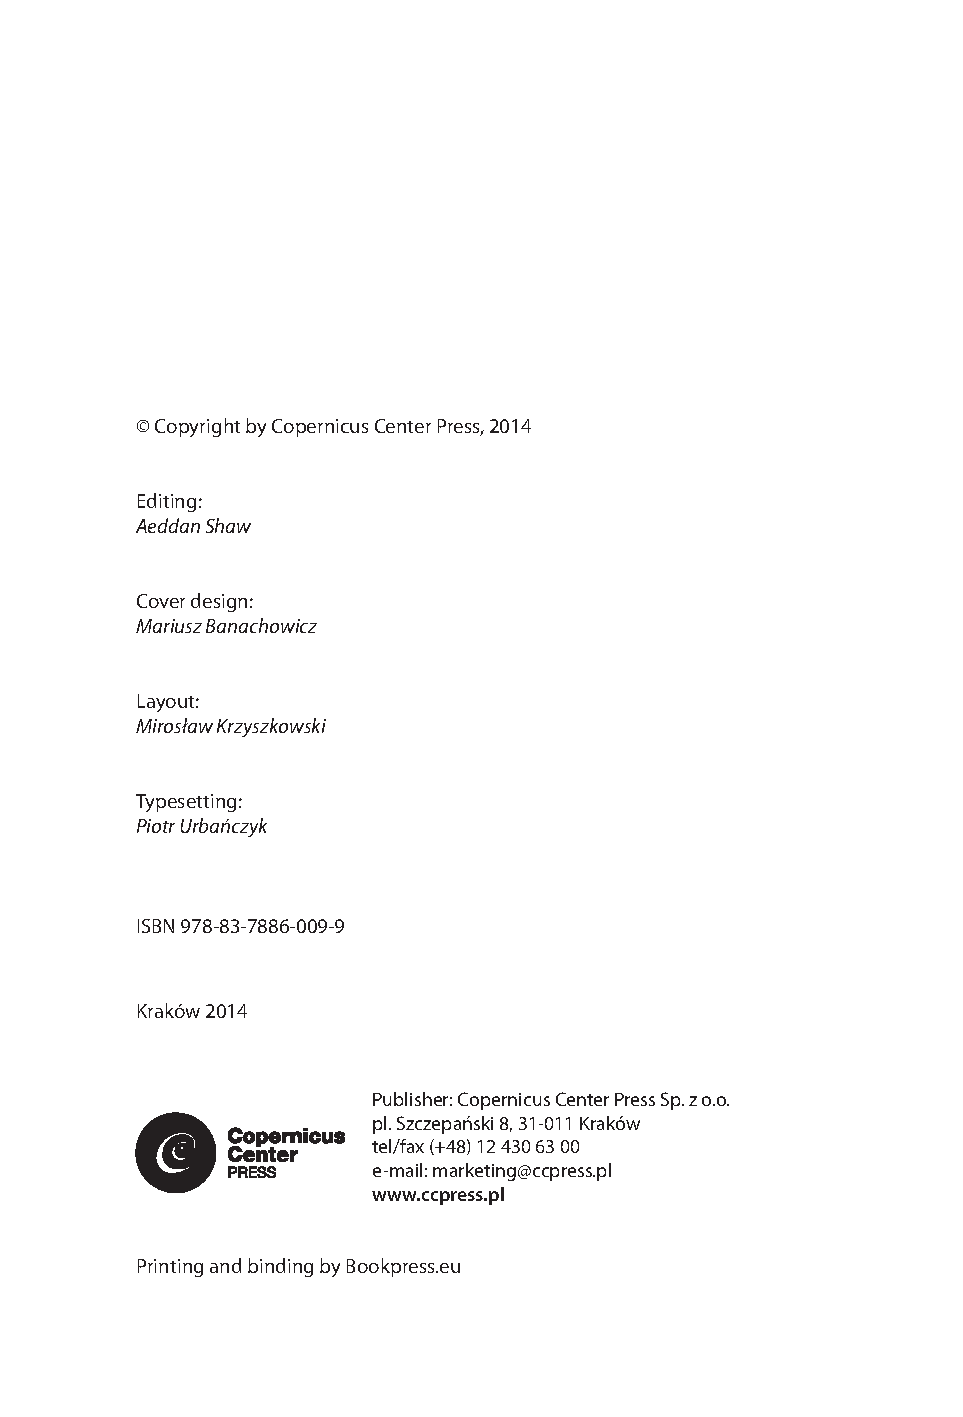
\includepdf[pages=1]{images/CT4.pdf}


\thispagestyle{empty}
\vspace*{1.2in}%
\begin{flushright}
\rectitle{Zagadnienia Filozoficzne\\w Nauce}\par
\vspace*{.5in}%
\chaptitleeng{Philosophical Problems\\in Science}\par
\end{flushright}
\vfill
\clearpage

\thispagestyle{empty}

\vfill

\noindent\begin{czw}© Copernicus Center Press, \rok\end{czw}

\vfill

\begin{adres}
	\begin{pagname}\noindent\begin{czwad}Editorial Board\end{czwad}\\
		Editor-in-Chief: dr hab. Paweł Jan Polak\\
		Deputy Editor-in-Chief: dr hab. Janusz Mączka\\
		Honorary Editor: prof. dr hab. Michał Heller\\
		Guest Editor: dr Tomasz Kwarciński\\
		Editorial Secretary: Piotr Urbańczyk
		
	\end{pagname}
\end{adres}


\vfill

\noindent\begin{czw}Cover design: Mariusz Banachowicz\end{czw}

\vskip.5em

\noindent\begin{czw}Adjustment and correction: Artur Figarski\end{czw}

\vskip.5em

\noindent\begin{czw}Technical editor: Artur Figarski\end{czw}

\vskip.5em

\noindent\begin{czw}Typographic design: Piotr Urbańczyk\end{czw}

\vskip.5em

\noindent\begin{czw}Typeset in \end{czw}\LaTeX

%\noindent\begin{czw}Skład: Artur Figarski\end{czw}


\vfill

\begin{adres}
	\begin{pagname}\noindent ISSN 0867-8286 (print format)\\
		e-ISSN 2451-0602 (electronic format)
	\end{pagname}
\end{adres}

\vfill

\begin{adres}
		\noindent\begin{czwad}Editorial Office\end{czwad}
	
		\noindent\begin{pagname}Zagadnienia Filozoficzne w Nauce
		
		\noindent Wydział Filozoficzny UPJPII
		
		\noindent ul. Kanonicza 9, 31-002 Kraków
		
		\noindent POLAND
		
		\vskip.3em
		
		\noindent e-mail: zagadnienia@upjp2.edu.pl
		
		\noindent www.zfn.edu.pl\end{pagname}
\end{adres}

\vfill

\begin{wrapfigure}{L}{.3\textwidth}
	\noindent\includegraphics[width=.29\textwidth]{images/ccp.pdf}
%\noindent\includegraphics[width=.27\textwidth]{images/ccp.pdf}
\end{wrapfigure}
\vskip.4em
%\noindent\parbox[t]{6cm}{
\begin{adres}
	\noindent\begin{pagname}Publisher: Copernicus Center Press Sp. z o.o.
		
		\noindent pl. Szczepański 8, 31-011 Kraków POLAND
		
		\noindent tel. (+48) 12 448 14 12
		
		\noindent e-mail: marketing@ccpress.pl
		
		\noindent www.ccpress.pl\\ \end{pagname}
	
	
\end{adres}
%}




\clearpage

%	\thispagestyle{empty}
	\begin{flushright}%
	{\bigtitle{Zagadinienia\\Filozoficzne\\w Nauce\par}}%
	\vspace{0.2in}%
	{\chaptitleeng{Philosophical Problems in Science\par}}%
	\vspace{0.2in}%
	\hrule%
	{\LARGE\textbf{{\numerrzymski -- \rok}}}%
	\hrule%
	\end{flushright}%
%		\@mkboth{\czwit\contentsname}{\czwit\contentsname}%
	\vspace{0.5in}%
%
%\clearpage

%Spis tresci -------------------------------------------------

{\thispagestyle{plain} \tableofcontents \clearpage}
%--------------------------------------------------------------------------------------------
\newpage
\thispagestyle{plain}
\cleardoublepage
\thispagestyle{plain}

%--------------------------------------






%\ramkaart{Imię Nazwisko}
{Tytuł rozdziału.\\\chapsubtit{Podtytuł rozdziału}}
{Tytuł rozdziału. Podtytuł rozdziału}
{Tytuł rozdziału. Podtytuł rozdziału}

\lettrine[loversize=0.13,lines=2,lraise=0.00,nindent=0em,findent=0.2pt]%
{W}{}ielu filozofów i językoznawców twierdziło, że gdy identyfikujemy przedmioty, zarówno w języku, jak i w postrzeganiu, kierujemy się względami praktycznymi, potrzebami, wolą -- krótko mówiąc, swego rodzaju interesem, czy to gatunkowym (a więc ogólnoludzkim), czy to swoistym dla danej społeczności, cywilizacji czy jednostki. Wydaje się to kłócić z przeświadczeniem, że te przedmioty muszą istnieć, chyba że traktujemy to przeświadczenie jako jedną z wielu równouprawnionych wizji świata. Ta sama zasada wielości równosilnych perspektyw stosuje się a fortiori do języka metafizyki.

Tak więc powracamy tam, gdzie nasz horror bierze swój początek. Jakże mam trwać przy danym języku (czy jakimś szczególnym punkcie widzenia, z którego patrzę na świat, albo regule interpretacji całości doświadczenia), nie przyznając mu uprzywilejowanej poznawczej mocy? A jeśli pretenduję do dysponowania wyższym czy może nawet absolutnym językiem, to albo nadawałby się on tylko do mówienia o innych językach, nie zaś o rzeczywistości, do której się odnoszą, albo byłby standardowym językiem, a inne byłyby jego niekompletnymi dialektami. W tym drugim przypadku byłby to rzeczywiście boski język, absolutny i zawierający wszelkie wyobrażalne punkty widzenia. Lecz język taki jest niemożliwy; nawet Bóg, przemawiając ustami proroka, musiał się przełożyć na język ludzki; przekład jest niechybnie zniekształcony, a nam brak dostępu do oryginału. W przypadku pierwszym język mój (język pierwszego stopnia, język rzeczy) nie może wprawdzie rościć sobie pretensji do jakiejkolwiek pozycji uprzywilejowanej, lecz w tym języku nie sposób byłoby nieobecność owej pozycji wyrazić: by to uczynić, musiałbym swój język porzucić i przejść do super(czy meta-) języka -- ale w takim języku moje stanowisko, jako że szczególne, nie dałoby się wyrazić.

\myquote{
Gdy więc wielkodusznie powiadam: „wszystkie stanowiska metafizyczne są równie dobre”, sam żadnego stanowiska nie zajmuję, po prostu wyrażam zasadę tolerancji, która, jakkolwiek chwalebna, ma charakter formalny i nigdy nie wyda, czy choćby zainspiruje, żadnej metafizycznej idei. Lecz próbując zachować tę zasadę i obstawać zarazem przy swym szczególnym punkcie widzenia, popadam w niekonsekwencję, jako że twierdzę wtedy, iż „stanowisko moje jest tak samo dobre jak każde inne, mimo że jest nie do pogodzenia z żadnym innym”.

A jeśli tak mówię, nie mogę w zrozumiały sposób wyjaśnić, w jakim sensie to stanowisko jest moje, w przeciwieństwie do innych. Niestety, tolerancyjna wspaniałomyślność nie pozwala uciec od paradoksu samoodniesienia.
}

\noindent Leon Chwistek, logik i malarz, w wydanej w 1921 roku książce Wielość rzeczywistości sugerował istnienie czterech rodzajów wzajemnie niezależnych (a zatem przypuszczalnie nieinterferujących z sobą wzajem) rzeczywistości: rzeczy, takie jak je postrzega zdrowy rozsądek; rzeczy nauk fizycznych; wrażeń; i wyobraźni. Znajdują one swój artystyczny wyraz w malarstwie – odpowiednio: prymitywistycznym, naturalistycznym, impresjonistycznym, futurystycznym\footnote{To jest przypis dolny. Jeśli niezależne od siebie pokłady rzeczywistości wymagają dla swego opisu niezależnych języków, sugeruje to, że języki te są całkowicie nieprzekładalne; skoro tak, to w istocie można sądzić, że różne wizje świata współistnieć mogą w doskonałej wzajemnej obojętności}. Lecz wielość ta, dowodził, pozwala na dowolną liczbę równoprawnych poglądów na świat, z których żadnego nie można dowieść, lecz każdy jest do przyjęcia pod warunkiem, że nie próbuje zmonopolizować prawdy. Dopuszczalne stają się różne odpowiedzi na tradycyjne pytania, jak te o wolność woli, relację między ciałem a duchem, obiektywność wartości, jeśli zakres odniesienia ogranicza się do jednej lub niektórych spośród owych czterech rzeczywistości.

\noindent Leon Chwistek, logik i malarz, w wydanej w 1921 roku książce Wielość rzeczywistości sugerował istnienie czterech rodzajów wzajemnie niezależnych (a zatem przypuszczalnie
nieinterferujących z sobą wzajem) rzeczywistości: rzeczy, takie jak je postrzega zdrowy rozsądek

\section{Podtytuł 1 stopnia}

\noindent Teoria wielu -- jakkolwiek wyodrębnianych -- rzeczywistości, jeśli nawet w tym przypadku stworzona dla metafizycznej interpretacji malarstwa, proponuje przekonujący i kuszący obraz świata. Jednakże jako propozycja epistemologiczna nie jest w stanie -- czy to w wersji Chwistka, czy Williama Jamesa -- poradzić sobie z wciąż tą samą trudnością: jak dowieść wyższości pewnej teorii bytu w tym samym języku, w którym została wypowiedziana? Mieliżbyśmy utrzymywać, że twierdzenie „wszystko jest konieczne” jest równie prawomocne co twierdzenie „poza związkami logicznymi nic nie jest konieczne” i że doktryna, według której słowo „ja” nie ma odniesienia, jest nie mniej prawdziwa niż ta, wedle której cokolwiek ma odniesienie, jest względne w stosunku do „ja”?

\subsection{Podtytuł 2 stopnia}

\noindent Jeśli niezależne od siebie pokłady rzeczywistości wymagają dla swego opisu niezależnych języków, sugeruje to, że języki te są całkowicie nieprzekładalne; skoro tak, to w istocie można sądzić, że różne wizje świata współistnieć mogą w doskonałej wzajemnej obojętności: nie mogą być ze sobą konfrontowane ani między sobą sprzeczne. Ale twierdzenie, że nie mogą być konfrontowane, jest wyrażone w języku innym, wyższego stopnia, nie nadającym się do celów metafizycznych. I tu powraca ten sam kłopot: albo ograniczamy się do tego wyższego języka i wtedy werdykty nasze nie mają znaczenia dla rzeczywistych problemów, z których filozofia żyje, albo przyjmujemy pewną metafizyczną perspektywę i głosimy, że perspektywy tej, jako zamkniętej, nie da się zharmonizować z żadną inną ani też innej przeciwstawić -- i wtedy też, w wyniku tej samointerpretacji, perspektywa nasza jest bez znaczenia dla rzeczywistych problemów, z których filozofia żyje.

\sectionno{Podtytuł 1 stopnia}

\noindent Teoria wielu -- jakkolwiek wyodrębnianych -- rzeczywistości, jeśli nawet w tym przypadku stworzona dla metafizycznej interpretacji malarstwa, proponuje przekonujący i kuszący obraz świata. Jednakże jako propozycja epistemologiczna nie jest w stanie -- czy to w wersji Chwistka, czy Williama Jamesa -- poradzić sobie z wciąż tą samą trudnością: jak dowieść wyższości pewnej teorii bytu w tym samym języku, w którym została wypowiedziana? Mieliżbyśmy utrzymywać, że twierdzenie „wszystko jest konieczne” jest równie prawomocne co twierdzenie „poza związkami logicznymi nic nie jest konieczne” i że doktryna, według której słowo „ja” nie ma odniesienia, jest nie mniej prawdziwa niż ta, wedle której cokolwiek ma odniesienie, jest względne w stosunku do „ja”?

\subsection{Podtytuł 2 stopnia}

\noindent Jeśli niezależne od siebie pokłady rzeczywistości wymagają dla swego opisu niezależnych języków, sugeruje to, że języki te są całkowicie nieprzekładalne; skoro tak, to w istocie można sądzić, że różne wizje świata współistnieć mogą w doskonałej wzajemnej obojętności: nie mogą być ze sobą konfrontowane ani między sobą sprzeczne. Ale twierdzenie, że nie mogą być konfrontowane, jest wyrażone w języku innym, wyższego stopnia, nie nadającym się do celów metafizycznych. I tu powraca ten sam kłopot: albo ograniczamy się do tego wyższego języka i wtedy werdykty nasze nie mają znaczenia dla rzeczywistych problemów, z których filozofia żyje, albo przyjmujemy pewną metafizyczną perspektywę i głosimy, że perspektywy tej, jako zamkniętej, nie da się zharmonizować z żadną inną ani też innej przeciwstawić -- i wtedy też, w wyniku tej samointerpretacji, perspektywa nasza jest bez znaczenia dla rzeczywistych problemów, z których filozofia żyje.

\section{Podtytuł 1 stopnia}

\noindent Teoria wielu -- jakkolwiek wyodrębnianych -- rzeczywistości, jeśli nawet w tym przypadku stworzona dla metafizycznej interpretacji malarstwa, proponuje przekonujący i kuszący obraz świata. Jednakże jako propozycja epistemologiczna nie jest w stanie -- czy to w wersji Chwistka, czy Williama Jamesa -- poradzić sobie z wciąż tą samą trudnością: jak dowieść wyższości pewnej teorii bytu w tym samym języku, w którym została wypowiedziana? Mieliżbyśmy utrzymywać, że twierdzenie „wszystko jest konieczne” jest równie prawomocne co twierdzenie „poza związkami logicznymi nic nie jest konieczne” i że doktryna, według której słowo „ja” nie ma odniesienia, jest nie mniej prawdziwa niż ta, wedle której cokolwiek ma odniesienie, jest względne w stosunku do „ja”?

\subsection{Podtytuł 2 stopnia}

\noindent Jeśli niezależne od siebie pokłady rzeczywistości wymagają dla swego opisu niezależnych języków, sugeruje to, że języki te są całkowicie nieprzekładalne; skoro tak, to w istocie można sądzić, że różne wizje świata współistnieć mogą w doskonałej wzajemnej obojętności: nie mogą być ze sobą konfrontowane ani między sobą sprzeczne. Ale twierdzenie, że nie mogą być konfrontowane, jest wyrażone w języku innym, wyższego stopnia, nie nadającym się do celów metafizycznych. I tu powraca ten sam kłopot: albo ograniczamy się do tego wyższego języka i wtedy werdykty nasze nie mają znaczenia dla rzeczywistych problemów, z których filozofia żyje, albo przyjmujemy pewną metafizyczną perspektywę i głosimy, że perspektywy tej, jako zamkniętej, nie da się zharmonizować z żadną inną ani też innej przeciwstawić -- i wtedy też, w wyniku tej samointerpretacji, perspektywa nasza jest bez znaczenia dla rzeczywistych problemów, z których filozofia żyje.

\begin{thebibliography}{00}{Imię Nazwisko}
{Tytuł rozdziału. Podtytuł rozdziału}

\makeatletter
    \clubpenalty10000
    \@clubpenalty \clubpenalty
    \widowpenalty10000
\makeatother


\bibitem{Abc}
A.~Abc, \textit{Abc}...

\bibitem{Xyz}
A.~Abc, \textit{Abc}...

\end{thebibliography}





\sekcja{Od Redakcji}{Editorial}

\begin{editorial}{Tomasz Kwarciński}
	{Filozofia ekonomii -- szkoła pluralizmu i~pokory}
	{Filozofia ekonomii -- szkoła pluralizmu i~pokory}
	{Filozofia ekonomii -- szkoła pluralizmu i~pokory}
	%	{Copernicus Center for Interdisciplinary Studies}
	{Philosophy of economics -- a~school of pluralism and humility}
	%	{Abstrakt lorem ipsum}
	%	{słowo, słowo.}




\lettrine[loversize=0.13,lines=2,lraise=-0.05,nindent=0em,findent=0.2pt]%
{P}{}o raz pierwszy w~historii \textit{Zagadnień Filozoficznych w~Nauce} prezentujemy Czytelnikom numer w~całości poświęcony
filozoficznej refleksji nad ekonomią.  Tematyka poruszana w~poszczególnych artykułach daje wyraz potrzebie pluralizmu
dociekań ekonomicznych, który domaga się wyjścia poza ramy metodologii ekonomii głównego nurtu, uwzględnienia założeń
wartościujących w~modelach ekonomicznych, wzięcia pod uwagę dorobku ekonomicznej heterodoksji oraz poddawania
przeświadczeń ekonomistów krytycznej refleksji. Wszystko to w~czasie, w~którym z~jednej strony część profesji
ekonomicznej oraz studentów ekonomii po doświadczeniu negatywnych skutków kryzysu finansowego 2008 r. doszła do
wniosku, że nadziei na uniknięcie podobnych wydarzeń w~przyszłości trzeba szukać w~większym otwarciu badań i~standardów
edukacji ekonomicznej, uwzględniającym pluralizm poglądów ekonomicznych. Z~drugiej zaś strony, w~okresie, w~którym
wciąż, zarówno na świecie, jak i~w~Polsce na uczelniach ograniczana jest liczba godzin lub likwidowane są kursy
metodologii ekonomii bądź historii myśli ekonomicznej. Tym bardziej cieszy więc fakt, że wśród młodych
ekonomistów i~filozofów znajdują się ludzie, którzy poświęcają swój czas i~energię na metarefleksję nad ekonomią. 

W niniejszym numerze ZFN znajdziemy zarówno teksty osób, które są na wczesnym etapie rozwoju naukowego, jak i~recenzje
prac uznanych naukowców. Znajdziemy tu zarówno teksty dotyczące zagadnień metodologicznych w~ekonomii,
jak i~interpretacji historycznych klasyków ekonomii, a~także prace poświęcone problematyce normatywnych założeń teorii
ekonomicznych. Do pierwszej grupy należy tekst Krzysztofa Turowskiego ,,Mikropodstawy prawdziwe i~fałszywe'', w~którym
przedstawiona została krytyka dwóch podejść w~modelowaniu makroekonomicznym, podejścia skoncentrowanego na agregatach
ekonomicznych typu: PKB, wskaźniki inflacji, agregaty pieniężne, które charakteryzuje się oderwaniem analizy
ekonomicznej od poziomu działań indywidualnych ludzi oraz podejścia poszukującego mikropodstaw zjawisk
makroekonomicznych. Autor nie tylko przedstawia krytykę obu stanowisk lecz także formułuje postulaty, które spełniać
powinny teorie z~adekwatnymi mikropodstawami. Na koniec, wyraża przekonanie, że w~poszukiwaniu mikropodstaw modeli
ekonomicznych może pomóc uwzględnianie postulatów szkół heterodoksyjnych (np. post-keynesismu, szkoły austriackiej),
a~także krytyczna refleksja metodologiczna i~historyczna.

Kolejną fundamentalną kwestię metodologiczną porusza tekst Bartosza Kurkowskiego ,,Czy konstruktywiści społeczni mówią
nam o~czymś realnym w~ekonomii?''. Tytułowe pytanie wskazuje na spór toczony między zwolennikami dwóch stanowisk
epistemologicznych w~ekonomii, czyli konstruktywizmu i~realizmu, które operują odmiennymi koncepcjami
prawdy i~rzeczywistości. Autor stawia sobie za cel sprawdzenie, ,,czy można mówić o~realnych
zjawiskach i~mechanizmach w~gospodarce, nawet jeśli nie istnieją one poza ludzkimi umysłami''.
Opowiadając się ostatecznie za stanowiskiem pełnej
intersubiektywności stwierdza, że w~odniesieniu do zjawisk ekonomicznych staje się ona ich obiektywnością. To z~kolei
prowadzi do uznania, że można mówić o~realnych zjawiskach i~mechanizmach gospodarczych, nawet jeśli nie istnieją one
poza ludzkimi umysłami. 

Krzysztof M. Turek osadza dyskusję na temat kluczowego założenia teorii ekonomicznych, czyli założenia o~racjonalności,
w~kontekście historycznym. W~artykule zatytułowanym ,,W poszukiwaniu racjonalności ekonomicznej w~dziełach Adama Smitha''
stara się odpowiedzieć na pytanie, czy w~pracach ,,ojca ekonomii'' znajdują się już zalążki koncepcji rozwijanej
współcześnie w~ramach teorii racjonalnego wyboru, która może służyć za teoretyczną podbudowę tzw. kultury chciwości,
zgodnej z~maksymą \textit{greed is good}. W~tym celu sięga do głównych dzieł Smitha, czyli \textit{Teorii uczuć
moralnych} oraz \textit{Badań nad naturą i~przyczynami bogactwa narodów}. Autor dochodzi do wniosku, że w~pracach
Smitha możemy się raczej doszukiwać inspiracji do formułowania sprzeciwu wobec kultury chciwości. 

Poglądy Adama Smitha stały się również przedmiotem analiz Filipa Lubińskiego, który w~tekście ,,Rola
państwa i~prawa w~systemie Adama Smitha'' stawia sobie za cel rekonstrukcję poglądów na temat systemu społecznego,
za którym opowiadał się
szkocki filozof. Poza najbardziej znanymi dziełami Smitha dotyczącymi etyki i~ekonomii Autor sięga do rzadziej
analizowanej pracy, którą jest \textit{Lectures on Jurisprudence}. Dochodzi przy tym do wniosku, że ,,ojciec ekonomii''
nie tylko nie był zwolennikiem państwa minimum, określanego mianem ,,stróża nocnego'', lecz na bazie jego prac daje się
zrekonstruować teorię uprawnień efektywnych, zgodnie z~którą, władza powinna gwarantować obywatelom szeroki wachlarz
uprawnień politycznych i~ekonomicznych oraz dbać o~materialne podstawy umożliwiające im realizację tych uprawnień.
Teoria uprawnień efektywnych Smitha opiera się na przyjmowanych przez niego założeniach etycznych, a~także służy
osiąganiu w~gospodarce najwyższego możliwego dobrobytu. 

Kolejne dwa teksty rozwijają kwestie założeń wartościujących (w tym etycznych) w~ekonomii oraz interpretacji i~pomiaru
dobrobytu. W~artykule ,,Droga ekonomii wolnej od wartościowania do epistemologicznej pychy. Użycie i~nadużycie
matematyki przez ekonomistów'' Aleksander Ostapiuk dowodzi, że pomimo krytyki dominujący paradygmat ekonomii
neoklasycznej nie ulega zmianie, gdyż opiera się na aksjomatycznych założeniach teorii wolnej od wartościowania. Autor
dokonuje analizy tych założeń na przykładzie podejścia ekonomicznego Gary’ego Beckera interpretując je przez pryzmat
koncepcji programów badawczych Imre Lakatosa. Na bazie tych rozważań Autor formułuje również postulat otwarcia się
ekonomii na koncepcje normatywne oraz pluralizm metodologiczny.

Bez wątpienia jedną z~najistotniejszych normatywnych koncepcji w~ekonomii jest koncepcja dobrobytu. W~tekście ,,Problem
istoty i~pomiaru dobrobytu'' Wojciech Rybka dokonuje przeglądu najważniejszych filozoficznych i~ekonomicznych koncepcji
dobrobytu, wskazując jednocześnie trudności towarzyszące każdej z~nich. Autor wyróżnia dobrobyt ogólny, dobrobyt
ekonomiczny (materialny) oraz dobrobyt subiektywny. Na tle pozostałych artykułów pracę Rybki wyróżnia fakt, że nie 
poprzestaje on na teoretycznych rozważaniach, i~w~odniesieniu do dobrobytu przechodzi od kwestii pojęciowych do sposobów
operacjonalizacji tego pojęcia poprzez odpowiednie wskaźniki (HDI dla dobrobytu ogólnego, PKB dla dobrobytu
ekonomicznego oraz SWB dla dobrobytu subiektywnego). Następnie, na przykładzie wybranych krajów sprawdza jak bardzo
wyróżnione wskaźniki są ze sobą skorelowane oraz bada ich dynamikę w~czasie. 

Tym co łączy wszystkie prezentowane teksty jest nie tylko przekonanie o~ważności pluralizmu ekonomicznego, niestronienie
od kontekstu historycznego lecz także zwracanie uwagi na konieczność ostrożnego formułowania wniosków na podstawie
teorii i~modeli ekonomicznych, swoistej ekonomicznej pokory. Teksty te łączy również fakt, że zostały one nadesłane w
konkursie na esej metaekonomiczny, który w~2018 roku został zorganizowany przez Polską Sieć Filozofii Ekonomii oraz
Polski Instytut Ekonomiczny, przy wsparciu wydawnictwa Copernicus Center Press. 

Dopełnienie prezentowanych w~niniejszym numerze \textit{Zagadnień} artykułów poświęconych filozofii ekonomii stanowią
recenzje książek. Dwie z~nich dotyczą wprost pozycji z~zakresu filozofii ekonomii,
trzecia jest poświęcona popularnonaukowej pracy z~dziedziny etologii,
podejmującej jednak zagadnienia inspirujące tak dla ekonomistów, jak i~filozofów.
Recenzja Marcina Gorazdy, ,,Believable world of economic models'' prezentuje
monografię Łukasza Hardta zatytułowaną \textit{Economics Without Laws. Towards a~New Philosophy of Economics}. Nie
stroniąc od uwag krytycznych wymierzonych w~główną tezę książki, zgodnie z~którą w~ekonomii nie ma praw naukowych,
rozumianych jako aczasowe, uniwersalne regularności, Gorazda zwraca uwagę, że praca stanowi wartościową lekturę zarówno
ze względu na jej bogatą treść, jak i~inspirujące wnioski. Dowodem tego są uwagi polemiczne sformułowane przez Autora
recenzji. 

Drugą recenzowaną publikacją jest praca zbiorowa \textit{Metaekonomia II. Zagadnienia z~filozofii makroekonomii}, której
redaktorom, Tomaszowi Kwarcińskiemu oraz Agnieszce Wincewicz-Price udało się zaprosić grono uznanych ekonomistów i
filozofów z~kraju i~zagranicy (wśród nich Daniel Hausman, Peter Galbács, Jerzy Osiatyński, Marcin Gorazda, Emilia Tomczyk)
do podjęcia
kwestii metodologicznych oraz etycznych związanych z~makroekonomią. Joanna Dzionek-Kozłowska, w~swojej recenzji zwraca
uwagę na
wielość stanowisk, odnoszących się do poruszanych w~pracy zagadnień i~debat filozoficznych,
metodologicznych i~historycznych. Podkreśla jednocześnie, że daje to czytelnikowi
możliwość nie tylko zapoznania się z~bogactwem poglądów z~obszaru filozofii ekonomii, ale i~szansę wyrobienia sobie własnego zdania.

Ostatnią z~recenzowanych prac jest książka Fransa de Waala \textit{Wiek
empatii. Jak natura uczy nas życzliwości}, w~której z~ewolucyjnej
perspektywy analizuje on różne poziomy empatii oraz rolę, jaką ona
odgrywa w~rozmaitych społecznościach zwierzęcych, w~szczególności w~społecznościach
ludzkich. W~recenzji tej pracy Milena Cygan zwraca
uwagę, że jedną z~najważniejszych tez amerykańskiego naukowca jest
przekonanie, iż człowiek z~natury nie jest zły ani antyspołeczny, a~wciąż
występujące w~niektórych kręgach naukowych pozostałości po
darwinizmie społecznym nie wytrzymują konfrontacji z~badaniami
etologicznymi. Autorka kończy recenzję uwagą, że prezentowana
przez nią książka stanowi przykład tego jak nauka może pomagać w~rozwijaniu
refleksji na temat klasycznych problemów filozoficznych, do
których bez wątpienia należy spór o~naturę ludzką. Dodajmy jedynie, iż
spór ten ma swoje miejsce również w~filozofii ekonomii.

\end{editorial}



\sekcja{Artykuły}{Articles}

\begin{artplenv}{Krzysztof Turowski}
	{Mikropodstawy prawdziwe i~fałszywe}
	{Mikropodstawy prawdziwe i~fałszywe}
	{Mikropodstawy prawdziwe i~fałszywe}
	{Uniwersytet Gdański}
	{Microfoundations: true and false}
	{This article presents an overview and critique of the two leading macroeconomic approaches from the last 70 years:
		reasoning using high-level aggregates detached from individuals and their choices, and modeling using so-called
		microfoundations. We judge the validity of both methods, showing their inherent limits and deficiencies as explanatory
		and predictive tools of economics. We also underline several vital improvements, which are required if the models are
		supposed to guide policy decisions -- even if this means a~more modest and less conceited approach.}
	{methodology of economics, history of economic thought, macroeconomics, microfoundations, DSGE.}



\section*{Wprowadzenie}
\lettrine[loversize=0.13,lines=2,lraise=-0.05,nindent=0em,findent=0.2pt]%
{J}{}akkolwiek filozofowie mogą się spierać o~dokładną definicję ekonomii, jej metod i~jej przedmiotu, tak w~codziennej
praktyce i~potocznym postrzeganiu jest to nauka dość dobrze określona i~wyodrębniona spośród nauk społecznych. Widać to
chociażby w~jej strukturze instytucjonalnej: odrębnych wydziałach i~katedrach, własnych specjalistycznych czasopismach
lub konferencjach oraz nagrodach, z~Nagrodą Banku Szwecji im. Alfreda Nobla na czele. W~dużym uproszczeniu można
powiedzieć, że ekonomia zajmuje się wszystkimi zagadnieniami związanymi z~gospodarką oraz gospodarowaniem.

Istnieje szeroka zgoda wśród ekonomistów, odzwierciedlona m.in. w~układzie większości współczesnych podręczników, co do
fundamentalnego podziału dziedziny na mikroekonomię i~makroekonomię. Mikroekonomia zajmuje się
zjawiskami z~indywidualnego punktu widzenia, m.in. rozpatruje determinanty oraz skutki decyzji konsumentów i~producentów, wyjaśnia
zależności cen, podaży i~popytu czy też bada firmę w~jej danym otoczeniu gospodarczym. Makroekonomia traktuje natomiast
o~fenomenach dotyczących całej gospodarki np. o~dochodzie narodowym, wzroście gospodarczym, kryzysach, inflacji czy
bezrobociu, jak również o~handlu międzynarodowym
\parencite{samuelson_ekonomia_2003}.
%\label{ref:RNDAXNmHXMliV}(Samuelson, Nordhaus, 2003).

Związek między obydwoma sferami wydaje się intuicyjnie oczywisty: bez indywidualnych wyborów jednostek nie istniałaby
gospodarka jako całość. To, co istnieje na poziomie całej gospodarki z~konieczności jest nabudowane na decyzjach
jednostek, zatem teoria mikroekonomiczna i~makroekonomiczna powinny pozostawać w~ścisłym systematycznym związku. Co
więcej, wielu ekonomistów przynajmniej deklaratywnie przyjmuje metodologiczny indywidualizm, czyli tezę o~potrzebie
wyjaśniania zjawisk ekonomicznych przez odwołanie do subiektywnych ocen i~wartościowań jednostek.  W~tym ujęciu
makroekonomia powinna być raczej pewnym rozwinięciem i~uzupełnieniem mikroekonomii o~zależności wynikające z~agregacji
działań w~całej gospodarce oraz interakcji między różnymi grupami lub sektorami.

Z drugiej strony, istnieje w~ekonomii długa tradycja wyjaśniania zjawisk makroekonomicznych na poziomie abstrakcyjnych
agregatów, nieprzekładalnych wprost na poszczególne procesy na poziomie jednostkowym. Przykładami tego mogą być
rozważania merkantylistów dot. czynników gospodarczych determinujących bogactwo narodów, fizjokratyczne \textit{Tableau
economique} pokazujące przepływy dochodów między poszczególnymi grupami w~gospodarce, a~z~bardziej współcześnych np.
model AS-AD, wiążący poziom cen i~produkcji w~gospodarce ze zagregowanym popytem i~podażą.

Celem niniejszego artykułu jest przedstawienie oraz krytyka dwóch popularnych w~ostatnich 70 lat podejść
makroekonomicznych: nieco wcześniejszego, ujęcia zjawisk według bardzo ogólnych kategorii, oderwanych od poziomu
jednostek i~ich działań, oraz dominującego od lat osiemdziesiątych ubiegłego wieku tzw. modelowania z~mikropodstawami.
Przedstawiona zostanie krytyka obu metod w~kontekście ich zasadności jako narzędzi w~teorii ekonomii oraz wskazane
zostaną ograniczenia ich stosowalności do oceny i~doboru polityki gospodarczej państwa. Dodatkowo, zostaną
przedstawione pewne ogólne postulaty, których uwzględnienie mogłoby znacząco wspomóc lub uzupełnić obecnie stosowane
metody -- a~które to postulaty stanowiły fundament wielu wartościowych wglądów dokonanych przez
ekonomistów w~przeszłości, nakierowanych na zachodzące realnie procesy gospodarcze

\section{Makroekonomia bez mikropodstaw}
W pierwszych dekadach po II wojnie światowej makroekonomia została zdominowana przez podejście skoncentrowane na
szukaniu relacji między zmiennymi obejmującymi całość gospodarki, takimi jak zagregowany popyt i~podaż, całkowita
produkcja, bezrobocie, poziom cen czy inflacja. Wśród sztandarowych przykładów tego typu podejścia należy wymienić tzw.
krzyż keynesowski (wiążący zagregowany popyt i~realną produkcję), model IS-LM (wyrażający zależność stopy
procentowej i~realnej produkcji), a~także krzywą Philipsa (opisującą postulowaną zależność między inflacją a~bezrobociem).
Modele gospodarcze składały się typowo z~kilku zmiennych, a~zadaniem ekonomistów była analiza interakcji tych zmiennych
%\label{ref:RNDN3QnGZQIJq}(Lachmann, 1973)
\parencite{lachmann_macro-economic_1973}\footnote{Typowym przykładem takiego podejścia jest \textit{Money, Interest,
and Prices}
\parencite{patinkin_money_1956}.
%\label{ref:RNDe8wVA5c7uE}(Patinkin, 1956).
}.

Przyczyn takiego stanu rzeczy można wskazać kilka: przede wszystkim istotny był proces recepcji \textit{Ogólnej teorii
zatrudnienia, produkcji i} \textit{pieniądza} Johna Maynarda Keynesa
\parencite*{keynes_general_1936},
%\label{ref:RND5MranCHmpU}(1936),
która szybko
zdobyła popularność wśród młodych, zdolnych ekonomistów m.in. Johna Hicksa, Franco Modiglianiego czy Paula Samuelsona
\parencite{moggridge_diffusion_1995}.
%\label{ref:RNDnBqm7Ivc9s}(Moggridge, 1995).
To właśnie oni dokonali formalizacji i~matematyzacji ujęć
keynesowskich w~ramach wyżej wymienionych modeli\footnote{Nawet mimo wprost uznania modelu IS-LM przez Keynesa za właściwą
interpretację \textit{Ogólnej teorii}
\parencite{king_history_2003},
%\label{ref:RND0kaWblMGjk}(King, 2003),
wielu ekonomistów wskazuje, że u~Keynesa
istnieją również ważne elementy mikroekonomiczne np. dotyczące oczekiwań i~niepewności, które są sprzeczne z~tzw.
syntezą neoklasyczną
\parencite{leijonhufvud_keynes_1969}.
%\label{ref:RNDs0gQMcriAO}(Leijonhufvud, 1969).
Joan Robinson wręcz nazywała powojenną
podręcznikową interpretację Keynesa ,,zwulgaryzowaną'' i~,,bękarcią''
\parencite{robinson_what_1974}.
%\label{ref:RNDsTNNR3eOoV}(Robinson, 1974).
}. Co
ważniejsze, olbrzymi sukces podręcznika Samuelsona upowszechnił te ujęcia, tworząc podstawy nauczania nowej ortodoksji,
w~której zagadnienia makroekonomiczne rozważano w~zasadniczym oddzieleniu od teorii mikroekonomii, przede wszystkim
traktującej o~alokacji dóbr przez racjonalnych maksymalizatorów w~danym otoczeniu i~systemie cenowym
%\label{ref:RNDA51vqkdiYx}(Colander, Landreth, 1996)
\parencite{colander_coming_1996}\footnote{Weintraub
\parencite*{weintraub_microfoundations:_1979}
%\label{ref:RNDiHw3ZZgTLu}(1979)
wskazuje na to,
że perspektywa mikroekonomiczna wychodzi od badania wyborów jednostek przy danych ograniczeniach, natomiast perspektywa
makroekonomiczna niejawnie zaprzecza, że dezagregacja jest jakkolwiek przydatna w~kontekście predykcji.}.

Źródeł opisywanych zmian zainteresowań ekonomistów można także szukać na zewnątrz. Z~jednej strony, lata międzywojenne
były okresem niestabilności gospodarczej, co naturalnie orientowało zainteresowania ekonomistów na problem kryzysów
gospodarczych oraz ich zapobiegania i~przezwyciężania. Z~drugiej strony, powstanie ZSRS, wdrażającej w~życie
pełnoskalową gospodarkę planową, rozbudziło dyskusje dot. wzrostu gospodarczego oraz właściwej roli polityki
gospodarczej w~tym procesie.

Równolegle można było zaobserwować powstanie systematycznego podejścia do badań empirycznych nad gospodarką.
Symbolicznym początkiem stało się ustanowienie w~roku 1930 Econometric Society oraz założenie w~1932 roku Komisji
Cowlesa (pod hasłem \textit{Science is measurement}), zorientowanej na podejście ilościowo-statystyczne. Zaczęły
powstawać coraz bardziej skomplikowane ilościowe modele gospodarcze autorstwa Jana Tinbergena, Lawrence’a Kleina oraz
wielu innych, starające się zasypać przepaść między ekonometrią a~teorią ekonomii oraz mające umożliwiać zarówno
przewidywanie zmian aktywności gospodarczej, jak i~porównywanie alternatywnych rozwiązań politycznych, a~zatem
zapewniać naukowe uzasadnienie dla państwowego nadzoru nad gospodarką
\parencite{de_vroey_keynesian_2012}.
%\label{ref:RNDQfzjK0pDtC}(De Vroey, Malgrange, 2012).

Nałożyło się na to ogólne fizykalistyczno-inżynierskie podejście do zagadnień ekonomicznych, mające swoje źródło jeszcze
w~XIX w.
\parencite{mirowski_more_1999}.
%\label{ref:RNDcTF11CDYlQ}(Mirowski, 1999).
Przykładowo, Irving Fisher uzasadniając głoszoną przez siebie
ilościową teorię pieniądza wprost pisał, że istnieje pełna analogia między prawem Boyle’a a~równaniem wymiany, w~którym
rolę cząsteczek gazu spełniają działające jednostki
%(Fisher, 1922)
\parencite{fisher_purchasing_1922}\footnote{Na marginesie warto dodać, że promotorem
doktoratu Fishera w~Yale był fizyk, specjalista od termodynamiki, Willard Gibbs.}. To podejście można zresztą
zaobserwować do dziś np. w~twierdzeniu, że modelowanie ekonomiczne nie różni się fundamentalnie od przewidywań
meteorologicznych lub epidemiologicznych, w~których nie analizuje się konkretnych jednostkowych interakcji np. atomów
czy, ale efekty globalne
\parencite{buchanan_forecast:_2013}.
%\label{ref:RNDZuwuTK5nIV}(Buchanan, 2013).

Istnieje jednak poważna różnica: w~przypadku ekonomii przedmiotem na poziomie mikro są ludzie, którzy są znacząco
heterogeniczni, mają różne plany i~cele, nawet w~obiektywnie identycznych okolicznościach, podczas gdy atomy czy nawet
bakterie takiej właściwości zgodnie z~naszą wiedzą nie mają, w~związku z~tym wiadomo, że analogia na pewno nie jest
poprawna w~istotnym aspekcie
\parencite{penrose_biological_1952}.
%\label{ref:RND4t79oENLHg}(Penrose, 1952).
Co więcej, można przywołać w~tym miejscu
modyfikację popperowskiego argumentu przeciw historycyzmowi: ludzie są zdolni do uczenia się, modyfikacji swojego
zachowania, a~więc nie można traktować ich jako stałych i~niezmiennych przedmiotów działania wielkich sił, czy to
dziejowych, czy gospodarczych
\parencite{popper_poverty_1957,hoppe_economic_1995}.
%\label{ref:RNDLB8WeG6ZxD}(Popper, 1957; Hoppe, 1995).

W gruncie rzeczy, stosując takie podejście i~ignorując wiedzę o~poziomie mikroekonomicznym dokonujemy świadomej
rezygnacji z~wiedzy o~różnorodności i~zmienności zachowań jednostek. Zamiast jednak dokonywać abstrakcji
nieprecyzującej  --  a~więc uznać, że skutki tej heterogeniczności są nieznane i~zająć się badaniem tego, co od
nich niezależne  --  to dokonywana jest raczej asercja jawnie fałszywej zasady, mówiącej że struktura zachowań
jednostek nie ma znaczącego wpływu na relacje między agregatami makroekonomicznymi
\parencite{long_realism_2006}.
%\label{ref:RND1jtnbEDYR6}(Long, 2006).

Ujęcie makroekonomiczne oparte jedynie o~wysokopoziomowe agregaty napotyka na inny podstawowy problem
metodologiczny: w~przytoczonym przypadku gazów posiadamy dobre operacyjne ujęcie temperatury czy objętości
gazu, a~więc jego właściwości
makroskopowych. Wręcz to te cechy są pierwotne w~porządku poznania wobec teoretycznego modelu atomowego, stanowiącego
wyjaśnienie na poziomie mikro. Natomiast w~ekonomii mamy do czynienia z~sytuacją odwrotną: bezpośrednio obserwujemy
poszczególne wymiany dóbr i~usług w~gospodarce pieniężnej, konkretne zmiany zatrudnienia, ale już treści pojęć ,,podaż
pieniądza'' czy ,,bezrobocie'' jest znacznie trudniej uchwytna. Dość powiedzieć, że dość szeroko stosowane jest aż pięć
miar agregatowej podaży pieniądza (M\textsubscript{0}{}-M\textsubscript{3} oraz MZM)\footnote{Zob. Federal Reserve Bank
of St. Louis: \url{https://fred.stlouisfed.org/categories/24}} oraz sześć miar bezrobocia\footnote{Zob. Bureau of Labor
Statistic: \url{https://www.bls.gov/news.release/empsit.t15.htm}}, z~których żadna nie może być niearbitralnie
wyróżniona jako ta ,,właściwa''. Joseph Schumpeter
\parencite*{schumpeter_nature_2010}
%\label{ref:RNDBDWQZcLJxs}(2010)
ujmował to dosadnie:

\myquote{
Nie będziemy więcej zainteresowani nimi [pojęciami ,,dochodu narodowego'', ,,bogactwa narodowego'',
,,kapitału społecznego'' -- przyp. aut.]. Gdybyśmy jednak to zrobili,
to dostrzeglibyśmy jak wielkie są ich niejasności i~trudności, i~że są blisko
związane z~rozlicznymi fałszywymi poglądami, nie prowadząc do ani jednego naprawdę ważnego aksjomatu\footnote{``[\mydots] we
will not even deal with them any more; if we would do it, it would become clear the amount of vagueness and problems
attached to it, that they are closely related with a~lot of skewed opinions, without leading to just one really
important axiom'' (jeśli nie zaznaczono inaczej wszystkie tłumaczenia są własne).}.
}

Oskar Morgenstern wskazywał na inną znaczącą różnicę: obserwacje makroekonomiczne są obciążone dokładnie tymi samymi
błędami, co obserwacje w~naukach przyrodniczych, ale również mają szereg własnych problemów, wynikających z~braku
zaplanowanych eksperymentów, unikalności zjawisk, ukrytych zależności czy problematyczności wiarygodności
kwestionariuszy. W~rezultacie, poprawna praktyka badawcza sugerowałaby konieczność zdecydowanie bardziej
ostrożnego i~wymagającego podejścia do zdobywania danych gospodarczych. Jednocześnie, nie sposób nie zauważyć,
że ekonomia, w~odróżnieniu od nauk przyrodniczych nie wypracowała aż tak rygorystycznego podejścia do błędów obserwacji. Niższe
standardy pomiarowe znajdują swoje odzwierciedlenie w~jakości zdobywanych informacji, które mimo tego są przedstawiane
jako pełnowartościowe w~debacie publicznej oraz stanowią materiał do modelowania dla innych ekonomistów, będących tylko
konsumentami pracy pomiarowej
\parencite{morgenstern_accuracy_1963}.
%\label{ref:RNDO4EkQydA8d}(Morgenstern, 1963).

Jak wskazywał Ludwig Lachmann, część miar agregatowych jest konstruowana przy założeniu, że gospodarka znajduje
się w~stanie równowagi ogólnej. Produkt Krajowy Brutto, aby adekwatnie móc agregować nominalną wartość produktów, wymaga,
żeby istniała pełna zgodność planów producentów i~konsumentów w~strukturze kapitałowej. Jeśli pewien proces produkcji
zostanie przerwany na pewnym etapie z~uwagi na brak popytu na dobro końcowe, to należy raczej mówić o~błędnej alokacji
kapitału niż o~czymś, co należy zaliczyć do wartościowej całkowitej produkcji. Co więcej, PKB jest miarodajne tylko
przy założeniu równowagi w~systemie elastycznych cen, dostosowujących się do planów działających jednostek. Jeśli
natomiast w~gospodarce istnieje szeroka kontrola cen (w postaci cen minimalnych/maksymalnych czy płac minimalnych), to
w~zasadzie dokonywana jest agregacja dość arbitralnych liczb, a~więc trudno mówić o~miarodajnym oddaniu poziomu
zasobności społeczeństwa
\parencite{lachmann_macro-economic_1973}.
%\label{ref:RNDL1VjrxjgN6}(Lachmann, 1973).
Dobrą ilustracją tego problemu są dane z~USA z~lat
czterdziestych ubiegłego wieku: w~latach 1941-1945 realne PKB wzrosło o~ponad 50\%, natomiast w~samym roku 1946 spadło
aż o~19\%. Jednak trudno traktować to inaczej jako artefakt gospodarki wojennej, czyli systemu opartego o~arbitralnie
ustalane ceny, w~którym znaczącą część wynosiły wydatki rządowe na przemysł zbrojeniowy
\parencite{vedder_great_1991}.
%\label{ref:RNDGHzLSK9MM6}(Vedder, Gallaway, 1991).
Realne PKB jest szczególnie złą miarą również pod innym względem:
ponieważ eksport i~import się znoszą w~równaniu, to zachodzi systematyczne niedoszacowanie zmiany dochodu realnego
spowodowanej zmianami warunków handlu międzynarodowego
\parencite{kohli_real_2004}.
%\label{ref:RNDYDEMp3ypUa}(Kohli, 2004).

Pokrewny problem, na jaki natrafiają teorie makroekonomiczne oderwane od mikroekonomicznych podstaw to gubienie
wewnętrznej struktury przyjętych zmiennych. Jednym z~czołowych ekonomistów podkreślających ten problem był Friedrich
von Hayek, który w~swojej recenzji \textit{Treatise on Money} Keynesa pisał, że ,,agregaty Pana Keynesa ukrywają
najbardziej fundamentalne mechanizmy zmiany''
%\label{ref:RNDWk8vGqK1SV}(Hayek, 1931b, s. 277)
\parencite[s.~277]{hayek_reflections_1931}\footnote{,,Mr.~Keynes'
aggregates~conceal~the most fundamental~mechanisms of change''.}. Zwracał on również uwagę, że statystyczne uogólnienia,
którymi posługuje się teoria co prawda mogą być wartościowe jako orientacyjne wskaźniki zachowania gospodarki,
ale w~ścisłym sensie są daleko mniej naukowe niż teoria mikroekonomiczna
\parencite{hayek_competition_2002}.
%\label{ref:RNDoWWxWk2jdt}(Hayek, 2002).
Rzeczywiście, w~świecie realnym mamy do czynienia z~bardzo złożoną strukturą zależności produkcyjnych, podzielną na
wiele etapów, następujących po sobie w~czasie, oraz operujących wielością dóbr kapitałowych i~czynników produkcji.
Jakkolwiek modele oparte o~jedno dobro kapitałowe (np. model Solowa) lub przyjmujące \textit{implicite} jednookresową
strukturę produkcji (np. model mnożnika-akceleratora Samuelsona-Hansena) mogą jak najbardziej być zasadne jako
narzędzia dydaktyczne, to przykładanie ich do realnych danych gospodarczych wymagałoby uzasadnienia, że podejście to
jest przynajmniej dobrym pierwszym przybliżeniem, zamiast zwykłych asercji, że stan stacjonarny jest normalnym stanem
rzeczy w~rozwiniętych gospodarkach
\parencite{solow_growth_1970}.
%\label{ref:RNDKtUMGcbYXg}(Solow, 1970).
Co więcej, nawet jeśli takie uproszczenie
byłoby w~pewnej mierze, to mogłoby być mylące z~zupełnie innych względów: przykładowo można pokazać, że modele z~jednym
dobrem kapitałowym sugerują poprawność naiwnej produktywnościowej teorii procentu, obalonej przez Eugena von
Bohm-Bawerka jeszcze w~XIX~w.
\parencite{murphy_dangers_2005}.
%\label{ref:RNDpZ5TnXyYlX}(Murphy, 2005).

Kenneth Arrow zauważał w~podobnym duchu, że makroekonomia uprawiana \textit{in abstracto} zupełnie ,,ignoruje
fundamentalną kwestię mikroekonomiczną, czyli kwestie heterogeniczności, w~szczególności heterogeniczności oczekiwań''
\parencite{colander_changing_2004}.
%\label{ref:RNDHKLqawzgu1}(Colander, i~in., 2004).
Uwaga Arrowa jest ściśle powiązana z~inną problematyczną cechą
krytykowanych tu teorii makroekonomicznych: ich ,,hydraulicznym'' charakterem, opartym o~założenie istnienia stałych
relacji na poziomie agregatów. Najsłynniejszym przykładem jest tu oczywiście krzywa Philipsa, wprowadzona przez
Samuelsona i~Solowa jako stabilna zależność stopy inflacji i~bezrobocia
\parencite{samuelson_analytical_1960}.
%\label{ref:RNDLFotpNZxf0}(Samuelson, Solow, 1960).
Podobna właściwość charakteryzuje doskonale znany model IS-LM, zgodnie z~którym przy braku zależności stopy
procentowej od zmian wydatków istnieje dodatnia zależność między wzrostem wydatków a~wzrostem produkcji
\parencite{hicks_mr._1937}.
%\label{ref:RNDnySLD72dtV}(Hicks, 1937).
Jak zauważa Coddington (autor pojęcia ,,hydrauliczny Keynesizm''), w~takim
podejściu istnieje tylko jedna siła sprawcza, czyli państwo
\parencite{coddington_keynesian_1976}.
%\label{ref:RNDFrhGvuJSYj}(Coddington, 1976).
Relacje
makroekonomiczne stają się prostymi narzędziem manipulacji w~ramach polityki gospodarczej: wystarczy wpływać na jedną
wartość, aby druga dążyła do odpowiedniego poziomu. Modele takie obiecywały, że większe zatrudnienie  -- 
powszechny cel polityki gospodarczej państw po II wojnie światowej
\parencite{robinson_second_1972}
%\label{ref:RNDhAvylCL6X3}(Robinson, 1972)
 -- jest możliwe do osiągnięcia bardzo prostymi środkami kosztem jedynie wyższego poziomu inflacji.

Powszechnie uznaje się, że ważnym punktem zwrotnym w~dziejach makroekonomii była krytyka przeprowadzona przez Roberta
Lucasa, który zauważył, że aby podejście hydrauliczne było poprawne i~dawało wiarygodne narzędzie oceny alternatywnych
propozycji polityki gospodarczej, to należy założyć stabilność relacji między parametrami modelu. Jednak, jak
wskazywał, już sama zmiana polityki może spowodować na zmianę oczekiwań i~zachowań jednostek w~gospodarce, wpływając na
zmianę relacji, a~więc wywołując skutki odmienne niż przewidziane przez model. W~konsekwencji, wszelkie próby
,,racjonalnego'' wykorzystania zależności wskazywanej przez model mogą zawieść
\parencite{lucas_econometric_1976}.
%\label{ref:RND7vUlq0ckuL}(Lucas, 1976).
Jak zauważył Charles Goodhart
\parencite*[s.~116]{goodhart_problems_1984}:
%\label{ref:RNDz8Bw6io9rS}(1984, s. 116):

\myquote{
Każda obserwowana statystyczna regularność będzie dążyła do zaniknięcia, gdy zostanie poddana naciskowi dla celów
kontroli\footnote{,,Any observed statistical regularity will tend to collapse once pressure is placed upon it for
control purposes''.}.
}

Chociaż krytyka ta wywołała szeroki oddźwięk i~wpłynęła znacząco na dalszy rozwój dyscypliny, to należy zauważyć, że nie
był on w~tym względzie pionierem. Podobny argument o~znaczeniu zmienności liczbowych wartości parametrów
makroekonomicznych w~zależności od zmian struktury mikroekonomicznej  --  i~wynikająca z~tego problematyczność
stosowania metod matematycznych oraz ujęcia ilościowego  --  wysuwał już John Maynard Keynes w~sporze z~Janem
Tinbergenem pod koniec lat trzydziestych XX wieku
\parencite{keynes_professor_1939}.
%\label{ref:RNDncDOgZbWH5}(Keynes, 1939).
W~bardziej radykalnej formie
przedstawili tę linię krytyki przedstawiciele szkoły austriackiej, podkreślający brak istnienia stałych relacji między
obserwowalnymi zmiennymi gospodarczymi, z~uwagi na konieczność zapośredniczenia przez kategorię ludzkiego wyboru,
będącą, zgodnie nawet z~dzisiejszym stanem wiedzy, ,,ostateczną daną'' dla ekonomistów
\parencite{mises_ludzkie_2007,rothbard_praxeology:_1976}.
%\label{ref:RNDeqT6vNSc4s}(Mises, 2007; Rothbard, 1976).

Sukces krytyki Lucasa należy ściśle powiązać z~faktem, że coraz bardziej złożone modele makroekonomiczne mimo
wieloletniego zbierania danych i~wprowadzania kolejnych zależności okazywały się dostarczać przewidywania nadal dalekie
od zadowalających. W~szczególności, ujawniły one swoją bezradność wobec zjawiska stagflacji lat siedemdziesiątych
XX~w., wykluczonej z~góry na gruncie teoretycznym
\parencite{kydland_econometrics_1991}.
%\label{ref:RNDWFylmxKR9k}(Kydland, Prescott, 1991).

Dla lepszego zobrazowania większości wyżej wymienionych zagadnień przeanalizujmy poruszone kwestie na konkretnym
przykładzie równania wymiany $MV = PY$. Przede wszystkim należy zauważyć, że właściwie żadna ze zmiennych nie
jest precyzyjnie określona, chociaż w~różnych stopniu. Wcale nie jest oczywiste, który agregat pieniężny powinien być
uwzględniany: $M_0$~(raczej nie, ponieważ w~systemie z~rezerwą cząstkową zachodzi
również niezależna kreacja w~ramach systemu banków komercyjnych), $M_1$, a~może jeszcze
inny.

Podobnie rzecz się ma z~poziomem cen i~produkcją realną: stosowanie jakiegokolwiek indeksu opartego o~koszyk dóbr rodzi
problem doboru koszyka oraz odpowiedniego ważenia jego elementów. Typowe praktycznie stosowane indeksy cenowe (CPI,
PPI, deflator PKB) mają ewidentne ograniczenia jeśli chodzi o~zakres uwzględnianych przez nie dóbr. Co więcej, jak
wskazuje Murray Rothbard, w~rzeczywistości produkcja realna nie ma żadnej naturalnej jednostki, więc mamy do czynienia
raczej z~ekwiwokacją iloczynu ,,ogólnej produkcji'' z~,,ogólnym poziomem cen'' oraz sumy wszystkich poszczególnych
transakcji kupna/sprzedaży dóbr w~gospodarce. Ta ostatnia liczba jest jednak tylko drugą stroną łącznej sumy księgowej
wartości pieniężnej transakcji  --  i~jako taka niewiele wnosi do wyjaśnienia czy nastąpił np. wzrost
produkcji w~gospodarce
\parencite{rothbard_man_1962}.
%\label{ref:RNDtuoh9VpzA9}(Rothbard, 1962).

Prędkość obiegu pieniądza $V$~nie jest natomiast w~żaden sposób, nawet przybliżony, obserwowana
bezpośrednio, a~jedynie wnioskowana na podstawie wartości pozostałych trzech zmiennych. Popularne założenie
monetarystyczne o~stabilności wydatków, a~zatem o~stałości $V$~wydaje się dość arbitralne. Co gorsza, jeśli $M$~jest uznane
za podaż pieniądza w~konkretnym punkcie czasu, to pojawia się problem z~interpretacją $V$, ponieważ nie można
wtedy ujmować jej jako szybkości obrotu pieniądza w~jednostce czasu tj. jako zmiennej typu \textit{flow}.

Jeśli zastosujemy krytykę Lucasa, to od razu widać, że zmiany polityki monetarnej (kontrolującej bezpośrednio jedynie
$M_0$) mogą wpłynąć w~niejednoznaczny sposób na inne agregaty pieniężne, zależnie od
konkretnych decyzji banków komercyjnych i~innych instytucji kreujących pieniądz. Podobnie, może to wywołać zmiany
oczekiwań inwestorów i~konsumentów przekładające się na inne decyzje gospodarcze, powodujące zmiany $V$~albo
wręcz na zmiany struktury kapitałowej, nie znajdujące swojego odzwierciedlenia w~agregatach $P$~i~$Y$.
Sam Milton Friedman zauważał, że wpływ zmiany pojedynczej zmiennej na dostosowania pozostałych podlega
opóźnieniom o~różnej wielkości i~czasie trwania, niemniej nie podał żadnej systematycznej reguły, która miałaby być określać jak
zachodzi ten proces  --  stwierdzał jedynie, że reguła stałego przyrostu podaży pieniądza zredukuje czas
dostosowania do minimum
\parencite{friedman_counter-revolution_1996}.
%\label{ref:RND9kZZCVdmhF}(Friedman, 1996).

Warto dodać również, że równanie wymiany z~założenia pomija zależności cen względnych. Tymczasem, jak wskazuje
powstawanie baniek na rynkach aktywów, ceny różnych dóbr i~usług w~gospodarce nie rosną równomiernie, wbrew modelowi
helikoptera. Proces rozchodzenia się nowego pieniądza w~gospodarce zachodzi nierównomiernie i~wywołuje efekty
redystrybucyjne tzw. efekty Cantillona, zgodnie z~kolejnością odbiorców: od ostatnich do pierwszych. W~rezultacie nawet
twierdzenie o~tym, że w~długim okresie wzrost podaży pieniądza nie zmienia proporcji cen wydaje się dyskusyjne. Co
więcej, można zasadnie upatrywać przyczyny zaburzeń strukturalnych i~cykli koniunktury w~gospodarce
właśnie w~zaburzeniu struktury cen względnych
\parencite{sieron_efekt_2017}.
%\label{ref:RND6B9MeZMMt0}(Sieroń, 2017).

Jedyna interpretacja, w~której równanie wymiany byłoby powszechnie akceptowane przez wszystkich ekonomistów uznaje je za
tautologię, czysto księgowe równanie \textit{ex post}, w~którym łączna suma wydatków pieniężnych jest równa sumie cen
sprzedanych towarów
\parencite{yeager_tautologies_1994}.
%\label{ref:RNDDbW9o6gDBe}(Yeager, 1994).
Należy jednak zauważyć, że nie jest to sens, jaki nadawali
mu jego monetarystyczni proponenci, z~Miltonem Friedmanem na czele  --  szczególnie, że taka interpretacja nie
nadaje się w~żaden sposób jako kryterium dobrej polityki pieniężnej.

\section{Współczesne modele makroekonomiczne z~mikropodstawami}
Rozczarowanie stylem teoretyzowania makroekonomicznego na poziomie agregatów oderwanych od decyzji jednostek
przyszło w~latach siedemdziesiątych XX wieku, czego głośnym wyrazem była wspomniana już krytyka Lucasa. Sam Lucas, oprócz
wyrażenia swojej dezaprobaty dla dominującego podejścia, wzywał do budowy modeli opartych o~rzeczywiście stałe,
głębokie parametry, najlepiej odniesione do wyborów i~oczekiwań jednostek
\parencite{lucas_econometric_1976}.
%\label{ref:RNDHfFbgxSxuO}(Lucas, 1976).

Podstawą nowego podejścia został model gospodarki zbudowany na bazie optymalizujących agentów, racjonalnych
oczekiwań i~czyszczenia się rynku
\parencite{kydland_time_1982}.
%\label{ref:RND75bn9tCDJK}(Kydland, Prescott, 1982).
W~tym podejściu do modelowania gospodarki,
rozwijanym przez następne lata i~znanego współcześnie pod ogólną nazwą DSGE (\textit{Dynamic Stochastic General
Equilibrium}) firmy i~gospodarstwa domowe są modelowane przez zadane funkcje użyteczności, maksymalizujące odpowiednio
zyski pieniężne i~użyteczność, natomiast decyzje innych agentów oraz zmiany instytucjonalne są włączane w~postaci
równań-ograniczeń
\parencite{woodford_interest_2011,gali_macroeconomic_2007}.
%\label{ref:RNDsFpeCscraM}(Woodford, 2011; Galí, Gertler, 2007).


Stopniowo to podejście zyskiwało na popularności, jednak oczywisty brak realizmu podstawowych mechanizmów
leżących u~podstaw modelu Kydlanda-Prescotta doprowadziło nowych keynesistów do włączania elementów, mających zbliżyć model do
zachowania świata rzeczywistego. Współcześnie kanoniczne modele zawierają m.in. konkurencję monopolistyczną zamiast
doskonałej, wprowadzają pieniądz, jak również uwzględniają rolę władzy monetarnej jako instytucji wprowadzającej do
gospodarki szoki nominalne
\parencite{fernandez-villaverde_econometrics_2010}.
%\label{ref:RNDV3sfo7IQ4E}(Fernández-Villaverde, 2010).

Modele DSGE są obecnie szeroko stosowane przez banki centralne np. Bank Anglii, EBC oraz FED
\parencite{smets_dsge_2010,tovar_dsge_2009}.
%\label{ref:RNDoHzQQGxXO2}(Smets, i~in., 2010; Tovar, 2009).
Nie dziwi zatem, że z~tym podejściem wiązane są duże
nadzieje, co można zauważyć również w~deklaracjach o~skoku niczym ,,od braci Wright do Airbusa 380 w~jednym pokoleniu''
\parencite{fernandez-villaverde_econometrics_2010}.
%\label{ref:RNDKT0sLwvgSN}(Fernández-Villaverde, 2010).
Nie znaczy to jednak, że podejście to nie spotyka się z~krytyką
 --  wręcz przeciwnie, wobec tego podejścia formułowano szereg zarzutów dotyczących niemal wszystkich aspektów
modelowania DSGE z~różnych perspektyw. Co zrozumiałe, fala krytyki nasiliła się po kryzysie 2008 roku, który
niewątpliwie zaszedł wbrew przewidywaniom wynikającym ze stosowanych przez banki centralne modeli.

Po pierwsze, kanoniczne wersje modelu przyjmują, że gospodarka składa się z~wielu identycznych gospodarstw domowych
(oraz firm), którym odpowiada ,,reprezentatywne'' gospodarstwo, mające ,,typowe'' cechy. Stosowanie reprezentatywnych
agentów motywowane jest prostotą modelu, jak również wskazaniem na istnienie możliwości agregacji heterogenicznych
agentów bez wpływu na ceny równowagowe, o~ile są spełnione tzw. warunki Gormana
\parencite{eichenbaum_estimating_1990}.
%\label{ref:RNDOw9twxJ9GM}(Eichenbaum, Hansen, 1990).
Problem w~tym, że warunki te, co było przeoczane przez kolejne pokolenia ekonomistów, wymagają
restrykcyjnych kryteriów dopuszczalności indywidualnych funkcji użyteczności  --  lecz warunki te nie są
spełnione przez żadną typową funkcję przyjmowaną w~rzeczywistych modelach
\parencite{jackson_non-existence_2017}.
%\label{ref:RNDIwhIj4mcwm}(Jackson, Yariv, 2017).
Słowem, konstrukt reprezentatywnego agenta nie daje się przełożyć na żaden układ preferencji jednostkowych
agentów, którzy byliby opisywani przez jakiekolwiek nieliniowe funkcje użyteczności, w~tym typowo
przyjmowane w~literaturze funkcje CARA czy CRRA. Co więcej, jak pokazują ci sami autorzy, każda heterogeniczność preferencji
czasowych powoduje, że ich agregacja staje się niespójna w~czasie  --  a~więc nie może być opisywana przez
funkcje z~wykładniczym dyskontowaniem preferencji, tak jak zwykle jest dokonywane
\parencite{jackson_collective_2015}.
%\label{ref:RNDrV24f8QxiJ}(Jackson, Yariv, 2015).
Podejście oparte o~reprezentatywnych agentów jest przykładem skrajnego redukcjonizmu pojęciowego,
utożsamiającą pojęcia z~zakresu mikro i~makro. W~rezultacie wykluczone z~góry zostają wzorce interakcji agentów,
przykładowo wskazujące na istnienie systematycznego ryzyka lub problemów koordynacji
\parencite{colander_financial_2009}.
%\label{ref:RNDdPJP62FWpi}(Colander, i~in., 2009).

Po drugie, pouczający jest sam sposób doboru oraz obrony założeń dot. dodatkowych mechanizmów przyjmowanych w~wielu
modelach DSGE. Przykładowo, bardzo popularnym sposobem modelowania zmian cen w~nowokeynesowskich modelach DSGE jest
tzw. \textit{Calvo pricing}, polegające na tym, że poszczególne firmy zmieniają cenę niezależnie z~pewnym ustalonym
prawdopodobieństwem, wspólnym dla wszystkich
\parencite{calvo_staggered_1983}.
%\label{ref:RND5WO8K8aB8K}(Calvo, 1983).
Uzasadniane to bywa brakiem
potrzeby jawnego śledzenia rozkładu cen między firmami oraz jednoczesnym zachowaniem nominalnych opóźnień, które są
przez nie wywołane
\parencite{christiano_nominal_2005}.
%\label{ref:RNDnBnXe5xul6}(Christiano, i~in., 2005).
Problemem jest jednak to, że próby oszacowania
liczbowej wartości prawdopodobieństwa opierają się na bardzo zgrubnym szacowaniu kosztu krańcowego przez udział
pracy w~wartości produktu  --  co jednak wymaga kolejnych założeń: o~tym, że funkcja produkcji jest funkcją
Cobba-Douglasa, a~także że rynek pracy jest doskonale konkurencyjny
\parencite{wolman_sticky_1999}.
%\label{ref:RNDmsX4gGreHH}(Wolman, 1999).

Co ciekawe, zwolennicy wyceny według metody Calvo broniąc się przed zarzutami zwracają uwagę na to, że inne często
stosowane modele przyjmują równie nierealistyczne założenia lub wskazując na to, że sprzeciw wobec tego podejścia
wynika z~jego konkluzji, uzasadniających interwencję państwa. Rzeczywiście, alternatywy w~postaci np. modelu
Lagosa-Wrighta, popularnego wśród nowych monetarystów, zakłada wymiany między anonimowymi stronami, które więcej nigdy
się nie spotykają
\parencite{lagos_unified_2005}.
%\label{ref:RNDLMUhDoGVrb}(Lagos, Wright, 2005).
Niemniej, jakkolwiek twierdzenia o~wadliwości innych
podejść lub częstej ocenie modeli według wypływających z~nich wniosków są zasadne, tak trudno uznać to za dobre
uzasadnienie obranego podejścia.

Podobnie rzecz się ma z~innymi popularnymi elementami modeli DSGE np. z~modelem konkurencji monopolistycznej
Dixita-Stiglitza
\parencite{blanchard_monopolistic_1987}.
%\label{ref:RND2Ofggd7tsC}(Blanchard, Kiyotaki, 1987).
Pozostaje on w~sprzeczności z~mikroekonomicznym
twierdzeniem o~zależności elastyczności cenowej popytu na dobro od zmian liczby konsumentów raczej niż od zmian ilości
kupowanej przez każdego konsumenta, ponieważ zakłada, że każdy konsument kupuje u~każdego producenta. Co
więcej, z~modelu wynika bardzo ścisły związek między elastycznością popytu i~narzutem ponad koszt krańcowy, również
niezgodny z~badaniami empirycznymi
\parencite{yun_reconsidering_2011}.
%\label{ref:RNDE4t6zhsvH5}(Yun, Levin, 2011).

Również ujęcie pieniądza w~modelach pozostawia wiele do życzenia: początkowo był on zwyczajnie nieobecny, potem został
wprowadzony jako argument funkcji użyteczności. Jak przyznają nawet zwolennicy tego podejścia, ten sposób jest tyleż
niezbyt elegancki, co w~gruncie rzeczy sprowadza się do przyznania, że nie istnieje dobry model pieniądza, który można
zestawić z~danymi oraz zastosować do oceny polityki gospodarczej
\parencite{fernandez-villaverde_econometrics_2010}.
%\label{ref:RNDhGQ3GkCYBL}(Fernández-Villaverde, 2010).
Ponadto, pieniądz odgrywa rolę w~gospodarce poprzez szereg różnych kanałów zależności i~można rozsądnie postulować, że
np. wpływ inflacji na dobrobyt czy zależności między bazą monetarną a~kreacją pieniądza w~systemie bankowym są
czynnikami, które mogą odgrywać istotną rolę w~decyzjach jednostek i~ich skutkach na poziomie gospodarczym
\parencite{wallace_whither_2001}.
%\label{ref:RNDP00NsOgvwD}(Wallace, 2001).
W~szczególności, problem z~zamodelowaniem sektora finansowego prowadzi do
jego niedocenienia, a~zarazem przeceniania polityki monetarnej oraz szoków realnych
\parencite{tovar_dsge_2009}.
%\label{ref:RNDDWwolbo7gO}(Tovar, 2009).

Ważnym problemem modeli DSGE podkreślanym przez ich krytyków jest także zagadnienie odpowiedniego doboru parametrów.
Przede wszystkim, sami proponenci doskonale zdawali sobie sprawę z~problemów związanych z~ekonometrycznymi testami
własnych modeli. Jak wspominał jeden z~głównych twórców omawianej tu rewolucji makroekonomicznej (i również noblista)
Thomas Sargent
\parencite[s.~567–568]{evans_interview_2005}:
%\label{ref:RNDATmilKwNn4}(Evans, Honkapohja, 2005, s. 567–568):

\myquote{
Bob Lucas i~Ed Prescott początkowo byli bardzo entuzjastycznie nastawieni do ekonometrii racjonalnych oczekiwań. W~końcu
po prostu polegało to na narzucaniu sobie tych samych wysokich standardów, które wytykaliśmy keynesistom za to, że im
nie sprostali. Ale po około pięciu latach testowania współczynników wiarygodności na modelach racjonalnych oczekiwań,
przypominam, że obaj mówili mi, że te testy odrzucały zbyt wiele dobrych modeli\footnote{``Bob Lucas and Ed Prescott
were initially very enthusiastic about rational expectations econometrics. After all, it simply involved imposing on
ourselves the same high standards we had criticized the Keynesians for failing to live up to. But after about five
years of doing likelihood ratio tests on rational expectations models, I~recall Bob Lucas and Ed Prescott both telling
me that those tests were rejecting too many good models''.}.
}

Konsekwencją tego było wypracowanie podejścia według tzw. kalibracji, czyli zakładania z~góry pewnych parametrów,
odzwierciedlających rzeczywiste cechy gospodarki
\parencite{kydland_econometrics_1991}.
%\label{ref:RNDKMbnj4ne7i}(Kydland, Prescott, 1991).
Wśród typowo
podawanych parametrów można znaleźć m.in. udział pracy w~wynagrodzeniach całkowitej produkcji lub najróżniejsze
założenia z~badań mikroekonomicznych dotyczące np. zachowań gospodarstw domowych. Jednak należy podkreślić, że
ilościowa estymacja parametrów mikroekonomicznych również jest daleka od jednoznaczności i~z~pewnością nie można
postrzegać oszacowań jako czarnych skrzynek, gotowych do włączenia w~model makroekonomiczny z~pominięciem
kontekstu, w~jakim zostały opracowane
\parencite{hansen_empirical_1996}.
%\label{ref:RNDB0nmBH5Oyu}(Hansen, Heckman, 1996).
Co więcej, to podejście,
wbrew postulowanej
ścisłości, nie posiada żadnego odniesienia do jakichkolwiek kryteriów dobrej lub złej zgodności z~danymi, a~więc
istnieje fundamentalna trudność porównania zasadności alternatywnych modeli wobec siebie
\parencite{sims_macroeconomics_1996}.
%\label{ref:RNDQWy9GqcUB9}(Sims, 1996).

Inny problem modeli DSGE wynika z~ich złożoności. Typowo modele te nie posiadają jawnych rozwiązań, więc konieczne jest
numeryczne szacowanie rozwiązań. Powszechną praktyką jest linearyzacja równań w~modelu tj. przekształcanie ich do
postaci równań liniowych przez rozwinięcie w~szereg Taylora i~pominięcie zależności wyższego rzędu, a~dopiero potem
dopasowywanie do danych. Jednak to powoduje niestety przede wszystkim dość oczywisty błąd polegający na rozbieżności
miary wiarygodności (\textit{likelihood}) modelu pierwotnego i~zlinearyzowanego. Błąd ten rośnie wraz ze zwiększeniem
rozmiaru próbki danych i~nie można go pomijać w~rzeczywistych modelach
\parencite{fernandezvillaverde_convergence_2006}.
%\label{ref:RND38YrsQ2P1S}(Fernández-Villaverde, i~in., 2006).
Dodatkowo, linearyzacja powoduje szereg innych problemów, takich jak gubienie istotnej dynamiki
gospodarczej, przejawiającej się dopiero w~zachowaniu nieliniowym np. związanym z~premią za ryzyko
\parencite{dou_macroeconomic_2017}.
%\label{ref:RNDde2kWOEhpS}(Dou, i~in., 2017).

Makroekonomiści pracujący z~modelami DSGE podkreślają ich dopasowywanie do danych makroekonomicznych w~postaci
wieloletnich szeregów czasowych. Samo doskonałe dopasowanie do danych nie musi być jednak wartością samą w~sobie
 --  i~jak najbardziej możliwe, że gorszy model prowadziłby do lepszych zaleceń na przyszłość
\parencite{kocherlakota_model_2007}.
%\label{ref:RNDfQAYx4QK1U}(Kocherlakota, 2007).
Przykładowo, ocena wpływu zmiany opodatkowania na podaż pracy zależy od
elastyczności podaży pracy, ale przeszłe dane nie pozwalają na odróżnienie zależności przesunięć krzywej podaży od
przeszłych zmian podatkowych. Jak wskazywano już w~latach osiemdziesiątych XX wieku, dużo ważniejsze dla modelu są
właściwy dobór i~identyfikacja parametrów
\parencite{sims_macroeconomics_1980}.
%\label{ref:RNDwPLq0mt1GI}(Sims, 1980).

Jak się okazuje, modele DSGE wbrew pozorom nie są w~pełni odporne na krytykę Lucasa, ponieważ ich analiza na
długoterminowych szeregach czasowych pokazuje, że rzekomo ,,stałe'' parametry faktycznie wykazują
dryft w~czasie. W~rezultacie można pokazać, że zastosowanie ich w~latach siedemdziesiątych dawałoby
właściwie podobne wyniki co ówczesne
modele oparte o~krzywą Phillipsa, sugerujące istnienie zależności między bezrobociem a~inflacją  --  znikającej
jednak przy próbie jej wykorzystania
\parencite{hurtado_dsge_2014}.
%\label{ref:RND229XO0pmvC}(Hurtado, 2014).
Niezależnie od tego, czy jest to wynik
błędnej specyfikacji modelu, problemów z~identyfikacją i~estymacją parametrów, czy też faktycznej zmienności parametrów
strukturalnych w~świecie realnym, podważa to zasadność wykorzystania modeli jako narzędzi kierowania politycznego.

Podsumowując, właściwie trudno nazwać to podejście budowaniem modelu od mikropodstaw, ale raczej przekładaniem
pożądanych makroekonomicznych założeń, wymaganych przez teorię i~posiadane dane, na samą konstrukcję stochastycznego
mikroekonomicznego agenta, nie mającego absolutnie nic wspólnego z~faktycznym zachowaniem ludzi na rynku
\parencite{machaj_money_2017}.
%\label{ref:RNDMCIGyExrbG}(Machaj, 2017).
Wiele dobieranych parametrów (np. elastyczności podaży pracy,
nawykowości w~funkcji użyteczności) wydaje się mieć nierealistyczny rząd wielkości, wynikający ze specjalnego dopasowania ich pod
okresy kryzysu
\parencite{korinek_thoughts_2017}.
%\label{ref:RNDgAteS9Gr4U}(Korinek, 2017).
Wydaje się, że dość trafnie istotę całego tego podejścia ujął
Robert Solow
\parencite[s.~241]{solow_state_2008}:
%\label{ref:RND3QW6iALHi7}(2008, s. 241):

\myquote{
Sednem mojego zarzutu jest, że przypisanie realistycznego lub behawioralnego odchylenia w~stosunku do modelu Ramseya nie
nadaje uzasadnienia mikropodstaw dla tych połączeń. [\mydots] dodawanie pewnych realistycznych tarć nie czyni bardziej
wiarygodnym, że obserwowana gospodarka działa zgodnie z~pragnieniami pojedynczej, spójnej, patrzącej w~przyszłość
inteligencji\footnote{``My point is precisely that attaching a~realistic or behavioral deviation to the Ramsey model
does not confer microfoundational legitimacy on the combination. [\mydots] adding some realistic frictions does not make it
any more plausible that an observed economy is acting out the desires of a~single, consistent, forward-looking
intelligence.''}.
}

Konsekwencją tego jest wykluczenie możliwości jednostkowych i~kolektywnych błędów, niewiedzy, a~także niezgodności
planów, prowadzących do przechodzenia przez stany nierównowagowe.

Nic dziwnego, że przy okazji kryzysu 2008 na autorów modeli, które spektakularnie zawiodły, spadła lawina krytyki,
zarówno ze strony kolegów po fachu, jak również polityków czy dziennikarzy. Warto zwrócić uwagę na podejście części
makroekonomistów do wysuwanych zarzutów. Lucas, jeden z~ojców omawianego tu podejścia, odpowiadał następująco na
zarzut, że jego podejście zawiodło nie przewidując kryzysu finansowego 2008
\parencite{lucas_defence_2009}:
%\label{ref:RNDEYFvhxvVHN}(Lucas, 2009):

\myquote{
Wiadomo od ponad 40 lat i~jest to jeden z~głównych wniosków z~,,hipotezy rynków efektywnych'' Eugene’a Famy, która
stwierdza, że cena aktywa finansowego odzwierciedla wszystkie istotne, ogólnie dostępne informacje. Gdyby ekonomista
miał formułę, która potrafi wiarygodnie przewidzieć kryzys z, powiedzmy, tygodniowym wyprzedzeniem, to ta formuła
stałaby się częścią ogólnie dostępnej informacji i~ceny spadłyby tydzień wcześniej\footnote{ ``It has been known for
more than 40 years and is one of the main implications of Eugene Fama's ``efficient-market hypothesis'' (EMH), which
states that the price of a~financial asset reflects all relevant, generally available information. If an economist had
a formula that could reliably forecast crises a~week in advance, say, then that formula would become part of generally
available information and prices would fall a~week earlier''.}.
}

W podobnym duchu wypowiadał się William Easterly
\parencite*{easterly_idiots_2009}:
%\label{ref:RNDmVpUuBkkg4}(2009):

\myquote{
Ekonomiści zrobili coś lepszego niż przewidzenie kryzysu. Prawidłowo przewidzieliśmy, że nie będziemy w~stanie tego
przewidzieć. Najważniejszą częścią mocno znienawidzonej hipotezy rynków efektywnych jest to, że nikt nie może
systematycznie być lepszym niż giełda. Co oznacza, że nikt nie jest w~stanie przewidzieć krachu na rynku, ponieważ
gdybyś mógł, to oczywiście pokonałby rynek\footnote{ ``[\mydots] economists did something even better than predict the crisis.
We correctly predicted that we would not be able to predict it. The most important part of the much-maligned Efficient
Markets Hypothesis (EMH) is that nobody can systematically beat the stock market. Which implies nobody can predict a
market crash, because if you could, then you would obviously beat the market.''}.
}

Słowem, czołowi zwolennicy modelowania makroekonomicznego na bazie mikropodstaw sami przyznają, że modele się sprawdzają
wtedy, gdy się sprawdzają, a~wtedy gdy byłyby najbardziej potrzebne, to sprawdzać się nie mogą  --  co w~zasadzie
poddaje w~wątpliwość sensowność samego modelowania.

Z jednej strony, ignoruje to fakt, że jak najbardziej istnieli ekonomiści (raczej wywodzący się z~nurtów
heterodoksyjnych), którzy ostrzegali przed nadciągającym kryzysem roku 2008\footnote{Przykładowo: Steve Keen, Michael
Mussa, Ann Pettifor, Raghuram Rajan, Nouriel Roubini czy Mark Thornton.}. Oczywiście, można zasadnie twierdzić, że
generalnie czasy kryzysu powodują wzrost popularności ekonomicznych szarlatanów
\parencite{robinson_second_1972}
%\label{ref:RND4qV3bcm9nv}(Robinson, 1972)
 --  ale też trzeba zwrócić uwagę, że wielu podawało wyjaśnienia mające rzeczowe uzasadnienia, zakorzenione
w obserwowanej rzeczywistości gospodarczej. W~szczególności podkreślano problemy strukturalne systemu finansowego,
powstanie baniek na rynkach aktywów finansowych i~nieruchomości oraz politykę sztucznego zaniżania stóp procentowych
prowadzącą do kumulacji błędnych inwestycji kapitału. Jednak ponieważ te teorie były przedstawione w~formie werbalnej,
czasem prostych diagramów i~modeli, a~nie w~postaci sformalizowanych modeli wraz ze standardową procedurą
kalibracji-estymacji, to nie dziwi, że nie spotkały się z~zauważalną reakcją wśród zwolenników dominującego podejścia
makroekonomicznego.

Z drugiej strony, poddaje to w~wątpliwość szumne twierdzenia samego Lucasa
\parencite[s.~1]{lucas_macroeconomic_2003},
%\label{ref:RNDVkrbMcdrLP}(2003, s. 1),
obwieszczającego, że ,,makroekonomia w~pierwotnym znaczeniu odniosła sukces: jej główny problem zapobiegania kryzysom
został rozwiązany''\footnote{``[\mydots] macroeconomics in this original sense has succeeded: Its central problem of depression
prevention has been solved''.}. Paradoksalnie w~ten sposób Lucas powtórzył niemal dokładnie przekonanie Arthura Okuna
\parencite*{okun_political_1970},
%\label{ref:RNDzbEp8W9IuF}(1970),
piszącego na przełomie lat sześćdziesiątych i~siedemdziesiątych XX wieku:

\myquote{
Bardziej energiczne i~konsekwentne stosowanie narzędzi polityki gospodarczej przyczyniło się do przestarzałości modelu
cyklu koniunkturalnego i~obalenia mitów o~stagnacji\footnote{ ``More vigorous and more consistent application of the
tools of economic policy contributed to the obsolescence of the business cycle pattern and the refutation of the
stagnation myths''.}.
}

Jak wykazał okres stagflacji w~latach siedemdziesiątych, Okun nie mógł być dalszy od prawdy.

\section{Ku adekwatnym mikropodstawom}
Samo wskazanie wad zarówno podejścia otwarcie ignorującego potrzebę mikropodstaw, jak i~oparcia
makroekonomii o~neoklasyczne postulaty wzbogacone o~wkład rewolucji racjonalnych oczekiwań nie rozstrzyga zasadności postulowanych
zmian. Należy ponadto zadać pytanie: jakie twierdzenia ze sfery jednostkowych działań oraz interakcji zachowują istotne
znaczenie na poziomie całej gospodarki.

Chociaż istnieje wiele różnic co do interpretacji postulatu metodologicznego indywidualizmu, to nawet w~najsłabszej
wersji uznaje on konieczność odwołania do jednostkowych decyzji jako koniecznego elementu wyjaśnienia
\parencite{udehn_methodological_2001}.
%\label{ref:RNDqgKJhzI31q}(Udehn, 2001).
To w~naturalny sposób uzasadnia podejmowanie problematyki mikropodstaw jako
czynnika sprawczego w~makroekonomii. Zdaniem Udehna, nacisk na mikroekonomiczne ugruntowanie makroekonomii widoczne
jest przede wszystkim u~teoretyków równowagi ogólnej w~duchu Arrowa-Debreu, jak również u~przedstawicieli szkoły
austriackiej
\parencite{udehn_changing_2002}.
%\label{ref:RNDY1PGnbf2uu}(Udehn, 2002).
Co ważne, do uznania istotności roli mikropodstaw w~teorii
makroekonomicznej wystarczy jedynie odrzucenie tezy o~jednoznacznym determinowaniu działań jednostek przez zmienne
makroekonomiczne i~instytucje -- nawet jeśli uznajemy że wartościowania jednostek nie są \textit{sui generis}, ale
podlegają znacznym uwarunkowaniom instytucjonalnym i~historycznym. Wówczas nawet przy pominięciu innych potencjalnych
problemów (np. mierzalności) nie możemy ani formułować uniwersalnych praw ekonomicznych oderwanych od poziomu mikro,
ani nawet nie możemy ocenić możliwego zakresu generalizacji wyprowadzonych z~zaobserwowanych korelacji agregatów.

Nie należy się spodziewać, że argumentacja wychodząca od ,,pierwszych zasad'' ma szanse znaleźć posłuch wśród ekonomistów
głęboko zanurzonych w~swoich praktykach, niezależnie od słuszności wysuwanych propozycji. Na szczęście nawet powyższa
krytyka obu przytoczonych stanowisk sugeruje, że istnieją pewne fakty i~zjawiska w~rzeczywistości gospodarczej, które
pozwalają uniknąć przynajmniej części pułapek czyhających w~meandrach analizy makroekonomicznej niekoniecznie wymagając
przy tym (być może niezbędnego, ale trudnego psychologicznie) całkowitego przeorientowania myślenia.

\textbf{Równowaga jest konstruktem pomocniczym, nie celem samym w~sobie}. Praktycznie wszystkie krytykowane powyżej
teorie i~modele makroekonomiczne obu podejść (co widoczne już w~samej nazwie DSGE) oparte są o~równowagę ogólną.
Tymczasem istnienie równowagi ogólnej, nawet rozumianej jako równowagi dynamicznej ze sztywnościami cenowymi, asymetrią
informacji itp., w~świecie realnym nie jest wcale oczywiste. Właściwie nie wiadomo dlaczego należy traktować równowagę
jako na tyle dobre przybliżenie rzeczywistości, żeby była czymś więcej niż konstruktem matematycznym i~nabrała
odniesienia do realnego, konkurencyjnego procesu rynkowego. A~co za tym idzie, brak dobrych powodów, żeby opierać na
niej praktyczne modele gospodarki i~oceny polityki gospodarczej
\parencite{blaug_formalist_2003}.
%\label{ref:RNDDP3xpSLDzs}(Blaug, 2003).

\textbf{Heterogeniczność jest ważna}. Ujęcie kapitału jako jednolitej masy np. w~funkcjach produkcji w~typowych modelach
było już krytykowane wielokrotnie, przede wszystkim w~tzw. debacie dwóch Cambridge w~latach sześćdziesiątych XX wieku,
niemniej nawet współcześnie można spotkać prace rehabilitujące klasyczny model wzrostu Solowa
\parencite{mankiw_contribution_1992}.
%\label{ref:RNDzrxxAmYm7Z}(Mankiw, i~in., 1992).
Jednak struktura dóbr kapitałowych wynikająca z~wcześniej podjętych
decyzji inwestycyjnych ma znaczenie dla aktualnych możliwości i~przyszłego rozwoju gospodarki, zatem abstrahowanie od
niej musi z~konieczności prowadzić do błędów
\parencite{skousen_structure_2007}.
%\label{ref:RNDiGbwYG5Ewk}(Skousen, 2007).

W związku z~heterogenicznością dóbr należy podkreślić istotną rolę cen względnych dóbr. Friedrich von Hayek wskazywał,
że to one z~jednej strony pokazują względną rzadkość poszczególnych dóbr, z~drugiej strony, to ich relacje (ściślej:
oczekiwane relacje) kierują decyzjami inwestycyjnymi jednostek. Ewentualne zaburzenie cen względnych prowadzi do
błędnej alokacji czynników produkcji, co pozornie może wywoływać złudzenie boomu gospodarczego, ale czego negatywne
skutki ujawniają się dopiero po pewnym czasie
\parencite{hayek_prices_1931,mises_ludzkie_2007}.
%\label{ref:RNDMNNAOktdgr}(Hayek, 1931a; Mises, 2007). 

Dodatkowo, należy uznać nie tylko heterogeniczność dóbr, ale również gospodarujących podmiotów: ich celów,
zdolności i~informacji, ponieważ wymiana jako kluczowy element gospodarki wymaga z~samej istoty różnic między agentami
\parencite{colander_financial_2009}.
%\label{ref:RNDe3rzn14JJe}(Colander, i~in., 2009).
Ten punkt wiąże się ściśle z~uwzględnieniem dwóch następnych
postulatów, dot. uwzględnienia niepewności i~oczekiwań.

\textbf{Niepewność istnieje}. W~tym miejscu chodzi o~niepewność rozumianą w~duchu Franka Knighta, jako niemierzalną
cechę ludzkiego działania, mającą swoje źródło w~ludzkiej kreatywności i~wolnej woli. Jak wskazuje sam Knight, tak
rozumianą niepewność należy odróżnić od ryzyka, dotyczącego wielkości losowych, ale posiadających ustalony i~znany
rozkład prawdopodobieństwa
\parencite{knight_risk_1921}.
%\label{ref:RNDox3nb9igW8}(Knight, 1921).
Istnienie niepewności w~świecie ma istotne
znaczenie dla opisu gospodarczego: z~jednej strony implikuje ono istnienie przedsiębiorczości jako fundamentalnie
nierównowagowej siły, przynoszącej odrębny rodzaj dochodu: zysk (lub stratę), w~odróżnieniu od klasycznych kategorii
renty, płac i~procentu z~kapitału, z~drugiej strony natomiast zakreśla ona granice dla możliwości przewidywania rozwoju
gospodarczego. W~szczególności, w~takim ujęciu firma jest ośrodkiem realizacji funkcji przedsiębiorczej: łączenia
czynników produkcji w~ramach spekulatywnego planu  --  i~dyskusyjne jest ujmowanie jej jako ilościowo określonych
funkcji produkcji w~warunkach równowagowych
\parencite{baumol_entrepreneurship_1968}.
%\label{ref:RNDasUJSrKZaC}(Baumol, 1968).
Podobnie wątpliwe jest ilościowe
modelowanie postępu technicznego lub nawet samo włączanie tych zjawisk w~modele równowagowe, ponieważ nawet jeśli
uznamy założenie o~fundamentalnej tendencji gospodarczej do równowagi, to i~tak trzeba przyjąć, że poszczególne
działania przedsiębiorcze są twórcze, a~więc nieustannie zmieniają stan równowagi
\parencite{schumpeter_creative_1947}.
%\label{ref:RND9pgP03YmaJ}(Schumpeter, 1947).
Nieprzypadkowo literatura na ttemat ekonomii organizacji, ekonomii innowacji lub zarządzania przedsiębiorczego
powołuje się na ekonomistów (m.in. Josepha Schumpetera, Israela Kirznera, Williama Baumola), którzy otwarcie wskazywali
na to, że od czasów syntezy neoklasycznej ekonomia błędnie pomija ten kluczowy aspekt rzeczywistości gospodarczej
\parencite{foss_organizing_2012}.
%\label{ref:RNDiXEybdJHJ9}(Foss, Klein, 2012).

\textbf{Oczekiwania mają znaczenie}  --  i~niekoniecznie muszą być racjonalne. Jak pisze Sargent przywołując cytat
z~Abrahama Lincolna: ,,Można oszukać część ludzi przez cały czas lub wszystkich ludzi przez pewien czas, ale nie
wszystkich przez cały czas''
\parencite{henderson_rational_2008}.
%\label{ref:RND5bYvQq0Mx0}(Sargent, 2008).
Ta pierwotna motywacja stojąca za ideą
racjonalnych oczekiwań wydaje się być intuicyjna, jednak trudno uznać, że realistycznym modelem odpowiadającym temu
wglądowi jest założenie braku systematycznych błędów przewidywań cen lub uniwersalizacja wyników prostych doświadczeń
laboratoryjnych
\parencite{colander_financial_2009}.
%\label{ref:RNDq03MmuYhqo}(Colander, i~in., 2009).
W~rzeczywistości ma raczej miejsce najróżniejsza
reakcja na zjawiska gospodarcze, czasem rzeczywiście ludzie mogą ulegać systematycznemu złudzeniu, które po prostu po
pewnym czasie zanika. Co ważniejsze, często liczy się nie tyle fakt, że błędy z~obu stron się znoszą, ale jaki
charakter ma cały rozkład oczekiwań
\parencite{lachmann_macro-economic_1973}.
%\label{ref:RNDGIRGwGRewh}(Lachmann, 1973).

Ściśle związana jest z~tym konieczność uwzględnienia niezamierzonych skutków polityki gospodarczej. Przykładowo,
ekonomista analizujący wpływ znaczącego zwiększenia długu publicznego w~walucie krajowej powinien uwzględnić możliwe
reakcje jednostek np. powstanie obawy przed inflacją, więc ucieczkę w~dolaryzację kontraktów
\parencite{palley_money_2015}.
%\label{ref:RNDCTEKp5p2zc}(Palley, 2015).
Podobnie zmiany podaży pieniądza rozchodzą się nierównomiernie w~gospodarce,
przez co powodować systematyczne np. systematyczną redystrybucję na rzecz pierwszych odbiorców nowo emitowanego
pieniądza, czyli zjawisko znane pod nazwą efektów Cantillona
\parencite{sieron_efekt_2017}.
%\label{ref:RNDBRBqQqiXME}(Sieroń, 2017).

Podobnie trudno uznać za realistyczną hipotezę rynków efektywnych, zgodnie z~którą ceny zawierają całą przeszłą
informację. Wbrew zapewnieniom swoich zwolenników, że jest ona bardzo dobrze potwierdzona empirycznie, faktem jest, że
w~potocznie rozumianej formie wyklucza ona z~założenia istnienie baniek na jakichkolwiek aktywach  --  a~więc
jest właściwie niefalsyfikowalna (\textit{vide} uwagi Lucasa i~Easterly’ego w~części 2 niniejszej pracy) lub zwyczajnie
błędna (przy potocznym rozumieniu baniek).

\textbf{Pieniądz jest dobrem} takim jak inne i~tak samo podlega subiektywnej wycenie przez gospodarujące jednostki.
Oczywiście oprócz tego posiada pewne szczególne charakterystyki wynikające z~bycia powszechnym środkiem wymiany: można
zasadnie twierdzić, że nie ma własnego rynku lub, co równoważne, że jego rynek obejmuje praktycznie całą gospodarkę
\parencite{horwitz_microfoundations_2000}.
%\label{ref:RNDzdwQB57bCx}(Horwitz, 2000).
Pieniądz dekretowy (\textit{fiat money}) nie ma zastosowania jako dobro
konsumpcyjne czy produkcyjne (tak jak historycznie miał pieniądz towarowy), ale za to nadal jest najbardziej zbywalnym
dobrem w~gospodarce. Przez to posiada wartość użytkową dla jego posiadaczy jako efektywny środek wymiany, środek
przechowywania wartości i~jednostka rozliczeniowa
\parencite{jevons_money_1876}.
%\label{ref:RNDMGZCLERnSt}(Jevons, 1876).
Ponadto pieniądz pełni
istotną, lecz często niedocenianą rolę narzędzia kalkulacji ekonomicznej tj. jednostki służącej do porównania
oczekiwanej zyskowności alternatywnych projektów
\parencite{mises_kalkulacja_2011}.
%\label{ref:RNDjQZkmntf3o}(Mises, 2011).

Warto również dostrzec, że stopa procentowa jest odzwierciedleniem preferencji czasowej wśród członków społeczeństwa
\parencite{rothbard_man_1962}.
%\label{ref:RNDIBc7SKwMCf}(Rothbard, 1962).
Jako taka jest ona ściśle związana z~międzyokresową alokacją dóbr, a~zatem
ze strukturą kapitałową gospodarki. Nie można więc jej uznawać li tylko za ,,dźwignię'' na rynku finansowym, którą można
w prosty sposób manipulować, osiągając proste przełożenie na inne parametry makroekonomiczne.

Na koniec należy podkreślić, że \textbf{instytucje rządzą}. Nieprzypadkowo od lat, w~zasadzie zupełnie autonomicznie
wobec formalnego modelowania gospodarczego rozwijają się wielotorowo badania nad rolą instytucji w~procesach w~skali
całych gospodarek. Jak zauważał James Buchanan, analiza zjawisk gospodarczych w~duchu matematyczno-inżynieryjnym jest
zawodna, ponieważ ignoruje uwarunkowania instytucjonalne oraz ich wpływ na interakcję i~wymianę. Ten wpływ zdecydowanie
wykracza poza to, co jest ujmowane w~równaniach jako warunki ograniczające, ale faktycznie zmieniające
bodźce i~oczekiwania ludzi
\parencite{buchanan_economists_2009}.
%\label{ref:RNDP0LLbAbjnM}(Buchanan, 2009).
Dokładnie ten sam błąd popełniali ekonomiści neoklasyczni
w~latach trzydziestych XX wieku podczas debaty o~możliwości socjalizmu, gdy  --  opierając się o~formalną
poprawność modelu równowagi ogólnej Walrasa  --  dowodzili, że nie istnieje systematyczna różnica między procesem
wyceny w~ustroju kapitalistycznym i~socjalistycznym. Przeoczali bowiem właśnie zarówno wpływ różnic instytucjonalnych
na same motywacje ludzi, ale przede wszystkim gubili instytucjonalną rolę pieniądza jako narzędzia kalkulacji
ekonomicznej
\parencite{mises_ludzkie_2007,mises_kalkulacja_2011}.
%\label{ref:RNDQEgKDSXE16}(Mises, 2007, 2011).

Co więcej, samo przekonanie o~skuteczności modeli oraz stosowanie ich przez instytucje kreujące politykę gospodarczą
powoduje istotne zmiany w~strukturze instytucjonalnej. Zawierzenie modelom stochastycznym prowadzi do systematycznego
zwiększania kruchości gospodarki na zdarzenia z~ogonów rozkładu tzw. ,,czarne łabędzie'' (tj. bardzo rzadkie,
niespodziewane zdarzeń o~dużym wpływie)
\parencite{taleb_antykruchosc:_2013}.
%\label{ref:RNDHP8OAREZ9J}(Taleb, 2013).
Rzeczywiście, w~latach poprzedzających
kryzys można wprost wskazać na zauważalne tendencje do wzrostu coraz większego wzrostu zależności poszczególnych części
sektora finansowego (prywatnego oraz państwowego) i~ich wpływu na strukturę gospodarki realnej
\parencite{jablecki_financial_2016}.
%\label{ref:RNDyhiwNtHUxt}(Jabłecki, 2016).

\section*{Zakończenie}
Chociaż wiele argumentów z~krytyk wysuwanych przez ostatnie lata trafiało celnie w~niedostatki i~problemy dominujących
metod, modeli i~teorii, to reakcja czołowych makroekonomistów wywoływała wrażenie, że zupełnie nie rozumieją oni
stawianych zarzutów, makroekonomia przeżywa złoty wiek rozkwitu, natomiast jej krytykami są sami ignoranci
\parencite{lucas_defence_2009,sargent_interview_2010}
%\label{ref:RNDrSaVub7XCz}(Lucas, 2009; Sargent, 2010).
Bardziej krytyczni zwolennicy modelowania twierdzili, że nie
istnieje żadna wiarygodna alternatywa do analizy zgodnie z~ugruntowanymi paradygmatami
\parencite{blanchard_tienen_2016,korinek_thoughts_2017}.
%\label{ref:RND9txPvUNPJF}(Blanchard, 2016; Korinek, 2017).
Podkreślane jest zarazem, że popularne podejścia są na tyle
sprawne, że można bez problemu je rozbudować o~kolejne elementy np. heterogeniczność agentów, rynki finansowe czy
dalsze ograniczenia behawioralne.

Niemniej, powstaje pytanie: dlaczego wszystkie te ulepszenia są uwzględniane dopiero w~sytuacji, gdy modele zostały
wdrożone, oparto na nich politykę, a~potem przekonano się, że zawiodły? Kolejne dekady makroekonomii stanowią raczej
konsekwentne potwierdzenie tezy, że scjentystyczne projekty naukowe nie są dobrymi narzędziami politycznymi.

Jasne jest, że ekonomiści zajmujący się modelowaniem mają tendencję do zachłyśnięcia się dobrze rokującym, nowatorskim
podejściem ilościowym przy jednoczesnym niedocenianiu jego niedostatków oraz przecenianiu jakości dostępnych danych
gospodarczych. Z~drugiej strony istnieje naturalne zapotrzebowanie polityczne (ze strony państw, banków centralnych czy
instytucji międzynarodowych) na jak najbardziej systematyczne i~naukowe podejście do problemów, w~miarę możliwości
zapewniające koniunkturę i~stabilność gospodarczą. Niemniej, połączenie obu oczekiwań\footnote{Należy podkreślić,
że w~tym miejscu abstrahujemy od konkretnej agendy politycznej lub doszukiwania się psychologicznych motywów politycznego
uwikłania ekonomistów.} powoduje powstanie bodźców, skutkujących w~praktyce tym, że zamiast z~racjonalną polityką
gospodarczą mamy do czynienia z~wielkimi eksperymentami społecznymi. Na nieszczęście słabo kontrolowanymi, więc
stosunkowo niekonkluzywnymi  --  zawsze istnieje ryzyko zrzucenia niepowodzenia na nieprzewidziany szok
zewnętrzny  --  a~co gorsza przeprowadzanymi na żywych społeczeństwach.

Jak wskazuje John Kay, makroekonomia stała się ofiarą sprzeczności: z~jednej strony jest dziedziną rozwijającą modele
jako wartości same w~sobie, z~drugiej natomiast w~jawny sposób deklarującą służebność teorii wobec zastosowania
praktycznego. W~rezultacie pierwsze dążenie prowadzi do nacisku na aksjomatyzację modeli oraz przedstawianie
ich w~formie akceptowalnej dla symulacji komputerowej
\parencite{kay_map_2012}.
\label{ref:RNDcWSYLEcSGp}(Kay, 2012).
Założenie z~góry możliwości
redukcji ludzkiego zachowania do pewnego zestawu równań może być dla wielu naukowców dobrym punktem wyjścia dla badań
teoretycznych, natomiast bez dobrego zrozumienia, dlaczego taki opis nie daje jedynie przygodnych korelacji, trudno
uzasadnić próby wykorzystania tego w~praktyce. A~w~szczególności nie należy się dziwić, gdy rzeczywistość społeczna nie
podąża za  --  w~gruncie rzeczy ciasnym lub wręcz błędnym  --  schematem, w~który próbowano ją ująć,
ponieważ złożoność rzeczywistości społecznej sprawia, że o~pozorne regularności łatwo\footnote{Zob.
\url{http://www.tylervigen.com/spurious-correlations}}.

Należy dopuścić możliwość, że rację mogą mieć ekonomiści post-keynesowscy wskazujący na istnienie radykalnej
niepewności, uniemożliwiającej modelowanie i~predykcję
\parencite{davidson_keynes_2009},
%\label{ref:RNDY7Suzer839}(Davidson, 2009),
lub przedstawiciele
szkoły austriackiej, podkreślający szczególny jakościowy charakter wszystkich stałych relacji społecznych, w~tym
gospodarczych
\parencite{mises_ludzkie_2007}.
%\label{ref:RND5DFL1sUsyU}(Mises, 2007).
Być może rzeczywiście gospodarka jest systemem złożonym, w~którym
naukowe predykcje ilościowe są po prostu niemożliwe
\parencite{hayek_theory_1964}.
%\label{ref:RNDAnaIjupcOS}(Hayek, 1964).
Możliwe również, że po
prostu stosowane modele mają zbyt wiele stopni swobody, a~więc (zgodnie z~powiedzeniem przypisywanym przez Enrico
Fermiego Johnowi von Neumannowi):

\myquote{
Dzięki czterem parametrom mogę dopasować słonia, a~z~pięcioma mogę sprawić że będzie poruszał swoją trąbą
%\label{ref:RNDpkhSfMwvgw}(Dyson, 2004)
\parencite{dyson_meeting_2004}\footnote{ ,,[\mydots] with four parameters I~can fit an elephant, and with five I~can
make him wiggle his trunk''.}.
}

W każdym razie wydaje się, że fascynacja możliwościami formalnych modeli powinna ustąpić zdrowej dozie sceptycyzmu
związanej z~ich fundamentalnymi ograniczeniami oraz przynajmniej częściowemu powrotowi do krytycznej i~cierpliwej
dyskusji teoretycznej, tak jak była ona prowadzona przed II wojną światową
\parencite{blaug_formalist_2003}.
%\label{ref:RNDg5ZDL7GA9a}(Blaug, 2003).

Nietrudno wyjaśnić przyczynę obecnego stanu. Historyczny splot okoliczności powodujących popularność pewnych podejść
skutkuje również powstaniem zależności od ścieżki (\textit{path-dependence}). Szczególnie nie należy mieć złudzeń co do
wpływu metodologii ekonomii. Jak wskazują George Stigler czy Paul Samuelson, korzyści wynikające ze specjalizacji oraz
koszty alternatywne zainteresowania metodologią ekonomii lub nawet historią myśli ekonomicznej, wydają się skutecznym
bodźcem hamującym ewentualny wpływ dyskusji o~metodzie
%\label{ref:RNDrdJsrThBRy}(Samuelson, 1987; Stigler, 1969)
\parencite{samuelson_out_1987,stigler_does_1969}\footnote{Co ciekawe, obaj wspomniani ekonomiści osobiście przejawiali wieloletnie zainteresowanie historią myśli
ekonomicznej i~zdecydowanie nie stronili od refleksji na temat metodologii ekonomii.}. Z~drugiej strony, jak wskazywał
jeden z~ojców rewolucji marginalistycznej przed ponad stu laty
\parencite{menger_investigations_1996}:
%\label{ref:RNDqhTWAnzUxE}(Menger, 1996): 

\myquote{
Tylko w~jednym przypadku, z~pewnością, badania metodologiczne są tym, co najważniejsze i~najpilniejsze, co należy zrobić
dla rozwoju nauki. [\mydots] Błędne zasady metodologiczne wspierane przez potężne szkoły całkowicie zwyciężają a
jednostronność staje się standardem wszystkich badań. Słowem, postęp nauki jest zablokowany, ponieważ dominują błędne
zasady metodologiczne. W~takim przypadku, rozjaśnienie problemów metodologicznych to warunek wszelkiego dalszego
postępu\footnote{ ``Only in one case, to be sure, do methodological investigations appear to be the most important, the
most immediate and the most urgent thing that can be done for the development of a~science. [\mydots] Erroneous
methodological principles supported by powerful schools prevail completely and onesidedness judges all efforts in a
field of knowledge. In a~word, the progress of a~science is blocked because erroneous methodological principles
prevail. In this case, to be sure, clarification of methodological problems is the condition of any further
progress''.}.
}

Kwestia znaczenia podstaw zjawisk makroekonomicznych wydaje się fundamentalna jeśli chodzi o~zrozumienie procesów
gospodarczych czy dalsze przełożenie na prawidłową politykę gospodarczą. Lepsza metodologia powinna zatem owocować
spójniejszą i~bardziej wyczerpującą teorią, zdolną do pełniejszego wyjaśnienia zjawisk będących w~orbicie zainteresowań
ekonomistów. Wobec tego, już samo uwzględnienie (w gruncie rzeczy mało odkrywczych, bardzo skromnych i~dość
intuicyjnych nawet dla ludzi bez głębszej świadomości metodologicznej) postulatów z~części 3 niniejszego artykułu
powinno prowadzić do lepszej, przynajmniej pod pewnymi względami, teorii.

\end{artplenv}


\begin{artplenv}{Bartosz Paweł Kurkowski}
	{Czy konstruktywiści społeczni mówią nam o~czymś realnym w~ekonomii?}
	{Czy konstruktywiści społeczni mówią nam o~czymś realnym\ldots}
	{Czy konstruktywiści społeczni mówią nam o~czymś realnym\\w~ekonomii?}
	{Uniwersytet Ekonomiczny w Poznaniu}
	{Do social constructivists tell us something real about economics?}
	{Social constructivists use to say that economists cannot study objective reality, absolute truth does not exist, and economic
		knowledge is being constructed, not discovered and it depends on temporary culture. Realists notice and admit social
		conditions which may affect economic theories and unrealistic assumptions of models, but they claim that these models
		describe the real world, at least to some extent. The notions of truth and reality are crucial in both of these concepts. In this papar they are analysed based on Hilary Putnam theory developed by Adam Grobler.}
	{realism, social constructivism, intersubjectivity, reality, truth, philosophy of economics.}



\section*{Wstęp}

\lettrine[loversize=0.13,lines=2,lraise=-0.05,nindent=0em,findent=0.2pt]%
{W}{}e współczesnych sporach dotyczących epistemologii ekonomii można wyróżnić stanowiska różnego rodzaju konstruktywizmu
społecznego i~opozycyjne względem nich stanowiska realizmu. W~najogólniejszym sensie zgodnie z~tymi pierwszymi badacz
nie ma możliwości odwzorowania struktury realnego (pozakulturowego) świata, z~powodu braku bezpośredniego dostępu do
niego
\parencite[s.~30]{zboron_teorie_2009}.
%\label{ref:RNDTf9TLKm3Gq}(Zboroń, 2009, s.~30).
Zdaniem realistów natomiast obiektywna struktura realnego świata
może być opisywana przez teorie naukowe i~na mocy adekwatności ich opisu można mówić, że są one prawdziwe lub fałszywe
\parencite[s.~74]{kincaid_realistic_2009}.
%\label{ref:RNDTGZMkWI4Sm}(Mäki, 2009, s.~74).
W~niniejszym eseju zestawione zostaną ze sobą oba te stanowiska i~rozważone
zostanie, czy konstruktywizm społeczny odnosi się do czegoś realnego w~świecie, czy może realizm jest bliższy
powszechnie akceptowanym przekonaniom społecznym oraz czego, w~nawiązaniu do nich, możemy dowiedzieć się z~teorii
ekonomicznych. Celem rozważań jest sprawdzenie, czy można mówić o~realnych zjawiskach i~mechanizmach w~gospodarce,
nawet jeśli nie istnieją one poza ludzkimi umysłami.

\section{Konstruktywizm społeczny w~perspektywie konstruktywizmu społecznego}

Konstruktywiści zaobserwowali, że wszelkie poznanie naukowe jest uwarunkowane, a~zatem niejako zniekształcone
kulturowo. Dzieje się tak między innymi dlatego, że zarówno pojęcia, za pomocą których formułowane są teorie,
jak i~powszechnie akceptowane wartości i~przekonania-oczywistości wywodzą się z~kultury. Czy jednak fakt wpływu kultury na
procesy poznawcze naukowców automatycznie uniemożliwia odwzorowanie struktury świata? Czy kultura -- jako społecznie
żywione przekonania i~zbiór pojęć -- nie może choć częściowo trafnie odwzorowywać rzeczywistości\footnote{Kultura
zdaniem konstruktywistów stanowiąc zbiór powszechnie akceptowanych przekonań i~praktyk rozwija się w~oparciu o~zbiór
powszechnie akceptowanych przekonań i~praktyk. Jednak jeśli jest ona uwarunkowana jedynie samą sobą z~przeszłości, to
pojawia się regres w~nieskończoność, natomiast jeśli warunkuje ją również coś pozakulturowego, to zdaje się, że z~jej
wnętrza można sformułować pewne wnioski związane z~pozakulturowym światem.}? Konstruktywiści zaprzeczają temu,
wskazując na lokalne i~czasowe zróżnicowanie kultur
\parencite[s.~33]{zboron_teorie_2009},
%\label{ref:RNDrzl88lgxF0}(Zboroń, 2009, s.~33),
zaś zgodnie
ze~społecznie akceptowanym relatywizmem kulturowym nie ma możliwości porównywania trafności czy słuszności przekonań
występujących w~różnych kulturach
\parencite[s.~76]{przymenski_socjologia:_2008}.
%\label{ref:RNDmsAB7rfVw4}(Przymeński, 2008, s.~76).
Należy więc rozważyć pytanie, czy
gdyby znalazły się pojęcia, przekonania lub inne obiekty kulturowe wspólne dla wszystkich kultur w~każdym
czasie i~przestrzeni, czy można byłoby je uznać za realnie istniejące poza kulturą, a~zatem istniejące obiektywnie? Takim
obiektem zdaje się być na przykład czas, jako kolejność następujących po sobie zjawisk. Immanuel Kant zwrócił jednak uwagę, że
nie można utożsamiać świata istniejącego niezależnie od człowieka -- świata rzeczy samych w~sobie -- i~świata
postrzeganego przez człowieka -- świata zjawisk. W~tym kontekście jeśli ,,istniejące poza kulturą'' rozumiemy jako
,,istniejące poza procesem poznawczym człowieka'', to samo istnienie danego obiektu wspólnego dla wszystkich kultur nie
przekłada się na jego istnienie poza kulturą. Warto jednak zwrócić uwagę, że Kant mówił o~pewnych
koniecznych w~procesie poznania kategoriach zawartych w~umyśle (takich jak na przykład czas i~przestrzeń).
Ponadto uważał on, że są
one wspólne wszystkim ludziom, co miało gwarantować powszechność pewnych przekonań odnośnie rzeczywistości, a~zatem
,,intersubiektywność osiąganą w~granicach całego ludzkiego świata''
\parencite[s.~389]{zboron_podzial_2014},
%\label{ref:RNDkqE0VAB20e}(Zboroń, 2014, s.~389),
którą na potrzeby tego eseju będę nazywał \textit{pełną intersubiektywnością}. W~takim ujęciu obiekty istniejące
\textit{w~pełni intersubiektywnie} należy wyróżnić na tle innych obiektów kulturowych, a~skoro nie są uwarunkowane
miejscem, czasem i~stopniem rozwoju danej kultury, można je również określić jako istniejące pozakulturowo. Pojawiają
się jednak pewne problemy z~tak zdefiniowanymi obiektami pozakulturowymi. Przede wszystkim wątpliwa jest możliwość ich
jednoznacznego określenia. Co prawda, współcześnie mogą odbywać się różnego rodzaju rozmowy pomiędzy przedstawicielami
różnych kultur, w~celu wzajemnego odszukania obiektów postrzeganych w~ten sam sposób lub chociaż ich fragmentów.
Jednak, jeśli chcielibyśmy się odnieść do kultur, które przeminęły, można zdać się jedynie na pozostawione przez nie
artefakty, które przetrwały do naszych czasów. Jeśli zaś chcielibyśmy się odnieść do kultur, które
nadejdą w~przyszłości, to nie ma żadnej możliwości sprawdzenia, na ile wspólne dotychczas obiekty-przekonania pozostaną dalej
wspólne. Jednak brak możliwości ostatecznego i~pewnego określenia \textit{w~pełni intersubiektywnych} obiektów nie
prowadzi do wniosku o~ich nieistnieniu. Prowadziłoby do niego jedynie ukazanie dwóch kultur, w~których przedstawiciele
nie mogliby się zgodzić w~sprawie żadnego ze swoich przekonań.


Przyjmując tezę, że nie da się skonfrontować treści teorii naukowej z~rzeczywistością, konstruktywiści twierdzą, że
naukowcy nie zajmują się odkrywaniem prawdy obiektywnej w~jej klasycznym rozumieniu, gdyż tak rozumiana prawda nie może
zaistnieć
\parencite[s.~34]{zboron_teorie_2009}.
%\label{ref:RNDO1PHIaYoe5}(Zboroń, 2009, s.~34).
W~tym podejściu przyjęcie lub odrzucenie danej teorii
naukowej nie odbywa się na podstawie jej prawdziwości -- zgodności z~rzeczywistością. Uprawomocnienie danej teorii
odbywa się zaś jedynie na podstawie dyskursu między naukowcami. Podczas dyskursu na uznanie przedstawianych propozycji
wpływają jedynie aktualnie podzielane przez społeczność naukowców przekonania, powstałe na podstawie (1) tradycji
myślowej i~(2) osobistego doświadczenia życiowego. W~ramach tych przekonań pochodzących z~tradycji mieszczą się
podstawowe zasady logiki klasycznej przy konstruowaniu wypowiedzi, na przykład zasada niesprzeczności lub chociaż
unikanie sprzeczności, które prowadzą do przepełnienia systemu. Natomiast z~doświadczenia życiowego, które pełni
istotną rolę w~procesie uprawomocniania teorii naukowej, wywodzone są świadectwa tak zwanego oporu -- odnoszonego
najczęściej do rzeczywistości fizycznej
\parencite[s.~50]{zboron_teorie_2009}
%\label{ref:RNDQ2XUwaEB1h}(Zboroń, 2009, s.~50)
 -- który polega na tym, że ,,nie
da się realizować wszystkiego, co daje się pomyśleć''
\parencite[s.~42]{zboron_teorie_2009}.
%\label{ref:RNDFGGrXVPfBH}(Zboroń, 2009, s.~42).
Można zatem
wywnioskować, że zgodnie z~konstruktywizmem jedynie podstawowe zasady logiki klasycznej i~doznawanie owego oporu
składają się na -- oczywiście jedynie pośredni -- dostęp do rzeczywistości pozakulturowej. Nawiązując do wcześniejszych
rozważań warto tutaj postawić pytanie, czy akceptację logiki i~doświadczanie oporu w~tych samych sytuacjach bez względu
na kulturę należałoby uznać za \textit{w pełni intersubiektywne} zjawiska, na podstawie których  można dojść do
\textit{w pełni intersubiektywnych} przekonań?


Z perspektywy konstruktywizmu społecznego tworzenie teorii naukowych polega na tworzeniu konstruktów myślowych na
podstawie potocznych konstruktów formułowanych w~codziennym życiu również przez osoby spoza społeczności naukowej.
Teorie naukowe są zatem konstruktami konstruktów
\parencites{schutz_potoczna_1984}[zob.][s.~34]{zboron_teorie_2009}.
%\label{ref:RNDC61JBCWzcS}(Schütz, 1984; zob. Zboroń, 2009, s.~34).
Jeśli przyjąć, że ,,teoria dotycząca genezy teorii musi wyjaśniać samą siebie''
\parencite[s.~17]{leszczynski_poszukiwanie_2016},
%\label{ref:RND32FT5qwMX7}(Leszczyński, 2016, s.~17),
to należałoby stwierdzić, że wszelkie teorie odnoszące się do teorii naukowych są konstruktami
stworzonymi w~oparciu o~konstrukty konstruktów, a~zatem konstruktami trzeciego stopnia, natomiast ten esej jest takim
małym konstruktem czwartego stopnia, gdyż odnosi się do tych stopnia trzeciego. Jednak, co istotniejsze, należy
zastanowić się, na czym polega wchodzenie na owe wyższe poziomy konstruowania i, przyjmując terminologię
konstruktywistyczną, czy średnio powinno zbliżać nas to do uprawomocniania danych stwierdzeń, czy oddalać.
Czy z~perspektywy konstruktywizmu jego tezy są na pozycji średnio bardziej czy mniej uprawomocnionej niż tezy pozostałych
nauk takich jak ekonomia? Otóż konstruowanie na podstawie konstruktów niższego poziomu polega na ich
porządkowaniu w~taki sposób, aby zostało to uznane przez jak największą liczbę osób -- lub przynajmniej naukowców danej
dziedziny. A~zatem można powiedzieć, że zarówno każdy kolejny poziom konstruktu, jak i~każdy kolejny czasowo konstrukt
dąży w~kierunki \textit{pełnej intersubiektywności}, uwzględniając również przekonania i~doświadczenia osób z~odległej
historii, przynajmniej na tyle, na ile jest to możliwe na podstawie zachowanych dzieł kultury. Zgodnie z~tym
spojrzeniem ,,wiedza jest historycznym konstruktem na miarę kultury, w~której została wytworzona''
\parencite[s.~29]{zboron_teorie_2009},
%\label{ref:RNDJMAxgf9MvQ}(Zboroń, 2009, s.~29),
ale jednocześnie tezy przekazywane przez konstruktywizm społeczny są
bliższe \textit{pełnemu intersubiektywizmowi} niż tezy tak zwanej naiwnej wersji realizmu, a~zatem więcej osób po
bezstronnym i~wnikliwym rozważeniu stawianych dotychczas w~historii argumentów byłaby skłonna przyjąć konstruktywizm
niż naiwny realizm. Można sobie jednak wyobrazić sytuację, w~której przykładowo w~wyniku katastrofy naturalnej zerwane
zostało połączenie pomiędzy przeszłymi i~przyszłymi myślicielami, a~ci ostatni w~ogromnej większości wyznają ów naiwny
realizm odrzucając sugestie o~wpływie kultury czy też struktury umysłu na formułowane przez siebie teorie.
Zapewne w~takiej sytuacji stanowisko konstruktywizmu społecznego zostałoby odrzucone podczas dyskursu opartego o~powszechnie
respektowane przekonania i~doświadczanie codziennego oporu, jednak czy z~tego powodu nie przekazywałoby ono nic
prawdziwego -- czy choćby domagającego się uprawomocnienia -- o~uprawianiu nauki? Czy konstruktywizm społeczny
mówiłby w~takich okolicznościach o~czymś realnym? Zdaje się, że konsekwentny konstruktywista w~takiej sytuacji odrzuciłby cały
konstruktywizm -- nie mogąc doprowadzić do jego uprawomocnienia -- lub musiałby odrzucić swoje kulturowe
przekonanie o~absolutnym nieistnieniu prawdy jako sądu wartego utrzymywania bez względu na otaczającą kulturę. Owa prawda musiałaby
się pojawić przynajmniej na poziomie metateoretycznym -- jako prawda o~nauce
\parencite[s.~134]{hardt_studia_2013}.
%\label{ref:RNDYgQXC7mKgS}(por. Hardt, 2013, s.~134).
Skoro zaś nauka jest działalnością społeczną, znaczyłoby to, że ów konstruktywista tym samym uznałby
możliwość istnienia prawdy odnośnie działalności społecznej człowieka -- może nie odnośnie całej jego działalności, ale
choćby tego jednego fragmentu, jakim jest działalność naukowa.

\section{Prawda i~realność}

Jak widać w~zagadnieniach związanych z~konstruktywizmem społecznym i~powyżej zarysowanymi problemami z~nim związanymi
kluczowe są pojęcia: \textit{prawdy }oraz\textit{ realności (rzeczywistości)}. Warto je zatem tutaj dokładnie rozważyć.
Nawiązując do konstruktywizmu i~sytuacji konstruktywisty w~świecie naiwnych realistów, prawdę można zacząć
minimalistycznie definiować jako sąd, którego autor lub propagator podziela, oraz chciałby, aby był podzielany przez
inne osoby. Nie jest to oczywiście korespondencyjna definicja prawdy, jednak skłania ona do refleksji nad przesłankami,
na podstawie których można domagać się uznania przez innych własnego sądu. Taką przesłanką powinno być coś wspólnie
doświadczanego w~danym czasie i~przestrzeni. Może nią być przykładowo wspólnie uznana skuteczność
technologiczna i~wtedy mielibyśmy do czynienia z~pragmatyczną koncepcją prawdy,
choć sama ocena zaistnienia skuteczności jest uwikłana w
uprzednie teoretyzowanie
\parencite[s.~264]{grobler_metodologia_2006},
%\label{ref:RNDAZOAoiyJgA}(Grobler, 2006, s.~264),
z~konieczności zatem odnosi się do wspólnego
doświadczenia innego niż skuteczność. Ponadto w~ramach tej koncepcji mogą wystąpić prawdy wzajemnie się wykluczające.
Powoduje to, że można domagać się uznania przez innych swojej prawdy dopóki nie pojawi się równie skuteczna lub
skuteczniejsza prawda, która jest sprzeczna z~tą poprzednią. Przyjęcie pragmatycznej koncepcji prawdy oznacza zatem
uznanie jej względności, czyli zależności od czasu i~miejsca jej wypowiadania. Na podobnej zasadzie koherencyjna
i~konsensualna koncepcja okazuje się przypisywać prawdzie względność. Wspólnie doświadczać można również tę samą lub
chociaż taką samą część \textit{realności} -- co dokładne zostanie omówione później -- i~na podstawie tego domagać się od
innych osób uznania sądu o~niej. Warto zwrócić już teraz uwagę, że jeśli owa \textit{realność} ma pewną konieczną
cechę, mianowicie jest wewnętrznie niesprzeczna, to sąd, który byłby o~niej -- byłby z~nią \textit{zgodny} -- stałby się
prawdą bezwzględną i~zgodną z~jej korespondencyjną koncepcją. Dzieje się tak, gdyż wewnętrzna niesprzeczność realności
oznacza tutaj przede wszystkim to, że jeśli coś się w~niej wydarzy w~dany sposób, to nie może z~niej zniknąć, tak jak
może zniknąć przekonanie gremium sędziowskiego, że dany oskarżony zabił daną osobę. Należy tutaj dodać, że
korespondencyjna teoria prawdy często wiąże się z~realizmem
\parencite[s.~391]{gorazda_filozofia_2014},
%\label{ref:RNDWUfAn1YBkZ}(Gorazda, 2014, s.~391),
choć
zależy to w~dużej mierze od definicji owej \textit{realności}.

\subsection{2.1. Bezwzględność prawdy}

Bezwzględność prawdy -- jej niezależność od czasu, miejsca, okoliczności i~osoby ją wyrażającej -- sugeruje, że odnosi się
ona do czegoś bezwzględnego i~wewnętrznie niesprzecznego, jak zarysowana powyżej realność. Zatem uzasadnienie
bezwzględności prawdy wskazuje, że z~przedstawionych koncepcji najbardziej pasuje do niej ta korespondencyjna. W~pracy
Kazimierza Twardowskiego
\parencite*{twardowski_o_1900}
%\label{ref:RNDRjPn6HmkuC}(1900)
\textit{O~tak zwanych prawdach względnych} pojawiły się argumenty za
bezwzględnością prawdy, które warto tutaj przytoczyć przy okazji dookreślając rozumienie kluczowych w~tym eseju pojęć:
\textit{prawdy }i \textit{realności}. W~trakcie wywodu będę się również odwoływał do pracy Adama Groblera 
\parencite*{grobler_prawda_2000}
%\label{ref:RNDfbFxh0OKqT}(2000)
\textit{Prawda a~względność}, która stanowi bardziej współczesne spojrzenie na to
zagadnienie.


Jest wiele \textit{zdań}, które zdają się być prawdą i~fałszem w~zależności od okoliczności. Między innymi ,,deszcz
pada'', ,,chińskie produkty są tanie'', ,,zimna kąpiel jest zdrowa'', ,,Pluton jest planetą'', czy ,,to światło świeci na
zielono''. Jednak, zgodnie ze spostrzeżeniem Twardowskiego, pojęcie \textit{prawda }nie odnosi się do prawdziwego
\textit{zdania}, lecz \textit{prawdziwego sądu}, a~zatem zdania już zinterpretowanego
\parencite[por.][s.~27]{grobler_prawda_2000}.
%\label{ref:RNDDhjOUpeyMs}(por. Grobler, 2000, s.~27).
Samo zdanie nie jest w~stanie oddać w~pełni wszystkich elementów precyzujących opisywany sąd.
Jest ono tylko słownym wyrazem \textit{sądu} i~jego prawdziwość jest zrelatywizowana do danego rozumienia używanych
pojęć
\parencite[s.~47]{grobler_prawda_2000}.
%\label{ref:RNDvgSs5CBmMp}(Grobler, 2000, s.~47).
Absolutnie prawdziwe mogą być zatem jedynie sądy. Widać to
szczególnie dobrze na następującym przykładzie. Kiedy mówimy ,,Tak'' w~zależności od sytuacji możemy kłamać lub mówić
prawdę. Lecz czy to znaczy, że ,,Tak'' jest prawdą względną? Nie. Jedynie to samo słowo ,,Tak'' w~różnych sytuacjach wyraża
inny sąd. ,,Tak'' w~odpowiedzi na pytanie ,,czy byłeś dzisiaj w~szkole?'' znaczy coś zupełnie innego niż w~odpowiedzi na
pytanie ,,czy byłeś dziś na wagarach?''. Jak widać, dane słowo, ale i~zdanie, może wyrażać wiele sądów i~intuicyjnie każdy
zdaje sobie z~tego sprawę. Z~tego powodu, gdy jakiś sąd został niedokładnie lub nieodpowiednio wyrażony w~zdaniu,
zadajemy pytanie ,,Co masz na myśli mówiąc to?''. Oczywiście, w~odpowiedzi nie spodziewamy się, że zapytana osoba ukaże
nam wprost zawartość swoich myśli. Oczekujemy jedynie, że -- nadal używając jedynie słów, ewentualnie gestów -- przybliży
lub doprecyzuje swój opisywany sąd. Widać zatem, że pojęcie \textit{prawdy }nie ma sensu bez osoby, która ją podziela,
a~zatem osoby, która kategoryzuje pewien wycinek swojego doświadczenia na indywidua, ich własności i~relacje między
nimi, mając na celu przekazanie lub zachowanie jakiegoś przekonania o~tym wycinku
\parencite[s.~79]{grobler_prawda_2000}.
%\label{ref:RNDqOfcsLjgfT}(Grobler, 2000, s.~79).


Bezwzględność prawdy zdefiniowana została jako jej niezależność od \textit{czasu, miejsca, okoliczności} jej
przedstawiania oraz \textit{osoby}, która ją podziela. A~jednak ,,deszcz pada'' w~pewnym momencie i~miejscu wypowiedziane
jest prawdziwe, a~w~innym fałszywe. Dzieje się tak, gdyż w~wypowiedziach przeważnie ogranicza się do minimum
wypowiadane słowa. Zazwyczaj wszelkie elementy sądu, które są domyślne, nie są wyrażane. Domyślne w~zdaniu o~deszczu
jest choćby ,,teraz'' -- na co wskazuje czas teraźniejszy i~,,tutaj''. I~mimo tego, że zdanie ,,deszcz pada teraz i~tutaj''
nadal pozostaje raz prawdziwe, raz fałszywe, to łatwo zauważyć, że gdy pod ,,teraz'' podstawi się dokładne określenie
czasu -- chwilę wypowiadania zdania, a~pod ,,tutaj'' dokładne określenie miejsca, gdzie zostało ono wypowiedziane, to samo
zdanie może być oceniane jako prawdziwe (lub fałszywe) niezależnie od miejsca i~czasu wypowiadania. Warto zwrócić
jeszcze tutaj uwagę, że nasze ludzkie umysły operują w~czasie i~przestrzeni. Zatem wszelkie zjawiska fizyczne
przedstawiają się nam jako umieszczone w~danym czasie i~przestrzeni, przynajmniej w~makroświecie codziennych
doświadczeń. Zdanie ,,deszcz pada'' bez określenia -- choćby domyślnie -- czasu i~umiejscowienia w~przestrzeni nie ma więc
sensu. Można powiedzieć za to, że ,,deszcz pada zawsze i~wszędzie'' i~to jest oczywisty fałsz, jak również, że ,,gdzieś
i~kiedyś padał deszcz'' i~jest to oczywista prawda.


Przyjrzyjmy się teraz zdaniu ,,chińskie produkty są tanie''. Można wskazać na kilka tanich chińskich
produktów i~powiedzieć, że to prawda lub wskazać na kilka drogich i~powiedzieć, że to fałsz. Słowo ,,chińskie produkty'' to
oznaczenie jakiejś grupy przedmiotów. Zatem gdy o~nich jest mowa, to chodzi o~całą grupę albo jej większą lub mniejszą
część. Zatem w~zdaniu ,,chińskie produkty są tanie'' może chodzić, że ,,wszystkie chińskie produkty'' takie są, co zdaje
się być fałszem lub ,,większość z~nich'', co mogłoby okazać się prawdą. Zjawisko taniości też występuje w~czasie, więc
domyślnie dołącza się również ,,współcześnie'', czy też ,,w przeciągu ostatnich lat''. Jeszcze słowo ,,tani'' można tutaj
rozumieć na różny sposób. Wypowiadającemu to zdanie może chodzić o~,,tańsze niż średnie ceny podobnych produktów na
rynku'', albo też ,,w takich cenach, że za płacę jaką mam, mogę kupić te produkty w~większej ilości niż potrzebuję''.
W~każdym dookreśleniu wydanego sądu przedstawia się on jako bezwzględnie prawdziwy lub fałszywy.


Podobnie jest ze zdaniem ,,zimna kąpiel jest zdrowa''. Można powiedzieć -- dla jednych zdrowa, dla innych nie. Aczkolwiek
sam przymiotnik ,,zdrowa'' sugeruje dopełnienie ,,dla kogo''. ,,Zdrowa'' wypowiadane jest wszak w~ znaczeniu ,,sprzyjająca
zdrowiu danej osoby''. I~znów można rzec ,,zimna kąpiel jest zdrowa dla każdego i~w~każdym wypadku'', co zdaje się być
fałszem. Można też powiedzieć ,,zimna kąpiel bywa zdrowa w~danych przypadkach'' i~je wymienić, zatem określić
okoliczności. Można tutaj powoli zauważać, że stanowisko o~względności prawdy bierze się między innymi z~utożsamienia
prawdy ze zdaniami, w~których okoliczności nie są podane. Jednak jak widać, przy danych sądach brak określenia (choćby
domyślnie) okoliczności sprawia, że nie mają one sensu. Jaki sens ma padanie deszczu bez czasu i~przestrzeni, chińskie
produkty bez określenia, które z~nich (wszystkie, część z~nich lub żadne) albo sprzyjanie zdrowiu bez określenia, czyjemu
zdrowiu? Zwracanie uwagi na te domyślne okoliczności nie jest zatem sprytnym ubezwzględnianiem prawd
względnych, a~wskazaniem, że bez tych okoliczności sądy (prawdy lub fałsze) nie mają wcale znaczenia.


Warto nadmienić jak jest tu rozumiane słowo ,,\textit{domyślne}''. ,,\textit{Domyślne}'' nie oznacza, że każda osoba przy
wypowiadaniu zdaniem danego sądu ma w~myślach wszystkie niewypowiedziane szczegóły świadomie określone. Chodzi
raczej o~to, że aby uzyskać w~ogóle sens danego sądu, należałoby ,,\textit{domyśleć}'' pominięte fragmenty.
I~to \textit{domyślenie}
wskazywałoby jednoznacznie, czy dany sąd jest prawdziwy czy fałszywy, przy czym słowne uszczegóławianie jednego sądu
mogłoby nieraz trwać w~nieskończoność. Brak owego domyślenia lub domyślenie nieprecyzujące, jak ,,gdzieś i~kiedyś''
sprawia, że dany sąd odnosi się do nieskończenie wielu światów możliwych i~albo jeden z~nich jest tym rzeczywistym, albo
żaden z~nich -- jak w~przypadku sądu ,,zawsze i~wszędzie pada deszcz''. Owe domyślanie odnosi się na podobnej zasadzie do
domyślania znaczenia pojęć. Najlepiej zobrazować to nawiązując do paradoksu \textit{grue} (zielbieski) sformułowanego
przez Goodmana, zgodnie z~którym każde doświadczenie potwierdzające, że wszystkie szmaragdy są zielone, potwierdza
jednocześnie nieskończenie wiele innych sprzecznych z~tą właściwością cech, na przykład to, że szmaragdy są zielbieskie,
czyli zielone do roku 2050, a~potem niebieskie
\parencite[s.~68]{grobler_prawda_2000}.
%\label{ref:RNDifYrkWHWLD}(Grobler, 2000, s.~68).
W~tym kontekście
używając pojęcia ,,zielone'' w~odniesieniu do szmaragdów nie trzeba domyślać tego, czy po oderwaniu od nich wzroku
zmieniają one kolor na inny, czy pozostają zielone. W~swoim sądzie o~szmaragdach można odnosić się do ich własności
jedynie w~chwili patrzenia na nie, a~zatem pojęcie ,,zielone'' domyślać jako ,,zielone w~chwili patrzenia na
nie, a~potem nie wiem, nie będę spekulować''. Oczywiście takie ograniczanie używanych pojęć przeszkadzałoby
choćby w~wykonywaniu
przewidywań, dlatego naturalnym jest rozszerzanie ich znaczenia tak, aby informowały też o~przyszłych stanach rzeczy.
Choć dzieje się to kosztem mniejszej pewności co do prawdziwości podzielanych za ich pomocą sądów.


Przyda się tutaj również nawiązanie do koncepcji radiacyjnej struktury pojęć opracowanej przez Eleonorę Rosch,
zgodnie z~którą potoczne pojęcia kategoryzujące świat odnoszą się do ,,klas o~granicach
rozmytych, z~charakterystyczną strukturą
centrową i~peryferyjną''
\parencite[s.~110]{grzegorczykowa_o_1998}.
%\label{ref:RNDTzn5xoonRZ}(Grzegorczykowa, 1998, s.~110).
W~centrum znajdują się prototypy,
pewne wzorce dla danego pojęcia, natomiast na peryferiach znajdują się kategorie, które jedni zaliczyliby do desygnatów
danego pojęcia, a~inni nie. Oczywiście te prototypy i~peryferia zależą w~dużej mierze od kultury. Prototypem pojęcia
\textit{warzywo} jest w~polskiej kulturze zazwyczaj marchew, dlatego nikt w~Polsce nie ma wątpliwości co do tego, że
marchew jest warzywem. Inaczej jest natomiast w~kwestii pomidora czy papryki, dlatego nieraz odbywają się dyskusje, czy
\textit{rzeczywiście} są to warzywa. Z~analogicznych powodów w~filozofii ekonomii odbywają się spory, które zjawiska
uznać za społeczne i~które wśród tych społecznych uznać za gospodarcze, a~zatem co jest \textit{właściwym} przedmiotem
ekonomii. Zdaje się, że dopóki dane pojęcie mające porządkować postrzegane zjawiska powiązane jest jedynie
skojarzeniami z~prototypem zależnym od kultury, to spory o~to, co jest, a~co nie jest \textit{warzywem} lub
\textit{właściwym }przedmiotem ekonomii mogą trwać w~nieskończoność. Można taką sytuację porównać do
obrysowywania w~różny sposób obszarów na tej samej mapie i~mówienia, że dane pojęcie odwołuje się do fragmentu wewnątrz tego
obrysowania. Dopóki określanie pojęć jest tylko tym obrysowaniem, można spierać się używając różnych kryteriów, jakie
obszary powinny być od siebie oddzielone, a~jakie powinny być połączone w~danym pojęciu. Dopiero przy wspólnym
uzgodnieniu na zasadzie umowy jednego kryterium, na przykład własności, która ma być łączona z~tym pojęciem, pojawia się
sens sporu o~resztę zawartości danego pojęcia, a~zatem czy z~daną własnością w~rzeczywistości łączą się zawsze, nigdy
lub czasem inne określone własności. Jeśli zatem na zasadzie umowy ustalimy, że \textit{warzywo} to \textit{jadalna
część rośliny}, to sensowny i~mający rozwiązanie staje się spór o~to, czy jabłko jest warzywem lub też czy warzywem
może być tylko korzeń. Aczkolwiek warto zwrócić uwagę, że definicje również składają się z~pojęć -- tutaj
\textit{jadalność, część, roślina} -- co do których także na zasadzie umowy należałoby uzgodnić jedną własność, aby był
sens się o~spierać o~ich znaczenia. Podobnie przy ustaleniu, że przedmiotem badań ekonomii są zjawiska gospodarcze
należy się następnie pochylić nad pojęciem \textit{gospodarczości}. Takie ujęcie zdaje się prowadzić do
regresu w~nieskończoność przy wspólnym ustalaniu znaczenia pojęć, choć coraz bardziej podstawowe pojęcia
odwołujące się do coraz
prostszych zjawisk stają się też łatwiejsze do ,,obrysowania''. Konieczne jest tutaj zaznaczenie, że przyporządkowanie
pojęć określonym fragmentom rzeczywistości na podstawie umowy nie podważa istnienia prawdy jako prawdziwego sądu
\parencite[s.~145]{grobler_prawda_2000}
%\label{ref:RNDTsj91YQI9z}(Grobler, 2000, s.~145)
bez względu na tę umowę. Ponadto pojęcia mogą być zakreślone w~sposób
mniej lub bardziej użyteczny ze względu na treść sądów, które mają być wyrażane. Z~tego też powodu pojęcia naukowe
zmieniają się mniej lub bardziej wraz z~nowymi odkryciami i~ujęciami teoretycznymi, co zostanie omówione poniżej.


Przemiany następujące w~pojęciach są szczególnie istotne w~związku z~prawdziwością sądów naukowych. Wiąże się to z~tezą
o~niewspółmierności teorii naukowych
\parencite[s.~88]{grobler_metodologia_2006}.
%\label{ref:RND1yueElbIj5}(Grobler, 2006, s.~88).
Przed 2006 rokiem prawdą był sąd
wyrażany zdaniem, że ,,Pluton jest planetą'', a~obecnie tak już nie jest. Wynika to z~tego, że na podstawie coraz
większej liczby obserwacji okazało się, że w~Układzie Słonecznym istnieje wiele podobnych obiektów do Plutona. Pluton
zaś jest bardziej podobny do nich niż do tych ośmiu obiektów, które zachowały status planety w~naszym Układzie. Na tej
podstawie zmieniono pojęcie znajdujące się pod słowem ,,planeta'' i~dodano pojęcie ,,planeta karłowata'', gdyż taki układ
pojęciowy jest bardziej użyteczny ze względu na opisywanie badanych zjawisk. Zatem Pluton był planetą w~rozumieniu tego
pojęcia w~~astronomii sprzed 2006 roku, natomiast nie jest planetą we współczesnym rozumieniu tego pojęcia. Podobnie
budowla na wzgórzu Wawel nad Wisłą w~Krakowie jest zamkiem w~rozumieniu budynku, ale nie jest zamkiem w~rozumieniu
suwaka.


Lecz czy takim sposobem nie można by uznać wszelkiej teorii naukowej, przykładowo fizyki, za w~pełni prawdziwą, w~każdym
stadium rozwoju od fizyki Arystotelesa przez tą Newtona aż po współczesną, twierdząc, że odnosiły się one jedynie do
nieco innych aspektów badanych zjawisk? Sądzę, że nie. Na przykład równania ruchu stosowane w~mechanice
klasycznej w~świetle dzisiejszej wiedzy naprowadzają na fałszywe sądy na temat rzeczywistości, zatem błędnie ją oddają.
Tak samo jak
błędnie oddawały ją w~XIX wieku, choć na ich podstawie można było budować maszyny, które działają, gdyż odchylenia od
rzeczywistości wynikające z~błędu są na poziomie błędów pomiaru -- przynajmniej przy wielkościach, z~którymi mamy na co
dzień styczność. Jednak pojęcie grawitacji -- postrzegając je minimalistycznie, jedynie jako coś, co powoduje spadanie
jabłek\textit{ }i zarazem nieuciekanie planet od Słońca -- w~dzisiejszej wiedzy zostało zachowane, czyli nadal zdaje się
prawdziwe i~jednocześnie jest niezgodne z~fizyką arystotelesowską. Oczywiście skłania to do wniosku, że również
dzisiejsza wiedza w~świetle przyszłej w~wielu aspektach może okazać się fałszywa czy też pojęcia używane w~niej mogą
okazać się zupełnie nieprzystające do pojawiających się doświadczeń, przez co sądy formułowane za ich pomocą nie mają
sensu, tak jak wszystkie sądy o~cechach eteru z~perspektywy współczesności. Można zatem zaryzykować stwierdzenie, że
jedna część sądów naukowych składa się z~prawd -- choćby przy maksymalnym ograniczaniu znaczeniowym stosowanych w~nich
pojęć, druga z~fałszów, a~trzecia i~ostatnia część zawiera tezy z~fałszywymi presupozycjami, jak tezy o~cechach eteru
zawierające presupozycje, że eter istnieje
\parencite[s.~99]{grobler_metodologia_2006}.
%\label{ref:RND5RNmxQdKuz}(Grobler, 2006, s.~99).
Oczywiście zdaje się, że
nigdy nie nadejdzie chwila, w~której będzie można jednoznacznie i~ostatecznie określić, które sądy należą do danej
kategorii. Zgodnie z~koncepcją Willarda Van Ormana Quine’a można za to określać, które koniunkcje wszystkich założeń i~hipotez są fałszywe
i~tym samym wyeliminować niektóre wyjaśnienia świata z~nieskończonego zbioru jego możliwych wyjaśnień
\parencite[s.~77]{grobler_metodologia_2006}.
%\label{ref:RND2QpWDqqtYH}(Grobler, 2006, s.~77).
Należy tutaj jednak zwrócić uwagę, że zbiór tych możliwych
wyjaśnień z~każdym usunięciem z~niego tych obalonych wciąż pozostaje nieskończony.


Na podstawie tych rozważań przeciwnik korespondencyjnej koncepcji prawdy mógłby wskazać, że część sądów prawdziwych
jak i~fałszywych jest właśnie pusta, a~wszelkie opierają się na błędnej presupozycji, zgodnie z~którą ludzki umysł nadaje
się do jakiegokolwiek odzwierciedlenia rzeczywistości. Ponadto mógłby podważyć sens mówienia o~\textit{prawdzie}, czyli
odzwierciedlenia realności przez sąd w~czyimś umyśle, skoro nigdy nie dałoby się jej jednoznacznie i~z~pewnością
określić w~żadnym umyśle. Sądzę, że te zastrzeżenia są zasadne, choć można się z~nimi uporać przy odpowiednim,
minimalistycznym rozumieniu \textit{realności}.

\subsection{2.2. Warstwy realności}

Sąd jest zjawiskiem psychicznym, a~różne osoby nie tylko różne pojęcia oznaczają tymi samymi słowami lub różnymi słowami
oznaczają te same pojęcia, ale mogą również różnie odbierać te same bodźce lub tak samo odbierać różne. Na przykład
grupa daltonistów może nie zgodzić się z~sądem opisanym zdaniem ,,to światło świeci na zielono'', nawet przy podaniu
wszelkich szczegółów i~okoliczności zaświecenia danego światła, podczas gdy nie-daltoniści będą przekonani, że ich sąd
jest prawdziwy. Jednak jak wiadomo kolory to zjawiska -- fenomeny, które powstają w~wyniku interpretacji przez umysł
długości fali świetlnej, natomiast nic samo w~sobie zielone nie jest. Zatem zdanie ,,to światło świeci na zielono''
wyraża sąd ,,to światło świeci na zielono dla osób, które daną długość fali postrzegają jako zielony'', co w~skrócie
można wyrazić ,,to światło świeci na zielono dla pewnych osób''. Co nam jednak po \textit{prawdzie}
bezwzględnej, w~której koniecznie trzeba określać, że jest
tak \textit{dla osoby X i~Y}, a~już nie jest tak \textit{dla osoby A~i~B}? W~takiej sytuacji nie można się nią
przecież dzielić, ani wymagać od kogoś, aby była ona, \textit{także dla tego kogoś},
uznawana. Wymagać można jedynie od innych uznania, że dla danych osób dany sąd jest słusznie prawdziwy. I~dzieje się
tak, że gdy wyrażamy zdanie ,,jest zielone światło -- jedź'' to \textit{domyślnie }chodzi o~to, że dana długość fali jawi
się jako zielona dla określonych osób, nie-daltonistów. W~przypadku ,,\textit{zielonego światła}'' osoba mówiąca o~nim
może \textit{domyślać }i sądzić, że \textit{zielone} jest światło samo w~sobie lub że jest to jedynie postrzegane
zjawisko. W~pierwszym wypadku jest w~błędzie, a~w~drugim ma rację. Może też nigdy nie wgłębiać się w~to
zagadnienie i~nie \textit{domyślać }sądu na temat kolorów do tego momentu, aby świadomie to określić. Jednak oczywiście do
codziennego, bezpiecznego poruszania się po drodze nie potrzeba mieć prawdziwego sądu w~pełni domyślonego na temat
światła, a~nawet wystarczy sąd fałszywy. Możliwość określenia fałszywości sądu na tym przykładzie przy jego
skuteczności ukazuje pewne braki w~pragmatycznej koncepcji prawdy w~stosunku do  korespondencyjnej.


Wróćmy jednak do konieczności uzupełniania \textit{prawdy} dopiskiem \textit{dla osoby X.} Widzenie kolorów jest tutaj
dobrym przykładem. Podczas egzaminu na prawo jazdy prawidłową, a~zatem wyrażającą \textit{prawdę}, odpowiedzią na
pytanie ,,Czy tu zapala się zielone światło?'' jest ,,Tak''. Dzieje się tak, ponieważ większość osób w~ten sam sposób
odbiera kolor tego światła i~w~ten sam sposób odbiera kolor trawy, pojawia się tutaj zatem pewien stopień
intersubiektywności. Warto zwrócić uwagę, że nie jest tu istotne czy rzeczywiście dana długość fali skutkuje takimi
samymi qualiami w~danej grupie osób -- czego nie sposób określić -- a~jedynie czy w~obrębie pewnych obiektów postrzegane
jest takie samo podobieństwo kolorów jak wśród pozostałej większości umysłów. Kolor trawy w~procesie wychowywania
nazwano zielonym, więc i~dane światło jest zielone. Bez tej intersubiektywnej powtarzalności, a~zatem w~jakiejś mierze
wspólnych zakresów pojęć ukrytych pod słowami, nie mógłby funkcjonować system transportu drogowego, który jest przecież
międzykulturowy. Prawda o~kolorze świateł nie jest mimo to jedynie prawdą pragmatyczną z~definicji, a~jest to
korespondująca z~rzeczywiście istniejącymi -- intersubiektywnie postrzeganymi zjawiskami prawda, dla której skuteczność
jej użycia w~działaniu międzykulturowym stanowi jedynie kryterium, które ją potwierdza.


Co w~tym przypadku odsłania się jako \textit{realność}? Nie jest to świat rzeczy samych w~sobie, które istnieją poza
działalnością poznawczą człowieka, a~jedynie świat fenomenów -- zjawisk, i~to zjawisk codziennych. Zatem sądy w~umysłach
są tutaj zgodne ze zjawiskami w~umysłach i~wtedy są prawdziwe. Zjawiska są w~pełni zależne od sposobu funkcjonowania
umysłu, a~umysły osób zdają się być oddzielne, więc nieraz mogą być różne. Z~tego wynika niezgoda
daltonistów z~nie–daltonistami i~konieczność dopisku \textit{dla osoby X} (gdy mówimy o~zjawiskach). Aczkolwiek, jak pokazuje
funkcjonowanie systemu dróg i~autostrad, można z~dużą dozą prawdopodobieństwa założyć intersubiektywność zjawisk do
pewnego stopnia, co pozwala już przekazywać sobie prawdy (na temat zjawisk) i~przekonywać się nawzajem w~wielu
istotnych kwestiach. Zatem pozostaje pytanie, kiedy i~do jakiego stopnia zakładać i~wyznaczać intersubiektywność
fenomenalnej warstwy realności?


Zdaje się, że gdy zamiast o~kolorach światła, mówimy o~długości fali światła, to już nie trzeba dodawać \textit{dla
osoby X.} Można więc stwierdzić, że im bardziej badamy fenomeny i~wchodzimy w~głąb rzeczywistości od najbardziej
powierzchownych zjawisk niejako w~kierunku rzeczy samych w~sobie, tym bardziej nasze \textit{sądy} się
absolutyzują w~tym sensie, że zamiast  domyślać do nich \textit{dla osoby X} można domyślać \textit{dla wszystkich osób.}
Mimo to jednak nadal fale elektromagnetyczne są pewnego rodzaju zjawiskami, a~raczej pewnym teoretycznym
uporządkowaniem zjawisk intersubiektywnie doświadczanych przez naukowców. Dobrze to widać na przykładzie zjawiska
temperatury. Absolutną prawdą jest, że ,,jest zimno \textit{danej osobie}'', podczas gdy innej osobie jest ciepło.
Natomiast dla obu z~nich jest około 17 stopni Celsjusza, a~zatem (dla obu) płyn w~termometrze dochodzi do danej kreski.
Za pomocą teorii, która \textit{skonstruowała} pojęcia dobrze pasujące do badanych zjawisk, można to przełożyć
na sąd o~mikrostanie cząsteczek atmosferycznych, które poruszają się z~taką średnią prędkością, która wywołuje
temperaturę 17 stopni Celsjusza. Jednak cząsteczki atmosfery nie są rzeczami samymi w~sobie, a~pewną kategoryzacją
zjawisk, a~nawet -- tutaj użyję tego słowa -- są konstruktem, czyli sposobem postrzegania rzeczywistości na
podstawie współczesnej teorii.
Można jednak \textit{w pełni intersubiektywnie }oceniać adekwatność tego konstruktu do wciąż powiększanej puli
doświadczeń i~adekwatność do potrzeb poznawczych danej dziedziny wiedzy
\parencite[s.~95]{grobler_prawda_2000}
%\label{ref:RNDwpnTa67UZh}(Grobler, 2000, s.~95)
i~przy tym minimalistycznie konstruować używane pojęcia, co przekłada się na mniejszą niepewność konstruowanych za ich
pomocą sądów.


Przykładem jak działają potrzeby poznawcze może być tutaj różny sposób dookreślania pojęcia rzeki. Rzekę można rozumieć
jako ciek wodny wraz z~płynącymi w~nim elementami bez skał wystających z~niego, które nie płyną. Jednak alternatywnie
do pojęcia rzeki można też doliczyć te stojące skały. W~tym drugim wypadku sąd zawarty w~zdaniu ,,(cała) rzeka płynie''
nie jest prawdziwy -- jest bliski prawdzie, bo do zmiany jego wartości logicznej wystarczy delikatnie zmodyfikować
pojęcie rzeki. Zaś w~tym pierwszym rozumieniu pojęcia rzeki owo zdanie jest prawdziwe, zatem do wyrażenia tego sądu to
pierwsze pojęcie lepiej spełnia potrzeby poznawcze. Gdy chcemy natomiast powiedzieć dziecku ,,nie chodź po rzece w~parku
narodowym'', może nam raczej chodzić o~rzekę wraz z~kamieniami z~niej wystającymi. Chodzi zatem o~dwa, nieznacznie
różniące się pojęcia. Równie dobrze można by dać tym pojęciom nazwy odpowiednio ,,rzeka'' i~,,subrzeka'' i~wtedy nie byłoby
nieporozumień, jednak nie jest to potrzebne na co dzień -- przynajmniej w~naszej kulturze. W~kulturze Inuitów na
przykład precyzyjniejsze niż u~nas rozróżnianie rodzajów śniegu okazuje się potrzebne
\parencite[s.~148]{grobler_prawda_2000}.
%\label{ref:RND35uGBnBgaS}(Grobler, 2000, s.~148).
Warto zwrócić tutaj uwagę, że w~nauce, gdzie precyzyjność wyrażeń jest
o~wiele ważniejsza niż w~życiu potocznym, spotyka się właśnie takie pojęcia jak ,,atomy'' i~,,cząstki subatomowe''. Takie
precyzyjne dookreślanie pojęć naukowych powoduje jednocześnie częstszą konieczność ich modyfikacji
\parencite[s.~118–122]{grobler_prawda_2000}.
%\label{ref:RNDP1pytzI4q3}(zob. Grobler, 2000, s.~118–122).


Zgodnie ze współczesnym stanem wiedzy fizycznej cząsteczki są zatem dobrze spełniającym potrzeby poznawcze
\textit{konstruktem} stworzonym na określenie grup atomów, atomy to w~większości pusta przestrzeń i~jądro, a~jądro to
nic innego jak protony i~neutrony, które z~kolei są wynikiem połączenia się kwarków. A~czym są kwarki? Też pewnym
pojęciem opisującym zjawiska -- w~tym wypadku zjawiska zaobserwowane podczas eksperymentów naukowych. Ponadto niektórzy
pod kwarkami upatrują również struny drgające w~co najmniej dziesięciu wymiarach. Jak widać zatem na przykładzie
fizyki, z~jednej strony kontinuum mamy fenomeny silnie zależne od postrzegającego w~danej chwili umysłu, jak
smaki i~kolory, których doświadczamy na co dzień. Badając zaś świat coraz głębiej zmniejsza się zależność od ukształtowania umysłu
danego człowieka, natomiast zwiększa się potrzeba interpretacji tego, co jest postrzegane w~eksperymentach. Nadal
jednak obracamy się w~sferze zjawisk -- nawet mówiąc o~,,kwarkach''. Umysły kosmitów różne od ludzkich umysłów, patrząc na
wyniki tych samych eksperymentów, które przeprowadziliśmy, mogłyby spostrzec coś zupełnie innego i~na tej podstawie
opracować zupełnie odmienne pojęcia niż my. Zdaje się zatem, że do wielu sądów, w~tym naukowych, wypada domyśleć ,,tak
się to jawi intersubiektywnie w~umysłach ludzkich''. Natomiast nauka powinna w~tym kontekście dążyć do \textit{pełnej
intersubiektywności}, jako największego z~możliwych zasięgu obowiązywania odkrywanych prawd.


Po takich rozważaniach można jednak się zastanowić, czy zamiast ,,tak się to jawi intersubiektywnie w~umysłach ludzkich''
nie powinno być dopisywane ,,tak się to jawi w~danej kulturze w~umysłach ludzkich''. Gdyby to drugie było
największym z~możliwych rozszerzeń intersubiektywności, to mielibyśmy do czynienia właśnie z~konstruktywizmem kulturowym
i~mówiłby on o~czymś realnym. Choć oczywiście sąd ,,kultura determinuje poznanie -- tak się to jawi w~pełnej intersubiektywności''
również nie mógłby się pojawić i~pozostałby sąd: ,,kultura determinuje poznanie -- tak się to jawi w~naszej kulturze''.
Pewną zasadność konstruktywizmu można zobrazować nawiązując do eksperymentu Putnama o~bliźniaczej Ziemi, która jest
niemal identyczna z~tą, którą znamy. Jedyną różnicą w~niej jest to, że płyn, który zachowuje się tam jak u~nas woda,
wypełnia te same miejsca i~nadaje się do takiego samego użytku, ale nie ma struktury chemicznej H\textsubscript{2}O,
a~jakąś bardziej skomplikowaną -- nazwijmy ją XYZ. Zdaniem Putnama w~takiej sytuacji płyn o~budowie chemicznej XYZ
należałoby nazwać inaczej niż woda
\parencite[s.~61]{grobler_prawda_2000}.
%\label{ref:RNDlEIwsbm0x8}(Grobler, 2000, s.~61).
W~toku dalszych badań może się
jednak okazać, że na poziomie kwarków lub głębszym struktura H\textsubscript{2}O jest tożsama z~XYZ. W~takim wypadku
naukowe w~pewnym okresie odróżnianie H\textsubscript{2}O od XYZ wystąpiło jedynie ze względu na historię i~sposób
prowadzenia badań w~danym czasie, a~zatem zależało od kultury. Nawiązując do historii nauki analogiczna sytuacja
wystąpiła odnośnie rozróżniania zjawisk w~sferze podksiężycowej i~nadksiężycowej. Zatem w~kulturze dzisiejszej,
uwzględniającej historię rozwoju nauki, może zdawać się zasadna teza o~pełnym kulturowym zdeterminowaniu sądów
naukowych. Sądzę jednak, że również historyczny fakt możliwości uzgadniania niektórych spraw międzykulturowych -- jak
światowy system transportu drogowego -- oraz fakt częściowego rozumienia odległych historycznie kultur stanowi silny
argument za istnieniem \textit{pełnej intersubiektywności} przynajmniej w~obrębie niektórych zjawisk.


Istotne jest tutaj ponowne odwołanie się do tego, jak mały zakres informacji mogą zakreślać i~często zakreślają używane
pojęcia, tym samym będąc w~pełni odporne na zmianę kultury lub teoretycznych ujęć. Dobrze obrazuje to sytuacja ze
zjawiskiem padania deszczu. Można wszak powiedzieć, że przecież deszcz nie \textit{pada}, gdyż padać to bezwładnie
lecieć \textit{z góry na dół}, natomiast \textit{góra i~dół }przecież nie istnieją. Tak naprawdę deszcz jest
przyciągany przez grawitację! Czy jednak osoba wyrażająca zdanie ,,deszcz pada'' ma na myśli, że spada on z~obiektywnej
góry na obiektywny dół? Zazwyczaj nie. Po angielsku zdanie oznaczające \textit{ten sam }sąd można wyrazić ,,It’s
raining'', a~zatem coś na kształt neologizmu ,,deszczy się''. Zatem słowem ,,padanie'' w~odniesieniu do deszczu nie określa
się w~pełni i~dokładnie procesu związanego ze zjawiskiem, a~jedynie wyraża zaistnienie wrażenia deszczu -- w~tym wypadku
samo zjawisko deszczu jest już jego padaniem. Dlatego też jeśli po wielu badaniach okaże się, że tak naprawdę deszcz
(sam) nie pada, a~jest np. wyciskany z~gąbek przez anioły, to sądy o~padaniu deszczu nie staną się fałszywe, a~zatem
już dziś można bez większych wątpliwości określać ich bezwzględną, \textit{w~pełni intersubiektywną} prawdziwość.


Rzeczywistość, o~której mowa w~większości analizowanych powyżej sądów, można nazwać \textit{rzeczywistością zjawisk
codziennych}. Te \textit{zjawiska codzienne} są już pełnoprawnym odniesieniem dla sądów na ich temat, czyli już te
zjawiska \textit{same w~sobie} pozwalają mówić o~\textit{prawdzie} jako o~sądzie zgodnym z~nimi -- z~rzeczywistością.
Owe zjawiska codzienne -- potoczne -- są bardzo istotne nie tylko dlatego, że stanowią punkt wyjścia rozważań nad tak
zwanymi \textit{głębszymi warstwami rzeczywistości} omówionymi wcześniej, ale również ich nazwy stanowią źródło metafor
dla języka zajmującego się pozostałymi zjawiskami, w~tym języka naukowego. Zatem język nie może być ostatecznie
\textit{określający}, a~jedynie \textit{wskazujący }i~\textit{sugerujący}. Wskazujący przez wiele odniesień do zjawisk
codziennych i~sugerujący pozostałe zjawiska na ich podstawie. Natomiast \textit{sąd} może być ostatecznie
\textit{określający}, mimo że nie zawsze jest do końca pomyślany. Język nie jest konieczny dla jego zaistnienia, choć
wspiera wyrażanie i~analizę sądów.


Na koniec omawiania warstw rzeczywistości warto pochylić się nad pojęciem \textit{obiektywności} i~tym samym
\textit{realności obiektywnej} w~odróżnieniu od \textit{realności w~pełni intersubiektywnej}. Patrząc na \textit{Krzyk} Muncha
można wyrazić prawdziwy sąd, że ,,postać na tym obrazie krzyczy'', odnosząc się do rzeczywistości obrazu. Jednak
już w~ramach \textit{rzeczywistości zjawisk codziennych} należałoby stwierdzić, że ,,kolory układają się w~kształty
przypominające krzyczącą postać''. Zaś z~perspektywy rzeczywistości niektórych teorii fizycznych należałoby
wejść w~zagadnienia długości fali świetlnej. Wszystkie te \textit{różne }rzeczywistości są intersubiektywne i~dla większości
ludzi zrozumiałe. Widać też, że są one w~pewien sposób od siebie zależne. Rzeczywistość długości fal świetlnych mogłaby
istnieć nienaruszona bez rzeczywistości interpretacji danego obrazu, natomiast odwrotnie już nie. Choć zatem Karl Popper był
zdania, że rzeczywistości na różnych poziomach są równie realne
\parencite[s.~265]{grobler_metodologia_2006},
%\label{ref:RNDPFZg8cPhbT}(Grobler, 2006, s.~265),
to
zgodnie z~tym rozumowaniem \textit{rzeczywistość fal świetlnych} zdaje się być bardziej \textit{realną rzeczywistością}
niż \textit{rzeczywistość obrazu}. Jeśli tak to określić, to znaczyłoby, że najbardziej realna
rzeczywistość -- a~zatem\textit{ realność obiektywna} -- to ta, która mogłaby istnieć bez pozostałych, a~na której opierałyby się
pozostałe. Owa \textit{realność }niekoniecznie musiałaby być jedna, gdyż na przykład w~perspektywie dualizmu
antropologicznego takie realności mogłyby się niejako równolegle przenikać
\parencite[por.][]{judycki_swiadomosc_2004}.
%\label{ref:RND4mQxYRnPeH}(por. Judycki, 2004).

\section{Realne problemy realizmu}

Po dookreśleniu pojęć \textit{prawdy i~realności }można przejść do rozważenia stanowiska realizmu w~ekonomii.
Przedstawicielom tego stanowiska zarzuca się nieuwzględnianie kulturowego zdeterminowania procesu tworzenia wiedzy
\parencite[s.~396]{zboron_podzial_2014}.
%\label{ref:RND4gEoEgP0rf}(Zboroń, 2014, s.~396).
Nie jest jednak tak, że nie zwracają oni uwagi na wpływ kultury na
badania naukowe. Sądzą jedynie, że ów wpływ nie uniemożliwia dostępu do pozakulturowych, realnych faktów
\parencite[s.~72]{kincaid_realistic_2009}.
%\label{ref:RND5PVTJKeItB}(Mäki, 2009, s.~72).
Jednak w~związku z~ekonomią można znaleźć wiele innych, pozakulturowych
przeszkód w~dostępie do \textit{w pełni intersubiektywnej} realności. Zgodnie z~tym, co twierdzi Mäki -- czołowy
przedstawiciel realizmu -- tworzenie prostych modeli jest najlepszym sposobem dostępu do realności
\parencite[s.~18]{kincaid_realistic_2009},
%\label{ref:RNDAEWrNNvzgu}(Mäki, 2009, s.~18),
a~modele w~ekonomii, które są eksperymentami myślowymi
\parencite[s.~16]{kincaid_realistic_2009},
%\label{ref:RNDOziK5D8KLR}(Mäki, 2009, s.~16),
można porównać do fizycznych eksperymentów
przeprowadzanych w~laboratoriach. Jak w~fizyce izoluje się badane obiekty od otoczenia,
tak w~ekonomii stosuje się różnego rodzaju
idealizacje i~izolacje, zostawiając te właściwości obiektów, które są istotne dla badanych zjawisk
\parencite[s.~14]{kincaid_realistic_2009}.
%\label{ref:RNDjPm2vR6GSw}(Mäki, 2009, s.~14).
Pojawia się tutaj jednak znaczna różnica pomiędzy tymi dwoma naukami,
przeszkadzająca ekonomistom w~dostępie do rzeczywistości. Otóż intuicje co do zależności pomiędzy wyidealizowanymi
obiektami mogą być niezgodne z~realnością. Przykładowo z~eksperymentów myślowych Arystotelesa na temat spadania
ciał w~świecie podksiężycowym wynikało, że im cięższy jest dany obiekt, tym szybciej dąży w~kierunku Ziemi \textit{ceteris
paribus}. Dopiero fizyczne eksperymenty Galileusza sfalsyfikowały tę hipotezę. Nasuwają się trzy rozwiązania tego
problemu. Można prowadzić jedynie ścisłe wnioskowanie dedukcyjne i~aparat matematyczny unikając wszelkich komponentów,
do których nie nadają się te metody. Jednak takie podejście może prowadzić do omijania istotnych ontologicznie
czynników sprawczych. Można też oceniać, czy modele trafnie oddają realne mechanizmy na podstawie trafności predykcji,
które z~nich wynikają. Jednak w~modelach często występują założenia określające zakres ich stosowania
(\textit{applicability assumptions}), który jest na tyle wąski, że uniemożliwia obserwację przewidywań danego modelu
\parencite[s.~264]{gorazda_filozofia_2014}.
%\label{ref:RND4xP2eHEyv0}(Gorazda, 2014, s.~264).
Poza tym brak trafnej predykcji może się zdarzyć także wtedy, gdy
modelowany mechanizm dobrze odzwierciedla strukturę rzeczywistości, ale w~tak złożonym środowisku jakim jest
gospodarka, na obserwacje wpływają za każdym razem inne losowe czynniki. Te przykładowe losowe czynniki mogą nie być
ontologicznie istotne dla danego mechanizmu, gdyż żaden z~nich nie uczestniczy w~nim na tyle często, aby był istotny,
natomiast prawie zawsze przy obserwacji jeden z~nich się uaktywnia. Podobny problem z~brakiem możliwości dobrej
predykcji po idealizacji pojawiałby się w~sytuacji tak zwanych ,,chemicznych'' interferencji czynników sprawczych
\parencite[s.~89]{hardt_studia_2013}.
%\label{ref:RNDWpUEzsysKD}(Hardt, 2013, s.~89).
W~takim wypadku zupełnie nieistotne oddzielnie czynniki sprawcze mogłyby
razem przekładać się na ten najistotniejszy czynnik. Innym problemem związanym ze stosowaniem predykcji do falsyfikacji
wyjaśnień jest to, że zmiany technologiczne, społeczne i~tym podobne powodują, że badane mechanizmy mogą powtarzać się
nieregularnie i~w~ograniczonym czasie, a~następnie zupełnie zaniknąć
\parencites[s.~116]{hardt_studia_2013}[s.~271]{gorazda_filozofia_2014}.
%\label{ref:RNDvHGcp92OgB}(Hardt, 2013, s.~116; Gorazda, 2014, s.~271).
Trzecim rozwiązaniem problemu myślowych eksperymentów jest stosowanie zamiast nich
laboratoryjnych eksperymentów w~związku z~tymi zależnościami, dla których jest to możliwe, chodzi więc między
innymi o~metody ekonomii behawioralnej. Ma ona jednak również swoje ograniczenia -- między innymi samo środowisko laboratorium
może wpływać na sposób podejmowania decyzji przez badanych, ponadto jest wiele zależności istotnych z~punktu widzenia
ekonomistów, których nie da się przenieść do laboratorium. Aczkolwiek myśląc futurologicznie można wyobrazić sobie
eksperymenty polegające na wprowadzaniu badanych osób w~symulacje komputerowe odpowiednio modelujące różne stany
gospodarek, w~których na czas eksperymentu te osoby zapominałyby, że jest to jedynie symulacja i~eksperyment.


Innym ważnym przedstawicielem realizmu jest Tony Lawson, który mówi o~trzech poziomach rzeczywistości -- empirycznym,
faktycznym i~realnym. Ponownie nawiązując do fizyki i~przedstawianych tam warstw rzeczywistości warto się zastanowić,
gdzie w~tej koncepcji leży granica pomiędzy poziomem faktycznym i~realnym, skoro fakt zamarzania wody można opisać na
poziomie cząsteczek H\textsubscript{2}O, ale jednocześnie na poziomie protonów, neutronów i~elektronów, lub jeszcze
niżej -- kwarków. Czy zatem jeśli ,,nie istnieje wyjaśnienie, które nie potrzebuje dalszych wyjaśnień''
\parencite[s.~235]{popper_cel_2002},
%\label{ref:RNDlRbZlFRlJj}(Popper, 2002, s.~235),
to poziom realny przesuwa się w~głąb wraz z~najgłębszym przedstawionym
ostatnio wyjaśnieniem, czy zaczyna się on już od poziomu H\textsubscript{2}O? Jeśli przesuwa się wraz z~trafnie
przedstawianymi wyjaśnieniami to jest zmienny i~zależy od historii, a~jeśli zaczyna się od H\textsubscript{2}O to można
wyobrazić sobie cywilizację i~umysły ludzkie, które badając przyrodę od razu zaczęły wyjaśnianie od połączeń
protonów i~neutronów, przez co poziom realny zaczynałby się u~nich gdzie indziej.


Jeszcze jednym problemem związanym z~realizmem w~ekonomii jest ogromna złożoność jej przedmiotu i~wiele współzależności
w~nim występujących. Nawiązując do Klausa Mainzera, ekonomię można porównać do meteorologii, gdyż bada duże skupiska
jednostek, które nawzajem oddziałują na siebie, a~drobne zmiany w~przyczynach w~jednym miejscu mogą prowadzić do
ogromnych różnic w~skutkach w~całym układzie
\parencite[s.~278–280]{gorazda_filozofia_2014}.
%\label{ref:RNDwT1Ozcud5S}(Gorazda, 2014, s.~278–280).
Jednak, jak
wynika z~powyższych rozważań, ekonomia jest w~sytuacji nieco gorszej, a~mianowicie takiej jakby meteorologia była bez
podstaw z~fizyki dotyczących prawa grawitacji i~tym podobnych. W~takim ujęciu fizykę przypominałaby bardziej psychologia niż
ekonomia, aczkolwiek zdaje się, że relacja psychologii do ekonomii nie jest tak bliska jak fizyki do meteorologii. Na
korzyść realizmu i~przeciwko instrumentalizmowi wypada tutaj dopowiedzieć, że w~meteorologii właśnie o~wiele łatwiej
jest tworzyć poprawne wyjaśnienia niż długoterminowe i~sprawdzające się predykcje, co wskazuje ponownie na to, że
teoria bez dobrych predykcji może poprawnie wyjaśniać mechanizmy w~gospodarce. Pozostaje jednak problem, na jakiej
podstawie rozpoznać to zgodne z~realnością wyjaśnienie.

\section{Realność jako przedmiot badań ekonomii}

Problemy realizmu, na które zwróciłem uwagę, nie wykluczają jednak jego kluczowej tezy, zgodnie z~którą ,,istnieje świat
niezależny od obserwatora i~może on być przez niego poznany''
\parencite[s.~16]{hardt_studia_2013}.
%\label{ref:RNDk8xpmUa8wg}(Hardt, 2013, s.~16).
Warto się
jednak zastanowić, co owa \textit{niezależność} miałaby znaczyć w~kontekście ekonomii. Przy założeniu istnienia wolnej
woli ludzi wiele mechanizmów w~gospodarce, takich jak prawo popytu, zależy wszak od poszczególnych ludzkich decyzji.
Patrząc z~tej perspektywy można sobie wyobrazić, że wszystkie zależności w~ekonomii, których komponentem jest ludzka
decyzja, mogłyby zachodzić zupełnie różnie w~zależności od umowy między rozważanymi ludźmi. Na szczęście dla ekonomii
takie globalne umowy nie są podejmowane na poziomie świadomym, a~jedynie socjalizacja, kultura masowa i~propagowanie
różnych postaw stopniowo modyfikują sposób podejmowania przez ludzi decyzji. Dobrym przykładem są tutaj kwestie na
styku ekonomii i~ekologii, gdzie teoretycznie można by się umówić ze wszystkimi ludźmi choćby w~danym kraju, aby zużywać mniej
surowców i~produkować mniej zanieczyszczeń, ale pewien \textit{opór} ludzki sprawia, że i~w~zagadnieniach społecznych
,,nie da się realizować wszystkiego, co daje się pomyśleć''
\parencite[s.~42]{zboron_teorie_2009},
%\label{ref:RNDlAKpEAAPgk}(Zboroń, 2009, s.~42),
a~przynajmniej nie natychmiast. Widać to również wyraźnie w~historii i~zagadnieniach związanych z~inżynierią społeczną.
Choć pewne schematy ludzkich działań -- instytucje -- zmieniają się w~sposób ciągły wraz z~każdą wolną jednostką, która
modyfikuje swój światopogląd, to zdaje się, że właśnie ten brak pełnej koordynacji społecznej pozwala na
trafny i~przybliżony opis mechanizmów działających w~danym czasie
\parencite[s.~21]{hardt_studia_2013}.
%\label{ref:RND8f3KaiWAg4}(por. Hardt, 2013, s.~21).
Należy
tutaj zaznaczyć, że twierdzenie o~obecności danego mechanizmu w~gospodarce w~zależności od czasu i~kultury nadal jest
realizmem, tak jak \textit{w pełni intersubiektywną} i~absolutną prawdą jest twierdzenie o~systemie prawnym istniejącym
w~Cesarstwie Rzymskim, choć już nigdzie on nie obowiązuje. W~takim ujęciu zdaje się, że i~konstruktywiści społeczni
skłonni byliby uznać, że istniały różne społeczności i~ich kultura zupełnie \textit{niezależnie} od
ekonomisty z~przyszłości, który stara się je badać.
Podobnie ten sam ekonomista badając współczesne społeczności, choć jest oczywiście wśród współtwórców
jednej z~nich, stanowi jej pomijalny element, o~ile nie jest kimś sławnym -- przykładowo noblistą w~dziedzinie ekonomii
(wówczas działanie społeczeństwa może być w~sposób znaczny uzależnione od niego).
Samo ewentualne uznanie przez konstruktywistę istnienia rzeczywistości niezależnej od
ekonomisty nie zmienia jednak jego zdania o poznawalności tejże.



Poznawalność \textit{niezależnej} realności w~ekonomii, czyli realizm epistemologiczny, jest znacznie trudniejszą do
obrony tezą niż realizm ontologiczny. Warto w~tym temacie przywołać omawianą powyżej kategorię \textit{rzeczywistości
zjawisk codziennych}. Jak zauważył Mäki, pojęcia używane w~ekonomii są bardzo mocno osadzone w~tak zwanych
\textit{commonsensibles}, co można tłumaczyć jako zdroworozsądkowe, codzienne pojęcia, a~zatem pojęcia odnoszące się do
\textit{rzeczywistości zjawisk codziennych}
\parencite[s.~87]{kincaid_realistic_2009}.
%\label{ref:RNDNG485CuHM7}(Mäki, 2009, s.~87).
Podobnie Lawson potwierdza,
że poziom empiryczny, czy faktyczny, w~których mieszczą się te zdroworozsądkowe obiekty, również jest częścią
realności. Zatem samo stwierdzenie ,,istnieją pieniądze'' jest prawdziwe i~odnosi się do jakiejś realności -- do
\textit{rzeczywistości zjawisk codziennych}, mimo że poza umową między umysłami ludzkimi w~konkretnym czasie i
przestrzeni pieniądze zdają się nie istnieć
\parencite[s.~269]{grobler_metodologia_2006}.
%\label{ref:RNDMaFsLdOLtr}(Grobler, 2006, s.~269).
Bardziej precyzyjne -- domyślane -- zdanie wyrażające
sąd o~istnieniu pieniędzy brzmiałoby więc ,,istnieją pieniądze w~ramach danych kultur
\textit{w pełni intersubiektywnie}''. Nawet jeśli za paręset lat ziściłyby się marzenia niektórych komunistów o
społeczeństwie funkcjonującym bez pieniędzy, to nikt z~tamtejszych obywateli nie mógłby słusznie zaprzeczyć istnieniu
pieniędzy w~poprzednich kulturach -- oczywiście jako użytecznych konstruktach tychże kultur. Prawdą jest zatem
stwierdzenie przywoływane na początku tego eseju, że ekonomiści tworzą konstrukty w~oparciu o~potoczne konstrukty,
jednak te pierwsze odnosząc się do tych ostatnich mogą odwzorowywać je prawdziwie bądź fałszywie lub chociaż trafniej
bądź mniej trafnie.


Sama możliwość stwierdzania o~istnieniu pewnych konstruktów potocznych nie jest jednak jeszcze realizmem
epistemologicznym, w~którym chodzi o~odwoływanie się do nieobserwowalnych mechanizmów i~wyjaśnianie na ich podstawie
tych potocznych zjawisk
\parencite[s.~261]{gorazda_filozofia_2014}.
%\label{ref:RNDRlmRjinKLB}(Gorazda, 2014, s.~261).
Jednakże dużą
część -- jeśli nie całość -- w~gospodarce stanowią te zależności, których ważnym komponentem jest ludzka decyzja czy intencja
\parencite[s.~214]{gorazda_filozofia_2014}.
%\label{ref:RNDcoiHd3hnK5}(Gorazda, 2014, s.~214).
Natomiast możliwość porozumiewania się -- i~przez to wychwycenia
intencji lub chociaż procesu racjonalizowania sobie nieświadomych procesów decyzyjnych -- pozwala w~przybliżeniu
określić, w~jakim kierunku w~zależności od warunków decyzje ludzkie zwykle zmierzają, przynajmniej w~perspektywie
\textit{pełnej intersubiektywności}. Warto tutaj przywołać prawo popytu: kiedy cena rośnie to popyt maleje
\textit{ceteris paribus}. Dla większej precyzji należałoby do tego prawa dodać jeszcze słowo ,,zazwyczaj'' -- ze względu na takie
anomalie jak paradoks Giffena, czy efekt snobizmu. Łatwo zauważyć, że \textit{cena} jest rzeczywiście konstruktem
potocznym używanym przy wymianie handlowej pomiędzy ludźmi, natomiast \textit{popyt }odnosi się do decyzji
podejmowanych w~umyśle na podstawie wysokości tej \textit{ceny}. \textit{W pełni intersubiektywnie }można zatem orzec,
że w~naszej obecnej kulturze ludzie najczęściej wybierają niższe ceny i~nie ma w~tym ani jednego odwołania do bytów
pozaumysłowych, a~jedynie pewien konstrukt porządkujący konstrukty potoczne, wyciągający z~nich wspólny schemat, czyli
kluczowe właściwości odarte z~przygodnych zjawisk towarzyszących.


Nauki społeczne różnią się więc istotnie od przyrodniczych. Te ostatnie, zwłaszcza fizykę, można sobie wyobrazić jako
wielki kawałek materiału, który jest kładziony na niewidzialne góry, w~celu poznania ich kształtu
\parencite[s.~127]{grobler_prawda_2000}.
%\label{ref:RNDFerfDjYAQy}(por. Grobler, 2000, s.~127).
Z~konieczności materiał ten, choć oddający ich ogólny
zarys, w~zależności od naciągnięcia i~faktury lepiej oddaje raz jeden, raz drugi obszar badanych gór. Ponadto materiał ten przy
mocnym naciągnięciu gniecie trawę rosnącą na tych niewidzialnych górach, co też zniekształca ich obraz. W~przypadku
zjawisk fizycznych takich jak deszcz czy atomy, zdaje się, że istnieje coś poza umysłami, co jest z~tym
powiązane i~w~tym kierunku podążają nauki przyrodnicze -- w~kierunku pozamateriałowego kształtu niewidzialnych gór. Ekonomia, jako
nauka społeczna, bada zaś zjawiska społeczne, a~zatem coś, co swój początek bierze w~umysłach. Nawiązując do metafory
niewidzialnych gór, w~naukach społecznych bada się same fałdy materiału, pod którymi nic nie ma. To powoduje, że
ułożenie tych fałd z~czasem może się diametralnie zmieniać. Poza \textit{pełną intersubiektywnością} ludzką nie ma
niczego, do czego można by odnieść takie pojęcia jak \textit{cena}, czy \textit{dochody}. Powoduje to tym samym, że
\textit{pełna intersubiektywność} danych zjawisk społecznych staje się niejako ich obiektywnością, gdyż obiektywne jest
to, że \textit{w pełni intersubiektywnie} w~danym czasie i~miejscu wystąpił dany mechanizm w~gospodarce. Wszelkie
pytania o~powiązanie tego z~procesami w~mózgu lub poruszeniami duszy i~tym podobne nie stanowią już przedmiotu
zainteresowania samej ekonomii, a~co najwyżej badań interdyscyplinarnych łączących ekonomię z~kognitywistyką lub
psychologią.

\section*{Zakończenie}

Konstruktywizm społeczny zwraca uwagę na realne zniekształcenia i~utrudnienia występujące w~procesie poznania,
jednak w~swojej radykalnej formie zdaje się wikłać w~pewne trudności. Co więcej, przy jego pełnej akceptacji niemożliwa by była
żadna rozsądna reforma społeczna, gdyż jej powodzenie mogłoby zajść jedynie przez przypadek. Podobnie
walka z~ewentualnymi nierównościami w~społeczeństwie, w~wyniku akceptacji konstruktywizmu, mogłaby polegać jedynie na zmianie
powszechnie obowiązujących przekonań w~związku z~tym, co powinno być uznawane za nierówność przy zachowaniu
różnic w~majątkach lub dochodach na tym samym poziomie.  Koncepcję prawdy można osłabiać, aż po konieczność dodawania do niej za
każdym razem ,,jawi się tak jedynie w~danej kulturze'', aczkolwiek bez niej trudno by było się porozumieć i~podejmować
realne wyzwania społeczne. Ponadto doświadczenie dialogu międzykulturowego wskazuje na to, że istnieją pewne
ponadkulturowe i~wspólne wszystkim ludziom schematy poznawcze, dzięki którym można też mówić o~\textit{pełnej
intersubiektywności} w~stosunku do pewnego wycinka doświadczenia ludzkiego. Te wspólne wszystkim kulturom
elementy w~procesie poznawczym nie muszą być uświadomione, a~jedynie jakby na zasadzie anamnezy uświadamiane po zetknięciu z~inną
kulturą i~przyjęte jako coś oczywistego. Realność międzykulturowa jawi się tutaj zatem jedynie jako część wspólna
wszystkich światów subiektywnie i~oddzielnie przeżywanych przez każdą osobę. Przy tak minimalistycznie zdefiniowanej
realności, stanowisko realizmu w~ekonomii wydaje się zasadne lub przynajmniej niepostulujące nazbyt wiele. Można by
jednak powiedzieć, że nadal jest to konstruktywizm tylko innego rodzaju, gdzie zamiast nieprzezwyciężalnych uwarunkowań
kulturowych pojawiają się uwarunkowania aparatu poznawczego człowieka, skoro nie ma sposobu wyjścia poza \textit{pełną
intersubiektywność}. O~ile w~przypadku nauk przyrodniczych, jeśli mają one ambicje stawiać tezy ontologiczne, zarzut
ten uznaję za zasadny, to w~przypadku ekonomii nie, gdyż nie ma sensu mówić o~bytach społecznych poza \textit{pełną
intersubiektywnością} społeczeństwa, które tworzy ludzkość. Pomimo to z~pewnością nadal bardzo trudnym
zagadnieniem z~perspektywy realizmu pozostaje określenie stopnia prawdziwości konstruowanych wyjaśnień.


Prezentowane w~niniejszym opracowaniu stanowisko można umieścić na styku realizmu i~konstruktywnego empiryzmu Basa van
Fraasena, aczkolwiek nie przedkłada ono szczegółowości opisu ponad trafność schematu przy danym celu badacza. Tym samym
dopuszcza możliwość prawdziwych wyjaśnień zjawisk społecznych -- w~obrębie
\textit{pełnej intersubiektywności} -- jednocześnie zwracając uwagę na duże problemy
związane z~ich osiągnięciem i~oceną. Podstawowym wnioskiem jednak jest
to, że \textit{pełna intersubiektywność }zjawisk społecznych staje się niejako ich obiektywnością, a~zatem można mówić
o~realnych zjawiskach i~mechanizmach w~gospodarce, nawet jeśli nie istnieją one poza ludzkimi umysłami.


\end{artplenv}


\begin{artplenv}{Krzysztof M. Turek}
	{W poszukiwaniu racjonalności ekonomicznej w~dziełach Adama Smitha}
	{W poszukiwaniu racjonalności ekonomicznej\ldots}
	{W poszukiwaniu racjonalności ekonomicznej w~dziełach\\Adama Smitha}
	{Stowarzyszenie Studentów i~Absolwentów Wydziałowej Indywidualnej Ścieżki Edukacyjnej -- ,,WISE''}
	{[Proszę o~propozycję englojęzycznej wersji tytułu]}
	{In Adam Smith's \textit{Inquiry into the Nature and Causes of the Wealth of Nations} the term `rational' occurs only twice. Neither of these uses assigns the property of rationality either to human beings or to economic agents. Despite that, Smith is widely recognised as the founder of modern mainstream economics, a~science which is defined by the assumption of the rationality of an economic agent. This paper aims to locate and discuss the notion of rationality which is implied by Smith's work. To achieve that a~double-track approach is taken. First, the current paper reconstructs Smith's general view on human nature which was presented mainly in his earlier book \textit{The Theory of Moral Sentiments}. This is followed by a~discussion of Smith's theses on selected mechanisms which drive the economy as presented in \textit{The Wealth of Nations}.}
	{rationality, Adam Smith, [proszę zwiększenie liczby słów kluczowych].}
	


\section*{Wstęp}

Adam Smith uważany jest za twórcę pierwszego naukowego systemu ekonomii, a~przez to za ojca tej dyscypliny. Datę
pierwszego wydania \textit{Badań nad naturą i~przyczynami bogactwa narodów} (1776) wyznacza natomiast symboliczny
początek ekonomii
\parencite[s.~25]{samuelson_ekonomia_2000}.
%\label{ref:RNDSNN7u3epsg}(Samuelson, Nordhaus, 2000, s.~25).
Ekonomię definiować można jako
naukę o~gospodarowaniu
\parencite[s.~17]{milewski_elementarne_2003}
%\label{ref:RNDQYWRez9Ts3}(Milewski, 2003, s.~17)
rozumianym jako produkcja, dystrybucja,
konsumpcja i~handel środków służących do zaspokojenia ludzkich potrzeb lub też jako naukę o~tym, jak decydujemy o~wykorzystaniu
rzadkich i~mających alternatywne zastosowanie zasobów
\parencite{black_slownik_2008,samuelson_ekonomia_2000}.
%\label{ref:RNDrlJSmsFU9i}(Black, 2008; Samuelson, Nordhaus, 2000).
Niezależnie od tego, w~swoim przedmiocie badań nauka ta odwołuje się do pewnego typu decyzji i~działań
ludzi. Z~tego powodu ekonomiści przyjmują pewien zestaw założeń na temat tego, jaki jest i~jak działa podmiot w~szeroko
rozumianym obszarze działalności gospodarczych.

Zgodnie z~najpowszechniej przyjmowaną i~najbardziej wpływową w~historii ekonomii i~filozoficznych rozważań na temat
ekonomii wizją podmiotu gospodarującego, przyjmuje się, że jest on przede wszystkim istotą racjonalną. Rozważając
kwestię założenia o~racjonalności podmiotu gospodarującego, możemy wyróżnić dwa zagadnienia. Po pierwsze, jaki jest
jego teoretyczny status, czyli czy występuje jako abstrakcyjne założenie, czy też jako realistyczny opis rzeczywistości.
Po drugie, jaka jest jego treść, czyli jakie cechy składają się na racjonalność ekonomiczną. W~toku rozwoju ekonomii,
znaleźć możemy teorie w~różny sposób odnoszące się do obu postawionych pytań.

Pierwszych prób sformułowania koncepcji ,,człowieka ekonomicznego'', które rozwiązują oba te problemy, szukać
należy w~dziele Johna Stuarta Milla
\parencite[s.~222]{persky_retrospectives:_1995}.
%\label{ref:RNDrRthwaZDDy}(Persky, 1995, s.~222).
W~eseju \textit{O definicji ekonomii
politycznej i~o~właściwej jej metodzie dociekań} Mill -- w~zgodzie ze swoim apriorycznym podejściem -- pisze następujące
słowa
\parencite[s.~101]{mill_essays_2000}:
%\label{ref:RND2llwJNg1pe}(Mill, 2000, s.~101): 

\myquote{
Geometria zakłada arbitralną definicję prostej, ,,która ma długość, ale nie szerokość''. W~ten sam sposób ekonomia
polityczna zakłada arbitralną definicję człowieka jako bytu, który niezmiennie czyni to, co pozwala mu osiągnąć
największą ilość dóbr niezbędnych do życia, dla wygody lub dla luksusu, przy zaangażowaniu najmniejszej ilości
pracy i~wysiłku fizycznego. 
}
W innym miejscu Mill
\parencite[s.~97]{mill_essays_2000}
%\label{ref:RNDONtG67AgWn}(Mill, 2000, s.~97)
mówi że ekonomia polityczna postrzega człowieka jako
istotę, która

\myquote{
pragnie posiadać bogactwo i~która zdolna jest oceniać porównywalną skuteczność środków, prowadzących do tego celu. 
}

W ekonomii Milla założenia dotyczące podmiotu są upraszczającymi idealizacjami, które mają umożliwić rozwój
teorii. W~intencji autora nie jest to pełny opis ludzkiej natury. Składają się na niego tylko dwa elementy: motywem działań
podmiotu ekonomicznego jest poprawianie własnej sytuacji materialnej oraz zdolność do optymalizacji swych działań
prowadzących do tego celu. Te dwie cechy określiły charakter człowieka ekonomicznego (\textit{homo oeconomicus}), choć
sam termin \textit{economic man} został użyty nie przez Milla, a~przez jego krytyków
\parencite[s.~222]{persky_retrospectives:_1995}.
%\label{ref:RNDyl7WIXEIyP}(Persky, 1995, s.~222).

W okresie rozwoju ekonomii neoklasycznej (druga połowa XIX wieku), obserwować możemy inne podejście reprezentowane przez
tak wpływowe dla rozwoju ekonomii postacie, jak Francis Edgeworth i~Alfred Marshall. Ten pierwszy
\parencite[s.~16]{edgeworth_mathematical_1881}
%\label{ref:RNDHzWuro9C4A}(Edgeworth, 1881, s.~16)
stwierdził, iż 

\myquote{
pierwszą zasadą ekonomii jest to, że podmiot jest powodowany jedynie dbałością o~własny interes.
}
I mimo że twierdzenie to nie obejmuje natury człowieka w~całości, właściwe jest dla dwóch obszarów życia:
wojny i~kontraktów
\parencite[s.~52]{edgeworth_mathematical_1881}.
%\label{ref:RND3sM2hyXcXJ}(Edgeworth, 1881, s.~52).
Z~kolei Marshall , który prawa ekonomiczne traktował jego
wskazanie typowych tendencji
\parencite[s.~94-95]{marshall_zasady_1925},
%\label{ref:RNDDcgj1qE1XU}(Marshall, 1996, s.~31),
dodaje, że w~wypadku ekonomii
chodzi o~te zachowania, których motywy można mierzyć ceną pieniężną. I~pomimo iż przyznaje on, że pomiędzy jednostkami mogą
zachodzić różnice, to:

\myquote{
W ogólnych wynikach tych badań różnorodność i~niestałość działania indywidualnego znika we względnie prawidłowym zespole
działań wielkiej ilości ludzi.
}

Na takim gruncie powstało wiele uznawanych do dziś za podstawowe koncepcji ekonomicznych. Ekonomiści okresu
neoklasycznego, zachowując treść założenia o~podmiocie ekonomicznym, jaki nadał mu Mill, starali się uczynić je
realistycznym. Z~abstrakcyjnego założenia, podobnego do geometrycznych definicji, staje się twierdzeniem oddającym
naturę rzeczywistości gospodarczej. 

Kolejnym ważnym krokiem w~rozwoju koncepcji racjonalności ekonomicznej jest pojawienie się w~XX wieku tak zwanej teorii
racjonalnego wyboru. W~miejsce klasycznego i~neoklasycznego pożądania bogactwa i~mierzenia motywów ceną pieniężną,
wprowadza bardziej ogólną kategorię: ,,preferencje''
\parencite[s.~119]{hausman_etyka_2017}.
%\label{ref:RNDgwtrR2Gwpt}(Hausman, i~in., 2017, s.~119).
Podmiot
działa racjonalnie, jeśli jego zbiór preferencji spełnia warunki racjonalności oraz jeśli spośród dostępnych alternatyw
wybiera taką, którą preferuje najbardziej. Preferencje podmiotu są racjonalne, jeśli ich zbiór spełnia dwa warunki
formalne: przechodniości i~kompletności. Preferencje podmiotu A~są przechodnie wtedy i~tylko wtedy, gdy dla wszystkich
alternatyw (przedmiotów wyboru bądź oceny) $x$, $y$ i~$z$, jeśli A~preferuje $x$ nad
$y$ oraz \textit{y }nad $z$, to preferuje $x$ nad $z$. Warunek kompletności preferencji
jest spełniony wtedy, gdy dla wszystkich możliwych alternatyw $x$ i~$y$, przed jakimi stoi podmiot A,
preferuje on albo $x$ albo $y$ lub jest obojętny między $x$ i~$y$. Innymi słowy, nie
istnieje para możliwości, co do których podmiot nie ma preferencji. Preferencje podmiotu są podstawą do przypisania mu
funkcji użyteczności, czyli dopasowania wartości użyteczności otrzymanych z~realizacji poszczególnych
preferencji. W~zależności od wersji teorii racjonalnego wyboru, możemy mówić o~porządkowej lub kardynalnej funkcji użyteczności.
Pierwsza wersja oddaje tylko hierarchię preferencji jednostki, podczas gdy w~wypadku drugiej znaczące są również absolutne
wartości użyteczności. Podmioty w~swych decyzjach ekonomicznych dążą do maksymalizacji swojej użyteczności.

Treść tego założenia -- podobnie jak w~poprzednich wersjach -- określa, że podmiot cechuje dbałość o~własny interes
(własne preferencje) oraz zdolność do optymalnych zachowań. W~wymiarze tym teoria racjonalnego wyboru podobna jest do
koncepcji Milla, Edgewortha czy Marshalla. Istotną zmianą jest wprowadzenie pojęcia preferencji, które nie musi
oznaczać zdobywania rzeczy materialnych ani spełniania potrzeb własnych podmiotu. Ktoś może nad bogactwo preferować
dobre relacje międzyludzkie lub może preferować spełnienie potrzeb członka rodziny bardziej niż swoich własnych.
Warunki racjonalności w~tym wydaniu są formalne i~ujęte w~języku teorii mnogości. Nie odwołują się do treści
poszczególnych preferencji. Odnośnie do statusu tego założenia w~teorii racjonalnego wyboru, wydaje się, że należy
uznać, że ma ono realistycznie oddawać podstawowy mechanizm podejmowania decyzji
\parencite[s.~120]{hausman_etyka_2017}:
%\label{ref:RNDGtUa2eKVBv}(Hausman, i~in., 2017, s.~120): 

\myquote{
Przyjmując iż ,,preferencje'' obejmują wszystko, co odnosi się do wyboru tj. iż są zupełnymi porównawczymi ocenami
(\textit{total comparative evaluations}), przyjmujemy jednocześnie punkt widzenia ekonomistów. Traktują oni wybory jako
działania wynikające z~ograniczeń, preferencji i~oczekiwań (albo przekonań).
}
Wskazuje na to również fakt, że najgłośniejsza krytyka koncepcji opartych na teorii racjonalnego wyboru płynie ze strony
ekonomii behawioralnej, a~więc dziedziny bazującej na empirycznych badaniach, sprawdzających ludzkie mechanizmy
podejmowania decyzji. Realizmu tej teorii można łatwo bronić ze względu na dużą pojemność pojęcia preferencji.

W historii rozwoju koncepcji racjonalności ekonomicznej wskazać możemy różne sformułowania treści, które wiążą się z~tym
założeniem. W~tym obszarze nastąpiło przejście od interpretacji działań ekonomicznych jako motywowanych wyłącznie
zdobyciem bogactwa do odwoływania się do preferencji. Zawsze jednak jednostka ujmowana była jako
działająca -- w~rozumianym w~pewien sposób -- interesie własnym (zwiększanie bogactwa, spełnianie potrzeb,
realizacja preferencji).
Ponadto, już od sformułowania Milla, racjonalność ekonomiczna wiązała się ze zdolnością porównywania środków do
osiągnięcia swojego celu i~skłonność do wyboru tych najbardziej optymalnych. 

Poniższy tekst stanowi próbę odpowiedzi na pytania, czy u~,,ojca ekonomii'' podmiotom ekonomicznym przypisywane są cechy,
które później rozwiną się w~świadomie formułowaną i~dyskutowaną koncepcję racjonalności ekonomicznej oraz jaki był
teoretyczny status poglądów Smitha na naturę działań ekonomicznych.

Smith nie sformułował założenia o~racjonalności podmiotu gospodarującego bezpośrednio. W~jego głównym ekonomicznym
dziele -- \textit{Badaniach nad naturą i~przyczynami bogactwa narodów }termin ,,racjonalny'' (\textit{rational}) pada
jedynie dwukrotnie
\parencite[s.~603 i~612]{smith_inquiry_2007}.
%\label{ref:RNDb7ncrGke2n}(Smith, 2007a, s.~603 i~612).
Żadne z~tych użyć nie odnosi się natomiast do
własności podmiotu. Pierwszy raz Smith pisze o~,,racjonalnej religii'', czyli o~pewnej dyskutowanej w~jego czasach
ideologii. Za drugim razem wspomina o~,,racjonalnej rozmowie'', która zgodnie z~jego argumentacją za publicznym
finansowaniem edukacji, miała nie być niemożliwa pomiędzy osobami bez podstaw wykształcenia. Smith nie wyraził również
\textit{explicite }teorii racjonalności ekonomicznej. Dlatego trzeba będzie poszukiwać przesłanek zawartych w~wielkim
dziele Adama Smitha \textit{implicite}. W~tym celu przeanalizowane zostaną poglądy Smitha na człowieka i~naturę jego
działań, które najpełniej zawarte zostały w~drugim z~wielkich dzieł Smitha -- \textit{Teorii uczuć moralnych}.
Przedmiotem analiz będą również opisane w~\textit{Badaniach }główne mechanizmy życia gospodarczego.

\section{\textit{Das Adam Smith Problem} i~koncepcja natury ludzkiej}

Pomimo iż od pierwszego zdania \textit{Teorii} Smith
\parencite*[s.~5]{smith_teoria_1989}
%\label{ref:RND4EkSnneCPj}(1989, s.~5)
odwołuje się do natury
człowieka, nie należy wnosić, że Smith uznawał istnienie istoty człowieka w~znaczeniu
przyjmowanym w~sporze o~uniwersalia przez realistów. Jego nominalistyczne podejście
badawcze można określić jako empiryzm i~realizm, w~sensie
stronienia od niepopartych doświadczalną rzeczywistością spekulacji. Był on również przedstawicielem
orientacji w~filozofii brytyjskiej, która jako maksymę przyjmowała trzymanie się zdrowego rozsądku.
Filozofia \textit{common sense} stawiała sobie za zadanie dokładne i~krytyczne
rozwijanie oraz badanie poglądów zawartych w~naszych
codziennych i~prostych intuicjach. Podejście Smitha motywowane powyżej
wymienionymi poglądami umożliwiło dokładne, jak na ówczesne
czasy, a~i~po dziś dzień imponujące, zbadanie gospodarki, która jest sferą mocno przywiązaną do konkretów i~aktywności
dnia codziennego\footnote{Dokładniejsze omówienie metodologii Adama Smitha odnaleźć
można np. w~\parencites[rozdz.~I–III]{fleischacker_adam_2005}[rozdz.~8 i~9]{myers_soul_1983}.
%\label{ref:RND8sLQzQDKf8}(Fleischacker, 2005, rozdz. I–III; Myers, 1983, rozdz. 8 i~9).
}. Analizując otaczające go
zjawiska, Smith dostrzegał pewne tendencje zachowań i~powtarzające się motywy, jakimi ludzie się kierują. W~ten sposób
należy rozumieć ,,naturę'' człowieka w~jego ujęciu, choć Smith daleki jest również od poglądu, jakoby człowiek był prosty
i jednowymiarowy
\parencite{lubinski_rola_2019}.
%\label{ref:RNDfMqOaeK2TG}(Lubiński, 2019).

W drugiej połowie XIX wieku w~Niemczech został sformułowany interpretacyjny problem znany jako \textit{Das Adam Smith
Problem}. Polegał on na rzekomej sprzeczności obrazu prospołecznej i~altruistycznej istoty, jaki wyłania się z~treści
\textit{Teorii uczuć moralnych} a~samolubnym, egoistycznym obrazem, który daje się odnaleźć w~\textit{Badaniach}.
Jednak współcześnie badacze i~komentatorzy Smitha prawie powszechnie zgadzają się, że ów problem bierze
się z~niedokładnego zrozumienia intencji szkockiego filozofa, nie zaś z~faktycznej sprzeczności prezentowanych przez niego
treści
\parencite{wilson_adam_2006}.
%\label{ref:RNDix0vJk9GR0}(Wilson, Dixon, 2006).
Pierwsze wydanie \textit{Teorii uczuć moralnych} pochodzi z~1759
roku. \textit{Badania nad naturą i~przyczynami bogactwa narodów }pierwszy raz wydane zostały w~1776 roku. Jednak
najpóźniejsza wydana za życia Smitha edycja \textit{Teorii} jest z~roku 1790, a~\textit{Badań }z 1789 roku. Tym
bardziej wiarygodna jest teza, że pomiędzy \textit{Badaniami }i \textit{Teorią }nie ma sprzeczności. Wręcz przeciwnie,
osią zawartej analizy będzie identyfikacja bliskich relacji pomiędzy pozornie przeciwnymi uczuciami miłości
własnej i~współczucia\footnote{Adam Smith korzysta z~angielskiego terminu \textit{sympathy},
który ma inne znaczenie niż polskie
słowo ,,sympatia'', a~zdecydowanie bliżej jest mu do polskiego ,,współczucia''.}.

W \textit{Teorii uczuć moralnych} przedstawiona zostaje koncepcja człowieka jako istoty wyposażonej we współczucie,
które Smith opisuje jako przyrodzoną zdolność i~skłonność do dzielenia odczuć innych. Coś, co czyni osoby wokół nas
smutnymi, również i~nas zasmuca, a~jeśli coś osoby wokół nas cieszy, i~nam jest radośniej. Współczucie bazuje na akcie
wyobraźni, dzięki której jesteśmy w~stanie poczuć, jak to jest być kimś innym w~danej sytuacji. Nasze uczucia
prawdopodobnie nie będą tej samej mocy -- z~racji tego, że odczuwamy je pośrednio -- ale będą tego samego rodzaju. Nasza
skłonność do współczucia jest dodatkowo wzmacniana tym, że wzajemne odczuwanie jest po prostu przyjemne. Adam Smith
\parencite*[s.~9]{smith_theory_2005}
%\label{ref:RNDF0nryYpd5H}(2005, s.~9)
pisze, że ,,nic nie przynosi więcej przyjemności jak obserwować w~innym człowieku
współodczuwanie wszystkich emocji, które wypełniają naszą własną pierś''. Te wrodzone mechanizmy emotywne mają
konsekwencje w~postaci tego, że człowiek ma tendencję do brania pod uwagę, jak inne osoby czują się przez jego
zachowania. I~nie chodzi tylko o~tych, którzy są pod bezpośrednim wpływem naszych działań, ale również osoby trzecie,
które obserwują, jak zachowujemy się względem innych. W~tych poglądach Smitha, z~których wyłania się obraz działającego
prospołecznie i~biorącego pod uwagę interesy innych człowieka, należy podkreślić dostrzeżony przez niego wpływ czynnika
bliskości lub dystansu pomiędzy osobami. Im bardziej się z~kimś utożsamiamy, tym mocniej współodczuwamy i~na
odwrót. O~wiele mocniej nasze współczucie działa względem własnego dziecka niż mieszkańca drugiej strony globu, którego nigdy
nawet nie widzieliśmy.

Ten ostatni argument zwraca naszą uwagę na fakt, że wpływu współczucia nie należy przeceniać oraz iż mocy tego
uczucia w~motywowaniu naszych działań nie należy absolutyzować. Jest to pewna tendencja, która może realizować się w~większym
bądź mniejszym stopniu. Muszą więc występować inne czynniki motywujące ludzkie postępowanie -- Smith dostrzega
je w~miłości własnej. Ta motywacja do działań mocniej podkreślana jest w~\textit{Badaniach nad przyczynami i~naturą bogactwa
narodów}, jednak już w~\textit{Teorii uczuć moralnych }zostaje dostrzeżona i~omówiona jej rola.
Miłość własna -- podobnie jak współczucie -- jest silnie zakorzenioną, ale nie absolutną motywacją ludzkich działań. Coase
\parencite*[s.~9]{coase_adam_1976}
%\label{ref:RNDgMfJqiv148}(1976, s.~9)
dodatkowo zwraca uwagę na fakt, że opisane powyżej mechanizmy przejawiania
się i~funkcjonowania współczucia w~jednostkowych wyborach i~życiu społecznym są uzasadniane również przez miłość
własną. O~innych dbamy, ponieważ czujemy się tak, jak oni oraz przyjemność wzbudza w~nas współodczuwanie, ponadto chcemy wypadać
na godnych pochwały i~podziwu. Adam Smith
\parencite[s.~69]{smith_theory_2005}
%\label{ref:RND1FWZVGlg4X}(Smith, 2005, s.~69)
pisał: 

\myquote{
Natura [\mydots] nie potraktowała nas na tyle nieżyczliwie, by obdarzyć nas jakąś cechą, która jest w~każdym aspekcie zła,
lub taką, która by była bezwzględnie obiektem godnym pochwały i~podziwu.
}
Miłość własna może przyczyniać się do dobrych i~prospołecznych czynów. Jest to szczególnie ważne z~punktu widzenia
ekonomii. 

\myquote{
Wzgląd na nasze prywatne szczęście i~własny interes w~wielu sytuacjach występuje pod postacią bardzo chwalebnych reguł
postępowania. Zwyczaje związane z~handlem, przemysłem, poufnością, uważnością czy aplikacją pomysłów są generalnie
rzecz biorąc wyrobione przez motyw dbania o~własny interes, a~mimo to ich posiadanie jest jednocześnie uważane za
jakość godną pochwały, która zasługuje na szacunek i~aprobatę wszystkich
\parencite[s.~277]{smith_theory_2005}.
%\label{ref:RNDqsz23ORvb0}(Smith, 2005, s.~277).
}

Miłość własna rozumiana była przez Smitha jako jeden z~czynników motywujących ludzkie czyny, który
wchodzi w~relacje z~innymi, również altruistycznymi pobudkami, przejawia się jasno w~działaniach
gospodarczych. Działania te z~jednej
strony mają zapewnić osobom spełnienie w~jak największym stopniu ich potrzeb związanych z~przeżyciem, z~drugiej, przez
gromadzenie bogactwa zaspokajają ludzką ambicję i~próżność. Pisząc o~ambicji Adam Smith twierdził, że odegrała ona
kluczową rolę w~rozwoju cywilizacji oraz gospodarki
\parencite[s.~164]{smith_theory_1969}.
%\label{ref:RNDxyay4Tpgwb}(Smith, 1969, s.~164).

Według Smitha nasze działania, w~tym te gospodarcze, powodowane są motywami irracjonalnymi, w~tym sensie, iż są to
wrodzone emocje: współczucie i~miłość własna. Każda z~nich przejawia się w~różnych formach, takich jak dobroć, chęć
pomocy, poświęcenie, chciwość, próżność, ambicja, pracowitość, oszczędność. W~różnych sytuacjach poszczególne z~tych
czynników grają różne role i~są mniej lub bardziej decydujące. Zależy to m.in. od osobistego ukształtowania jednostki
oraz tego, czy pozostałe zaangażowane w~danej sytuacji osoby są bliskie czy obce. Adam Smith jest dodatkowo zdania, że
wszelkie te rządzące człowiekiem pasje mają wspólne ugruntowanie, jakim jest chęć przetrwania i~zachowania gatunku
\parencite[s.~69]{smith_theory_1969}.
%\label{ref:RNDrWbPAvq3tn}(Smith, 1969, s.~69).
Cechuje to wszystkie istoty żywe, w~tym człowieka. Dbanie o~realizację
tego głównego celu nie zostało jednak, jak pisze Szkot, pozostawione ,,wolnym i~niepewnym dociekaniom naszego rozumu''
\parencite[s.~69]{smith_theory_1969},
%\label{ref:RNDghYEqCSviM}(Smith, 1969, s.~69),
tylko naturalnemu usposobieniu, w~którym na pozór sprzeczne motywy
harmonijnie się uzupełniają. 

\section{Podmiot działań gospodarczych w~\textit{Badaniach nad naturą i~przyczynami bogactwa narodów}}

Aby wyciągnąć wnioski dotyczące podmiotu ekonomicznego w~teorii Smitha, należy poddać analizie jego poglądy na temat
głównych mechanizmów odpowiadających za dynamikę wydarzeń gospodarczych. W~badaniu gospodarki, Smitha przede wszystkim
interesowała perspektywa, obejmująca całość systemu gospodarczego. Sam tytuł \textit{Badania nad naturą i~przyczynami
bogactwa narodów }wskazuje na to, w~jaki sposób postrzegał on swoją rolę jako badacza oraz jak postrzegał tworzącą się
nową naukę. Pytanie o~przyczyny i~naturę bogactwa całego narodu, czyli rozwój gospodarczy całego systemu, jest przez
niego umieszczany w~centrum pola badań. W~zgodzie z~późniejszą terminologią, można więc powiedzieć, że Smith w~pewnym
sensie za pierwotny przedmiot zainteresowania brał makroekonomię. Odróżniamy ją od mikroekonomii, która swą uwagę
ogniskuje na badaniu działań pojedynczych podmiotów -- osób lub przedsiębiorstw. Perspektywa makroekonomiczna Adama
Smitha znajdzie wyraz również w~uzyskanych w~tej pracy wnioskach.

Mówiąc o~ekonomii Adama Smitha, często przywołuje się poniższe stwierdzenie
\parencite[s.~20]{smith_badania_2007}:
%\label{ref:RNDRavQPMiRDt}(Smith, 2007b, s.~20):

\myquote{
Nie od przychylności rzeźnika, piwowara czy piekarza oczekujemy naszego obiadu, lecz od ich dbałości o~własny interes.
Zwracamy się nie do ich humanitarności, lecz do egoizmu i~nie mówimy im o~naszych własnych potrzebach, lecz o~ich
korzyściach.
}
Zdanie to interpretować można na co najmniej dwa sposoby. Z~jednej strony można twierdzić, że oznacza ono,
iż w~działaniach gospodarczych ludzie są istotami w~zupełności samolubnymi. Jest to jednak nazbyt powierzchowna
interpretacja. Cytowane zdanie można interpretować jako wyraz tezy, że relacje gospodarcze nie wymagają koniecznie
dobroci i~współczucia, aby mogły zachodzić. Jest to zdecydowanie słabsza teza, która nie prowokuje
sprzeczności z~tezami \textit{Teorii uczuć moralnych}. Gospodarując, podmioty wchodzą w~relacje z~ogromną liczbą osób, również
nieznajomych, w~wypadku których współczucie działa zdecydowanie słabiej. Przetrwanie piekarza, u~którego kupujemy
bułki, niekoniecznie postrzegamy jako istotną część naszego własnego losu i~naszego przetrwania, jak ma się
to w~wypadku rodziny i~znajomych. Dlatego badając gospodarkę właściwym jest zakładać, że ludzie na dwubiegunowej
płaszczyźnie motywacji współczucie-miłość własna, będą zbliżali się w~kierunku krańca samolubnego. Ekonomia powinna
brać to pod uwagę. Ta lekcja przeniknęła do świadomości ekonomistów i~weszła w~skład założenia o~racjonalności podmiotu
gospodarującego. Wydaje się wręcz, że czasami oddziaływała za mocno, gubiąc humanistyczne tło, które towarzyszyło
Smithowi, spłaszczając tym samym i~wulgaryzując do jednego wymiaru zakładaną koncepcję człowieka.

Kolejny wątek może na pierwszy rzut oka wydawać się banalny, to wchodzi jednak w~skład Smithowskich poglądów na
interesujące nas kwestie. Rozwój gospodarki możliwy jest dzięki temu, że człowiek wyposażony jest w~rozum, który
umożliwia mu kategoryzowanie świata oraz wykształcenie złożonych form komunikacji. Rozwój produkcji i~handlu wymaga
określonego stopnia inteligencji. Tylko ludzie mają wystarczająco rozumu, by móc technicznie obsługiwać działania
rynkowe -- pojmować i~komunikować fakty i~zależności, kalkulować, ustanawiać i~przestrzegać prawo własności, projektować
wiele scenariuszy alternatywnych oraz zawierać umowy. Fleischacker
\parencite*[s.~19]{fleischacker_adam_2005}
%\label{ref:RNDPEHbJWGzte}(2005, s.~19)
w~książce
\textit{On Adam Smith's Wealth of Nations: A~Philosophical Companion} zwraca uwagę, że z~\textit{Badań }wysnuć można
wniosek, iż skłonność do wymiany i~handlu jest czymś podstawowym dla człowieka. Twierdzi nawet, że wysoce
prawdopodobnym jest, iż to konieczne następstwo faktu, że człowiek wyposażony jest w~rozum oraz mowę.

Według Adama Smitha kluczowym czynnikiem rozwoju jakości i~wzrostu ilości środków, które potrzebne nam są do
przeżycia i~zaspokajania potrzeb innego typu jest podział pracy. Innymi słowy, to fundamentalna przyczyna bogactwa narodów.
Współcześnie uważa się, że od Smitha pochodzi ,,prawo podziału'', zgodnie z~którym ,,jeżeli powtarzająca się praca jakiejś
jednostki lub zespołu zostanie podzielona w~ten sposób, że każdą czynność składową oddzielimy i~wykonywać będziemy
seriami na określonym poziomie specjalizacji, to ogólny nakład pracy i~środków wytwórczych zmniejszy się''
\parencite{bielski_organizacje:_1997}.
%\label{ref:RNDow4dP28BAr}(Bielski, 1997).
Pojawiające się w~pierwszym rozdziale \textit{Badań} argumenty wskazują na
trzy główne korzyści, dzięki którym jest to możliwe. Po pierwsze, pracownicy wykonujący tylko określoną, wąską grupę
zadań, specjalizują się, stają się mistrzami w~tym, co robią. Specjalizacja pozwala wykonywać czynność
szybciej i~lepiej. Druga zaleta podziału pracy wynika z~braku konieczności ciągłych zmian narzędzi i~stanowiska pracy. Daje to
znaczną oszczędność czasu. Po trzecie, dzięki specjalistycznej wiedzy, która może się kumulować w~wyniku podziału
pracy, może następować postęp technologiczny. Trzeba bardzo dobrze na czymś się znać, aby móc skonstruować maszynę,
usprawniającą pracę.

Współczesne rozważania nad racjonalnością
\parencite[s.~12]{bochenek_problem_1999}
%\label{ref:RNDUP10yBIFve}(Bochenek, 1999, s.~12)
wprowadzają podział na
racjonalność instrumentalną i~racjonalność teleologiczną. Pierwsza związana jest z~doborem i~stosowaniem adekwatnych
środków i~działań do osiągania posiadanego celu, abstrahując od tego, jaki on jest. Racjonalność instrumentalna jest
więc relatywistyczna, uzależniona od dobranych poza jej obrębem celów. Racjonalność teleologiczna występuje na poziomie
doboru celów -- można wybrać to, co chcemy osiągnąć irracjonalnie lub racjonalnie. Pojęcie to zakłada w~pewien sposób
obiektywną hierarchię celów, z~których każdy ewaluowany jest przez jego stopień racjonalności lub
irracjonalności w~określonej sytuacji. Racjonalność teleologiczna nie jest więc pojęciem relatywnym.
Działający podmiot adekwatnie lub
nie rozpoznaje porządek, który nie jest przez niego skonstruowany. Jeśli wybiera cel wysoko w~tym porządku, działa
racjonalnie. Powyżej wskazano, że na płaszczyźnie celów -- według Adama Smitha -- człowieka determinują wrodzone
mechanizmy emotywne, a~nie rozumowa ocena możliwości. Można więc stwierdzić, że według Smitha człowieka nie cechuje
racjonalność teleologiczna.

Czytając \textit{Badania nad naturą i~przyczynami bogactwa narodów} widać natomiast, że Adam Smith przyjmował,
iż człowieka charakteryzuje cecha, którą uznać możemy za racjonalność instrumentalną. Zwróćmy dla przykładu uwagę na
ten krótki fragment
\parencite[s.~423]{smith_badania_2007}:
%\label{ref:RNDY8QtNECwqY}(Smith, 2007b, s.~423):
,,W każdym zawodzie wysiłek większości tych, którzy
ten zawód wykonują, jest zawsze proporcjonalny do konieczności zmuszającej ich do wykonywania tego wysiłku''. Po tym
stwierdzeniu Smith rozwija wątek sytuacji, kiedy konkurencja zmusza do podwyższania doskonałości w~wykonywaniu własnego
zawodu, aby utrzymać wymagany do życia poziom zysków. W~tym fragmencie widać, że analizując pewne zjawiska z~obszaru
gospodarczego, Adam Smith przyjmuje, że podmioty reagują na warunki otoczenia w~pewien regularny sposób. To, ile
wysiłku ktoś włoży w~pracę, nie jest zależne od ślepego losu, ale od konkretnej sytuacji i~tego, jak postrzega ją
działający podmiot. Osoba wykonująca jakiś zawód kalkuluje, ile wysiłku musi wykonać i~adekwatnie do tego podejmuje
pewne akcje. Nie należy przypuszczać, że podmiot będzie marnować swoje zasoby w~postaci energii na coś, co nie pomoże
jej spełnić celu, jakim jest utrzymanie się na rynku. Racjonalne kalkulacje pojawiają się na niższym poziomie
determinant ludzkiego działania. Są mniej zasadnicze niż chęć przetrwania i~zachowania gatunku oraz wynikające z~niej
instynkty i~wbudowane mechanizmy emotywne, są im instrumentalnie podporządkowane.

Kolejne twierdzenia Smitha, które dotyczą generalnych mechanizmów funkcjonowania gospodarki, związane są z~pojęciami
ceny naturalnej i~ceny rynkowej oraz popytu efektywnego. Pisząc o~cenie naturalnej danego dobra lub usługi, Smith
twierdzi, że na cenę w~ogóle składają się trzy elementy: 1)~koszt pracy, która była potrzebna do wyprodukowania dobra;
2)~zysk z~zainwestowanego kapitału, czyli zwrot z~inwestycji osoby dostarczającej niezbędne materiały i~warunki do
produkcji lub kupca, który nabywa towar, aby go sprzedać oraz 3) renta gruntowa, czyli koszt podstawowego dla
działalności gospodarczej zasobu -- przestrzeni. Twierdzi on, że dla danego miejsca i~czasu koszt pracy, zysk z~kapitału
oraz renta gruntowa mają pewną określoną wartość naturalną
\parencite[s.~66]{smith_badania_2007}.
%\label{ref:RND8xYWlBvyBT}(Smith, 2007b, s.~66).
Czyli gdy
nie ma żadnych wyjątkowych okoliczności, dla przykładu praca dowolnego piekarza w~mieście potrzebna do wyprodukowania
bochenka chleba ma taką samą wartość równą $x$. Popyt efektywny Smith definiuje jako zgłaszany na dane dobro
popyt z~realnym pokryciem finansowym na poziomie ceny naturalnej. Odróżnia go od popytu absolutnego, który może być
zgłaszany w~oderwaniu od realiów gospodarczych. Dla przykładu, osoba niezamożna może chcieć posiadać zdobioną złotem
karocę i~być w~stanie zapłacić za to jedną monetę. Jednak jej cena naturalna wynosi 20000 monet. Takiego popytu nie
zaliczamy do popytu efektywnego, ponieważ nie jest on tożsamy z~gotowością zakupu towaru dostarczonego w~cenie na
poziomie naturalnym, a~więc nie jest w~stanie sprawić, aby ten towar pojawił się na rynku.

Po wyjaśnieniu tych pojęć, w~rozdziale 7 \textit{Badań} (,,O naturalnej i~rynkowej cenie towarów'') Smith opisuje, jak
według niego działa mechanizm rynkowy, czyli jak ustala ilość włożonych w~pewne procesy środków wytwórczych i~jak
kształtuje się poziom ceny, po której ostatecznie dokonywane są transakcje. Zależność, którą obserwuje, jest
prosta i~opiera się na stosunku ilości dostarczonych na rynek towarów do wielkości popytu efektywnego. Jeśli ilość towaru jest
mniejsza niż wielkość popytu efektywnego, który może pokryć naturalne stopy zysku z~kapitału, renty
gruntowej i~wynagrodzenia za pracę, nie każdy zgłaszający popyt efektywny jest w~stanie nabyć dobro. Wtedy pomiędzy kupującymi
zaczyna się współzawodnictwo o~dobra, które prowadzi do tego, że niektórzy gotowi są zapłacić więcej, niż wynosi cena
naturalna. W~takim wypadku cena rynkowa dobra rośnie. Dodatkowo, posiadacze kapitału, ziemi lub zasobów pracy,
widząc w~danej gałęzi zyski przewyższające poziom naturalny, przenoszą tam swoje zasoby. Powoduje to zniwelowanie niedoboru na
rynku lub wręcz powstanie nadwyżki. Jeśli ilość dostarczonego na rynek towaru jest większa od poziomu, na jakim
zgłaszany jest popyt efektywny, to do współzawodnictwa zmuszeni są producenci. Aby sprzedać swoje towary, muszą obniżyć
cenę poniżej naturalnej, ponieważ sam popyt efektywny nie wystarcza do skonsumowania podaży. Taka sytuacja wiąże
się z~odpływem kapitału, ziemi i~pracy do gałęzi, w~których stopy zwrotu, płace lub renty są wyższe. Zależnie od stosunku
zrealizowanej podaży do popytu efektywnego, cena rynkowa może różnić się od ceny naturalnej i~być większa lub mniejsza.
Jednak stan odchylenia rozpoczyna mechanizmy, które powodują niwelowanie się różnicy. Dlatego Smith pisze, że cena
naturalna stanowi ,,\textit{cenę centralną}'' czyli taką, ,,ku której ustawicznie ciążą ceny wszystkich towarów''
\parencite[s.~70]{smith_badania_2007}.
%\label{ref:RND7vkcEWPr30}(Smith, 2007b, s.~70). 

Adam Smith w~ten sposób tłumaczył dwa kluczowe dla ekonomii problemy: w~jaki sposób kształtuje się cena danego dobra
oraz co determinuje ilość dóbr dostarczonych na rynek. W~tych rozważaniach możemy zrekonstruować założenia, jakie
przyjmuje on na temat podmiotu  działań rynkowych. Należy zauważyć, iż Smith musiał założyć, że podmioty
biorące udział w~działalności rynkowej,
posiadają pewną wiedzę na temat warunków na rynku. Podmioty charakteryzuje także wyraźne dążenie
do optymalizowania swoich zachowań rynkowych, czyli wykorzystywania zasobów w~jak najbardziej efektywny sposób. To
ważne założenia, które wejdą w~skład ekonomii głównego nurtu i~odegrają w~nim ogromną rolę.

Oprócz przytoczonego już podziału na racjonalność teleologiczną i~racjonalność instrumentalną, w~literaturze funkcjonują
również pojęcia racjonalności metodologicznej i~racjonalności rzeczowej. Kryterium podziału jest tutaj charakter wiedzy
posiadanej przez podmiot (a nie status celu, jak to miało miejsce wcześniej). Dodatkowo, ważne jest, że poziom wiedzy
wpływa na to, czy działania przyniosą zaplanowany efekt. Zgodnie z~racjonalnością metodologiczną, działanie podmiotu
jest racjonalne, jeśli odpowiada posiadanej przez podmiot wiedzy, nawet jeśli ta rozmija się z~rzeczywistością. Dlatego
działanie można uznać za racjonalne metodologicznie nawet wtedy, gdy nie przynosi zamierzonego efektu. Racjonalność
rzeczową można stwierdzić wówczas, ,,gdy dobór środków odpowiada prawdziwej, obiektywnie istniejącej sytuacji, tj.
istniejącym rzeczywiście faktom, prawom i~stosunkom''
\parencite[s.~140]{lange_ekonomia_1978}.
%\label{ref:RND7go8XevWmZ}(Lange, 1978, s.~140).
W~tym wypadku
podmiotowi przypisuje się pełną i~obiektywną wiedzę (w interesującym nas wypadku na temat rynku). Dobierając
odpowiednie środki do osiągnięcia celu, gdy nasza wiedza jest pełna, efekt jest zgodny z~oczekiwaniami. Można
powiedzieć, że racjonalność metodologiczna jest składową racjonalności rzeczowej. Jak ujmuje to Lange
\parencite*[s.~140]{lange_ekonomia_1978},
%\label{ref:RNDijM6wZysyn}(1978, s.~140),
,,racjonalność metodologiczna jest właściwością działania jako sposobu
postępowania; racjonalność rzeczowa jest sprawą adekwatności wiedzy, na której działanie się opiera''. Choć opisane
teorie nie wystarczą, aby podmiotowi w~ekonomii Smitha przypisać\textit{ }wiedzę pełną, na pewno cechuje go jakieś
zrozumienie sytuacji i~mechanizmów gospodarczych, na bazie których podejmuje swoje optymalizacyjne decyzje. Adam Smith
położył fundamenty pod podejście badawcze w~ekonomii, które przyjmuje racjonalność rzeczową podmiotów gospodarujących
jako założenie pozwalające formułować teorie opisujące mechanizmy gospodarcze.

\section{Podmiot ekonomiczny w~teorii Adama Smitha}

W artykule \textit{Racjonalność ekonomiczna i~zasady moralne} Tomasz Kwarciński
\parencite*{klosinski_racjonalnosc_2009}
%\label{ref:RNDxgiFQA5vku}(2009)
wyróżnia
dwa poziomy racjonalności ekonomicznej. Po pierwsze, mamy do czynienia z~racjonalnością mikro, czyli zestawem możliwych
do wskazania cech pojedynczego podmiotu gospodarującego. Koncepcję takiej racjonalności można odnaleźć w~dziele Adama
Smitha, przy czym nie została ona wyrażona \textit{explicite}. Można wskazać cztery następujące jej cechy:

\begin{enumerate}
\item Gospodarcze wybory podmiotów nie są zdominowane przez motywy altruistyczne, ponieważ w~relacjach gospodarczych
zazwyczaj nie mają do czynienia z~bliskimi osobami. 
\item Podmioty pojmują sytuację, w~której się znajdują -- mają wiedzę na temat sytuacji na rynku oraz różnego rodzaju
stosunków, które na nim występują. Wiedzą na przykład, ile zasobów muszą wykorzystać, by przetrwać w~swojej branży oraz
jak zarządzać swoimi zasobami, aby zwiększać efekt ich wykorzystania w~określonych warunkach popytowo-podażowych.
\item Potrafią dokonać operacji, którą późniejsza ekonomia opisze dokładniej i~nazwie optymalizacją, czyli dążą do
maksymalizacji uzyskanych efektów przy danym nakładzie zasobów lub minimalizacji ilości zasobów wykorzystanych do
osiągnięcia określonego efektu.
\item Mają wystarczające zasoby intelektualne, by móc obsługiwać działania rynkowe -- komunikować i~pojmować fakty oraz
zależności; kalkulować i~projektować scenariusze alternatywne.
\end{enumerate}

W swej ekonomii Adam Smith zakłada podmiot gospodarujący, który cechują racjonalność instrumentalna i~pewna wiedza oraz
zrozumienie rynku, a~także który nie kieruje swych działań opierając się na altruizmie. W~ten sposób kładzie on
fundamenty pod opisany w~wiekach późniejszych model \textit{homo oeconomicus} oraz teorię racjonalności ekonomicznej.

Oprócz racjonalności w~sensie mikro, można mówić również o~racjonalności w~sensie makro. Kwarciński
\parencite*[s.~148]{klosinski_racjonalnosc_2009}
%\label{ref:RNDBnXpGSTNMf}(2009, s.~148)
tłumaczy to pojęcie, pisząc że ,,miano racjonalności można również przypisać
systemowi społeczno-gospodarczemu, który powstał w~wyniku swobodnej działalności tych podmiotów [tj. podmiotów
gospodarujących -- K.T.]''. Według Adama Smitha, wolny rynek wymiany dóbr i~usług niewątpliwie posiada taką cechę. Rynek
jest rozwiązaniem racjonalnym między innymi dlatego, że stanowi kanał wykorzystania miłości własnej w~sposób
prospołeczny. Ponadto, wolne kształtowanie się cen i~rozkładu wykorzystania zasobów powoduje coraz efektywniejsze ich
wykorzystywanie. Rynek jest więc racjonalnym ustrojem życia gospodarczego. Racjonalność podmiotu
gospodarującego u~Adama Smitha przejawia się natomiast na poziomie konkretnych,
jednostkowych wyborów rynkowych, jednak fundamentalne
jest to, że ludzie w~ogóle skłonni są do działań gospodarczych o~charakterze rynkowym. 

Do rozstrzygnięcia pozostaje pytanie o~rolę założenia o~racjonalności w~teorii ekonomicznej Smitha. Na pewno nie jest to
holistyczny pogląd na naturę człowieka w~ujęciu Smitha. Wręcz przeciwnie, pokazuje on człowieka jako istotę w~dużym
stopniu altruistyczną. Jego rozważania w~obszarze działań gospodarczych, aby były w~pełni zrozumiane, muszą
wchodzić w~skład szerszego kontekstu jego poglądów na temat człowieka. Z~tego powodu Deirdre McCloskey w~swojej książce
\textit{Bourgeois Equality. How Ideas, Not Capital or Institutions, Enriched the World }pisze, że Adama Smitha można
wskazać jako ojca sposobu uprawiania ekonomii, który nazywa ,,humanomics''
\parencite[s.~20]{mccloskey_bourgeois_2016}.
%\label{ref:RND8i6dxgp5sd}(McCloskey, 2016, s.~20).
U~Smitha rozważania ekonomiczne są częścią o~wiele szerzej zakrojonych badań nad człowiekiem, jego życiem
jednostkowym i~społecznym. Późniejsza ekonomia stała się natomiast dziedziną bardziej
techniczną i~ograniczoną w~doborze problemów. Przyczyniło się to do jej sukcesu i~prestiżu nauki,
którą często postrzega się jako mogącą udzielać
kwantyfikowalnych, ostatecznych rozwiązań. Sam Smith w~dużej mierze był jednak filozofem. U~niego racjonalność widzieć
należy w~ogólniejszej teorii człowieka i~dlatego \textit{Badania nad naturą i~przyczynami bogactwa narodów} powinno się
interpretować w~świetle \textit{Teorii uczuć moralnych}.

Nie sposób wyczerpać interesującego nas tematu bez dodania komentarza do bodaj najsłynniejszego pojęcia naszego autora.
Adam Smith
\parencite*[s.~46]{smith_badania_2007}
%\label{ref:RNDmWGfdNtvia}(Smith, 2007b, s.~46)
pisał:

\myquote{
gdy [człowiek] kieruje wytwórczością tak, aby jej produkt posiadał możliwie najwyższą wartość, myśli tylko o~swym
własnym zarobku, a~jednak w~tym, jak i~w~wielu innych przypadkach, jakaś niewidzialna ręka kieruje nim tak, by zdążał
do celu, którego wcale nie zamierzał osiągnąć. Społeczeństwo zaś, które wcale w~tym nie bierze udziału, nie zawsze na
tym źle wychodzi. Mając na celu swój własny interes, człowiek często popiera interesy społeczeństwa skuteczniej niż
wtedy, gdy zamierza służyć im rzeczywiście.
}
Ważnym kluczem do interpretacji tego, czym właściwie jest słynna ,,niewidzialna ręka\textit{''}, jest główna teza książki
\textit{The Soul of Modern Economic Man} autorstwa Miltona L. Myersa. We wstępie pisze on następujące słowa
\parencite[s.~2]{myers_soul_1983}:
%\label{ref:RND9RhFQIVHli}(Myers, 1983, s.~2): 

\myquote{
Przekonamy się, że ekonomia klasyczna powstała jako rozwiązanie problemu, który trawił niektóre z~największych umysłów
filozofii moralnej przez prawie wiek przed Adamem Smithem. Ten klasyczny problem odnosił się do relacji pomiędzy
egoizmem (\textit{self-interest}) a~publicznym dobrobytem (\textit{public welfare}). Zobaczymy, że ekonomia klasyczna
powstała w~wyniku rozwiązania problemu, który był intensywnie badany przez filozoficznych poprzedników Adama Smitha.
}

Smith w~dziejach nauki kończy etap filozoficznych rozważań i~rozpoczyna nowy etap -- budowanie bogatych i~złożonych
wyjaśnień ekonomicznych. Jest on dziedzicem dorobku XVII i~XVIII-\mbox{-wiecznych} brytyjskich myślicieli,
który -- zgodnie z~Myersem -- rozpoczyna się od refleksji Thomasa Hobbesa. Metafora ,,niewidzialnej ręki''
ma pokazać, że to, jaką istotą
jest człowiek, sprawia, iż w~naturalny sposób jesteśmy w~stanie zagwarantować spełnienie naszych podstawowych celów:
przeżycia i~dobrostanu jednostkowego oraz gatunkowego (ze szczególnym naciskiem na grono bliskich). Dzieje się to na
drodze podziału pracy i~wymiany rynkowej. Rynek, aby działał w~taki sposób, musi jednak opierać się na uczciwości,
rozumianej jako wymiana oczekiwanych korzyści pomiędzy uczestnikami transakcji oraz jako dostęp do
informacji o~sytuacji rynkowej dla wszystkich uczestników. Tylko w~tych okolicznościach ogólna efektywność wykorzystania zasobów
zwiększa się do najwyższego możliwego poziomu, a~opisywane przez Smitha mechanizmy gospodarcze działają w~modelowany
przez niego sposób. W~dobitny sposób pokazał to ostatni wielki kryzys gospodarczy.

Ta sama ,,niewidzialna ręka'' sprawia w~ogóle, że ludzie łączą się w~funkcjonalne społeczeństwo. \textit{Teorię uczuć
moralnych }rozpoczyna charakterystyczne stwierdzenie
\parencite[s.~5]{smith_teoria_1989}:
%\label{ref:RNDPPANJSiE8h}(Smith, 1989, s.~5): 

\myquote{
Jakkolwiek samolubnym miałby być człowiek, są niewątpliwie w~jego naturze jakieś pierwiastki, które powodują, iż
interesuje się losem innych ludzi, i~sprawiają, że ich szczęście jest dla niego nieodzowne, choć jedyna przyjemność,
jaką może stąd czerpać, to przyjemność oglądania tego. 
}

Opisane w~\textit{Badaniach nad naturą i~przyczynami bogactwa narodów }mechanizmy życia gospodarczego rozwijają tę tezę
i~pokazują, w~jaki sposób realizuje się ona w~tym podstawowym obszarze życia społecznego. Koncepcja racjonalności
ekonomicznej u~Smitha stanowi próbę realistycznego opisu natury ludzkiej i~rzeczywistości gospodarczej. Jej treść różni
się od tego, co przyjmowało wielu późniejszych ekonomistów i~właściwie zrozumiana może być tylko w~kontekście całej
filozofii Adama Smitha.

\section*{Zakończenie}

We wstępie do tekstu pada stwierdzenie, że założenie o~racjonalności podmiotu gospodarującego odegrało kluczową
rolę w~rozwoju ekonomii. Jednak jego kluczowa rola nie ogranicza się tylko do aspektów teoretycznych.
Szeroko rozpowszechniona
idea, że społeczeństwo kapitalistyczne formułowane jest przez racjonalne i~mające na celu swój własny interes
jednostki, stanowiła jedną z~kluczowych przesłanek w~procesie kształtowania się ogólnej kultury rozwiniętego
kapitalizmu. W~eseju \textit{Czy koniec historii?} Francis Fukuyama
\parencite*[s.~4]{fukuyama_end_1989},
%\label{ref:RNDuNVN9rLhEK}(1989, s.~4),
analizując
stan społeczeństw późnego XX wieku, pisze: 

\myquote{
W rzeczy samej, również na prawicy istnieje fenomen, który nazwać możemy szkołą materializmu deterministycznego spod
znaku \textit{Wall Street Journal}, która w~małym stopniu ceni wagę ideologii i~kultury, a~która człowieka postrzega
jako z~gruntu racjonalną, maksymalizującą zysk jednostkę. Takiego typu jednostka oraz jej pościg za wartościami
materialnymi w~podręcznikach ekonomii przyjmowana jest za podstawę życia ekonomicznego w~ogóle. 
}
Tego typu orientacja, nazwana przez Fukuyamę imieniem organu najważniejszego wówczas centrum finansowego na świecie,
ujmuje życie gospodarcze jako strefę wolną od czynników etycznych. Oferuje wręcz swoją własną moralność, obojętną na
to, co w~zgodzie z~potocznym użyciem tego słowa nazwać możemy dobrym. W~słynnym cytacie z~filmu Olivera Stone'a
\textit{Wall Street} (1987) jeden z~głównych bohaterów, bogaty finansista Gordon Gekko, formułuje \textit{credo} tej
moralności: 

\myquote{
Moim przesłaniem dla Państwa jest, że chciwość, z~braku bardziej odpowiedniego słowa, jest dobra. Chciwość jest słuszna,
chciwość działa. Chciwość klaruje, przenika i~ujmuje istotę postępowego ducha. Chciwość, we wszystkich swoich formach:
chciwość życia, pieniądza, miłości, wiedzy odbiła swoje piętno na wszelkim rozwojowym ruchu ludzkości.
}

Okazuje się, że u~Adama Smitha, ojca teorii dającej zaplecze dla rozwoju kapitalizmu i~wielkiego zwolennika gospodarki
rynkowej, szukać możemy inspiracji do sprzeciwu wobec kultury chciwości. Aby w~pełni zrozumieć jego dorobek, potrzebny
jest szerszy, humanistyczny kontekst jego teorii. Odnaleziony u~niego model racjonalności jednostki otwarty jest na
zupełnie innym rozumieniu moralności w~życiu gospodarczym
\parencite[zob. np.][]{przybyla_adam_2006}.
%\label{ref:RNDnzf29lTbB0}(zob. np. Przybyła, 2006).

Można powiedzieć, że u~podstaw kulturowego pojmowania kapitalizmu, o~którym pisał Fukuyama i~które dało podstawy do
usprawiedliwiania postawy moralnej podsumowanej w~maksymie \textit{greed is good}, leży neoklasyczne
myślenie o~podmiocie gospodarującym jako maksymalizatorze zysków, najpełniej wyrażone w~przywołanych we wstępie
tezach Edgewortha. Wynikający z~poglądów Smitha obraz podmiotu ekonomicznego nie sugeruje,
jakoby w~sferze kontraktów postępował on jak na
wojnie. Wręcz przeciwnie, życie gospodarcze i~wszystkie zjawiska związane z~podziałem pracy (zarówno w~skali wspólnoty,
przedsiębiorstwa, jak i~całego społeczeństwa) są wynikiem tych samych cech natury ludzkiej, które leżą u~podstaw
naszego życia społecznego. W~człowieku działają dwie potężne siły: miłość własna i~współczucie. Choć na pozór są one
przeciwne, pewna ,,niewidzialna ręka'' zaprojektowała je w~taki sposób, że tworzą one harmonię i~idealnie się
uzupełniają. Gdy dbamy o~to, aby nam było dobrze, sprawiamy radość współczującym z~nami osobom wokół. Robiąc coś dla
innych, robimy też coś dla siebie, ponieważ dzielimy ich radość i~przyjemność. Na tej zasadzie oparte jest życie
społeczne. Dzięki temu gatunek ludzki jest w~stanie przetrwać i~rozwijać cywilizację, a~poszczególne jednostki mogą
osiągnąć dobrostan. Życie gospodarcze -- jako kluczowa składowa życia społecznego -- jest idealną egzemplifikacją tych
mechanizmów. Kluczową siłą rynku jest to, że jednocześnie przynosi korzyść jednostkom, jak i~całemu społeczeństwu.

Wracając jeszcze do wyjściowego tematu racjonalności, można powiedzieć, że natura uczyniła człowieka bytem, który pomimo
tego, że na bazowym poziomie motywacji dla swych działań jest istotą emotywną, to może realizować racjonalne działania.
Myers
\parencite*[s.~95]{myers_soul_1983}
%\label{ref:RNDEjkEHkizH0}(1983, s.~95)
to twierdzenie ujmuje następująco: 

\myquote{
Pragnienie aby handlować, wypływa z~głębi ludzkiego charakteru. Powstaje on na skutek silnych i~bezpośrednich
impulsów i~jest właściwe całemu gatunkowi ludzkiemu. 
}
To ,,pragnienie'', ,,impulsy'', współczucie oraz miłość własna powodują, że w~sytuacjach rynkowych ludzie postępują w~sposób
zgodny z~racjonalnością w~sensie mikro i~że nasze społeczeństwo rozwinęło się w~kierunku stanu, realizującego
racjonalność w~sensie makro.

\end{artplenv}


\begin{artplenv}{Filip Lubiński}
	{Rola państwa i~prawa w~systemie Adama Smitha}
	{Rola państwa i~prawa w~systemie Adama Smitha}
	{Rola państwa i~prawa w~systemie Adama Smitha}
	{Uniwersytet Warszawski\label{lub-start}}
	{The role of state and law\\in the system of Adam Smith}
	{The dominant contemporary interpretation of Adam Smith's thought endeavors to show his anti-state attitude.
		According to this interpretation, Smith, as the father of economics would also be an opponent of state interference in
		the activity of private entities. The purpose of this work is a~comprehensive presentation of the social system
		described by a~Scottish philosopher. This task is accomplished by drawing attention to Smith's views on the state and
		the law, as well as on his participation in the creation of an area of knowledge known then as political economy.
		
		In order to reconcile the seemingly inconsistent views presented in Smith's most famous works, the main subject of
		this analysis are the less frequently studied \textit{Lectures on Jurisprudence}. This book, which offers Smith's views
		on the role of the state and law, is the key to the correct reading of the thesis put in \textit{Theory of Moral
			Sentiments} and \textit{An Inquiry into the Nature and Causes of the Wealth of Nations}. The social system emerging
		from these works referred to by Smith as the civil government, can in retrospect be regarded as the progenitor of
		liberal democracy. The state and the law play a~vital role in the economic life of this system.}
	{classical economics, etatism, liberalism, state, law, Adam Smith.}
	

\begin{footnotesize}
\begin{flushright}
	The more improved any society is and the greater length the severall\\
	means of supporting the inhabitants are carried, the greater will be\\
	the number of their laws and regulations necessary to maintain justice\\
	and prevent infringements of the right of property.\\
	Adam Smith, \textit{Lectures on Jurisprudence}
	
\end{flushright}	
\end{footnotesize}




\section*{Wstęp}
\lettrine[loversize=0.13,lines=2,lraise=-0.05,nindent=0em,findent=0.2pt]%
{Z}{}naczenie twórczości Adama Smitha dla rozwoju nauk społecznych jest powszechnie znane. Należy on do autorów, których
dzieła nie tylko roznieciły dyskusję nad społeczeństwem w~ramach ośrodków akademickich, ale i~odcisnęły piętno na
społecznych i~międzynarodowych przemianach następnych dziesięcioleci
\parencite[s.~12]{milgate_after_2009}.
%\label{ref:RND1WL5POjFQ5}(Milgate, Stimson, 2009, s.~12).
Podczas swojej wieloletniej kariery dydaktycznej wykładał on szeroki zakres przedmiotów -- literaturę angielską,
retorykę, filozofię moralną, prawo oraz ekonomię polityczną
\parencite[s.~126]{roncaglia_wealth_2005}.
%\label{ref:RNDAE89MTXX6x}(Roncaglia, 2005, s.~126).
Jednakże zarówno w~kwestii jego dorobku naukowego, jak i~wywartego przezeń wpływu na proces nauczania, ostatnia
dziedzina wydaje się przesłaniać znaczenie pozostałych. Wszystko za sprawą jego życiowego dzieła, \textit{Badania nad
naturą i~przyczynami bogactwa narodów}, uznawanego powszechnie za pracę konstytutywną dla nauki ekonomii politycznej
(\cite{smith_badania_2007} [1776]).
%\label{ref:RNDezUk1QStk4}(Smith, 2007 [1776]).

Dysproporcja w~uwadze poświęconej poszczególnym obszarom twórczości Smitha pozostaje niepokojąca z~przynajmniej
kilku powodów. Przede wszystkim dlatego, że przyczyniła się ona do rozpowszechnienia błędnego
przekonania o~autonomiczności ekonomii jako dziedziny wiedzy, pomimo jej zakorzenienia w~innych naukach społecznych.
To przekonanie
doprowadziło do oddzielnego badania trzech sfer nowoczesności -- rynku, społeczeństwa i~państwa, kierujących się jakoby
inną logiką i, co za tym idzie, wymagających odmiennego podejścia
\parencite[s.~19]{wallerstein_analiza_2007}.
%\label{ref:RNDxEklb6Rjec}(Wallerstein, 2007, s.~19).
Niebezpieczeństwo związane z~próbą udzielenia ekonomii maksymalnej autonomii nie jest dziś dla nikogo tajemnicą. Już na
początku XIX wieku, gdy na Uniwersytecie w~Oxfordzie rozważano utworzenie stopnia profesorskiego w~dziedzinie ekonomii,
budziło to głosy sprzeciwu niechętnych wpuszczeniu w~progi uniwersytetu nauki ,,tak skorej do przywłaszczania sobie
cudzych zdobyczy''
\parencite[s.~54]{schumacher_male_1981}.
%\label{ref:RNDq88dfFYNSw}(Schumacher, 1981, s.~54).

Kolejnym powodem do niepokoju jest poświęcanie niewielkiej uwagi wcześniejszym pracom Smitha, przede wszystkim
\textit{Teorii uczuć moralnych}
(\cite{smith_teoria_1989} [1759]).
%\label{ref:RNDuvnqXhGdwl}(Smith, 1989 [1759]).
Prowadzi to często do uznawania sfery
ekonomii za nie tylko nieobejmowaną przez etykę, lecz wręcz znajdującą się ponad nią. Ignoruje się w~ten sposób fakt,
iż ekonomia i~etyka pozostawały aż do końca XIX wieku w~nierozerwalnym związku
\parencite[s.~235]{rawls_wyklady_2010},
%\label{ref:RNDifRkgFWC39}(Rawls, 2010, s.~235),
a~akceptacja kluczowej dla dominującej współcześnie szkoły ekonomii teorii racjonalności ,,zobowiązuje do
przyjęcia kontrowersyjnych zasad moralnych''
\parencite[s.~50]{hausman_etyka_2017}.
%\label{ref:RNDHRnH8e5vNp}(Hausman, i~in., 2017, s.~50). 

Smith zdawał sobie sprawę z~powiązań pomiędzy naukami społecznymi. Zagadnień z~zakresu etyki i~ekonomii nie
rozpatrywał on w~oderwaniu od siebie
\parencite[s.~130]{soll_reckoning:_2014}.
%\label{ref:RNDc7lad85KL1}(Soll, 2014, s.~130).
Dobrym tego świadectwem może być
lista autorytetów, na które powołuje się w~\textit{Bogactwie }narodów: Francis Hutcheson, Dugald Stewart,
Voltaire a~także Beccaria, Grocjusz i~Puffendorf -- wielkie postaci ówczesnego świata nauk etycznych i~prawnych
\parencite[s.~654]{boorstin_discoverers:_1983}.
%\label{ref:RNDYwU1DwRdXl}(Boorstin, 1983, s.~654).
Z~drugiej strony badacze podejmujący próbę zestawienia poglądów
Smitha na teorię ekonomii ze stworzonym przez niego systemem etycznym stwierdzają istnienie tak zwanego \textit{Das
Adam Smith Problem} -- sprzeczności pomiędzy \textit{Bogactwem narodów} a~\textit{Teorią uczuć moralnych}
\parencite[s.~215–216]{sedlacek_ekonomia_2012}.
%\label{ref:RNDVh9gEUItJS}(Sedláček, 2012, s.~215–216).
To budzące powszechną konsternację zagadnienie skłania do
przyjrzenia się w~tej pracy nieukończonemu dziełu Adama Smitha -- traktatowi na temat państwa i~prawa, który
wraz z~resztą jego niewydanych prac został zgodnie z~testamentem zniszczony po śmierci autora
\parencite[s.~140]{buchan_adam_2008}.
%\label{ref:RNDsGGYAWrkxh}(Buchan, 2008, s.~140). 

Pomimo ostatniej woli Smitha treść jego ,,teorii ogólnych zasad prawa i~rządu'' została zachowana dzięki
zapisom z~wykładów na uniwersytecie w~Glasgow w~latach 1762--1763 i~1763--1764
(\cite{smith_lectures_1982} [1763]).
%\label{ref:RNDDaJwKBJe61}(Smith, 1982 [1763]).
Analiza tez wysuwanych przez Smitha na temat roli państwa i~prawa w~zestawieniu z~poglądami wyrażonymi w~jego
opublikowanych dziełach stanowi główne zadanie poniższej pracy. Celem jest nie tylko rekonstrukcja systemu
polityczno-prawnego Adama Smitha, ale także zestawienie tego systemu z~resztą jego dorobku intelektualnego, co pozwala
dostrzec spójność pomiędzy teoriami wysuniętymi w~dwóch wydanych za życia autora dziełach. Ponowna interpretacja
tekstów Smitha przywraca mu także należne miejsce wśród tych, którzy z~należytą ostrożnością spoglądali na rodzący się
na ich oczach system społeczno-gospodarczy
\parencite[s.~83]{ferguson_wielka_2017}.
%\label{ref:RNDsLlADmbRUC}(Ferguson, 2017, s.~83).


Moment wydania \textit{Badań nad naturą i~przyczynami bogactwa narodów} (\hyperlink{smith-bib}{1776}) uchodzi za historyczną
cezurę -- wyznacza narodziny nowoczesnej ekonomii politycznej stanowiącej od tamtego czasu obszar coraz bardziej aktywnych badań
\parencite[s.~199]{broadie_history_2009}.
%\label{ref:RNDxlNYKcaRLz}(Broadie, 2009, s.~199).
Rozważanie definiującego tę naukę -- jak to określił Lionel
Robbins -- podstawowego problemu ekonomicznego
\parencite[s.~15]{robbins_essay_1932}
%\label{ref:RNDnxuF1ebG8p}(Robbins, 1932, s.~15)
trwało już od czasów antycznych,
jednakże to Adam Smith wprowadził w~te badania jakość, która zapewniła mu honorowe miejsce pośród wszystkich
ekonomistów
\parencite[s.~XII]{gordon_economic_1975}.
%\label{ref:RNDXwmhFbTJ5B}(Gordon, 1975, s.~XII).
Źródła podstawowych różnic między pracą
Smitha a~wcześniejszą twórczością z~zakresu ekonomii da się odnaleźć w~szerokich badaniach, których podejmował się on w~ramach
swojej pracy akademickiej. Praca na uniwersytecie pozwalała mu opisywać zjawiska gospodarcze z~odpowiednią
bezstronnością i~obiektywizmem, czego brakowało chociażby krytykowanym przez niego merkantylistom,
będącym w~większości ludźmi interesu. Również jego postawie naukowca zawdzięczamy
przedstawioną w~jego dziełach szeroką wizję występujących w~społeczeństwie współzależności
\parencite[s.~111–112]{landreth_historia_1998}.
%\label{ref:RNDQbbqHBuaQg}(Landreth, Colander, 1998, s.~111–112).

Pomimo znaczenia jakie przypisuje się \textit{Badaniom nad naturą i~przyczynami bogactwa narodów}, jest to
jedna z~książek, które najmocniej ucierpiały na skutek zaniknięcia praktyki lektury tekstów źródłowych, szczególnie widocznego
w programie nauczania ekonomii
\parencite[s.~58]{blaug_teoria_1994}.
%\label{ref:RNDwb8UrvF6xd}(Blaug, 1994, s.~58).
Niektórzy z~badaczy tematu posuwają się
nawet do stwierdzenia, iż jest to książka najczęściej cytowana z~najrzadziej czytanych
\parencite[s.~67]{heilbroner_worldly_1999}.
%\label{ref:RNDhU0CYVU7xS}(Heilbroner, 1999, s.~67).
Prowadzi to do łatwych do przewidzenia efektów -- subtelna myśl
Smitha zostaje w~debacie zwulgaryzowana, a~on sam utrwalony w~historii jako radykalny leseferysta
\parencites[s.~16–17]{skousen_big_2007}[s.~152]{landreth_historia_1998}[s.~261]{rasmussen_pragmatic_2014}.
%\label{ref:RNDllaqGb90E5}(Skousen, 2007, s.~16–17; Landreth, Colander, 1998, s.~152; Rasmussen, 2014, s.~261).
Zjawisko
to najlepiej opisuje cytat ze wspomnień wybitnego polskiego ekonomisty: ,,Czytałem ponownie klasyków -- okazało się, że
Adam Smith jest o~wiele bardziej postępowy niż wynikałoby to z~karykatury, jaką czyni z~niego
liberalizm''
\parencite[s.~39]{dowbor_rozbita_2005}.
%\label{ref:RNDuVHaEp23gh}(Dowbor, 2005, s.~39).
Czymże jest jednak
,,liberalizm'', któremu zszarganie dobrego imienia Smitha zarzuca Ladislau Dowbor? Czy Smith niesłusznie zaliczany jest
do klasyków tej doktryny
\parencite[s.~38]{gray_liberalizm_1994}?
%\label{ref:RNDk1CfNtw5Df}(Gray, 1994, s.~38)?
Podejmując próbę odpowiedzi na te pytania,
wynikłe z~pierwotnej recepcji \textit{Badań nad naturą i~przyczynami bogactwa narodów}, warto jest jednocześnie wykazać
aktualność prac Smitha w~kontekście współczesnych sporów ekonomicznych i~politycznych.

Interpretacja poglądów Smitha przeszła pomiędzy 1776 a~1817 rokiem wyraźną transformację. ,,Adam Smith znajdujący
się w~każdym przypadku konfliktu interesów pomiędzy bogatymi a~biednymi, pomiędzy silnymi i~słabymi, bez wyjątku po
stronie tych drugich''
\parencite[s.~223]{menger_kleinere_1935}
%\label{ref:RNDsAFNZfRokB}(Menger, 1935, s.~223)
zaczął być uznawany za ,,ewangelistę pracodawców
XIX wieku'' -- przemianę tę najlepiej opisała w~swoim dziele \textit{Economic Sentiments} Emma Rothschild
\parencite[s.~113]{rothschild_economic_2002}.
%\label{ref:RNDs0eUTXaI1v}(Rothschild, 2002, s.~113).
Ostrożność wypowiedzi Smitha i~przeinaczenia, których dopuszczono
się w~trakcie debaty nad reformą systemu terminatorskiego, doprowadziły do powstania trwającego po dziś dzień wizerunku
Smitha jako leseferysty. W~rzeczywistości należy przypisywać mu głęboką świadomość roli państwa i~prawa w~gospodarce
oraz społeczeństwie, którą udowadniał w~swoich opublikowanych dziełach, a~w~pełni przedstawił w~ramach \textit{Lectures
on Jurisprudence}. Smith nigdy nie był zwolennikiem państwa pełniącego rolę ,,nocnego stróża'' (określenie to powstało
zresztą dopiero jako inwektywa użyta przez Lassalle'a
\parencite[s.~87]{sawer_ethical_2003}).
%\label{ref:RNDPvkhPhffGM}(Sawer, 2003, s.~87)).

Jednak czy jest sens wracać do źródeł ekonomii współcześnie, gdy większość z~jej kluczowych zagadnień uważa się już
za rozstrzygnięte? Historia tej nauki pełna jest zwrotów, a~nawet najmocniej ugruntowane teorie mogą utrzymywać swoje
uprzywilejowane miejsce tylko tak długo, aż nie pojawią się inne, choć w~małym stopniu lepiej tłumaczące sfery
ekonomicznej aktywności
\parencite[s.~33]{blaug_teoria_1994}.
%\label{ref:RNDIzKebFVZYU}(Blaug, 1994, s.~33).
Twierdzę, że spostrzeżenia prekursorów nie tylko
pozostają aktualne, ale i~zawierają w~sobie elementy, które nie doczekały się właściwego docenienia lub zostały
zapomniane. Dowodem na to może być przeżywająca aktualnie rozkwit krytyka teorii przewagi komparatywnej w~handlu
międzynarodowym
\parencite{reinert_how_2008}.
%\label{ref:RNDCycJKXS8KA}(Reinert, 2008).
Zawarte w~niej argumenty prócz tego, że przemawiają za
przyjrzeniem się ponownie teorii przewag bezwzględnych Smitha, zostały także przedstawione już w~jego rozważaniach
dotyczących podziału pracy
(\cite{smith_badania_2007} [1776], t.~1, s.~11--12).
%\label{ref:RNDtOabovEKbm}(Smith, 2007 [1776], t. 1, s.~11-12).
Twierdzenia te (zapewne
dzięki Smithowi) były dobrze znane intelektualistom następnych pokoleń
\parencite[s.~343]{tolstoj_anna_1986}.
%\label{ref:RND8shRFO5Ofw}(Tolstoj, 1986, s.~343).

W następnych częściach tej pracy omówione zostaną kluczowe w~kontekście rozważań na temat roli państwa i~prawa
fragmenty dzieł pozostawionych przez Adama Smitha. Całościowa analiza dorobku intelektualnego Smitha pozwala na
zrekonstruowanie jego systemu filozoficznego oraz, co w~kontekście tej pracy najważniejsze, znaczenia, jakie przypisywał
on instytucji państwa. Analiza poglądów szkockiego filozofa na zagadnienia etyczne związane z~etatyzmem, jak i~na jego
wpływ na funkcjonowanie gospodarki prowadzi do wniosków w~znacznym stopniu odbiegających od współczesnej interpretacji
myśli Smitha.

\section{Relacja pomiędzy państwem a~gospodarką}
Dziedzina, za narodziny której przyjęło się uważać wydanie największego dzieła Adama Smitha, od początku nosiła miano
\textit{ekonomii} \textit{politycznej}. Nie uważał on państwa za balast ciążący na barkach ludzkiej aktywności
ekonomicznej, a~w~swojej pracy będącej w~istocie traktatem na temat rozwoju dobrobytu postrzegał ,,dobre rządzenie'' jako
jeden ze środków koniecznych do jego osiągnięcia
(\cite{smith_badania_2007} [1776], t.~1, s.~16, a~także t.~2, s.~7).
%\label{ref:RNDnQbUYFullV}(Smith, 2007 [1776], t. 1, s.~16, a~także t. 2, s.~7).
Celem tej części pracy jest przeanalizowanie zadań, które dzieła Smitha stawiają przed państwem w~zakresie
funkcjonowania gospodarki.

Należy podkreślić, że rola państwa i~prawa nie pozostaje w~systemie Smitha wyłącznie korygująca -- ma ona wymiar
strategiczny i~przybiera postać radykalnie etatystycznych rozwiązań, co przejawia się chociażby w~określaniu jawnie
godzących w~swobodę handlu Aktów Nawigacyjnych ,,najmądrzejszą ze wszystkich ustaw handlowych Anglii''
(\cite{smith_badania_2007} [1776], t.~2, s.~51).
%\label{ref:RNDSfqMVn36ju}(Smith, 2007 [1776], t.~2, s.~51).
Smith wspierał także strategię Wielkiej Brytanii polegającą
na zwiększaniu eksportu poprzez rozbudowę państwowego stocznictwa
\parencite[s.~185–186]{beattie_false_2010}.
%\label{ref:RNDNSdWnZqXWk}(Beattie, 2010, s.~185–186).
Państwo bowiem nie tylko chroni własność, ale jako reprezentacja zorganizowanej społeczności ma względem prawa
własności charakter pierwotny
(\cite{smith_lectures_1982} [1763], s.~23),
%\label{ref:RNDRS9jKbzBoD}(Smith, 1982 [1763], s.~23),
a~swoją regulacją ma umożliwić
korzystanie z~niego w~ramach procesu będącego źródłem dobrobytu -- konkurencji
(\cite{smith_badania_2007} [1776], t. 1, s.~74).
%\label{ref:RND8sqtcJZ1ob}(Smith, 2007 [1776], t. 1, s.~74).
Rywalizacja w~systemie rynkowym rozumiana była jednak u~swych początków w~sposób nieco odmienny
niż współcześnie.

,,Niewidzialna ręka'' rynku jest bez wątpienia najpopularniejszą metaforą w~dorobku
Smitha, a~zapewne i~jedną z~najsłynniejszych w~historii nauk społecznych
\parencite[s.~104]{cremaschi_metaphors_2002}.
%\label{ref:RND56kR0uPFkj}(Cremaschi, 2002, s.~104).
Jednak wszystko
wskazuje na to, że określenie użyte tylko raz na przestrzeni ponad tysiąca stron \textit{Bogactwa narodów} miało
pierwotnie inne znaczenie niż to, które mu się zwykle przypisuje. Zasługę wykazania tego należy przyznać Emmie
Rothschild, która analizując działalność Smitha jako wykładowcy literatury angielskiej i~autora dzieła na temat
astronomii, stwierdziła, że miał on do ukrytego pod tą metaforą procesu zgoła sceptyczny stosunek i~nie przypisywał jej
takiego znaczenia, jak się współcześnie uważa
\parencite[s.~116–153]{rothschild_economic_2002}.
%\label{ref:RNDX0KZpqEQRj}(Rothschild, 2002, s.~116–153).
Sama idea, iż
podążanie za interesem własnym przyczyni się do wspólnego dobra, jest o~wiele starsza od \textit{Bogactwa narodów} i~da
się ją znaleźć już u~Monteskiusza
\parencite[s.~50]{montesquieu_o_2009}.
%\label{ref:RNDStjVF4fTz2}(Montesquieu, 2009, s.~50).
Przy czym zaznaczyć należy, że
myślano w~ten sposób o~dobrobycie w~sensie społecznym, a~nie ekonomicznym. Utwierdza nas to w~przekonaniu o~politycznym
charakterze dzieł Smitha, wynikającym z~tego, że u~początków systemu kapitalistycznego argumenty formułowane za jego
wprowadzeniem miały przede wszystkim etyczny, a~nie efektywnościowy charakter
\parencite[s.~37–45]{hirschman_namietnosci_1997}.
%\label{ref:RNDkxQbrekKjf}(Hirschman, 1997, s.~37–45).
Liczono na to, że podyktowana wyłącznie interesem ekonomicznym wymiana doprowadzi w~efekcie do wzrostu
społecznej tolerancji i~usunie odziedziczone w~schedzie po epoce feudalnej antagonizmy
\parencite[s.~23–36]{muller_mind_2003}.
%\label{ref:RNDYmmEjf3eVb}(Muller, 2003, s.~23–36).

Smith został zapamiętany w~dużej mierze jako krytyk instytucji, którym wytykał ich wątpliwe podstawy etyczne bądź
katastrofalne ekonomiczne efekty. Należy jednak zaznaczyć, że choć uważany jest on za przeciwnika etatyzmu, jego pisma
stanowią reprymendę przede wszystkim dla instytucji znajdujących się poza centralnym ośrodkiem władzy -- gildii,
korporacji, kościołów, rad miejskich i~uprzywilejowanych kompanii kupieckich
\parencite[s.~108]{rothschild_economic_2002}.
%\label{ref:RNDTxyZWr558R}(Rothschild, 2002, s.~108).
To w~nich w~pierwszej kolejności Smith doszukuje się źródła ekonomicznych porażek Anglii, a~nie w
ustawodawstwie państwowym, które może, a~nawet powinno, wprowadzać obowiązek dobroczynności przyczyniającej się do
ogólnego dobrobytu państwa
(\cite{smith_teoria_1989} [1759], s.~118--119).
%\label{ref:RNDW6eBaQF4K0}(Smith, 1989 [1759], s.~118-119).
Obowiązek ten miał być
egzekwowany poprzez redystrybucję i~podatki o~charakterze proporcjonalnym
(\cite{smith_badania_2007} [1776], t.~2, s.~500).
%\label{ref:RNDpQhGODGDa8}(Smith, 2007 [1776], t. 2, s.~500).
Nowoczesny rząd ma za zadanie chronić obywateli od ,,gwałtów państwa
feudalnego'', zapewniając im bezpieczeństwo, bez którego niemożliwe jest prawidłowe działanie sił konkurencji
(\cite{smith_badania_2007} [1776], t.~1, s.~315).
%\label{ref:RNDWm3VFowt3n}(Smith, 2007 [1776], t.~1, s.~315).
Jak już tu wspomniano, konkurencja ta pojmowana jest u
Smitha inaczej niż współczesna absolutna swoboda działania podmiotów gospodarczych. Państwo ma zadanie aktywnego
równoważenia sił rynkowych, gdyż w~interesie kupców leży zawsze ograniczanie konkurencji, co pozostaje w~sprzeczności z
interesem publicznym
(\cite{smith_badania_2007} [1776], t.~1, s.~292).
%\label{ref:RND2jnRYZ0Sx9}(Smith, 2007 [1776], t. 1, s.~292).

Aby podsumować uwagi na temat państwa i~prawa poczynione przez Smitha w~\textit{Bogactwie narodów}, warto przyjrzeć
się umieszczonemu w~nim katalogowi obowiązków panującego. Jak stwierdza sam autor, składa się on ,,jedynie z~trzech''
pozycji. Są to zapewnienie bezpieczeństwa militarnego, organizacja wymiaru sprawiedliwości oraz obowiązek utworzenia
pewnych instytucji publicznych, których ,,ustanowienie i~utrzymywanie nie może nigdy leżeć w~interesie jednostki lub
niewielkiej liczby jednostek, a~to dlatego, że dochód z~nich nie pokryje nigdy kosztów jednostce lub małej grupie
jednostek, choć koszty jakie poniosło jakieś wielkie społeczeństwo może często pokryć z~nadwyżką''
(\cite{smith_badania_2007} [1776], t.~2, s.~340).
%\label{ref:RNDtabhicNFdT}(Smith, 2007 [1776], t. 2, s.~340).
Z~pewnością nie chodzi tu wyłącznie o~instytucje wpisujące
się w~standardowe zadania państwa, w~rodzaju szerzenia oświaty, któremu Smith osobno poświęcił sporo miejsca
(\cite{smith_badania_2007} [1776], t.~2, s.~450--451).
%\label{ref:RND91wqVhsg2n}(Smith, 2007 [1776], t.~2, s.~450-451).
W~powyższym cytacie opisano rozwiązania dotyczące
wszelkich aspektów życia, w~których jedynie za sprawą publicznej interwencji możliwe jest podniesienie sumy
indywidualnych korzyści. Rozwój nauki ekonomii doprowadził do odkrycia licznych sytuacji tego rodzaju. Wielokrotnie
były to rozwiązania nieoczywiste, jak chociażby publiczne dopłaty do pensji najsłabiej zarabiających,
finansowane z~podatków powszechnych, które zasugerował laureat ekonomicznej Nagrody Nobla o~poglądach libertariańskich Edmund Phelps
\parencite{phelps_placa_2013}.
%\label{ref:RNDa9f9c5iU52}(Phelps, 2013).
Część tę należy więc podsumować stwierdzeniem, że przedstawiona przez Smitha
rola państwa w~gospodarce znacznie odbiega od współczesnej interpretacji jego myśli. Rządowe interwencje ekonomiczne
mają wedle teorii wyłożonych w~\textit{Bogactwie narodów} kluczowe znaczenie dla powszechnego dobrobytu. 

\section{Etyka indywidualnych uprawnień}
Jeśli metaforę przewodnią \textit{Bogactwa narodów} stanowi ,,niewidzialna ręka'' to w~przypadku \textit{Teorii uczuć
moralnych} rolę tę pełni bez wątpienia ,,bezstronny obserwator''
(\cite{smith_teoria_1989} [1759], s.~163).
%\label{ref:RNDkXOuGroqna}(Smith, 1989 [1759], s.~163).
Smith przyznał tej koncepcji duże znaczenie i~umieścił ją również w~rozważaniach z~zakresu innych dziedzin, nie tylko
etyki
(\cite{smith_lectures_1982} [1763], s.~104).
%\label{ref:RND3u7VBrgecb}(Smith, 1982 [1763], s.~104).
Jest to istotne, ponieważ bywa on interpretowany jako
apologeta egoizmu, zdaniem którego dbanie o~własny interes stanowi najwyższą cnotę. W~tej części zostanie wykazane,
że u~podstaw wyłożonego w~dziełach Smitha systemu filozoficznego leży nie subiektywizm, a~etyka oparta na
przekonaniu o~istnieniu przyrodzonych każdej jednostce uprawnień.

Smith nie przecenia efektów troski o~siebie i~zauważa, że ,,droga prowadząca do majątku i~ta, która prowadzi do
cnoty, czasami prowadzą w~zupełnie różne strony''
(\cite{smith_teoria_1989} [1759], s.~92).
%\label{ref:RNDo3EelCAtEP}(Smith, 1989 [1759], s.~92).
Bezstronny
obserwator nie jest relatywistą, ale nie należy też do żadnych stronnictw -- kierują nim wartości wynikające
wprost z~przyrodzonej człowiekowi godności
(\cite{smith_teoria_1989} [1759], s.~227--228).
%\label{ref:RNDCU5LDHfghn}(Smith, 1989 [1759], s.~227-228).
Jak zostanie wykazane,
jest to efekt przyjmowanej przez Smitha koncepcji jednostkowych uprawnień
(\cite{smith_lectures_1982} [1763], s.~8).
%\label{ref:RNDBHV5ZarCoy}(Smith, 1982 [1763], s.~8). 

Autor \textit{Teorii uczuć moralnych} daje się poznać wielokrotnie jako obrońca tłamszonych, wykraczający poza
prywatną perspektywę. Pomimo niebezpieczeństw z~tym związanych krytykuje m.in. krucjaty, procesy
heretyków i~niewolnictwo
(\cite{smith_badania_2007} [1776], t.~1, s.~461).
%\label{ref:RNDkKZBWJ1Bu0}(Smith, 2007 [1776], t.~1, s.~461).
To właśnie w~kontekście niewolnictwa
najłatwiej zauważyć za Jerzym Szackim, że ,,związek pomiędzy Smithem-ekonomistą a~Smithem-filozofem jest jak
najbardziej ścisły, a~jego socjologii należy szukać w~obu sferach jego działalności naukowej''
\parencite[s.~124]{szacki_historia_1983}.
%\label{ref:RNDC8VLy7vrzx}(Szacki, 1983, s.~124).
Smith krytykuje niewolnictwo nie tylko z~przyczyn etycznych. W~całym
jego wywodzie dominuje myśl, iż najefektywniejszą formę współpracy ekonomicznej stanowi ta oparta na sprawiedliwej
wymianie i~wzajemności. Pozbawiona tych elementów i~nieuregulowana prawnie relacja pana i~niewolnika nie jest w~stanie
osiągnąć optymalnych efektów. Opisana powyżej zależność stanowi obszar badań na nowo odkryty we współczesnej ekonomii
instytucjonalnej
\parencite{acemoglu_dlaczego_2014}.
%\label{ref:RNDvpwxutjCAN}(Acemoglu, Robinson, 2014).

Koncepcja sprawiedliwości, która musi odnaleźć swój wyraz w~prawnym uregulowaniu, odgrywa, jak się przekonamy, ważną
rolę w~systemie Smitha. Stanowiący główną oś rozważań \textit{Bogactwa narodów} mechanizm rynkowy ,,będzie sprzyjał
harmonii, ale jedynie w~otoczeniu odpowiedniego systemu prawnego i~instytucjonalnego''
\parencite[s.~83]{blaug_teoria_1994}.
%\label{ref:RNDuJ77RGCwoa}(Blaug, 1994, s.~83).
Ma to duże znaczenie w~kontekście wielokrotnie wspominanego przez Smitha rozwarstwienia
społecznego -- ,,szacunek dla możnych, zgodnie z~tym najbardziej może przynieść szkody,
gdy występuje w~nadmiarze; współoddźwięk wobec
nędzarzy, gdy jest niewystarczający''
(\cite{smith_teoria_1989} [1759], s.~336).
%\label{ref:RNDu4UprONNkk}(Smith, 1989 [1759], s.~336).
Niebezpieczeństwo
wynikające z~tej zależności zrozumiemy najlepiej, kiedy przyjrzymy się zjawisku nazywanemu ,,zmęczeniem współczucia''.
Położenie ludzi biednych jest często tak trudne, że przytłacza obserwatorów i~sprawia, iż wypierają je ze świadomości,
a w~efekcie ,,ludzie na dole drabiny społecznej mają wiele empatii dla ludzi z~jej szczytu, ale odwrotna zależność
praktycznie nigdy nie występuje''
\parencite[s.~95]{graeber_utopia_2016}.
%\label{ref:RNDNWyWu164di}(Graeber, 2016, s.~95).
Dlatego też Smith nie pokłada
wiary w~możliwości rozwiązania problemów społecznych poprzez charytatywność i~opowiada się za państwowymi rozwiązaniami
(\cite{smith_lectures_1982} [1763], s.~50).
%\label{ref:RNDLkHuKp1To6}(Smith, 1982 [1763], s.~50).

Jak zostało to zaznaczone na początku rozważań dotyczących \textit{Teorii uczuć moralnych}, to nie interes
własny, lecz obiektywna ocena prowadzi do przyznania czynowi pozytywnej klasyfikacji etycznej. Warto też zaznaczyć, iż
Smith jawnie krytykował libertyńskie systemy etyczne, które jego zdaniem zamazywały granicę między cnotą i~przywarą
(\cite{smith_teoria_1989} [1759], s.~463).
%\label{ref:RND6UVhftNekE}(Smith, 1989 [1759], s.~463).
W~\textit{Teorii uczuć moralnych} przykładem poddanym krytyce
jest koncepcja Bernarda Mandeville'a wyrażona w~jego \textit{Bajce o~pszczołach}
\parencite[s.~186–188]{mandeville_bajka_1957}.
%\label{ref:RNDhsq78lJp7f}(Mandeville, 1957, s.~186–188).
Jak wynika z~przedstawionych tu poglądów Smitha, nie uważał on etyki za kategorię subiektywną.
W~swoich dziełach uzasadniał, że istnieją liczne działania, które zarówno państwo, jak i~jednostki powinny podejmować ze
względu na przysługujące każdemu przyrodzone uprawnienia.

 Należy tu także dodać, że teoria libertyńska, choć odmienna na poziomie filozoficznym od poglądów Smitha, jest do
nich całkiem podobna w~kwestii uznania możliwości powiązania interesów indywidualnych z~powszechnym dobrobytem za
pomocą odpowiednich interwencji państwa. Mandeville wykazuje, że nawet instynkty w~rodzaju tych, które stanowią temat
\textit{Skromnej obrony domów publicznych}, mogą w~odpowiedniej siatce instytucjonalnej przyczynić się do społecznych
korzyści
\parencite{mandeville_skromna_2016}.
%\label{ref:RNDKGiGp2VVGh}(Mandeville, 2016).
Jak ujął to w~swojej korespondencji -- ,,osobiste wady mogą obracać
się w~korzyści publiczne przez zręczne rządy utalentowanego polityka''
\parencite[ s.~37]{mandeville_letter_1953}.
%\label{ref:RNDFxtQ9hz1QF}(Mandeville, 1953, s.~37).

\section{Sprawiedliwość, równość i~własność}
Sam opis przedmiotu \textit{Lectures on Jurisprudence} wskazuje na to, że pomimo charakteru dydaktycznego zawierały
one normatywny przekaz: ,,jurysprudencja jest teorią zasad, którymi kierować powinien się rząd cywilny'' -- informuje nas
Smith na samym początku swoich wykładów
(\cite{smith_lectures_1982} [1763], s.~5).
%\label{ref:RNDscYVjbho0w}(Smith, 1982 [1763], s.~5).
Zasady te
wynikają z~wartości mających z~kolei swoje źródło w~opisanych w~poprzedniej części tej pracy, przysługujących zdaniem Smitha
wszystkim ludziom naturalnych uprawnieniach
(\cite{smith_lectures_1982} [1763], s.~8--9).
%\label{ref:RND2YqiGCGi5H}(Smith, 1982 [1763], s.~8-9).
Ta część stanowi
rekonstrukcję wartości leżących u~podstaw systemu społecznego, który wyłania się z~pozostawionego przez Smitha dorobku
intelektualnego.

 Należy zaznaczyć, że indywidualność nie stanowi jedynego źródła ludzkich uprawnień -- jest nim nie tylko bycie
osobą, ale i~członkiem rodziny, a~także obywatelem, członkiem państwa. Państwo w~teorii Smitha nie stanowi, jak to się
czasem próbuje przedstawiać, zła koniecznego, lecz pożądany efekt naturalnego procesu rozwoju ludzkich społeczności
(\cite{smith_lectures_1982} [1763], s.~207).
%\label{ref:RNDLLHqgagP0f}(Smith, 1982 [1763], s.~207).
Jego wartość etyczna dorównuje wcześniejszym formom organizacji
ludzkich społeczności, ale ze względu na swoją ostateczność państwo jest formą najbardziej wzniosłą
(\cite{smith_lectures_1982} [1763], s.~22).
%\label{ref:RNDKABNqSVWe4}(Smith, 1982 [1763], s.~22).
Wartości, na których oparty jest system Smitha, to przede
wszystkim sprawiedliwość, równość i~własność. Z~ich szczegółowym wytłumaczeniem spotkać można się wielokrotnie we
wszystkich dziełach tego autora. Równość stanowi w~filozofii polityki Smitha punkt wyjścia. Pisząc o~początkowej
równości wszystkich ludzi, ma on na myśli nie tylko równość w~sensie moralnym, ale i~podobieństwo przyrodzonych
talentów i~umiejętności: ,,Dwie osoby nie mogą być bardziej odmiennego geniuszu niż filozof i~tragarz, ale nie wydaje
się, aby istniała jakakolwiek naturalna różnica między nimi''
(\cite{smith_lectures_1982} [1763], s.~348).
%\label{ref:RNDlX5tlrl30w}(Smith, 1982 [1763], s.~348).
O~znaczeniu tego fragmentu dla samego Smitha może świadczyć umieszczenie go także na samym początku \textit{Bogactwa
narodów}
(\cite{smith_badania_2007} [1776], t.~1, s.~22).
%\label{ref:RNDeavcgj1oLe}(Smith, 2007 [1776], t. 1, s.~22).

Kluczowa dla zrozumienia teorii prawa Smitha, ekonomisty i~konstruktora nadchodzącego ładu społeczno-gospodarczego,
wydaje się analiza relacji zachodzącej jego zdaniem pomiędzy dwoma najważniejszymi
wartościami -- sprawiedliwością i~własnością. Co może zaskakiwać u~myśliciela do
tego stopnia powiązanego z~wolnorynkową narracją i~swobodą transakcji
ekonomicznych, Smith wyraźnie zaznacza pierwszeństwo sprawiedliwości przed własnością
(\cite{smith_lectures_1982} [1763], s.~5).
%\label{ref:RNDOpWvKBrvEq}(Smith, 1982 [1763], s.~5).
Oczywiście, jak sam autor podkreśla, ochrona przed bezprawnymi naruszeniami własności oraz
przywłaszczaniem sobie cudzych dóbr w~dużym stopniu wchodzi w~zakres najwyższej społecznej wartości, jaką jest
sprawiedliwość. Sprawiedliwość nie gwarantuje jednak absolutnej swobody w~dysponowaniu swoim mieniem, bądź odsuwaniu od
dostępu do niego wszystkich innych. Typowym dla nauk prawnych przykładem jest służebność drogi koniecznej, na którą sam
Smith bezpośrednio się powołuje
(\cite{smith_lectures_1982} [1763], s.~10).
%\label{ref:RNDA439GNDamV}(Smith, 1982 [1763], s.~10).
Osoba odcięta od drogi publicznej
cudzą działką może domagać się przewidywanej przez prawo służebności przekraczania terenu sąsiada. Nadużycie własności
stanowiące zagrożenie dla sprawiedliwości stanowi jeden z~tematów wielokrotnie poruszanych na przestrzeni całej
twórczości Smitha.

Została tu już wspomniana metafora, która najmocniej kojarzy się z~dorobkiem Smitha -- pojawiająca się jednorazowo
zarówno w~\textit{Teorii uczuć moralnych} jak i~\textit{Bogactwie narodów} ,,niewidzialna ręka''
(\cite{smith_teoria_1989} [1759], s.~272; \cite*{smith_badania_2007} [1776], t.~2, s.~40).
%\label{ref:RND3arQWlZpRs}(Smith, 1989 [1759], s.~272, 2007 [1776], t. 2, s.~40).
Gdyby doszukiwać
się w~dziele z~zakresu ekonomii politycznej metafory, która doczekała się choć zbliżonej popularności,
byłaby to bez wątpienia
,,fabryka szpilek'', ilustrująca rozważania na temat podziału pracy
(\cite{smith_badania_2007} [1776], t.~1, s. 10).
%\label{ref:RNDhErhk4QekH}(Smith, 2007 [1776], t.~1, s. 10).
Problem polega na tym, iż te dwa idiomy filozoficzne w~swoim współczesnym rozumieniu prowadzą do sprzecznych
wniosków. Fabryka szpilek służy do opisu malejących kosztów i~rosnących przychodów. Niewidzialna ręka dotyczy rosnących
kosztów i~malejących przychodów''
\parencite[s.~47]{warsh_wiedza_2012}.
%\label{ref:RNDXgp9RVVtIw}(Warsh, 2012, s.~47).
Pierwsza opisuje specjalizację,
która w~efekcie obniżania kosztów na jednostkę prowadzić musi do dominacji rynkowej, druga mechanizm gwarantujący optymalną
alokację zasobów w~ramach procesu rynkowego -- ,,doskonałą konkurencję''. Podczas gdy współcześnie dużo więcej uwagi
poświęca się podkreślaniu skutków tego drugiego procesu, statystyki wyraźnie wskazują, że swoboda ekonomiczna prowadzi
często do rynkowej dominacji
\parencite[s.~125–126]{keen_debunking_2011}.
%\label{ref:RNDf5LDvzVDLR}(Keen, 2011, s.~125–126).
Ta natomiast skutkuje monopolem, który
,,jest wielkim wrogiem dobrej gospodarki''
(\cite{smith_badania_2007} [1776], t. 1, s.~174).
%\label{ref:RNDQi3f6tgrVU}(Smith, 2007 [1776], t. 1, s.~174). 

 Adam Smith zdawał sobie sprawę (może nawet jako pierwszy) z~niedoskonałości konkurencji i~nieuniknionego dążenia
uczestników rynku do zdobycia pozycji monopolistycznej, a~co za tym idzie, do ,,sprzyjania ubóstwu, lub co sprowadza się
do tego samego, niedostępności rzeczy tak bardzo zmonopolizowanych''
(\cite{smith_lectures_1982} [1763], s.~83; \cite*{smith_badania_2007} [1776], t.~1, s.~292).
%\label{ref:RNDSBDgty6ieq}(Smith, 1982 [1763], s. 83, 2007 [1776], t. 1, s.~292).
W~samym tylko \textit{Bogactwie narodów} Smith wielokrotnie wskazuje, że braki w
ustawodawstwie zmuszają posiadających skromny majątek do konkurowania na nierównych zasadach z~już wzbogaconymi.
Zaniedbania takie muszą w~efekcie ,,stworzyć w~każdej gałęzi gospodarki monopol bogaczy''
(\cite{smith_badania_2007} [1776], t.~1, s.~111--112).
%\label{ref:RNDnMNpl04czP}(Smith, 2007 [1776], t. 1, s.~111-112).
Odpowiednie uregulowanie prawne kwestii konkurencji
niepoddającej się naciskom politycznym sił rynkowych stanowi więc dla Smitha jedno z~najważniejszych zadań państwa.

Wartość własności w~poglądach Smitha na temat relacji jednostki i~państwa nie jest tak nienaruszalna, jak mogłoby
się to wydawać. Interes ogółu niejednokrotnie sprawia, że rządzący powinni dokonać interwencji w~sferze gospodarczych
relacji między obywatelami. Jeśli jest coś, co powoduje w~tym zakresie niepokój Smitha, to jest to przeświadczenie, że
rząd jak dotąd zbyt często interweniował w~interesie majętnych, a~nie biednych
\label{ref:RNDKTNonQx9Ln}(Smith, 2007 [1776], t. 1, s.~167).
W~odniesieniu do wcześniejszych epok zdarza mu się nawet posuwać do stwierdzenia (zwykle
kojarzonego raczej ze zwieńczeniem klasycznej ekonomii politycznej niż jej początkami), że dotychczas prawo
niejednokrotnie wykorzystywane było jako narzędzie opresji biedoty
\label{ref:RNDK2BdJNopfX}(Smith, 2007 [1776], t. 1, s.~140).
Poniżej spróbuję wykazać, w~jaki sposób przekonanie Smitha o~możliwości ograniczania
prawa własności i~ingerencji państwa w~rynek wynika z~jego poglądów na rolę państwa i~prawa.

W tym miejscu należy wrócić do kwestii poruszonej już wcześniej -- wynikającej z~opisu historii
państwa w~\textit{Lectures on Jurisprudence} wtórności własności względem zorganizowanej ludzkiej społeczności
(\cite{smith_lectures_1982} [1763], s.~23).
%\label{ref:RNDH9LUKQOk30}(Smith, 1982 [1763], s.~23).
Jak już to zaznaczono, Smith stwierdza, że wszystkie ludzkie
zbiorowości rozwijają się w~ramach naturalnego procesu postępu. Powstanie współpracy ludzi w~ramach społecznej
organizacji następuje jeszcze przed wykształceniem się prawa własności. Za Tacytem powtarza on, że u~wszystkich ludów
uprawiających na wczesnym etapie rolniczym ziemię, da się dostrzec gospodarkę kolektywną opartą na podziale zbiorów
(\cite{smith_lectures_1982} [1763], s.~22).
%\label{ref:RNDYghmRxhXTi}(Smith, 1982 [1763], s.~22).
Ze względu na wynikający z~instytucji państwa charakter
własności, musi ona podlegać odgórnym regulacjom, których liczba zwiększa się z~kolejnymi etapami postępu
(\cite{smith_lectures_1982} [1763], s.~16).
%\label{ref:RND1yCVEykFX7}(Smith, 1982 [1763], s.~16).
To właśnie nowoczesne państwo stanowi w~teorii Smitha gwarancję
własności. Zostaje ono przeciwstawione organizacji politycznej epoki feudalnej, gdy ,,król i~jego szlachta
przywłaszczali sobie wszystko co tylko mogli''
(\cite{smith_lectures_1982} [1763], s.~23).
%\label{ref:RNDcpxaJZ2IE6}(Smith, 1982 [1763], s.~23).
Jak widać, Smith
odległy jest od wyznaczania wyraźnych i~nienaruszalnych granic własności, nie da się też przypisać mu narracji
opisującej antagonizm rozwiązań rynkowych i~państwowych.

Dbanie o~dobre zaopatrzenie rynków, prowadzące do niskiej ceny wystawionych na nim towarów
(która z~kolei w~ekonomicznym systemie Smitha stanowi źródło dobrobytu
(\cite{smith_lectures_1982} [1763], s.~360)),
%\label{ref:RND3lhiPntOYy}(Smith, 1982 [1763], s.~360))
jest
jednym z~głównych zadań publicznych rządu, wymienionych już na samym początku \textit{Lectures on Jurisprudence}
(\cite{smith_lectures_1982} [1763], s.~6).
%\label{ref:RNDcEz98pxQ1r}(Smith, 1982 [1763], s.~6).
Realizacja tego zadania powinna przebiegać na przykład poprzez
wydatki na budowę i~utrzymanie urządzeń publicznych, takich jak drogi, mosty i~porty
(\cite{smith_badania_2007} [1776], t.~2, s.~380).
%\label{ref:RNDun5237a8bv}(Smith, 2007 [1776], t. 2, s.~380).
W~rzeczywistości poglądy Smitha zbliżone są więc nie do radykalnego leseferyzmu, lecz do
współczesnej ekonomii instytucjonalnej, zgodnie z~którą ,,konkurencyjny rynek -- wcielenie prywatnych instytucji -- jest
sam w~sobie dobrem publicznym'' i~,,żaden rynek nie może długo istnieć bez wsparcia będących jego podstawą instytucji
publicznych''
\parencite[s.~20]{ostrom_dysponowanie_2013}.
%\label{ref:RNDjhM4fjDb9v}(Ostrom, 2013, s.~20).
Smith jest więc prekursorem Ronalda Coase'a, który na
początku XX wieku wskazywał na konieczność uwzględnienia w~analizie ekonomicznej skomplikowanego instytucjonalnego
podłoża rynków
(\cite[s.~8]{coase_firm_1990}; tłum. pol. \cite*{coase_firma_2013}).
%\label{ref:RNDGvBhji2UBe}(Coase, 1990, s.~8, tłum. pol. 2013).

Pomimo uznawania jej znaczenia, Smith nie uważa więc własności prywatnej za najwyższą istniejącą w~społeczeństwie
wartość. Jej podporę stanowią pierwotne wartości społeczne -- sprawiedliwość i~równość. Własność musi niekiedy przed
nimi ustępować, ze względu na dobrobyt całej społeczności. Tę część rozważań należałoby podsumować cytatem z~końcowych
rozdziałów \textit{Bogactwa narodów}: ,,W państwie, gdzie nie ma regularnego wymiaru sprawiedliwości, gdzie ludność nie
ma zapewnionej ochrony mienia, a~prawo nie gwarantuje wykonania umów i~gdzie wreszcie władza państwowa nie czuwa nad
tym, by należności od osób, które są w~stanie je uiścić, egzekwowano regularnie, tam handel i~przemysł wkrótce
podupadnie''
(\cite{smith_badania_2007} [1776], t.~2, s.~609).
%\label{ref:RNDNF5lVCSa0q}(Smith, 2007 [1776], t. 2, s.~609).

\section{Uczestnictwo w~bogactwie i~państwie}
Jak wielokrotnie zostało to już tu podkreślone, system stworzony przez Smitha nie miał charakteru leseferystycznego,
jest bliski raczej poglądom myślicieli doby klasycznego liberalizmu, którzy zwracali uwagę na niemożność akceptacji
niektórych międzyludzkich uwarunkowań
\parencite[s.~215]{rawls_wyklady_2010}.
%\label{ref:RNDu40KwlEMET}(Rawls, 2010, s.~215).
Szkocki filozof swój system
filozoficzny oparł na przekonaniu o~istnieniu przysługujących wszystkim ludziom przyrodzonych uprawnień. W~tej końcowej
części pracy wykazane zostanie, że Smith przewidywał dla państwa nie tylko rolę ochrony tych uprawnień,
ale i~zapewniania materialnych warunków, w~których będą mogły one zostać zrealizowane.

Smith w~pełni zdawał sobie sprawę z~mankamentów swojej teorii wolności i~znał dobrze przewiny wcześniejszych
systemów politycznych. W~nowoczesnym państwie pokładał nadzieję na ochronę wartości kluczowych dla jego
systemu -- sprawiedliwości, równości i~własności. W~oparciu o~wcześniej przedstawione zależności, zostanie tu wykazane, jakie
konkretnie nadzieje względem nowoczesnego państwa żywił Smith i~z~jakimi znanymi mu zagrożeniami je konfrontował.

Dzieła pozostawione przez Smitha wielokrotnie przestrzegają przed negatywnymi konsekwencjami, zarówno o~charakterze
ekonomicznym, jak i~politycznym, wynikającymi z~zaszłościowych instytucji feudalizmu. W~ten sposób wyraża swoją
dezaprobatę wobec ciążących na państwie mankamentów dawnego ustroju: ,,Prawa często utrzymują się w~mocy, choć już dawno
zniknęły okoliczności, które przyczyniły się do tego, że prawa te powstały, i~które mogły być ich jedynym
uzasadnieniem''
(\cite{smith_badania_2007} [1776], t.~1, s.~439).
%\label{ref:RNDulI78tI5NW}(Smith, 2007 [1776], t. 1, s.~439).
Smith twierdzi, że w~ramach systemu
feudalnego wolność ludzka została ograniczona ,,według kaprysu ludzi, którzy zmarli, być może, pięćset lat temu''.
Twierdzenie, iż pofeudalnym instytucjom przysługuje jakakolwiek legitymizacja, nazywa ,,założeniem najbardziej
absurdalnym, jakie tylko jest możliwe''
(\cite{smith_badania_2007} [1776], t.~1, s.~440).
%\label{ref:RNDSUPttSQRMo}(Smith, 2007 [1776], t. 1, s.~440).
W~swoich
rozważaniach na temat najlepszego ustroju państwowego posuwa się do stwierdzenia, iż ,,szlachta stanowi największych
przeciwników i~ciemiężycieli ludności, jakich możemy sobie wyobrazić''
(\cite{smith_lectures_1982} [1763], s.~264).
%\label{ref:RND0qdGYLZow2}(Smith, 1982 [1763], s. 264).
Omawiając niegodne poczynania poprzednich królów sprowadzające się do kradzieży i~oszustw wskazuje, że swoboda
króla w~tworzeniu i~opłacaniu urzędów oraz zaciężna armia stanowią jedyne państwowe zagrożenia wolności
(\cite{smith_lectures_1982} [1763], s.~269).
%\label{ref:RNDcctWJa8WzG}(Smith, 1982 [1763], s.~269).
W~tym samym miejscu wyraża aprobatę dla Izby Gmin. Chwali ją nie
tylko jako symbol parlamentaryzmu i~przedstawicielstwa narodu, ale i~ze względu na jej postępujące oddzielenie od
władzy króla, które tworzy przeciwwagę chroniącą wolność obywateli.

Smith okazuje swoje przywiązanie do powstającej na jego oczach idei parlamentaryzmu, gdy skupia się na zagadnieniu
wyboru przedstawicieli. Opisując elekcję parlamentarzystów, wskazuje na konieczność częstych i~regularnych wyborów,
dających ludziom kontrolę nad rządem i~negatywnie odnosi się do faktu, że im dalej do wyborów, tym mniej rządzący
przejmują się głosem ludu
(\cite{smith_lectures_1982} [1763], s.~273).
%\label{ref:RNDGWDyLHaXiI}(Smith, 1982 [1763], s.~273).
Jak pisze wyraźnie: ,,wszelka władza
rządu pochodzi z~ludu'', co czyni go suwerenem, który powinien mieć uprawnienia do kontrolowania swoich przedstawicieli
i~odwoływania ich kiedy i~z~jakiego tylko powodu zechce
(\cite{smith_lectures_1982} [1763], s.~297).
%\label{ref:RND8CG5fqpymD}(Smith, 1982, s.~297).

Naturalnym następstwem uzyskiwania przez ludzi wolności w~ramach nowoczesnego państwa jest ustanowienie w~pełni
niezależnego od ośrodków władzy politycznej sądownictwa. Jak opisuje to Smith -- ,,Gdy jakikolwiek kraj umocni
się w~swojej wolności, a~prawa własności zostaną w~nim ustanowione, muszą zostać wkrótce wskazani sędziowie, aby rozstrzygać
te liczne spory, które muszą się odnośnie praw pojawić''
(\cite{smith_lectures_1982} [1763], s.~313).
%\label{ref:RNDkH7t6CSI0T}(Smith, 1982 [1763], s.~313).
Kluczowe
znaczenie ma dożywotnie pełnienie urzędu i~niezależność od władzy wykonawczej: ,,zabezpieczeniem wolności jest
dożywotnie zajmowanie przez sędziów ich stanowisk oraz całkowita niezależność od króla''
(\cite{smith_lectures_1982} [1763], s.~271).
%\label{ref:RNDQY5dE7difr}(Smith, 1982 [1763], s.~271).
Momentami Smith zrównuje wręcz skuteczność państwa i~wzrost
znaczenia jego roli z~tym, w~jakim stopniu jest ono w~stanie ingerować w~spory indywidualne i~doprowadzać do ich
rozwiązania
(\cite{smith_lectures_1982} [1763], s.~108).
%\label{ref:RNDK9nA5CA9CU}(Smith, 1982 [1763], s.~108).
Jednak i~tu da się dostrzec wyraz jego sceptycyzmu
odnośnie możliwości rozwikłania sporów poprzez samo stworzenie odpowiedniej siatki instytucjonalnej. Cóż z~tego, że
ustanowiono sądy, skoro ,,mimo to liczni nie mogą podołać wydatkom'' związanym z~procesami
(\cite{smith_lectures_1982} [1763], s.~272).
%\label{ref:RNDfgTZLS43gg}(Smith, 1982 [1763], s.~272).
Smith wielokrotnie poddaje w~wątpliwość założenie, iż
pozostawienie ludziom swobody stanowi najwyższy możliwy do zapewnienia przez państwo poziom wolności.

Współczesne interpretacje prac Smitha pomijają zagadnienie o~wielkiej wadze, na które on sam wielokrotnie zwracał
uwagę. Ekonomia od początku była nauką o~ludzkich możliwościach i~wyborach. Jednak dominujący współcześnie nurt nie
bierze pod uwagę tych, którzy żadnego wyboru nie mają. Smith wyraźnie zaznacza, że swoboda umów pozostawiona sama sobie
może doprowadzić do ogromnych niesprawiedliwości: ,,człowiek, który nie może egzystować i~jest głodujący, zaakceptuje
jakiekolwiek wynagrodzenie, które pozwoli mu przetrwać, niezależnie od tego, jak skąpe''
(\cite{smith_lectures_1982} [1763], s.~382).
%\label{ref:RNDIiGLDa4lxS}(Smith, 1982 [1763], s.~382).
Świadomość tego zjawiska znajduje także wyraz w~jego poglądach na gospodarkę. Ponownie kojarzą
się one raczej z~końcem niż początkiem epoki klasycznej ekonomii politycznej. Smith krytykuje przyzwolone przez prawo
zmowy mające na celu obniżenie ceny pracy. Zauważa jednocześnie, że przepisy zabraniają tworzenia związków starających
się podnieść wynagrodzenia. Zwraca przy tym uwagę na przewagę dającą nieporównywalnie lepszą pozycję jednej ze stron
sporu: ,,przy wszystkich takich zatargach pracodawcy mogą wytrwać o~wiele dłużej [\mydots] nawet gdyby nie zatrudniali ani
jednego robotnika, mogliby na ogół przeżyć rok lub dwa z~kapitału, który już zdobyli. Wielu zaś robotników nie
potrafiłoby przetrwać bez pracy jednego tygodnia, niewielu przetrwałoby miesiąc, a~chyba żaden nie przetrwałby roku''
(\cite{smith_badania_2007} [1776], t.~1, s.~79).
%\label{ref:RND1j5HGSGWhu}(Smith, 2007 [1776], t. 1, s.~79).

Z wielu wymienionych powyżej powodów nie powinna dziwić podkreślana wyraźnie przez Smitha zależność, że ,,im większa
jest wolność wolnych, tym bardziej nie do zniesienia staje się niewola niewolników''
(\cite{smith_lectures_1982} [1763], s.~185).
%\label{ref:RNDtOthMxkQwu}(Smith, 1982 [1763], s.~185).
Zaznaczyć należy, iż łączy on rozważania na temat niewolników z~tymi dotyczącymi wszystkich
najbardziej opresjonowanych grup społecznych -- żyjących na pofeudalnych majątkach rolników i~ludów ziem odkrytych przez
Europejczyków
(\cite{smith_badania_2007} [1776], t.~1, s.~442--444).
%\label{ref:RND3sDYK8lMK4}(Smith, 2007 [1776], t. 1, s.~442-444).
Alienacja wynikająca z~podziału pracy
stanowi jego zdaniem ogromne zagrożenie dla ludzkiej indywidualności. Zmusza ona pracowników do prymitywnego trybu
życia
(\cite{smith_badania_2007} [1776], t.~2, s.~446--447).
%\label{ref:RNDARpT9oVdt9}(Smith, 2007 [1776], t. 2, s.~446-447).
Stan podległości Smith uważa za dewastujący dla
kondycji ludzkiej. Jak pisze: ,,Nic nie wpływa tak mocno na zepsucie i~osłabienie umysłu, jak zależność i~nic nie daje
wrażeń tak wzniosłych i~obfitych, jak wolność i~niezależność''
(\cite{smith_lectures_1982} [1763], s.~333).
%\label{ref:RNDzgsq8IO3HU}(Smith, 1982 [1763], s.~333). 

Smith dostrzega ważną rolę państwa w~korygowaniu niesprawiedliwych efektów mechanizmów rynkowych i~z~dezaprobatą
wypowiada się o~prawie, które jego zdaniem w~sporach między pracą a~kapitałem niesprawiedliwie opowiada się po stronie
tego drugiego
(\cite{smith_badania_2007} [1776], t.~1, s.~167).
%\label{ref:RNDISiSQpgteG}(Smith, 2007 [1776], t. 1, s.~167).
Analizując uwagi poczynione przez Smitha na
temat stanowiących kluczowy element jego teorii przysługujących jednostkom uprawnień, łatwo dojść do wniosku, że ochrona
ich nie stanowi jedynego zadania państwa. Powinno ono także dokładać starań, aby uprawnienia te były w~rzeczywistości
wykorzystywane, gwarantując materialne warunki ich realizacji.

\section*{Podsumowanie}
Przez cały dorobek intelektualny Smitha przebija przekonanie o~przyrodzonej godności człowieka, skutkujące teorią
uprawnień i~pozytywnie rozumianej wolności. Nie tylko zauważał on liczne ułomności mechanizmu rynkowego,
ale i~wielokrotnie wprost podkreślał jego nieetyczny charakter. Smith był w~pełni świadomy nieuniknionych konfliktów pomiędzy
pracą a~kapitałem i~dostrzegał rolę państwa w~równoważeniu sił negocjacyjnych tych dwóch grup społecznych. Co chyba
najważniejsze, Smith łączył dwa elementy składowe swoich poglądów na temat pozycji jednostki w~państwie -- teorię
uprawnień i~pozytywnie rozumianą wolność -- w~stanowisko, które należałoby uznać za teorię uprawnień efektywnych. Władza
powinna gwarantować obywatelom nie tylko szeroki zakres uprawnień politycznych i~ekonomicznych, ale i~dbać o~materialne
podstawy będące koniecznym warunkiem czerpania korzyści z~uczestniczenia w~państwie. Jest to zarazem konieczne
następstwo przyjmowanych przez Smitha założeń etycznych, jak i~sposób na osiągnięcie w~gospodarce najwyższego możliwego
dobrobytu.

Podsumowując wywód na temat zagadnień prawnych w~systemie Smitha można dojść do następujących wniosków.
Pozostawione przez tego autora dzieła uznać można za stanowiące w~całości jeden z~kamieni węgielnych oświeceniowego
liberalizmu (także w~politycznym sensie). Adam Smith, podobnie do współczesnych mu myślicieli, których obdarzał
największym szacunkiem, opowiadał się za modelem społeczeństwa dającym jednostce najszerszą możliwie autonomię. Tak jak
Hume, któremu oddawał tytuł najwybitniejszego filozofa swoich czasów, Smith piętnował wypaczenia religii prowadzące do
przemocy i~prześladowań
(\cite{smith_badania_2007} [1776], t.~1, s.~401).
%\label{ref:RNDWdGETBWW27}(Smith, 2007 [1776], t. 1, s.~401).
Za Wolterem, którego postawie
nieraz oddawał szacunek, Smith potępiał nietolerancję jako nieznajdującą żadnych sprawiedliwych uzasadnień
(\cite{smith_teoria_1989} [1759], s.~183).
%\label{ref:RNDcOFI1QT8Tr}(Smith, 1989 [1759], s.~183).
Analiza poglądów Smitha rozproszonych w~jego dziełach pozwala
uznać postulowany przez niego rząd cywilny za protoplastę współczesnej demokracji liberalnej -- systemu politycznego
kierowanego przez większość, który za jedno z~pierwszych zadań stawia sobie ochronę mniejszości. Rząd cywilny w~ujęciu
Smitha jest oparty na ideach parlamentaryzmu, przedstawicielstwa i~kadencyjności, które dają mocną podbudowę ciału
ustawodawczemu. Powyższe zabezpieczenia mają łagodzić zakusy zbyt silnej egzekutywy na wolności jednostek. Rząd cywilny
szanuje prawa własności, ale i~wie, kiedy muszą one ustąpić na rzecz sprawiedliwości i~równości stanowiących pierwsze
wartości zorganizowanego społeczeństwa. Co kluczowe, ponieważ w~tym aspekcie wizje z~XVIII wieku wyprzedziły
postępującą przez następne dwieście lat realizację liberalnych idei, Smith w~pełni zdawał sobie sprawę, że bez
materialnego wsparcia zapewniającego obywatelom godne uczestniczenie w~społeczeństwie, nawet najszerszy wachlarz
uprawnień pozostanie nieefektywny.

\end{artplenv}\label{lub-stop}


\begin{artplenv}{Aleksander Ostapiuk}
	{Droga ekonomii wolnej od wartościowania do epistemologicznej pychy. Użycie i~nadużycie matematyki przez
		ekonomistów}
	{Droga ekonomii wolnej od wartościowania\ldots}
	{Droga ekonomii wolnej od wartościowania do epistemologicznej pychy. Użycie i~nadużycie matematyki przez
		ekonomistów}
	{Uniwersytet Ekonomiczny we Wrocławiu\label{ost-start}}
	{Value-free economics' road towards epistemological hubris. The use and abuse of mathematics by economists}
	{The goal of the article is to substantiate that despite the criticism the paradigm in economics will not change because of the axiomatic assumptions of value-free economics. How these assumptions work is demonstrated on the example of Gary Becker's economic approach which is analyzed from the perspective of scientific research programme (Lakatos). The author indicates hard core of economic approach (maximization of utility, instrumental rationality) and the protective belt which makes hard core immune from any criticism. This immunity leads economists to believe that they are objective scientists and, consequently, it results in epistemological hubris. Due to its tautological nature (and other problems), economic approach is considered to be a~degenerative programme. This conclusion is extended on value-free economics. In spite of these problems, many economists still believe in positive economics and they dismiss normative approaches. It has a~negative influence on people (well-being, choices over time). The conclusion of the article is that thanks to axiomatic assumptions economists do not have objective and ironclad methodology and they should accept normative values in their research.}
	{economic approach, scientific research programme, philosophy of economics, value-free economics.}



\section*{Wstęp}
\lettrine[loversize=0.13,lines=2,lraise=-0.05,nindent=0em,findent=0.2pt]%
{O}{}d pewnego czasu ,,interdyscyplinarność'' jest bardzo popularnym terminem w~ekonomii (jak i~w~innych naukach).
Tradycyjna ekonomia otworzyła się na inne nauki, m.in. psychologię (ekonomia behawioralna), socjologię (nowa ekonomia
instytucjonalna) i~filozofię (filozofia ekonomii). Ekonomia neoklasyczna czerpie z~tych dziedzin, a~proces ten nazwano
,,odwrotnym imperializmem''. Celem artykułu jest udowodnienie, że pomimo otwarcia się ekonomii na inne nauki, nie
doprowadziło i~może nie doprowadzić to do zmiany paradygmatu
\parencite{kuhn_structure_1962}
%\label{ref:RNDiyyPXdcNoM}(Kuhn, 1962)
w~ekonomii. Główne
założenia ekonomii neoklasycznej -- ekonomii wolnej od wartościowania, nie zmieniają się pomimo krytyki ze strony innych
nauk, a~tradycyjna ekonomia w~znacznej mierze działa tak jak wcześniej (\textit{business as usual}). Aktualność tego
problemu jest szczególnie widoczna na przykładzie ekonomii behawioralnej, która w~ostatnich latach zamiast przeobrazić
ekonomię stała się w~pewnym stopniu ekonomią neoklasyczną w~przebraniu psychologii
\parencite{berg_as-if_2010}.
%\label{ref:RNDEwhJ2zP5na}(Berg, Gigerenzer, 2010).

Paradygmat ekonomii się nie zmienia pomimo krytyki i~otwarcia się na nową wiedzę z~powodu tego, w~jaki sposób zbudowane
są założenia ekonomii wolnej od wartościowania. Jedną z~głównych przyczyn utrzymywania się \textit{status quo }jest
myślenie matematyczne wykorzystywane przez ekonomistów. Celem niniejszego artykułu nie jest ponowna ocena procesu
matematyzacji ekonomii, która miała swój szczyt w~latach osiemdziesiątych XX wieku i~została dobrze
opisana w~literaturze przedmiotu
\parencite{beed_what_1991,debreu_mathematization_1991,weintraub_how_2002,mirowski_machine_2002,ostapiuk_matematyzacja_2017}.
%\label{ref:RND8nLTfYOoX6}(Beed, Kane, 1991; Debreu, 1991; Weintraub, 2002; Mirowski, 2002; Ostapiuk, 2017a).
Nie chodzi również o~rozstrzyganie wyższości pomiędzy metodą przyrodniczą
a~socjologiczno-historyczną, z~której nieudaną próbą mieliśmy do czynienia pod koniec XIX wieku podczas
,,sporu o~metodę'' (niem. \textit{Methodenstreit}). Nie chodzi również o~odpowiedź na pytanie, czy ekonomia powinna być
bliższa rzeczywistości, czy budować uproszczone modele o~dużej sile predykcyjnej\footnote{Bardzo trafną analogię
przedstawił Rodrik
\parencite*[s.~43–44]{rodrik_economics_2015}
%\label{ref:RNDglkG4gXtAZ}(Rodrik, 2015, s.~43–44)
wykorzystując opowiadanie Borgesa \textit{On the
Exactitude of Science} o~społeczeństwie, które budowało mapy. Z~czasem chcieli oni coraz dokładniej opisywać
rzeczywistość (budować idealne mapy) i~w~ostateczności zaczęli tworzyć mapy w~skali 1:1. Rodrik poprzez tę analogię
chce pokazać, że modele zawsze muszą być uproszczone, żeby być użytecznymi. Dlatego zarzuty o~tym, że modele
ekonomiczne nie przedstawiają człowieka w~pełni, są w~znacznej mierze nieuzasadnione.}.

Podejście matematyczne jest w~tym artykule pojmowane w~szerokiej perspektywie epistemologicznej. Oznacza to, że ekonomia
jest zbudowana na pewnych aksjomatycznych założeniach, z~których na podstawie dedukcji dochodzi się do wiedzy. Celem
artykułu jest ukazanie, że te aksjomatyczne założenia wraz z~użytą metodą sprawiają, że ekonomia neoklasyczna
jest w~stanie wchłonąć dowolną krytykę, dzięki czemu paradygmat może pozostawać bez zmian. Wypada w~tym miejscu
uściślić, co dokładnie oznacza ekonomia neoklasyczna, ponieważ jest to pojemny termin, który ma wiele znaczeń
\parencite{colander_death_2000}.
%\label{ref:RNDXvTQFkLHg2}(Colander, 2000).
W~artykule terminy ekonomia neoklasyczna i~ekonomia wolna od wartościowania
są używane zamiennie, ponieważ obie koncepcje są w~istotnej mierze oparte na teorii preferencji ujawnionych, zgodnie z~którą
ekonomiści nie są zainteresowani ludzkimi motywacjami i~celami. Zakładają natomiast, że ludzie wybierają rzeczy, które
są dla nich najlepsze, a~racjonalność jest zdefiniowana przez techniczne kryteria, takie jak ciągłość i~kompletność
preferencji. Oczywiście autor zdaje sobie sprawę z~tego, że wyżej wymieniona definicja jest ogólna. Jednak celem
artykułu nie jest klasyfikacja obu koncepcji, które z~powodu swojej wieloaspektowości nie mają jednoznacznej
definicji w~literaturze. Nie ulega wątpliwości, że ekonomia neoklasyczna jest obszerniejszym pojęciem niż ekonomia wolna od
wartościowania. Jednakże wolność od wartościowania jest podstawową cechą ekonomii neoklasycznej
\parencite{sen_rational_1977,putnam_end_2011,hausman_etyka_2017_ost}
%\label{ref:RNDbADWLKYLjj}(Sen, 1977; Putnam, Walsh, 2011; Hausman, i~in., 2017)
i~ta cecha jest
najważniejsza z~perspektywy artykułu. 

Pierwsza część artykułu traktuje o~teoretycznych podstawach ekonomii wolnej od wartościowania i~powinna ułatwić
czytelnikowi zrozumienie, dlaczego ekonomia wolna od wartościowania jest w~artykule utożsamiana z~ekonomią
neoklasyczną. Główny akcent został położony na analizę wpływu pozytywizmu na myślenie ekonomistów, który doprowadził do
wiary w~obiektywność ekonomii i~odrzucenia normatywnych komponentów teorii. Ta krótka analiza ma za zadanie wykazać
główne aksjologiczne założenia ekonomii wolnej od wartościowania. Dzięki temu można będzie przejść do głównego zadania
artykułu, jakim jest analiza tych założeń na przykładzie podejścia ekonomicznego Gary'ego Beckera, które jest
postrzegane jako ucieleśnienie ekonomii wolnej od wartościowania. Analiza ta będzie
przeprowadzona z~perspektywy naukowych programów badawczych
\parencite{lakatos_methodology_1980,lakatos_pisma_1995}.
%\label{ref:RNDKLXPCWGQoP}(Lakatos, 1980, 1995).
Dzięki tej analizie możliwe
będzie zbadanie, w~jaki sposób ekonomiści przy użyciu swoich aksjomatycznych założeń byli i~są w~stanie odpowiedzieć na
każdą krytykę, pozostawiając paradygmat bez zmian. Zostanie również zaprezentowane, do jakich negatywnych konsekwencji
doprowadza wykorzystanie założeń ekonomii wolnej od wartościowania w~realnym świecie, gdy człowiek jest pojmowany
jako \textit{homo oeconomicus}.

\section{Filozoficzne korzenie ekonomii wolnej od wartościowania}
Pozytywizm logiczny jest być może najważniejszym czynnikiem, który doprowadził do uformowania się ekonomii wolnej od
wartościowania, a~wpływ tej szkoły filozoficznej nadal jest widoczny w~ekonomii. Niewątpliwie pozytywizm logiczny miał
bardzo duży wpływ na Lionela Robbinsa, którego można uznać za jednego z twórców ekonomii wolnej od wartościowania. Jego
najważniejszy esej
\parencite{robbins_essay_1935},
%\label{ref:RNDTZp6C8otZZ}(Robbins, 1932),
który nadał kształt ekonomii neoklasycznej, formułował trzy
główne założenia:

\begin{enumerate}
\item Przedmiotem ekonomii jest napięcie pomiędzy rzadkością a~potrzebami (problem środki/cele).
\item Ekonomia jest oparta na aksjomatach (abstrakcjach), które pochodzą z~doświadczenia i~które prowadzą do twierdzeń
na temat rzeczywistości (dlatego ,,naukowa'' natura przedmiotu ekonomii). 
\item Ekonomia nie jest skupiona na celach, ale na środkach potrzebnych do osiągnięcia tych celów. Dlatego jest ona wolna od
wartościowania
\parencite[s.~58]{witztum_ethics_2007}.
%\label{ref:RNDpT5zjroqZD}(Witztum, 2007, s.~58).
\end{enumerate}

Założenia te były niezbędne, by osiągnąć trzy cele: 1. Zdefiniować ekonomię jako badanie racjonalnego wyboru
ograniczonego rzadkością. 2. Postawić ekonomię na solidniejszej epistemologicznej podstawie (odejście od
hedonizmu) 3. Przedstawić argument przeciwko interpersonalnemu porównywaniu użyteczności
\parencite{hands_effective_2007}.
%\label{ref:RNDFXzNxKz5vU}(Hands, 2007).
Gdyby te trzy cele zostały osiągnięte, wtedy ekonomia marginalistyczna osiągnęłaby wyłączne prawo to tytułu
naukowej ekonomii. Najważniejszym z~perspektywy tego artykułu jest trzecie założenie: ekonomia wolna od wartościowania,
która powoduje, że część ekonomistów nadal wierzy w~przepaść pomiędzy normatywnym a~pozytywnym
podejściem do ekonomii
\parencite{van_dalen_values_2019}.
%\label{ref:RNDzkMImibUG1}(Van Dalen, 2019).

Zanim przejdziemy do analizy poglądów Robbinsa wyjaśnić należy, w~jaki sposób pozytywizm logiczny klasyfikuje sądy.
Dzięki tej wiedzy możliwe będzie zrozumienie różnicy pomiędzy normatywnym a~pozytywnym podejściem, które nadal się
utrzymuje w~ekonomii. Pozytywiści logiczni podzielili zdania na: syntetyczne, analityczne oraz nonsensowne (za Wittgensteinem)
\parencite[s.~10 i~18]{putnam_collapse_2002}.
%\label{ref:RNDJE9B9EQlD8}(Putnam, 2002, s.~10 i~18).
Zdania syntetyczne są empirycznie
weryfikowalne lub falsyfikowalne. Na przykład możemy stwierdzić, że Rysy to najwyższy szczyt w~Polsce. Łatwo jest
empirycznie sprawdzić, czy to zdanie jest prawdziwe, czy fałszywe. Z~kolei zdania analityczne nie mogą być zweryfikowane
przez odniesienie do rzeczywistości. Przybierają one formę tautologii. To oznacza, że możemy stwierdzić, czy są one
prawdziwe, czy fałszywe tylko na podstawie zasad logiki. Celem tautologii nie jest wyrażanie opinii na temat
rzeczywistości, ale pokazanie logicznej struktury świata. Często używanym przykładem tautologii jest stwierdzenie, że
wszyscy kawalerowie są nieżonaci. Zdania analityczne stanowią podstawę matematyki. Przykładem może być twierdzenie, że
suma kątów w~trójkącie równa się 180 stopni. Trzeci rodzaj zdań zawiera wszystkie etyczne, metafizyczne i~estetyczne
sądy, które są ,,kognitywnie bezsensowne''
\parencite[s.~10]{putnam_collapse_2002}.
%\label{ref:RNDTuXgWOrMkm}(Putnam, 2002, s.~10).
Pozytywiści logiczni uważają
je za nienaukowe, bo nie da się ich empirycznie zweryfikować. Przez to nie zasługują nawet na miano fałszywych. Takie
pojmowanie trzeciego rodzaju sądów ma konsekwencje dla etyki, w~której normy są wykorzystywane do formułowania
orzekających zdań jak ,,zabijanie jest złe''. Powszechnie uznaje się, że takie zdanie musi być albo prawdziwe, albo
fałszywe. Jednakże, logiczna analiza udowadnia, że ze stwierdzenia ,,zabijanie jest złem'' nie możemy wywnioskować żadnych
zdań, które powiedzą nam o~przyszłych doświadczeniach. Z~tego powodu, to stwierdzenie, jak i~cała etyka jest
niesprawdzalna empirycznie, a~przez to bezsensowna dla pozytywistów logicznych
\parencite[s.~25]{carnap_philosophy_1935}.
%\label{ref:RNDVUJx0tYu6l}(Carnap, 1935, s.~25). 

Już przed pozytywistami logicznymi w~ekonomii istniał podział na podejście pozytywne i~normatywne, którego dokonał John
Neville Keynes. Podział ten był częścią bardziej generalnego rozróżnienia,
którego dokonał Keynes, na ekonomię pozytywną, normatywną i sztukę ekonomii.
Nauka pozytywna zajmuje się faktami (to, co jest), nauka normatywna bada
normy i~zasady (to, co powinno być), a~sztuka jest skupiona na aplikacji polityki (to, co można osiągnąć)
\parencite[s.~34–35]{keynes_scope_1917}.
%\label{ref:RNDSjhLavdBZs}(Keynes, 1917, s.~34–35).

Na początku rozwoju ekonomii neoklasycznej różnica pomiędzy pozytywnym i~normatywnym podejściem była wyraźna, ale ekonomiści nie
podważali potrzeby stosowania normatywnego ujęcia. Uznawali, że etyka jest niezbędna, ale nie powinna być tematem,
którym zajmuje się ekonomia. Jednym z~powodów tego przekonania była specjalizacja. Ekonomiści nie mogli zajmować się
każdym problemem i~dlatego musieli się specjalizować. Do 1920 roku większość ekonomistów wierzyła, że relacja pomiędzy
ekonomią a~etyką jest hierarchiczna. Ekonomia była nauką o~bogactwie (William Stanley Jevons,
John Stuart Mill, Adam Smith), a~etyka używała wniosków wyprowadzonych
z~ekonomii i~innych nauk społecznych, by wydawać opinie na temat kierunków postępowania, które są etycznie pożądane
\parencite{yuengert_positive-normative_2000}.
%\label{ref:RNDnYREBrpeNq}(Yuengert, 2000). 

Specjalizacja była ważnym czynnikiem, który spowodował, że ekonomia odrzuciła etykę. Ale to Robbins wprowadził dychotomię
pomiędzy ekonomią normatywną i~pozytywną. Bez wątpienia na jego poglądy miał wpływ pozytywizm logiczny, zgodnie z~którym
utrzymuje się, że zdania etyczne nie reprezentują twierdzeń empirycznych, a~postawy emocjonalne podmiotu (emotywizm). Robbins
przedstawił różnicę między etyką a~ekonomią pozytywną w~sławnym cytacie:

\myquote{
Ekonomia zajmuje się możliwymi do sprawdzenia faktami, a~etyka -- aktami wartościowania i~zobowiązaniami. Na tych dwóch
polach badań stosowane są zupełnie różne sposoby rozumowania. Logiczna przepaść dzieli uogólnienia z~zakresu badań
pozytywnych i~z~zakresu badań normatywnych
\parencite[s.~148]{robbins_essay_1935}.
%\label{ref:RNDs9I3ynBcW5}(Robbins, 1932, s.~148).
}

Zgodnie z~wnioskami pozytywizmu logicznego wszystkie sądy wartościujące (\textit{value judgments}) zostały ,,włożone do
jednego worka'' z~nonsensami, o~których nie możemy racjonalnie dyskutować. Z~tego powodu Robbins chciał oddzielić
ekonomię od etyki i~argumentował, że ,,ekonomiczna analiza jest \textit{wertfrei }(wolna od wartości)''
\parencite[s.~91]{robbins_essay_1935}.
%\label{ref:RNDiEPGhmzWD3}(Robbins, 1932, s.~91).
Później według Amartyi Sena, ekonomia stała się ,,świadomie nieetyczną''
%\label{ref:RNDedpzDnp5gT}(Sen, 1987, s.~2)
\parencite[s.~2]{sen_ethics_1987}\footnote{Podział na naukę normatywną i~pozytywną można znaleźć wcześniej niż
u~pozytywistów logicznych. Gilotyna Hume'a jest najbardziej znanym przykładem. Co istotne, w~ostatnich latach wielu
autorów podważało zasadność istnienia tej dychotomii w~tak wyraźnej wersji, uznając, że przynosi ona więcej szkód niż
korzyści
\parencite{blaug_metodologia_1995,putnam_collapse_2002,mongin_value_2006,czarny_pozytywizm_2010}.
%\label{ref:RNDq8sDWAdtJJ}(Blaug, 1995; Putnam, 2002; Mongin, 2006; Czarny, 2010).
}. 

W ekonomii wolnej od wartościowania ekonomiści zachowują się jak inżynierowie, którzy umieją poradzić sobie z~problemem
w~sposób efektywny, ale nie wskażą celów, które powinniśmy osiągnąć. Ekonomiści pomagają ludziom w~osiąganiu celów,
które ludzie sami sobie wyznaczyli. Ekonomiści są dumni z~odrębności ekonomii od etyki, bo dzięki temu mogą być przestrzegani
jako obiektywni naukowcy, którzy zajmują się tylko faktami. 

Drugim powodem uformowania się ekonomii wolnej od wartościowania jest proces odchodzenia przez ekonomię od psychologii,
który miał miejsce na początku XX wieku. Ten proces w~literaturze jest nazywany ,,zwrotem Pareto''. Wielu ekonomistów,
wśród nich Luigino Bruni i~Robert Sugden
\parencite*{bruni_road_2007},
%\label{ref:RNDZKFvxecjY0}(2007)
kompleksowo przedstawili, jak do tego doszło. Dlatego w~tym
artykule uwaga zostanie skupiona tylko na kilku najważniejszych czynnikach tego procesu. Na początku warto zwrócić
uwagę na fakt, że marginaliści opierali swoje teorie na użyteczności kardynalnej. Jednakże nie byli oni w
stanie znaleźć przekonującej metody pomiaru użyteczności
\parencite{stigler_development_1950}.
%\label{ref:RNDvzY4TY3ybf}(Stigler, 1950).
Co zrozumiałe,
brak tej metody doprowadził do krytyki. Robbins podkreślał, że teoria użyteczności krańcowej była w~dużej mierze
krytykowana z~powodu jej hedonistycznych podstaw: ,,Pogranicza ekonomii są rajem dla umysłów niechętnych precyzyjnej
myśli, i~w~ostatnich latach, w~tych nieokreślonych rejonach niezliczony okres czasu został poświęcony na ataki w~stronę
rzekomych psychologicznych założeń ekonomii''
\parencite[s.~83]{robbins_essay_1935}.
%\label{ref:RNDhUIELbq0LL}(Robbins, 1932, s.~83).
Hedonizm psychologiczny
szybko stracił wiarygodność i~stało się oczywistym dla marginalistów, że muszą zreformować swoje teoretyczne podstawy. 

Ujęcie kardynale wraz z~wiarą, że możliwy jest pomiar użyteczności, było nie do utrzymania. Dlatego ekonomiści zaczęli używać
ordynalnego podejścia, w~którym konsument może tylko ustawiać swoje preferencje w~szeregu. Oznacza to, że konsument nie
jest w~stanie wyliczyć, jak wiele użyteczności uzyskuje z~konsumpcji danych dóbr, ale jest w~stanie ocenić, czy
satysfakcja otrzymana z~danego dobra jest taka sama, wyższa lub niższa od zadowolenia czerpanego z~innego dobra. W~tej
perspektywie konsument jest postawiony przed wieloma kombinacjami różnych dóbr i~jest on/ona w~stanie sklasyfikować je
w~zgodzie z~jego/jej własną skalą preferencji. Niezdolność do wyliczania użyteczności doprowadziła nie tylko do nowego
ordynalnego podejścia, lecz także do rezygnacji z~oceniania ludzkich celów. Uznano, że
szczęście i~przyjemność to zbyt nieuchwytne pojęcia i~ekonomia nie powinna tracić czasu na dyskusję o~nich.
Odejście od psychologii i~hedonistycznych podstaw dopełniło się wraz z~Paulem Samuelsonem i~jego teorią preferencji ujawnionych. 

Samuelson był zauroczony przejrzystością języka matematycznego. Twierdził, że ,,matematyka to język'',
który powinien być stosowany przez ekonomistów
\parencite[s.~52]{samuelson_economic_1952}.
%\label{ref:RND5ihFfT44nj}(Samuelson, 1952, s.~52).
Na uformowanie tego poglądu największy wpływ miał pozytywizm
logiczny. W~tamtym czasie Carnap promował wersję filozofii jako ,,matematyki i~fizyki języka''
\parencite[s.~180]{richardson_geometry_2003}
%\label{ref:RNDhlJo1FS5UX}(Richardson, 2003, s.~180)
i~wydał \textit{Logiczną składnię języka}
\parencite{carnap_logical_1936},
%\label{ref:RNDgMPwleIfm9}(Carnap, 1936),
w~której próbował dostarczyć metajęzyka dla całej nauki. Nie dziwi wybór
języka matematycznego przez pozytywistów logicznych, gdy spojrzymy na to, jak bardzo skrupulatni byli oni w~swoich
analizach i~jak bardzo unikali wieloznaczności.

Samuelson
\parencite*{samuelson_note_1938}
%\label{ref:RNDqzQbQCX59X}(1938)
podążając za pozytywistami logicznymi spróbował zbudować teorię wyboru
konsumenta na ściśle obserwowalnych fundamentach. Jednakże na początku celem Samuelsona nie było ,,ujawnienie''
preferencji, a~zoperacjonalizowanie teorii wyboru konsumenta, w~taki sposób by 
preferencje i~użyteczność w~ogóle się nie liczyły. Samuelson obiecał pozbyć się ostatnich
,,szczątkowych śladów koncepcji użyteczności''
\parencite[s.~61]{samuelson_note_1938}
%\label{ref:RNDyYhBVk6RTo}(Samuelson, 1938, s.~61)
z~teorii wyboru konsumenta. Nie był zainteresowany wyjaśnianiem
(dlaczego ludzie coś wybierają) ani oceną tych wyborów, ale chciał opisać rzeczywistość. By to osiągnąć, potrzebował
metody pomiaru. Dlatego Samuelson oparł swój model na obserwowalnych warunkach i~konsekwencjach. Był
operacjonistą, a~na jego poglądy miał wpływ pozytywizm logiczny. Samuelson nie uznawał, że celem nauki
powinno być znalezienie prawdy.
Dla niego nauka miała bardziej praktyczny wymiar: ,,Ci którzy potrafią, uprawiają naukę;
ci którzy nie potrafią, paplają o~jej metodologii''
\parencite[s.~240]{samuelson_my_1992}.
%\label{ref:RNDYLh4fCY9dq}(Samuelson, 1992, s.~240). 

Główny cel teorii preferencji ujawnionych był filozoficzny: potrzebujemy obserwowalnych i~mierzalnych danych, by
zbudować poprawną naukową teorię. Nie jest jednak możliwe zaobserwowanie samych preferencji. Możemy natomiast
obserwować ludzkie wybory i~na tym założeniu Samuelson zbudował swoją teorię. Generalnie preferencje ujawnione działają
w~następujący sposób. Jeżeli wybiorę opcję $x$ zamiast opcji $y$, wtedy opcja $x$ ujawnia się jako
opcja bardziej preferowana niż opcja $y$. Moje wybory są spójne, jeżeli spełniają one ,,słaby aksjomat preferencji
ujawnionych'', w~skrócie WARP (\textit{Weak Axiom of Revealed Preference}). Oznacza to, że jeżeli $x$ jest jawnie
preferowany w~stosunku do $y$, to wtedy $y$ nie może być jawnie preferowanym w~stosunku do $x$.
Jeżeli wybory spełniają wymagania spójności, to na ich podstawie możemy sformułować pełne, przechodnie i~ciągłe
preferencje ujawnione
\parencite{sen_choice_1971,sen_behaviour_1973}.
%\label{ref:RNDISuHrvwpYX}(Sen, 1971, 1973). 

Najważniejszą cechą teorii preferencji ujawnionych jest zakładana przez nią koncepcja racjonalności.
Zgodnie z tą teorią podmioty są racjonalne a~ich preferencje spełniają słaby aksjomat preferencji ujawnionych (WARP).
Racjonalność ma charakter instrumentalny, bo ekonomiści nie znają i~nie chcą znać motywacji ludzi. Ekonomiści
neoklasyczni są wyłącznie zainteresowani rezultatami, a~nie przyczynami ludzkich zachowań i~ich oceną. Zakładają oni
\textit{a~priori,} że ludzie są zawsze racjonalni, przez co rozumie się, że zawsze maksymalizują swoją użyteczność. Jednakże
bardzo ważna jest świadomość faktu, że użyteczność w~ekonomii neoklasycznej jest różna od użyteczności przyjmowanej
przez Jeremy'ego Benthama czy marginalistów. Czasami ekonomiści mówią o~ludziach, którzy dążą do maksymalizacji użyteczności.
Jednak nie oznacza to, że użyteczność jest obiektem wyboru lub że jest ona ostatecznym dobrem. Maksymalizator
użyteczności robi tylko to, co on/ona preferuje. Twierdzenie, że ludzie maksymalizują swoją użyteczność nie mówi
nic o~naturze ich preferencji. Łączy to tylko preferencje z~wyborem. Racjonalni agenci ustawiają w~szeregu dostępne
opcje i~wybierają tę, którą preferują najbardziej
\parencite[s.~18]{hausman_inexact_1992}.
%\label{ref:RND42WWYgUnG1}(Hausman, 1992, s.~18).

Ostatecznie jednak Samuelson nie osiągnął tego, co zamierzał. W~roku 1938 postrzegał on teorię preferencji ujawnionych
jako alternatywę dla teorii użyteczności. W~1950 roku było jednak wiadome, że jego teoria nie różni się niczym od
ordynalnego podejścia
\parencite{wong_foundations_2006}.
%\label{ref:RNDsRjT4YoK6p}(Wong, 2006, s.~55).
Pomimo tego, że Samuelson nie był w~stanie
zaproponować teorii konkurencyjnej w stosunku do ordynalnego podejścia, to jego teoria do dziś ma ogromny wpływ na ekonomię
neoklasyczną, która postrzega racjonalność w~instrumentalny sposób, nie interesuje się ludzkimi motywacjami i~zakłada,
że wybór ,,ujawnia'' ludzkie preferencje. Aksjomatyczna teoria preferencji ujawnionych jest samopotwierdzająca się, ponieważ
z~góry zakładamy, że ludzie są racjonalni, jeżeli spełnią aksjomaty teorii. Dzięki temu aksjomatycznemu
systemowi ekonomiści zdobyli pewność siebie i~uwierzyli, że tworzą obiektywną naukę. 

W procesie stawania się ekonomii pozytywną (,,twardą'') nauką miały szczególny udział dwie osoby, które ekonomiści
wykorzystali do swoich celów. Pierwszą z~nich jest Milton Friedman, którego \textit{The Methodology of Positive
Economics} (1953) jest najbardziej znaną pracą z~metodologii ekonomii w~XX wieku. Bruce Caldwell określił ją jako
,,marketingowe arcydzieło''
\parencite[s.~173]{caldwell_beyond_1982},
%\label{ref:RNDe0oVnFlou9}(Caldwell, 1982, s.~173),
które jest cytowane w~każdym podręczniku
ekonomii. Sześćdziesiąt lat po publikacji nadal pozostaje ,,jedynym esejem z~metodologii, który wielu, być może
większość, ekonomistów przeczytała''
\parencite[s.~162]{hausman_inexact_1992}.
%\label{ref:RNDknbMs3Zj7M}(Hausman, 1992, s.~162).
Najważniejszą rzeczą, która
liczyła się dla Friedmana, była predykcyjność teorii. Nowe fakty, które nie zostały wcześniej zaobserwowane, traktowane są jako
dowody i~to one przesądzają, czy teoria ekonomiczna jest udana. Friedman pisał: ,,ostatecznym celem pozytywnej nauki jest
rozwinięcie ,,teorii'' lub ,,hipotezy'', która skutkuje prawidłowymi i~istotnymi [\ldots] predykcjami zjawisk, które nie były
wcześniej zaobserwowane''
\parencite[s.~7]{friedman_essays_1953}.
%\label{ref:RNDNnJgK14vNS}(Friedman, 1953, s.~7).
Friedman jest postrzegany jako
instrumentalista, ponieważ nie interesuje go realizm założeń teorii
%\label{ref:RNDZCFsCU6A8v}(Boland, 1979; Caldwell, 1992)
\parencite{boland_critique_1979,caldwell_critique_1992}\footnote{%
\parencite{maki_unrealistic_2009}
%Mäki \label{ref:RNDPUiPHL0tkX}(2009b)
argumentuje, że pozycja Friedmana jest bardziej skomplikowana,
zob. także
\parencite{hoyningen-huene_revisiting_2017}.
%\label{ref:RND4xmm9hnovz}(Hoyningen-Huene, 2017).
}. Są one tylko używane do predykcji nowych faktów. Co
więcej, ,,ogólnie mówiąc, im bardziej znacząca teoria, tym bardziej nierealistyczne założenia''
\parencite[s.~14]{friedman_essays_1953}.
%(Friedman 1953, s.~14).
Friedman stosował założenia uproszczające (\textit{as if}\footnote{Słynny przykład bilardzisty
\parencite[s.~13]{friedman_essays_1953}.
%\label{ref:RND99MiHa7xdV}(Friedman, 1953, s.~13).
}), bo dzięki nim siła predykcyjna teorii była większa. 

Drugą postacią mającą znaczny wpływ na metodologię ekonomii był Karl Popper wraz ze swoją koncepcją falsyfikacjonizmu, która
mówi o~tym, że teorie muszą być możliwe do empirycznego obalenia, jeżeli chcą nosić miano naukowych. Koncepcja
falsyfikacjonizmu ma dwa cele: pierwszym jest demarkacja nauki od pseudonauki,
natomiast drugi cel ma charakter metodologiczny (jak nauka powinna być uprawiana)
\parencite{hands_popper_1993}.
%\label{ref:RNDAEL1b0XmAg}(Hands, 1993).
Popper w~swojej teorii negatywnie odnosił się do pozytywizmu logicznego.
Dlatego może się wydawać dziwnym, że ekonomiści, na których pozytywizm logiczny miał znaczący wpływ, tak ochoczo zaczęli
wykorzystywać koncepcję falsyfikacjonizmu, która miała zapewnić ekonomii pozycję prawdziwej nauki. To zauroczenie
falsyfikacjonizmem było i~nadal jest możliwe, ponieważ ekonomiści nie do końca zdają sobie sprawę z~ograniczeń oraz sposobu
działania tej metody. Istnieją dwa główne problemy z~falsyfikacjonizmem w~ekonomii. Po pierwsze, ekonomiści tak naprawdę
nigdy jej nie praktykowali. Blaug
\parencite*[s.~175]{blaug_metodologia_1995}
%\label{ref:RNDR4Dr8G9mTm}(1995, s.~175)
twierdzi, że ,,współcześni ekonomiści często
głoszą falsyfikacjonizm, jednak rzadko go praktykują. Ich rzeczywistą filozofię nauki określa się trafnie mianem
,,nieszkodliwego falsyfikacjonizmu''\footnote{To sformułowanie Blaug zawdzięcza Coddingtonowi
\parencite[s.~542]{coddington_rationale_1975}.
%\label{ref:RNDlsT2nt5lEr}(1975, s.~542).
}''.
Oczywiście, ekonomiści zajmują się badaniami empirycznymi, co powinno
spowodować, że ich teorie są bardziej podatne na falsyfikację, ale ,,wielka część tych badań przypomina grę w~tenisa
bez siatki. Zamiast próbować obalać testowalne prognozy, współcześni ekonomiści ciągle zbyt często zadowalają się
demonstrowaniem, że realny świat potwierdza ich przepowiednie, zastępując w~ten sposób trudną falsyfikację łatwą
weryfikacją''
\parencite[s.~348]{blaug_metodologia_1995}.
%\label{ref:RND47shNlBNBK}(Blaug, 1995, s.~348).
Dlatego w~opinii Blauga ekonomiści nie falsyfikują swoich
teorii, a~raczej je weryfikują, co uwidocznia niesłabnący wpływ pozytywizmu logicznego na ekonomię\footnote{Jednak
niezastosowanie się do falsyfikacjonizmu nie dotyczy tylko ekonomii, a~wszystkich nauk. Kuhn
\parencite*{kuhn_structure_1962}
%\label{ref:RNDdS2sd97E2o}(1962)
pokazał, dlaczego naukowcy nie stosują się do zasad falsyfikacjonizmu.}. 

Problemy z~falsyfikacjonizmem są jeszcze dalej idące. Wielu ekonomistów nie zdaje sobie sprawy z problemu niedookreślenia
(\textit{underdetermination})
\parencite{quine_two_1951},
%\label{ref:RNDVdySsnv1TM}(Quine, 1951)
czy z~tego, że obserwacja zawsze jest
uteoretyzowana (\textit{theory-ladenness})\footnote{Oba podejścia pokazują, że w~nauce nie istnieją obiektywne fakty,
dzięki którym możemy poznać absolutną prawdę. Niedookreślenie oznacza, że bez względu na ilość dowodów nie jesteśmy
w~stanie z~pewnością ocenić, która teoria/hipoteza jest prawdziwa. Uteoretyzowanie w~najogólniejszym znaczeniu polega na
tym, że obserwacje czynione przez badaczy są poprzedzone jakąś presupozycją, która ma wpływ na postrzeganie obserwacji.}.
Postrzegają oni falsyfikacjonizm jako specjalny typ empirycznego fundacjonalizmu (pozytywizm logiczny), ale bez
problemu indukcji
\parencite[s.~292]{hands_reflection_2001}.
%\label{ref:RND7evhLaRK3E}(Hands, 2001, s.~292).
Popper nigdy nie był fundacjonalistą empirycznym,
dlatego ekonomiści są Popperystami ze złych powodów
\parencite[s.~292]{hands_reflection_2001}.
%\label{ref:RNDAkUOWBzLiK}(Hands, 2001, s.~292).
Po drugie, jeżeli
ekonomiści czytaliby Poppera we współczesny sposób, nie byliby Popperystami, ponieważ falsyfikacjonizm nie zapewnia
metodologii, która pokazuje, jak nauka powinna być uprawiana i~nie wyznacza solidnej linii demarkacyjnej pomiędzy nauką
a~pseudonauką. Ostatecznie nie możemy całkowicie uciec od założeń ontologicznych
\parencite{kuhn_structure_1962,feyerabend_against_1975,mccloskey_rhetoric_1998,hands_reflection_2001}.
%\label{ref:RNDOFbhSJJLqP}(Kuhn, 1962; Feyerabend, 1975; McCloskey, 1998; Hands, 2001).
Wade Hands twierdzi, że ,,falsyfikacjonizm jako metodologia odważnych
domysłów i~surowych testów dostarcza reguł gry w~naukę bez podania ostatecznego celu grania w~tę grę''
\parencite[s.~293]{hands_reflection_2001}.
%\label{ref:RNDYa0RKrqLjQ}(Hands, 2001, s.~293).
Jednak ten cel musi być podany, co zostało podkreślone przez Imre Lakatosa:
,,Reguły gry, metodologia, stoi na własnych nogach; ale te nogi majtają w~powietrzu bez filozoficznego wsparcia''
\parencite[s.~154]{lakatos_methodology_1980}.
%\label{ref:RNDySWNKAjV40}(Lakatos, 1980, s.~154).

Wykorzystanie i~wychwalanie zarówno Poppera, jak i~Friedmana prowadzi do pewnego rodzaju filozoficznej
schizofrenii. Z~jednej strony ekonomiści są naiwnymi realistami, którzy wierzą w~obiektywne (mierzalne)
dane i~pozytywizm logiczny. Z~drugiej strony używają oni instrumentalizmu,
zgodnie z~którym prawda nie może być poznana, a~predykcja jest jedyną rzeczą, która
się liczy, dzięki swojej użyteczności. Ta niekonsekwencja może być postrzegana jako rezultat braku wiedzy
metodologicznej i~oportunizmu ekonomistów, którzy wykorzystują metodologię, która im odpowiada. Obiektywne dane dostarczają im
twardych, naukowych fundamentów, które odróżniają ekonomię od innych nauk społecznych. Z~kolei instrumentalizm
wraz z~brakiem wiary w~Prawdę, daje ekonomistom przyzwolenie na stosowanie uproszczonych modeli matematycznych,
które nie muszą wyjaśniać
rzeczywistości, a~mają tylko siłę predykcyjną. 

Na koniec analizy podstaw metodologicznych ekonomii wolnej od wartościowania warto zwrócić uwagę na
społeczno-historyczny kontekst, dzięki któremu można zaobserwować, w~jaki sposób ekonomia, wykorzystując matematykę,
stała się najefektywniejszą z~nauk społecznych. Lata pięćdziesiąte XX wieku określa się jako czas, w~którym doszło do rewolucji
formalistycznej w~ekonomii
\parencite{blaug_formalist_2003}.
%\label{ref:RNDkjrVNGkWGA}(Blaug, 2003).
W~krótkim czasie uproszczone i~zmatematyzowane
spojrzenie na rzeczywistość i~człowieka stało się dominującym poglądem w~ekonomii, a~formalizm stał się naukowym
esperanto. Po II wojnie światowej nastąpił znaczny wzrost ilości publikacji ekonomicznych wykorzystujących matematykę,
zawdzięczających swoją popularność prostocie, efektywności i~obiektywności
\parencite{debreu_mathematization_1991}.
%\label{ref:RNDWWnA0Uim6D}(Debreu, 1991).
Matematyzacja ekonomii spowodowała upowszechnienie się opinii, że ekonomia jest niemal tak ,,twarda'', jak nauki
ścisłe i~daleka od innych, bardziej ,,miękkich'' nauk społecznych.
Należy również podkreślić ahistoryczność metod ortodoksyjnej
ekonomii, w~której prawa ekonomiczne są jak prawa przyrodnicze: funkcjonują niezależnie od historii, są obiektywne,
odrębne od społecznej rzeczywistości i~można je poznać przez doświadczenie. Co równie istotne, w~ortodoksyjnej ekonomii
realizowany jest przyrodniczy ideał poznania naukowego, rozumiany jako neutralny aksjologicznie, możliwie precyzyjny,
niezawierający elementów wartościujących opis faktualnej rzeczywistości gospodarczej
\parencite[zob.][]{zboron_dyskurs_2013}.
%\label{ref:RNDvUbQLmvKjR}(zob. Zboroń, 2013).
Dzięki przyjęciu tej metodologii upowszechnił się pogląd, że ekonomia osiągnęła najszybszy rozwój ze
wszystkich nauk społecznych, czego rezultatem był imperializm ekonomiczny, w~którym ekonomia wykorzystywała swoją
efektywną metodologię (podejście ekonomiczne Beckera) do wyjaśniania tematów, którymi tradycyjnie zajmowały się inne nauki
społeczne
\parencite{lazear_economic_2000,maki_economics_2009,maki_scientific_2017}.
%\label{ref:RNDJUdE7QGLyN}(Lazear, 2000; Mäki, 2009a; Mäki, i~in., 2017).

\section{Podejście ekonomiczne jako naukowy program badawczy}
Przejdźmy teraz do głównego celu artykułu, którym jest analiza podejścia ekonomicznego Beckera za pomocą koncepcji
naukowych programów badawczych
\parencite{lakatos_methodology_1980}.
%\label{ref:RNDW8Z0IppcZ2}(Lakatos, 1980).
Dzięki tej analizie będzie możliwe omówienie
głównych założeń ekonomii wolnej od wartościowania, które powodują, że ekonomia może wchłonąć wszelką krytykę ze strony
innych nauk bez zmiany swojego paradygmatu. 

Najważniejszą ideą Lakatosa jest wskazanie, że podstawą rozwoju nauki nie jest pojedyncza hipoteza, ale naukowy program
badawczy. Składa się on z: (1) twardego rdzenia, (2) pasa ochronnego, (3)~heurystyki pozytywnej  i~(4) heurystyki negatywnej. 

(1) Twardy rdzeń zawiera główne metafizyczne założenia programu badawczego. Jest to struktura składająca
się z~hipotez, których elementy są niemożliwe do obalenia przy pomocy empirycznych dowodów. Twardy rdzeń pozostaje bez zmian
pomimo rozwoju samego programu, ponieważ odrzucenie go powoduje porzucenie samego programu
\parencite[s.~122]{hands_reflection_2001}.
%\label{ref:RNDu0vWhxi7dt}(Hands, 2001, s.~122).
(2) Pas ochronny zawiera pomocnicze hipotezy, konwencje
empiryczne i~inne teoretyczne struktury programu, które mogą być sfalsyfikowane. W~tej części z~czasem dochodzi do
zmian w~programie. Pas ochronny jest strefą buforową pomiędzy twardym rdzeniem a~dowodami empirycznymi. Pas ochronny zmienia
się w~rezultacie zmian w~dowodach empirycznych
\parencite[s.~122]{hands_reflection_2001}.
%\label{ref:RNDgx8kLJ2hS4}(Hands, 2001, s.~122).
(3)/(4)
Heurystyki pozytywna i negatywna dostarczają natomiast wskazówek na temat tego, co powinno (pozytywne) i~co nie powinno (negatywne)
być poszukiwane podczas rozwoju programu. Tworzą one zestaw akceptowanych reguł metodologicznych
\parencite[s.~47]{lakatos_falsification_1970}.
%\label{ref:RNDdZyYtwXc8e}(Lakatos, 1970, s.~47).
Heurystyka pozytywna to ,,zestaw sugestii i~wskazówek'', który pomaga
nam w~dopasowywaniu części pasa ochronnego
\parencite[s.~50]{lakatos_falsification_1970}.
%\label{ref:RNDCKDW3y4PX1}(Lakatos, 1970, s.~50).
Z~kolei heurystyka negatywna
kieruje krytykę dotyczącą fałszywości lub nieadekwatności teorii w~stronę pasa ochronnego, dzięki czemu
twardy rdzeń pozostaje nie do obalenia
\parencite[s.~48–50]{lakatos_falsification_1970}.
%\label{ref:RNDVNL2fnZR2g}(Lakatos, 1970, s.~48–50).
Lakatos był pod wpływem
teorii Thomasa Kuhna
\parencite*{kuhn_structure_1962}
%\label{ref:RNDjI8wf6auXU}(1962)
i~jego program jest spójny w~niektórych obszarach z~podejściem do nauki
prezentowanym przez autora \textit{Struktury rewolucji naukowych}. Większość zmian, które mają miejsce w~programie
badawczym zachodzi w~pasie ochronnym, podczas gdy twardy rdzeń pozostaje nienaruszony. Rewolucja naukowa ma miejsce
wówczas, gdy twardy rdzeń zostaje zastąpiony przez nowy. Według Lakatosa rozwój nauki następuje, kiedy degeneracyjny program
badawczy zostaje zastąpiony przez progresywny program, który doprowadza do odkrywania nowych zjawisk.

Jednak z~czasem okazało się, że trudno jest dokładnie orzec, kiedy mamy do czynienia z~progresywnym czy degeneracyjnym
programem
\parencite{marchi_appraising_1991,blaug_ugly_1997,hands_second_1990}.
%\label{ref:RNDcCX6Kl36c1}(Marchi, Blaug, 1991; Hands, 1990).
Dlatego pomimo początkowego zachwytu ekonomistów
koncepcją naukowych programów badawczych z~czasem straciła swoją popularność. Wieloznaczność oceny programów badawczych nie zmienia
faktu, że nadal jest to bardzo użyteczna koncepcja, dzięki której można zbadać teoretyczne założenia poszczególnych
teorii. Pomimo szerokiego wykorzystania naukowych programów badawczych do analizowania ekonomicznych
teorii w~literaturze przedmiotu
\parencites[zob.][]{drakopoulos_review_2005}[s.~299–300]{hands_reflection_2001},
%\label{ref:RNDhZwNoTft59}(zob. Drakopoulos, Anastassios, 2005; Hands, 2001, s.~299–300),
nie została
ona w~pełni wykorzystana przy okazji podejścia ekonomicznego Beckera, choć dobrze się do tego nadaje. 

W ujęciu Beckera podejście ekonomiczne składa się z~aksjomatycznych założeń, na podstawie których są dedukowane znaczące
predykcje na temat ludzkiego zachowania. Pisał on: ,,Bezwzględne i~konsekwentne posługiwanie się kombinacją tych założeń
(maksymalizującego charakteru zachowań, równowagi rynkowej i~stałości preferencji) stanowi istotę podejścia
ekonomicznego w~moim rozumieniu''
\parencite[s.~23]{becker_ekonomiczna_1990}.
%\label{ref:RNDB9NQdB96p7}(Becker, 1990, s.~23).
Uważał on, że ,,podejście ekonomiczne
dostarcza nam cennego, jednolitego schematu służącego do zrozumienia wszelkich zachowań ludzkich''
\parencite[s.~38]{becker_ekonomiczna_1990}.
%\label{ref:RNDFMM4S6jgqv}(Becker, 1990, s.~38).
Jednak tutaj rozumienie nie jest tożsame ze zdroworozsądkowym
zrozumieniem. Dla Gary’ego Beckera i~George’a Stiglera
\parencite*{becker_gustibus_1977}
%\label{ref:RNDcL2TMmBvEO}(1977)
podejście ekonomiczne musi być oceniane pod względem
siły predykcyjnej, a~nie pod względem deskryptywnego realizmu jego założeń lub wyjaśnień
\parencite[s.~402–403]{becker_economic_1993}.
%\label{ref:RND5dPX1nhrH4}(Becker, 1993, s.~402–403).
Takie pojmowanie sprawy jest odpowiednie do naukowych programów
badawczych, w~których twardy rdzeń nie musi odzwierciedlać rzeczywistości. Dla Beckera rozumienie ludzkich zachowań
oznacza zdolność tworzenia predykcji i~w~tym miejscu można zaobserwować wpływ eseju Friedmana
\parencite*{friedman_essays_1953}.
%\label{ref:RNDXvN6XWjHkE}(1953).
Robbins był drugim ekonomistą, który miał bardzo duży wpływ na Beckera i~sprawił, że
podejście ekonomiczne jest zbudowane na podobnych fundamentach, co ekonomia wolna od wartościowania. Jego oddziaływanie
można zauważyć przede wszystkim w~dwóch obszarach. Po pierwsze, Becker uznawał, że ekonomia może i~powinna być wolna od
wartościowania. Dlatego ekonomiści nie powinni oceniać ludzkich celów i~decydować, do których rzeczy warto dążyć. Po
drugie, Becker opiera swoją metodę na pojęciu rzadkości\footnote{Odwołanie do niezwykle popularnej definicji ekonomii
zaproponowanej przez Robbinsa: ,,Ekonomia jest nauką, która bada zachowania człowieka jako związku między
celami i~ograniczonymi środkami mogącymi mieć alternatywne zastosowania''
\parencite[s.~15]{robbins_essay_1935}.
%\label{ref:RND2EOx07Klww}(Robbins, 1932, s.~15).
}.
Ludzie zawsze muszą wybierać, ponieważ z~powodu ograniczonego czasu nie możemy robić w~tym samym czasie wszystkich rzeczy,
na które mamy ochotę. Dzięki takiej metodologii ekonomia jest w~stanie analizować każdy ludzki wybór (religia, miłość,
wychowywanie dzieci etc.) i~z~tego powodu ekonomiści zaczęli zajmować się tematami, które wcześniej należały
do zakresu innych nauk społecznych. Między innymi za imperializm ekonomiczny Becker otrzymał Nagrodę Nobla w~dziedzinie ekonomii
\parencite[s.~1]{noauthor_royal_1993}.
%\label{ref:RND6m9zMXt0RY}(Royal Swedish Academy of Sciences, press release. The Nobel Memorial Prize in Economics 1992, 1993, s.~1)

\subsection{2.1. Podejście ekonomiczne. Twardy rdzeń i~pas ochronny}
W~artykule został wskazany twardy rdzeń podejścia ekonomicznego Beckera składający
się z~maksymalizacji użyteczności i~instrumentalnej racjonalności. Oczywiście jest to tylko propozycja, a~inni naukowcy mogą wskazać
inne twarde rdzenie. Ta
dowolność jest uważana jest za jedną z~wad programów Lakatosa
\parencite{marchi_appraising_1991}.
%\label{ref:RND6UxdN1GLbI}(Marchi, Blaug, 1991).

\textbf{(1) Maksymalizacja użyteczności}. Becker nie ukrywał, jak wiele czerpał od utylitaryzmu i~Benthama. Dla
niego ludzie również zawsze dążą do maksymalizacji swojej użyteczności. Becker twierdził, że:

\myquote{
Każdy zdaje sobie sprawę, że w~podejściu ekonomicznym założenie o~maksymalizującym charakterze badanych
zachowań jest obecnie stosowane jawniej i~w~szerszym zakresie niż w~innych podejściach, niezależnie od tego, co jest
maksymalizowane: funkcja użyteczności czy bogactwa gospodarstwa domowego, przedsiębiorstwa, zrzeszenia czy urzędu
\parencite[s.~22]{becker_ekonomiczna_1990}.
%\label{ref:RNDjqWI61SD4C}(Becker, 1990, s.~22). 
}

Dla Beckera dużo ważniejsze od samego mierzenia użyteczności był sposób, w~jaki użyteczność jest postrzegana. Pojmował
on użyteczność \textit{ad libitum}, co oznacza, że użyteczność może oznaczać dosłownie wszystko. Becker dzięki
poszerzeniu konceptu użyteczności był w~stanie odpowiedzieć na dwa rodzaje krytyki dotyczącej \textit{homo oeconomicus}.

Po pierwsze, uwzględnił on wszystkie altruistyczne zachowania w~procesie maksymalizacji użyteczności. Od samego początku,
a~w~szczególności od czasów rewolucji marginalistycznej, ekonomiści byli oskarżani o~przedstawianie ludzi jako
egoistycznych istot, które nie myślą o~innych. Wielu przeciwników \textit{homo oeconomicus} pytało, dlaczego niektórzy
oddają swoje organy ludziom, których nawet nie znają, dlaczego dają napiwki w~przydrożnej restauracji, czy wręczają
prezenty. W~podejściu ekonomicznym rozszerzono pojęcie własnego interesu/maksymalizacji użyteczności, by wyjaśnić wyżej
wymienione anomalie. Odpowiedzią jest stwierdzenie, że ludzie pomagają innym, bo daje im to użyteczność.
Zgodnie z~podejściem ekonomicznym, jeżeli ktoś ofiarowuje swoją nerkę nieznajomemu, to robi to dlatego, że daje to jemu/jej
użyteczność. Becker nie utożsamiał maksymalizacji użyteczności z~własnym interesem i~doskonale zdawał sobie
sprawę z~tego, że ludzie mają różne motywacje (np. miłość, zazdrość, lojalność). Twierdził, że ,,jednostki maksymalizują
dobrostan tak jak go postrzegają, nieważne, czy są egoistyczne, altruistyczne, lojalne, złośliwe czy masochistyczne''
\parencite[s.~386]{becker_economic_1993}.
%\label{ref:RNDwvpKCVpn44}(Becker, 1993, s.~386).
Jednak jego podejście pomijało te różnice i~zakładała
tylko, że ludzie maksymalizują swoją użyteczność. To relatywistyczne pojmowanie użyteczności doprowadziło do tego, że
użyteczność stała się swego rodzaju czarną skrzynką, która może zawierać wszystko. Dlatego nie ma znaczenia, czy ludzie
są altruistami czy egoistami, bo w~ostateczności zawsze maksymalizują swoją użyteczność
\parencite{sen_rational_1977}.
%\label{ref:RNDb14Ckvui8P}(Sen, 1977). 

Pod drugie, rozszerzona koncepcja użyteczności powoduje, że nie możemy ustalić żadnych ostatecznych wartości, do których
ludzie chcą dążyć. Nie tylko nie jest możliwym porównanie użyteczności pomiędzy ludźmi,
ale też pomiędzy wyborami dokonanymi przez poszczególną osobę. W~tym miejscu widać, że Becker
wspiera ordynalne podejście i~ekonomię wolną od wartościowania. Sprawą ważniejszą nawet od maksymalizacji użyteczności
jest myślenie konsekwencjalistyczne, wykorzystywane w~podejściu ekonomicznym. Nie ma w~niej żadnych dóbr ani celów, które
mają wartość samą w~sobie. Jedyną rzeczą, która się liczy, jest wybór, a~zgodnie z~założeniami, kiedy wybieramy coś, to
maksymalizujemy naszą użyteczność. Postrzeganie użyteczności \textit{ad libitum }tworzy pas ochronny. Jest
oczywistym, że ludzie czasem podejmują nietrafione decyzje i~nie maksymalizują swojej użyteczności (zażywanie
narkotyków, palenie tytoniu, jazda samochodem w stanie nietrzeźwości), czy też zachowują się altruistycznie. Te zachowania są
anomaliami\footnote{,,Anomalie'' to określenie używane przez ekonomistów neoklasycznych, którzy w~taki sposób interpretowali
wnioski płynące z~ekonomii behawioralnej. Dzisiaj istnieje ogólna zgoda co do tego, że ludzie z~powodu ograniczeń
poznawczych popełniają błędy, które mają charakter systematyczny
\parencite{thaler_misbehaving:_2015}.
%\label{ref:RNDX94q4CismZ}(Thaler, 2015).
}, które stanowią
zagrożenie dla twardego rdzenia podejścia ekonomicznego,
zgodnie z~którym ludzie zawsze maksymalizują swoją użyteczność. Dlatego użyteczność jest
pojmowana \textit{ad libitum}. W~ten sposób twardy rdzeń może być ochroniony przed anomaliami, bo z~definicji
niemożliwym staje się zachowywanie, w~którym nie maksymalizujemy swojej użyteczności. 

\textbf{(2) Racjonalność instrumentalna}. Głównie w~wyniku rewolucji formalistycznej ekonomia
neoklasyczna zaczęła postrzegać ludzi jako hiper-racjonalne podmioty, które są w~stanie przetwarzać nieskończoną
ilość informacji i~podejmować decyzje maksymalizujące użyteczność. Jednakże, racjonalność doskonała
stała się celem krytyki, która znacznie się nasiliła w~latach siedemdziesiątych i~osiemdziesiątych XX wieku w~dużym
stopniu za sprawą ekonomii behawioralnej
\parencite{thaler_misbehaving:_2015}.
%\label{ref:RNDGzCOayPi2i}(Thaler, 2015).
Dzisiaj ekonomiści neoklasyczni nie
mówią już o~racjonalności doskonałej. Zamiast tego mówią o~racjonalności instrumentalnej. Jest to mniej wymagająca
wersja racjonalności i~jest on stosowana, by ochronić twardy rdzeń podejścia ekonomicznego. Jest oczywistym, że ludzie nie
są w~stanie przetworzyć wszystkich dostępnych informacji i~na tej bazie podjąć najlepszą decyzję. Często ludzie
zachowują się w~głupi i~irracjonalny sposób. Ekonomiści mają dwa sposoby radzenia sobie z~tymi anomaliami.

Po pierwsze, ekonomiści wierzą w~to, że ludzie dokonywaliby doskonale racjonalnych wyborów, gdyby nie rozmaite
ograniczenia, takie jak ograniczony czas lub ograniczone zdolności kognitywne. Czasami ekonomiści argumentują również,
że pełna racjonalność może być irracjonalna. Ma to miejsce wtedy, kiedy koszty zdobycia i~przetworzenia informacji są
zbyt duże. Jak zauważył Frank \mbox{Knight}: ,,Jest ewidentnym, że racjonalną rzeczą jest bycie irracjonalnym, kiedy
przezorność i~oszacowanie przynoszą wyższe koszty niż są one warte''
(\cite{knight_risk_1921}, s.~67 [1864]).
%\label{ref:RNDPVtG6fufvQ}(Knight, 1921, s.~67 [pierwsze wydanie 1864]).
Również Friedrich Hayek doceniał wagę przeczucia, kiedy to podejmujemy natychmiastowe decyzje bez długich
kalkulacji: ,,Gdybyśmy przestali wykonywać czynności, dla których nie znamy przyczyn lub nie mamy uzasadnienia… wkrótce
bylibyśmy martwi''
\parencite[s.~68]{hayek_fatal_1988}.
%\label{ref:RNDywloH9eKxc}(Hayek, 1988, s.~68).
Dzisiaj heurystyki -- uproszczone reguły myślenia,
których ludzie często używają, by formułować sądy i~podejmować decyzję -- nie są postrzegane jako irracjonalne, ponieważ
w~innym przypadku ludzie nie mieliby wystarczającej ilości czasu, by przetworzyć każdą dostępną informację. Gdybyśmy musieli zastanawiać
się nad każdym naszym wyborem, to nie bylibyśmy w~stanie funkcjonować, bo każdego dnia musimy podejmować tysiące
decyzji. Jest to jedna z~konkluzji zaprezentowanych przez Daniela Kahnemana
\parencite*{kahneman_pulapki_2012}, który wykazał, że ludzki umysł korzysta z~dwóch różnych systemów -- ,,systemu~1'' i~,,systemu~2''.
%\label{ref:RNDKtF2hlSGCP}(2012).
Udowodnił on,
między innymi, że automatyczny i~szybki system 1 jest bardziej narażony na błędy niż rozważny system 2, który jest
utożsamiany z~\textit{homo oeconomicus}. Jednakże te dwa systemy są współzależne ze sobą i~nie możemy
polegać tylko na systemie 2, bo
w~większości wypadków potrzebujemy podjąć szybkie decyzje. Najbardziej znanym ekonomistą, który podważył założenia
racjonalności doskonałej, był Herbert Simon. Argumentował on, że ludzie nie maksymalizują, a~dokonują wyborów
satysfakcjonujących: ,,Podczas gdy człowiek ekonomiczny maksymalizuje -- wybiera najlepszą z~dostępnych opcji,
administracyjny człowiek satysfakcjonuje -- wybiera opcję, które jest satysfakcjonująca lub dość dobra''
\parencite[s.~XXIX]{simon_administrative_1947}.
%\label{ref:RNDJ92bWCjQ0i}(Simon, 1947, s.~XXIX).
Ludzie nie maksymalizują swojej użyteczności, ale dokonują wyborów
satysfakcjonujących z~powodu ograniczonej racjonalności. Ludzie mają ograniczoną racjonalność m.in. dlatego, że
brakuje im czasu, by przetworzyć wszystkie istotne informacje, a~ich kognitywne zdolności też mają swoje ograniczenia.
Pomimo tej krytyki, idea Simona została potraktowana przez wielu ekonomistów jako próba dopasowania \textit{homo
oeconomicus} do rzeczywistości, a~nie jako próba jego odrzucenia. Ograniczona racjonalność nie odrzuca twardego rdzenia
(racjonalności instrumentalnej), bo w~podejściu ekonomicznym racjonalność jest zawsze ograniczona.

Drugim sposobem radzenia sobie z~irracjonalnymi zachowaniami jest zmiana znaczenia samego pojęcia racjonalności.
W~powszechnej opinii racjonalność oznacza mądry i~przemyślany wybór, ale ekonomia neoklasyczna jest wolna od
wartościowania i~dlatego nie dyskutuje na temat ludzkich celów. Zakłada ona, że nie da się racjonalnie ustalić, czego
ludzie powinni chcieć. Właśnie dlatego ekonomiści tylko sprawdzają, czy ludzie spełniają swoje preferencje w~efektywny
sposób. David Hume zaproponował najbardziej znaną definicję racjonalności instrumentalnej: ,,rozum sam nie może nigdy być
motywem żadnego aktu woli''
(\cite{hume_traktat_1963}, s.~186 [1739])
%\label{ref:RNDCm37xZcwYC}(Hume, 1963, s.~186 [pierwsze wydanie 1739])
i~,,rozum
jest i~powinien być tylko niewolnikiem namiętności''
\parencite[s.~188]{hume_traktat_1963}.
%\label{ref:RNDSPXtCyDIC0}(Hume, 1963, s.~188).
Ekonomiści neoklasyczni
potraktowali te słowa bardzo poważnie i~racjonalność w~ekonomii nie dotyczy wyników, a~samego procesu. Nie ma znaczenia
co ludzie wybierają, ale czy proces wyboru spełnia warunki przechodniości i~pełności.

\subsection{2.2. Problemy z~racjonalnością instrumentalną i~maksymalizacją użyteczności}
Pas ochronny przyjęty przez Beckera chroni twardy rdzeń podejścia ekonomicznego. Jednak doprowadza to do różnego rodzaju
problemów. Zacznijmy od racjonalności instrumentalnej, która jest przedstawiona przez Beckera na przykładzie
racjonalnego uzależnienia. W~\textit{Teorii racjonalnego uzależnienia} Becker i~Kevin Murphy piszą: 

\myquote{
Jednak, tak jak wskazuje tytuł naszego artykułu, twierdzimy że uzależnienia, nawet te mocne, są zazwyczaj racjonalne
w~sensie maksymalizacji dotyczącej długiego okresu wraz z~stałymi preferencjami. Nasze twierdzenie jest nawet mocniejsze:
racjonalny model pozwala na dogłębne zrozumienie zachowań uzależniających
\parencite[s.~675]{becker_theory_1988}.
%\label{ref:RNDwyBYyBCayi}(Becker, Murphy, 1988, s.~675). 
}

Używki są tematem, dzięki~którym Becker rozwija teorię racjonalnego wyboru do logicznego ekstremum. Robi to, ponieważ chce
sprawdzić, czy jego podejście ekonomiczne może działać. Celem Beckera i~Murphy'ego jest udowodnienie, że uzależnieni ludzie nie
są irracjonalni, a~ich zachowania wcale nie są żadnym odstępstwem od racjonalności. Co więcej, Becker i~Murphy
twierdzą, że korzystanie z~używek zwiększa użyteczność uzależnionego. Takie pojmowanie jest możliwe, ponieważ
Becker i~Murphy używają koncepcji racjonalności instrumentalnej: 

\myquote{
Nasz artykuł opiera się na słabej koncepcji racjonalności, która nie wyklucza silnego dyskontowania przyszłych wydarzeń.
Konsument w~naszym modelu staje się coraz bardziej krótkowzroczny, kiedy preferencje dotyczące teraźniejszości stają
się ważniejsze
\parencite[s.~683]{becker_theory_1988}.
%\label{ref:RNDMFgyvOuGqK}(Becker, Murphy, 1988, s.~683).
}
To oznacza, że zażywanie narkotyków jest racjonalne, ponieważ przyjemność z~ich użytkowania jest tak ogromna, iż
przeważa nad przyszłymi kosztami. Dlatego branie narkotyków może maksymalizować użyteczność. Może wydawać się dziwnym
stwierdzenie, że człowiek uzależniony od heroiny jest racjonalny, jeżeli spojrzymy na skutki uzależnienia. Jednakże nie stanowi
to problemu, ponieważ ekonomia wolna od wartościowania nie zakłada, co jest dobre, a~co złe dla ludzi. Natomiast
zakłada, że ludzie maksymalizują swoją użyteczność w~momencie wyboru. W~przypadku narkotyków ludzie dokonują wyboru
pomiędzy teraźniejszą i~przyszłą użytecznością. Becker zakłada, że słaba wola (\textit{akrasia}) nie występuje i~ludzie
są w~stanie jakoś porównać długookresowe cele (zdrowie) z~krótkookresowymi przyjemnościami (np. palenie tytoniu,
zażywanie narkotyków). Jako ekonomiści
nie wiemy, jak ludzie to robią (nie jesteśmy zainteresowani ich motywacjami). Po prostu zakładamy, że potrafią to
zrobić (założenie \textit{as if}). 

W podejściu ekonomicznym przekonanie o~tym, że ludzie maksymalizują swoją użyteczność jest bardzo mocne. Nawet jeżeli
ludzie żałują swojej decyzji, podjętej pod wpływem chwili, to nie znaczy wcale, że nie wybrali tego co chcieli. Becker
i~Murphy twierdzą, że:

\myquote{
Zapewnienia niektórych alkoholików i~palaczy, że chcą, ale nie potrafią zakończyć swoich uzależnień, wydaje się nam nie
różnić od zapewnień singli, którzy chcą, ale nie są w~stanie wziąć ślubu, albo od zapewnień niezorganizowanej osoby,
która chce być bardziej zorganizowana. Te zapewnienia znaczą, że dana osoba dokona pewnych zmian -- dla przykładu,
weźmie ślub lub przestanie palić -- w~momencie, w~którym znajdzie sposób, by zwiększyć długookresowe korzyści ponad
krótkoterminowe koszty zmiany swojego zachowania
\parencite[s.~693]{becker_theory_1988}.
%\label{ref:RNDuYOkuRkqmV}(Becker, Murphy, 1988, s.~693).
}

Dla Beckera deklaracje nic nie znaczą. Jeżeli powstrzymanie się od palenia papierosów da ci więcej użyteczności niż ich palenie, to
je rzucisz. Problem z~ludzkimi deklaracjami jest widoczny na przykład, kiedy ludzie zapytani o~programy, jakie chcą
oglądać w~telewizji, wskazują spektakle, teatr lub operę, ale kiedy przychodzi do rzeczywistego wyboru, to oglądają
opery mydlane. Ekonomiści nie wierzą ludzkim deklaracjom, a~w~ostateczności liczą się czyny nie słowa.

Problemem z~pojmowaniem racjonalności z~perspektywy Beckera są sytuacje, w~których trudno uznać, by ludzie robili coś, bo
naprawdę tego chcieli. Co prawda, jeżeli zastanowimy się nad tym, jak wiele przyjemności można osiągnąć z~konsumpcji
narkotyków, wtedy możemy się zgodzić z~teorią Beckera, w~której pozornie nieracjonalne zachowanie, jak branie
narkotyków, może maksymalizować użyteczność. Powstaje jednak pytanie, czy takie pojmowanie racjonalności ma jakikolwiek
sens. W~podejściu ekonomicznym były alkoholik, który nie chce pić, ponieważ wie, gdzie go to doprowadzi, jest
racjonalny, jeżeli wróci do picia alkoholu. Taka osoba nie chce pić i~po spożyciu alkoholu czuje wstręt do swojego zachowania. Czy
jest możliwe, by chwilowa potrzeba, by wrócić do alkoholu, była ważniejsza niż ludzkie cele i~motywacje? Becker
zakłada, że ludzie są w~stanie zintegrować te przeciwstawne motywacje i~sprowadzić je do wspólnego mianownika
użyteczności. Takie pojmowanie racjonalności powoduje, że łatwo dojść do absurdalnych wniosków: 

\myquote{
Wyobraź sobie sytuację, w~której z~powodu katastrofy morskiej człowiek leży na małej łódce pośrodku
oceanu i~myśli o~tym, by napić się wody z~oceanu. On wie, że nie powinien pić tej wody, bo to tylko spowoduje,
że będzie czuł się
gorzej. Pomimo tej wiedzy, ulega pokusie i~pije wodę. Rozchorowuje się i~w~ostateczności umiera. Czy jest rozsądnym
stwierdzenie, że ta osoba zachowała się racjonalnie? Czy impuls, sekundowa użyteczność jest wystarczająca, by nazwać
takie zachowanie racjonalnym?
\parencite[s.~11]{ostapiuk_human_2018}
%\label{ref:RNDeTyr7vEpMG}(Ostapiuk, 2018, s.~11)
}

Powyższe przykłady poruszają sprawę tego, czy powinniśmy rozróżniać pomiędzy racjonalną i~przemyślaną
decyzją a~biologiczną potrzebą, pomiędzy długookresowymi celami a~prostymi przyjemnościami? Oczywiście powyższe przykłady są
ekstremalne, ale pytania z~nich wynikające dotyczą wszystkich ludzkich zachowań. Ludzie często wybierają pomiędzy teraz
a~później: konsumuj teraz lub oszczędzaj na później, miej przyjemność teraz lub pracuj ciężko teraz i~miej więcej
przyjemności później. Becker zakłada, że ludzie zawsze wybierają rzeczy, które są dla nich dobre. Jednak, kiedy
spojrzymy na decyzje w~czasie, trudno przyznać mu rację. 

Przejdźmy teraz do problemów z~maksymalizacją użyteczności. Jak już wspomniano, ekonomia wolna od wartościowania nie
zajmuje się oceną ludzkich celów i~pojmuje użyteczność \textit{ad libitum}. To relatywistyczne podejście powoduje, że
ekonomia staje się niewrażliwa na różnice w~ludzkich motywacjach. Jest to widoczne, kiedy altruistyczne i~egoistyczne
zachowania są włożone do tej samej czarnej skrzynki użyteczności. To oznacza, że ekonomiści nie są w~stanie
zauważyć odmienności pomiędzy tymi dwoma różnymi motywacjami (obie mogą maksymalizować użyteczność w~ekonomii
neoklasycznej). Tak szerokie pojmowanie użyteczności powoduje, że ekonomia wolna od wartościowania nie jest w~stanie
dostrzec różnicy pomiędzy żołnierzem, który skacze na granat, by ocalić towarzyszy, a żołnierzem, który popycha na
granat kolegę, by ocalić siebie samego. W~obu sytuacjach żołnierz maksymalizuje swoją użyteczność i~to
wszystko co na ten temat może powiedzieć ekonomia. 

Relatywność (wolność od wartościowania) podejścia ekonomicznego powoduje, że ekonomiści zajmują się samym aktem wyboru.
Dlatego (jak w~utylitaryzmie) ekonomia neoklasyczna nie uznaje żadnych wartości, które są niezależne od miar
użyteczności i~mają wartość samą w~sobie (deontologia). Jednakże różnica pomiędzy wartościami a~maksymalizacją
użyteczności opartą na własnym interesie jest zasadnicza. Sen, by pokazać te różnice, wprowadza pojęcia
współodczuwania (\textit{sympathy})\footnote{U Sena można zauważyć wiele odniesień do Smitha, dla którego współodczuwanie było
	jedną z~podstaw \textit{Teorii uczuć moralnych}
	(\cite{smith_teoria_1989_ost} [1759]).
	%\label{ref:RNDjAm6Ebftd1}(Smith, 1989 [pierwsze wydanie 1759]).
} oraz zobowiązania (\textit{commitment})\footnote{Patrz słownik w \parencite{hausman_etyka_2017_ost}}:


\myquote{
Pierwsze z~nich odwołuje się do sytuacji, w~której nasze zainteresowanie innymi bezpośrednio wpływa na nasz dobrobyt.
Jeżeli wiedza o~tym, że inni są torturowani, powoduje, że czujesz się niedobrze, to jest to przypadek
współodczuwania; jeżeli nie czujesz się gorzej osobiście z~tego powodu, ale uważasz, że to coś złego, i~jesteś
gotowy, by coś zrobić, aby to zakończyć, jest to zobowiązanie
\parencite[s.~326]{sen_rational_1977}.
%\label{ref:RNDx8dBiYKdvY}(Sen, 1977, s.~326). 
}

Konsekwencjalizm podejścia ekonomicznego nie doprowadza tylko do tego, że ekonomia nie jest w~stanie odróżnić
egoistycznego zachowania od altruistycznego. Problem jest nawet większy. Ekonomia nie może być tylko skupiona na akcie
wyboru, ponieważ kontekst wyboru jest równie ważny\footnote{%
Sen
\parencite*[s.~130]{sen_rationality_2002}
%\label{ref:RND05oEXp3pfn}(Sen, 2002, s.~130)
w~koncepcji
zależności od zbioru alternatyw
(\textit{menu-dependence}) i~Kahneman i Tversky
\parencite*{kahneman_prospect_1979}
%\label{ref:RNDoaskF9OWJH}(Kahneman, Tversky, 1979)
w~,,teorii perspektywy'' udowadniają, jak
ważny jest kontekst wyboru.}. Sen
\parencite*[s.~75]{sen_development_1999}
%\label{ref:RNDxD0rEWCw3J}(1999, s.~75)
podaje przykład człowieka, który jest głodny,
przy czym w~jednym przypadku jest głodny z~braku dostępu do jedzenia, a~w~drugim jest głodny z~powodów religijnych
(pości). Ekonomia neoklasyczna nie jest w~stanie zauważyć różnicy pomiędzy tymi dwoma sytuacjami, ponieważ nie
interesuje się ludzkimi motywacjami ani wartościami.

Na koniec analizy podejścia ekonomicznego warto zwrócić uwagę na pewną problematyczną kwestię dla części
ekonomistów, czy innych przedstawicieli nauk społecznych niechętnych podejściu ekonomicznemu. Część z~nich
krytykuje Beckera za nierealistyczność założeń dotyczących \textit{homo oeconomicus}. Według nich, człowiek ekonomiczny
przedstawiony przez Beckera jest absolutnie racjonalny i~egoistyczny, dążąc do maksymalizacji swojej użyteczności, co
nie jest zgodne z~obserwowalnymi faktami. Becker jednak poprzez pojmowanie racjonalności w~perspektywie instrumentalnej
sprawia, że każde zachowanie można uznać za racjonalne. Co więcej, Becker pojmuje samo pojęcie użyteczność \textit{ad
libitum}, co oznacza, że ,,wrzucił altruizm, empatię i~poczucie sprawiedliwości do \guillemotleft{kotła bez dna}\guillemotright maksymalizacji''
\parencite[s.~74–75]{ostapiuk_moralna_2017}.
%\label{ref:RND1ueyRVx8jm}(Ostapiuk, 2017b, s.~74–75).
Takie pojmowanie użyteczności i~racjonalności stwierdza,
że w~podejściu ekonomicznym, każde zachowanie człowieka spełnia wymogi (przyjęte przez Beckera)
racjonalności i~maksymalizacji użyteczności. Oznacza to, że podejście ekonomiczne jest zbudowane na aksjomatycznych założeniach, które
są tautologiami, dzięki którym model zawsze działa, a~ludzie nie są w~stanie nie maksymalizować swojej użyteczności,
bądź zachowywać się nieracjonalnie. Dlatego nie ma sensu krytykować założeń ustanowionych w~podejściu
ekonomicznym pod względem ich realistyczności deskryptywnej. 

\section{Beckera ucieczka od tautologii i~problemy z~niej wynikające}
Celem analizy podejścia ekonomicznego było wykazanie, że dzięki aksjomatycznym założeniom ekonomia wolna od wartościowania
jest w~stanie wchłonąć wszelką krytykę ze strony innych nauk społecznych, pozostawiając paradygmat bez zmian. Jednak
rozszerzenie pasa ochronnego teorii w~celu obrony jej twardego rdzenia doprowadza do pewnego problemu.
Poprzez rozszerzenie pojmowania koncepcji racjonalności i~użyteczności Becker sprawił, że te pojęcia mogą oznaczać
dosłownie wszystko. Dzięki temu teoria ekonomiczna jest w~stanie odpowiedzieć na każdą krytykę twardego rdzenia, ale za
cenę stania się tautologią. Blaug zauważył, że Becker zawsze był w~stanie wprowadzić dodatkowe, \textit{ad hoc}
założenia (jak instrumentalna racjonalność, czy użyteczność \textit{ad libitum}), które wyjaśniałaby wszelkie
anomalie. Blaug skrytykował to podejście nazywając je ,,adhokerią''
\parencite[s.~325–326]{blaug_metodologia_1995}.
%\label{ref:RNDQJu4oYX8Hr}(Blaug, 1995, s.~325–326).
Z~powodu wcześniej wymienionych problemów można uznać podejście ekonomiczne za program degeneracyjny, ponieważ pomocnicze
założenia nie mają sprawić, by teoria lepiej opisywała nowe fakty, lecz istnieją tylko po to, by chronić twardy rdzeń. 

Becker nie chciał, żeby jego teoria była tautologią, dlatego postanowił wprowadzić założenie o~stałych preferencjach.
Jest ono interpretowane jako negatywna heurystyka, która ma za zadanie sprawić, by podejście ekonomiczne funkcjonowało
(podobnie postrzega to Blaug \parencite*[s.~323–324]{blaug_metodologia_1995}).
%\label{ref:RNDJZzV5wRELy}(Blaug, 1995, s.~323–324)).
Becker miał dwa ważne powody, by
wprowadzić założenie o~stałych preferencjach. Po pierwsze, był on spadkobiercą pozytywizmu i~ekonomii wolnej od
wartościowania. Dlatego uznawał on, że nie możemy dyskutować o~gustach i~preferencjach. Tą niechęć do badania ludzkich
motywów można zauważyć, analizując tytuł jednego z~najważniejszych artykułów Beckera \textit{De Gustibus Non Est
Disputandum} (o gustach się nie dyskutuje). W~tym artykule Becker podkreślał wartość stałych preferencji: ,,Osoba nie
spiera się o~gusta z~tego samego powodu, dla którego nie spiera się o~Góry Skaliste -- one tam są, będą
również w~przyszłym roku i~są takie same dla wszystkich ludzi''
\parencite[s.~76]{becker_gustibus_1977}.
%\label{ref:RNDsivURl8HaZ}(Becker, Stigler, 1977, s.~76).
Becker
był świadomy tego, że upraszcza rzeczywistość poprzez założenie o~stałych preferencjach. Jednak to uproszczenie było
niezbędne, ponieważ Becker nie chciał być uwikłany w~niewykonalną analizę ludzkich motywacji. Według niego, preferencje
nie są empirycznie testowalne. Becker twierdził, że ,,żadne istotne zachowanie nie zostało wyjaśnione dzięki
założeniu o~różnicach w~gustach''
\parencite[ s.~89]{becker_gustibus_1977}.
%\label{ref:RNDja1EkIrzUn}(Becker, Stigler, 1977, s.~89).
Z~tych powodów, podejście ekonomiczne nie
potrzebuje żadnych informacji o~gustach, żeby działać. 

Drugim powodem wprowadzenia założenia o~stałych preferencjach była potrzeba siły predykcyjnej. Becker twierdzi, że
,,Założenie stałości preferencji umożliwia przewidywanie reakcji na rozmaite zmiany i~chroni badacza przed pokusą
przyjmowania -- w~celu \guillemotleft wytłumaczenia\guillemotright\ 
ewentualnej rozbieżności między jego prognozami a~biegiem wypadków -- że
nastąpiło odpowiednie przesunięcie preferencji''
\parencite[s.~23]{becker_ekonomiczna_1990}.
%\label{ref:RNDC0sM3Z4Pzd}(Becker, 1990, s.~23).
By udowodnić, że
założenie o~stałych preferencjach jest ważne, Becker analizuje odwrotne założenie -- gusta są zmienne i~podatne na
zmianę. W~przypadku anomalii wystarczyłoby wtedy stwierdzić, że nastąpiła zmiana w~gustach. Kończyłoby to problem, nie
zostawiając żadnej innej ewentualności w~grze. Zmiany w~gustach tłumaczyłyby i~wyjaśniałyby wszystkie anomalie, a~wiemy,
że teoria, która wyjaśnia wszystko, nie wyjaśnia niczego
\parencite{popper_logic_1959}.
%\label{ref:RND8pPmr0J2ry}(Popper, 2002).
Becker nie chciał,
żeby jego podejście ekonomiczne stało się pseudonauką, jak teorie Sigmunda Freuda czy Karola Marksa. Dlatego założył istnienie stałych
preferencji. Według Beckera to założenie rozwiązywało wcześniejsze problemy ekonomii neoklasycznej, w~której ludzkie zachowania
można było wyjaśniać za pomocą różnicy w~cenach i~dochodach
\parencite{becker_gustibus_1977}.
%\label{ref:RND67wLUGQsl2}(Becker, Stigler, 1977).

Jednak założenie o~stałych preferencjach ma jedną wadę. Zaprzecza ono obserwowalnym faktom. Preferencje zmieniają się
wraz z~czasem i~to powoduje, że podejście ekonomiczne nie jest w~stanie sobie poradzić z~wyborami dokonywanymi w~czasie. Za każdym
razem, kiedy ludzie wybierają pomiędzy teraźniejszością a~przyszłością, podejście ekonomiczne nie jest w~stanie
określić, co ludzie powinni wybrać. Z~powodu hiperbolicznego dyskontowania, według wielu naukowców zasadnym jest
podział człowieka na wiele osobowości. Wynika to z~tego faktu, że ludzie mają zupełnie inne preferencje
teraz, a~inne w~przyszłości i~nie da się ich sprowadzić do jednego mianownika użyteczności.
Dlatego zasadnym wydaje się podział na
,,krótkookresowego człowieka'' i~,,długookresowego człowieka''
\parencites{ostapiuk_human_2018}[więcej na temat koncepcji wielu osobowości][]{ainslie_breakdown_2001}{cowen_self-constraint_1991}{davis_theory_2003}%
{elster_multiple_1986}{frederick_time_2002}{fudenberg_dual-self_2006}{heilmann_rationality_2010-1}%
{loewenstein_out_1996}{schelling_intimate_1980,schelling_self-command_1984,schelling_enforcing_1985,schelling_coping_1996}%
{read_which_2006}{strotz_myopia_1955}{thaler_economic_1981}.
%\label{ref:RND8sohQkGHAy}(Ostapiuk, 2018; więcej na temat koncepcji wielu osobowości Ainslie, 2001;
%Cowen, 1991; Davis, 2003; Elster, 1986; Frederick, i~in., 2002; Fudenberg,
%Levine, 2006; Heilmann, 2010; Loewenstein, 1996; Schelling, 1980, 1984, 1985, 1996; Read, 2006; Strotz, 1955; Thaler,
%Shefrin, 1981).
Ekonomia wolna od wartościowania nie decyduje o~tym, co ludzie powinni cenić i~co daje im największą
użyteczność. Jednakże ta wolność od wartościowania jest tylko pozorna, ponieważ ekonomiści normatywnie zakładają, że
ludzie maksymalizują swoją użyteczność. W~rzeczywistości oznacza to, że ekonomiści wspierają ,,krótkookresowego
człowieka'', ponieważ ludzie podlegają hiperbolicznemu dyskontowaniu i~są zbytnio (irracjonalnie) skupieni na
teraźniejszości i~krótkookresowych przyjemnościach.

Podejście ekonomiczne nie może dostrzegać, że ludzkie preferencje zmieniają się w~czasie, bo bez
założenia o~stałych preferencjach nie miałaby żadnej siły predykcyjnej. Z~powodu wolności od wartościowania
podejście ekonomiczne jest ślepe na ludzkie preferencje zanim wybór zostanie podjęty. Przed wyborem można
tylko stwierdzić, że ludzie maksymalizują swoją użyteczność i~zachowają się racjonalnie. Jednak z~powodu
tautologiczności tych założeń nie oznacza to niczego (albo oznacza wszystko). W~ostateczności, to po prostu bardziej
wyszukany sposób stwierdzenia, że ludzie robią coś, bo robią coś. Bez założenia o~stałych preferencjach podejście ekonomiczne
mogłoby analizować tylko wybory \textit{post factum}. Wtedy możemy tylko stwierdzić, że Marek kupił
samochód, bo dzięki temu maksymalizuje swoją użyteczność, ale nie jesteśmy w~stanie przewidzieć, co on zrobi w~przyszłości. 

W artykule wykazano, że założenia o~stałych preferencjach i~racjonalności instrumentalnej zostały sformułowane, by uratować
twardy rdzeń teorii ekonomicznej. Jednak wielu ekonomistów uznawało te techniczne założenia za opis rzeczywistości i~na
ich podstawie wyciągało wnioski dotyczące przyszłości. Thaler argumentował, że:

\myquote{
Ekonomiści rzadko wyznaczają granicę pomiędzy normatywnymi modelami wyboru konsumenta a~deskryptywnymi czy pozytywnymi
modelami. Pomimo tego, że teoria jest normatywna (opisuje, co racjonalni konsumenci powinni robić) ekonomiści
argumentują, że służy ona również jako deskryptywna teoria (przewiduje ona, co konsumenci w~rzeczywistości robią). Ten
artykuł argumentuje, że wyłączne poleganie na normatywnej teorii prowadzi ekonomistów do popełniania systematycznych,
przewidywalnych błędów w~opisywaniu i~przewidywaniu zachowań konsumentów
\parencite[s.~39]{thaler_toward_1980}.
%\label{ref:RND2pIZU6Ltta}(Thaler, 1980, s. 39).
}
Dzięki ekonomii behawioralnej coraz mniej naukowców wierzy w~siłę predykcyjną ekonomii neoklasycznej. Jednak nadal wielu
ekonomistów uznaje założenia ekonomii wolnej od wartościowania, co ma negatywny wpływ na rzeczywistość. 

\section{Negatywny wpływ założeń ekonomii wolnej od wartościowania na ludzi i~społeczeństwo}
Po II wojnie światowej z~powodu aksjomatycznych założeń ekonomii wolnej od
wartościowania i~wiary w~pozytywizm i~obiektywność ekonomii jako nauki,
ekonomiści zaczęli przypominać naukowców z~książki \textit{Gra szklanych paciorków}
Hermanna Hesse, którzy żyją w~wieży z~kości słoniowej i~nie interesują się rzeczywistością. Blaug był jedną z~osób,
która zauważyła ten problem: ,,ekonomia coraz bardziej staje się intelektualną grą wykonywaną dla samej siebie, a~nie dla
praktycznych konsekwencji potrzebnych do zrozumienia ekonomicznego świata''
\parencite[s.~3]{blaug_ugly_1997}.
%\label{ref:RNDBzaEcqW02L}(Blaug, 1997, s.~3).
Wielu ekonomistów tworzy dla tworzenia teorii.
Nie interesuje ich, czy są one prawdziwe i~czy dobrze opisują rzeczywistość.
Jedyną rzeczą, która się liczy, jest stworzenie teorii, które są zamkniętymi aksjomatycznymi
systemami\footnote{W ostatnich latach można zaobserwować zwrot empiryczny
(\textit{empirical turn}) w~ekonomii.
Jednakże jak wskazują Backhouse i~Cherrier
\parencite*{backhouse_age_2017},
%\label{ref:RNDH5LLc3nVg6}(Backhouse, Cherrier, 2017)
nie oznacza to wcale, że ekonomia
pozbyła się teorii.}. Aksjomatyczne założenia, które traktuje się jako zawsze prawdziwe, doprowadziły do pychy części ekonomistów, którzy
uwierzyli w~naukowość naukowość swojej dziedziny i~dlatego w~dużej mierze odrzucili metodologiczny pluralizm jak i~normatywne ujęcia ekonomii.

Szczególnie odrzucenie badania normatywnych koncepcji zajmujących się szczęściem, doprowadziło do negatywnych
konsekwencji dla ludzi. Wielu ekonomistów nadal traktuje racjonalność instrumentalną, optimum Pareta czy koncepcję
efektywności jako pozytywne, a~nie normatywne koncepcje. Rezultatem tego stanu rzeczy jest traktowanie dobrobytu przez
ekonomistów jako pozytywnej koncepcji. Jest to błędne myślenie, ponieważ nie istnieje żadna deskryptywna teoria
dobrostanu (\textit{well-being})\footnote{Dobrostan jest to koncepcja, która w~holistyczny sposób podchodzi do potrzeb
ludzi i~ich zadowolenia z~życia. Jest dużo szerszą koncepcją niż ekonomiczny dobrobyt \parencite[por.][]{rybka_2019}.}.
Nie można dyskutować na temat
dobrostanu bez używania pewnych sądów wartościujących. Wielu ekonomistów tego nie zauważa, ponieważ nie używają oni
substancjalnych, a~formalnych teorii dobrostanu, które nie mówią o~tym, co jest dobre ostatecznie, ale podają metodę,
dzięki której można dowiedzieć się, co jest dobre dla ludzi
\parencite[s.~245]{hausman_etyka_2017_ost}.
%\label{ref:RNDtxYR4MO4C9}(Hausman, i~in., 2017, s.~245).
Według ekonomistów powinniśmy poczekać i~zobaczyć, co ludzie wybiorą (preferencje ujawnione). Co więcej, ekonomiści
zakładają, że ludzie wybierają to, co jest dla nich najlepsze. Z~tego powodu: ,,Ekonomiści nie powinni mieć żadnego
substancjalnego poglądu na temat koncepcji dobra. Ale to oczywiście oznacza wydanie sądu wartościującego i~popieranie
specyficznej teorii dobrostanu: mianowicie, dobrostan jest tym, czego ludzie pragną''
\parencite[s.~214]{reiss_philosophy_2013}.
%\label{ref:RNDdqRB8v3kjQ}(Reiss, 2013, s.~214).
Taki pogląd ma negatywny wpływ na ludzi, ponieważ ekonomia szczęścia demonstruje, że preferencje
ujawnione nie są dobrym wskaźnikiem szczęścia/dobrostan
\parencites{bruni_economics_2005,bruni_handbook_2007}{bruni_capabilities_2008}%
{kahneman_well-being:_1999}{frey_what_2002}{frey_happiness_2010,frey_economics_2018}.
%\label{ref:RNDoK5kQfczvx}(Bruni, Porta, 2005, 2007; Bruni, i~in., 2008; Kahneman, i~in., 1999; Frey, Stutzer, 2002; Frey, 2010, 2018).
Ekonomia neoklasyczna ma bardzo duży wpływ na
społeczeństwo, ponieważ dzisiejszy system kapitalistyczny jest zbudowany na założeniu, że wystarczy dać ludziom
możliwości wyboru, a~oni wybiorą dla siebie najlepszą opcję
\parencite[zob.][]{friedman_free_1980}.
%\label{ref:RNDONMcgSYdkf}(zob. Friedman, Friedman, 1980).

Problemy z~aksjomatyczną koncepcją preferencji ujawnionych są szczególnie widoczne podczas wyborów
dokonywanych w~czasie. Tradycyjną koncepcją wykorzystywaną przez ekonomistów neoklasycznych jest model zdyskontowanej użyteczności
\parencite{samuelson_note_1937},
%\label{ref:RND1MrIXZkQv8}(Samuelson, 1937),
w~którym ludzie potrafią porównywać użyteczność w~czasie, podejmując
najlepszą dla siebie decyzję. Te teoretyczne założenia mają potencjalne problemy, które Samuelson
zauważył i~zaadresował w~swoim artykule
\parencite*{samuelson_note_1937}.
%\label{ref:RNDR4qzlsq1en}(Samuelson, 1937).
Ekonomiści neoklasyczni nie wgłębiali się jednak w~ograniczenia modelu,
który wkrótce stał się standardowym modelem dotyczącym decyzji w~czasie, mającym wpływ na
kształtowanie się rzeczywistości. Podejście Franco Modiglianiego
\parencite*{modigliani_life_1966}
%\label{ref:RNDOsjUpQ70ZT}(1966)
stanowi dobry przykład sposobu, w~jaki
ekonomiści wykorzystywali model zdyskontowanej użyteczności. Zbudował on swój model, który nazwał
,,hipotezą cyklu życia'', na założeniu całkowitego dochodu indywidualnego. W~tej teorii ludzie są racjonalni i~w~młodości tworzą
plan, dzięki któremu mogą ,,wyrównać'' konsumpcję w~perspektywie całego życia. Co więcej, hipoteza cyklu życia nie tylko
zakłada, że ludzie są zdolni, by dokonać wszystkich kalkulacji (z racjonalnymi oczekiwaniami) dotyczących tego, jak
długo będą żyli, jak wiele zarobią etc., lecz także postuluje posiadanie samokontroli niezbędnej do tego, by
wprowadzić w~życie optymalny plan. Nie powinno zaskakiwać, że z~czasem ekonomiści zaobserwowali coraz większą liczbę
przypadków, które pokazywały, że ludzie nie potrafią dyskontować swojej użyteczność (hiperboliczne dyskontowanie).

\enlargethispage{.5\baselineskip}

Warto zastanowić się nad tym, dlaczego ekonomiści trzymali się modelu zdyskontowanej użyteczności, pomimo tego, że nie
przystawał on do rzeczywistości i~nie opisywał prawdziwych zachowań ludzi. Ta kwestia jest niezwykle istotna, ponieważ
wielu współczesnych ekonomistów twierdzi, że w~ekonomii zawsze wiedziano o~ludzkiej racjonalności,
a~model \textit{homo oeconomicus} był tylko koniecznym uproszczeniem rzeczywistości, a~nie opisem
świata\footnote{Takie wnioski można wysnuć, obserwując seminarium ,,Ekonomia behawioralna a~ekonomia głównego nurtu''
zorganizowane przez Radę Naukową Polskiego Towarzystwa Ekonomicznego wraz z~Komitetem Nauk Ekonomicznych PAN
\parencite[zob.][]{noauthor_stenogram_2018}.
%\label{ref:RNDQQgZxzHokl}(zob. Stenogram z~otwartego  seminarium  Rady  Naukowej  Polskiego  Towarzystwa Ekonomicznego
%zorganizowanego  wspólnie  z~ Komitetem  Nauk  Ekonomicznych  PAN pt.  ,,Ekonomia behawioralna a~ekonomia głównego
%nurtu'', 2018).
}. Nie do końca jest to prawda. Należy zwrócić uwagę na tworzenie przez ekonomistów wielu modeli,
w~których fundamentem były założenia o~pełnej racjonalności. Co ważniejsze, często nie były to tylko modele, którymi
zajmowali się teoretycy, ale były one wykorzystywane w~realnym świecie. Szczególnie dotyczy to czasów, gdy
neoliberalizm święcił swoje triumfy, a~ludzie właśnie byli przedstawieni jako racjonalne podmioty, które same wiedzą, co
jest dla nich najlepsze. Celem artykułu nie jest próba ocenienia, ile winy należy przypisać ekonomistom za takie
postrzeganie świata. Ważniejszy wniosek został przedstawiony przez Sedláčka
\parencite*{sedlacek_ekonomia_2012_ost},
%\label{ref:RNDLlXH8jkVRO}(2012),
który
argumentuje, iż wielu ekonomistów zapomniało o~tym, że człowiek ekonomiczny to tylko założenie (wiara) i~zaczęło go
traktować jako rzeczywistość (wiedzę pewną). Abstrakcyjne teorie, które są używane przez ekonomistów (np. \textit{homo
oeconomicus}) kształtują jednak sposób, w~jakim patrzymy na świat. Ekonomiści dopasowują rzeczywistość do swoich teorii,
na co zwrócił uwagę Michel Callon w~swojej koncepcji performatywności ekonomii
\parencites{callon_what_2006}[więcej zob.][]{boldyrev_enacting_2016}.
%\label{ref:RNDpxYYTpuwL3}(Callon, 2006; więcej zob. Boldyrev, Svetlova, 2016).
Teorie ekonomiczne również mają bardzo duży wpływ na ludzi, którzy się z~nimi
zapoznają. Na ten fakt zwrócili uwagę Hausman i~McPherson twierdząc, że ,,Uczenie ekonomii, jak się wydaje, sprawia, że
ludzie są bardziej egoistyczni''
\parencite[s.~674]{hausman_taking_1993}.
%\label{ref:RNDjH1c6RRty0}(Hausman, McPherson, 1993, s.~674).
Kiedy w~latach osiemdziesiątych XX wieku zaczęła się rozwijać ekonomia
behawioralna, towarzyszyła jej negatywna reakcja ze strony ekonomistów neoklasycznych przekonanych do swoich teorii
\parencite[zob.][]{thaler_misbehaving:_2015}.
%\label{ref:RNDImIRdjN3wn}(zob. Thaler, 2015).
Do dziś istnieją ekonomiści, którzy nieprzychylnie patrzą na heterodoksyjne podejścia, zagrażające
\textit{status quo}
\parencite[zob.][]{fourcade_superiority_2015,colander_how_2018}.
%\label{ref:RNDdVBmuEaZUL}(zob. Fourcade, i~in., 2015; Colander, Su, 2018).

\section*{Podsumowanie}
Celem artykułu było pokazanie na przykładzie podejścia ekonomicznego Beckera, że aksjomatyczność ekonomii wolnej od
wartościowania doprowadza do tego, że paradygmat ekonomii się nie zmienia, pomimo nieustającej od wielu lat krytyki.
Wynika to z~rozbudowy pasa ochronnego, w~którym znaczenie koncepcji racjonalności i~użyteczności zostało rozszerzone do
maksimum. Doprowadza to jednak do tautologizacji wyżej wymienionych założeń. Pomimo swojej efektywności i~zgodności dedukcyjnej,
ekonomia wolna od wartościowania ma problemy, które są w~głównej mierze widoczne w~przypadku wyborów w~czasie i~analizy
ludzkiego dobrostanu.

Aksjomatyczne założenia same w~sobie nie są problemem. Stanowią one na przykład podstawę matematyki. W~większości
przypadków jednak matematycy akceptują aksjomaty, ponieważ są one użyteczne do wykazania pewnych zależności formalnych.
Jednak to, co działa w~matematyce, niekoniecznie działa w~ekonomii. Problemem jest to, że aksjomatyczne myślenie daje
ekonomistom epistemologiczną pewność siebie, co skutkuje niechęcią do pluralizmu metodologicznego i~normatywnych ujęć.
Co więcej, ekonomiści nie zawsze traktują aksjomatyczne założenia jako założenia techniczne, które mają być tylko
użyteczne. Część z~nich uwierzyła w~prawdziwość tych założeń, co prowadzi do opisanych negatywnych skutków.

Ekonomiści zwykle nie chcą dyskutować o~ludzkich celach i~motywacjach, bo normatywne założenia są traktowane przez wielu
za nienaukowe. Jednak aksjomatyczne założenia (racjonalność instrumentalna, maksymalizacja użyteczności, dobrobyt) są
również założeniami normatywnymi -- nazywane zostały przez Maxa Webera
\parencite*{weber_methodology_1949}
%\label{ref:RNDabw0XnkVT4}(1949)
,,metodologicznymi
sądami wartościującymi''. W~ostateczności nie da się uciec od tych niefalsyfikowalnych założeń (twardy rdzeń), więc
naukowcy muszą je analizować.

Daleko idącym wnioskiem z~tego artykułu może być propozycja nowego paradygmatu, w~którym ekonomia zajmuje się
normatywnymi koncepcjami (badanie szczęścia i~ludzkich celów). Co prawda, są one bardziej
problematyczne i~ekonomia straci swoją efektywność (imperializm ekonomiczny), ale nowy paradygmat może okazać
się lepszym dla zwykłych
ludzi. Oczywiście, nie chodzi o~to, by wszyscy ekonomiści zajmowali się normatywnymi ujęciami. W~żadnym wypadku autor
artykułu nie chce dać do zrozumienia, że ekonomiści nie powinni zajmować się modelami i~predykcjami. Chodzi tylko o~to,
żeby zauważyć, że ekonomia pozytywna wikła się w pewne problemy i~wcale nie stoi na twardych epistemologicznych
podstawach patrząc z~perspektywy filozofii nauki
\parencite{kuhn_structure_1962,feyerabend_against_1975,lakatos_methodology_1980,caldwell_beyond_1982,mccloskey_rhetoric_1998,hands_reflection_2001}.
%\label{ref:RNDLBY1jCcG9N}(Kuhn, 1962; Feyerabend, 1975; Lakatos, 1980; Caldwell, 1982; McCloskey, 1998; Hands, 2001).
Wnioskiem autora nie jest argumentowanie za zmianą
paradygmatu w~ekonomii w~sensie Kuhna, która pasuje bardziej do nauk ścisłych niż społecznych.
Celem artykułu jest wskazanie potrzeby
otwarcia się na pluralizm metodologiczny. Samo wykorzystanie wiedzy z~innych nauk społecznych nie sprawia, że twardy
rdzeń ekonomii neoklasycznej się zmienił
\parencite[zob.][]{dow_foundations_2012}.
%\label{ref:RNDcOKPhFdauo}(zob. Dow, 2012).
Co więcej, może ono nawet
doprowadzić do wzrostu imperializmu ekonomii, co można zaobserwować na przykładzie ekonomii behawioralnej
\parencite{berg_as-if_2010}.
%\label{ref:RND4ocfrdXako}(Berg, Gigerenzer, 2010).

Na końcu wykorzystajmy metaforę Otto Neuratha, w~której wiedza jest porównywana do statku na morzu. Neurath pisze, że
,,jesteśmy jak marynarze na otwartym morzu, którzy muszą zrekonstruować statek, ale nigdy nie są w~stanie zacząć na nowo
od spodu''
\parencite[s.~199]{neurath_anti-spengler_1973}.
%\label{ref:RNDFl7Blorjx2}(Neurath, 1973, s.~199).
Neurathowi chodzi o~to, że nie ma jednej fundamentalnej,
obiektywnej epistemologii, na której można zbudować system, który jest uodporniony na krytykę. Dlatego my, jako
ekonomiści, nie powinniśmy budować takiego fundamentalnego systemu, a~raczej powinniśmy otworzyć się na normatywne
koncepcje i~pluralizm metodologiczny. Oczywiście to już się dzieje i~coraz więcej ekonomistów zajmuje się nurtami
normatywnymi, ale wydaje się, że nadal wielu ekonomistów nie traktuje tych nurtów poważnie
(jako naukowych) i~wierzy w~wyższość ekonomii pozytywnej.
Dlatego tak istotne jest wskazanie, jak działa i~do jakich negatywnych konsekwencji
prowadzi ekonomia wolna od wartościowania, która jest uodporniona na krytykę, dzięki swoim aksjomatycznym założeniom. 

\end{artplenv}\label{ost-stop}

\begin{artplenv}{Wojciech Rybka}
	{Problem istoty i~pomiaru dobrobytu}
	{Problem istoty i~pomiaru dobrobytu}
	{Problem istoty i~pomiaru dobrobytu}
	{Uniwersytet Ekonomiczny w~Krakowie\label{rybka-start}}
	{The problem of the essence and measurement of well-being}
	{Well-being is becoming an increasingly popular issue in economics. The aim of the article is to present the concept of well-being and the methods of its measurement and to examine the statistical significance between the results obtained by specific indicators. The article was written based on the meta-analysis of the books and scientific papers on the subject, as well as well-being and welfare measurement reports. The study shows that there is a~very wide range of theories and concepts related to well-being which are sometimes exceptive. The most important conclusion from the study is that the correlation between welfare and well-being represented respectively by GDP and HDI is very strong, while the correlation between welfare and life satisfaction as well as well-being and subjective well-being are negligible.}
	{well-being, welfare, quality of life, economics, philosophy of economics.}



\section*{Wstęp}
\lettrine[loversize=0.13,lines=2,lraise=-0.05,nindent=0em,findent=0.2pt]%
{H}{}istoria badań nad dobrobytem sięga starożytności. Już najwcześniejsi filozofowie zastanawiali się, jak żyć dobrze oraz
czym jest dobre życie. Na przestrzeni dziejów ludzie tworzyli różnorodne koncepcje, niekiedy znacznie się różniące.
Problematyka dobrobytu, dobrostanu czy jakości życia jest poruszana nie tylko przez przedstawicieli nauk społecznych,
ale także przez filozofów oraz medyków. Z~biegiem czasu tworzono różnego rodzaju klasyfikacje oraz wskaźniki próbujące
go zmierzyć. Pojęcie dobrobytu obecnie rozwijane jest głównie na terenie ekonomii. Historia myśli ekonomicznej
odnotowuje wiele teorii oraz wskaźników odnoszących się do jego różnych wymiarów.

W niniejszym artykule przedmiotem analizy są koncepcje dobrobytu, kwestie ich pomiaru oraz istotność statystyczna
korelacji pomiędzy wynikami pomiarów. Autor postawił sobie za zadanie rozróżnienie oraz wskazanie różnorodności teorii
dobrobytu stosowanych w~ekonomii oraz innych naukach, przedstawienie wskaźników umożliwiających ich pomiar oraz
obliczenie zależności pomiędzy wartościami reprezentowanych przez nie wskaźników. Celem pracy jest także analiza zmian
dobrobytu zachodzących w~Polsce oraz Grecji. 

Artykuł podzielony jest na cztery części. Pierwsza z~nich ukazuje historię związaną z~koncepcjami dobrobytu występującymi
w~naukach ekonomicznych, filozofii oraz innych dyscyplinach naukowych. W~tej części przedstawiono i~rozwinięto
najważniejsze teorie dobrobytu występujące w~wymienionych dziedzinach. Wskazano także proces ewolucji pojęciowej
wraz z~przedstawieniem jego przyczyn.

Druga część ukazuje wskaźniki mierzące różne odmiany dobrobytu. Określa także~ich mocne i~słabe strony oraz
szanse i~zagrożenia związane z~ich stosowaniem. Celem tej części pracy jest przedstawienie kompleksowego przekroju przez
historię pomiarów dobrobytu w~ekonomii oraz ukazanie ich ewolucji na przestrzeni wieków. Fragment ten ma także
przybliżyć czytelnikowi czynniki, które brane są pod uwagę przy tworzeniu wskaźników oraz ukazanie ich różnorodności.
Autor zwrócił szczególną uwagę na produkt krajowy brutto, który jest najpopularniejszym miernikiem dobrobytu
ekonomicznego. W~dalszej części pracy autor przedstawił i~opisał wskaźniki uzupełniające, regulujące oraz alternatywne
wobec PKB.

Trzecia część artykułu poświęcona jest pomiarom poszczególnych wymiarów dobrobytu przez różne wskaźniki oraz skale.
Autor pracy analizuje związek statystyczny pomiędzy dobrobytem ekonomicznym, ogólnym oraz subiektywnym obliczany
odpowiednio przez wskaźniki PKB, HDI oraz SWB. Fragment ten zawiera także szczegółową analizę zmian wartości wskaźników
zachodzących w~wybranych krajach oraz próbę wyjaśnienia przyczyn tych zmian. Do analizy wartości otrzymanych przez
wskaźniki autor użył metod statystycznych.

Ostatnia część stanowi zakończenie, w~którym znajduje się podsumowanie pracy  i~przeprowadzonych badań oraz zalecenia
autora co do przyszłych badań nad zagadnieniem dobrobytu.

Autor podjął się analizy koncepcji dobrobytu oraz zależności zachodzących pomiędzy wynikami ich pomiaru, ponieważ
tematyka ta, tak samo jak filozofia ekonomii, zyskuje na popularności w~opracowaniach polskich i~zagranicznych. Drugą
przesłanką do wyboru tego tematu jest niedokładność definicyjna stosowana w~polskich opracowaniach, która prowadzi do
niejasności i~pomyłek w~opracowaniach.

\section{Zagadnienie dobrobytu w~filozofii i~ekonomii}
\vskip-2\baselineskip
\subsection{1.1. Ekonomiczne ujęcie dobrobytu}
Dobrobyt w~ekonomii ujmowany był w ramach różnych koncepcji, które ulegały ewolucji na przestrzeni czasu. Ekonomiści (głównie
neoklasycy) utożsamiali dobrobyt z~użytecznością pewnego koszyka dóbr i~usług
\parencite{kot_dobrobyt_2004}.
%\label{ref:RND6VH6PmWfV2}(Kot, i~in., 2004).
W metryce pieniężnej jest on rozumiany jako użyteczność dochodu koniecznego do zakupu danych dóbr i~usług.
Zgodnie z~tą koncepcją przyjmuje się, że im większy jest dochód, tym większy jest dobrobyt (użyteczność dochodu,
zamożność). Mimo tego, że teoria ta przeszła w~ekonomii długą  i~burzliwą ewolucję, to nadal utożsamiana
jest z~pojęciami materialnymi, a~nie stopniem zadowolenia z~życia czy szczęścia. Dla współczesnych ekonomistów coraz bardziej
oczywisty staje się pogląd, że utylitarystyczna podstawa dobrobytu jest niewystarczająca. Według Amartyi Sena jest on
czymś więcej niż zamożnością ekonomiczną. Uważa on dobrobyt ekonomiczny za narzędzie do osiągania dobrobytu, a~nie cel
sam w~sobie. 

W literaturze ekonomicznej do określenia dobrobytu stosuje się dwa terminy. Są to pochodzące z~języka angielskiego
wyrażenia \textit{well-\mbox{-being}} oraz \textit{welfare}. Termin \textit{well-being} jest utożsamiany z~koncepcją ogólnego
dobrobytu, a~\textit{welfare} z~dobrobytem ekonomicznym (zamożnością)
\parencite{kot_dobrobyt_2004}.
%\label{ref:RND1h4RYYJd2Q}(Kot, i~in., 2004).
%Dobrobyt ogólny rozumiany jest także jako odczuwalny stan zdrowia oraz szczęścia
%\parencite{noauthor_well-being_2019}.
%\label{ref:RNDcJeLoRYp6q}(Well-Being, 2019).
Dobrobyt ogólny, rozumiany także jako odczuwalny stan zdrowia oraz szczęścia
\parencite{noauthor_well-being_2019}, nawiązuje do filozoficznej koncepcji dobrostanu.
%Definiuje on dobrobyt w~pozadochodowych aspektach, nawiązując do filozoficznej koncepcji dobrostanu.
Ekonomia
neoklasyczna mianem dobrobytu określa dobrobyt ekonomiczny. Różnica pomiędzy tymi dwoma pojęciami jest
zauważalna w~literaturze anglojęzycznej. W~polskich opracowaniach (także w~przekładach z~języka angielskiego) wyrażenia te
traktowane są jako synonimy  i~tłumaczone jednym słowem -- dobrobyt. Jest to bardzo mylące zawężenie pojęciowe, ponieważ
miesza ono dwie różne od siebie koncepcje. Zabieg ten zaciera granicę między tymi pojęciami -- nie tylko terminologiczną,
ale także znaczeniową.

Odrzucenie koncepcji ogólnego dobrobytu w~teorii ekonomii tłumaczy Vilfredo Pareto. Według niego \textit{homo
oeconomicus} jest tylko cząstką natury człowieka żyjącego  i~funkcjonującego w~znacznie szerszym niż ekonomia
kontekście społecznym. Jego zdaniem, ekonomia nie może służyć do rozstrzygania problemów społecznych, ponieważ jej
zadaniem jest prowadzenie badań oraz stawianie postulatów z~zakresu zaspokajania ekonomicznych preferencji jednostek.
Zdaniem Pareto, użyteczność (społeczna lub indywidualna) jest pochodną innych czynników, które należą do zainteresowań
filozofii, socjologii czy etyki. Według niego ekonomiści nie posiadają w~zakresie swojej dziedziny kryteriów oraz
narzędzi pozwalających na przeprowadzenia takich analiz
\parencite{czech_ekonomia_2014}.
%\label{ref:RNDgi5V6Ffk5h}(Czech, 2014).

W ekonomii głównego nurtu indywidualny dobrobyt rozumiany był jako użyteczność pochodząca z~konsumpcji dóbr i~usług.
Jest ona traktowana jako numeryczna reprezentacja konsumenckiego wyboru, zgodna z~teorią preferencji ujawnionych
\parencites{boehm_is_2002}{ostapiuk_droga_2019}.
%\label{ref:RND6kRFXHPUSR}(Mongin, 2002; zob. także Ostapiuk, 2019).
Dobrobyt jednostkowy jest interpretowany także jako
stan psychiczny -- taki dobrobyt nazywa się dobrobytem subiektywnym. Ekonomiści w~tym przypadku posługują się badaniami
sondażowymi, zawierającymi pytania o~subiektywną ocenę własnego dobrobytu, pozwalającą ocenić użyteczność otrzymywanego
dochodu
\parencite{kot_ekonometryczne_2000}
%\label{ref:RND3AEtRWbL8h}(Kot, 2000)
lub poziom szczęścia
\parencite{blanchflower_well-being_2004}.
%\label{ref:RNDid4lYzkFcS}(Blanchflower, Oswald, 2004).
Sen uważa, że reprezentacja wyborów konsumenta nie zawsze obrazuje poziom jego dobrobytu, ponieważ
kupujący kierują się także motywami innymi niż troska o~własny byt
\parencite{zaremba_dobrobyt_2016}.
%\label{ref:RNDbQusAffsdF}(Zaremba, 2016).
Także
dochód i~konsumpcja nie są według niego dobrymi miarami dobrobytu. Dochód o~danej wielkości odpowiadać może różnym
poziomom dobrobytu, ponieważ jest to wartość \textit{stricte} subiektywna. 

Zwiększająca się popularność zagadnienia dobrobytu i~jego liczne koncepcje spowodowały powstanie odrębnej
dziedziny w~ekonomii, czyli ekonomii dobrobytu (\textit{welfare economics}). Warto wspomnieć,
że przedmiotem jej zainteresowań jest
\textit{homo oeconomicus}, czyli podmiot, który maksymalizuje swoją użyteczność (satysfakcję) dzięki zaspokajaniu
własnych, niezmiennych w~czasie preferencji konsumenckich. Ekonomia dobrobytu z~biegiem czasu stała się integralną
częścią klasycznej szkoły ekonomii. 

Pierwszym teoretycznym dziełem ekonomii dobrobytu była publikacja Arthura Pigou  \textit{Wealth and Welfare
[Bogactwo i~dobrobyt]}
\parencite*{pigou_wealth_1912}.
%\label{ref:RNDLKGPhide3U}(1912).
Została ona następnie rozszerzona i~wydana pod tytułem \textit{The
Economics of Welfare [Ekonomia Dobrobytu]}
\parencite*{pigou_economics_1920}.
%\label{ref:RNDT12Fu6D2x7}(1920).
Prace te usankcjonowały oficjalną nazwę tej
dyscypliny oraz stały się podstawą określonej orientacji teoretycznej. Zawarte zostało w~nich rozróżnienie pomiędzy
pozyskiwaniem satysfakcji z~zaspokajania potrzeb (\mbox{\textit{needs}}) oraz pragnień (\textit{desires})
\parencite{czech_ekonomia_2014}.
%\label{ref:RNDsWeO2W26RW}(Czech, 2014).
Pierwsze z~nich wiążą się z~obiektywnie określonymi, podstawowymi potrzebami
człowieka (m.in. higieną, odżywianiem, edukacją, odpoczynkiem). Drugie natomiast nawiązują do spełniania ludzkich
pożądań i~zachcianek (w~tym kontekście pożądanie oznacza silne, długotrwałe pragnienie danej rzeczy, a~zachcianka to
chwilowa, łatwo zmieniająca się ochota na coś)
\parencite{czech_ekonomia_2014}.
%\label{ref:RND1XYB7nX5cQ}(Czech, 2014).

Współczesna ekonomia dobrobytu określana jest jako podstawa polityki społeczno-gospodarczej państwa. Zajmuje się ona
poprawą efektywności alokacji zasobów, w~celu zmaksymalizowania zagregowanego dobrobytu społecznego. Rozważa
zagadnienia konstrukcji optymalnego systemu podatkowego, czy sposobu organizowania sprawnej gospodarki.

Definicja dobrobytu społecznego, tak samo jak jednostkowego, z~biegiem czasu ulegała ewolucji. W~ekonomii neoklasycznej
dobrobyt społeczny stanowił sumę użyteczności dochodów indywidualnych jednostek w~społeczeństwie
\parencite{zaremba_dobrobyt_2016}.
%\label{ref:RNDwe0Ev2B4Nk}(Zaremba, 2016).
Pigou dowodził, że społeczeństwo jest bliższe optimum
dobrobytu w~momencie, gdy dochód narodowy jest stabilny, wysoki oraz sprawiedliwie podzielony, a~podział ten związany musi być
głównie z~polityką podatkową państwa
\parencite{zaremba_dobrobyt_2016}.
%\label{ref:RNDGhHYEoBuXe}(Zaremba, 2016).

W opracowaniach, ekonomiści termin ,,pragnienie'' zastępują kategorią ,,preferencje''. Nie jest to jedynie terminologiczna
zmiana. W~przeciwieństwie do pragnień preferencje mają porównawczy charakter. Można to zilustrować przykładem: jeżeli
dana jednostka stoi przed wyborem jednej spośród dwóch opcji X lub Y, to może preferować tylko jedną z~nich,
w~sytuacji, gdy pragnąć może dwóch naraz
\parencite{kwarcinski_koncepcje_2016}.
%\label{ref:RND68upEwQ8VH}(Kwarciński, 2016).
Zwolennicy koncepcji
preferencji ujawnionych uważają,
że preferencje jednostek są ujawniane poprzez dokonywanie wyborów. W~sytuacji, gdy dana jednostka
stoi przed wyborem kupna roweru lub skutera i~wybiera rower oznacza to, że preferuje pierwszą opcję. 

Pojęcie dobrobytu w~naukach ekonomicznych utożsamiane jest głównie (dzięki ekonomii neoklasycznej) z~dobrobytem
ekonomicznym. Przez dziesięciolecia rozważań na jego temat, w~literaturze powstało wiele koncepcji
rozszerzających i~uzupełniających jego pierwotne znaczenie. Z~biegiem czasu teorią dobrobytu
zajmowały się także inne dziedziny naukowe, w~tym filozofia. Rozważa ona głównie pozaekonomiczne
aspekty oraz czynniki mogące prowadzić do jego wzrostu. 

\subsection{1.2. Filozoficzne ujęcie dobrobytu}
W filozofii pojęcie dobrobytu zostało zaczerpnięte z~nauk ekonomicznych. Dlatego rozważania na jego temat mają
stosunkowo krótką historię. Jednakże już od starożytności filozofowie zastanawiali się nad dobrostanem i~zadawali sobie
pytania o~dobre życie. Wyróżnili oni -- podobnie jak później w~ekonomii -- dwa wymiary: jednostkowy i~społeczny. Należy
pamiętać, że filozofia zajmuje się głównie pojęciem dobrobytu ogólnego jednostki oraz społeczeństwa
(\textit{well-being}) -- w~tej części termin ,,dobrobyt'' oznaczać będzie koncepcję dobrobytu ogólnego. 

Filozoficzne ujęcie dobrobytu (dobrostanu, dobrego życia) związane jest z~pytaniami ,,co jest dobre dla człowieka?'' oraz
,,jakie życie jest dla człowieka dobre?''. Filozofia ujmuje również problem od strony negatywnej wskazując, co jest dla
jednostki złe. Filozofowie patrzą głównie na życie człowieka jako całość jego istnienia, a~nie jedynie poszczególne
jego fragmenty. 

Koncepcje dobrobytu były ważnym motywem prac Arystotelesa. Zadawał on pytania o~dobre życie,
a~jego rozwiązania reprezentują pogląd zwany eudajmonizmem,
zgodnie z którym szczęście danej osoby stanowi najwyższą wartość i~ostateczny cel ludzkiego
życia. Eudajmonizm rozumie szczęście nie jako subiektywne zadowolenie, lecz jako stan zachodzący wskutek właściwego
postępowania
\parencite{moleda_kantowska_2009}.
%\label{ref:RNDJ4IzCcvV2g}(Molęda, 2009). 

W filozofii XVIII i~XIX wieku dobrobyt stanowił centrum zainteresowań filozofów Jeremy'ego Benthama oraz Johna Stuarta
Milla. Reprezentowali oni nową wersję hedonizmu, która była przez nich traktowana jako część teorii utylitarystycznej
\parencite{brey_well-being_2012}.
%\label{ref:RNDdLyKmevkGd}(Brey, 2012).
We współczesnych rozważaniach filozoficznych dobrobyt ponownie stał się ważnym
tematem, który zyskał znaczną popularność w~ostatnich trzydziestu latach.

Derek Parfit, jeden ze znanych współczesnych filozofów, w~swojej książce \textit{Racje i~osoby}
\parencite*{parfit_racje_2012}
%\label{ref:RNDlZoiUoryXX}(2012)
zadaje pytanie, ,,co byłoby dla kogoś najlepsze, najbardziej leżało w~jego interesie
albo czyniło jego (jej) życie w~jego (jej) własnych oczach tak dobrym, jak tylko możliwe?''. Odpowiedzi na to pytanie
nazywa \textit{teoriami na temat interesu własnego}. Zostały one także rozwinięte w~pracach Jamesa Griffina oraz
Leonarda Sumnera. 

Do głównych teorii dobrobytu filozofowie zaliczali
\parencite{brey_well-being_2012}:
%\label{ref:RNDer2t8feRbG}(Brey, 2012):

\begin{itemize}
\item hedonizm,
\item teorię zaspokajania pragnień,
\item teorię listy dóbr obiektywnych.
\end{itemize}

Pierwsza z~teorii głosi, że przyjemność jest wewnętrznie dobra a~ból jest wewnętrznym złem. Według niej dana jednostka
wiedzie dobre życie wtedy, gdy dąży do przyjemności, a~unika bólu. Dążenie do dobrobytu to dążenie do jak największej
ilości przyjemności oraz jak najmniejszej ilości bólu (cierpień). Wcześniejsze formy hedonizmu wywodzą się z~czasów
starożytnych. W~swoich tekstach Epikur głosił, że dobre życie jest możliwe do osiągnięcia wtedy, gdy człowiek
maksymalizuje przyjemność i~unika przedłużającego się strachu oraz cierpienia cielesnego. 

Bentham oraz Mill byli zwolennikami dwóch różnych rodzajów hedonizmu. Pierwszy z~nich optował za tzw. ilościowym
hedonizmem. Uważał on, że wartość przyjemności zależy wyłącznie od ilości, a~nie od jej jakości. Nie ma
znaczenia w~takim razie jej rodzaj czy też źródło. W~swojej książce pisze: ,,Natura poddała rodzaj ludzki rządom dwu zwierzchnich
władców: przykrości i~przyjemności. Im tylko dane jest wskazywać, cośmy powinni czynić oraz stanowić o~tym, co będziemy
czynili''
\parencite[s.~17]{bentham_wprowadzenie_1958}.
%\label{ref:RNDewCktqXyPy}(Bentham, 1958, s. 17).
Od samego początku publikacja wywołała kontrowersje. Mill był
zwolennikiem hedonizmu jakościowego. Twierdził on, że niektóre przyjemności są cenniejsze lub przyjemniejsze niż inne.
W~swoim dziele pt. \textit{Utylitaryzm} pisał: ,,lepiej być niezadowolonym człowiekiem, niż zadowoloną świnią; lepiej
być niezadowolonym Sokratesem, niż zadowolonym głupcem''
\parencite[s.~18]{mill_utylitaryzm:_1959}.
%\label{ref:RNDYZ2bdeVALU}(Mill, 1959, s. 18).

\enlargethispage{1\baselineskip}

Drugą koncepcją zaliczaną do teorii na temat interesu własnego jest teoria zaspokajania pragnień. Jej zwolennicy
utrzymują, że dobrobyt polega na zaspokajaniu pragnień jednostki. Koncepcja ma swój początek w~XIX
wieku w~opracowaniach ekonomii dobrobytu. Ówcześni ekonomiści chcieli, aby koncepcja miała obiektywne kryteria w~pomiarze
dobrobytu oraz użyteczności jednostek. Jednakże przyjemność i~cierpienie znajdują się w~umysłach ludzi, dlatego nie
mogą być łatwo zmierzone. Z~tego względu ekonomiści reprezentujący to stanowisko nie skupiają się na mentalnych stanach
podmiotów. Uważają, że ludzie zwykle są w~stanie ocenić własne preferencje i~uszeregować je względem siebie. Pozwala to
na utworzenie funkcji użyteczności, których wartość jest związana z~zaspokojeniem preferencji.

Trzecia koncepcja wchodząca w~skład teorii na temat interesu własnego to koncepcja listy dóbr obiektywnych.
Zgodnie z~jej zasadą pewne rzeczy są dobre albo złe dla ludzi, bez względu na to, czy faktycznie osoby chciałyby dobre rzeczy
posiadać, a~unikać tych złych. To znaczy, że istnieją rzeczy obiektywnie dobre dla ludzi, nawet gdy ich nie pożądają.
Takimi rzeczami są np. wykształcenie, wolność słowa, zdrowie
\parencite{mill_utylitaryzm:_1959}.
%\label{ref:RNDWrM4KkB4rX}(Mill, 1959).
Wśród rzeczy złych
mogłyby znajdować się np. zdrada, bycie szkalowanym, manipulowanym, oszukiwanym czy też pozbawionym wolności. 

Lista dóbr obiektywnych przeciwstawia się hedonizmowi, podkreślając stany świata, a~nie mentalne stany podmiotu.
Staje w~opozycji do koncepcji zaspokajania pragnień twierdząc, że wartości stanów świata są niezależne od pragnień jednostki.
Parfit
\parencite*{parfit_racje_2012}
%\label{ref:RNDaqPqHfiJiI}(2012)
twierdzi, że hedonizm i~koncepcja zaspokajania pragnień mają deskryptywny
charakter, natomiast lista dóbr obiektywnych jest koncepcją wartościującą.

\enlargethispage{1\baselineskip}

Hedonizm, teoria zaspokajania pragnień oraz lista dóbr obiektywnych są od pewnego czasu trzema głównymi, rywalizującymi
między sobą, filozoficznymi koncepcjami dobrobytu. Niektórzy próbowali rozwiązać spór pomiędzy nimi, łącząc dwie lub
trzy ze sobą, tworząc koncepcje hybrydowe. Jednym ze sposobów stworzenia wersji hybrydowej jest włączenie przyjemności
albo zaspokajania preferencji do listy dóbr obiektywnych. Inną możliwością jest stwierdzenie, że niektóre pragnienia
odpowiadają obiektywnym potrzebom
\parencite{hamilton_political_2003}.
%\label{ref:RNDVSDcVeCgGf}(Hamilton, 2003).
Jeszcze innym podejściem jest
argumentowanie, że teoria zaspokajania pragnień albo świadomy jakościowy hedonizm doprowadziłby do wyboru pozycji
znajdującej się na liście dóbr obiektywnych lub sugestia, że elementy z~listy są względne w~stosunku do osób czy
okoliczności. Zabiegi te niwelują różnicę pomiędzy trzema koncepcjami.

\section{Sposoby pomiaru dobrobytu}
\vskip-2\baselineskip
\subsection{2.1. Problemy związane z~pomiarem dobrobytu}
Pomiar osiągnięć społecznych i~dokonań gospodarczych jest jednym z~najważniejszych zagadnień w~teorii ekonomii oraz
praktyce gospodarczej. Kwestia ta nie znajduje jednak~w pełni satysfakcjonującego rozwiązania oraz w~miarę rosnącej
złożoności powiązań społeczno-gospodarczych i~postępu globalizacji coraz bardziej się komplikuje. Dlatego toczą się
debaty  i~badania ukierunkowane na poszukiwanie nowych miar rozwoju społecznego i~wzrostu gospodarczego. Wzrost
gospodarczy jest relatywnie prosty do pomiaru, ponieważ charakteryzuje go wymiar ilościowy. Lecz znacznie więcej
problemów przysparza pomiar rozwoju społeczno-gospodarczego. Składają się na niego m.in. wzrost gospodarczy, sytuacja
ekonomiczna oraz poprawa jakości życia społecznego. Sposób pomiaru, jego dokładność i~poprawność bywają problematyczne,
co może prowadzić w~dalszej konsekwencji do nieprawidłowości w~funkcjonowaniu społeczeństwa i~gospodarki
\parencite{cieslik_dylemat_2014}.
%\label{ref:RNDHyuxHBAOij}(Mączyńska, 2014).

Dobrobyt ekonomiczny (\textit{welfare}) oraz dobrobyt ogólny (\textit{well-\mbox{-being}}) także są przedmiotami pomiarów
ekonomicznych. Pierwszy z~nich związany jest ze wzrostem gospodarczym, a~drugi z~rozwojem społeczno-gospodarczym.
Jednak są to tylko dwie z~szerokiej gamy koncepcji dobrobytu, które znajdują się w~naukach ekonomicznych.

Niektóre z~koncepcji dobrobytu nie są kwantyfikowalne oraz mierzalne, szczególnie te o~charakterze jakościowym.
Uniemożliwia to dokonanie pomiaru, obliczenie średniej dla danego kraju, a~nawet porównania interpersonalne. Dane
jakościowe, które otrzymuje się m.in. przez wywiady, dostarczają pogłębionych informacji na dany temat. Do pomiaru
dobrobytu korzysta się jednak głównie z~danych ilościowych, które nie ujmują przyczyn danego zjawiska. Stosowanie
wyłącznie danych ilościowych wpływa na precyzję otrzymywanych wyników oraz ich zgodność z~rzeczywistością.

Problemem w~pomiarze dobrobytu subiektywnego jest także czynnik ludzki, respondent bowiem nie zawsze jest kompetentnym
sędzią w~swojej sprawie. Odpowiedzi dotyczące zadowolenia z~życia czy też postrzegania
jego jakości mogą różnić się w~zależności
od nastroju badanego i~nie będą adekwatnie odnosić się do całokształtu życia. Na przykład w~momencie, gdy zapytana
osoba będzie w~dobrym humorze, stopień zadowolenia będzie wyższy niż w~sytuacji złego samopoczucia. 

\subsection{2.2. PKB jako podstawowy miernik dobrobytu}
Prowadzenie rachunków narodowych ukazujących dokonania gospodarcze krajów ma bardzo długą historię. Już w~czasach
starożytnej Grecji działalność gospodarcza była przedmiotem rozważań. W~tamtym okresie powstało pojęcie ,,nadwyżki
ekonomicznej''. Kolejnym ważnym etapem w~rozwoju rachunków narodowych były poglądy merkantylistów. Zwracali oni uwagę na
handel i~eksport, a~za główne źródło bogactwa uważali obrót, w~którym eksport dóbr przewyższa import. Za prekursora
myśli makroekonomicznej i~koncepcji rachunków narodowych uważa się François Quesnay'a. W~roku 1758 opracował on
,,tablicę ekonomiczną'', będącą pierwszym w~historii myśli ekonomicznej schematem produkcji prostej i~pierwszym
prototypem rachunku narodowego. Następną ważną postacią był Adam Smith. Uważał on, że każda praca stanowi źródło
powstawania wartości, a~praca najemna przynosi wartość dodatkową. Wprowadził także pojęcie kosztów produkcji oraz
sformułował dogmat, który został nazwany później ,,dogmatem Smitha''. Według niego wartość rozkłada się na zyski, płace
i~rentę. Był to odpowiednik dzisiejszych dochodów czynników produkcji, do których zalicza się: pracę, kapitał oraz
ziemię. Kolejny kamień milowy stanowiły prace Karola Marksa, w~których opracował koncepcję schematów reprodukcji. Nie
można także zapomnieć o~postaci Wasyla Leontiefa, z~którą wiążą się tablice przepływów międzygałęziowych
(\textit{input/output}). Także w~Polsce, w~okresie międzywojennym ekonomiści Michał Kalecki oraz Ludwik Landau
stworzyli nowatorski szacunek dochodu narodowego Polski
\parencite{zienkowski_co_2001}.
%\label{ref:RNDkzvKN1pPEK}(Zienkowski, 2001).

Kamieniem milowym było sformułowanie w~latach 30. XX wieku najpowszechniejszego obecnie i~fundamentalnego rachunku
narodowego, jakim jest produkt krajowy butto. Jego nowoczesną wersję opracował Simon Kuznets dla raportu Kongresu
USA z~1934 roku. W~tym samym raporcie ostrzegł on przed jego wykorzystaniem jako miary dobrobytu ekonomicznego
\parencite{dickinson_gdp:_2011}.
%\label{ref:RND7xFAqFbE0Z}(Dickinson, 2011).

Wskaźnik ten odzwierciedla jednocześnie dwie wielkości: dochód całkowity wszystkich podmiotów będących częścią
gospodarki oraz sumę wydatków na dobra i~usługi. Określa on łączną wartość różnego typu produktów jako ogólny miernik
poziomu aktywności gospodarczej. Wykorzystuje się do tego ceny rynkowe, czyli kwotę, którą ludzie są w~stanie zapłacić
za dane dobro. PKB jest obszernym miernikiem obejmującym wszystkie dobra i~usługi, które wytwarzane są w~danej
gospodarce, a~później sprzedawane legalnie na rynku.

Produkt krajowy brutto jest jednak wyłącznie miernikiem, wyznacznikiem produkcji rynkowej. Mimo tego, że jest podstawą
oraz składnikiem wielu wskaźników, nie przekłada się on wprost na poziom krajowego bogactwa oraz społecznego
dobrobytu -- i~to pomimo tego faktu, że jest ważną składową jego kształtowania. Nie obejmuje on rezultatów pozarynkowych działań i~prac,
w tym m.in. prac wykonywanych samodzielnie w~domu. Dlatego także jako miernik postępu
społeczno-gospodarczego i~dobrostanu oraz dobrobytu społecznego kraju zawodzi, ponieważ
jest niewystarczający do kompleksowej oceny dokonań w~danym zakresie.
Produkt krajowy brutto jest twardym pomiarem ilościowym nieuwzględniającym ważnych aspektów, takich jak
jakość życia, estetyka czy spokój. Są to miękkie wartości, których nie można wycenić
\parencite{dickinson_gdp:_2011}.
%\label{ref:RNDfhz8Pbmn8G}(Dickinson, 2011).

Jak zostało wcześniej przedstawione, PKB stanowi wskaźnik dobrobytu ekonomicznego. Reprezentuje on łączne dochody
mieszkańców kraju oraz jednocześnie ich łączne wydatki na dobra i~usługi. Zaś PKB \textit{per capita} ukazuje informacje o
dochodach i~wydatkach statystycznego obywatela. Większość ludzi pragnie zarabiać więcej oraz więcej wydawać, dlatego
wskaźnik ten można zaliczać do mierników dobrobytu.

Popularność produktu krajowego brutto wynika także z~tego, że rozwój społeczny w~XX wieku był utożsamiany ze wzrostem
gospodarczym. We współczesnych społeczeństwach dobrobyt jest nadal postrzegany przez pryzmat ilościowych i~materialnych
wskaźników wzrostu gospodarczego. Obraz gospodarki kształtowany tylko poziomem wskaźnika PKB oraz jego fluktuacją
stwarza często odbiegający od codzienności wizerunek rzeczywistości, z~którą styka się społeczeństwo. Prowadzi to do
poczucia alienacji, szczególnie wśród uboższej i~słabiej wykształconej części społeczeństwa. Nieznajomość istniejącego
stanu rzeczy oraz uleganie populistycznym sloganom rodzi niechęć do uczestnictwa w~życiu społecznym
\parencite{dickinson_gdp:_2011}.
%\label{ref:RND7HXSo00QDy}(Dickinson, 2011).
Ekonomia neoklasyczna fetyszyzuje bogactwo i~pieniądz kosztem jakości życia
\parencite{samuelson_ekonomia._2008}.
%\label{ref:RNDdvfwdbGiAi}(Samuelson, Nordhaus, 2008).
Konsekwencją takiego stanowiska jest dewaluacja uznawanych norm
moralnych i~wartości, kreowanie za wszelką cenę gospodarczego wzrostu, brak poszanowania środowiska naturalnego oraz
narastanie nierówności społecznych. 

Najczęściej przytaczanymi zastrzeżeniami wobec PKB są
\parencite{stiglitz_blad_2013}:
%\label{ref:RNDE7TGfSbEuZ}(Stiglitz, i~in., 2013):

\begin{itemize}
\item wliczanie wydatków, które nie wpływają na wzrost dobrobytu,
\item pomijanie wartości duchowych,
\item brak uwzględnienia usług świadczonych przez środowisko naturalne,
\item ignorowanie społecznych nierówności,
\item występowanie trudności w~analizach porównawczych państw, 
\item nieuwzględnianie amortyzacyjnych odpisów od środków trwałych, 
\item pomijanie różnic w~cenach dóbr i~usług w~poszczególnych krajach,
\item traktowanie równorzędnie dóbr o~różnym poziomie użyteczności,
\item brak korelacji między wartością PKB a~stanem środowiska naturalnego,
\item nieuwzględnienie nierówności dochodowych w~danym kraju,
\item brak uwzględnienia wartości czasu wolnego,
\item nieuwzględnianie korzyści płynących z~konsumpcji dóbr użytku trwałego.
\end{itemize}

Wymienione powyżej zastrzeżenia do wykorzystywania PKB jako miernika dobrobytu mają różną siłę.
Nie należy jednak całkowicie rezygnować z~zastosowania PKB w~rachunkach narodowych. Jest on miernikiem
określającym aktywność gospodarczą, wielkość produkcji oraz wartości dodanej. Zaletą produktu krajowego brutto jest
jego niezależność od subiektywnych metod wyceny. Do jego zalet należy także zaliczyć czytelną procedurę pomiaru
elementów składowych oraz ustalanie przez rynek cen, za pomocą których wyrażane są wartości dóbr i~usług
\parencite{luszczyk_pomiar_2013}.
%\label{ref:RNDSSK4v1vUty}(Łuszczyk, 2013).

PKB ukazuje dobrobyt ekonomiczny (\textit{welfare}) związany tylko z~bogactwem i~pieniędzmi. Jest on stosowany do
pomiaru dobrobytu głównie przez przedstawicieli ekonomii neoklasycznej. Zauważono jednak, że pomiar dobrobytu samym
wskaźnikiem PKB nie wystarcza. Dlatego ekonomiści przy współpracy z~przedstawicielami innych nauk społecznych, takich jak
socjologia czy psychologia, konstruowali nowe wskaźniki, które odnosiły się do szerszej gamy czynników niż sam majątek. 

Joseph E. Stiglitz, Amartya Sen oraz Jean-Paul Fitoussi w~Raporcie Komisji ds. Pomiaru Wydajności Ekonomicznej i~Postępu
Społecznego
\parencite{stiglitz_blad_2013}
%\label{ref:RNDC16yhBNNvp}(Stiglitz, i~in., 2013)
(znanym bardziej jako publikacja pt. \textit{Błąd pomiaru.
Dlaczego PKB nie wystarcza}) przeanalizowali wskaźniki mierzące dobrobyt oraz dokonali ich klasyfikacji. Wyjściowym
wskaźnikiem jest tytułowe PKB, które zostało skrytykowane. Autorzy pozostałe mierniki podzielili na trzy kategorie:

\begin{itemize}
\item wskaźniki regulujące PKB,
\item wskaźniki uzupełniające PKB,
\item wskaźniki zastępujące PKB. 
\end{itemize}

\subsection{2.3. Wskaźniki regulujące PKB}

Wskaźniki regulujące PKB uwzględniają takie podejścia, które są pomijane przez tradycyjne miary wyników gospodarczych, takie jak PKB
czy krajowe stopy oszczędności. Zostały dostosowane poprzez uwzględnienie monetarnych czynników środowiskowych
oraz społecznych.

Do wskaźników regulujących PKB zalicza się m.in.:

\begin{itemize}
\item Miernik dobrobytu ekonomicznego (\textit{Measure of Economic Welfare, MEW}),
\item Miernik trwałego dobrobytu ekonomicznego (\textit{Index of Sustainable Economic Welfare, ISEW}),
\item Wskaźnik rzeczywistego postępu (\textit{Genuine Progress Indicator, GPI}).
\end{itemize}

Wskaźniki te, podobnie jak produkt krajowy brutto, odnoszą się do ekonomicznej koncepcji dobrobytu. Uwzględniają one
jedynie większą gamę czynników niż PKB, lecz nadal są to czynniki monetarne odnoszące się wyłącznie do bogactwa
społeczeństwa, pomijając inne ważne aspekty ludzkiej egzystencji.

\subsection{2.4. Wskaźniki uzupełniające PKB}
Drugą kategorią wskaźników opisanych w~raporcie są wskaźniki uzupełniające PKB. Zawierają one aspekty
pominięte w~obliczaniu PKB. Nie jest on w~nich regulowany przez dodatkowe monetarne czynniki, tylko dopełniany przez różne
niemonetarne, środowiskowe oraz społeczne dane. Są one jednak nadal oparte o~rachunki narodowe.

Do wskaźników uzupełniających PKB zalicza się m.in. wskaźniki zrównoważonego rozwoju oraz wskaźnik rozwoju społecznego
(\textit{Human Development Index, HDI}).

Zdefiniowane przez Eurostat wskaźniki zrównoważonego rozwoju służą do monitorowania realizacji celów strategii
zrównoważonego rozwoju Unii Europejskiej (\textit{European Union Sustainable Development Strategy}). Została ona
zatwierdzona w~2001 r. przez Radę Europejską podczas posiedzenia w~Göteborgu, następnie odnowiona w~czerwcu 2006~r.
Określa sposób, w~jaki Unia Europejska ma skutecznie sprostać wyzwaniom wiążącym się ze zrównoważonym rozwojem.
Dokument ten definiuje pożądane kierunki zmian w~perspektywie długookresowej w~sferach: gospodarczej,
ekologicznej i~społecznej, jak również sposoby ich osiągania. 

Wskaźnik rozwoju społecznego (HDI) to prawdopodobnie najbardziej znana próba podważenia hegemonii PKB w~rachunkowości
narodowej. Wskaźnik rozwoju społecznego został skonstruowany przez Organizację Narodów Zjednoczonych w~1990 r. Jego
podstawowym założeniem jest to, że ludzie są prawdziwym bogactwem narodu. Według jego twórców kluczowym celem rozwoju
jest stworzenie sprzyjającego środowiska oraz to, żeby ludzie mogli cieszyć się długim, zdrowym oraz twórczym życiem.
Wskaźnik HDI, w~przeciwieństwie do PKB, zakłada ekspansję dochodu narodowego jako środek do promocji rozwoju ludzkiego,
a~nie jako cel sam w~sobie. W~tym przypadku dochód uważany jest za konieczny, ale nie wystarczający warunek do
osiągnięcia społecznego rozwoju. Rozszerzony jest on o~dwie zmienne, czyli zdrowie oraz wykształcenie
\parencite{fioramonti_gross_2013}.
%\label{ref:RNDClmU8TrXre}(Fioramonti, 2013).
Sen, jeden z~twórców tego wskaźnika uważa, że indywidualne
możliwości są kluczowym elementem rozwoju człowieka. W~początkowej wersji wskaźnik rozwoju społecznego uwzględniał
następujące czynniki
\parencite{united_nations_development_programme_human_2019}:
%\label{ref:RND7MCVham9pF}(United Nations Development Programme, 2019):

\begin{itemize}
\item długie i~zdrowe życie mierzone oczekiwaną długością życia,
\item wiedzę mierzoną średnią liczbą lat edukacji oraz stopniem analfabetyzmu,
\item standard życia mierzony PKB \textit{per capita} liczonym według parytetu siły nabywczej.
\end{itemize}

Od samego momentu powstania wskaźnik ten jest szeroko stosowany przez naukowców oraz instytucje międzynarodowe,
szczególnie do analizy sytuacji w~mniej zamożnych krajach. HDI uwzględnia czynniki społeczno-ekonomiczne, lecz pomija
wolność polityczną i~prawa egzekwowane w~krajach. Takie podejście generuje paradoksy. Jednym z~nich jest fakt, że
Egipt, Libia oraz Tunezja, czyli kraje ogarnięte społecznymi buntami Arabskiej Wiosny w~2011 r., były konsekwentnie na
szczycie rankingu HDI krajów afrykańskich, a~wynikami dorównywały większości uprzemysłowionych narodów
\parencite{fioramonti_gross_2013}.
%\label{ref:RNDelLCkdjsXg}(Fioramonti, 2013).

Wraz z~upływem czasu HDI był modyfikowany. W~2010 roku wprowadzono wielorakie zmiany w~sposobie jego wyliczania.
Dotyczyły głównie dwóch wymiarów: zdrowia i~edukacji. Warto także zwrócić uwagę na rezygnację ze wskaźnika
piśmienności. Po raz pierwszy ONZ uznała, że analfabetyzm nie stanowi już światowego problemu. W~przypadku
edukacji i~zdrowia dokonano jedynie modyfikacji mierników, co spowodowało większą wrażliwość wskaźnika, która uwypukla różnice
pomiędzy krajami. Jednak największą zmianą jakiej dokonano jest to, że zamiast PKB \textit{per capita} liczonego parytetem siły
nabywczej używa się dochodu narodowego brutto (DNB). Zawiera on takie same wartości, jak produkt krajowy brutto oraz
dodatkowe informacje dotyczące salda dochodów zagranicznych. Powoduje to, że gospodarki o~dużym udziale zagranicznych
przedsiębiorstw będą miały niższe DNB niż PKB. Jak przyznają autorzy, kolejne reformy liczenia HDI będą skupiać
się w~większym stopniu na nierównościach w~rozwoju społecznym
\parencite{antczak_nowe_2012}.
%\label{ref:RND2pfZeWyV55}(Antczak, 2012).

%\enlargethispage{1\baselineskip}

Wskaźniki uzupełniające PKB odnoszą się do koncepcji ogólnego dobrobytu. Biorą one pod uwagę nie tylko czynniki
monetarne, związane z~dobrobytem ekonomicznym, ale także środowiskowe oraz społeczne. Jednakże definiują one tylko
rzeczy zewnętrznie wpływające na dobrostan ludzi. Nie uwzględniają czynników wiążących się z~poczuciem subiektywnego
dobrobytu.

\subsection{2.5. Wskaźniki zastępujące PKB}
Następująca kategoria wskaźników ma na celu zastąpienie PKB jako miary dobrobytu. Wskaźniki te biorą pod uwagę o
wiele szersze spektrum czynników mogących wpływać na dobrostan ludzi. Biorą one pod uwagę nie tylko pieniężne czynniki,
ale także m.in. społeczne, zdrowotne, środowiskowe oraz psychiczne. Wskaźniki zaliczane do tej grupy skupiają się
głównie na dobrobycie subiektywnym. Do grupy wskaźników zastępujących zalicza się m.in. światowy wskaźnik szczęścia
(\textit{Happy Planet Index}, HPI) oraz wskaźnik dobrobytu subiektywnego (\textit{Subjective Well-Being}, SWB).

Na oficjalnej stronie Happy Planet Index można przeczytać: ,,HPI mierzy to, co ważne: zrównoważony dobrobyt dla
wszystkich. Mówi o~tym, jak dobrze radzą sobie narody w~osiąganiu długiego, szczęśliwego i~zrównoważonego życia''
\parencite{noauthor_about_2019}.
%\label{ref:RND5EjiqveQ3W}(About the HPI, 2019).
Happy Planet Index został stworzony przez organizację New Economics
Foundation. Jest indeksem mierzącym dobrostan oraz wpływ ludzi na środowisko. Ma na celu zakwestionowanie PKB oraz HDI,
które są postrzegane jako wskaźniki nieuwzględniające zrównoważonego rozwoju. Indeks ten łączy w~sobie cztery elementy,
aby pokazać, jak efektywnie mieszkańcy korzystają z~zasobów środowiska, aby prowadzić długie i~szczęśliwe życie. Oblicza
się go według wzoru:

\begin{footnotesize}
\begin{widerequation}
\textit{HPI}\ {\approx}\ \frac{\textit{Średnia oczekiwana długość życia}\times\textit{Odczuwalny dobrostan}\times\textit{Nierówność wyników}}{\textit{Ślad ekologiczny}}
\end{widerequation}
\end{footnotesize}

Warto zwrócić uwagę na uwzględniony we wskaźniku ślad ekologiczny. Jest to wskaźnik, który pozwala na oszacowanie
zużycia zasobów naturalnych w~stosunku do możliwości ich odtworzenia przez Ziemię. Porównywana jest w~nim ludzka
konsumpcja zasobów naturalnych
\parencite{noauthor_about_2019}.
%\label{ref:RNDvhQx0fQ1FK}(About the HPI, 2019).

Światowy wskaźnik szczęścia wzbudza wiele kontrowersji. Jego przeciwnicy uważają, że nie mierzy on osobistego szczęścia
mieszkańców poszczególnych krajów, lecz ,,szczęście'' planety. Innymi słowy jest to miara ekologicznej efektywności
wspierania dobrobytu. Do plusów HPI można zaliczyć to, że posiada prosty do zrozumienia schemat wyliczania, jego dane
są łatwo dostępne oraz łączy ze sobą wykorzystanie zasobów naturalnych i~zdolności planety do ich regeneracji. Do
minusów należy zaliczyć niesystematyczność publikacji, nieaktualność niektórych danych składowych oraz, jak zostało
wcześniej wspomniane, fakt, że HPI nie mierzy dobrobytu ludzkiego, lecz jest miarą efektywności środowiskowej wspierania
dobrostanu w~danym kraju. 

Drugim wskaźnikiem alternatywnym wobec PKB jest SWB mierzony za pomocą skali zwanej Drabiną Cantrila. Została ona
utworzona przez Hadley'a Cantrila, który jest badaczem społecznym. Wykorzystywana jest w~badaniach pracowni sondażowej
Gallup World Poll oraz w~Happy Planet Index. Badanie polega na wypełnieniu ankiety przez respondenta, który ocenia pod
względem szczęśliwości swoje życie obecne oraz przyszłe
\parencite{krok_metody_2016}.
%\label{ref:RND66wMsg1fRT}(Krok, 2016).
Na początku badania
prosi się ankietowanego, aby wyobraził sobie drabinę ze szczeblami ponumerowanymi od 0 u~dołu do 10 u~góry. Szczyt
drabiny przedstawia najlepsze możliwe życie badanego, a~0 reprezentuje dla niego najgorsze możliwe życie. Następnie
dana osoba musi odpowiedzieć na dwa pytania
\parencite{gallup_inc._understanding_2019}:
%\label{ref:RNDAHBjpftqSZ}(Gallup Inc., 2019):

\begin{itemize}
	\item[--] Jak sądzisz, na którym stopniu drabiny szczęścia aktualnie się znajdujesz?
	\item[--] Jak sądzisz, na którym stopniu drabiny szczęścia będziesz się znajdował za 5 lat?
\end{itemize}

Pierwsze pytanie odnosi się do aktualnego szczęścia odczuwanego przez ankietowanego. Drugie zaś odnosi się do jego
przewidywanego poczucia szczęścia. Później oceny zebrane z~pierwszego oraz drugiego pytania łączy się w~celu poprawy
wiarygodności skali. 

Analizy statystyczne sugerują, że dwa elementy mierzą wspólny wymiar dobrobytu, ponieważ bardzo silnie ze sobą korelują,
tworząc niezależny i~wiarygodny wskaźnik. Dzięki temu, że bada się dwie perspektywy czasowe, zmniejsza się
prawdopodobieństwo, że odpowiedź o~całokształt odczuwanego dobrobytu będzie uwarunkowana aktualnym stanem zadowolenia
badanego.



Wskaźniki wymienione powyżej zaliczane są do wskaźników alternatywnych wobec PKB. HPI oraz SWB mierzą nie tylko
ekologiczne aspekty mogące wpływać na ludzki dobrostan, ale także uwzględniają subiektywne poczucie dobrobytu. Są to
jedne z~nielicznych wskaźników, które mierzą indywidualne poczucie zadowolenia z~życia jednostek. Pozwala to na
porównanie średniego poziomu subiektywnego dobrobytu dla kraju z~innymi miernikami ukazującymi bogactwo
narodu i~przeprowadzenie badań nad ich wzajemnym związkiem. 

\section{Pomiar dobrobytu w~wybranych krajach}
\vskip-2\baselineskip
\subsection{3.1. Przedmiot i~cel badań oraz hipotezy badawcze}
Jak zostało wspomniane w~poprzedniej części, pomiar dobrobytu jest niezwykle trudnym oraz złożonym procesem. Poszczególne
wskaźniki odnoszą się zaledwie do pojedynczych zagadnień z~nim związanych, co nie daje pełnego obrazu. Dopiero
zbadanie kraju wieloma wskaźnikami umożliwia lepsze zweryfikowanie sytuacji w~nim panującej.
Sam pomiar, w~szczególności subiektywnego poczucia dobrobytu, wiąże się z~wieloma przeszkodami.
Jednak różnego rodzaju instytucje
podejmują się zadania jego zmierzenia tworząc szeroką gamę wskaźników. Niektóre pomiary są systematycznie prowadzone od
kilkudziesięciu lat w~większości krajów na całym świecie. Pozwala to na porównanie sytuacji poszczególnych krajów,
wskazanie tendencji w~nich panujących, wyciągnięcie wniosków oraz ułatwia podejmowanie decyzji zmierzających do poprawy
położenia ludzi. 

Przedmiotem badań tego artykułu jest pomiar dobrobytu 103 krajów mierzony trzema różnymi wskaźnikami od roku 2010 do
2015. Następnie spośród tych państw wybrano dwa i~przeprowadzono szczegółową analizę zmian w~nich zachodzących.
W~tym celu zostały wykorzystane: 

\begin{itemize}
\item Produkt krajowy brutto (PKB) \textit{per capita} według parytetu siły nabywczej mierzony dolarami międzynarodowymi,
\item Wskaźnik rozwoju społecznego (HDI),
\item Wskaźnik dobrobytu subiektywnego (SWB).
\end{itemize}

Pierwszy z~nich został wybrany, ponieważ jest najpowszechniejszym oraz najczęściej wykorzystywanym wskaźnikiem dobrobytu
ekonomicznego.
Dla celów porównawczych autor użył jednak jego zmienioną formę -- PKB \textit{per capita}. Miernik ten ukazuje
%Do celów porównawczych autor użył jednak jego zmienioną formę. PKB \textit{per capita} oznacza
całkowitą wartość
końcowych towarów i~usług wyprodukowanych w~określonym czasie podzielonym przez średnią liczbę ludności na ten sam rok.
Parytet siły nabywczej to wartość odnosząca się do zmiany nominalnego kursu wymiany walut między dwoma krajami
w~zależności od zmian
poziomów cen w~poszczególnych krajach. Dolar międzynarodowy jest umowną walutą stworzoną na bazie dolara
amerykańskiego, służącą do wyrażania realnego poziomu PKB i~jego składowych. Oznacza to, że zostały wyeliminowane
wpływy różnic w~poziomach cen między państwami lub innymi jednostkami terytorialnymi
\parencite{international_monetary_fund_world_2019a}.
%\label{ref:RNDTcgwELsbvC}(International Monetary Fund, 2019a).
PKB \textit{per capita} według parytetu siły nabywczej mierzony
dolarami międzynarodowymi można odnieść do użytecznościowej koncepcji dobrobytu, ponieważ mierzy on nie tylko
uśrednioną ilość pieniędzy, która przypada na danego obywatela, ale także bierze pod uwagę ilość dóbr, które można
dzięki nim zakupić w~danym kraju. Na potrzeby pracy pełna nazwa używanego wskaźnika zastępowana będzie skrótem PKB.

Wskaźnik rozwoju społecznego (\textit{HDI}, \textit{Human Development Index}) jest najbardziej znaną alternatywą wobec
PKB. Jest to sprawdzony i~bardzo powszechny wskaźnik, który mierzy większość krajów świata od 1990 r. Od 2010 r. bierze
on pod uwagę dochód narodowy brutto \textit{per capita} liczony według siły nabywczej.
W~skład HDI wchodzi także oczekiwana średnia długość życia oraz średnia liczba lat
edukacji uzyskanej przez mieszkańców w~kraju w~wieku 25 lat i~starszych. Edukacja, wykształcenie oraz bogactwo
wyrażone w~DNB zaliczają się do wymienionej w~pierwszej części listy dóbr obiektywnych.

%\enlargethispage{.5\baselineskip}

Trzecim wskaźnikiem, który został uwzględniony w~badaniu, jest wskaźnik dobrobytu subiektywnego (SWB) mierzony przy
użyciu skali samookreślenia dążeń (\textit{The Cantril Self-Anchoring Striving Scale}) nazywanej powszechnie drabiną
Cantrila. Jest to jedna z~powszechniej używanych skal subiektywnej oceny życia ludzi. Ankieta przeprowadzana jest
systematycznie od kilkunastu lat w~większości krajów. Wskaźnik ten odnosi się do subiektywnej koncepcji dobrobytu
określającej indywidualną ocenę poziomu zadowolenia z~własnego życia badanych. Poziom zadowolenia z~życia dla kraju
stanowi średnią ocenę wszystkich respondentów zamieszkujących dane państwo.

Badania przeprowadzone w~tej części mają trzy cele:

\begin{enumerate}
\item określenie stopnia korelacji pomiędzy danymi otrzymanymi przez wskaźniki,
\item wskazanie istotności statystycznej pomiędzy zmianą PKB, HDI oraz SWB,
\item zbadanie związku pomiędzy dobrobytem ekonomicznym (PKB), ogólnym (HDI) oraz subiektywnym (SWB).
\end{enumerate}
Autor stawia dwie hipotezy odnoszące się do celów zawartych w~pracy:

\begin{enumerate}
\item związek między dobrobytem ogólnym i~subiektywnym reprezentowanym kolejno przez HDI oraz SWB jest większy niż
pomiędzy dobrobytem ekonomicznym (obliczonym za pomocą PKB) oraz subiektywnym, ale mniejszy niż pomiędzy dobrobytem
ekonomicznym i~ogólnym.
\item wzrost dobrobytu ekonomicznego oraz ogólnego danego państwa na przestrzeni lat nie zawsze wiąże się ze wzrostem
dobrobytu subiektywnego obywateli.
\end{enumerate}
\subsection{3.2. Badanie zależności pomiędzy wynikami pomiaru dobrobytu}
Do analizy istotności korelacji pomiędzy wybranymi wskaźnikami dobrobytu zostały użyte PKB \textit{per capita} według parytetu
siły nabywczej mierzone dolarami międzynarodowymi, wskaźnik rozwoju społecznego (HDI) oraz wskaźnik dobrobytu
subiektywnego (SWB). Zmierzone nimi zostały 103 państwa w~latach 2010--2015. Niektóre z~wymienionych wskaźników są
wykorzystywane do pomiarów od kilkunastu lat. Niestety, ankiety wykorzystywane do utworzenia drabiny Cantrila są
przeprowadzane niesystematycznie. Z~tego powodu zawężono zakres lat od 2010, aby otrzymywane wyniki miały ciągłość
sześcioletnią. Ostatni pomiar wykorzystujący wskaźnik HDI został przeprowadzony w~2015 r. 

Dane dotyczące PKB pochodzą ze strony Międzynarodowego Funduszu Walutowego
\parencite{international_monetary_fund_world_2019a},
%\label{ref:RNDn330vqwTqS}(International Monetary Fund, 2019a),
HDI ze strony Programu Narodów Zjednoczonych ds. Rozwoju (\textit{UNDP, United Nations
Development Programme})
\parencite{united_nations_development_programme_human_2019},
%\label{ref:RNDk7s4Od9KIV}(United Nations Development Programme, 2019),
SWB zostały
pobrane z~World Happiness Report 2018
\parencite{noauthor_world_2018}.
%\label{ref:RNDierZbEemuV}(World Happiness Report, 2018).

Każdym wskaźnikiem badano w~sumie 103 państwa corocznie przez sześć lat, co daje w~sumie 618 obserwacji. Jest to
wystarczająca liczba danych, aby osiągane wyniki były miarodajne. 

Najważniejszym miernikiem siły związku prostoliniowego między dwiema cechami mierzalnymi jest współczynnik korelacji
liniowej Pearsona (nazywany często wprost współczynnikiem korelacji). Zostanie on użyty do obliczenia związku pomiędzy
danymi pochodzącymi ze wskaźników. Tabela zamieszczona w~poniższej części pokazuje średnią wartości korelacji
wskaźników przeprowadzoną dla wszystkich 103 państw.

%\enlargethispage{-1\baselineskip}

Autor przeprowadził badania korelacji pomiędzy:

\begin{itemize}
\item PKB i~SWB,
\item PKB i~HDI,
\item SWB i~HDI.
\end{itemize}
Analizie poddane zostaną:

\begin{itemize}
\item istotność statystyczna korelacji oraz ich siła,
\item znak korelacji,
\item wyniki korelacji dla poszczególnych wskaźników.
\end{itemize}
Wyniki prezentuje poniższa tabela:


\captionsetup[table]{name=Tabela}
\begin{table}[H]
	\begin{tabularx}{\textwidth}{|Y|Y|}
		\hline
		\multicolumn{2}{|c|}{\bfseries Korelacja pomiędzy wskaźnikami}\\\hline
		PKB i~SWB &
		0,07\\\hline
		PKB i~HDI &
		0,91\\\hline
		SWB i~HDI &
		0,04\\\hline
	\end{tabularx}
	
	\caption{Zależność pomiędzy danymi otrzymanymi ze wskaźników.
	Źródło: obliczenia własne na podstawie
	\parencite{international_monetary_fund_world_2019a,united_nations_development_programme_human_2019,noauthor_world_2018}.
%	\label{ref:RND3IJCYKiYW3}(International Monetary Fund, 2019a; United Nations
%	Development Programme, 2019; World Happiness Report, 2018).
	}
	\label{tab1:ryb}
\end{table}


%{\centering
%Tabela 1. Zależność pomiędzy danymi otrzymanymi ze wskaźników
%\par}
%
%\begin{center}
%\begin{supertabular}{|m{6.0600004cm}|m{3.174cm}|}
%\hline
%\multicolumn{2}{|m{9.434001cm}|}{\centering{\bfseries Korelacja pomiędzy wskaźnikami}}\\\hline
%{\bfseries PKB i~SWB} &
%\centering\arraybackslash 0,07\\\hline
%{\bfseries PKB i~HDI} &
%\centering\arraybackslash 0,91\\\hline
%{\bfseries SWB i~HDI} &
%\centering\arraybackslash 0,04\\\hline
%\end{supertabular}
%\end{center}
%źródło: obliczenia własne na podstawie \label{ref:RND3IJCYKiYW3}(International Monetary Fund, 2019a; United Nations
%Development Programme, 2019; World Happiness Report, 2018)

Jak pokazuje Tabela \ref{tab1:ryb} największą korelacją odznaczają się wskaźniki PKB oraz HDI. Jest to korelacja bardzo silna,
ponieważ wynosi ponad 0,9. Taka sytuacja może wynikać z~tego, że PKB stanowi jeden z~trzech czynników branych pod uwagę
przy obliczaniu wskaźnika rozwoju społecznego. Obliczenia te wskazują, że wyniki HDI są bardzo zbliżone, niemal
identyczne, z~PKB. HDI uważany jest za jeden z~głównych konkurentów dla PKB, który ma podważyć jego hegemonię. Powyższe
obserwacje wskazują jednak, że korelacja pomiędzy nimi jest bardzo silna, co może osłabić znaczenie HDI jako
kandydata do zastąpienia PKB. Jak pokazuje wcześniejsza część pracy, PKB utożsamiane jest z~dobrobytem ekonomicznym,
a~HDI z~dobrobytem ogólnym. Na tej podstawie można uznać, że dobrobyt ekonomiczny oraz ogólny łączy bardzo silny związek
statystyczny. Należy jednak pamiętać, że korelacja nie oznacza zależności przyczynowej. Oznacza to, że wraz ze wzrostem (spadkiem)
jednego ze wskaźników związany jest wzrost (spadek) drugiego wskaźnika. Nie oznacza to jednak, że wzrost (spadek)
jednego wskaźnika wywołuje wzrost (spadek) drugiego. Korelacja mówi tylko o~sile związku pomiędzy miernikami. 

Korelacja liniowa pomiędzy PKB i~SWB oraz HDI i~SWB wynosi poniżej 0,1. Oznacza to, że związek pomiędzy tymi wskaźnikami
jest bardzo słaby, a~w~przypadku HDI i~SWB praktycznie w~ogóle go nie ma. Przenosząc wyniki korelacji wskaźników na
teorie dobrobytu można powiedzieć, że związek pomiędzy dobrobytem ekonomicznym i~subiektywnym oraz dobrobytem
ogólnym i~subiektywnym jest bardzo słaby, wręcz niezauważalny. Jak zostało ujęte w~powyższym akapicie należy pamiętać,
korelacja nie oznacza związku przyczynowego. 

Sytuację niskiego związku statystycznego pomiędzy dobrobytem ekonomicznym  i~subiektywnym oraz ogólnym i~subiektywnym
może tłumaczyć paradoks zauważony przez Richarda Easterline'a, który został potem nazwany jego nazwiskiem. Według niego
wzrost wynagrodzeń ludzi i~społeczeństw nie zwiększa ich poczucia szczęścia
\parencite{czapinski_ekonomia_2012}.
%\label{ref:RNDfoy0hnuZJ7}(Czapiński, 2012).
Jedną z~możliwych przyczyn zaistnienia tego zjawiska jest występowanie tzw. dóbr pozycjonalnych
\parencite{ostrowski_czy_2012}.
%\label{ref:RNDG3fUII3Pao}(Ostrowski, 2012).
Pojęcie to zostało wprowadzone do ekonomii przez Freda Hirscha, który
postulował występowanie dóbr oraz usług osiągalnych wyłącznie dla najbogatszych, niezależnie od absolutnego poziomu
bogactwa w~danym społeczeństwie. Prowadzi to do frustracji u~tych jednostek, które mimo wzrostu dochodów nie mogą nabyć
tych dóbr i~usług
\parencite{hirsch_social_2005}.
%\label{ref:RNDZj3QxDgrTA}(Hirsch, 2005).
Innym wytłumaczeniem paradoksu jest konflikt zauważony przez
Staffana Lindera pomiędzy ograniczonym budżetem a~wzrostem konsumpcji. Według niego powyżej pewnego poziomu zarobków
jednostki przestają być w~stanie podwyższyć poziom swojej konsumpcji z~powodu braku wystarczającej na to ilości czasu
\parencite{linder_harried_1970}.
%\label{ref:RNDpvorRQMoaH}(Linder, 1970).
Taka sytuacja może prowadzić do frustracji pomimo wzrostu gospodarczego.
Kolejną teorię sformułował sam Easterlin
\parencite*{easterlin_income_2001},
%\label{ref:RNDYv1mj8RNHJ}(2001),
który uważał, że ludzie dopasowują swoje
aspiracje do poziomu zarobków. Niezależnie od ich wyjściowego poziomu dochodu każdy ich wzrost wywołuje w~ludziach
adekwatny wzrost pragnień lub aspiracji. Dlatego też poziom subiektywnego dobrobytu nie ulega zmianie.

\subsection{3.3. Analiza zmian wartości wskaźników wybranych krajów na przestrzeni lat}
W tym fragmencie zostaną opisane zmiany wskaźników, którymi zostały zbadane kraje. Zebrane dane pochodzą z~sześciu
następujących po sobie lat od 2010 do 2015. Analiza ma za zadanie wskazanie tendencji (wzrostowych lub spadkowych). Ze
103 krajów, dla których została przeprowadzona analiza wskaźnikowa, zostały wybrane dwa. Do porównania wybrano
Polskę oraz Grecję. Autor wybrał te kraje, ponieważ znajdują się w~Unii Europejskiej oraz
reprezentują podobny poziom rozwoju społeczno-gospodarczego. Polska została wybrana ze względu na pochodzenie autora,
a~Grecja ze względu na ostatni głęboki kryzys gospodarczy. 

Pierwszym krajem, dla którego zostały przeprowadzone analizy, jest Polska. To kraj leżący w~Europie Środkowej, będącym
członkiem m.in. Unii Europejskiej od 2004 r., Organizacji Paktu Północnoatlantyckiego (NATO) od 1999 r., Światowej
Organizacji Handlu (WTO) od 1995 r., Środkowoeuropejskiego Porozumienia o~Wolnym Handlu (CEFTA) od 1992 r. oraz
Organizacji Współpracy Gospodarczej i~Rozwoju (OECD) od 1996 r. W~Polsce mieszka ok 38 mln 420 tys. ludzi. 

Według średniej PKB \textit{per capita} według parytetu siły nabywczej mierzonej dolarami międzynarodowymi z~lat 2010–2015 na 103
badane kraje Polska znalazła się na 32. miejscu, według średniej wskaźnika HDI na 23. miejscu, a~SWB na pozycji 43.

W dalszej części pracy zostaną przedstawione oraz zanalizowane zmiany we wskaźnikach zaobserwowane w~latach od 2010 do
2015.


\captionsetup[table]{name=Tabela}


\begin{table}[H]
	\begin{footnotesize}
	\begin{tabularx}{\textwidth}{|Y|Y|Y|Y|Y|Y|Y|}
		\hline
		\multicolumn{7}{|c|}{\bfseries Polska}\\\hline
		{\bfseries ~Lata badań} &
		2010 &
		2011 &
		2012 &
		2013 &
		2014 &
		2015\\\hline
		{\bfseries SWB} &
		5,89 &
		5,65 &
		5,88 &
		5,75 &
		5,75 &
		6,01\\\hline
		{\bfseries PKB} &
		21083,87 &
		22575,12 &
		23359,98 &
		24068,43 &
		25334,51 &
		26602,35\\\hline
		{\bfseries HDI} &
		0,83 &
		0,83 &
		0,84 &
		0,85 &
		0,85 &
		\centering\arraybackslash 0,86\\\hline
	\end{tabularx}
	\end{footnotesize}

	\caption{Zmiana wartości wskaźników Polski.
		Źródło: opracowanie własne na podstawie
		\parencite{international_monetary_fund_world_2019a,united_nations_development_programme_human_2019,noauthor_world_2018}.
%		\label{ref:RNDJEv8gjfvzn}(International Monetary Fund, 2019a; United Nations
%		Development Programme, 2019; World Happiness Report, 2018).
	}
	\label{tab2:ryb}
\end{table}


%{\centering
%Tabela 2. Zmiana wartości wskaźników Polski
%\par}
%
%\begin{center}
%
%\begin{supertabular}{|m{3.293cm}|m{1.8269999cm}|m{1.8269999cm}|m{1.8269999cm}|m{1.8269999cm}|m{1.8269999cm}|m{1.848cm}|}
%\hline
%\multicolumn{7}{|m{15.476001cm}|}{\centering{\bfseries Polska}}\\\hline
%\centering{\bfseries ~Lata badań} &
%\centering 2010 &
%\centering 2011 &
%\centering 2012 &
%\centering 2013 &
%\centering 2014 &
%\centering\arraybackslash 2015\\\hline
%\centering{\bfseries SWB} &
%\centering 5,89 &
%\centering 5,65 &
%\centering 5,88 &
%\centering 5,75 &
%\centering 5,75 &
%\centering\arraybackslash 6,01\\\hline
%\centering{\bfseries PKB} &
%\centering 21083,87 &
%\centering 22575,12 &
%\centering 23359,98 &
%\centering 24068,43 &
%\centering 25334,51 &
%\centering\arraybackslash 26602,35\\\hline
%\centering{\bfseries HDI} &
%\centering 0,83 &
%\centering 0,83 &
%\centering 0,84 &
%\centering 0,85 &
%\centering 0,85 &
%\centering\arraybackslash 0,86\\\hline
%\end{supertabular}
%\end{center}
%źródło: opracowanie własne na podstawie \label{ref:RNDJEv8gjfvzn}(International Monetary Fund, 2019a; United Nations
%Development Programme, 2019; World Happiness Report, 2018)

%\enlargethispage{1\baselineskip}

Z Tabeli \ref{tab2:ryb} wynika, że wartości wskaźników HDI oraz PKB z~roku na rok rosły, a~SWB niesystematycznie ulegały wahaniom.
Średnia wartości wskaźników dla:

\begin{itemize}
\item SWB to 5,82, 
\item PKB to 23837,38, 
\item HDI to 0,84.
\end{itemize}


\begin{figure}[h]
	\centering
	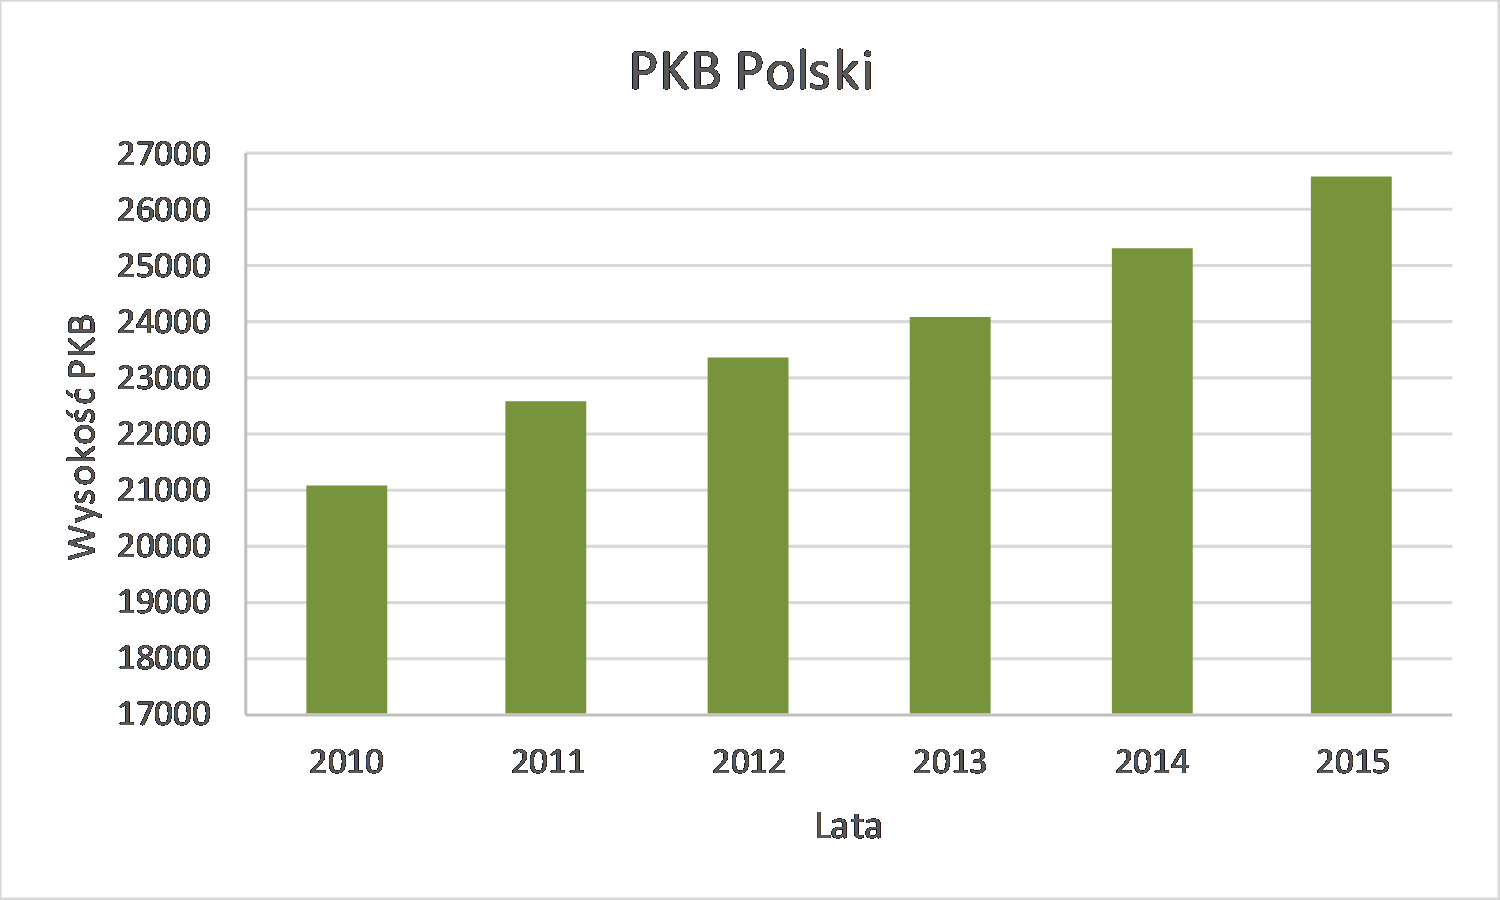
\includegraphics[width=1\textwidth]{ART_Rybka/pkb_polski.png} 
	\caption{Zmiana PKB \textit{per capita} według parytetu siły nabywczej mierzona dolarami międzynarodowymi.
		Źródło: opracowanie własne na podstawie
		\parencite{international_monetary_fund_world_2019a}.
%		\label{ref:RNDl3ypL6FseV}(International Monetary Fund, 2019a).
	}
	\label{fig1:ryb}
\end{figure}


%{\centering
%Rysunek 1. Zmiana PKB per capita według parytetu siły nabywczej mierzona dolarami międzynarodowymi%
%%Warto usunąć z~osi x lata ,,połówkowe'' bo to wygląda dziwacznie
%%nieznany
%%30 sierpnia 2019 15:45
%
%\par}
%
%{\centering
%[[[rysunek\_1]]]
%\par}
%
%źródło: opracowanie własne na podstawie \label{ref:RNDl3ypL6FseV}(International Monetary Fund, 2019a)

Jak wskazuje Rysunek \ref{fig1:ryb}, wartości PKB systematycznie rosły. Średni wzrost wskaźnika PKB w~latach 2010–2015 dla Polski
wynosi 1103,7 dolarów międzynarodowych. Najniższa wartość została odnotowana w~2010 r. Wynosi ona 21083,87 dolarów,
a~najwyższa pochodząca z~2015~r. to 26602,35. 

\begin{figure}[H]
	\centering
	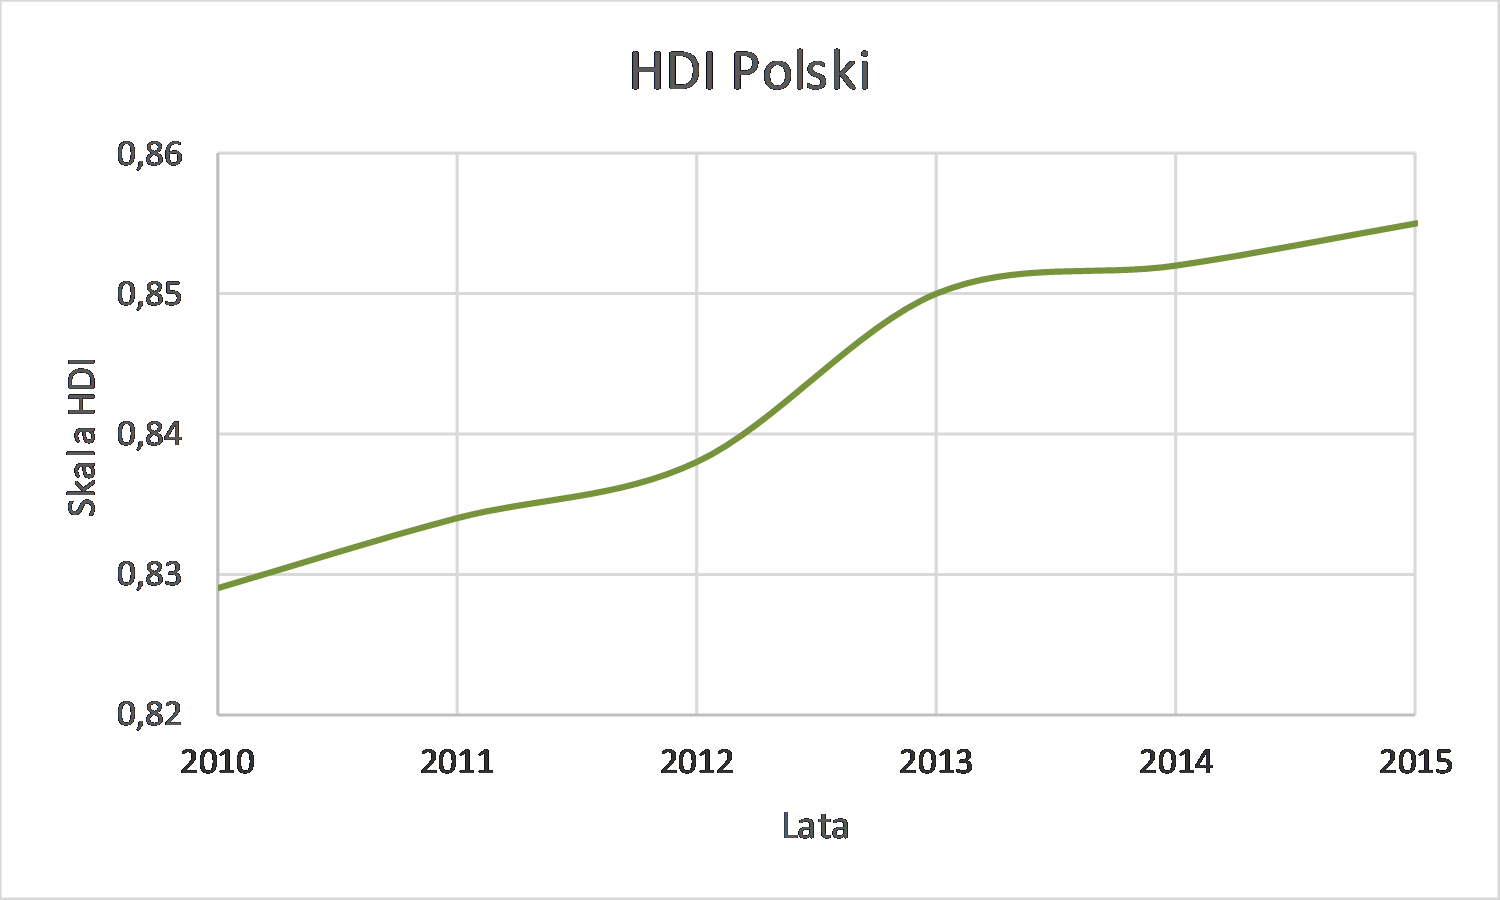
\includegraphics[width=1\textwidth]{ART_Rybka/hdi_polski.png} 
	\caption{Zmiana wartości HDI dla Polski.
		Źródło: opracowanie własne na podstawie
		\parencite{united_nations_development_programme_human_2019}.
%		\label{ref:RNDSuSEh9knxi}(United Nations Development Programme, 2019).
	}
	\label{fig2:ryb}
\end{figure}


%{\centering
%Rysunek 2. Zmiana wartości HDI dla Polski
%\par}
%
%{\centering
%[[[rysunek\_2]]]
%\par}
%
%źródło: opracowanie własne na podstawie \label{ref:RNDSuSEh9knxi}(United Nations Development Programme, 2019)

Wykres liniowy znajdujący się na Rysunku \ref{fig2:ryb} pokazuje zmiany zachodzące w~wartościach wskaźnika HDI. Przez cały okres
badania można zauważyć tendencję wzrostową. Największa zmiana wynosząca 0,012j. zachodzi pomiędzy 2012 a~2013 rokiem.
Średni wzrost wskaźnika HDI dla Polski to 0,0052j. przypadający na jeden rok badanego okresu. Różnica pomiędzy
wartością najwyższą oraz najniższą wynosi 0,03j.

\begin{figure}[H]
	\centering
	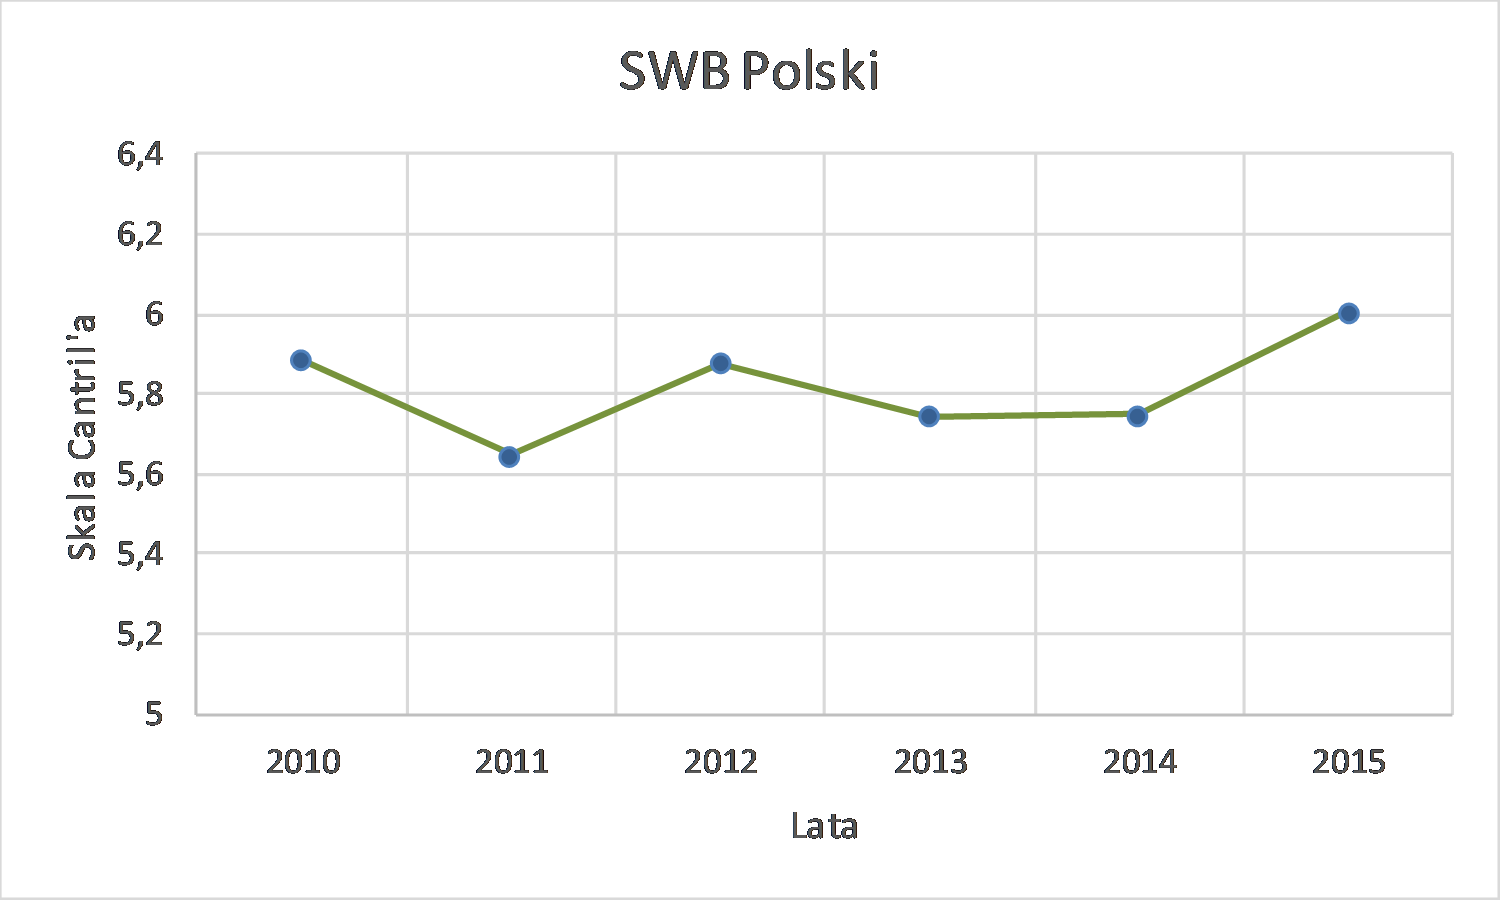
\includegraphics[width=1\textwidth]{ART_Rybka/swb_polski.png} 
	\caption{Zmiana wartości wskaźnika SWB Polski.
		Źródło: opracowanie własne na podstawie
		\parencite{noauthor_world_2018}.
%		\label{ref:RNDWHAJqDwCvX}(World Happiness Report, 2018).
	}
	\label{fig3:ryb}
\end{figure}


%{\centering
%Rysunek 3. Zmiana wartości wskaźnika SWB Polski
%\par}
%
%{\centering
%[[[rysunek\_3]]]
%\par}
%
%źródło: opracowanie własne na podstawie \label{ref:RNDWHAJqDwCvX}(World Happiness Report, 2018)

Na Rysunku \ref{fig3:ryb} została przedstawiona zmiana wartości wskaźnika SWB dla Polski. Jak można zaobserwować, wyniki skali
zmieniały się nieregularnie. W~latach 2010--2011 oraz 2012--2013 zauważalny jest spadek wartości wskaźnika, zaś w~latach
2011--2012 oraz 2013--2015 można spostrzec jego wzrost. Średni wzrost wskaźnika SWB wynosi 0,02j. Różnica pomiędzy
skrajnymi wartościami wynosi 0,36j.

Dla danych uzyskanych przez pomiar wskaźnikami PKB, HDI oraz SWB została przeprowadzona korelacja pomiędzy
poszczególnymi miernikami. Jej wyniki przedstawia poniższa tabela.

\captionsetup[table]{name=Tabela}
\begin{table}[H]
	\begin{tabularx}{\textwidth}{|Y|Y|}
		\hline
		\multicolumn{2}{|c|}{\bfseries Korelacja wskaźników dla Polski}\\\hline
		PKB z~SWB &
		0,32\\\hline
		PKB z~HDI &
		0,95\\\hline
		HDI z~SWB &
		0,21\\\hline
	\end{tabularx}
	
	\caption{Wartości związku pomiędzy poszczególnymi wskaźnikami dla Polski.
		Źródło: opracowanie własne na podstawie
		\parencite{international_monetary_fund_world_2019a,united_nations_development_programme_human_2019,noauthor_world_2018}.
%		\label{ref:RNDJaFcYZDBCr}(International Monetary Fund, 2019a; United Nations
%		Development Programme, 2019; World Happiness Report, 2018).
		}
	\label{tab3:ryb}
\end{table}


%{\centering
%Tabela 3 Wartości związku pomiędzy poszczególnymi wskaźnikami dla Polski
%\par}
%
%\begin{center}
%\tablefirsthead{}
%\tablehead{}
%\tabletail{}
%\tablelasttail{}
%\begin{supertabular}{|m{4.552cm}|m{4.55cm}|}
%\hline
%\multicolumn{2}{|m{9.302cm}|}{\centering{\bfseries Korelacja wskaźników dla Polski}}\\\hline
%\centering PKB z~SWB &
%\centering\arraybackslash 0,32\\\hline
%\centering PKB z~HDI &
%\centering\arraybackslash 0,95\\\hline
%\centering HDI z~SWB &
%\centering\arraybackslash 0,21\\\hline
%\end{supertabular}
%\end{center}
%źródło: opracowanie własne na podstawie \label{ref:RNDJaFcYZDBCr}(International Monetary Fund, 2019a; United Nations
%Development Programme, 2019; World Happiness Report, 2018)

%\enlargethispage{1\baselineskip}

Tabela \ref{tab3:ryb} przedstawiająca korelacje pomiędzy wartościami otrzymanymi przez mierniki wskazuje, że największy związek
zachodzi pomiędzy PKB oraz HDI, który wynosi 0,95 -- oznacza to, że korelacja między nimi jest bardzo silna. Tak
jak w~przypadku danych dla 103 państw, tak wysoki związek pomiędzy danymi może wynikać z~tego, że 1/3 wartości wskaźnika HDI
pozyskiwana jest z~danych dochodu narodowego brutto \textit{per capita}, który jest pochodną PKB. Związek pomiędzy
PKB a~wynikami SWB wyrażany współczynnikiem korelacji Pearsona wynosi 0,32. Jest to korelacja słaba, oznaczająca znikome
powiązanie pomiędzy tymi wskaźnikami. Najmniejszym związkiem statystycznym charakteryzują się mierniki HDI oraz SWB.
Wynosi on 0,21, co jest postrzegane jako bardzo słaba korelacja, lub praktycznie zerowy związek pomiędzy wartościami. 

Niska korelacja pomiędzy PKB i~SWB oraz HDI i~SWB może być związana z~tym, że Polacy nie utożsamiają swojego zadowolenia
z życia z~otrzymywanym dochodem. Według obliczeń przeprowadzonych na podstawie danych pochodzących z~World
Happiness Report wynika, że istnieje wysoka korelacja pomiędzy subiektywnym dobrobytem a~postrzeganym poziomem korupcji
na szczeblu rządowym i~samorządowym oraz w~sektorze prywatnym. Związek statystyczny pomiędzy SWB a~postrzeganym
poziomem korupcji wynosi -0,78, co jest korelacją silną oraz odwrotną. Oznacza to, że wraz ze spadkiem (wzrostem)
korupcji w~rządzie i~sektorze prywatnym wzrasta (spada) zadowolenie z~życia obywateli Polski. Średnia wyników
ankiet z~lat 2010--2015 mówi, że średnio aż 88\% ankietowanych uważa, że korupcja jest rozpowszechniona na szczeblu rządowym oraz
prywatnym
\parencite{noauthor_world_2018}.
%\label{ref:RNDcRU0ppjN4H}(World Happiness Report, 2018).
Zdaniem autora niska zależność pomiędzy PKB a~SWB
może być spowodowana tym, że Polacy mogą czuć się oszukiwani i~bezsilni wobec panujących układów korupcyjnych w~Polsce,
przez co wzrost (spadek) wynagrodzenia nie wiąże się ze wzrostem (spadkiem) poziomu subiektywnego dobrobytu.

%\enlargethispage{1\baselineskip}

Jak zostało przedstawione na
powyższych wykresach, wzrost wartości wskaźnika PKB \textit{per capita} według parytetu siły nabywczej mierzonego dolarami
amerykańskimi oznacza znikomy wzrost poziomu zadowolenia z~życia (SWB) wyrażonego przez Drabinę Cantrila. Najbardziej
skorelowane okazały się PKB oraz HDI. Związek pomiędzy nimi jest bardzo silny.
Wzrost jednego ze wskaźników powoduje wzrost średniej wartości drugiego wskaźnika. Korelacje pomiędzy miernikami
PKB i~SWB oraz HDI i~SWB są bardzo znikome. Może to być spowodowane pozaekonomicznymi czynnikami, które wpływają na
subiektywny dobrobyt mieszkańców Polski.

Drugim krajem przeprowadzonej analizy jest Grecja. To kraj południowo-wschodniej Europy. W~2002 r. Grecja
zrezygnowała ze swojej waluty na rzecz euro, w~2013 r. została zakwalifikowana do grupy krajów rozwijających się, co
stanowiło degradację z~kategorii krajów rozwiniętych. Był to pierwszy przypadek spadku z~grupy dla tego kraju
\parencite{international_monetary_fund_world_2019a}.
%\label{ref:RNDOaa1RXQDzx}(International Monetary Fund, 2019a).
W~2017 r. Grecję zamieszkiwało nieco ponad 10~mln mieszkańców,
w~tym samym roku odnotowano wysokość PKB rzędu 201 mld dolarów amerykańskich. PKB \textit{per capita} w~2017~r. osiągnęło zatem
wartość 18630 USD
\parencite{international_monetary_fund_world_2019b}.
%\label{ref:RNDRQRmi2Olaq}(International Monetary Fund, 2019b).
Kraj ten należy do dużej liczby
międzynarodowych organizacji, m.in. Paktu Północnoatlantyckiego od 1952 r., Unii Europejskiej od 1981 r., Organizacji
Narodów Zjednoczonych od 1945 r., oraz Organizacji Współpracy Gospodarczej i~Rozwoju od 1961 r. 

Grecja znajduje się na 28. miejscu rankingu 103 państw, w~którym pod uwagę brano PKB \textit{per capita} według parytetu siły
nabywczej liczonym dolarami międzynarodowymi. Według ranking wskaźnika rozwoju społecznego zajęła 21., a~pod względem
subiektywnego dobrobytu (SWB) znalazła się na 59. miejscu.

%\enlargethispage{1\baselineskip}

W poniższych tabelach zostanie przeprowadzona analiza wskaźnikowa dla Grecji.


\begin{table}[H]
	\begin{footnotesize}
		\begin{tabularx}{\textwidth}{|Y|Y|Y|Y|Y|Y|Y|}
			\hline
			\multicolumn{7}{|c|}{\bfseries Grecja}\\\hline
			~ &
			2010 &
			2011 &
			2012 &
			2013 &
			2014 &
			2015\\\hline
			{\bfseries SWB} &
			5,840 &
			5,372 &
			5,096 &
			4,720 &
			4,756 &
			5,623\\\hline
			{\bfseries PKB} &
			28961,80 &
			26850,25 &
			25433,14 &
			25194,26 &
			26017,86 &
			26389,71\\\hline
			{\bfseries HDI} &
			0,860 &
			0,858 &
			0,860 &
			0,862 &
			0,865 &
			0,866\\\hline
		\end{tabularx}
	\end{footnotesize}
	
	\caption{Zmiana wartości wskaźników Grecji.
		Źródło: oobliczenia własne na podstawie
		\parencite{international_monetary_fund_world_2019a,united_nations_development_programme_human_2019,noauthor_world_2018}.
%		\label{ref:RNDIkw0V6s683}(International Monetary Fund, 2019a; United Nations
%		Development Programme, 2019; World Happiness Report, 2018).
	}
	\label{tab4:ryb}
\end{table}

%{\centering
%Tabela 4 Zmiana wartości wskaźników Grecji
%\par}
%
%\begin{flushleft}
%\tablefirsthead{}
%\tablehead{}
%\tabletail{}
%\tablelasttail{}
%\begin{supertabular}{|m{3.6139998cm}|m{1.8179998cm}|m{1.977cm}|m{1.977cm}|m{1.9779999cm}|m{1.977cm}|m{1.984cm}|}
%\hline
%\multicolumn{7}{|m{16.525cm}|}{\centering{\bfseries Grecja}}\\\hline
%\centering{\bfseries ~} &
%\centering 2010 &
%\centering 2011 &
%\centering 2012 &
%\centering 2013 &
%\centering 2014 &
%\centering\arraybackslash 2015\\\hline
%\centering{\bfseries SWB} &
%\centering 5,840 &
%\centering 5,372 &
%\centering 5,096 &
%\centering 4,720 &
%\centering 4,756 &
%\centering\arraybackslash 5,623\\\hline
%\centering{\bfseries PKB} &
%\centering 28961,801 &
%\centering 26850,252 &
%\centering 25433,138 &
%\centering 25194,264 &
%\centering 26017,860 &
%\centering\arraybackslash 26389,706\\\hline
%\centering{\bfseries HDI} &
%\centering 0,860 &
%\centering 0,858 &
%\centering 0,860 &
%\centering 0,862 &
%\centering 0,865 &
%\centering\arraybackslash 0,866\\\hline
%\end{supertabular}
%\end{flushleft}
%źródło: obliczenia własne na podstawie \label{ref:RNDIkw0V6s683}(International Monetary Fund, 2019a; United Nations
%Development Programme, 2019; World Happiness Report, 2018)

Tabela \ref{tab4:ryb} pokazuje zmiany wartości wskaźników, jakie zachodziły na przestrzeni sześciu lat dla Grecji. Wskaźniki PKB oraz
SWB wskazują spadek swoich wartości w~latach od 2010 do 2013. Natomiast od 2013 do 2015 roku oba zaczęły wzrastać.
Wskaźnik rozwoju społecznego, oprócz roku 2011, w~którym zauważono spadek, wzrastał. Średnie wartości wskaźników to:

\begin{itemize}
\item SWB -- 5,234,
\item PKB -- 26474,504,
\item HDI -- 0,862.
\end{itemize}

%\enlargethispage{1\baselineskip}

\begin{figure}[H]
	\centering
	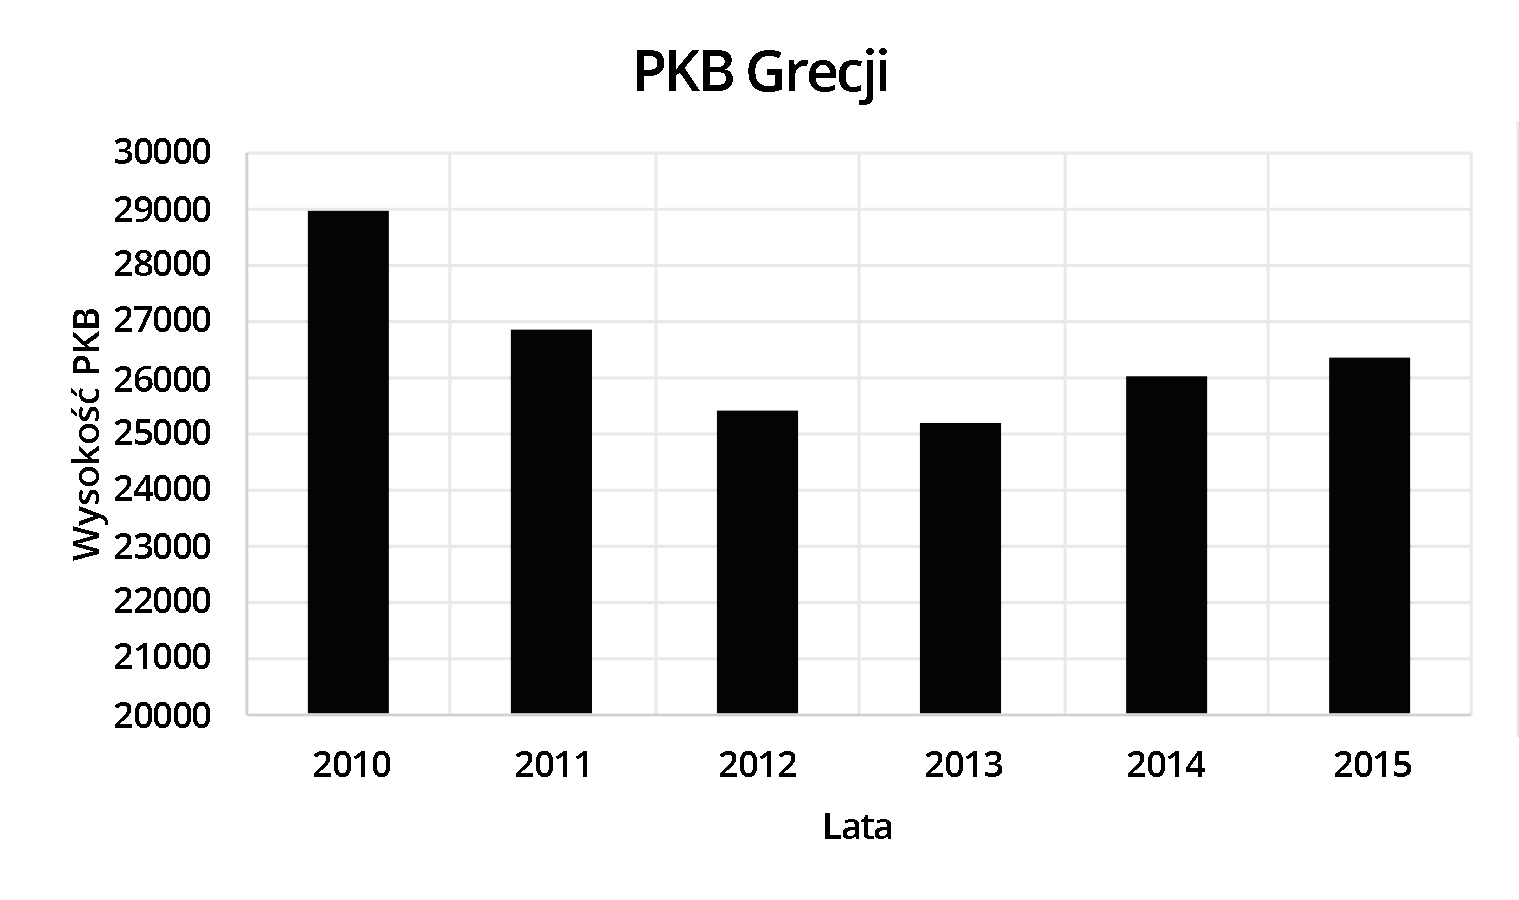
\includegraphics[width=1\textwidth]{ART_Rybka/pkb_grecji.png} 
	\caption{Zmiana PKB Grecji \textit{per capita} według parytetu siły nabywczej mierzona dolarami międzynarodowymi.
		Źródło: opracowanie własne na podstawie
		\parencite{international_monetary_fund_world_2019a}.
%		\label{ref:RND6yFA9J8VHO}(International Monetary Fund, 2019a).
	}
	\label{fig4:ryb}
\end{figure}

%{\centering
%Rysunek 4 Zmiana PKB per capita według parytetu siły nabywczej mierzona dolarami międzynarodowymi Grecji
%\par}
%
%{\centering
%[[[rysunek\_4]]]
%\par}
%
%źródło: opracowanie własne na podstawie \label{ref:RND6yFA9J8VHO}(International Monetary Fund, 2019a)

W zmianie wskaźnika PKB dla Grecji można zauważyć dwie tendencje. Jedna malejąca rozpoczynająca się w~2010 roku,
a kończąca się w~roku 2013, oraz wzrostowa, która początek ma w~2013~r. do 2015~r. PKB swoją największą wartość osiągnęło
w 2010 r., wyniosła ona 28961,801 dolarów międzynarodowych oraz najniższą w~2013~r. wynoszącą 25194,264. Średnia zmiana
wartości PKB wyniosła 514,419 dolarów. Różnica pomiędzy najwyższym i~najniższym odnotowanym PKB wynosi 3767,537 dolarów.


\begin{figure}[h]
	\centering
	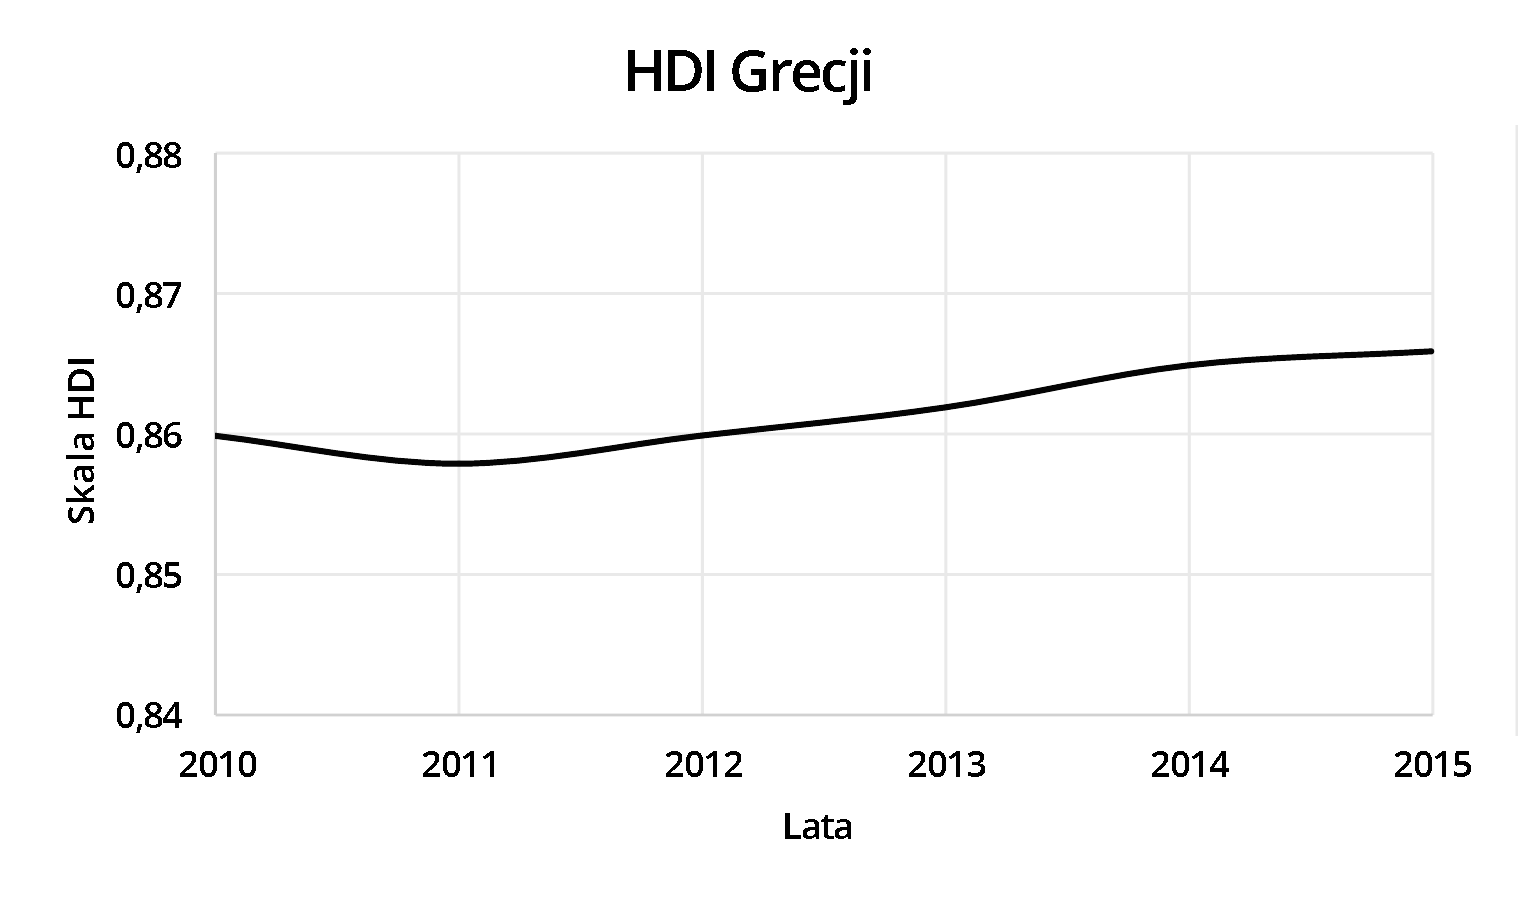
\includegraphics[width=1\textwidth]{ART_Rybka/hdi_grecji.png} 
	\caption{Zmiana wartości HDI Grecji.
		Źródło: opracowanie własne na podstawie
		\parencite{united_nations_development_programme_human_2019}.
%		\label{ref:RNDRvQ01uztWh}(United Nations Development Programme, 2019).
	}
	\label{fig5:ryb}
\end{figure}

%{\centering
%Rysunek 5 Zmiana wartości HDI Grecji
%\par}
%
%{\centering
%[[[rysunek\_5]]]
%\par}
%
%źródło: opracowanie własne na podstawie \label{ref:RNDRvQ01uztWh}(United Nations Development Programme, 2019)

Linia wskazująca zmiany HDI ulega niewielkim zmianom w~ciągu badanego okresu. Oprócz spadku w~roku 2011 tendencja
wskaźnika jest wzrastająca. Najwyższy punkt funkcja osiągnęła w~roku 2015 i~wyniosła 0,866, a~najniższy z~2011 roku
wyniósł 0,858. Różnica pomiędzy nimi wynosi 0,008. Średni wzrost wskaźnika HDI wyniósł 0,0012. 

\begin{figure}[h]
	\centering
	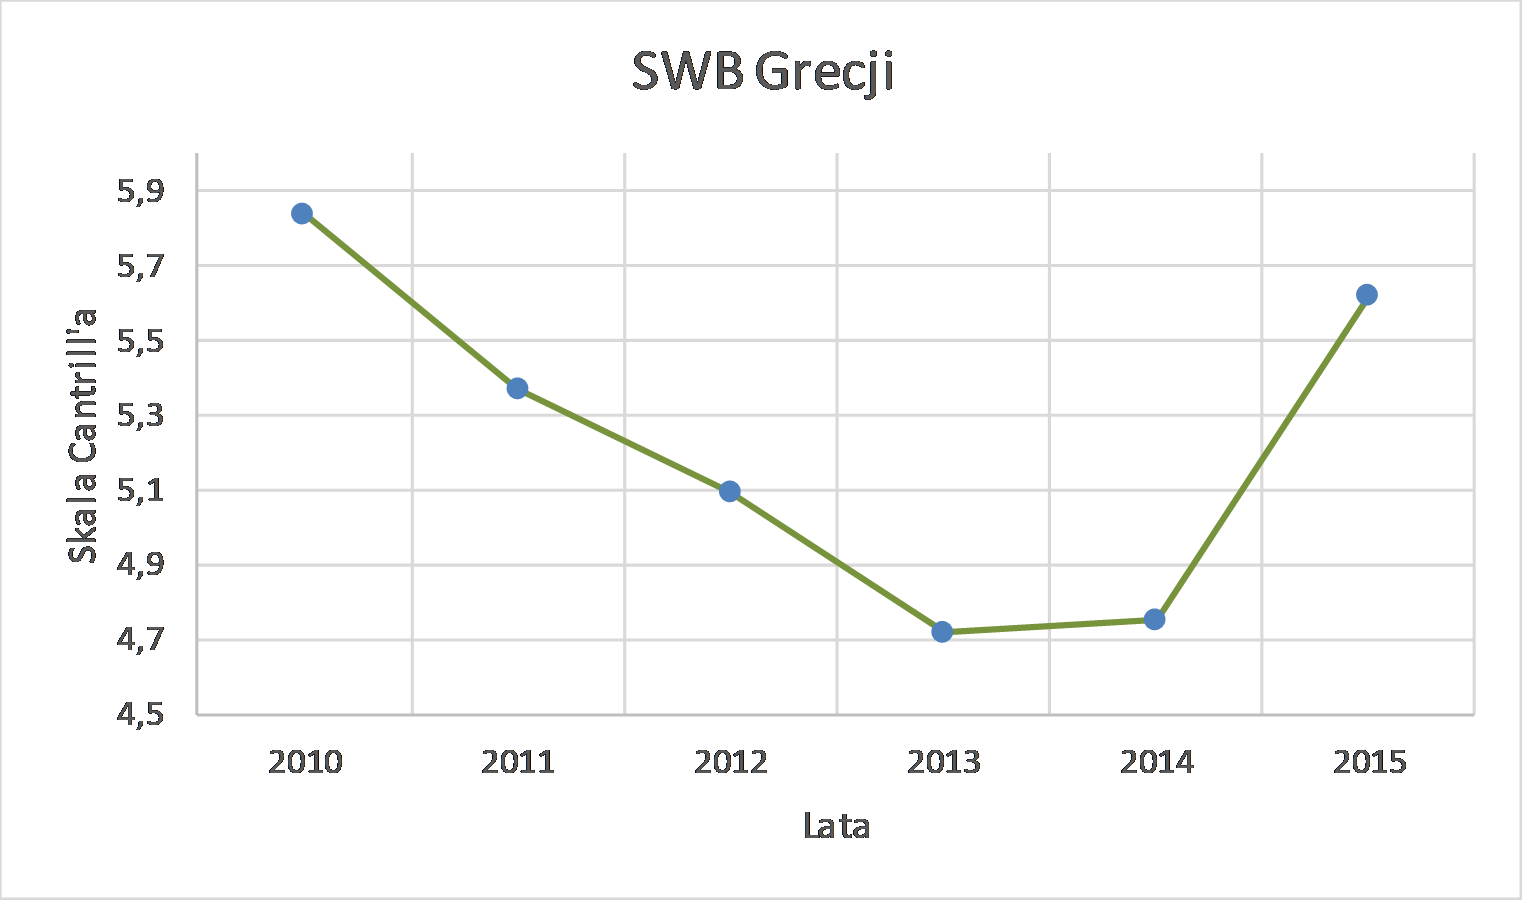
\includegraphics[width=1\textwidth]{ART_Rybka/swb_grecji.png} 
	\caption{Zmiana wartości SWB Grecji.
		Źródło: opracowanie własne na podstawie
		\parencite{noauthor_world_2018}.
%		\label{ref:RNDB7u1qcEsSx}(World Happiness Report, 2018).
	}
	\label{fig6:ryb}
\end{figure}


%{\centering
%Rysunek 6 Zmiana wartości SWB Grecji
%\par}
%
%{\centering
%[[[rysunek\_6]]]
%\par}
%
%źródło: opracowanie własne na podstawie \label{ref:RNDB7u1qcEsSx}(World Happiness Report, 2018)

Wykres łączący punkty wartości SWB wskazuje podział na dwa okresy: spadku oraz wzrostu. Pierwszy z~nich zauważalny jest
na przestrzeni lat 2010--2013. Drugi to okres wzrostu występujący w~latach 2013--2015. Najwyższy punkt wykresu przypada
na rok 2010 i~wynosi 5,84. Najniższy został odnotowany w~roku 2013, który wskazuje na wartość 4,72. Różnica pomiędzy
najwyższym i~najniższym punktem wynosi 1,12.  Największy wzrost wartości został odnotowany pomiędzy 2014 i~2015 rokiem
i~wyniósł 0,866. Średni spadek wartości SWB Grecji w~badanym okresie wyniósł 0,043.

\captionsetup[table]{name=Tabela}
\begin{table}[H]
	\begin{tabularx}{\textwidth}{|Y|Y|}
		\hline
		\multicolumn{2}{|c|}{\bfseries Korelacja wskaźników dla Grecji}\\\hline
		PKB z~SWB &
		0,82\\\hline
		PKB z~HDI &
		-0,29\\\hline
		HDI z~SWB &
		{}-0,19\\\hline
	\end{tabularx}
	
	\caption{Wartości związku pomiędzy wskaźnikami Grecji.
		Źródło: obliczenia własne na podstawie
		\parencite{international_monetary_fund_world_2019a,united_nations_development_programme_human_2019,noauthor_world_2018}.
%		\label{ref:RNDUidV4ndp13}(International Monetary Fund, 2019a; United Nations
%		Development Programme, 2019; World Happiness Report, 2018).
	}
	\label{tab5:ryb}
\end{table}


%{\centering
%Tabela 5 Wartości związku pomiędzy wskaźnikami Grecji
%\par}
%
%\begin{center}
%\tablefirsthead{}
%\tablehead{}
%\tabletail{}
%\tablelasttail{}
%\begin{supertabular}{|m{5.3cm}|m{3.441cm}|}
%\hline
%\multicolumn{2}{|m{8.941cm}|}{\centering Grecja}\\\hline
%\centering PKB z~SWB &
%\centering\arraybackslash 0,82\\\hline
%\centering PKB z~HDI &
%\centering\arraybackslash {}-0,29\\\hline
%\centering HDI z~SWB &
%\centering\arraybackslash {}-0,19\\\hline
%\end{supertabular}
%\end{center}
%źródło: obliczenia własne na podstawie \label{ref:RNDUidV4ndp13}(International Monetary Fund, 2019a; United Nations
%Development Programme, 2019; World Happiness Report, 2018)

Tabela \ref{tab5:ryb} wskazuje na wartości związku pomiędzy poszczególnymi wskaźnikami. Największa korelacja zachodzi pomiędzy
wskaźnikami PKB oraz SWB, która wynosi 0,82. Jest to związek silny, a~przez niektóre źródła uznawany za bardzo silny.
Wynika z~niego, że wraz ze wzrostem wartości jednego wskaźnika następuje wzrost średniej wartości drugiego. Najniższą,
ujemną korelacją odznaczyły się mierniki HDI oraz SWB, która wyniosła -0,19. Jest to słaby związek pomiędzy danymi.
Podobną sytuację można zauważyć pomiędzy wskaźnikami PKB oraz HDI, dla której korelacja wyniosła -0,29. Dla obu
wartości wzrost (spadek) jednego wskaźnika oznaczał spadek (wzrost) drugiego. 

Tym, co najsilniej przykuwa uwagę, jest zadziwiająco wysoka korelacja pomiędzy PKB oraz SWB. Wartość
związku pomiędzy nimi jest silna. Oznacza to, że wzrost (spadek) zamożności obywateli
Grecji wiązał się ze wzrostem (spadkiem) ich subiektywnego dobrobytu. Taka sytuacja może być spowodowana kryzysem
gospodarczym, który panuje w~Grecji, oraz z~nastrojami mieszkańców. Jak można zauważyć analizując wykresy PKB oraz SWB,
oba wskaźniki odnotowały spadki i~wzrosty dokładnie w~tych samych latach. Także skrajne wartości tych wskaźników
przypadały na ten sam okres. Zadziwiająca jest także sytuacja mająca miejsce pomiędzy wskaźnikami PKB oraz HDI. Nie
tylko korelacja między nimi jest słaba, to na dodatek jest ona odwrotna, co oznacza, że wraz ze wzrostem (spadkiem)
wartości jednego ze wskaźników związany był spadek (wzrost) wartości drugiego wskaźnika. Jest to sytuacja nietypowa,
ponieważ dochód narodowy brutto \textit{per capita} będący pochodną wskaźnika PKB jest częścią HDI. Najniższa korelacja
wystąpiła pomiędzy wskaźnikami HDI oraz SWB, która odznaczała się słabym związkiem. 

Autor pracy przeprowadził obliczenia dotyczące korelacji pomiędzy zadowoleniem z~życia, a~poziomem wskaźnika Giniego.
Wynika z~nich, że istnieje bardzo silny związek pomiędzy tymi dwiema sferami, ponieważ wskaźnik korelacji Pearsona
wynosi aż -0,88. Jest to korelacja odwrotna, z~której wynika, że wraz ze wzrostem (spadkiem) nierówności dochodowych
spada (wzrasta) subiektywne zadowolenie z~życia Greków. Ta sytuacja może być związana z~panującym w~tych
latach w~Grecji kryzysem gospodarczym. Druga wysoka korelacja, która wynosi 0,74, jest zauważalna pomiędzy subiektywnym
dobrobytem a~wolnością podejmowania życiowych decyzji
\parencite{noauthor_world_2018}.
%\label{ref:RNDaAxMI6IUZa}(World Happiness Report, 2018).
Oznacza
to, że dla Greków ważną kwestią wpływającą na ich subiektywne zadowolenie może być wolność w~podejmowaniu decyzji
związanych z~własnym życiem.

Powyższe badania potwierdzają hipotezę, która mówi, że wzrost dobrobytu ekonomicznego nie zawsze wiąże się
ze wzrostem subiektywnego dobrobytu. Obliczenia dotyczące wszystkich 103. państw pokazują także, że największy związek
występuje pomiędzy dobrobytem ekonomicznym oraz ogólnym. Hipoteza zakładała także występowanie większego związku
pomiędzy dobrobytem ogólnym i~subiektywnym niż dobrobytem ogólnym oraz ekonomicznym, lecz przeprowadzone obliczenia jej
zaprzeczają.

\section{Zakończenie}
Tematem przewodnim pracy było wskazanie różnorodności teorii dobrobytu, przedstawienie wskaźników
umożliwiających ich pomiar oraz analiza zależności statystycznych pomiędzy trzema rodzajami dobrobytu (ekonomicznym,
ogólnym oraz subiektywnym) obliczonymi przez wskaźniki PKB, HDI oraz SWB. Z~opracowania wynika, że istnieje bardzo
szeroka gama teorii oraz koncepcji związanych z~dobrobytem, które czasami się wykluczają. Czytelnik może także się
dowiedzieć, że pod jednym hasłem -- dobrobyt -- w~polskiej literaturze kryją się dwa, różne od siebie zjawiska, czyli
dobrobyt ekonomiczny (\textit{welfare)} oraz dobrobyt ogólny (\textit{well-being}). Najważniejszym wnioskiem
płynącym z~opracowania jest to, że związki pomiędzy dobrobytem ekonomicznym a~ogólnym reprezentowanym kolejno przez PKB
oraz HDI są bardzo silne, a~związki pomiędzy dobrobytem ekonomicznym i~subiektywnym zadowoleniem z~życia (SWB
obliczonym za pomocą drabiny Cantrila) oraz dobrobytem ogólnym i~subiektywnym są znikome. Jednak jak pokazują analizy
szczegółowe przeprowadzone na dwóch krajach Unii Europejskiej -- Polsce oraz Grecji -- związki te nie zawsze są silne. 

Przeprowadzone badanie wskazuje jedynie na zależność pomiędzy wartościami dobrobytu poszczególnych krajów.
Związek także nie uwzględnia zależności przyczynowej, tylko obrazuje, że dane zjawiska zachodzą obok
siebie. Ukazuje to jedynie, że dane zjawiska mają miejsce, lecz badania nie wskazują konkretnie przyczyn ich
występowania. Aby wytłumaczyć zaistnienie pewnych zależności, można prześledzić sytuację społeczno-ekonomiczną
mieszkańców danych państw, w~celu poznania przyczyn. 

Autor pracy uważa, że przyszłe badania nad zjawiskiem dobrobytu powinny być prowadzone we współpracy z~przedstawicielami
wielu dziedzin naukowych w~celu zbadania aspektów mogących wpływać na dobrobyt. W~szczególności rekomenduje współpracę
nauk psychologicznych z~ekonomicznymi w~celu dokładnego zbadania dobrobytu subiektywnego.

\end{artplenv}\label{rybka-stop}













%\sekcja{Z prac Komisji Filozofii Nauk PAU}{Proceedings of the PAU Commission\\\ on the Philosophy of Science}

%\input{PAU_Lamza/Lamza.tex}


%\addtocontents{toc}{\protect\pagebreak}



\sekcja{Recenzje}{Book reviews}

\begin{recengenv}{Marcin Gorazda}
	{Believable world of economic models}
	{Believable world of economic models}
	{Łukasz Hardt, \textit{Economics Without Laws: Towards a New Philosophy of Economics}, Palgrave Macmillan, Cham, 2017,
		pp.220.}
	
	



\subsubsection{Introduction}
Philosophy of economics is a young discipline, especially in Poland, which is still looking for its proper place within
the scientific world and its definition. What has been contemplated so far under this brand is a mixture of the
methodology of economics, the ontology of economic phenomena and ethical commitments in economics. Hardt’s book
subscribes itself to this club and constitutes a fascinating example of such an analysis. The book is outstanding for
many reasons (which are developed further below), but one must be emphasized at the very beginning. As far as the
reviewer is aware it is the first book by Polish economist and philosopher in the field of philosophy of economics
published in English by the distinguished scientific publisher. Therefore, regardless of some minor reservations below,
Łukasz Hardt definitely did a great a job as a representative of Polish thinkers. 

Hardt’s book focuses mainly on ontological and methodological issues in economics, especially the part economic laws and
economic models play in the explanation of economic phenomena. As economists usually present their ideas in the form of
various models, their methodological and ontological status is definitely of utmost importance. However, it needs to be
underlined that the analysis is done from the specific point of view, namely scientific realism which is in opposition
to scientific constructivism or instrumentalism and which still seems to dominate the contemporary philosophy of
science.  Even if the author in some places declares that he intends to find the third way somewhere in between, his
initial stance, used terminology and style of reasoning constitutes a clear hallmark and sometimes a burden, not easy
to be neglected. 

There is a general idea in the book’s background, which I believe is shared commonly by the philosophers of economics,
that there seems to be a crucial distinction between the exactness of the so-called natural sciences and inexactness of
the social sciences, economics including. On the phenomenal level, the distinction may be observed by the apparent
inability of economics to formulate reliable predictions. For some thinkers, if the specific science is unable to
predict future outcomes, it undermines its scientific character. And as those predictions are usually formulated based
on the past regularities which are then reformulated into the universal laws of nature, the natural question is about
the status of those laws. Is it possible to practice any science without the concept of scientific laws? What would be
the construction of scientific theory if there be no laws and how such a theory may explain? The book is a courageous
attempt at answering those hard philosophical questions. 

Briefly, Hardt claims that it is not about laws in economics but about tendencies, models based on \textit{ceteris
normalibus} assumptions, mechanisms, believable worlds which are never entirely true but for some reasons might be
considered believable and therefore may have certain explanatory power and be informative for policymakers.

\enlargethispage{-1\baselineskip}

Hardt’s account is a strong case against law-centrism in science and especially in economics as well as against
dogmatism and fundamentalism. According to him, the economists’ efforts concentrate and should concentrate on models’
construction and their further exploration and those efforts may eventually bring them about the reliable insight into
the essentials of the modelled economic realm. 

\subsubsection{The composition and the content of the book}
Reading the book, one has to acknowledge that its composition is compliant to its content. The chapters are logically
sequenced what makes the line of reasoning transparent and comprehensible. The introduction gives us an overview of the
book’s content, and brief information about the main theses defended. The first chapter is an in-depth review of the
thoughts of four well known classical economists on the nature of economic law. From this perspective, Hardt
scrutinises the works of Adam Smith, David Ricardo, John Stuart Mill and Alfred Marshall, and this scrutiny is itself
an achievement worth reading. There were thousands of pages written on those worldly philosophers, but I do not recall
myself any attempt at reconstructing their methodological and ontological views on the economic laws (except Mill whose
concept of tendencies is broadly discussed). However, the conclusions of that chapter are in the end, a bit untoward.
As we learn from the introduction and the book’s title, Hardt is trying to persuade the reader that this law-centrism
in economics was declining throughout the centuries. So I would expect that the chosen thinkers were drifting from the
concept of universal economic laws toward the theoretical models. It is not precisely the case. Even Smith, who as
Hardt admits, used the idea of universal laws at least on the sematic level is presented like the contemporary
theorist, whose references to the universal laws are due to his fresh, underdeveloped awareness of the scientific
methodology.  We read:


\begin{myquoterev}
	[\mydots] Smith’s claims suggesting the existence of universal economic laws are a testimony of his desire to build a
deductive economic theory and his more cautious assertions about the working of the real markets expresses his
empirical orientation
\parencite[p.30]{hardt_economics_2017}.
% \label{ref:RNDwvxc7jkftR}(Hardt, 2017, p.30).
\end{myquoterev}
And further

\begin{myquoterev}
[\mydots] it is certain that his economic laws are not universal natural laws and their nature is more complicated
\parencite[p.31]{hardt_economics_2017}.
%\label{ref:RNDmAffQKsxYM}(Hardt, 2017, p.31).
\end{myquoterev}

\enlargethispage{-.5\baselineskip}

In Hardt’s interpretation, Ricardo is an abstract model’s constructor, Mill, an author of the concept of laws as
tendencies and Marshal is a denialist of the ``possibility of all-encompassing knowledge about the economic phenomena''.
He concludes that ``classical economists, together with Marshall, kept their conclusions regarding economic reality
separated from their purely theoretical claims''. In the light of the next chapter, ``The Demise of Laws in Economics'' it
makes the whole story more complicated. The reader may be puzzled. If even the most classical economists were not the
proponents of ``universal regularities that are omnitemporally and omnispatially true characterised by a high level of
necessity'' so who was? The answer is offered in the next chapter, which is supposed firstly to ``sketch the history of
the process of the demise of law-centrism in the philosophy of science'' and secondly to present other approaches to
scientific explanations which do not refer to the scientific laws with special emphasise of \textit{ceteris paribus} laws. In
this chapter, we also find an astonishing commentary on natural law tradition in economics. The author finds two
sources of law-centrism. The first is David Hume and his concept of causation as a regular concomitance between events
and their effects. The second is the neo-positivism, and especially Hempel’s account of explanation in science wherein
the law of nature is a necessary component of sound explanatory reasoning. However, the central part of the chapter
includes the discussion with those ``traditional'' accounts and presentation of other views, the author’s including.
Here, after remarks on models, we learn what the idea of the science without law means:

\begin{myquoterev}
It is not to erase the notion of laws from the fabric of science, but rather to define their role in a very specific
way, precisely, as statements being always true only in models used in their construction
\parencite[p.78]{hardt_economics_2017}.
%\label{ref:RND2lliVQaVuL}(Hardt, 2017, p.78).
\end{myquoterev}

Models in science and specifically in economics are crucial not only because they are the modern way of practising
economics but mainly because models are theory-creators and in them the capacities manifest themselves. Models,
however, have certain constraints which can be translated into the CP-laws, which are nevertheless explanatory and are
expected to survive the transition to the world. 

Chapter fourth is dedicated to the causal explanations in economics, and it constitutes a pretty good, though a
necessarily subjective summary of what remarkable has been written on the subject matter so far. Again the necessary
point of reference is the Humean concept of causation, which is outlined but mostly criticised. Undoubtedly he gave
rise to the set of regularity theories of causation, and probability view, which are still prevalent in contemporary
economics, both being discussed in the consecutive sections. The special place is reserved for Nancy Cartwright’s
account of capacities
\parencite*{cartwright_dappled_1999},
%\label{ref:RNDXu10TYyjs3}(Cartwright, 1999),
which is understandable as the author declares that,
although ``\mydots it seems that finding the appropriate theory of causation is impossible and we should accept the coexistence
of various philosophies of causation [\mydots] it does not mean that all of them are equally valid—for me the most
promising ones are approaches that are metaphysically rich; for example the Cartwright’s approach''
\parencite[p.118]{hardt_economics_2017}.
%\label{ref:RNDin7H4veSHJ}(Hardt, 2017, p.118).
In the last sections, we find an overview of the interventionist account
and causation in econometrics. 

Chapter five is probably the most important in the book, as it presents the author’s original idea of economic models as
believable worlds. This concept is so peculiar that it requires more in-depth analysis provided in the sperate section
below.

%\enlargethispage{-.1\baselineskip}

In the last chapter, the so-called distinctively mathematical explanations are discussed as the possible new sort of
explanation in economics, which seems to be already applied but is also promising for the future. The statement that
mathematic dominates economics is trivial. It is extensively used in many different fields. The focus in the chapter is
however on the mathematical explanation in the ``external'' sense, where according to the author mathematics is not only
the tool of deduction besides the causes and scientific laws but it explains by itself. It constitutes the decisive
element of explanation. The concept is not easy to be comprehended, so Hardt gives us examples. Thomas Schelling’s
checkboard model of segregation is considered to be a distinctively mathematical explanation while Hal Varian’s model
of sale and price distortion is not. The main difference is that in Schelling’s model there is no causal inference and
no references to the economic laws, and the empirical interpretation (or application) is given ex-post, while in
Varian’s model the causal chain is fundamental. The conclusion is that the causal–mechanistic explanation in economics
is more typical, while Schelling’s case is rather exceptional. 

\subsubsection{Some critical remarks on laws and models}
Although the book presents an interesting position in the contemporary philosophy of economics, and its composition,
comprehensive approach to the discussed topics and references to ideas of well-known economists and philosophers make
it excellent reading for anyone interested in the subject matter, it has certain shortcomings. They lie mainly in those
parts of the book which constitute the core of Hardt’s account and which are therefore the most challenging.  

Let me start from the leading thesis that the concept of economics founded on scientific laws is obsolete and no longer
sustainable. Scientific laws are not in the centre of economic explanation. This leading thesis makes sense only in
light of the very peculiar understanding of scientific laws, namely ``universal regularities that are omnitemporally and
omnispatially true characterised by a high level of necessity''. Although such a definition is quite often a point of
departure for further discussion, it is usually considered to be a counterexample for presenting the main problems of
philosophy of science and thus naïve. I could hardly name a philosopher who really believes that any scientific law
meets this characteristic. Apparently, after reading the excellent historical chapter of Hardt’s book, I guess that he
could hardly name such an economist too. Is Hume the right candidate? I doubt. His concept of causation based on
temporal and spatial contiguity and especially his uniformity principle may resemble Hardt’s definition of the law of
nature, but one has to remember that both are constructs of our mind,  customs, beliefs that the future will be like the
past. Empiricist has nothing to say on the ontology of those phenomena, and the causal chain is always hypothetical as
based on fallible features of our mind
\parencite{hume_treatise_2000}.
%\label{ref:RNDgCfw5zFZf9}(Hume, 2000).
Better candidates seem to be the
neo-positivists like Hempel
\parencite{hempel_studies_1948}
%\label{ref:RNDgDJCOUayAj}(Hempel and Oppenheim, 1948)
and Rudolf Carnap
\parencite*{carnap_logical_1967}.
%\label{ref:RNDnuhNCZiVns}(1967).
They might have believed in the universal laws of science and its cognizability, and
at least they used this concept in the explanatory reasoning, and they were trying to work out the logic of induction
which could provide the scientist with the method of sound reasoning from the observable repetitive phenomena to the
universal inductive generalisation. The problem is that they failed, remaining an interesting counterexample rather for
contemporary philosophy of science and moreover, they have never dedicated their work to social sciences like
economics, and their respective impact on this field was rather weak. Hardt knows it. In the chapter devoted to
scientific laws, most of the discussion is about the ideas which were trying to soften this demanding and impractical
definition of scientific law. On the other hand, if we relax the definition of laws of nature and acknowledge that they
are certain generalisations of observed regularities strongly dependent on assumed or observed constraints and context,
then the leading thesis seems unproven. 

A few words must be dedicated to Hardt’s concept of scientific models. It is not clear what models for Hardt are, but it
seems that he rejects the mathematical approach, wherein models are considered to be an interpretation of particular
language expressed with the use of predicates, constants, variables, functions and relations
\parencite{margaris_first_1990}.
%\label{ref:RNDd0TBcMbEPL}(Margaris, 1990).
It reads:

\begin{myquoterev}
[\mydots] logical positivism gave rise to the syntactic view of theories according to which a given theory is a set of
sentences in an axiomatized system of first order logic. In such an approach, there should be no role for other
consituents of science, including models . [\mydots] according to the syntactic view of theories, ‘a model is just a system
of semantic rules that interpret the abstract calculus and the study of a model amounts to scrutinizing the semantics
of a scientific language’. So, models are not independent entities, since they are largely defined by theories. No
theories (including laws of these theories), no models
\parencite[p.71]{hardt_economics_2017}.
%\label{ref:RNDeKOoqy83Yq}(Hardt, 2017, p.71).
\end{myquoterev}

It is a pity. Both first-order logic and models defined therein constitute an useful pattern to which we can always
refer. Rejecting this pattern may be the reason why Hardt perceives the difference between above criticised semantic
approach and his account. In the same section below, he quotes Ronald Giere and adds his comment which may give us a hint of
that:

\begin{myquoterev}
What have traditionally been interpreted as laws of nature thus turns to be merely statements describing the behaviour
of theoretical models''. So here the focus is on models but not as systems of semantics rules (syntactic views on
theories) but rather as being constitutive parts of theories. No models, no theories one could say (in syntactic
approach it is the other way round)
\parencite[p.72]{hardt_economics_2017}.
%\label{ref:RNDECtyz7BF9H}(Hardt, 2017, p.72).
\end{myquoterev}

This idea that models are instruments of theory creation returns in other chapters and sections of the book and has its
source in detachment of models from its mathematical pattern. It makes him forget that the main feature of the function
of interpretation is to preserve the truth value of sentences and that the function is reflexive. So these two
statements, no model, no theory and no theory, no model are rather equivalent. It would not be equivalent only in case
the author determined the features of the interpretation function in a way declining from its mathematical pattern. He
probably did, but without the reference to the pattern, it is not clear what was his intention. I deduce it from the
fact that in his account the isomorphism is gradable and respectively the truth value of the sentences in the model and
modelled domain are not entirely preserved after the ``transition''. Surprisingly within these sentences, we also find
laws of nature, and they play a remarkable part as we learn that  ``models are specified by laws''.  Therefore he claims
that science without laws ``is not to erase the notion of laws from the fabric of science, but rather to define their
role in a very specific way, precisely as statements being always true in models used in their construction''.  If this
interpretation is correct, so having in mind the fact that no one supports a very restrictive definition of a
scientific law, we have to conclude that that the concept of laws has not been erased from the fabric of science, as
they still constitute the foundation of a theories and models, and the perverse title of the book is a rhetorical trick
rather than an expression of a serious claim. Moreover, if the level of model’s isomorphism is gradable what means that
depending on this level some sentences in a model are true and some false, and if among those statements are scientific
laws, how is it possible that they are always true in a model? Either they are tautologies true by assumptions and
applied inference rules or we have another test of this truth value. If the latter is the case, we should find an
answer in the chapter on models as believable worlds. They are indeed supposed to include the test of the truth value.
Hardt’s proposal is worth quoting:

\begin{myquoterev}
It was shown that models explain by producing theoretical insights (laws) that are always true within models but they
are just beliefs if claimed to accurately describe the real world. Thus such beliefs are more credible if the target is
close enough to the model’s structure
\parencite[p.161]{hardt_economics_2017}.
%\label{ref:RND9hoO4b7tbR}(Hardt, 2017, p.161).
\end{myquoterev}

In his concept of models as believable worlds, the important element is a ``theoretical insight'' produced by the model.
Laws are part of that insight, and they are, again true within a model. Here it is more expressly stated that they are
``true'' as they are either assumed or deduced according to the assumed rules of inference. If they are not, the model is
inconsistent and useless. But they are also beliefs about the real world, and credibility of those beliefs is gradable.
So instead of external test for truth value, we need a test for the level of credibility. We need the reliable (or
workable) criteria; otherwise models with outstanding theoretical insight, inherently true (consistent) might be
entirely detached from any economic realm and at most explains the meanders of the researcher’s mind. Here the
criterium is the closeness of the target to the model’s structure. So, how to assess the ``closeness''? In the chapter,
we encounter several attempts at clarification this term or its replacements, like ``similarity''. We learn that to be a
believable world, the model must meet the requirement of the mechanism in James Woodward’s terms
\parencite{woodward_what_2002}.
%\label{ref:RNDnSeS1zWnlr}(Woodward, 2002).
So any model which is based on, e.g. data analysis but do not present any
mechanistic interpretation is by definition excluded. We also learn that it must refer to the ``essential explaining
items (including mechanism)'', but we do not know how to distinguish between essentials and non-essentials. But the
problem is correctly formulated. Hardt asks, what if we have multiple models fulfilling the above conditions? Which one
is closer or more similar to the target? And he proposes an answer: ``\mydots one must check as to what extent the theories
brought upon by models survive the transition from the world of the model to the real world'', period. Further reading
does not give us any further insight into the puzzling process of ``transition''. In reference to the exemplary model of
price distortion by Varian, Hardt only remarks: ``\mydots what is needed is a systematic empirical investigation into the
applicability of the model’s theoretical claims to a particular domain''
\parencite[p.154]{hardt_economics_2017}.
%\label{ref:RNDVQCseTAFgx}(Hardt, 2017, p.154).
I would say that the job is at least unfinished. The crucial element of his account, the criteria of various model
discriminations are not explained. The problem is shifted step by step to the consecutive, vogue terms: similarity,
closeness, transition survival. 

\subsubsection{Is the book worth reading? }
Although I could not resist myself from the above critical remarks, I still maintain that the book is worth reading, for
at least three reasons:

\begin{enumerate}
\item It is very informative. The reader can learn a lot about various ideas of philosophers of science (especially
economics) mostly from the realistic camp and those ideas are presented clearly and comprehensively. They are supported
with numerous, well-chosen examples from economics. So not only economists can learn some philosophy but also
philosophers can learn some economics. Anyway, the author is an economist in the first place. 
\item It is inspiring. The fact that I allow myself to present the above critical remarks is a visible sign that Hardt’s
ideas make us think about them thoroughly and sometimes makes us reconsider our position or become more aware of it. 
\item It is a good and pleasant reading, demanding in certain sections but definitely not dull. 
\end{enumerate}


\autorrec{Marcin Gorazda}

\subsubsection{Bibliography}\nopagebreak[4]
\end{recengenv}


\begin{recplenv}{Joanna Dzionek-Kozłowska}
	{Metarefleksje o~makroekonomii i~polityce makroekonomicznej}
	{Metarefleksje o~makroekonomii i~polityce makroekonomicznej}
	{Tomasz Kwarciński, Agnieszka Wincewicz-Price (red.), \textit{Metaekonomia II. Zagadnienia z~filozofii makroekonomii},
		Kraków, Copernicus Center Press 2019, ss. \ldots}





Zagadnienia metaekonomiczne to kwestie tak fundamentalne dla nauk ekonomicznych, że częstokroć jawią się one osobom
parającym się uprawianiem ekonomii jako zbyt oczywiste, przez co niewarte szczególnej uwagi, albo przeciwnie -- na tyle
trudno uchwytne, że w~oczach wielu podważa to zasadność wysiłku włożonego w~pogłębioną nad nimi refleksję. Nieliczni
teoretycy zastanawiają się, czym w~istocie są konstruowane przez nich modele makroekonomiczne. Jaki jest lub powinien
być związek modeli z~realnym życiem gospodarczym? Czy makroekonomia -- tworzone na jej gruncie
modele i~koncepcje -- \mbox{mogą/będą} kiedykolwiek
mogły dostarczyć nam jednoznacznych wskazówek pod adresem polityki gospodarczej? Nieco częściej,
zwłaszcza w~okresach pogorszenia koniunktury, daje się słyszeć pytanie o~to, czy w~ogóle zasadne jest pokładanie wiary
w~teoriach makroekonomicznych jako środkiem ochrony przed recesją, bezrobociem, inflacją, obniżeniem dobrobytu i~innymi
bolączkami o~charakterze ekonomicznym. Ujmując rzecz z~jeszcze innej perspektywy można również podnieść kwestię,
czy i~w~jaki sposób pojęcia wykorzystywane w~dyskursie ekonomicznym, stosowane przez ekonomistów narzędzia analityczne,
różnorakie miary i~indeksy -- tworzone, by lepiej poznać badane zjawiska -- kształtują nasz ogląd tychże zjawisk i~czy
mogą wywrzeć wpływ na nie same. Idąc dalej można w~końcu zapytać: czy kształt tych indeksów i~miar w~jakikolwiek sposób
przekłada się na decyzje z~zakresu polityki gospodarczej? 

Autorzy tekstów zebranych w~drugim tomie \textit{Metaekonomii}, wydanego właśnie nakładem krakowskiego Copernicus Center
Press, są dalecy od uznania tak postawionych pytań za łatwe czy trywialne. Co więcej, lektura kolejnych rozdziałów
przekonuje, że namysł nad zagadnieniami z~zakresu filozofii ekonomii powinien być istotny nie tylko dla samych
ekonomistów, ale i~decydentów kształtujących politykę publiczną, a~może nawet nas wszystkich. Nie-ekonomiści są
przecież bezpośrednim, choć nie jedynym adresatem nienapawającego zbytnim optymizmem tekstu Daniela Hausmana, który
odpowiadając na jedno z~przywołanych wyżej pytań konkluduje, że ,,[e]konomia może dostarczyć amunicji dla wsparcia lub
podważenia działań, które popiera część stron biorących udział w~podejmowaniu decyzji, ale nie powinniśmy oczekiwać od
ekonomistów szczegółowych rozwiązań problemów dotyczących kształtowania polityki gospodarczej''.

\enlargethispage{-.5\baselineskip}

Prezentując oddaną do rąk czytelników monografię nie sposób pominąć faktu, iż stanowi ona kontynuację i~poszerzenie
rozważań podjętych w~bardzo dobrze przyjętym pierwszym tomie \textit{Metaekonomii}
%\label{ref:RNDtabn4twYXo}(Gorazda, i~in., 2016).
\parencite{gorazda_metaekonomia:_2016}\footnote{Za szczególnego rodzaju formalny dowód uznania dla  można uznać fakt, iż pierwszy tom zdobył
	I~nagrodę w~konkursie Polskiego Towarzystwa Ekonomicznego
	na najlepszy podręcznik akademicki z~ekonomii wydany w~latach 2014-2016.}.
Do powracających wątków należą m.in. refleksje na temat przyczynowości w~ekonomii, o~której piszą Mariusz
Maziarz i~Robert Mróz, dociekania poświęcone dobrobytowi (konceptualizacji i~pomiarowi tej kategorii)
pogłębiane przez Tomasza
Kwarcińskiego, problematyka modeli ekonomicznych obecna tym razem w~rozdziałach autorstwa Emilii Tomczyk (modelowanie
oczekiwań) i~Franciszka Chwałczyka (potraktowanie jako modeli stosowanych w~ekonomii miar), a~także, choć w~mniejszym
wymiarze, we wspomnianym już tekście Daniela Hausmana. Jednakże tematem przewodnim stanowiącym swoiste ,,spoiwo''
szesnastu esejów składających się na tom drugi są zaanonsowane w~tytule kwestie makroekonomiczne\footnote{choć niektóre
	wywody -- na przykład rozważania Bartosza Scheuera (rozdz. 3 części pierwszej) czy Franciszka Chwałczyka (rozdz. 5 części
drugiej) -- z~powodzeniem można odnieść do całej ekonomii}. Specyfika podejścia makroekonomicznego, dla którego
powstania silnym bodźcem było dążenie do dostarczenia wskazówek dla polityki gospodarczej, powoduje zaś, że istotnym
\textit{novum} w~stosunku do tomu pierwszego jest tu zdecydowanie szersza refleksja na temat relacji pomiędzy teorią
ekonomii (głównie makroekonomii) a~polityką gospodarczą. W~sposób bezpośredni zagadnienia te analizowane
są w~dedykowanej im części trzeciej, lecz w~mniejszym bądź większym wymiarze są one obecne we wszystkich rozdziałach. 

Część pierwszą, traktującą o~rozwoju makroekonomii, otwiera esej Wojciecha Gizy, który szukając źródeł makroekonomii,
wskazuje na szereg idei makroekonomicznych stworzonych niekiedy na długo przed powstaniem podejścia makroekonomicznego.
To ostatnie jest zwykle wiązane z~\textit{Ogólną teorią zatrudnienia, procentu i~pieniądza}
(\cite{keynes_ogolna_2003} [I wyd. 1936])
%\label{ref:RND4QEz0dw5rq}(Keynes, i~in., 2003 [I wyd. 1936])
oraz postacią autora tego wpływowego dzieła, Johna
Maynarda Keynesa. Warto może nadmienić, że ta, jak mogłoby się wydawać, dawno rozstrzygnięta kwestia ,,ojcostwa''
makroekonomii okazuje się nie być aż tak jednoznaczna. Poza Keynesem w~tej roli względnie często obsadzany jest również
Michał Kalecki (traktowany w~ten sposób m.in. przez przybliżającego jego koncepcje w~rozdziale drugim Jerzego
Osiatyńskiego). Interesujące jest, że autorzy \textit{Metaekonomii} zwracają także uwagę na Knuta Wicksella (Jacek
Wallusch w~rozdziale piątym) oraz -- co jest rzadkością -- przedstawianego zwykle jako jednego z~twórców ekonomii
behawioralnej George’a Katonę (Agnieszka Wincewicz-Price i~Paweł Śliwowski za
\parencite{colander_complexity_2014}.
%\label{ref:RNDFfW8PtQiqA}(Colander, Kupers, 2014)).
Rzecz jasna, waga tej kwestii jest niewspółmiernie mała w~porównaniu do, na przykład, poszukiwania
odpowiedzi na pytania o~problemy przekładania się teorii makroekonomicznej na politykę gospodarczą. Jednak zwrócenie
uwagi na tę wielość udzielanych przez autorów \textit{Metaekonomii} odpowiedzi stanowi w~istocie egzemplifikację cechy,
która jest obecna w~szeregu innych przypadków. Mam tu mianowicie na myśli to, że w~omawianej monografii często mamy
możliwość odnalezienia różnych, niekiedy krańcowo odmiennych, stanowisk na temat poszczególnych analizowanych na jej
kartach problemów. Od razu zaznaczę, że nie podnoszę tej kwestii uznając ją za wadę. Przeciwnie, uważam, że możliwość
zapoznania się w~jednym tomie z~argumentacją rozwijaną przez różne strony toczonych w~filozofii, metodologii i~historii
ekonomii debat nie tylko daje czytelnikom lepszy wgląd w~stan tych dyskusji, ale i~szanse na wyrobienie sobie własnego
zdania.

Przykładem może tu być zestawienie argumentacji Bartosza Scheuera, który wychodząc od słusznego skądinąd wykazania
słabości wpisywania rozwoju (makro)ekonomii w~schematy wypracowane na gruncie filozofii nauki, proponuje dość
radykalne, oparte na dyskursywnej koncepcji rozwoju wiedzy, stanowisko odnośnie do wyjaśniania ewolucji teorii ekonomii
z~wywodem Jacka Walluscha, który z~kolei zwraca uwagę na związek pomiędzy rozwojem makroekonomii a~procesami
zachodzącymi w~realnym życiu gospodarczym (zmiany dynamiki cen zbieżne ze zmianami popularności dwu głównych tradycji
makroekonomicznych -- keynesowskiej i~neoklasycznej). Jeśli, jak proponuje Scheuer, ,,wszelkie składowe konstrukcji
naukowych mają charakter językowy i~w~tym sensie nie odnoszą się do niczego innego, jak tylko do innych
elementów o~takim samym charakterze'', a~tworzenie wiedzy naukowej jest w~istocie ,,dyskursywnym tworzeniem i~rozwijaniem faktów
naukowych'', to przyjmując taką perspektywę trudno jest mówić o~zmianach, które -- jak się wydaje -- nastąpiły w~rozwoju
ekonomii w~konsekwencji wydarzeń mających miejsce w~gospodarce. Przywołanym już przykładem może być samo zaproponowanie
przez Keynesa podejścia makroekonomicznego w~reakcji na wielki kryzys (niezwykle popularna opinia,
powtórzona w~omawianym zbiorze przez m.in. Osiatyńskiego), wystąpienie stagflacji jako czynnika
ułatwiającego zaakceptowanie rewizji
krzywej Phillipsa dokonanej przez Friedmana i~Phelpsa, kryzys lat siedemdziesiątych XX wieku jako podłoże tzw.
,,kontrrewolucji neoklasycznej'' Lucasa, etc. Równie trudno byłoby również wyjaśnić wskazaną wyżej zależność dostrzeżoną
przez Walluscha.

\enlargethispage{.5\baselineskip}

Z podobną sytuacją, tzn. możliwością zaznajomienia się z~argumentacją na rzecz odmiennych stanowisk, mamy też do
czynienia w~przypadku kwestii oceny roli makroekonomii (faktycznej i~potencjalnej) w~rozwiązywaniu problemów z~zakresu
polityki publicznej. Niezwykle krytyczne oceny formułuje w~tym zakresie Hausman, w~którego stanowisku rezonują
argumenty Johna Stuarta Milla i~Alfreda Marshalla (mimo że na tego ostatniego się nie powołuje). Otóż Hausman stwierdza
m.in., że ,,[a]ni teoria, ani badania empiryczne w~ekonomii nie są w~stanie ostatecznie dowieść ani zaprzeczyć
zasadniczym twierdzeniom dotyczącym ogólnego funkcjonowania gospodarki''. Znacznie większy optymizm wykazuje natomiast
Stanisław Mazur omawiając w~swoim rozdziale tzw. politykę publiczną opartą na dowodach (\textit{Evidence-Based Public
Policy}). Stanowisko tego autora jest tym bardziej ciekawe, że przywołując piętnastopunktowy katalog poważnych wyzwań
stojących przed stosowaniem \textit{Evidence-Based Public Policy} (jednym z~nich jest m.in. potencjalne wykorzystywanie
wsparcia ekspertów jako fasady dla decyzji dyktowanych ideologią lub interesem decydentów) daje świadectwo świadomości
tych zagrożeń. Nie wskazuje jednak, w~jaki sposób można by ich uniknąć.

Wartą podniesienia kwestią, analizowaną w~rozdziałach autorstwa Kwarcińskiego i~Chwałczyka, jest znaczenie stosowanych
przez ekonomistów narzędzi analitycznych -- określonych miar i~indeksów -- dla konstruowania teorii (makro)ekonomicznych.
O ile ciekawe i~czerpiące spoza nauk ekonomicznych rozważania drugiego z~nich mają jednak charakter dość ogólny (co
pozwala odnieść je do ekonomii \textit{sensu largo}), o~tyle w~artykule Kwarcińskiego mamy konkretyzację tych wywodów
opartą na analizie różnorakich mierników dobrobytu. 

Zaletą monografii jest również uwzględnienie podejść wykraczających poza tradycję keynesowską i~neoklasyczną. Robert
Mróz przybliża makroekonomię post-keynesowską i~podejście do zagadnień makroekonomicznych właściwe reprezentantom
szkoły austriackiej (zważywszy na anty-makroekonomiczną orientację szkoły austriackiej celowo nie używam tu określenia
,,makroekonomia austriacka''). Na uwagę zasługuje również część traktująca o~interesującym i~-- jak się wydaje -- mało
znanym stanowisku George’a L. S. Shackle’a, które, zdaniem Mroza, można uznać za szczególnego rodzaju próbę pogodzenia
elementów ekonomii post-keynesowskiej i~austriackiej. 

Michał Możdżeń pochyla się nad podejściem do polityki makroekonomicznej bazującym na teorii wyboru publicznego, zaś
Agnieszka Wincewicz-Price i~Paweł Śliwowski przedstawiają wpływ, jaki na makroekonomię wywarła ekonomia behawioralna.
Czytelnik ma również możliwość zapoznania się z~przedstawionym przez autorów przypadkiem konkretnej aplikacji koncepcji
stworzonych przez reprezentantów tego ostatniego nurtu (wsparcia programów prywatnych oszczędności). Z~kolei Marcin
Gorazda analizuje system fiskalny, koncentrując się na sprawiedliwości podatkowej. Idąc za Amartią Senem, słusznie
zwraca uwagę, że niemożliwe jest skonstruowanie systemu fiskalnego, który byłby w~całości oparty na jednej teorii
sprawiedliwości. Z~drugiej strony Gorazda podkreśla też, że niemożliwe jest stworzenie takiej teorii sprawiedliwości,
która obejmowałaby cały, nieustanie ewoluujący system instytucji i~ocen odnoszących się do tej kategorii. Stąd postulat
poświęcania baczniejszej uwagi na analizę konkretnych sytuacji, do czego autor namawia również ekonomistów.

Kończąc omówienie drugiego tomu \textit{Metaekonomii} pozwolę sobie zwrócić uwagę na pewną kwestię, która może wzbudzić
u~czytelników (zwłaszcza tych zaznajomionych z~rozwojem dyskursu makroekonomicznego) pewien niepokój. Rzecz dotyczy
jednej z~najbardziej burzliwych, nadal żywych, a~zarazem znaczących dla rozwoju makroekonomii dyskusji, której
przedmiotem były tzw. mikropodstawy makroekonomii. Wnosząc na podstawie tytułów poszczególnych tekstów, problematyce
tej poświęcony jest rozdział drugi -- \textit{Spory o~mikroekonomiczne podstawy makroekonomii po Kaleckim i~Keynesie}.
Wydaje się jednak, że tytuł ten jest nieco mylący. Nie twierdzę tym samym, że wskazany artykuł całkowicie pomija to
zagadnienie, bo pewne jego fragmenty faktycznie dotyczą wybranych etapów sporu o~mikropodstawy. Niemiej rozdział ten
jest raczej przedstawionym z~perspektywy Kaleckiańskiej wnikliwym omówieniem rozwoju makroekonomii w~drugiej połowie XX
stulecia niż zdaniem relacji z~dyskusji toczącej się wokół mikropodstaw makroekonomii. Kwestia ta jest natomiast obecna
zarówno w~rozdziałach autorstwa Jakuba Janusa i~Krystiana Muchy, Jacka Walluscha, Petera\textit{ }Galbácsa, Roberta
Mroza, Mariusza Maziarza i~Roberta Mroza, jak i~Tomasza Kwarcińskiego (co zresztą można potraktować jako argument
świadczący o~jej znaczeniu dla ewolucji makroekonomii).

Nie mam jednak najmniejszych wątpliwości, że najnowszy owoc kooperacji grona autorów skupionych wokół Polskiej Sieci
Filozofii Ekonomii odegra rolę nie mniej inspirującą do refleksji na temat kondycji współczesnej ekonomii, co pierwsza
odsłona tej współpracy. 







\autorrec{Joanna Dzionek-Kozłowska}


\subsubsection{Bibliografia}\nopagebreak[4]
\end{recplenv}


\begin{recplenv}{Milena Cygan}
	{Empatia w~służbie ludzkości}
	{Empatia w~służbie ludzkości}
	{Frans de Waal, \textit{Wiek empatii. Jak natura uczy nas życzliwości}, tłum. Ł.~Lamża, Copernicus Center
		Press, Kraków 2019, ss.~380.}




Chociaż wydaje się, że darwinizm społeczny dawno już przeminął i~należy do przeszłości, to jednak okazuje się, że duch
jego trwa nadal, przejawiając swoją obecność w~wielu obszarach ludzkiej działalności. Z~całą pewnością można odnaleźć
go w~sferze liberalizmu gospodarczego, politycznego i~ekonomicznego, czego efektem jest tak dobrze nam znany wyścig
szczurów, oraz teza, zgodnie z~którą jesteśmy tylko zwierzętami napędzanymi przez konkurencję i~rywalizację, a~sukces
należy do tych ,,najlepiej przystosowanych''. Oczywiście trudno zaprzeczyć, jakoby mechanizmy owe nie odgrywały żadnej
roli i~były pozbawione sensu. Czymś oczywistym jest, że w~świecie występuje konkurencja i~ciągła ,,walka o~byt'',
niemniej trudno byłoby żyć i~funkcjonować, ograniczając się tylko do niej. Natura zdołała jednak ,,wyprodukować'' jeszcze
inną siłę, a~mianowicie empatię i~opartą na niej zdolność do współpracy. O~tej, trochę dziś -- w dobie szerzącego się
indywidualizmu -- zapomnianej prawdzie, przypomina nam Frans de Waal w~swojej książce \textit{Wiek empatii. Jak natura
uczy nas życzliwości}, która w~polskim tłumaczeniu ukazała się w~tym roku nakładem Copernicus Center Press.

Autor to światowej sławy prymatolog i~etolog, profesor Uniwersytetu Emory, kierownik Living Links Center w~Yerkes
National Primate Research Center w~Atlancie, członek Amerykańskiej Akademii Nauki oraz Holenderskiej Królewskiej
Akademii Nauk. Jest autorem kilkunastu książek i~kilkudziesięciu artykułów dotyczących zachowań
prospołecznych i~zdolności poznawczych zwierząt, ich altruizmu, empatii, a~także ewolucyjnych korzeni moralności.
W 2007 roku został
uznany za jednego ze stu najbardziej wpływowych ludzi magazynu ,,Time'', a~trzy lata później otrzymał holenderski Order
Lwa -- nagrodę przyznawaną tym, którzy świadczą wyjątkowe usługi na rzecz społeczności. Znany jest polskiemu
czytelnikowi z~kilku pozycji, wydanych również nakładem CCPress: \textit{Małpy i~filozofowie. Skąd pochodzi moralność?}
\parencite*{waal_malpy_2013};
%\label{ref:RNDaacV5N3EhJ}(2013);
\textit{Bonobo i~ateista. W~poszukiwaniu humanizmu wśród naczelnych}
\parencite*{waal_bonobo_2014};
%\label{ref:RND5to1TyLU5Z}(2014);
\textit{Małpa w~każdym z~nas}
\parencite*{waal_malpa_2015};
%\label{ref:RND6qtPzblfNL}(Waal, 2015);
\textit{Bystre zwierzę. Czy jesteśmy dość mądrzy by zrozumieć mądrość zwierząt?}
\parencite*{waal_bystre_2016}.
%\label{ref:RNDJusgwKWrqM}(2016).
Ostatnia z~nich była też recenzowana na łamach ZFN
\parencite{sarosiek_odmiennosc_2018}.
%\label{ref:RNDIrz16H5Io4}(Sarosiek, 2018).

Prezentowana książka \textit{Wiek empatii} zawiera dwa główne, przeplatające się ze sobą w~siedmiu rozdziałach wątki.
Pierwszym jest analiza empatii jako takiej oraz jej różnych poziomów, tak jak przedstawiają się one z~ewolucyjnego
punktu widzenia. De Waal śledzi początki empatii, skupiając się głównie na ssakach. Oczywiście to zawężenie badawcze
nie wynika z~przekonania Autora jakoby inne zwierzęta (np. ptaki) niezdolne były do empatii, lecz dlatego, iż znajdują
się one poza zakresem bezpośrednich zainteresowań etologa. Ponadto badania empatii u~innych zwierząt niż wspomniane
ssaki nie są jeszcze zbyt zaawansowane i~niewiele na ten temat wiadomo. Drugi kluczowy wątek to rola, jaką odgrywa
empatia w~społecznościach zwierzęcych, szczególnie zaś w~społeczeństwie ludzkim, w~obszarach takich jak polityka,
gospodarka, religia czy zwykłe relacje międzyludzkie. Autor zastanawia się, czy nie można by w~tych przestrzeniach
pozwolić sobie na trochę więcej empatii, gdyż chciwość, konkurencja i~wyzysk, stawszy się głównymi siłami napędowymi,
rujnują nie tylko związki między członkami danych społeczności, ale okazują się prowadzić do katastrof
finansowych i~gospodarczych. Książkę otwiera zatem optymistycznie brzmiące zdanie: ,,Era chciwości za nami,
nadchodzi czas empatii''
(s.~7), a~kończą pełne przekonania i~nadziei słowa: ,,Odwołanie się do tej wrodzonej umiejętności może przynieść
społeczeństwu jedynie korzyści'' (s.~313). I~te dwie sentencje wydają się najlepiej streszczać zawartość recenzowanej
pozycji.

Jak zostało wspomniane powyżej, \textit{Wiek empatii} składa się z~siedmiu rozdziałów. W~pierwszych dwóch,
zatytułowanych ,,Biologia z~prawej i~lewej strony'' oraz ,,Ten inny darwinizm'' Frans de Waal zapoznaje
czytelnika z~tym, w~jaki sposób wykorzystywana jest biologia w~polityce i~w~ekonomii (głównie zachodniej,
szczególnie zaś amerykańskiej).
Autor zwraca uwagę, że niezależnie od prezentowanego stronnictwa, politycy, socjologowie czy ekonomiści bardzo chętnie
odwołują się do biologii: ,,Każda dyskusja na temat społeczeństwa i~rządu opiera się na silnych założeniach na temat
natury ludzkiej, zwykle czynionych tak, aby zdawało się, że wypływają wprost z~biologii'' (s.~13). Biologia, jak
twierdzi de Waal, weszła w~szeroko zakrojony dyskurs polityczny, stała się nieodłącznym elementem debat politycznych,
jednak -- zapytuje dalej -- czy rzeczywiście ta biologia jest tą samą biologią, którą zajmują się naukowcy? I~dlaczego
założenia na temat biologicznej strony człowieka są zawsze negatywne? Dlaczego naturę ludzką i~relacje społeczne
opisuje się starym powiedzeniem ,,człowiek człowiekowi wilkiem'' -- ,,[\mydots] wątpliwym stwierdzeniem na temat naszego gatunku
opartym na nieuzasadnionych założeniach na temat innego gatunku'' (s.~13), krzywdzącym człowieka i~niesprawiedliwym dla
wilka? W~toku prezentowanych argumentów Autor nieco przesadnie stwierdza, że badacze prawa, ekonomii i~polityki nie
mają narzędzi, które pozwoliłyby im spojrzeć na społeczeństwo obiektywnie. W~jego opinii rzadko korzystają
oni z~potężnego zasobu wiedzy na temat zachowania ludzkiego i~innych zwierząt żyjących stadnie, jakie zgromadzili
antropolodzy, psychologowie, biolodzy czy neuronaukowcy. W~tej sytuacji postuluje on nowe podejście, swego rodzaju
rewolucję w~poglądzie na naturę ludzką: ,,Zbyt wielu ekonomistów i~polityków -- pisze de Waal -- modeluje społeczeństwo
ludzkie jako wieczną walkę, która ich zdaniem występuje w~przyrodzie -- i~która jest tak naprawdę czczym wymysłem.
Zachowują się jak magik, który najpierw podrzuca swoje założenia ideologiczne do kapelusza natury, aby następnie
wyciągnąć je tryumfalnie za uszy, demonstrując nam, jak bardzo świat przyrody zgadza się z~ich poglądami. To sztuczka,
na którą zbyt długo dawaliśmy się złapać. Jest jasne, że w~świecie istnieje konkurencja, jednak ludzie nie mogą żyć,
jeśli ograniczą się tylko do niej'' (s.~17). Doświadczenia i~obserwacje, które Autor przytacza w~tym rozdziale -- jak
choćby to, gdy szympansy, które na drodze konkurencji zdobyły jedzenie jako pierwsze, dzielą się swoją zdobyczą z~tymi
osobnikami stada, dla których zabrakło pożywienia -- wskazują, że przekonanie o~tym, iż wolność jednostki jest
ważniejsza od wartości społecznych, stanowi tylko kolejny mit.

\enlargethispage{-.5\baselineskip}

Na tym tle Frans de Waal podejmuje się także polemiki z~tzw. darwinizmem społecznym. Ideologię tę spopularyzował w~XIX
wieku Herbert Spencer, tłumacząc prawa natury na język biznesu i~ekonomii. To on ukuł słynną frazę: ,,Przetrwanie
najlepiej przystosowanych''. Zgodnie z~tą ideologią, jeśli w~świecie natury ,,przeżycie'' jest domeną ,,najlepszych'', to
nie ma najmniejszego powodu, żeby owi ,,najlepsi'' pomagali tym ,,najsłabszym''. W~ujęciu spencerowskim społeczeństwo
ludzkie -- oparte na prawach natury -- nie powinno więc przejawiać zbytniej troski o~tych, którzy nie potrafią nadążyć za
jej wymaganiami. De Waal zauważa jednak, że mechanizm konkurencji, do którego nawiązuje darwinizm społeczny, choć
prawdziwy i~opisujący stan rzeczywisty, jest jeszcze niewystarczający do tego, żeby na jego podstawie wnosić o~tym, jak
być powinno. Ponadto to nie wszystko, co natura, zwłaszcza nasza własna, ma nam do zaoferowania. 

,,Prawo pięści'' i~opinia, iż natura ludzka jest ,,czerwona od krwi i~pazurów'', prowadzą do innej wizji społeczeństwa niż
pogląd, że u~źródeł ewolucji człowieka odnajdziemy współpracę i~solidarność. Poglądy, że ,,sukces jest swoim własnym
uzasadnianiem'' a~,,egoizm nie jest wadą'', oparte na rzekomo naturalnych skłonnościach, o~ile nie jest błędny, to na
pewno niepełny. Jako uzasadnienie de Waal przytacza wiele doświadczeń z~udziałem zwierząt i~ludzi, świadczących o~tym,
iż wzajemna pomoc jest znaczniej bardziej ceniona niż postawy samolubne. ,,Jeśli biologia ma być źródłem inspiracji dla
rządu i~społeczeństwa powinniśmy zadbać choćby o~poznanie jej pełnego obrazu -- porzućmy kreskówkową wersję, jaką
oferuje nam darwinizm społeczny, i~spójrzmy, co naprawdę przygotowała dla nas ewolucja. Jakiego rodzaju zwierzętami
jesteśmy? Cechy wykształcone wskutek doboru naturalnego tworzą bogatą i~zróżnicowaną mieszaninę -- [\mydots] Tak naprawdę
jestem przekonany, że biologia jest dla nas największym źródłem nadziei. Ideologie przychodzą i~odchodzą ale natura
ludzka trzyma się twardo'' (s.~70).

W kolejnych rozdziałach książki prymatolog dokonuje analizy empatii. Poszukuje jej elementów składowych i~tego, co jest
potrzebne, by mogła się wykształcić i~rozwijać. Oczywiście warto w~tym miejscu wspomnieć jeszcze, że \textit{Wiek
empatii} nie jest książką, którą moglibyśmy nazwać ,,zbiorem dowodów na empatię''. Autor wydaje się raczej być przekonany
o jej istnieniu tak w~świecie ludzkim, jak i~zwierzęcym, uważając ją za dosyć dobrze udokumentowaną i~udowodnioną. Nie
stara się więc przekonać czytelnika, że jest coś takiego jak empatia. Bardziej interesuje go to, ,,jak'' ona jest. Dlatego
w trzecim rozdziale ,,Ciała rozmawiające z~ciałami'' prymatolog opisuje mechanizm ,,zarażania się emocjami'', wyrażając
swój podziw nad tym, jak łatwo dajemy się ponieść emocjom naszych towarzyszy. Istnieje w~nas głęboko zakorzeniona,
dokonująca się niemal automatycznie, poza poziomem naszej świadomości synchronizacja emocjonalna i~ruchowa względem
drugiego osobnika. Bezwiednie wczuwamy się w~ciała otaczających nas osób, tak, że ruchy i~emocje znajdują w~nas
odzwierciedlenie, jak gdyby były naszymi własnymi. Do wyrażania i~przekazywania informacji o~swoich stanach
emocjonalnych niekoniecznie potrzebujemy języka, ale bezwzględnie potrzebujemy ciała. Empatia domaga się ciała,
szczególnie zaś twarzy. Innymi słowy: empatia jest ucieleśniona: ,,Gdy mimika jest upośledzona -- pisze Autor -- jest taka
również i~empatia, a~interakcja międzyludzka, gdy nie dochodzi w~jej trakcie do zwyczajnego, nieustannego komunikowania
się na poziomie cielesnym, staje się pozbawiona wyrazu'' (s.~121).

Jednakże zdolność do synchronizacji emocjonalnej, naśladowania czy wczuwania się w~drugiego to nie wszystko. W~następnym
rozdziale zatytułowanym ,,W~nie swoich butach'' de Waal poddaje analizie reakcje zwierząt i~ludzi na ,,trudne'' położenie
drugiego. W~tych przypadkach -- zauważa -- dochodzi do zdumiewających sytuacji, gdzie jeden osobnik nie tylko wyczuwa
stan drugiego, ale próbuje go ,,zrozumieć'' i~,,polepszyć''. Jest to pójście o~krok dalej, od empatii do współczucia.
Empatia zdaniem Autora to proces, za pomocą którego zbieramy informacje na czyjś temat (może być więc wykorzystana
niekoniecznie do celów szlachetnych), natomiast współczucie to już wyraz troski o~drugiego i~chęci polepszenia jego
sytuacji. Co jednak skłania nas i~inne zwierzęta do spieszenia na pomoc, wyzwalając chęć ulżenia doli towarzysza?
Motywacje oczywiście mogą być różne, od bardziej interesownych, do tych wydających się nie mieć żadnych wymiernych
korzyści oprócz dobra drugiego. Jednakże de Waala bardziej jeszcze interesuje coś innego, a~mianowicie warunki, jakie
muszą zaistnieć, aby być zdolnym do empatii, czy bardziej zaawansowanego współczucia, a~są to umiejętność przyjmowania
perspektywy innego, wejścia w~stan umysłu drugiego i~samoświadomość.

Tym powyższym zdolnościom przygląda się de Waal bliżej w~rozdziale ,,Słoń w~pokoju''. Empatia potrzebuje nie tylko
poczucia ,,ty'', lecz także bardziej fundamentalnego poczucia ,,ja''. O~tym, że ludzie posiadają świadomość siebie, nie
trzeba specjalnie nikogo przekonywać. A~jak jest u~zwierząt? Autor przytacza szereg eksperymentów ,,testu lustra''
przeprowadzonego na małych dzieciach, małpach, delfinach i~słoniach. Test, a~właściwie reakcje zwierząt na lustro uważa
za względnie nieciekawe i~niewiele wyjaśniające, bo przecież z~tego, że dane zwierzę nie rozpoznaje się w~lustrze, nie
można ostatecznie wnosić, iż nie posiada poczucia siebie. Niemniej tym, co sprawia, iż test lustra wydaje się
interesujący, jest fakt, że dostarcza wiele informacji o~tym, jak jednostka pozycjonuje się względem otoczenia.
Przykładowo wynikiem testu jest obserwacja, że ludzkie dzieci potrafią rozpoznać się w~lustrze dopiero w~wieku około
dwóch lat. W~tym okresie zaczyna wzrastać u~nich świadomość siebie i~da się zauważyć mocniejsze pozycjonowanie się
względem otoczenia, co jest świadectwem tego, iż pewne cechy pojawiają się dopiero na określonym etapie
rozwoju i~występują razem. Taka korelacja konkretnych cech z~etapem rozwoju danej jednostki prowadzi Autora do opowiedzenia się
za hipotezą ,,współwyłaniania się'' (\textit{co-emergence hypothesis}). Jeśli więc u~danego osobnika pojawia się
określona umiejętność, to wraz z~nią występują także inne, nieodłącznie z~nią związane. Tak między innymi jest właśnie
z~empatią. Ona także nie występuje jako umiejętność wyizolowana, ale postuluje posiadanie przez daną jednostkę zestawu
innych, warunkujących ją zdolności. Jeśli więc na przykład zwierzęta potrafią być empatyczne (a Autor jest przekonany
że potrafią), są zdolne także do oddzielenia swojego stanu mentalnego od cudzego. A~o~tym, iż zwierzęta potrafią przyjąć
perspektywę innego, zdając sobie sprawę z~bycia kimś innym niż drugi, dowodzi ,,wskazywanie''. Skoro zwierzę potrafi
wskazać coś innemu osobnikowi albo go czegoś nauczyć, wie ono, że ten drugi nie wie, tego co ono wie. Albo też w~drugą
stronę -- że ten drugi posiada jakąś wiedzę, której ono aktualnie nie posiada, a~chciałoby ją z~takich czy innych
względów nabyć.

\enlargethispage{-.5\baselineskip}

Rozdział przedostatni, ,,Fair play'', jest już nie tylko o~empatii, ale również o~jej przeciwieństwie -- tak zwanej
\textit{Schadenfreude} -- i~sprawiedliwości. De Waal stwierdza, że chodzimy na dwóch nogach: ,,jedna jest
samolubna a~druga prospołeczna'' (s.~224). Jesteśmy stworzeniami złożonymi. Zazwyczaj współczujemy tym, którym się to współczucie
należy, ale bywa i~tak, że widząc nieszczęście innych odczuwamy satysfakcję (\textit{Schadenfreude}), zwłaszcza gdy do
gry wchodzi sprawiedliwość. Człowiek ma w~sobie mocne skłonności do egalitaryzmu. Na przykład uznajemy hierarchię
społeczną, jednak nie ,,traktujemy'' jej aż tak poważnie jak np. szympansy, które raczej nie zdobywają się na podważenie
autorytetu swoich przywódców, przykładowo przez ośmieszanie. My, ludzie, jak podkreśla Autor, jesteśmy urodzonymi
rewolucjonistami i~skłonność do podważania pionowych podziałów nigdy nas nie opuściła. Nie lubimy, gdy ktoś ma od nas
więcej. Zdaniem de Waala badania pokazują, iż z~natury nie jesteśmy też egoistami. Owszem, tacy ludzie też się zdarzają
ale to mniejszość. ,,Większość z~nas jest altruistami, współpracuje, jest wyczulona na sprawiedliwość i~zorientowana na
wspólne cele'' (s.~228). Zasadniczo mamy jednak inne wyobrażenie o~naszej naturze. Postrzegamy przedstawicieli naszego
gatunku jako wyrachowanych oportunistów, co podważa zaufanie do innych i~sprawia, że stajemy się bardziej
zdystansowani, ostrożni i~mniej hojni. Stąd też niekiedy owe ,,wyobrażenia'' sprawiają, że ludzie im ulegający sami są
skłonni przejawiać te mniej szlachetne cechy. Jednak zasadniczo jesteśmy skorzy do współpracowania z~innymi, a~to
dlatego, że to zazwyczaj maksymalizuje to nasze zyski. Pokazują to dobrze sytuacje, w~których mamy wybór pomiędzy małą
nagrodą i~indywidualizmem a~dużą nagrodą i~kolektywizmem. ,,Dwóch myśliwych musi zdecydować, czy pójdą polować na
zające, czy też razem wybiorą się na jelenia -- znacznie większy łup, nawet jeśli podzielą się nim na pół'' (s.~229). De
Waal zdaje się twierdzić, choć nie bezkrytycznie, że w~takich okolicznościach, znaczna część wybiera raczej drugą
opcję.

\enlargethispage{-.5\baselineskip}

Perspektywa większego zysku nie jest jednak wystarczająca do tego, aby podjąć kooperację. Ważną rolę odgrywa tu także
wspomniane wyżej zaufanie. I~znów nie jest ono charakterystyczne tylko dla ludzi. Autor przytacza wiele
sytuacji, w~których zwierzęta zdają się tworzyć więzi oparte na zaufaniu. Przykładami mogą być kapucynki i~ich ,,wąchanie ręki'',
czyli wkładanie sobie wzajemnie palców do nozdrzy albo pomiędzy gałkę oczną i~powiekę. Hipotezy na temat tych
,,dziwnych'' zachowań mówią o~sprawdzaniu więzi i~poziomu zaufania. W~końcu trzeba mieć do kogoś duże zaufanie, by
pozwolić mu włożyć palec do swojego oka, czyli wystawić się na dość spore ryzyko, zakładając przy tym, że ów drugi
osobnik nie obróci tej sytuacji na swoją korzyść. De Waal zauważa, że zwierzęta dosyć chętnie godzą się nad tak
niebezpieczne zachowania i~to nie tylko z~przedstawicielami własnego gatunku -- małpy czyszczące zęby hipopotama, czy
wargatki usuwające pasożyty większym rybom-drapieżnikom, nasze codzienne relacje z~domowymi pupilami itd. Przykładów
nie brakuje. 

Jednak naturalne jest także, że tam, gdzie zaufanie, tam trzeba wspomnieć również o~uczciwości. Autor pokazuje,
że i~w~królestwie zwierząt poczucie niesprawiedliwości nie jest czymś niespotykanym. Polemizuje w~tym kontekście z~tezą Adama
Smitha, który twierdził, że zwierzęta nigdy nie handlują i~obce jest im poczucie uczciwości. Swój pogląd ilustruje
kilkoma przykładami badań ,,ekonomii behawioralnej'' zwierząt, w~których manifestują one doznaną krzywdę oraz pomagają
drugiemu osobnikowi, odwdzięczając się za wcześniej okazaną przez niego pomoc. Przytacza też takie
okoliczności, w~których zwierzęta mszczą się za doznaną niesprawiedliwość i~prezentują zachowania i~działania zmierzające do
,,wyrównania rachunków''. Analizując te powyższe skłonności zwierząt, de Waal formułuje przypuszczenie, iż różnica
pomiędzy ludźmi a~innymi gatunkami jest taka, że ci pierwsi wykazują zasadniczo wszystkie tendencje
spotykane w~królestwie zwierząt, tyle że w~nieco większym stopniu niż inne gatunki, dlatego też są zdolni do bardziej złożonej
współpracy i~na większą skalę: ,,Psychika ludzka wyewoluowała w~kierunku, który pozwala na coraz bardziej złożone
polowania na jelenia, wykraczające poza wszystko, co można zaobserwować w~królestwie zwierząt'' (s.~254). Różnice
pomiędzy ludźmi i~innymi zwierzętami, a~raczej posiadanymi przez nie zdolnościami, byłaby raczej natury ilościowej niż
jakościowej. 

,,Krzywe Drewno'' to już ostatni, podsumowujący rozdział, w~którym Autor stwierdza, że prawdą jest, iż historię naszego
gatunku znaczą konflikty, w~dużej mierze napędzane konkurencją i~walką o~przetrwanie, ale to tylko połowa prawdy o~nas
samych. Chcąc świadomie modelować czy kreować społeczeństwo i~wzajemne relacje, byłoby czymś niestosownym ignorować
wszystkie czynniki odpowiadające za społeczną naturę naszego gatunku. Jednym z~nich jest także empatia, o~której nie
często się w~tym kontekście wspomina. Empatia posiada głębokie korzenie ewolucyjne; nie jest niedawnym wynalazkiem,
lecz prastarą zdolnością, z~którą wszyscy się rodzimy i~dzielmy z~innymi niż człowiek gatunkami. Wyłoniła się ona na
drodze milionów lat doboru naturalnego, co oznacza, że została wyjątkowo wypróbowana ze względu na swoją przydatność
dla przeżycia. Empatia zdaniem de Waala to ,,część dziedzictwa tak starego jak linia ewolucyjna ssaków. [\mydots] Zdolność do
niej wyewoluowała dawno temu, wraz z~naśladowaniem ruchu innych i~zarażaniem się emocjami, na co nakładane były kolejno
dalsze warstwy, aż nasi przodkowie stali się zdolni nie tylko do odczuwania tego, co czują inni, ale również
rozumienia, czego chcą i~potrzebują'' (s.~291). Całą umiejętność porównuje de Waal do matrioszki, której rdzeniem jest
automatyczny proces, jaki człowiek dzieli z~wieloma gatunkami, obudowany przez kolejne warstwy, pozwalające na
subtelniejszą kontrolę jego zasięgu i~celów. Nie wszystkie więc gatunki posiadają wszystkie warstwy: ,,Nawet jednak
najbardziej wyrafinowane warstwy matrioszki pozostają zwykle ciasno przytulone do jej pierwotnego rdzenia (s.~291). Jej
głębokie zakorzenienie w~naszej naturze powinno być więc wystarczającym argumentem do tego, by nie pomijać jej przy
szukaniu pomysłów na urządzanie społeczeństwa. To jest ważny postulat de Waala, zwłaszcza, że pomimo dobrze
wykształconej zdolności empatii, ciągle jeszcze ma ona stosunkowo niewielki zakres odziaływania. ,,Empatia skierowana ku
`obcym ludziom' to towar, którego światu brakuje bardziej niż ropy naftowej. Byłoby świetnie, gdyby udało się wytworzyć
jej choćby krztynę''(s.~285) -- takie jest zatem ostateczne przesłanie Autora dla czytelnika i~społeczeństwa.

\enlargethispage{-.5\baselineskip}

\textit{Wiek empatii} to książka napisana stylem prostym, przystępnym, pełnym humoru i~erudycji. Nie jest to pozycja dla
specjalistów, więc czytelnik nie zagubi się w~zaawansowanej, technicznej terminologii ani nie poczuje się przytłoczony
,,suchymi'' sprawozdaniami z~badań i~eksperymentów. Chociaż nie brakuje odwołań do rzetelnie udokumentowanych badań, to
jednak Autor woli posługiwać się bardziej ,,przyswajalnymi'' dla potencjalnego czytelnika anegdotami, ukazującymi
zachowanie zwierząt. Oczywiście, każdy taki przypadek zwierzęcego zachowania tam zawarty, ma swoje
odzwierciedlenie w~badaniach i~eksperymentach, dokumentujących wiele podobnych sytuacji, których referencje Autor umieszcza na końcu
książki. (Warto wspomnieć, że rysunki ilustrujące opisywane historie także są autorstwa de Waala). Dzięki temu
\textit{Wiek empatii} zyskuję tę przewagę, że nie jest męczący dla czytelnika, i~sprawia wrażenie, jakby dawał Autorowi
większą swobodę w~wyrażaniu myśli, ekspresji intuicji i~odczuć.

Zawartość merytoryczna tej publikacji de Waala każe sądzić, iż książka ta jest z~jednej strony
polemiką z~ekonomicznymi i~politycznymi pozostałościami po darwinizmie
społecznym, z~drugiej zaś, studium nad ewolucyjnymi korzeniami empatii.
Autor prowadzi dyskusję ze stereotypowymi poglądami na temat ewolucyjnych mechanizmów ,,walki o~przetrwanie'', która ma
usprawiedliwiać nasze antyspołeczne zachowania: egoizm, samolubstwo, osiąganie własnych celów kosztem innych ludzi oraz
ciągłą konkurencję, będącą motorem napędzającym gospodarkę i~politykę. Frans de Waal ukazuje, że powyższe idee okazały
się być na tyle silne i~atrakcyjne, iż zdołały zagłuszyć w~społeczeństwie zdolność do empatii, wraz z~zorientowaniem na
dobro drugiego. Stanowisko de Waala jest bardziej zrozumiałe, jeśli weźmie się pod uwagę, że tłem jego rozważań jest
społeczeństwo i~świat polityki amerykańskiej, w~którym rzeczywiście idea konkurencji, wolności jednostki oraz
niezależności jest głęboko zakorzeniona. Oczywiście tendencje te nie są złe, ale doprowadzone do skrajności i~podparte
założeniami na temat ich biologicznego uwarunkowania, wymagają zrewidowania i~uzupełnienia. To właśnie czyni
Autor, i~wydaje się, że skorzystać na tym może nie tylko amerykańskie społeczeństwo. Nasz gatunek ma stronę samolubną, ale
również i~stronę społeczną, możliwą dzięki empatii. Odwołanie się więc do tej wrodzonej zdolności może przynieść
społeczeństwu tylko korzyść -- przypomnienie tej prawdy jest zasługą Autora.

Inną niewątpliwą zasługą Fransa de Waala jest zwrócenie uwagi czytelnika na świat zwierząt, nierzadko jeszcze
deprecjonowany, poniżany i~wykorzystywany. Nie tyle chodzi mu o~dostarczenie dowodów na to, że zwierzęta posiadają
uczucia, nawet te, które określamy jako wyższe, lecz raczej o~uzmysłowienie nam, że świat ich emocji jest o~wiele
bogatszy i~złożony niż nam się to wydaje. De Waal stara się pokazać w~swojej książce, że w~aspekcie
zachowania i~czynności poznawczych, nie ma niczego u~innych gatunków, czego nie moglibyśmy zaobserwować także w~naszym ludzkim
świecie, oraz że granice pomiędzy ,,nimi'' a~,,nami'' nie są wcale takie ostre. Autor eksponuje podobieństwa, jakie łączą
nas z~innym przedstawicielami królestwa zwierząt, i~jest to jak najbardziej uzasadnione, biorąc pod uwagę, że przez
wieki podkreślano raczej różnice (jak choćby rozróżnienie pomiędzy racjonalnym człowiekiem, a~sterowanym przez
instynkt, niezdolnym do myślenia i~odczuwania zwierzęciem), które jednak w~toku rozwoju nauki okazały się nie do
utrzymania. Pomimo tego, iż jesteśmy zwierzętami -- jak twierdzi de Waal -- tylko trochę bardziej złożonymi, wydaje się
brakować w~jego podejściu spojrzenia na to, co nas od nich oddziela. Skoro jesteśmy ludźmi, a~nie np. szympansami czy
jakimkolwiek innym gatunkiem, to owo spostrzeżenie automatycznie prowokuje do pytania o~to, co w~omawianym przez Autora
aspekcie wyróżnia nas jako osobny gatunek. Co prawda celem de Waala nie jest zmierzenie się z~tym pytaniem, niemniej
lektura książki rozbudza je w~czytelniku i~zmusza do przemyśleń nad specyfiką naszego gatunku.

\enlargethispage{-.5\baselineskip}

Inne, godne uwagi przemyślenia amerykańskiego naukowca związane są z~jego poglądami na naturę człowieka i~relacje na osi
jednostka -- społeczeństwo. Prezentuje on stanowisko, że człowiek z~natury nie jest zły i~antyspołeczny. Człowiek
pierwotny był o~wiele bardziej szlachetny niż się to zazwyczaj twierdzi. Autor uzasadnia to wynikami badań
antropologicznych nad stanem ludów pierwotnych, zdających się przeczyć tezie o~morderczych i~wojowniczych skłonnościach
zapisanych w~naszym DNA. Człowiek dla de Waala to istota z~natury pokojowa. Co więcej, wydaje się on podkreślać, że te
pierwotne potrzeby, pomimo zmiany warunków i~bardziej złożonych struktur społecznych, w~nas nie wygasły. W~tym kontekście
rozważania de Waala przypominają z~jednej strony nieco podstawy sentymentalizmu J.J. Rousseau i~jego tęsknotę za
,,szlachetnym dzikusem'', którego zepsuła cywilizacja i~wydają się brzmieć nieco anachronicznie. Z~drugiej zaś przywodzą
na myśl A. Schweitzera i~jego dość pesymistyczne spostrzeżenia na człowieka prymitywnego, posiadającego oczywiście
empatyczne struktury w~swojej osobowości, i~pojęcie solidarności, ale przecież nader wąskie, ograniczone swoim
zasięgiem do członków rodziny i~plemienia. Czy poszerzenie zasięgu empatii byłoby jakimś kolejnym etapem ewolucji?

\enlargethispage{-.5\baselineskip}

Interesującym, będącym ,,na czasie'' zagadnieniem, które porusza de Waal, jest wspomniana relacja jednostki do
społeczności i~ich wzajemnych obowiązków względem siebie. Jak wielokrotnie podkreśla Autor, jesteśmy zwierzętami
stadnymi, potrzebujemy społeczności nie tylko do tego, żeby przeżyć w~sensie czysto fizycznym, potrzebujemy także innych,
żeby móc się prawidłowo rozwijać na poziomie psychicznym, emocjonalnym. Potrzebujemy relacji, fizycznego kontaktu, gdyż
ich brak prowadzi do zaburzeń osobowości, a~nawet do śmierci. Dowodzą tego eksperymenty psychologii behawioralnej,
przeprowadzane na wychowywanych w~izolacji małpach oraz dzieciach. Te ostatnie były poddawane takim doświadczeniom na
przykład w~rumuńskich sierocińcach założonych przez Nicolae Ceaușescu. Efekty były zatrważające. Tworzenie więzi
jest więc czymś kluczowym dla naszego gatunku. Potrzebujemy siebie nawzajem, a~więc potrzebujemy społeczeństwa. To zaś
sugeruje, że ono jest częścią naszej tożsamości: społeczeństwo jest częścią nas, ale i~my jego, tworząc jeden organizm.
Ta zależność obliguje do tworzenia systemu wzajemnych praw i~obowiązków pomiędzy społecznością i~jednostką. Jeszcze do
niedawna podkreślano, że dobro wspólne ma nieco większą wartość niż dobro jednostki, a~poświęcenie dla wspólnoty,
państwa, ojczyzny było wręcz moralnym obowiązkiem każdego obywatela. To starali się nam przypominać autorzy klasycznych
tekstów i~traktatów moralno-politycznych. Dobro wspólne stanowiło o~dobru jednostki. Jeśli przyczyniam się do dobra
wspólnego, to dbam również o~dobro swoje i~najbliższych. Dzisiaj pogląd ten jakby stracił na wartości, a~owo dobro
wspólne wydaje się być w~trochę mniejszym poszanowaniu. Tym, co się niekiedy podkreśla jako priorytetowe, to dobro
jednostki, nawet kosztem dobra wspólnego. Dobrze byłoby znaleźć jakiś balans pomiędzy tymi dwoma tendencjami. Do tych
też poszukiwań skłania nas Autor \textit{Wieku empatii}. Książka stanowi więc dobry punkt wyjścia do
interesujących i~inspirujących rozważań i~dyskusji. Etologia w~ujęciu Fransa de Waala prowokuje do stawiania pytań, podejmowania
refleksji na temat naszej moralnej i~społecznej kondycji. To interesujący przykład tego, w~jaki sposób nauka może
pomagać w~rozwijaniu refleksji na temat klasycznych problemów filozofii.



\autorrec{Milena Cygan}


\subsubsection{Bibliografia}\nopagebreak[4]
\end{recplenv}











%\clearpage
%\thispagestyle{plain}
%\input{Autorzy.tex}
%\thispagestyle{plain}
%\input{Stopka.tex}
%\thispagestyle{plain}

\end{document}
